\documentclass[a4paper, 11pt]{COGITthese}
\usepackage[latin1]{inputenc}
\usepackage[T1]{fontenc}
\usepackage[toc,page]{appendix} 
\usepackage[frenchb]{babel}
\usepackage{xspace}
\usepackage[round,authoryear]{natbib}
\usepackage{graphicx} %
\usepackage[table,dvipsnames]{xcolor} %Couleurs dans les tableaux (cellules, colonnes, etc.)
\usepackage{url} %Formatage hyperlinks
\usepackage{float} 
\usepackage{wrapfig} %Placement fin des figures dans les pages
\usepackage{booktabs} % 
\usepackage{caption}
\usepackage{subcaption}
%\usepackage{glossaries}
\usepackage{acronym}
\usepackage{amssymb}
\usepackage{amsmath}
\usepackage{mathtools}

\usepackage[toc,page]{appendix}
\usepackage{pdflscape}
\usepackage{multirow}
\usepackage{rotating}
\usepackage{color,colortbl}
\usepackage[final]{pdfpages} % pour la couverture
\usepackage[only]{excludeonly}
\usepackage{lmodern}
\usepackage{hhline}
\usepackage{relsize}

\usepackage[framemethod=tikz]{mdframed}
\usepackage{longtable}

\usepackage{silence}
\WarningFilter{latex}{Text page}%remove warning on page 162 that contains only floats

\PassOptionsToPackage{hyphens}{url}
\usepackage[pagebackref=true,breaklinks=true]{hyperref}

\usepackage[nohints]{minitoc}

\renewcommand{\appendixtocname}{Annexes}%pour renommer les annexes
\renewcommand{\appendixpagename}{Annexes}%pour renommer les annexes

\hypersetup{
 colorlinks=false,
 citecolor=Violet,
 linkcolor=Red,
 urlcolor=Blue}

\headheight=27.76pt % 13.6 pour r�pondre � un warning de fancyheader
%pour les underfull hbox
\hfuzz=20pt
\vfuzz=20pt
\hbadness=2000
\vbadness=\maxdimen

\newcolumntype{x}[1]{%
>{\centering\hspace{0pt}}p{#1}}%


%Argmin / Argmax
\newcommand{\argmin}{\operatornamewithlimits{argmin}}
\newcommand{\argmax}{\operatornamewithlimits{argmax}}

\newcommand\myparagraph[1]{%
\paragraph{#1}%
~\par}


%Change le titre "Contents" des Minitoc par "Sommaire"
\mtcselectlanguage{french}

\fboxrule=1.5pt%border thickness

\graphicspath{{introduction/images/}{1_chapitre1/images/}{2_chapitre2/images/}{3_chapitre3/images/}{4_chapitre4/images/}{5_chapitre5/images/}{6_chapitre6/images/}{7_chapitre7/images/}{annexes/images/}}
\DeclareGraphicsExtensions{.pdf,.png,.jpg}
%\title{A GIS for Tracking Urban Historical Objects Through Space and Time}

%\setcounter{secnumdepth}{5}
\setcounter{tocdepth}{1}

%Custom colors definition
\definecolor{violet1}{HTML}{846FD7}
\definecolor{violet2}{HTML}{5C2680}
\definecolor{violet3}{HTML}{44036F}
\definecolor{possibilite}{HTML}{756BB1}
\definecolor{impossibilite}{HTML}{EFEDF5}
\definecolor{incertitude}{HTML}{BCBDDC}
\definecolor{incoherence}{HTML}{FEC44F}
\definecolor{arrow}{HTML}{114F8F}
\definecolor{arrowleft}{HTML}{114F8F}
%\makeglossaries

\newcommand{\blankpage}{
  \newpage
  \thispagestyle{empty}
  \mbox{}
  \newpage
}
 
 
\newmdenv[innerlinewidth=0.5pt, roundcorner=4pt,linecolor=Gray,innerleftmargin=6pt,
innerrightmargin=6pt,innertopmargin=6pt,innerbottommargin=6pt]{mybox}

% gestion des chapitres
% commenter tous les \includeonly pour avoir le document complet

% juste l'introduction
%\includeonly{introduction/introduction}

% juste le chapitre 1 (Positionnement)
%\includeonly{1_chapitre1/chapitre1}

% juste le chapitre 2 (Histoire des plans)
%\includeonly{2_chapitre2/chapitre2}

% juste le chapitre 3 (G�or�f�rencement)
%\includeonly{3_chapitre3/chapitre3}

% juste le chapitre 4 (Mod�le S+T)
%\includeonly{4_chapitre4/chapitre4}

% juste le chapitre 5 (Graphe ST)
%\includeonly{5_chapitre5/chapitre5}

% juste le chapitre 6 (Construction automatique + Application aux rues)
%\includeonly{6_chapitre6/chapitre6}

% juste la conclusion
%\includeonly{conclusion/conclusion}

%\includeonly{annexes/annexes}

\begin{document}
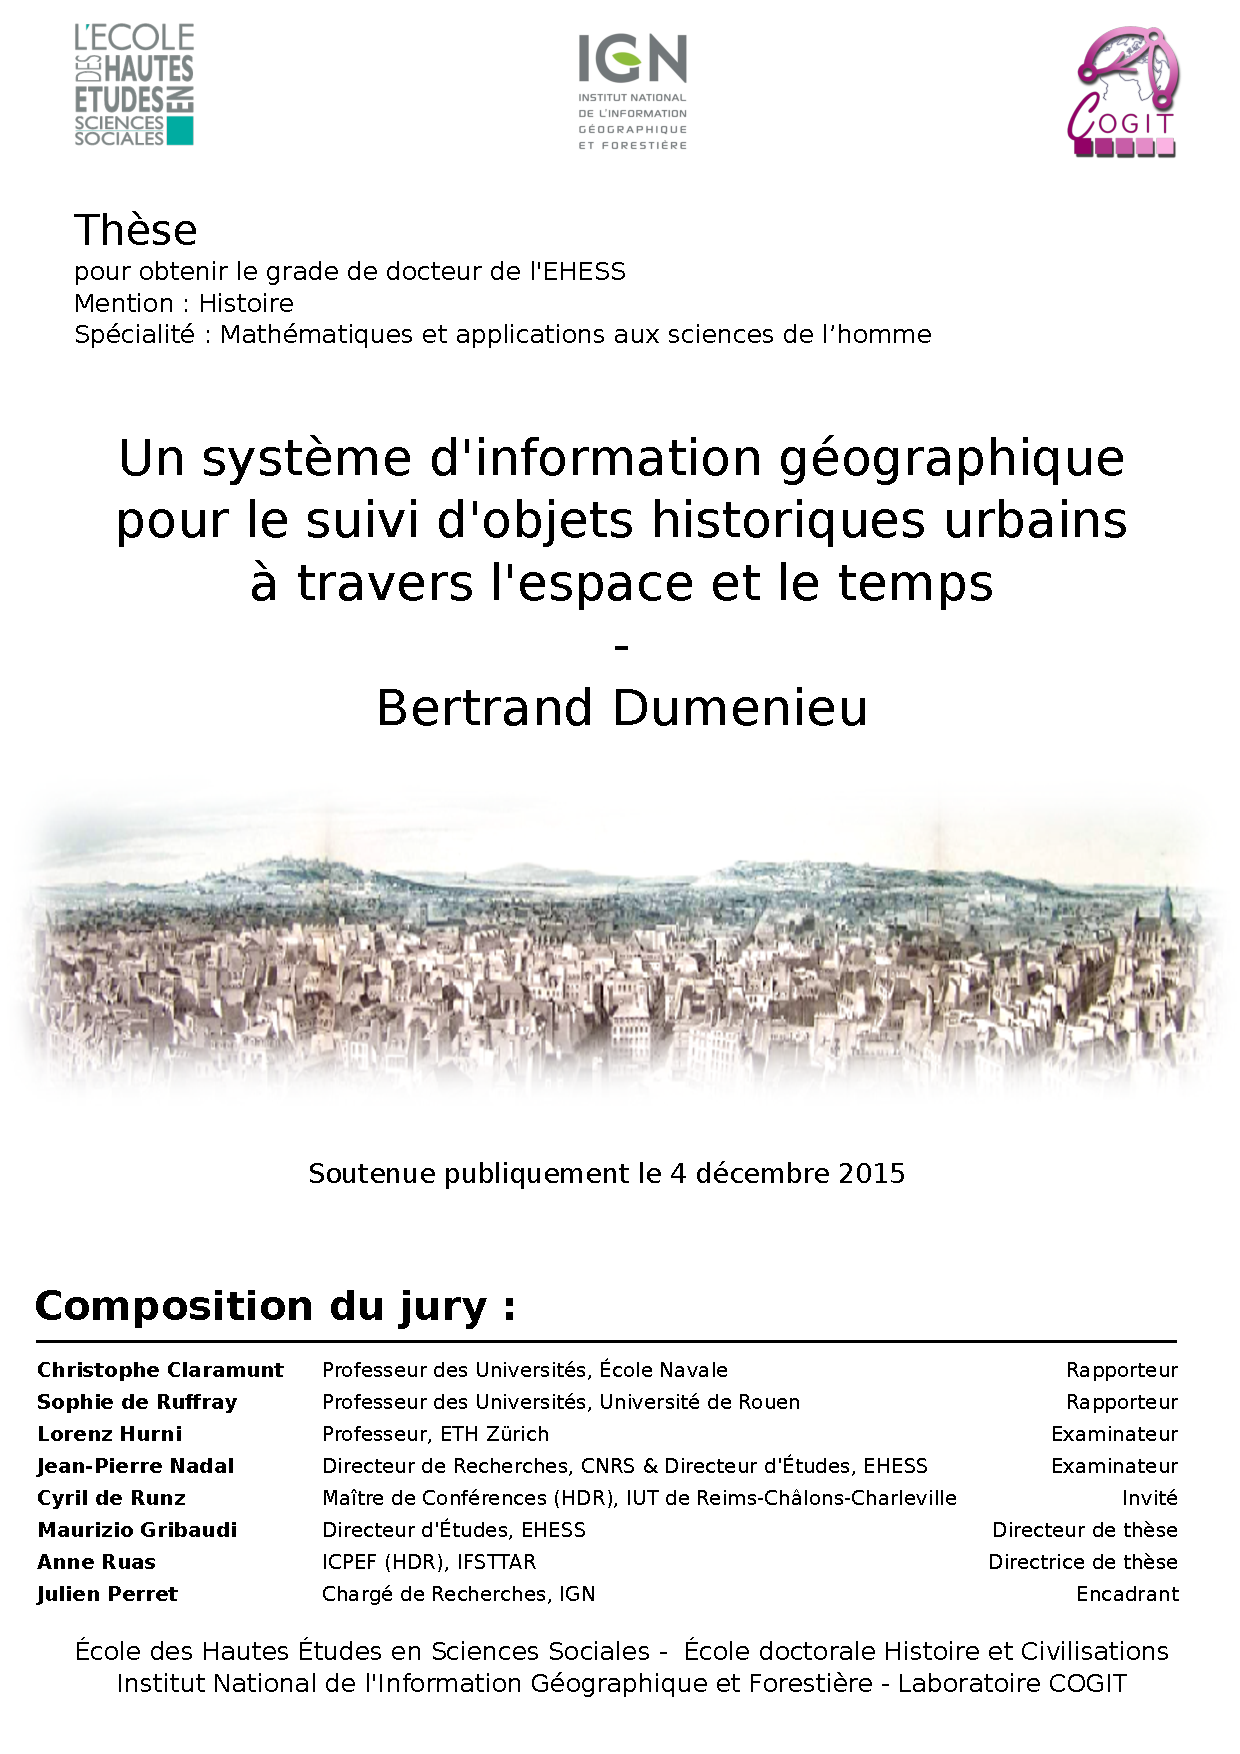
\includepdf[offset=0 -40]{0_couverture/frontcover.pdf}

\blankpage

%\markboth{Table des mati�res}{Table des mati�res}
\dominitoc

\tableofcontents

\newpage\cleardoublepage\thispagestyle{empty}
\addcontentsline{toc}{chapter}{Introduction}
\setcounter{mtc}{1}
\renewcommand\labelitemi{\textbullet}% bullet

\markboth{Introduction}{Introduction}
\chapter*{Introduction}
Depuis le milieu des ann�es 1990, les disciplines historiques montrent un int�r�t grandissant pour les syst�mes d'informations g�ographiques (SIG). En effet, ceux-ci offrent la possibilit� de produire des repr�sentations visuelles des espaces pass�s, soit � partir de repr�sentations cartographiques anciennes, soit en constituant des bases de donn�es spatiales � partir de sources diverses (cartes, donn�es arch�ologiques, connaissances historiques, etc.).Les donn�es produites par des �tudes historiques sur des individus, des �v�nements, ou encore des zones du territoire consid�r�s � un temps donn� peuvent alors �tre associ�es � des r�f�rences spatiales issues de ces bases de donn�es repr�sentant l'espace pass� � une p�riode coh�rente avec le temps valide des donn�es. L'inscription de ces donn�es historiques dans l'espace fournit ainsi de nouvelles perspectives d'analyse et de compr�hension de la r�partition et de l'organisation des ph�nom�nes �tudi�s ainsi que de leurs interactions avec l'espace.Enfin, les SIG constituent de puissants outils de partage des donn�es utiles aux �tudes historiques et de diffusion des connaissances produites par ces �tudes. Les plate-formes cartographiques en ligne et les bases de donn�es spatiales ouvertes offrent de nouveaux outils de diffusion, de visualisation et d'analyse des donn�es historiques spatialis�es. Elles augmentent en outre la r�-utilisabilit� de ces donn�es. Les ph�nom�nes �tudi�s dans le champs de l'histoire sont par essence dynamiques, et leur �tude se situe dans la dur�e. Spatialis�s, ils �voluent dans un espace lui-m�me en constante r�organisation. Ainsi, une repr�sentation statique ne suffit plus et il devient n�cessaire de repr�senter �galement les changements morphologiques qui affectent cet espace au cours du temps. Lorsque les ph�nom�nes dont l'�volution au cours du temps est �tudi�e sont purement spatiaux, comme les transformations d'une ville par exemple, la repr�sentation des dynamiques spatiales au sein d'un syst�me d'information g�ographique offre des outils de visualisation et de mesure de ces changements. Lorsque qu'ils sont sociaux, la confrontation entre dynamiques spatiales et sociales permet de faire appara�tre les interactions qui peuvent exister entre elles~\citep{Knowles2008}.

\paragraph{}
Du point de vue de la g�omatique, cette question de la repr�sentation des �volutions de l'espace se traduit par la production de  bases de donn�es spatio-temporelles. Celles-ci permettent de repr�senter des objets g�ographiques �voluant dans le temps et fournissent un ensemble d'outils permettant d'effectuer des analyses sur ces �volutions.

\paragraph{}
Pour former une base de donn�es g�ographique sur l'espace ancien � une p�riode choisie, deux strat�gies sont possibles. La premi�re consiste � partir d'une base de donn�es de r�f�rence, puis � modifier les objets qui la composent selon les connaissances historiques dont on dispose sur leur �tat et leur existence au moment consid�r�. La seconde strat�gie repose sur des sources cartographiques anciennes qui sont num�ris�es de fa�on � extraire des objets g�ographiques. La premi�re strat�gie n'est envisageable que pour des p�riodes proches de celle de la base de donn�es de r�f�rence pour lesquelles les structures sont connues et peu diff�rentes. Pour cette raison, nous adoptons dans cette th�se uniquement sur la seconde strat�gie. Celle-ci comporte cependant deux inconv�nients majeurs. Tout d'abord, les sources cartographiques anciennes sont h�t�rog�nes~: leur forme, leur objectif et leur contexte diff�rent. En r�sultent des choix d'�chelles, de th�mes cartographiques ou de symbolisation vari�s. M�me lorsqu'elles d�crivent un m�me espace, les pratiques cartographiques contemporaines de leur production aboutissent � des divergences majeures entre cartes comme le recours � des vues obliques ou verticales par exemple. De plus, des diff�rences de pr�cision g�om�trique ainsi que de perfectionnement des techniques de lev� cartographique aboutissent � des cartes distordues pour lesquelles une simple superposition ne suffit pas � saisir les transformations de l'espace trac�. Les objets g�ographiques num�ris�s � partir de sources cartographiques anciennes sont donc, � leur image, h�t�rog�nes.
\paragraph{}
La constitution d'une base de donn�es spatio-temporelle sur l'espace n�cessite de situer les objets g�ographiques dans le temps, cette temporalit� d�pendant de la nature des objets et de l'�tude. Cette datation, effectu�e � partir de connaissances historiques �ventuellement partielles ou incertaines, peut pr�senter des difficult�s. En outre, lorsque les objets sont issus de sources cartographiques, il faut se poser la question de leur statut. S'agit-il d'objets g�ographiques repr�sentant des entit�s du monde r�el et dont la nature influe sur la datation? Ou bien doit-on les consid�rer comme de simples symboles dont l'existence et donc la date sont intrins�quement li�es � celles de la carte qui les renferme? Il faut alors s'interroger sur la temporalit� propre � la source cartographique elle-m�me~: quelle signification donner � l'existence d'une carte?

\paragraph{}
Il existe de nombreux syst�mes d'information g�ographique d�di�s � l'histoire. Pour la plupart, il s'agit d'outils de cartographie en ligne proposant une visualisation de donn�es sociales localis�es sur un fond cartographique ancien. Seuls quelques outils mod�lisent les transformations et s'appuient sur une base de donn�es spatio-temporelle. Ils sont cependant sp�cialis�s pour un cas applicatif pr�cis. L'absence d'outils g�n�riques pour cr�er de telles bases de donn�es s'explique par les diff�rentes difficult�s que nous venons d'�noncer. L'inad�quation entre les fonctionnalit�s des SIG existants et les sp�cificit�s des donn�es historiques constituent un frein � la mise en \oe uvre de tels outils. L'objectif de cette th�se est donc de \textbf{proposer une m�thode de cr�ation de bases de donn�es spatio-temporelles � partir de sources cartographiques anciennes.}

\paragraph{}
�tant donn�e la position interdisciplinaire du sujet qu'il aborde, ce m�moire s'organise en deux parties, chacune adress�e � un des champs disciplinaires concern�s.
\subparagraph{}
La premi�re partie divis�e en deux chapitres, s'inscrit dans le domaine de l'histoire. 
\begin{itemize}
\item[] Dans le \textbf{chapitre 1}, nous posons les bases m�thodologiques d'un mod�le de cr�ation de donn�es spatio-temporelles pour l'�tude historique. Pour ce faire, nous nous int�ressons dans un premier temps aux questionnements des historiens sur l'espace et ses transformations afin de d�gager les deux objectifs g�n�raux d'un outil destin� � mod�liser ces transformations. En analysant un ensemble de travaux historiques, nous identifions trois niveaux d'intrication entre ph�nom�nes sociaux et dynamiques spatiales mettant en �vidence le besoin de donn�es spatio-temporelles pour d�crire ces dynamiques, mais �galement d'outils permettant de les manipuler. Nous proposons ensuite une typologie des sources d'archives permettant de retrouver les transformations de l'espace, avant de nous concentrer plus particuli�rement sur les plans topographiques. Nous montrons par la suite les diff�rentes complexit�s et imperfections spatiales mais aussi temporelles de ces sources. De tous ces �l�ments, nous d�gageons les trois objectifs d'un outil SIG adapt� � l'histoire~:
\begin{itemize}
\item La constitution de donn�es spatio-temporelles pour repr�senter les transformations de l'espace,
\item La mod�lisation et la repr�sentation des imperfections des informations sur l'espace,
\item La conservation d'un lien fort entre les donn�es et les sources historiques d'archives desquelles elles proviennent.
\end{itemize}
Nous confrontons ensuite les diff�rents SIG historiques avec les objectifs identifi�s afin de justifier notre approche m�thodologique ainsi que les objectifs de cette th�se.
\vspace{11pt}
\item[] Dans le \textbf{chapitre 2}, nous proposons une analyse des sources cartographiques parisiennes utilis�es pour extraire des objets g�ographiques sur l'espace de Paris afin d'identifier leurs imperfections propres mais aussi leurs sp�cificit�s et leur contenu. Ce chapitre est �galement l'occasion d'effectuer une critique de ces diff�rentes sources, en particulier dans le cas de l'\emph{atlas national de la ville de Paris} dress� par l'architecte Th�odore Jacoubet. L'�tude de cet atlas nous permet en outre de mettre en lumi�re l'organisation progressive des services de la voirie parisienne au cours du XIX\up{e} si�cle. Enfin, ce chapitre nous permet de mieux conna�tre les temporalit�s de ces diff�rentes sources cartographiques.
\end{itemize}

\subparagraph{}
La seconde partie pr�sente le c\oe ur de notre proposition au fil de 4 chapitres. Ceux-ci r�pondent � la question g�n�rale de la construction d'une base de donn�es spatio-temporelle � partir de repr�sentation de l'espace urbain d�crit par des sources cartographiques anciennes?. Nous d�composons la question en 4 sous-questions, chacune trait�e par un chapitre.
\begin{itemize}
\item[] Dans le \textbf{chapitre 3}, nous abordons la probl�matique du g�or�f�rencement de plans topographiques anciennes de Paris, ainsi que de l'extraction de donn�es g�ographiques vectorielles qui puissent �tre utilis�es pour reconstituer les transformations de la ville. Pour cela, nous proposons une approche de g�or�f�rencement fond�e sur l'utilisation des �l�ments g�od�siques repr�sent�s dans les plans, notamment le carroyage de ceux-ci. Cette approche nous permet, � partir de points de mesure plac�s sur des objets g�ographiques, d'analyser en finesse les distorsions g�om�triques de l'atlas de Verniquet, un grand plan de Paris du XVIII\up{e}.
\vspace{11pt}
\item[] Le \textbf{chapitre 4} pr�sente quand � lui le mod�le de donn�es spatiales et temporelles que nous avons cr��, destin� � stocker les donn�es g�ographiques vecteur issues des cartes. Ce chapitre s'organise autour de deux axes. D'abord, nous proposons un mod�le de base de donn�es fond�e sur les standards de l'information g�ographique visant � repr�senter des objets g�ographiques vectoriels extraits de sources cartographiques tout en conservant une relation de d�pendance forte entre ces objets et leur source. En outre, nous pr�sentons comment ces objets, nomm�s \textbf{observations g�ohistoriques} dans le mod�le, peuvent �tre localis�s dans le temps. Le mod�le finalement propos� organise les observations en couches spatiales et temporelles, ou \emph{snapshots}. La localisation temporelle des observations et de leurs sources �tant souvent difficile � d�terminer avec pr�cision, nous proposons une repr�sentation des temporalit�s par intervalles temporels flous d�crivant la p�riode d'existence des source et des observations g�ohistoriques. Nous d�crivons �galement la m�thodologie adopt�e pour d�finir ces intervalles flous, ce qui nous permet de fixer les temporalit�s associ�es aux sources cartographiques utilis�es. Enfin, � partir d'un �tat de l'art des m�thodes de tri de sous-ensembles flous, nous s�lectionnons deux op�rateurs de base pour raisonner sur des temporalit�s floues, en particulier sur l'ordre temporel et l'ant�c�dence d'un temps sur un autre.
\vspace{11pt}
\item[]Dans le \textbf{chapitre 5}, nous nous int�ressons � la question suivante~: \emph{comment mod�liser et identifier les transformations existantes entre les observations de diff�rentes sources g�ohistoriques?}. Nous y r�pondons en deux temps.
D'abord, nous pr�sentons un mod�le formel de graphe spatio-temporel issu d'un mod�le de la litt�rature, que nous adaptons afin de prendre en compte les sp�cificit�s des donn�es g�ohistoriques. Ce \emph{graphe g�ohistorique} nous permet de repr�senter les transformations existantes entre les observations d'une base de donn�es spatiale et temporelle. Pour identifier ces transformations, nous nous int�ressons ensuite � la notion d'identit� dans le contexte des donn�es spatio-temporelles, et nous proposons un cadre pour d�finir de fa�on souple cette identit� afin de sp�cialiser un graphe g�ohistorique � un cas d'application pr�cis. Nous proposons ensuite un processus de construction d'un tel graphe � partir d'un ensemble d'observations g�ohistoriques structur�es selon notre mod�le de donn�es spatial et temporel. Nous introduisons pour cela une nouvelle structure, appel�e \emph{hypergraphe de processus}, mod�lisant les processus de transformation de l'espace et servant de base � notre m�thode de construction.
\vspace{11pt}
\item[]Enfin, nous proposons dans le \textbf{chapitre 6} une m�thode de construction semi-automatique d'un graphe g�ohistorique � partir d'une d�finition de l'identit� des observations. Pour cela, nous mettons en place une proc�dure en deux temps. D'abord, nous construisons par optimisation stochastique l'hypergraphe de processus d'un ensemble d'observations g�ohistoriques. En identifiant les observations dont les identitit�s sont li�es\footnote{Parce qu'elles repr�sentent une m�me entit� du monde r�el, ou deux entit�s dont l'une est le r�sultat de la transformation de l'autre.}, nous d�couvrons les relations de filiation qui lient les observations entre elles. Ensuite, nous pr�sentons une m�thode fond�s sur la th�orie des fonctions de croyance permettant, � partir d'une certaine d�finition de l'identit�, d'identifier la nature exacte des relations de filiation pr�alablement construites. Ainsi, nous cr�ons un graphe g�ohistorique complet � partir d'observations �parses stock�es au sein de \emph{snapshots} dans la base de donn�es spatiale et temporelle.
\end{itemize}
 %Introduction

%---------------------PARTIE 1---------------------
\part{Positionnement et sources cartographiques sur Paris}


%GLOSSARY ENTRIES
%\newglossaryentry{SIG}{name={SIG}, description = {Syst�me d'Informations G�ographiques.
%Le terme de SIG est polys�mique et se rapporte � plusieurs �l�ments ayant en commun la manipulation, le stockage ou la repr�sentation d'une information g�ographique.
%Il peut s'agir d'un ensemble organis� de mat�riels informatiques, de logiciels, de donn�es g�ographiques et de personnel capable de saisir, stocker, mettre � jour, manipuler, analyser et pr�senter toutes formes d'informations g�ographiquement r�f�renc�es~\citep{Blomac1994}.
%Le terme est par ailleurs utilis� pour d�signer un ensemble de donn�es rep�r�es dans l'espace, structur� de fa�on � pouvoir en extraire commod�ment des synth�ses utiles � la d�cision~\citep{Didier1990}}}

\chapter{Positionnement du sujet}
\renewcommand{\labelitemi}{\tiny$\blacksquare$}

\large \begin{mybox} \normalsize
\textbf{Objectifs~:} 
\vspace{11pt}
\begin{itemize}
\item  Explorer l'ad�quation entre l'utilisation de l'espace par les historiens et les fonctionnalit�s offertes par les SIG historiques existants.
\vspace{11pt}
\item  Identifier les complexit�s des donn�es g�ohistoriques.
\vspace{11pt}
\item  Formaliser la probl�matique de la th�se et se positionner par rapport � elle.
\end{itemize}
\end{mybox}
\renewcommand\labelitemi{\textbullet}% bullet
\newpage
\minitoc
\newpage

\label{chap:positionnement}
\paragraph{}
\begin{quotation}
%\emph{J'aimerais qu'il existe des lieux stables, immobiles, intangibles, intouch�s et presque intouchables, immuables, enracin�s~; des lieux qui seraient des r�f�rences, des points de d�part, des sources : mon pays natal, le berceau de ma famille, la maison o� je serais n�, l'arbre que j'aurais vu grandir (que mon p�re aurait plant� le jour de ma naissance), le grenier de mon enfance empli de souvenirs intacts. De tels lieux n'existent pas, et c'est parce qu'ils n'existent pas que l'espace devient question, cesse d'�tre �vidence, cesse d'�tre incorpor�, cesse d'�tre appropri�. L'espace est un doute~: il me faut sans cesse le marquer, le d�signer~; il n'est jamais � moi, il ne m'est jamais donn�, il faut que j'en fasse la conqu�te.} Esp�ces d'Espaces, George Perec, 1974.
\emph{Le pass� ne se conserve pas, mais fait l'objet d'une reconstruction toujours recommenc�e.}\\
 Carnets de croquis. Sur la connaissance historique , Bernard Lepetit, 1999.
\end{quotation}
\paragraph{}
Ce chapitre propose d'explorer plus avant les raisons de l'inad�quation entre des outils informatiques, pourtant destin�s � g�rer des donn�es spatiales, et la pratique historique d'un espace urbain.Apr�s avoir formalis� et d�fini les particularit�s de l'information g�ographique utilis�e en histoire -d�sign�e alors par le terme \textit{g�ohistorique}- et expos� les diff�rentes sources d'information g�ographiques utilis�es dans le cadre de recherches historiques sur l'espace urbain,
nous nous attacherons � d�crire le processus d'int�gration d'une information au sein d'un SIG historique afin d'identifier les diff�rentes sources d'imperfections dans les sources et l'information utilis�e. Enfin, nous pr�senterons diff�rents travaux existants visant � manipuler une information g�ohistorique imparfaite dans le cadre des syst�mes d'information g�ographiques.
\subparagraph{}
D'abord, nous regarderons du cot� des utilisations de l'espace urbain en histoire afin d'identifier les besoins et attentes sp�cifiques des historiens.
Pour ce faire, nous commencerons dans la section~\ref{section:usages} � mettre en lumi�re les pratiques des historiens et leurs probl�matiques gr�ce � l'analyse d'un espace urbain.
Dans la section~\ref{subsection:sources}, nous pr�senterons une typologie des diff�rentes ressources permettant de reconstruire une repr�sentation d'un espace urbain ancien.
Il s'agira non seulement d'explorer les diff�rentes sp�cificit�s de ces ressources, mais �galement d'en identifier les complexit�s.
Ainsi, nous pourrons expliciter clairement les objectifs des historiens quant aux usages de l'espace urbain au sein de leurs �tudes, et par l� identifier les demandes adress�es par l'�tude historique � des outils permettant de manipuler et repr�senter des donn�es g�ographiques.
\subparagraph{}
Dans un second temps, nous nous int�resserons plus pr�cis�ment aux syst�mes d'informations g�ographiques et � leurs usages pour des �tudes historiques.
Nous aborderons dans la section~\ref{section:SIG} le regard des historiens sur les SIG historiques � partir de la litt�rature de fa�on � classifier les diff�rents objectifs et probl�mes pos�s � l'encontre des SIG par les chercheurs en histoire.
Cette section permettra �galement de terminer la description du processus de reconstruction de l'espace et d'�tablir, dans la section~\ref{section:imperfections}, une typologie des diff�rentes imperfections de la repr�sentation obtenue li�es aux sources, aux donn�es et au traitement d'une information historique et spatiale - g�ohistorique- au sein d'un SIG.
\subparagraph{}
Finalement, nous croiserons ces deux regards pour analyser les syst�mes d'informations g�ographiques destin�s � l'histoire existants dans la litt�rature.
Ainsi, dans la section~\ref{subsection:currgis}, les propositions existantes seront confront�es aux attentes et aux complexit�s identifi�es dans les sections pr�c�dentes.
De cette fa�on, nous montrerons les points d'ad�quation, mais �galement les manques des propositions existantes.
En particulier, nous nous positionnerons (section~\ref{section:positionnement}) par rapport aux probl�matiques d'int�gration de l'information historique issue des repr�sentations anciennes de l'espace urbain, et de mod�lisation des dynamiques des structures composant cet espace.

\section{Analyser l'espace pour comprendre l'�volution d'une soci�t� urbaine}
\label{section:usages}
\subsection{Le choix de l'espace}
\myparagraph{�l�ments de d�finition}
Dans le travail pr�sent� ici, l'espace occupe une place pr�pond�rante.
Celui de la ville, dans son organisation et ses transformations au cours du temps constitue le vecteur d'int�gration de l'information historique.
�tant donn� ce statut central, il nous para�t essentiel de fixer les fronti�res de ce terme dans le cadre d'un travail se situant quelque part entre g�omatique et histoire.
En effet, l'espace englobe des r�alit�s vari�es, li�es aux sensibilit�s des disciplines qui manipulent ce concept, allant de l'espace physique, isotrope et homog�ne � un espace totalement li� aux hommes, produit des soci�t�s qui le construisent \citep{Lefebvre2000}.
L'espace est en premier lieu une notion g�ographique que Pumain et Saint-Julien \citep{Pumain1993,Pumain1997} d�clinent sur deux axes~:
\begin{itemize}
 \item Soit il s'agit de l'espace physique, \emph{ensemble de lieux (ou objets localis�s) muni d'une distance entre ces lieux}.
Il est le \emph{simple contenant des objets} qui permet d'analyser leurs relations.
 \item Soit il s'agit d'un \emph{ensemble de lieux et de relations entre eux, d�finies par les interactions entre des acteurs sociaux localis�s. C'est le produit de l'organisation et de la nature, agent du maintien et du d�veloppement des soci�t�s sur leur territoire}.
\end{itemize}
On parle alors g�n�ralement d'espace \textbf{support} et d'espace \textbf{produit}, le premier �tant vu comme le \textbf{socle immuable sur lequel se situent les faits sociaux}, le second �tant pleinement \textbf{model� par les activit�s des soci�t�s qui l'occupent}\citep{DiMeo1991}.
Des nombreux travaux, tels ceux, fondateurs, de \cite{Roncayolo2011} et \cite{Lepetit1980}, abordent les relations entre histoire et g�ographie et dressent, pour les sciences sociales, le portrait d'un espace intrins�quement li� aux soci�t�s, produit d'une construction constante et renouvel�e \footnote{Le mouvement au sein des sciences humaines qui donne � l'espace une r�le majeur en l'utilisant comme outil de compr�hension des ph�nom�nes sociaux est d�sign� par l'expression \emph{spatial turn}.
Les sp�cificit�s de cette tendance ont �t� abord�e notamment par \cite{Cosgrove1984}, ou plus r�cemment \cite{Torre2008}.}.
Partant de cet angle de vue, notre espace est donc bien physique, topographique, mais impliqu� dans une relation avec les ph�nom�nes sociaux qui l'inscrivent fortement dans la dimension temporelle.
Dans tous le reste du document, le mot ''espace'' fera r�f�rence � cet espace produit.
Quant � l'espace urbain, nous choisissons de le d�limiter par la fronti�re administrative de la ville, �largie �ventuellement � ses abords imm�diats.
Dans le Paris ancien, il s'agit de l'�tendue � l'int�rieur de l'enceinte des Fermiers G�n�raux, � laquelle s'ajoute les communes annex�es en 1860\footnote{On d�vie ici l�g�rement de la d�finition habituelle o� l'espace urbain repose sur la continuit� du b�ti \citep{Moriconi1993}.
Dans le Paris ancien, cette continuit� n'existe que dans un espace central restreint, o� elle est rapidement bris�e par les espaces vides ou cultiv�s � l'int�rieur m�me des enceintes.}.
Cette articulation profonde entre espace g�ographique et temporalit� se trouve notamment � la racine des travaux de Braudel \citep{Bataillon1950, Braudel1951}, qui plaide pour une �tude des ph�nom�nes sociaux inscrite dans un espace g�ographique en transformation (ce qu'il nommera la \emph{g�ohistoire}).
Il consid�re trois couches imbriqu�es de temporalit�s qui constituent l'histoire~: la premi�re est celle des individus, rapide et nerveuse, c'est \emph{une agitation de surface}.
La seconde temporalit� est plus lentement rythm�e, c'est celle des groupements, des civilisations, de l'�conomie et des soci�t�s.
La derni�re, pratiquement fig�e, correspond aux rapports des Hommes avec le milieu qui les entourent, avec l'espace support de leur �tablissement.
L'espace de l'histoire, produit des soci�t�s, est donc inscrit dans des temporalit�s aux rythmes multiples.
S'il nous faut pr�ciser les formes de l'espace urbain qui nous occupent ici, il nous faut dans le m�me temps d�finir les temporalit�s particuli�res que nous consid�rons.

\myparagraph{Int�grer le temps pour �tudier la ville}
Pour Lepetit, reprenant Braudel \citep{Lepetit1986}, l'espace g�ographique est une dimension suppl�mentaire pour l'histoire , constitu� de \emph{valeurs dormantes} (par exemple les axes de circulations marchands) s'offrant � l'analyse historique.
La ville, au travers de ses structures, de son organisation, est alors un \emph{conservatoire temporel} \citep{Lepetit1986} offrant � l'historien des fragments de ses configurations pass�es.
Cette id�e d'une ville constitu�e d'une accumulation de temporalit�s pass�es, dans la lign�e de Roger Dion \citep{Courville1995} \footnote{\emph{Tout paysage humanis� est le reflet d'une histoire, [...] un amalgame d'apports in�gaux en �ge.} Roger Dion, d'apr�s \cite[p. 20]{Courville1995}} sera de nouveau exploit�e par \cite{Lepetit1996}, pour qui l'histoire int�gre par la dimension temporelle les consid�rations sociales, politiques, �conomiques sur la ville.
L'�tude de la ville en histoire -l'histoire urbaine- est alors un moyen de compr�hension de l'�volution d'une soci�t� au travers de son �tude sur le temps long \footnote{L'arch�ologie fait un large usage de ce terme pour d�signer des p�riodes de plusieurs si�cles ou mill�naires \citep{Redman2003}.
En histoire, les p�riodes d'�tude sont souvent plus restreintes.
Nous d�signons par le terme ''temps long'' toute dur�e suffisamment grande pour que des changements sensibles dans l'organisation de l'espace se produisent.
Dans l'espace parisien du XIX\up{e} si�cle, quelques dizaines d'ann�es suffisent pour modifier en profondeur les r�seaux de rues et l'organisation du b�ti}.
\cite{Perrot1975} invoque �galement cette inscription de la ville dans le temps -pour l'Europe tout du moins-, arguant que la compr�hension de l'urbanisation et de ses formes repose sur des processus de transformations urbaines dans la longue dur�e.
L'histoire urbaine inscrit donc l'espace de la ville dans le temps pour en �tudier les transformations et les mettre en rapport avec les ph�nom�nes sociaux qui s'y sont d�roul�s.
\subparagraph{}
Pour Roncayolo (d'apr�s \cite{Walter2005}), \emph{les pierres et les formes urbaines sont du temps et des pratiques consolid�es}.
Attach� � faire appara�tre les divisions sociales au travers de ses \emph{lectures de villes}, il y d�crypte les relations entretenues par les portions d'espace et les formations sociales.
Ces relations se lisent alors dans la construction de l'espace urbain, c'est-�-dire son inscription dans diff�rentes \emph{couches temporelles} aux rythmes vari�s~-le temps devient alors le \emph{tempo}-, aboutissant � des d�calages, des ruptures qui se lisent dans cette construction urbaine.
Son �tude des limites de Marseille et Paris aux XIX et XXe si�cles, d'abord mat�rialis�es par des enceintes puis persistant au travers de limites symboliques, s'appuie � la fois sur l'organisation et les transformations des structures urbaines mais aussi sur des consid�rations sociales (contraintes militaires, op�rations immobili�res et financi�res, etc.) et symboliques (repr�sentation mentales de la ville et de ses limites) \citep{Walter2005}.
\subparagraph{}
D'apr�s ces historiens, il s'agit donc d'�tudier les structures de la ville, son organisation, des r�seaux de voies de communication aux transformations des structures b�ties qui la composent.
Pourtant, comme le fait remarquer \cite{Lemas2009}, le champ de l'histoire urbaine n'est pas homog�ne et l'importance prise par l'espace urbain dans l'�tude varie largement.
Cette h�t�rog�n�it� se traduit notamment par des degr�s d'importance attribu�s aux dynamiques de l'espace dans l'�tude historique, conditionnant alors la place prise par la dimension spatiale dans l'�tude.
Nous faisons ici l'hypoth�se que ces diff�rents usages vont conditionner les attentes des historiens, et donc les outils et les m�thodes appropri�s.
Il est alors n�cessaire d'identifier les diff�rents usages de l'espace de la ville en histoire de fa�on � nous positionner efficacement par rapport aux diff�rents besoins des historiens, et � pouvoir analyser l'ad�quation des outils existants avec ces besoins.

\subsection{Quels usages de l'espace urbain en histoire?}
Dans le paragraphe pr�c�dent, nous avons expliqu� que l'espace g�ographique en histoire �tait toujours trait� comme un produit r�sultant des activit�s humaines.
Pourtant, nous allons le voir, la place occup�e par l'espace de la ville est tr�s variable au sein de l'historiographie.
Nous proposons alors d'explorer cette vari�t� au travers de trois modalit�s fond�es sur l'importance de la relation entre l'espace �tudi� et le temps.
Nous choisissons volontairement de ne pas consid�rer les ph�nom�nes sociaux �tudi�s comme variable de contr�le car leur vari�t� et leur h�t�rog�n�it� emp�cheraient tout regroupement.
Les dynamiques spatiales se m�lent d'autant plus aux dynamiques sociales �tudi�es que la liaison entre espace et temps augmente.
Ce couplage a cependant un co�t~: il implique un faible degr� d'abstraction de l'espace et une finesse temporelle importante.
Il conditionne donc les besoins des historiens en termes de mod�les et de repr�sentations de l'espace.
Dans les paragraphes suivants, nous pr�sentons ces diff�rents niveaux d'int�gration du temps et identifions les besoins qui leur sont sp�cifiques � partir de diff�rents travaux en histoire.
Bien s�r, les exemples abord�s ne constituent qu'une infime partie de la production en histoire urbaine, cependant nous consid�rons qu'ils illustrent correctement le propos.
% 
% La pratique de l'espace peut �tre particularis�s pour chaque �tude historique, d�pendant de la p�riode, de la zone g�ographique et du sujet d'�tude.
% Nous choisissons ici de d�limiter des cat�gories g�n�rales de prise en compte de la dimension spatiale en histoire en suivant les travaux de \cite{Arnaud2008} sur l'espace de la ville.
% D'abord, l'espace  peut �tre utilis� comme simple cadre de l'�tude, se pla�ant alors comme contexte d'un probl�me d'avantage que comme un v�ritable support de travail.
% Lorsqu'il prend de l'importance dans l'�tude, l'espace devient alors un outil servant � mettre en rapport les donn�es historiques sociales, �conomiques ou bien encore d�mographiques.
% Finalement, l'espace devient objet d'�tude et il s'agit alors de s'int�resser � son organisation, aux transformations qui l'affectent dans le temps de fa�on � lire � travers ses formes les ph�nom�nes sociaux qui le mod�lent \citep{Lefebvre2000}.
% Comprendre ces trois niveaux dans l'appr�hension de l'espace en histoire illustre les motivations des historiens dans leur usage de l'espace et par l� d�finit les objectifs vis�s par l'utilisation d'un SIG en histoire.

\myparagraph{L'espace urbain~: cadre de l'�tude}
Mettre en relation un ph�nom�ne social avec un espace g�ographique constitue le premier niveau de prise en compte de l'espace en histoire.
Cette mise en relation implique de situer dans l'espace les diff�rents ph�nom�nes et faits �tudi�s, construisant ainsi le contexte g�ographique de l'�tude historique.
� la mani�re d'un fond cartographique servant de base � la repr�sentation graphique d'une information g�ographique, l'espace sous-tend et illustre le propos historique, mais son organisation n'en constitue un �l�ment d'explication qu'� un niveau d'abstraction et une �chelle �lev�s.
\subparagraph{}
Dans son travail sur le cosmopolitisme dans les villes m�diterran�ennes et plus particuli�rement celles de l'empire Ottoman, \cite{Lafi2011} explore les diff�rentes formes de ce ph�nom�ne, les rapports de pouvoirs entre communaut�s au travers du prisme des volont�s politiques des diff�rents r�gimes (empire Ottoman et royaumes occidentaux notamment), des valeurs port�es par les religions et des traits culturels locaux.
Ainsi, si la ville se trouve au c\oe ur de cette �tude, son espace n'est que tr�s peu consid�r�.
En effet, l'�vocation des villes par leurs noms fournit surtout une toile de fond sur laquelle est dessin�e l'�tude, servant � diff�rencier les formes de cosmopolitisme par la ville et sa position dans de grandes zones g�ographiques (par exemple le nord de la M�diterran�e).
Si le ph�nom�ne s'inscrit dans le temps tout au long de l'�tude, l'espace quant � lui est fig�.
Il reste tr�s abstrait, �voqu� uniquement par des noms de lieux, d'aires culturelles et constitue, � proprement parler, le support de l'�tude.
L'organisation interne des villes n'est alors pas objet d'�tude, bien qu'elle se lise par exemple en filigrane dans l'�vocation de l'identit� communautaire des quartiers (par exemple � Tripoli).
Cet espace n'est pourtant pas totalement neutre.
En effet, la situation portuaire de certaines villes est d�velopp�e pour expliquer certains profils de cosmopolitisme.

\begin{wrapfigure}{r}{80mm}
	\centering
		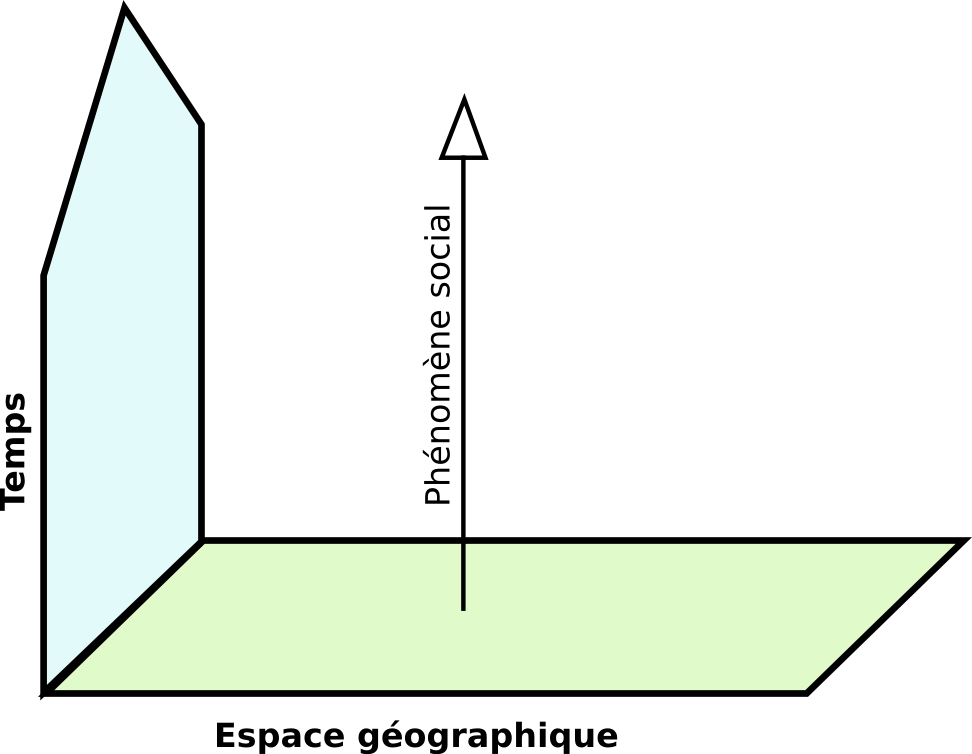
\includegraphics[width=0.4\textwidth]{spaceuse1.png}
	\caption{Premier niveau d'int�gration de l'espace urbain~: c'est un cadre servant de contexte, implicitement situ� dans le temps par le th�me de l'�tude.
La dimension temporelle  est dominante.
\textcolor{cyan}{\textbf{T}}}
	\label{fig:spaceuse1}
\end{wrapfigure}
\subparagraph{}
Dans son travail sur la notion \emph{d'habiter} dans les villes italiennes, \cite{Barbot2013} s'inscrit plus directement dans l'espace urbain, �tudiant pour plusieurs villes d'Italie les pratiques sociales li�es au fait d'habiter la ville et les rapports de forces entre les couches de la soci�t�.
Plus particuli�rement, l'auteur montre parfaitement la cons�quence de ces pratiques sur l'espace, les diff�rentes couches sociales pr�sentes dans la ville �tant visibles au travers des types d'habitats correspondant � leur degr� d'int�gration dans la ville.
Cet espace constitue un cadre dans lequel viennent se placer les diff�rentes formes de l'appartenance � la ville, mais son organisation interne ou sa situation g�ographique ne sont pas des facteurs de compr�hension de ces appartenances.
La ville reste un objet abstrait, spectateur d'une �tude dont le sujet porte essentiellement sur les rapports sociaux.

\subparagraph{}
Au travers de ces deux travaux, nous pouvons voir appara�tre un premier niveau o� l'intrication du temps et de l'espace urbain est tr�s peu pr�sente.
Si le ph�nom�ne social s'inscrit toujours dans le temps, l'espace urbain est quant � lui fig� dans une temporalit� longue.
Il constitue le contexte du propos plut�t qu'un objet d'�tude � part enti�re (voir figure \ref{fig:spaceuse1}).
L'�tude n'est pas spatiale, mais fait r�f�rence � l'espace, elle reste purement temporelle.
En marge de l'�tude, il peut �tre abord� de fa�on tr�s abstraite \citep{Arnaud2008}, ses formes apparaissant en filigrane par l'�vocation des quartiers, des s�parations entre groupes sociaux ou des positions relatives des objets abord�s.
Dans les deux cas, l'�chelle est relativement grande, permettant d'englober tout l'espace concern� par le ph�nom�ne �tudi�.

\myparagraph{L'espace urbain outil d'�tude} 
\label{paragraph:space_as_tool}
D'autres auteurs trouvent dans l'organisation de l'espace un outil de compr�hension des ph�nom�nes qu'ils �tudient.
Il s'agit alors la plupart du temps d'aborder l'espace comme un support sur lequel l'on vient localiser des donn�es sociales dans le but de faire appara�tre des configurations particuli�res et des relations jusqu'ici invisibles.
Il s'agit finalement de consid�rer que \emph{la distribution des ph�nom�nes dans l'espace n'est pas neutre dans la mani�re dont ils �voluent et se transforment} \citep{Arnaud2008}.
Il ne s'agit donc pas encore d'�tudier l'organisation et les formes de l'espace en elles-m�mes, mais de lire au travers d'elles des propri�t�s, des relations entre les ph�nom�nes �tudi�s que seule leur situation dans l'espace de la ville permet de faire appara�tre efficacement (citons par exemple les travaux de \cite{Marraud2010} sur les corporations parisiennes aux XVII\up{e} et XVIII\up{e} si�cles, appuyant dans l'espace de Paris son analyse des r�sistances et des transformations de la corporation des boulangers au gr� des rapports de forces qu'elle entretient avec le pouvoir royal et de l'ordre public).
\begin{wrapfigure}{r}{80mm}
  \centering
  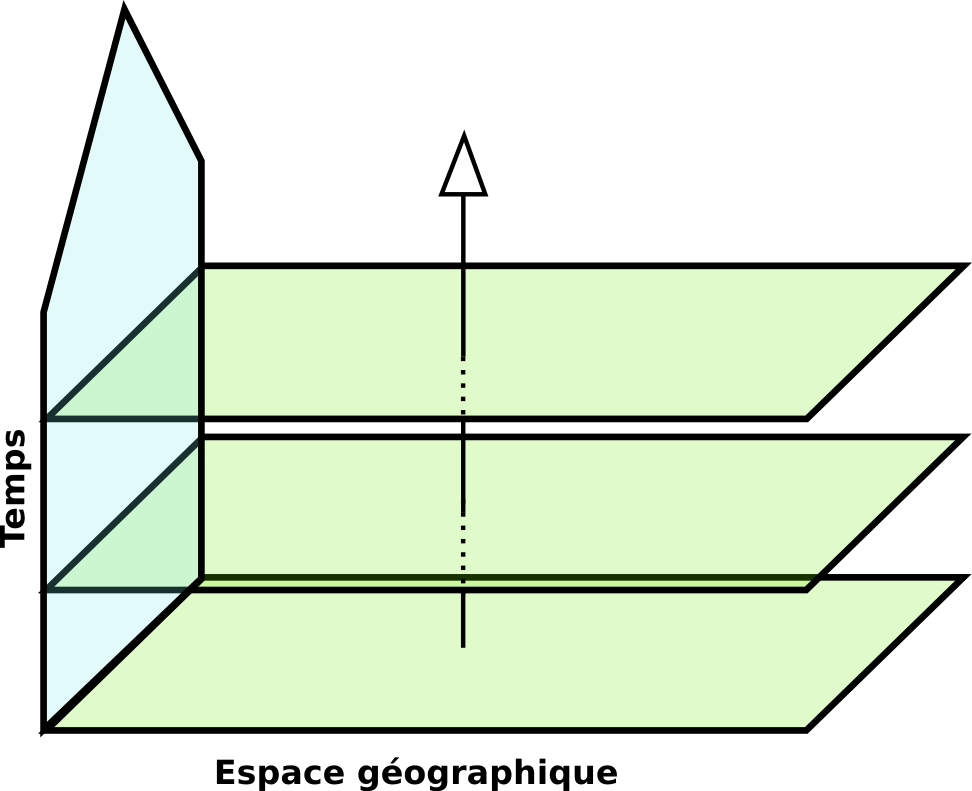
\includegraphics[width=0.4\textwidth]{spaceuse2.png}
  \caption{Second niveau d'int�gration de l'espace urbain~: l'espace devient un outil d'analyse des donn�es sociales permettant de les r�partir dans la ville.
Les dimensions spatiales et temporelles sont consid�r�es conjointement (\textcolor{green}{\textbf{S}}+\textcolor{cyan}{T})}
  \label{fig:spaceuse2}
\end{wrapfigure}
\subparagraph{}
L'espace g�ographique est aussi un outil de compr�hension des ph�nom�nes sociaux.
Inscrits dans celui-ci, leur r�partition et organisation offre de nouvelles pistes de r�flexion et d'analyse.
Il s'agit en quelque sorte de mettre les ph�nom�nes � l'�preuve de l'espace.
On peut en particulier citer les travaux de \cite{Gauthiez2010} qui restituent � partir de textes d'archives les trajets des milices bourgeoises au XVII\up{e} si�cle dans un parcellaire de la ville de Lyon, permettant alors de mettre en �vidence diff�rents profils de parcours et faisant na�tre de nouvelles questions li�es aux formes de ces parcours et � leurs transformations.
\cite{Weiss2009} dans ses travaux sur les censives parisiennes inscrit directement les rapports sociaux entre propri�taires parisiens.
Les divers conflits juridiques se transcrivent dans l'espace de la ville par des zones o� l'appartenance � une censive \footnote{La censive est une terre appartenant � un seigneur, dont il c�de certains droits en �change d'une redevance~: le cens.}
est mal d�finie.

\subparagraph{}
Ces �tudes\footnote{On peut encore citer \cite{GonzalezQuijano2012} ou bien \cite{Montel2013}} s'appuient g�n�ralement sur des m�thodes d'analyse spatiale, en particulier sur des repr�sentations cartographiques des ph�nom�nes dans lesquelles des donn�es qualitatives (par exemples les surfaces des censives) ou quantitatives discr�tis�es (statistiques notamment) sont rendues visibles.
La carte est un puissant outil d'interrogation d'un espace pass�, fournissant une vue globale de l'organisation spatiale des donn�es, mais �galement un outil permettant de remettre en question les faits historiques analys�s \citep{Arnaud2008}.
\subparagraph{}
Cette fois l'espace urbain est consid�r�, � la mani�re de \cite{Lepetit1996}, comme un t�moin des activit�s humaines, une construction qui se donne � lire et permet d'extraire une connaissance sur un fait historique.
L'espace n'est plus abstrait, il est reconstruit � partir des traces qui en subsistent - plans, textes, etc.-, l'�tude �tant tributaire des sources de descriptions existantes.
Cet espace reconstruit est alors situ� dans le temps, mais il s'agit encore d'un socle d'�tude, ses transformations ne font pas l'objet d'une attention particuli�re.
Lorsque le ph�nom�ne social �volue dans le temps, l'espace doit �tre reconstruit de nouveau � partir d'autres sources pour que sa forme et son contenu soient contemporains du ph�nom�ne.
La ville est alors trait�e comme une accumulation de tranches temporelles, comme illustr� dans la figure \ref{fig:spaceuse2}.
L'�tude se place cette fois dans un cadre � la fois spatial et temporel.

\myparagraph{L'espace urbain~: objet d'�tude}
Si l'on consid�re que l'espace urbain est un produit des activit�s humaines, son organisation et ses structures gardent la m�moire des activit�s humaines pass�es (C'est ce qu'Arnaud \cite[p. 141]{Arnaud2008} nomme \emph{hypoth�se de permanence}).
Il devient donc un outil de lecture au travers duquel il est possible de recomposer une histoire urbaine.
Ces traces se trouvent accumul�es dans l'espace, transcrites notamment par les brisures ou au contraire les persistances des structures urbaines \citep{Ducom2009}.
L'enchev�trement qui en r�sulte doit �tre d�crypt�, en \emph{d�roulant} l'histoire de la ville, � partir des structures persistantes, des connaissances des structures pass�es et des �v�nements ayant affect� telle ou telle structure.
On peut citer en exemple les travaux de \cite{Boudon1977}, analysant dans le d�tail les transformations du quartier des Halles � Paris dans le temps long.
\subparagraph{}
L'objectif n'est pas seulement de retracer les transformations de la ville, mais de consid�rer qu'il existe une boucle de r�troaction entre l'espace g�ographique et les ph�nom�nes sociaux, lisible uniquement dans le temps.
Ainsi, lorsqu'il �tudie les �volutions de l'espace social dans un �lot parisien aux XVIII\up{e} et XIX\up{e} si�cles (voir figure \ref{fig:ilot_trinite}), \citep{Gribaudi2009} place l'organisation spatiale de l'�lot au c\oe ur de l'�tude.
Ancien h�pital nationalis� sous la R�volution, l'�lot se transforme petit � petit en un espace dense et vivant compos� d'ateliers d'artisans et de commer�ants.
Ces transformations, loin d'�tre homog�nes dans leurs localisations et leurs rythmes sont abord�es comme le produit de pratiques locales (la sp�culation immobili�re) et globales (la vente des biens nationaux \footnote{Les biens nationaux correspondent aux biens de l'�glise et les domaines seigneuriaux nationalis�s � la suite du d�cret du 2 novembre 1789.}).
Inversement, les pratiques sociales sont mises en rapport avec la perception de l'espace �lot au travers des perceptions des habitants, mais aussi des administrateurs et observateurs ext�rieurs.
D'autres auteurs effectuent le m�me travail de mise en relation, par exemple pour �tudier les �volutions du prix du foncier selon les restructurations du parcellaire parisien \citep{Bove2012}, ou bien encore pour retracer l'�volution des structures urbaines (parcellaire et voirie) d'un espace local � Tours \citep{Lefebvre2009}.
\subparagraph{}
Cette fois l'organisation de l'espace urbain lui m�me est analys�e, soit ind�pendamment de donn�es sociales particuli�res (l'espace est alors consid�r� comme gardant la m�moire des activit�s qui l'ont model� \citep{Roncayolo2011}), soit en relation avec un ou plusieurs ph�nom�nes sociaux.
Lorsqu'il s'agit de l'organisation de l'espace seul, l'analyse morphologique via la repr�sentation cartographique des espaces anciens en constitue le principal outil d'exploration \citep{Arnaud2008}.
Ins�r�e dans le temps, l'analyse morphologique doit �galement s'int�resser aux changements qui affectent les formes urbaines.
Elle peut �tre visuelle, par la mise en correspondance de cartes du m�me espace � des instants diff�rents (c'est le cas par exemple de l'espace �tudi� par \cite{Lefebvre2009}), ou bien s'appuyer sur des indicateurs morphologiques (\cite{Strano2012} ou \cite{Barthelemy2013} par exemple) qui �tudient les transformations des r�seaux de rues dans la r�gion de Milan, puis � Paris via les d'indicateurs structurels sur ces r�seaux).
Finalement, lorsque l'�tude porte sur les relations entre le d�roulement des ph�nom�nes sociaux et les transformations de l'espace urbain, l'analyse morphologique vient compl�ter l'analyse spatiale.
\begin{figure}[ht]
	\centering
		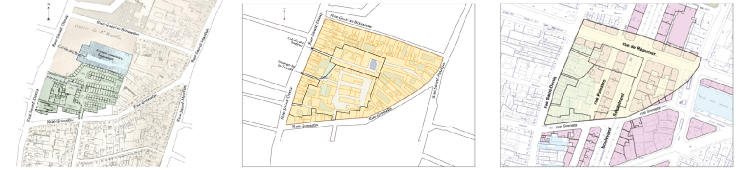
\includegraphics[width=1\textwidth]{trinite.png}
	\caption{Transformations des structures morphologiques de l'�lot de la Trinit� � Paris sur trois p�riodes : au milieu du XVIII\up{e}, en 1845 et apr�s les perc�es haussmanniennes.
Illustration extraite de \cite{Gribaudi2009}.}
	\label{fig:ilot_trinite}
\end{figure}
\subparagraph{}
Recomposer un espace dans toute la complexit� de ses transformations implique un important volume d'informations d�crivant les structures urbaines, leur organisation et les �v�nements qui les affectent.
Par cons�quent, les espaces trait�s sont souvent restreints mais font l'objet d'une description extr�mement pr�cise.
L'espace est alors intiment li� au temps, en interaction continue avec les ph�nom�nes sociaux qui y prennent place.
L'�tude n'est plus seulement spatiale et/ou temporelle car les deux dimensions sont indissociables~: elle devient \textbf{spatio-temporelle}.

\begin{figure}[ht]
  \centering
  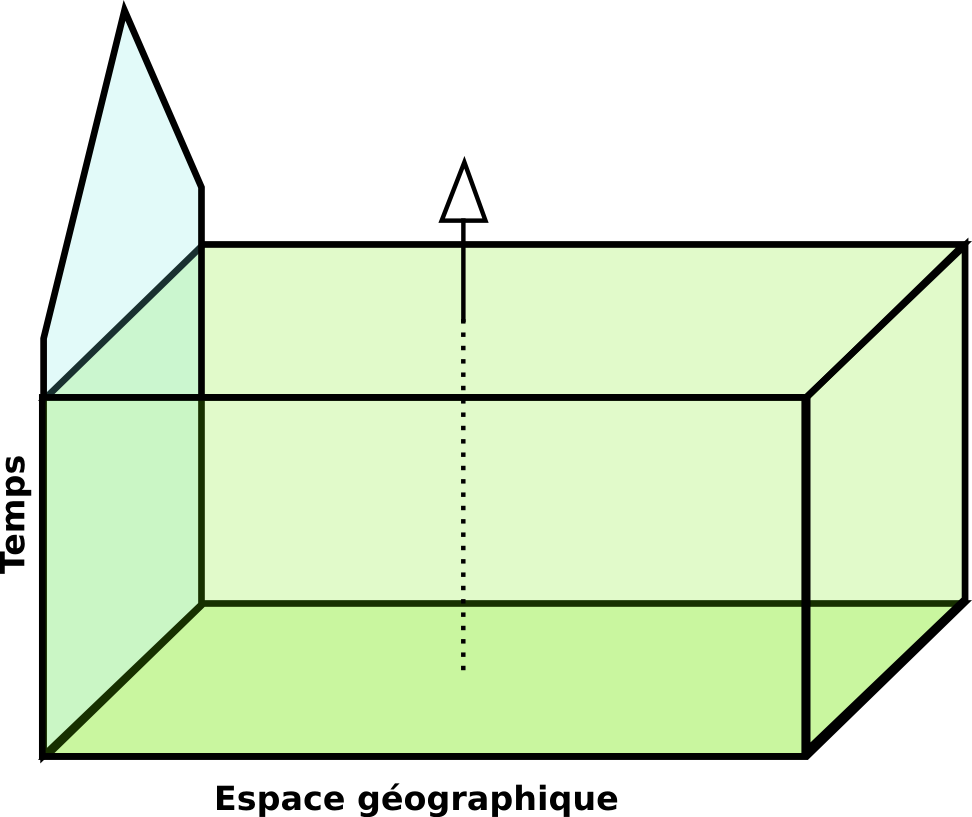
\includegraphics[width=0.4\textwidth]{spaceuse3.png}
\caption{Troisi�me niveau d'int�gration de l'espace urbain~: l'espace en transformation constante est mis en rapport avec les ph�nom�nes sociaux �tudi�s, chacun am�liorant la compr�hension de l'autre.
L'espace devient dynamique, l'analyse spatio-temporelle (\textcolor{magenta}{\textbf{ST}})}
  \label{fig:spaceuse3}
\end{figure}

\myparagraph{L'espace urbain~: un syst�me (complexe)}
Le tableau \ref{table:spaceuse_resume} r�sume les trois niveaux de prise en compte de l'espace et de son imbrication avec le temps en histoire.
On constate au travers des exemples pr�sent�s pr�c�demment que l'�chelle et le niveau de d'abstraction spatiale varient.
Ceci s'explique notamment par le fait que lorsque l'espace n'occupe qu'un statut de cadre, son d�tail n'est pas n�cessaire � l'analyse mais des �tudes sur de larges �tendues peuvent �tre men�es.
Lorsque les structures m�mes de l'espace interviennent dans l'�tude, celle-ci se trouve contrainte par la complexit� li�e � la reconstruction d'un espace ancien~: quantit� de sources d'archives n�cessaires, difficult�s de traitement de ces sources, etc.
Le volume de donn�es n�cessaires sur l'espace augmente encore lorsque l'on s'int�resse aux transformations de l'espace.
L'�tude n�cessite non seulement une connaissance sur les formes de la ville mais aussi sur les �v�nements qui les affectent, r�duisant encore son �chelle spatiale consid�r�e.
\subparagraph{}
Le parcours des diff�rentes consid�rations spatiales dans les travaux historiques ne fait finalement pas ressortir des cat�gories s�par�es, mais plut�t un �chelonnement dans la part attribu�e non pas seulement � l'espace de la ville, mais surtout � son insertion dans le temps et aux rapports qu'il entretient avec les ph�nom�nes sociaux qui s'y d�roulent.
Finalement, l'espace g�ographique totalement inclus dans le temps porte � la fois la marque des actions humaines, mais son impact sur les pratiques et la perception par les individus fait �galement l'objet d'une attention particuli�re~: il s'agit de consid�rer l'espace dans un syst�me \emph{au sein duquel il fonctionne selon une boucle de r�troaction avec la soci�t�, qui am�nage, g�re et organise le territoire, tandis que le territoire r�tro-agit sur la soci�t�} \citep{Raffestin1986}.
Dans cette relation syst�mique, les objets g�ographiques qui composent l'espace urbain (b�timents, rues, parcelles, etc.) doivent �tre consid�r�s comme des objets dynamiques, en transformation dans le temps.
Ils ne sont plus seulement spatiaux et ins�r�s dans le temps � une date ou une p�riode donn�e mais ils int�grent cette dimension pour devenir pleinement \textbf{spatio-temporels}.

\begin{table}[ht]
\caption{R�sum� des trois niveaux de relations entre espace urbain et temps et des propri�t�s particuli�res de chaque niveau.}
\label{table:spaceuse_resume} 
\begin{center}
\begin{tabular}{|x{3cm}|x{3cm}|x{3cm}|x{3cm}|}
\hline
 &\textbf{Cadre} &\textbf{Outil} &\textbf{Objet} \tabularnewline
  \hline
 & 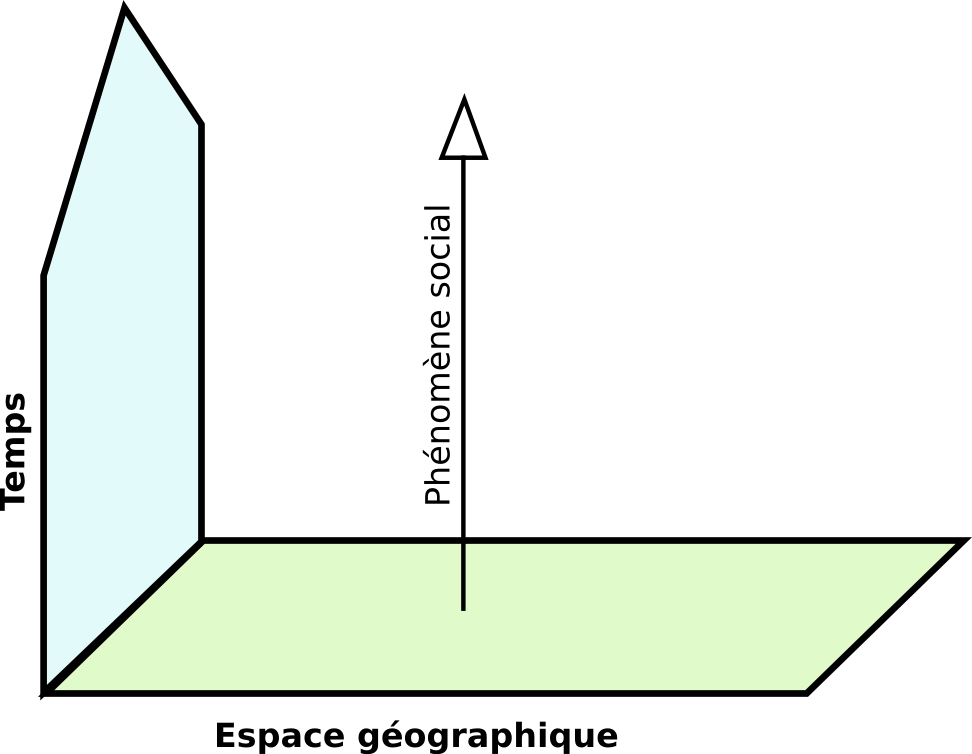
\includegraphics[width=0.2\textwidth]{spaceuse1.png} &  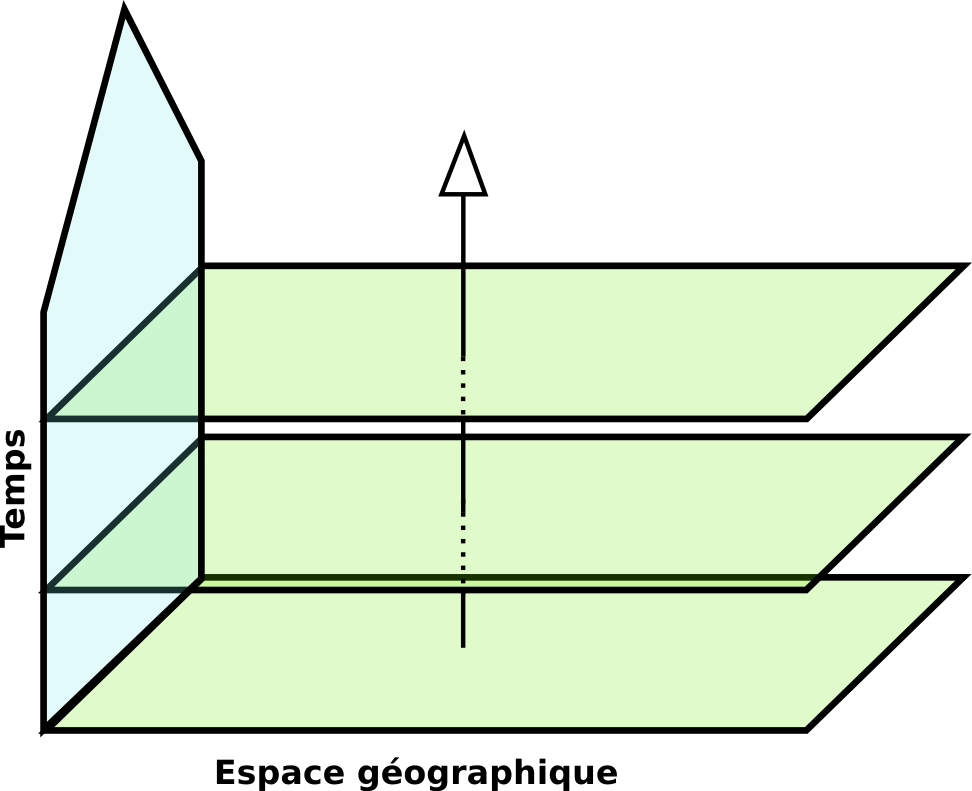
\includegraphics[width=0.2\textwidth]{spaceuse2.png} &  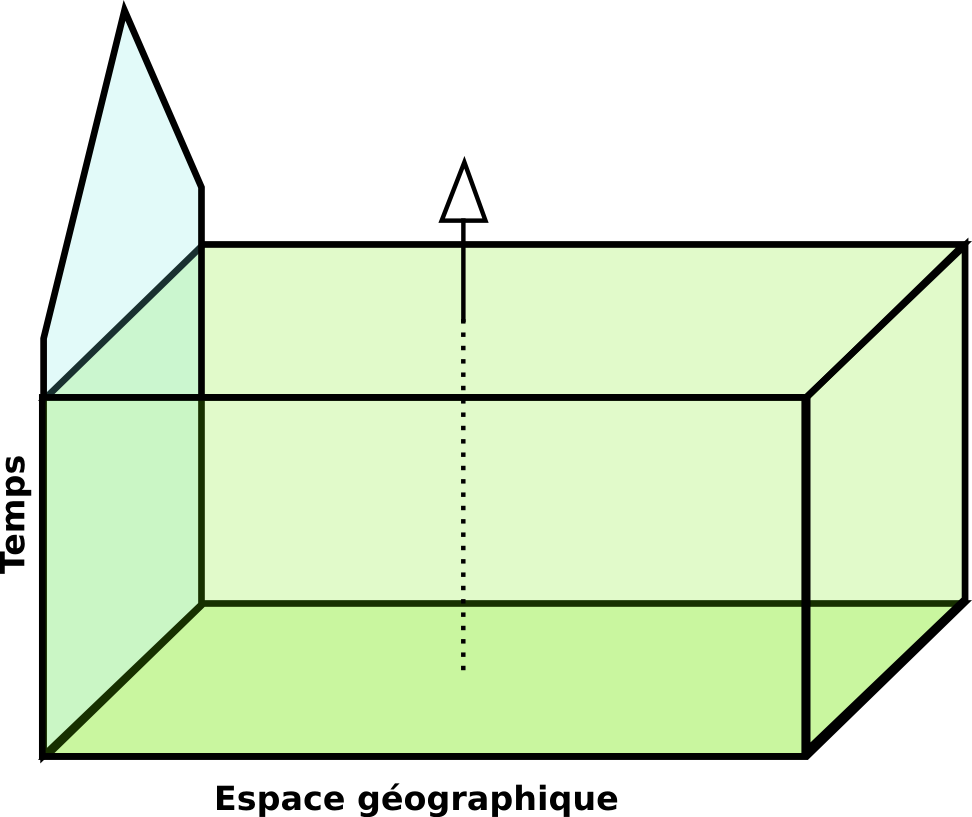
\includegraphics[width=0.2\textwidth]{spaceuse3.png} \tabularnewline
\hline
\textbf{Abstraction spatiale} &  +++ & + &  + \tabularnewline
\hline
\textbf{�chelle}\footnote{D'apr�s \cite{Ruas1999}.}  & \textbf{macro} (ensemble de villes, pays, etc.) & \textbf{m�so} (ville) & \textbf{m�so ou micro} (quartier, b�timent,etc.) \tabularnewline
\hline
\textbf{Dimensions} & \textcolor{cyan}{\textbf{T}} & \textcolor{green}{\textbf{S}}+\textcolor{cyan}{\textbf{T}} & \textcolor{magenta}{\textbf{ST}} \tabularnewline
\hline
\end{tabular}
\end{center}
\end{table}


\subsection{Conclusion~: besoins g�n�raux}
Les 3 cat�gories d'int�gration du temps dans l'�tude de l'espace urbain ne sont finalement pas isol�es les unes des autres, mais r�sultent d'une gradation de l'insertion de l'espace urbain dans le temps.
De cette imbrication na�t la relation entre l'espace et des ph�nom�nes sociaux particuliers~; c'est consid�rer que l'espace de la ville permet de mieux comprendre les ph�nom�nes sociaux qui s'y sont d�roul�s parce qu'il influe sur ces activit�s et qu'il en porte les traces r�siduelles.
Un tel gradient fait �cho � la volont� de Roncayolo, illustr�e par \cite{Walter2005}, d'�tudier la ville en effectuant une \emph{r�duction au temps} de la m�me mani�re que \cite{Braudel1951} plaidait pour une \emph{r�duction � l'espace}.
\subparagraph{}
Spatialiser des information sociales se concr�tise la plupart du temps au travers de la production de cartes~\citep[p. 102-103]{Arnaud2008}.
Manipuler l'espace ancien signifie donc le repr�senter~: mentalement d'abord, mais aussi visuellement par la 
construction de cartes, la mise en commun et le croisement de sources historiques.
De cet int�r�t pour la construction de repr�sentations du pass�, on peut d�gager trois besoins particuliers~:
\begin{enumerate}
\item \textbf{Localiser des donn�es sociales} d�crivant un des ph�nom�nes ou des faits sociaux, dans l'espace urbain \textbf{contemporain} de leur �poque.
Abstrait, l'espace reste le contexte de l'�tude mais il permet d'expliquer certaines sp�cificit�s d'un ph�nom�ne par sa localisation g�n�rale (par exemple les particularit�s du cosmopolitisme dans les villes c�ti�res chez \cite{Lafi2011}).
Lorsqu'il est plus concret, l'espace permet de situer les donn�es sociales et de faire appara�tre des motifs d'organisations des individus, des jeux de pouvoirs qui se traduisent dans la r�partition des individus, des �v�nements, etc.
\item \textbf{Repr�senter l'organisation des structures de l'espace et ses transformations au cours du temps}, dans le but de faire appara�tre des motifs, des brisures ou � l'inverse des zones de r�siliences de l'espace.
\item \textbf{Repr�senter l'�volution conjointe de l'espace et d'un ph�nom�ne social qui s'y d�roule}.
Il s'agit d'un besoin li� au niveau de relation espace/temps le plus fort, dans lequel les relations de r�troaction entre l'espace urbain et les activit�s sociales sont directement consid�r�es au sein de l'�tude.
\end{enumerate}
Plus dynamiques spatiales et sociales sont m�l�es, plus il devient important de reconstituer les �tats et les transformations de l'espace afin d'en produire une repr�sentation visuelle.
La complexit� de ces transformations et le niveau de d�tail demand� par de tels travaux impliquent une connaissance fine de l'espace �tudi� ne pouvant �tre acquise qu'au travers des traces qu'il faut rassembler et lier au sein d'une repr�sentation visuelle coh�rente.
%
%\begin{center}
%\fcolorbox{black}{white}{
%  \begin{minipage}[t]{0.9\textwidth}
%\begin{center}
% \textbf{R�sum� de la section}
%\end{center}
%L'espace de la ville est abord� de fa�ons diverses selon les objectifs des �tudes historiques et selon les angles de vues qu'elles adoptent. Plus encore, c'est le degr� de consid�ration pour les interactions entre l'espace g�ographique et les ph�nom�nes sociaux qui va conditionner la place prise par l'espace urbain dans l'�tude. � partir d'un statut pratiquement neutre, d�corell� du temps et plac� comme une toile de fond sur laquelle se dessine un ph�nom�ne social, l'espace prend peu � peu une place centrale dans l'�tude historique. D'abord trait� comme un outil permettant, par la localisation dans l'espace des donn�es sociales, de mieux comprendre un ph�nom�ne et de faire appara�tre de nouvelles questions historiques, il est finalement compl�tement int�gr� dans le temps et consid�r� dans ses interactions avec les ph�nom�nes sociaux.
%\subparagraph{}
%Nous explicitons cette gradation au travers d'une �chelle constitu�e de trois niveaux li�s les uns aux autres. Chaque niveau est illustr� par des exemples issus de travaux r�cents en histoire portant sur des villes. La description de cette �chelle nous permet finalement de dresser une liste de trois demandes fondamentales d'un travail historique portant sur un espace urbain : la spatialisation de donn�es sociales, la repr�sentation visuelle d'un espace ancien et enfin la repr�sentation de ses transformations au cours du temps. Pour chaque besoin, la repr�sentation de l'espace prend une part importante de la demande. 
%  \end{minipage}
%} 
%\end{center}


\section{Repr�senter un espace urbain en transformation}
\label{section:carto_ancienne}
\myparagraph{Repr�sentation cartographique de l'espace}
Nous avons pr�sent� la demande d'une repr�sentation repr�sentation de l'espace pass� pour l'histoire urbaine.
Il peut en effet sembler naturel qu'un travail sur l'espace implique la production de repr�sentations visuelles de celui-ci, notamment cartographiques, �tant donn� la force du lien ainsi cr�� avec la g�ographie.
La repr�sentation de l'espace, comme le fait remarquer \cite{Palsky2004}, est une notion relativement complexe et surtout doublement connot�e~: c'est � la fois le processus de cr�ation d'une image mentale mais aussi l'image elle-m�me.
La carte est une concr�tisation de cette repr�sentation sous forme d'image stabilis�e, c'est \emph{une abstraction de la r�alit� spatiale [...] mod�lis�e et cod�e afin d'�tre appr�hend�e par le regard.}
\subparagraph{}
Lorsqu'il s'agit de repr�senter un espace pass�, le processus de repr�sentation cartographique peut intervenir � deux moments distincts.
En effet, l'espace dont on souhaite produire une repr�sentation n'existe plus et n'est donc plus accessible � l'observation directe.
En cons�quence, il doit d'abord faire l'objet d'une reconstruction � partir des traces qui se sont d�cant�es au cours du temps\footnote{Une trace est la marque d'un objet ou d'un �v�nement dont la particularit� est \emph{d'avoir �t�}.
Une trace cr�e donc syst�matiquement un d�calage entre le moment de sa cr�ation et sa lecture, d�calage pendant lequel elle peut se d�composer ou se d�sint�grer\cite{Kramer2012}.
Les restants d'un ancien mur, un r�cit de voyage ou un portulan sont autant d'exemples de traces d'un espace pass�.}.
C'est ce point pr�cis�ment que nous allons d�velopper par la suite dans la section \ref{subsection:sources}.
Une fois cette repr�sentation construite, elle peut servir de base � l'analyse ou d'outil permettant de localiser des informations diverses.
� partir du moment o� l'on dispose d'une repr�sentation visuelle d'un espace ancien, elle peut servir � la communication des r�sultats du travail ou bien de contexte visuel pour la repr�sentation et l'interpr�tation de donn�es sociales.
C'est donc un processus en deux temps qui s'impose lorsqu'il s'agit de travailler sur une configuration spatiale pass�e.
Nous proposons d�s lors d'analyser plus avant ce processus pour en identifier les complexit�s, en pr�sentant d'abord les diff�rents types de traces consid�r�es sur l'espace.
Nous nous concentrerons dans la section \ref{subsection:plans} sur les sources cartographiques, qui par leur nature se pr�tent le plus naturellement � la construction de repr�sentations visuelles de l'espace.

\myparagraph{La recherche de traces}
Dans son livre \emph{History and GIS}, \cite{Lunen2013} fait le parall�le, � titre illustratif, entre le travail d'un historien et ceux d'un enqu�teur ou d'un chasseur.
L� o� l'enqu�teur cherche des pi�ces � conviction lui permettant d'�tablir la culpabilit� ou l'innocence d'un accus�, ou encore de chercher le coupable d'un crime, l'historien cherche au sein d'archives les �l�ments lui permettant de r�pondre � une question historique, de retracer les faits, les �v�nements et leur contexte historique.
L�nen note cependant que les m�thodes sont radicalement diff�rentes.
� la diff�rence de l'enqu�teur qui se base sur des proc�d�s de d�ductions lui permettant de recomposer une sc�ne de crime, l'historien proc�de par abduction, c'est � dire par la formulation d'une hypoth�se historique qu'il va tenter de faire appara�tre au travers de l'agencement des traces historiques qu'il a � sa disposition.
\subparagraph{}
Cette analogie peut sembler grossi�re, mais elle met assez bien en �vidence la fa�on de proc�der d'un historien~: � partir d'une question historique pr�cise, il va chercher des faits tangibles lui permettant d'y r�pondre.
Il trouve dans le particulier des �l�ments lui permettant, par g�n�ralisation, de r�pondre � une question plus large.
Lorsque cette question est profond�ment spatiale, ou bien que l'historien fait l'hypoth�se que l'espace y joue un r�le, le travail historique passe par la mise en relation de traces spatiales ou spatialisables issues de sources historiques diverses.
\subparagraph{}
Au del� m�me des traces directement lisibles au sein de sources historiques, leur croisement permet de faire appara�tre de nouvelles informations.
Par exemple, la comparaison de deux cartes d'un quartier � des �poques diff�rentes peut permettre d'acqu�rir des connaissances sur la fa�on dont le quartier s'est transform�.
Du fait de l'importance de ce travail de recherche de traces, de croisement et d'extraction de connaissances nouvelles, il est crucial de garder en t�te ses particularit�s lors de la cr�ation d'outils et de mod�les SIG adapt�s au travail historique.

\myparagraph{Recomposer n'est pas r�pliquer}
Lorsque l'on cr�e une repr�sentation d'un espace ancien, il ne n'agit pas d'essayer de reproduire la r�alit� � un temps donn�, d'autant plus qu'il est impossible d'appr�hender une r�alit� complexe.
Cet �tat de fait est largement admis dans les sciences sociales, mais �galement parmi les disciplines traitant de l'information (g�ographique notamment) \citep{Bodenhamer2010}.
Pour la g�omatique en particulier, cette question se trouve � la source des mod�les de qualit� des donn�es et d'imperfections de l'information spatiale \citep{Leyk2005}.
L'historien, lui, manipule des sources -des traces- dont il conna�t les d�fauts et dont il questionne syst�matiquement la fiabilit�.
Il faut s'interroger �galement sur la capacit� des SIG � g�rer de telles sources et � manipuler des informations dont la fiabilit� est tr�s variable.
%L'impr�cision des traces et de l'information spatiale qu'elles contiennent se trouve d'une recomposition pertinente d'un espace pass� et de ses dynamiques.

\subsection{Information g�ohistorique}
\label{subsection:info_geohisto}
Dans le domaine des syst�mes d'informations g�ographiques, on d�signe par ''information g�ographique'' le couple form� d'une information portant sur un objet ou un ph�nom�ne du monde terrestre et d'une localisation � la surface de la Terre dans un syst�me de r�f�rence explicite \citep{Denegre1996}.
La perception de cette information g�ographique est classiquement consid�r�e comme le fait de structurer l'espace r�el sous la forme d'entit�s, correspondant � un ph�nom�ne quelconque du monde r�el (une personne, un b�timent, l'Europe, un champs de bataille, etc.) \citep{Plewe2002}.
Le champ de bataille et la personne sont pourtant des entit�s tr�s diff�rentes.
Leurs limites en particulier n'ont rien de comparable.
Dans le cas d'une personne, � l'�chelle macroscopique du moins, sa limite est �tablie \emph{de facto}.
Il en va d'une mani�re tout � fait diff�rente pour le champs de bataille~: ses limites r�sultent de processus cognitifs plus complexes.


\myparagraph{Entit�s}
\label{paragraph:entite}
Cette diff�rence entre entit�s g�ographiques a �t� formalis�e par \cite{Smith1995}.
Il classifie ainsi ces diff�rentes entit�s en deux groupes de natures  diff�rentes~:
\begin{itemize}
 \item Les entit�s \emph{bona fide} pr�sentent des limites directement perceptibles.
� une �chelle macroscopique tout du moins, une personne ou une �le sont des entit�s \emph{bona fide}.
Leurs limites sont clairement visibles et la correspondance entre l'objet du monde r�el ''personne'' ou ''�le'' et sa repr�sentation cognitive est directe.
 \item Les entit�s \emph{fiat} sont au contraire des entit�s dont les limites sont cr��es de toutes pi�ces par l'Homme.
Un pays, une paroisse en sont des exemples~: leurs limites peuvent localement s'appuyer sur des �l�ments naturels, mais elles restent des constructions humaines.
\end{itemize}
\cite{Plewe1997} ajoute un troisi�me groupe qu'il nomme \emph{motivated entities}.
Comme les entit�s \emph{fiat}, leurs limites n'existent pas de fa�on concr�te dans la r�alit�, mais cette fois elles r�sultent de processus cognitifs plus ou moins complexes tels l'agr�gation, la cat�gorisation ou la simplification.
La ville est clairement une entit� motiv�e.
Les d�limitations d'une ville proc�dent de regroupements de structures humaines dont la densit� ou l'organisation d�finissent une certaine notion d'urbanit�.
\subparagraph{}
\cite{Smith2010} font cependant remarquer que la s�paration entre entit�s \emph{fiat} et \emph{bona fide} n'est pas si �vidente~: les limites d'une entit� peuvent �tre m�lang�es.
Ainsi, les quartiers parisiens actuels sont des entit�s \emph{bona fide} dont les contours sont d�finis par des rues ou la Seine, mais qui sont �galement des constructions humaines sans existence \emph{de facto}.
Les entit�s sont alors moins d�finies par leurs fronti�res seules que par opposition � d'autres entit�s.
Nous pensons que la m�me critique peut �tre faite pour les entit�s motiv�es.
Les faubourgs anciens de Paris se d�finissent dans leur rapport d'opposition avec la ville elle-m�me.


\myparagraph{Temps, s�mantique, espace}
Les entit�s g�ographiques sont d�finies non seulement dans l'espace, mais �galement dans le temps, et sont associ�es � une s�mantique particuli�re \citep{Plewe2002}~: chaque entit� \emph{existe � un endroit donn�, pendant une p�riode donn�e et poss�de des propri�t�s particuli�res}.
Ces trois �l�ments d�finissent les trois dimensions d'une entit� g�ographique~: \textbf{sa localisation et sa forme, sa p�riode de vie et ses attributs}.
Ces trois �l�ments forment alors l'�tendue de l'entit� g�ographique.
Par exemple, la rue \emph{Au Maire}, situ�e dans le 3\up{�me} arrondissement de Paris existe depuis 1280 \citep{Lazare1844}.
L'entit� g�ographique correspondante peut �tre alors constitu�e de la forme de la rue, sa p�riode de vie �tant l'intervalle ouvert [1280;2013[, et sa description peut �tre son nom (la figure \ref{fig:aumaire} donne un aper�u des transformations de la rue Au Maire).
\subparagraph{}
Cette triple consid�ration (s�mantique, spatiale et temporelle) est pr�sente depuis longtemps dans le domaine de la g�ographie \citep{Berry1964,Sinton1978, Hagerstrand1970}, mais les SIG se sont form�s sur le mod�le d'une information atemporelle \citep{Goodchild2008}.
C'est pourtant cette information triple qu'il est crucial de manipuler pour repr�senter un ph�nom�ne historique, que nous d�signerons dans l'ensemble de ce document comme \textbf{g�ohistorique}\citep{Plewe2002}.
L'information g�ohistorique n'est donc pas oppos�e � l'information g�ographique, mais pr�cise seulement le fait qu'elle traite d'entit�s spatiales disparues ou ayant une �paisseur temporelle donn�e.
\begin{figure}[ht]
  \centering
  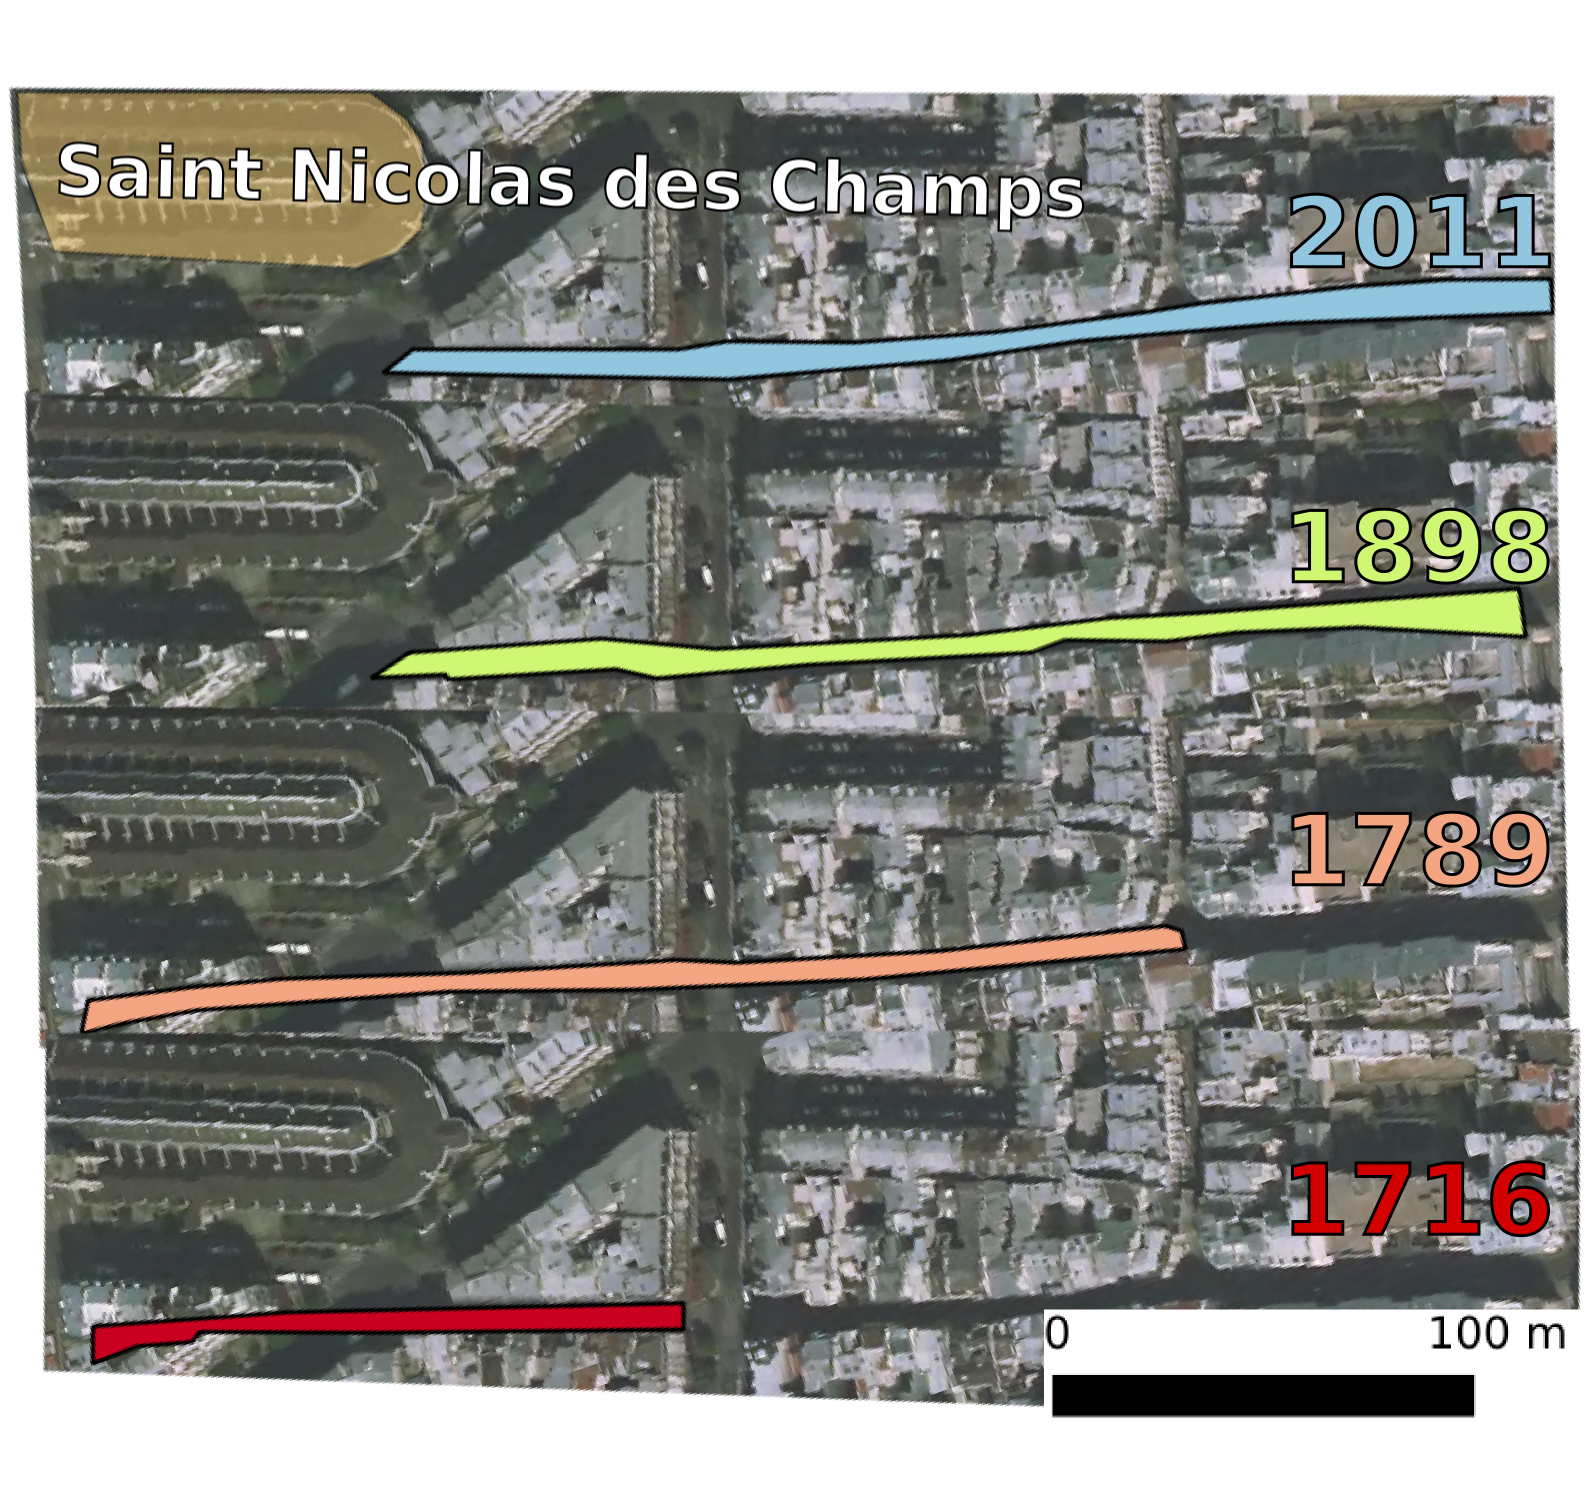
\includegraphics[width=0.50\textwidth]{aumaire_echelle.png}
  \caption{Les transformations de la rue actuelle \emph{Au Maire} comme d�crite par des plans successifs de 1716 � nos jours.
L'�glise Saint Nicolas des Champs, au sud du Conservatoire National des Arts et M�tiers, sert de rep�re.}
  \label{fig:aumaire}
\end{figure}



\myparagraph{Identit�}
Une quatri�me dimension doit �tre ajout�e � cette d�finition.
En effet, l'identification d'un objet g�ographique du monde r�el repose sur la possibilit� de lui attribuer une existence qui le d�finit de fa�on univoque.
Cette identit� est d�finie ind�pendamment des trois autres dimensions.
L'identification claire d'une entit� est une question complexe, notamment pour les donn�es spatio-temporelles \citep{DelMondo2011}.
Si l'on reprend le cas de la rue \emph{Au Maire}, la d�finition de son identit� n'est pas triviale.
En effet, la rue a �t� consid�rablement allong�e en 1833\footnote{\href{[http://www.v2asp.paris.fr/commun/v2asp/v2/nomenclature_voies/Voieactu/5856.nom.htm}{Index des rues fourni par la ville de Paris.}}, englobant le trac� d'un ancien \emph{Cul de Sac de Rome}.
D�s lors, la rue \emph{Au Maire} avant allongement est-elle la m�me entit� qu'apr�s? Car si le nom reste inchang�, le trac� n'est plus le m�me.

\subparagraph{}
L'affectation d'une identit� � des entit�s g�ographiques pose d'importants probl�mes lorsque l'on manipule des objets spatio-temporels.
En effet, si la rue \emph{Au Maire} conserve son identit� malgr� les travaux, il s'agit toujours du m�me objet qui se transforme.
Mais si l'on consid�re que par cette op�ration c'est une nouvelle rue qui est cr��e, alors la question est toute diff�rente, puisqu'il s'agit cette fois d'une entit� qui dispara�t au profit d'une autre, il n'y a plus transformation mais brisure.
Puisqu'il s'agit dans cette th�se de traiter d'entit�s g�ohistoriques et donc spatio-temporelles, cette question se verra approfondie dans les chapitres 5 et 6.


\subsection{Typologie des sources d'information historiques sur l'espace urbain}
\label{subsection:sources}
Puisqu'il s'agit d'espaces disparus, il n'est plus possible d'en obtenir une repr�sentation par l'observation directe et celle-ci doit �tre reconstitu�e � partir des informations g�ohistoriques qui subsistent au travers de sources diff�rentes, documents cr��s par les contemporains ou traces arch�ologiques \footnote{Une source ou document historique est [...] toute trace, tout indice de la pr�sence, de l'activit�, de la mentalit� de l'Homme d'autrefois~\citep{Godding1999}}.
Ainsi, une carte topographique ancienne, un recensement comprenant les adresses postales des individus, ou les bornes de d�limitation d'une ancienne censive constituent autant de ces ressources que l'on nomme ici \textbf{sources g�ohistoriques}.
Si elles sont le mat�riel essentiel d'une �tude de la ville, elles constituent un ensemble fortement h�t�rog�ne en raison de leur diff�rences, mais �galement de biais issus des partis pris et objectifs de leurs auteurs \citep{Knowles2008}.
\subparagraph{}
Nous proposons ici de mettre en place une typologie de ces sources g�ohistoriques afin d'en expliciter les sp�cificit�s en termes de modes de repr�sentation de l'espace mais �galement de biais.
Il n'existe pas de classification unique de ces sources, mais il est possible de produire une synth�se des propositions apparaissant dans divers ouvrages.
Nous nous fondons ici sur deux typologies en particulier qui pr�sentent l'avantage de se compl�ter.
\subparagraph{}
D'abord, on peut effectuer une premi�re distinction � partir de celle �tablie par \cite{Barzun1985}, formant deux cat�gories de sources~:
\begin{itemize}
 \item \textbf{Enregistrements}~: Il s'agit des sources qui fournissent une information spatiale intentionnellement, de fa�on plus ou moins explicite.
On retrouve dans cette cat�gorie l'ensemble des documents d'archives portant des informations spatialis�es.
 \item \textbf{Reliques}~: Il s'agit des sources fournissant une information sur un espace pass� de fa�on non intentionnelle.
Il s'agit ici des artefacts arch�ologiques, mais �galement des formes urbaines persistantes ou des �l�ments architecturaux de l'espace pr�sent.
\end{itemize}
Ensuite, \cite{Arnaud2008} tout comme \cite{Laurent1979} effectuent une distinction au sein des sources d'archives entre celles qui fournissent une information spatiale directement repr�sent�e et celles dont la localisation doit �tre retrouv�e (par exemple, les adresses d'individus).
Le sch�ma \ref{fig:schema_sources} organise ainsi les diff�rents types de sources g�ohistoriques permettant de d�crire l'espace urbain ancien, chaque type �tant d�crit plus en d�tail de fa�on � souligner ses complexit�s intrins�ques.
\begin{figure}[ht]
	\centering
		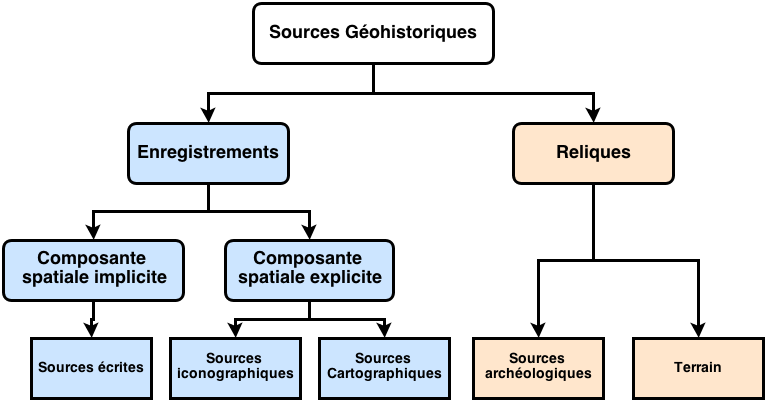
\includegraphics[width=0.8\textwidth]{typologie_sources.png}
	\caption{Typologie des sources d'informations g�ohistoriques sur l'espace urbain ancien}
	\label{fig:schema_sources}
\end{figure}


\myparagraph{Les sources cartographiques}
Lorsque l'on se concentre sur la ville, les sources cartographiques anciennes deviennent les sources d'information principales car elles permettent de localiser l'information issue d'autres sources sans composante spatiale explicite.
Par exemple, un plan parcellaire portant les num�ros des immeubles permet de localiser des individus dont l'adresse est indiqu�e dans une source textuelle (un bottin ou un recensement par exemple).
\subparagraph{}
Une source cartographique est qualifi�e d'historique d�s lors qu'elle est situ�e suffisamment loin dans le pass� pour repr�senter des transformations significatives pour une �tude donn�e.
Il s'agit donc d'une qualification subjective li�e au contexte de chaque �tude \citep{Leyk2005}.
\subparagraph{}
Les repr�sentations de l'espace urbain varient fortement et d�pendent de l'�volution des visions de la ville par les auteurs des cartes \citep{Arnaud2008}.
� partir de la p�riode moderne, deux types de repr�sentations se succ�dent.
Le premier type correspond aux plans en perspectives, m�lant une structure g�n�rale plane enrichie de vues en �l�vation des structures urbaines o� la pr�cision g�om�trique ne constitue pas le but principal.
� partir du XVIII\up{e} si�cle le plan en perspective laisse place � des plans g�om�triques visant � d�crire la topographie de la ville et aboutissant � des vues abstraites de celle-ci.
\subparagraph{}
Ces \emph{plans de villes} fournissent une vue globale du tissu urbain ancien, souvent mat�rialis�e par la voirie, le parcellaire, le b�ti et les espaces priv�s vides (cours, jardins, champs).
Ce sont �galement des sources riches en toponymes servant de support � la localisation d'informations issues d'autres sources.
Sans dresser une liste exhaustive, on retrouve souvent dans les plans de villes les noms de rues et de places, de b�timents publics ou religieux ou encore de quartiers.
La figure \ref{fig:extrait_plans} illustre ainsi le changement entre les deux types de repr�sentations au travers de deux plans de Paris datant de la premi�re moiti� du XVIII\up{e} si�cle.
\subparagraph{}
Nous avons montr� dans les sections pr�c�dentes que l'utilisation de l'espace urbain en histoire passe g�n�ralement par l'analyse visuelle et la production de cartes sur l'espace ancien.
L'importance du r�le jou� par les sources cartographiques anciennes appara�t imm�diatement, car elles constituent souvent des repr�sentations graphiques globales de l'espace �tudi�.
Ce r�le sera pr�cis� dans la section \ref{subsection:plans}.

\begin{figure}[ht]
  \centering
        \begin{subfigure}[b]{0.3\textwidth}
                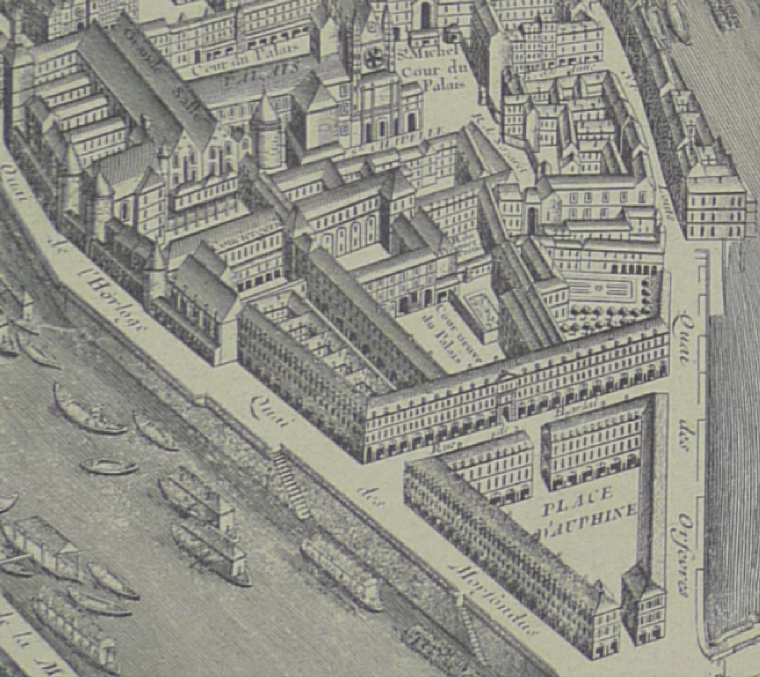
\includegraphics[width=\textwidth]{extrait_plans1.png}
                \caption{Plan de Turgot \citep{MAPTurgot}, 1739}
                \label{fig:turgot}
        \end{subfigure}%
~
	\begin{subfigure}[b]{0.3\textwidth}
                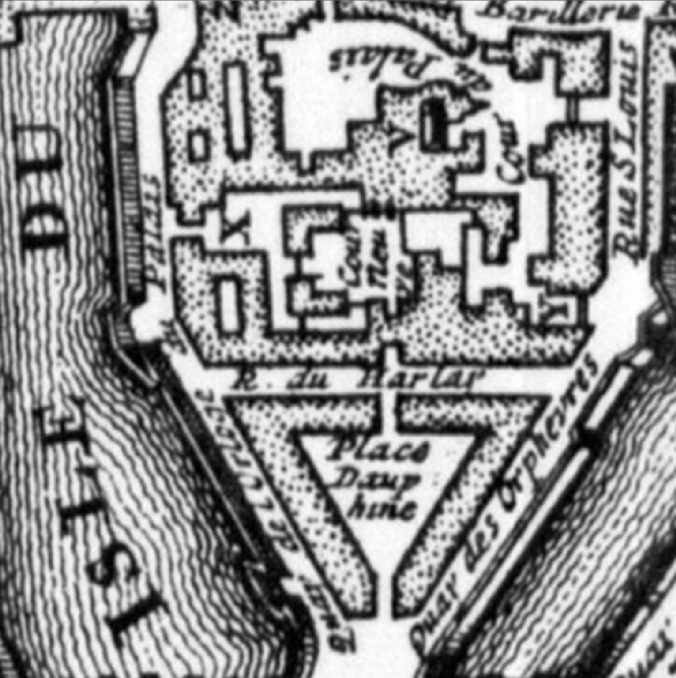
\includegraphics[width=\textwidth]{extrait_plans2.png}
                \caption{Plan de De L'isle \citep{MAPDelisle}, 1716}
                \label{fig:jaillot}
        \end{subfigure}%
         \caption{Deux visions diff�rentes du m�me espace urbain.
Extraits de plans de Paris sur l'�le de la cit�.
Les dates indiqu�es correspondent � la date de premi�re publication connue.}
	\label{fig:extrait_plans}
\end{figure}


\myparagraph{Documents �crits}
Les documents �crits constituent la ressource historique principale pour les temps les plus r�cents \footnote{Pour Paris, les documents �crits deviennent rares d�s la p�riode du moyen �ge, les historiens devant alors avoir plus largement recours aux donn�es arch�ologiques}.
Le niveau de structuration de l'information g�ohistorique varie largement au sein de cette cat�gorie.
Ainsi, il peut s'agir de textes litt�raires, juridiques, administratifs ou bien de descriptions de lieux ou de r�cits de voyages o� 
l'information g�ohistorique doit �tre interpr�t�e par l'historien afin d'�tre repr�sentable cartographiquement.
Par exemple, \cite{Eide2013} d�veloppe une m�thodologie visant � cartographier des lieux en Norv�ge d�crits de fa�on vague au sein d'un recueil de textes.
Les lieux, identifi�s par leurs noms, y sont g�n�ralement positionn�s uniquement de fa�on relative par leurs orientations et leurs distances par rapport � d'autres lieux.
\subparagraph{}
On retrouve �galement des documents dans lesquelles l'information g�ohistorique est plus structur�e et ainsi plus directement identifiable~: il s'agit de listes, annuaires, tableaux, inventaires, etc.
Ainsi, les bottins professionnels de Paris (dont un extrait appara�t dans la figure \ref{fig:bottin}) fournissent le nom, mais surtout l'adresse des travailleurs \footnote{L'adresse constitue un syst�me de r�f�rence spatial indirect \citep{Denegre1996}}, facilitant ainsi la localisation des lieux de travail.
De m�me, un inventaire apr�s d�c�s peut aider � localiser les biens immobiliers d'un individu.
Si ces documents sont fondamentaux, l'utilisation de l'information g�ohistorique qu'ils contiennent n'est pas ais�e.
En effet, elle n'est pas r�f�renc�e directement et doit donc �tre positionn�e dans l'espace par l'historien \citep{Arnaud2008}.

\begin{figure}[ht]
  \centering
        \begin{subfigure}[b]{0.32\textwidth}
                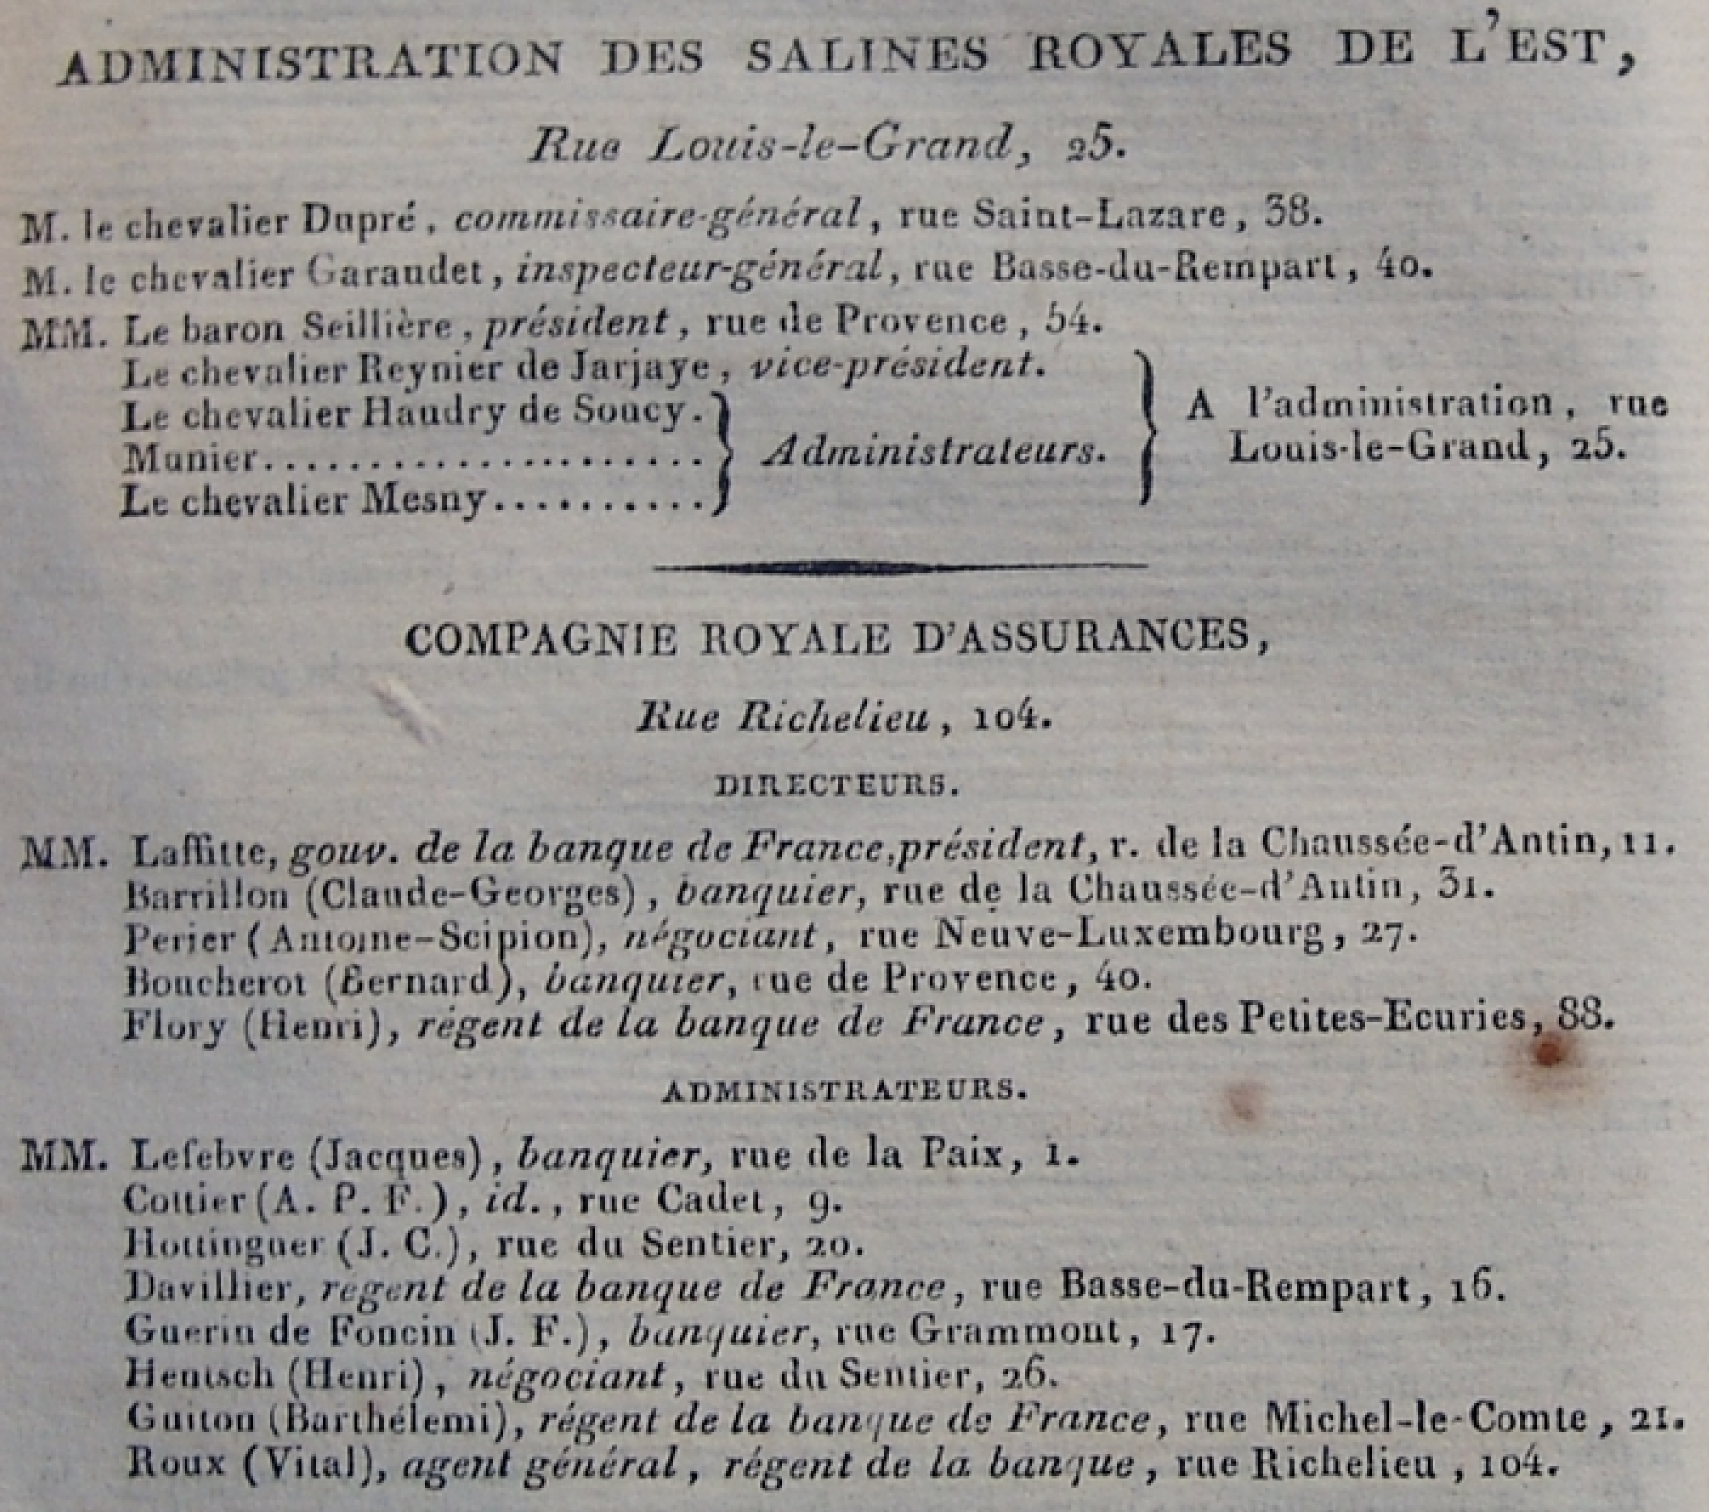
\includegraphics[width=\textwidth]{extrait_textes1.png}
                \caption{Bottin professionnel, 1818.}
                \label{fig:bottin}
        \end{subfigure}%
~
	\begin{subfigure}[b]{0.32\textwidth}
                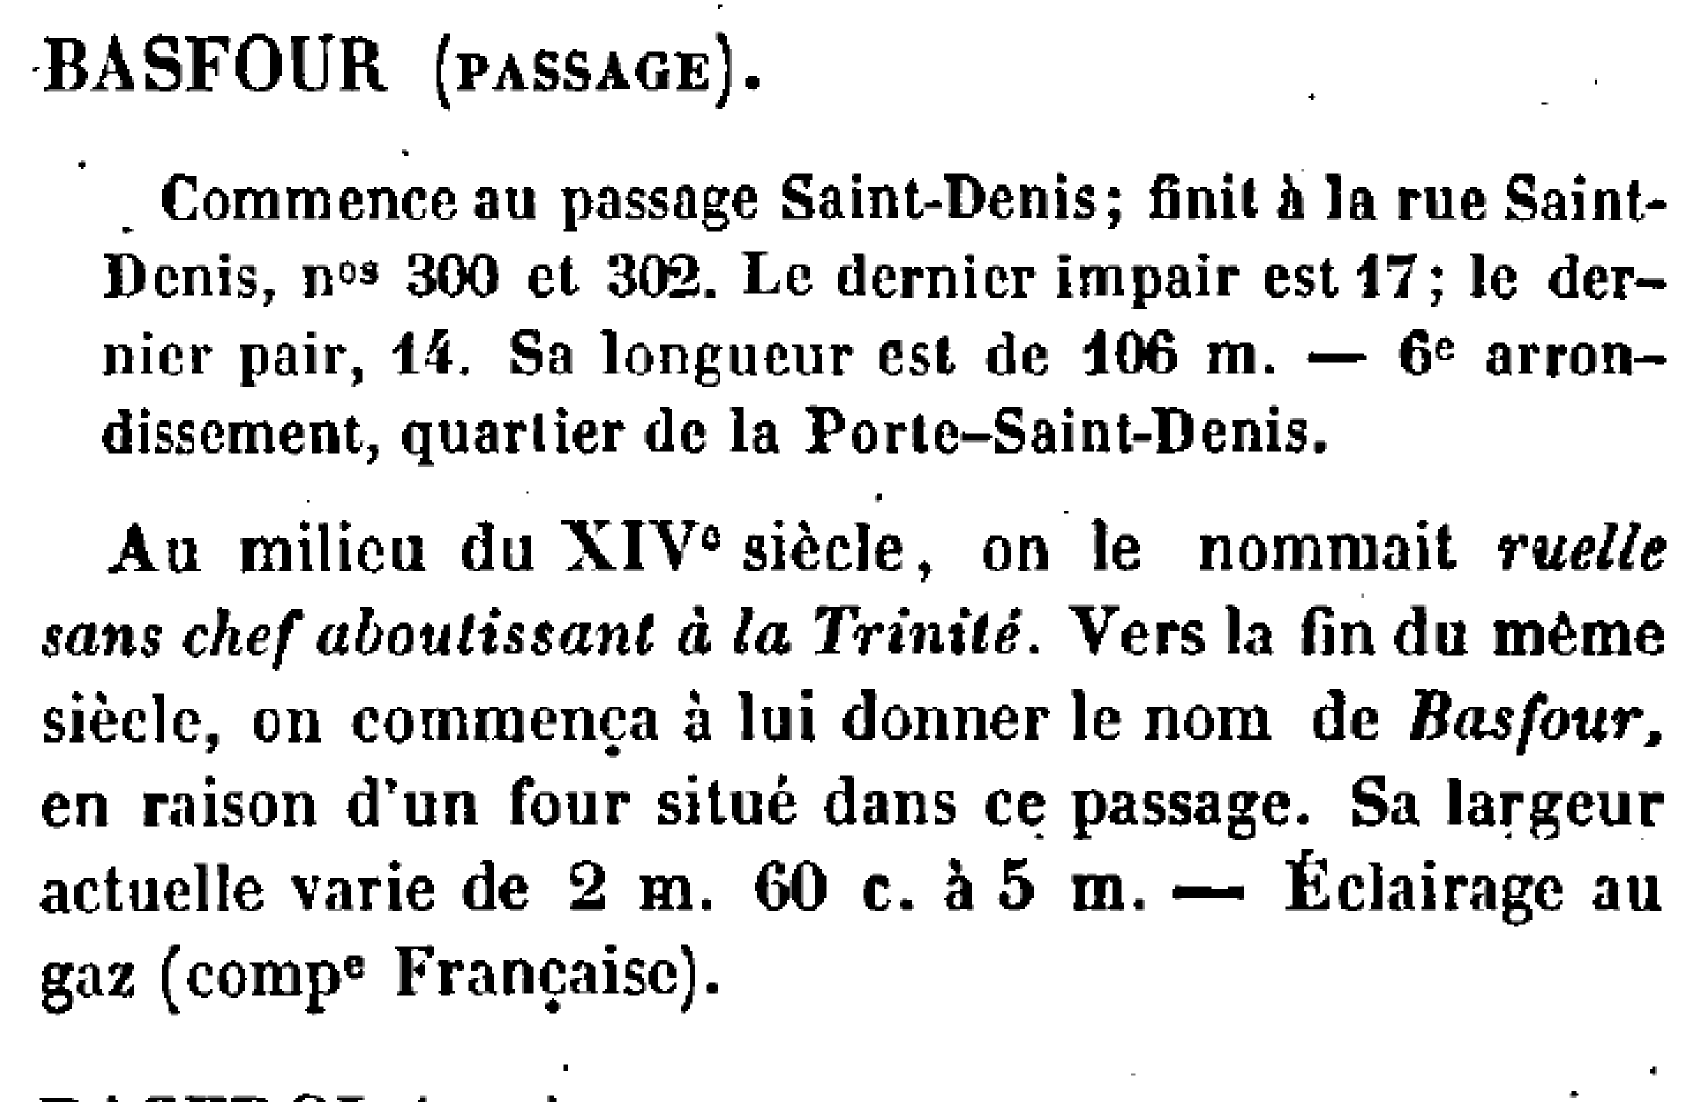
\includegraphics[width=\textwidth]{extrait_textes2.png}
                \caption{Dictionnaire des rues de Paris, 1844.}
                \label{fig:dicorues}
        \end{subfigure}%
~
	\begin{subfigure}[b]{0.32\textwidth}
                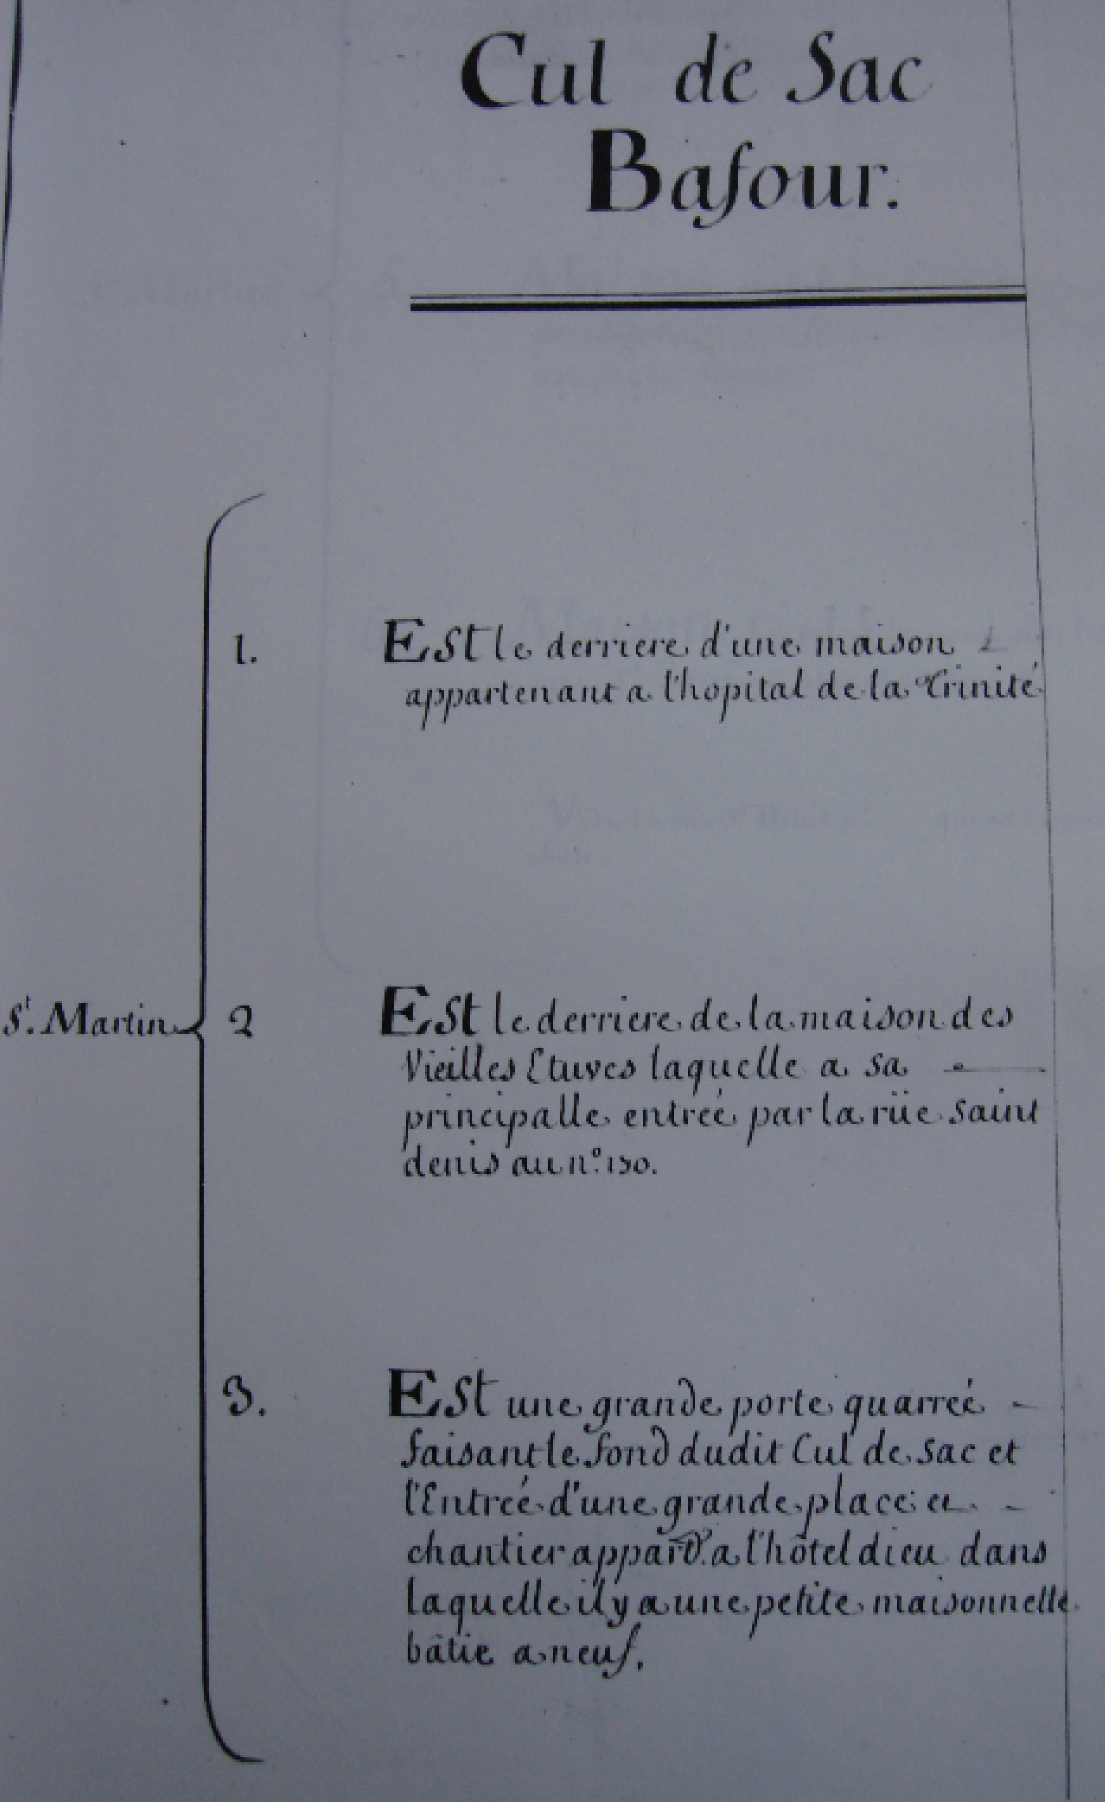
\includegraphics[width=\textwidth]{extrait_textes3.png}
                \caption{\emph{Terrier du Roy}, 1700}
                \label{fig:terrier}
        \end{subfigure}%
         \caption{Extraits de sources �crites porteuses d'informations spatiales.
Source~: LaD�His, EHESS.}
	\label{fig:textes}
\end{figure}


\myparagraph{Iconographies et photographies}
Les iconographies et photographies de la ville jouent un r�le fondamental dans la perception de l'espace urbain ancien car si elle d�crivent g�n�ralement un espace restreint, elles se placent g�n�ralement du point de vue du pi�ton pour fournir un t�moignage visuel unique de l'architecture et de l'organisation de la ville.
Les sources iconographiques forment un ensemble h�t�rog�ne de documents, en raison de l'�volution des techniques mais aussi des objectifs vari�s des auteurs.
Ainsi, les esquisses, gravures ou estampes (voir figure \ref{fig:carroussel}) fournissent � la fois des descriptions d�taill�es de l'espace d�peint, mais forment aussi un puissant vecteur de messages politiques.
La quantit� et la qualit� des estampes augmentent par exemple largement sous la R�volution Fran�aise, refl�tant ainsi leur utilisation comme outil politique � un moment o� la notion d'opinion publique prend de l'importance \citep{Bosseno1990}.
Les plans architecturaux constituent un autre ensemble o� la priorit� r�side dans la description pr�cise d'une structure b�tie.
\subparagraph{}
� partir du milieu du XIX\up{e} si�cle, l'arriv�e de la photographie apporte un t�moignage plus direct des structures urbaines (voir figure \ref{fig:marville}).
Cependant la photographie n'est pas un objet neutre, le message v�hicul� par l'auteur se transcrivant dans les choix de cadrage, les modes de prise de vue, etc.\footnote{On peut citer pour illustration le travail effectu� par \cite{Sicard1999}, notamment sur les photographies effectu�es pour le compte du baron Haussmann par Charles Marville (1813-1879).} 
\subparagraph{}
Si la richesse des ressources iconographiques permet de produire une repr�sentation d�taill�e de l'espace urbain, il s'agit d'une repr�sentation partielle et dont il est souvent difficile d'�valuer la fiabilit�.
\begin{figure}[ht]
  \centering
        \begin{subfigure}[b]{0.4\textwidth}
                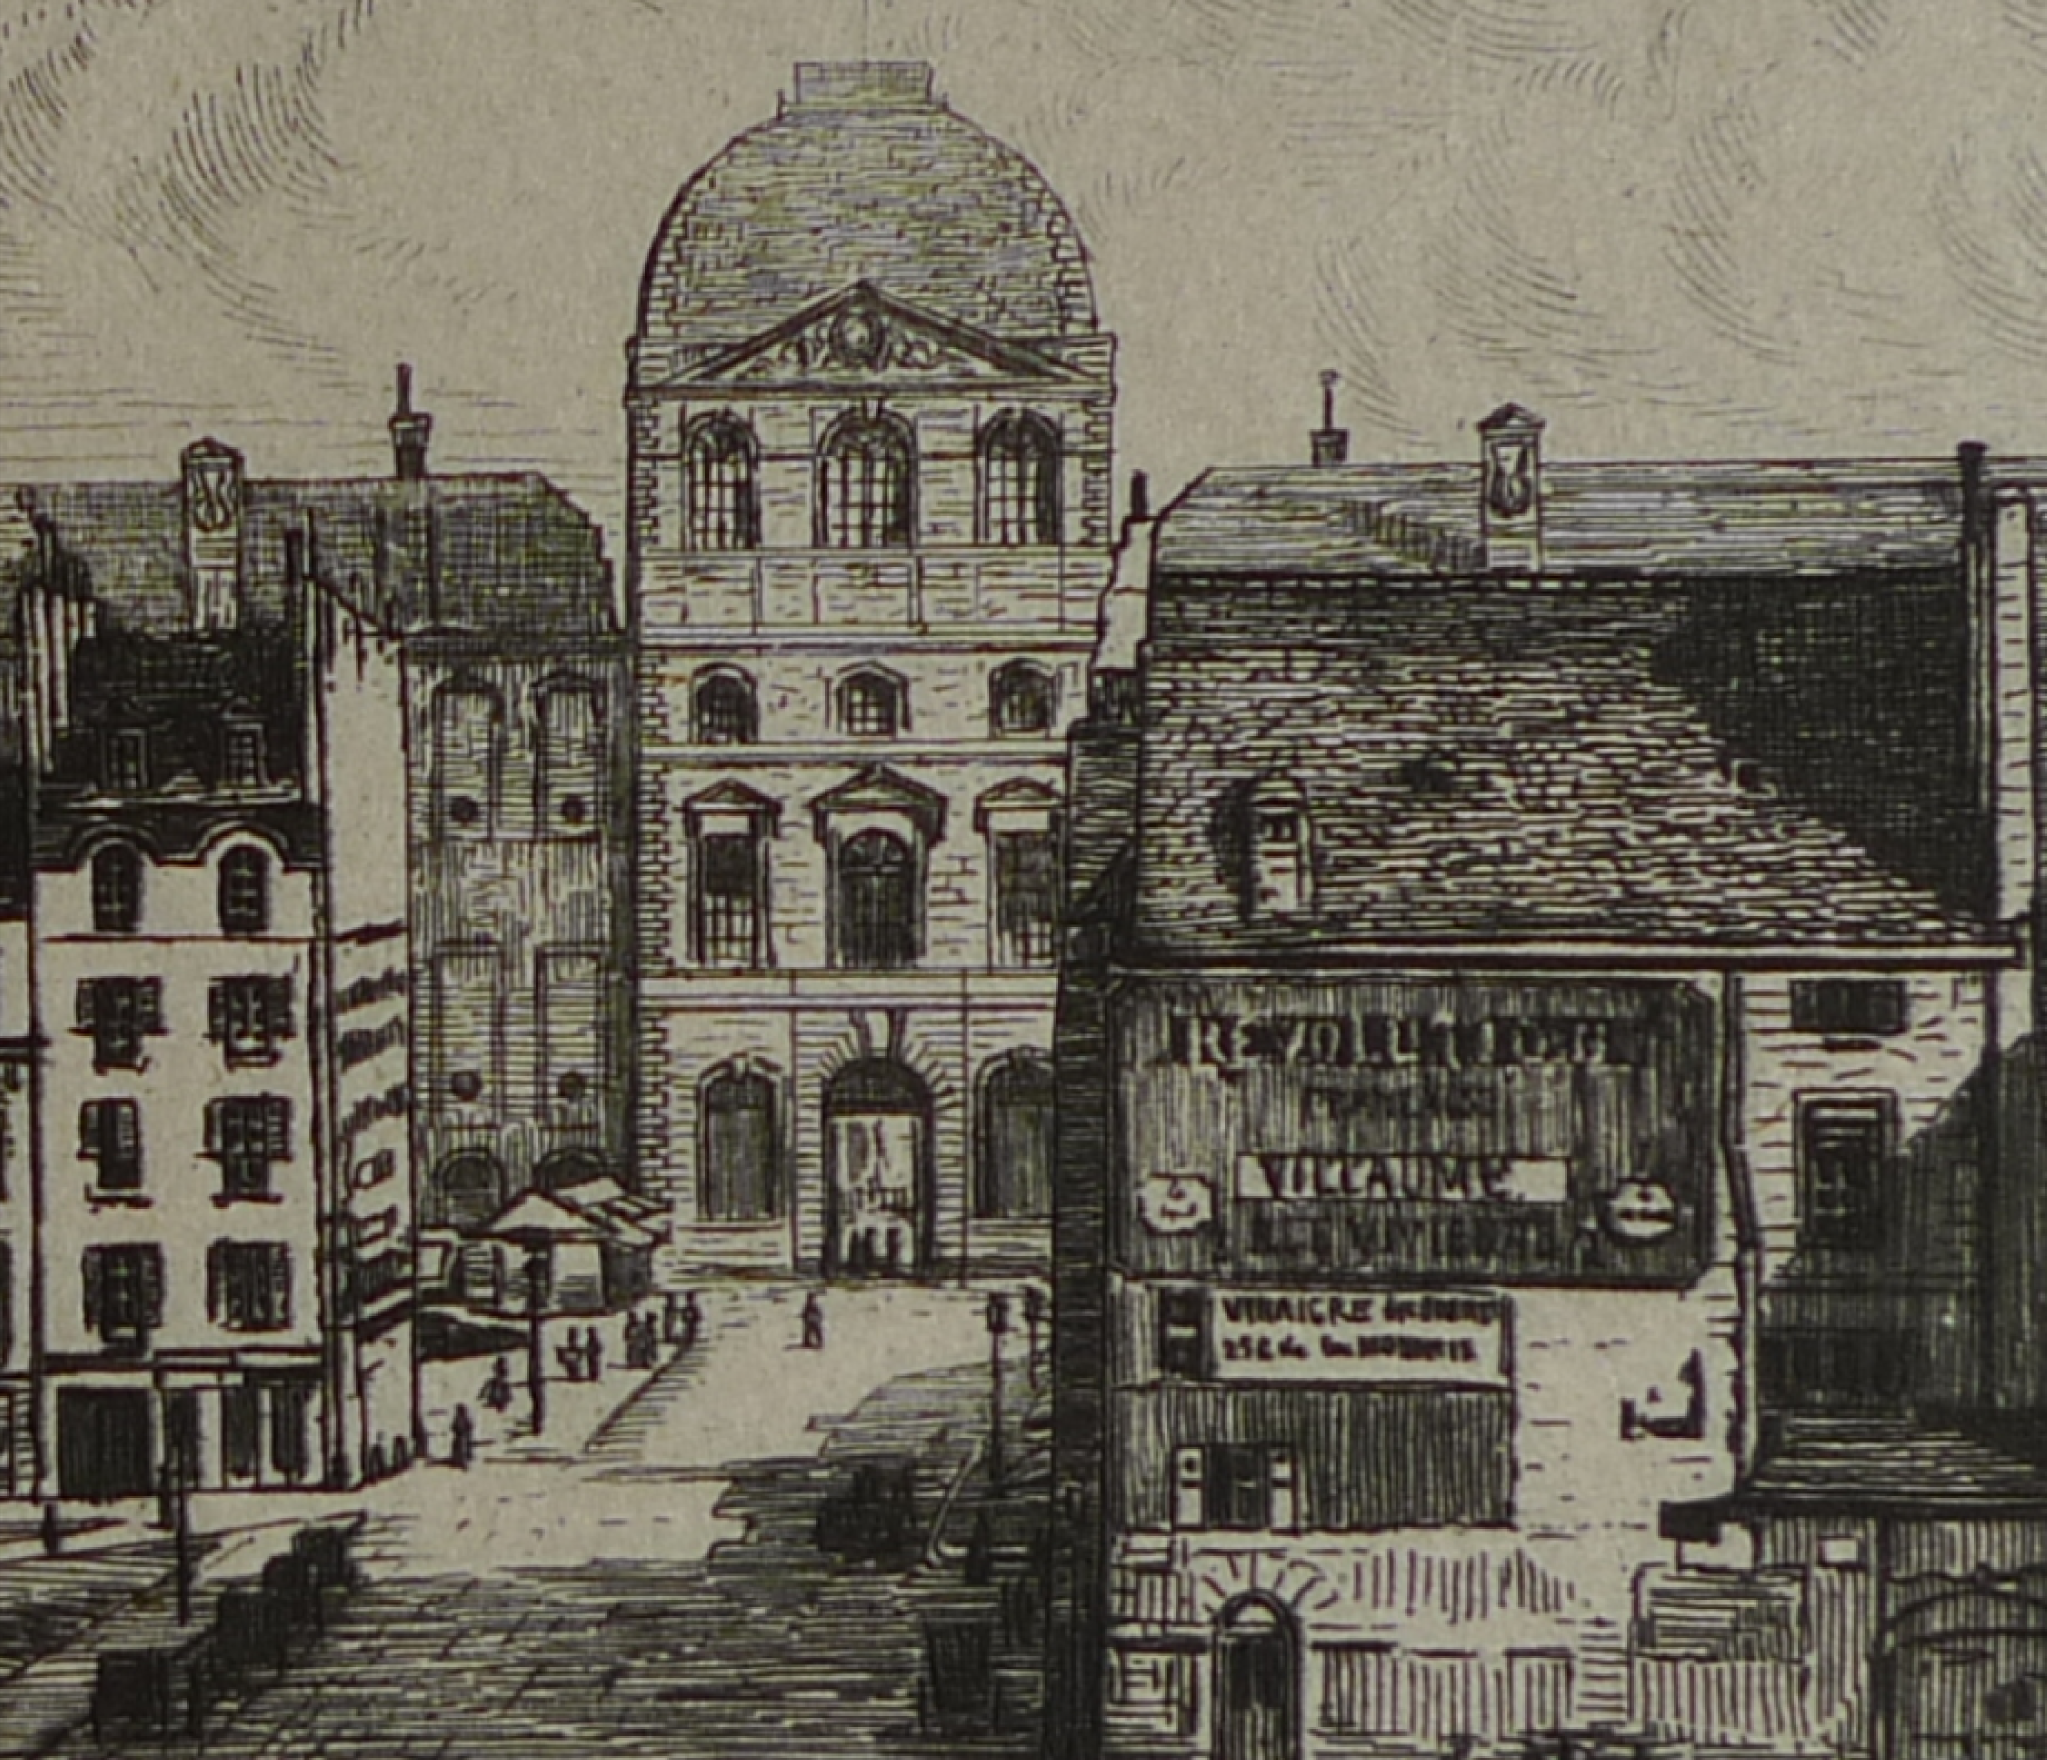
\includegraphics[width=\textwidth]{extrait_icono1.png}
                \caption{Le carroussel du Louvre, Paris, 1849}
                \label{fig:carroussel}
        \end{subfigure}%
~~~~~~~~~~~~~~~
	\begin{subfigure}[b]{0.4\textwidth}
                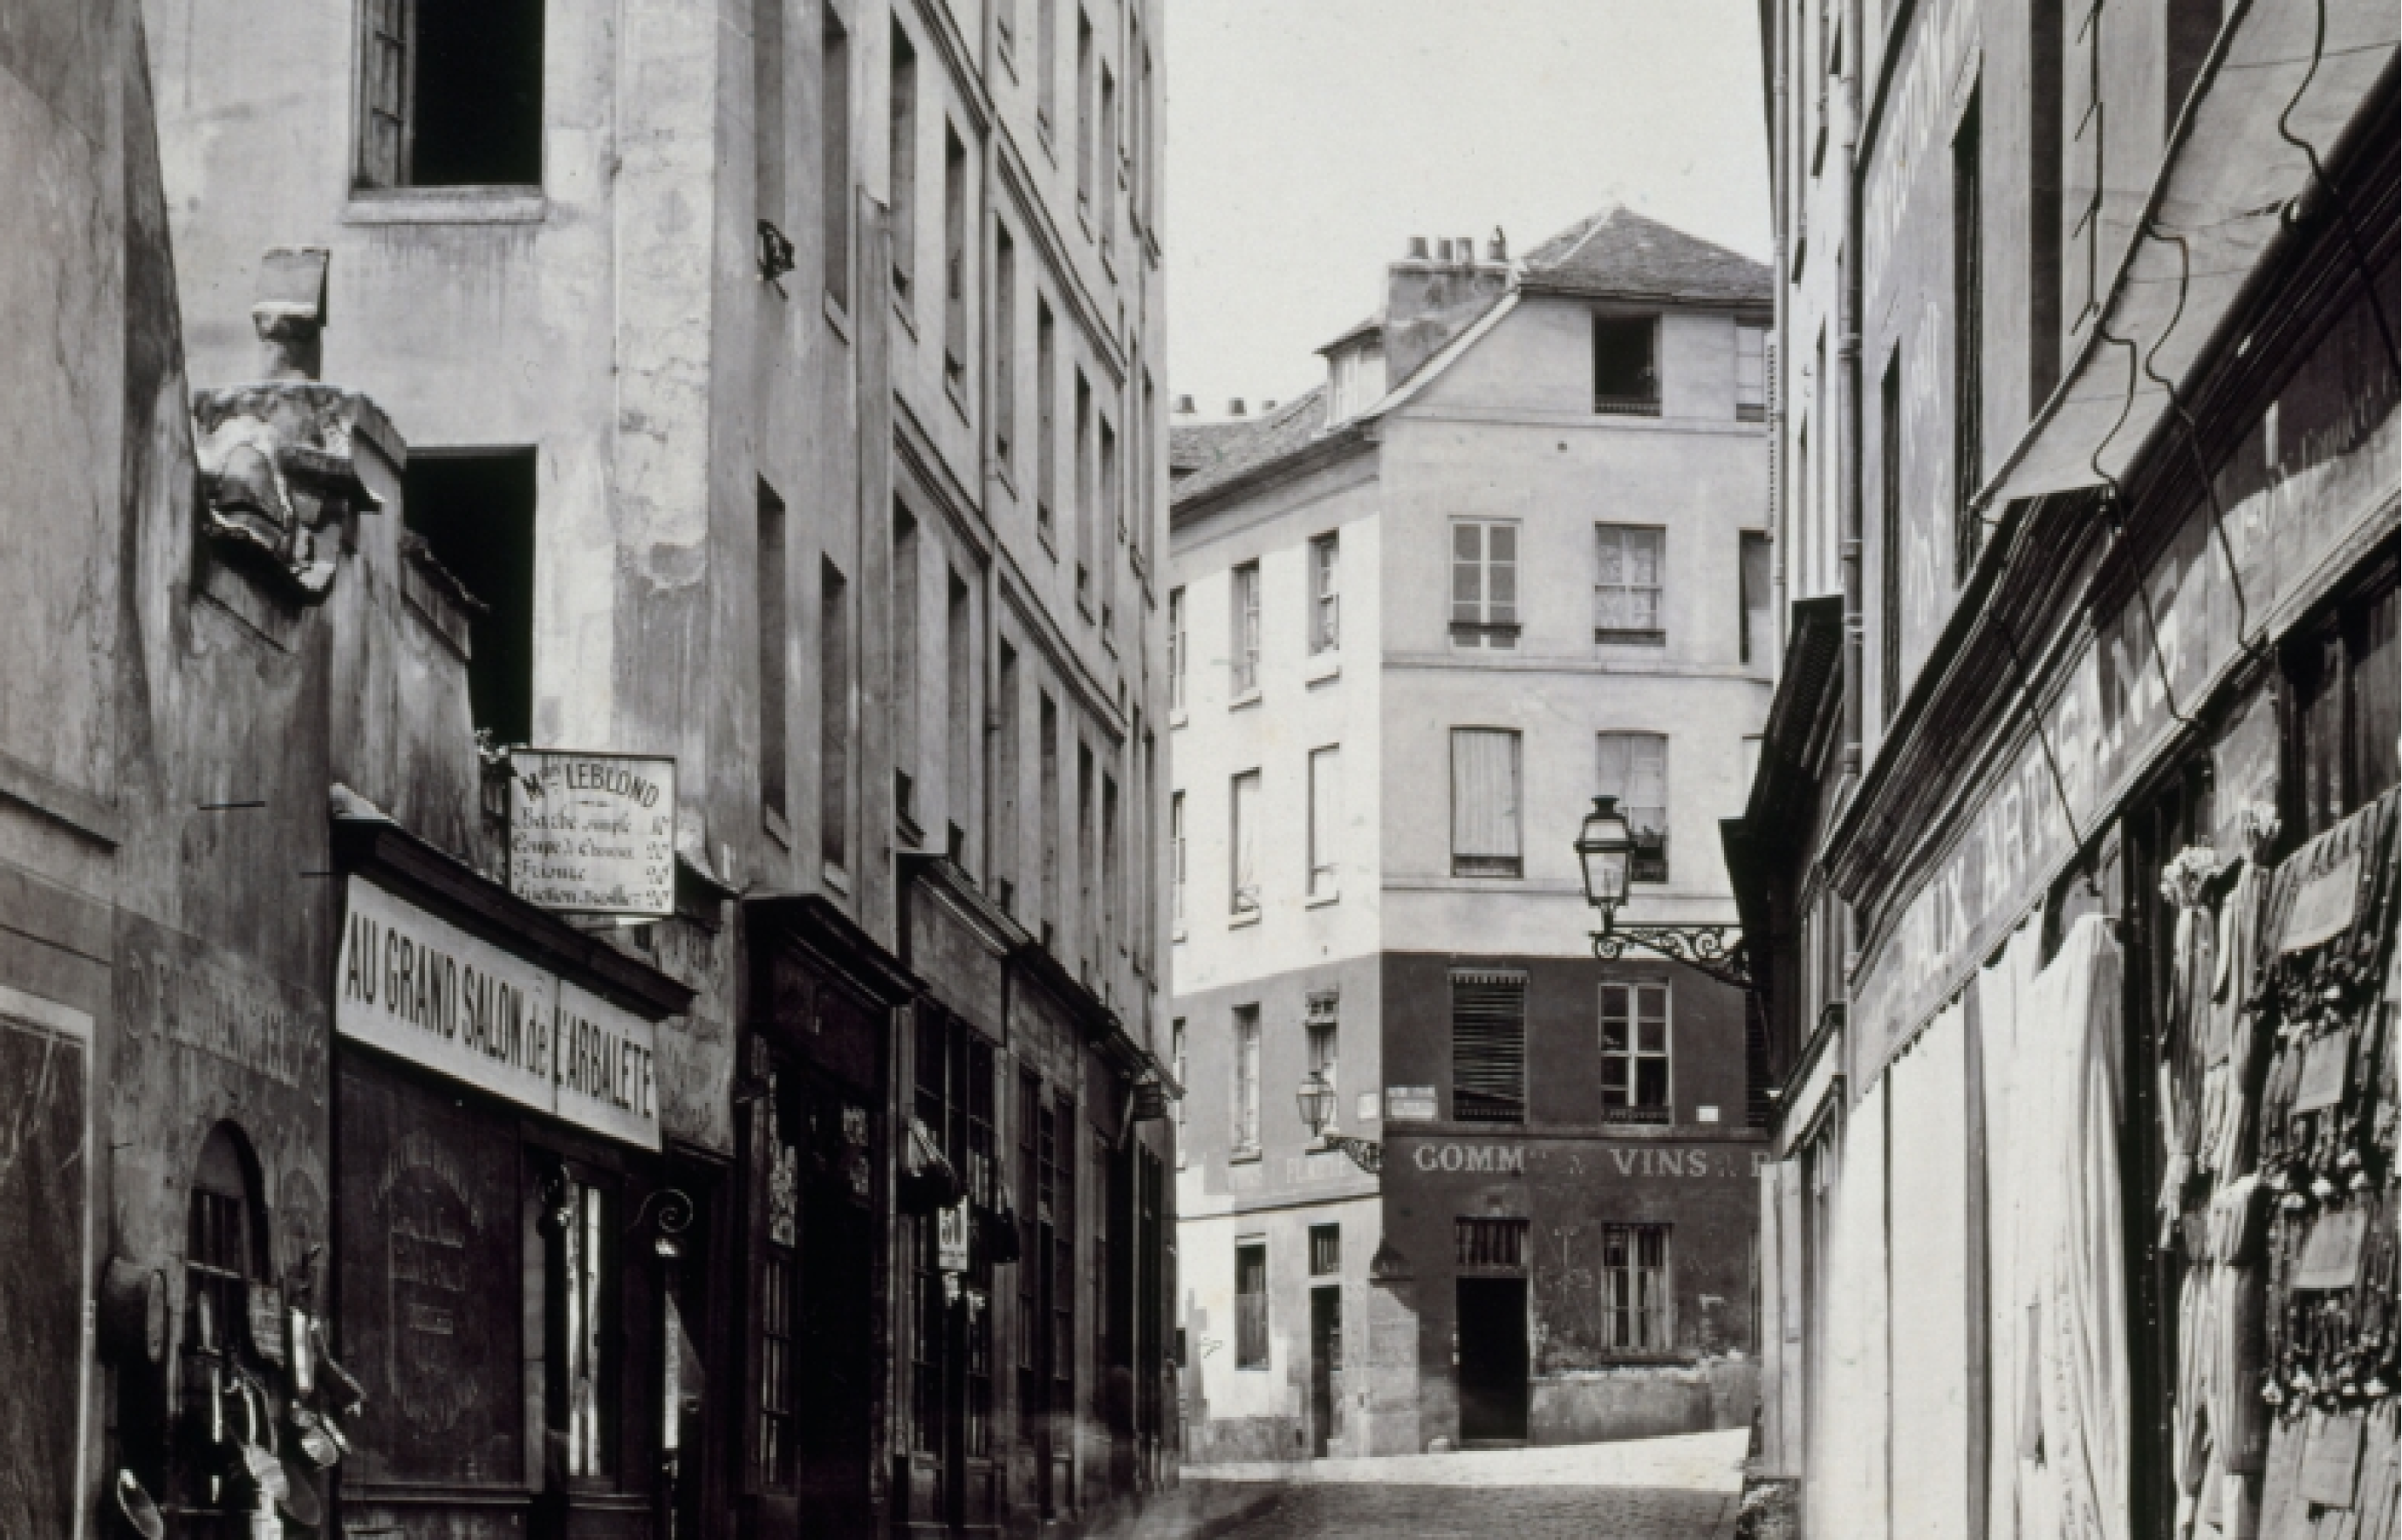
\includegraphics[width=\textwidth]{extrait_icono2.png}
                \caption{La rue de l'arbal�te, photographie de Charles Marville, entre 1865 et 1867}
                \label{fig:marville}
        \end{subfigure}%
         \caption{Sources iconographiques}
	\label{fig:icono}
\end{figure}

\myparagraph{Sources arch�ologiques}
Les sources arch�ologiques d�signent l'ensemble des artefacts des structures urbaines anciennes issus de travaux de fouille, permettant une restitution physique de la ville non plus au travers de documents dont les biais peuvent �tre difficilement identifiables, mais au travers de donn�es arch�ologiques restituant plus objectivement les b�timents anciens sur le parcellaire actuel.
Il s'agit aussi d'objets complexes, fragment�s, accumul�s au cours du temps, permettant surtout une �tude locale plut�t qu'un raisonnement � l'�chelle de la ville \citep{Galinie2000}.
Diff�rents travaux portent sur l'utilisation de tels artefacts pour reconstituer un espace pass�, parmi eux les travaux de \cite{Rodier2010}, \cite{DeRunz2008} ou \cite{Stefani2010}.


\myparagraph{Le terrain de la ville actuelle}
L'espace de la ville actuelle est le produit de la s�dimentation au cours du temps d'une multitude de tissus et de structures, il est un \emph{conservatoire temporel} \citep{Lepetit1996}.
La ville actuelle comporte alors les traces de tous ces espaces pass�s, directement accessibles lorsqu'il s'agit d'objets urbains ou d'�l�ments architecturaux ayant surv�cu � l'�preuve du temps,
ou bien indirectement � travers la persistance dans le tissu urbain de structures anciennes \citep{Ducom2009}.
La ville actuelle constitue pour l'historien une source d'informations � part enti�re, mais aussi un appui pour comprendre les structures urbaines d�crites dans des sources anciennes.


\subsection{Le plan de ville au c\oe ur de la repr�sentation visuelle d'un espace urbain ancien}
\label{subsection:plans}
\subsubsection{Le socle d'une repr�sentation de l'espace ancien}

\myparagraph{Processus de communication cartographique}
Nous avons abord� en d�but de section la notion de repr�sentation cartographique, dont nous avons pr�sent� succinctement l'adaptation � un travail historique qui se fonde sur les traces survivantes d'un �tat ancien de la ville.
Les sources cartographiques sont des traces particuli�res en ceci qu'elles sont des repr�sentations visuelles concr�tes et globales des anciennes structures, � la diff�rence par exemple d'un texte qui, aussi pr�cis qu'il soit dans sa description des lieux, fait appel � l'imagination du lecteur.

\subparagraph{}
Une carte ancienne est �galement un objet complexe.
En effet, elle est une trace et par cons�quent il existe une rupture temporelle entre le moment de sa cr�ation et le moment de sa lecture \citep{Kramer2012}.
Le cr�ateur et le lecteur de la carte sont diff�rents et appartiennent � des �poques �galement diff�rentes.
Qu'il s'agisse de construire une carte ou de la lire, les deux op�rations font appel � des processus cognitifs de perception de l'espace qui, par plusieurs phases de filtrages (des sens, culturels, etc.) d�forment la r�alit�.
Sans aller plus loin sur ces processus (pour lesquels on pourra se r�f�rer � \cite{Bailly1977, Bailly1985}), il faut prendre en consid�ration le double filtrage qui r�sulte~: de la repr�sentation cartographique d'un espace par un cartographe; de sa lecture plus tardive par une autre personne dans un contexte culturel et historique diff�rent.
\subparagraph{}
Ce processus de transmission d'un message et les d�formations qu'il subit lors de son codage au sein d'une carte puis son d�codage, sont abondamment abord�s dans le domaine de la cartographie \citep{Dodge2012}.
Afin de clarifier notre propos, nous proposons de nous appuyer sur un mod�le de communication cartographique propos� par \cite{Salitchev1978}, r�sum� dans le sch�ma \ref{fig:schem_salitchev}.
Dans ce mod�le, une part de la r�alit� est d'abord observ�e par le cartographe qui souhaite la cartographier (1).
Il effectue alors une s�lection des �l�ments qu'il souhaite repr�senter et r�unit les informations n�cessaires � leur description par divers moyens d'acquisition (observation visuelle, lev� topographique, etc.)(2).
L'information g�ographique alors constitu�e est encod�e et �ventuellement g�n�ralis�e au sein d'une carte au moyen de symboles cartographiques (3).
La carte, une fois construite, peut �tre d�cod�e (lue) par un individu qui poss�de une connaissances des symboles cartographiques utilis�s, lui permettant d'obtenir une somme d'informations g�ographiques.
Finalement, le lecteur interpr�te ces informations en fonction de son exp�rience et de l'�tat de ses connaissances sur la r�alit� repr�sent�e, agrandissant alors ses connaissances sur cette r�alit� (4).
Cependant, puisque les connaissances et l'exp�rience varient d'un lecteur � l'autre, la part de r�alit� ainsi enrichie varie �galement.
\begin{figure}[ht]
  \centering
  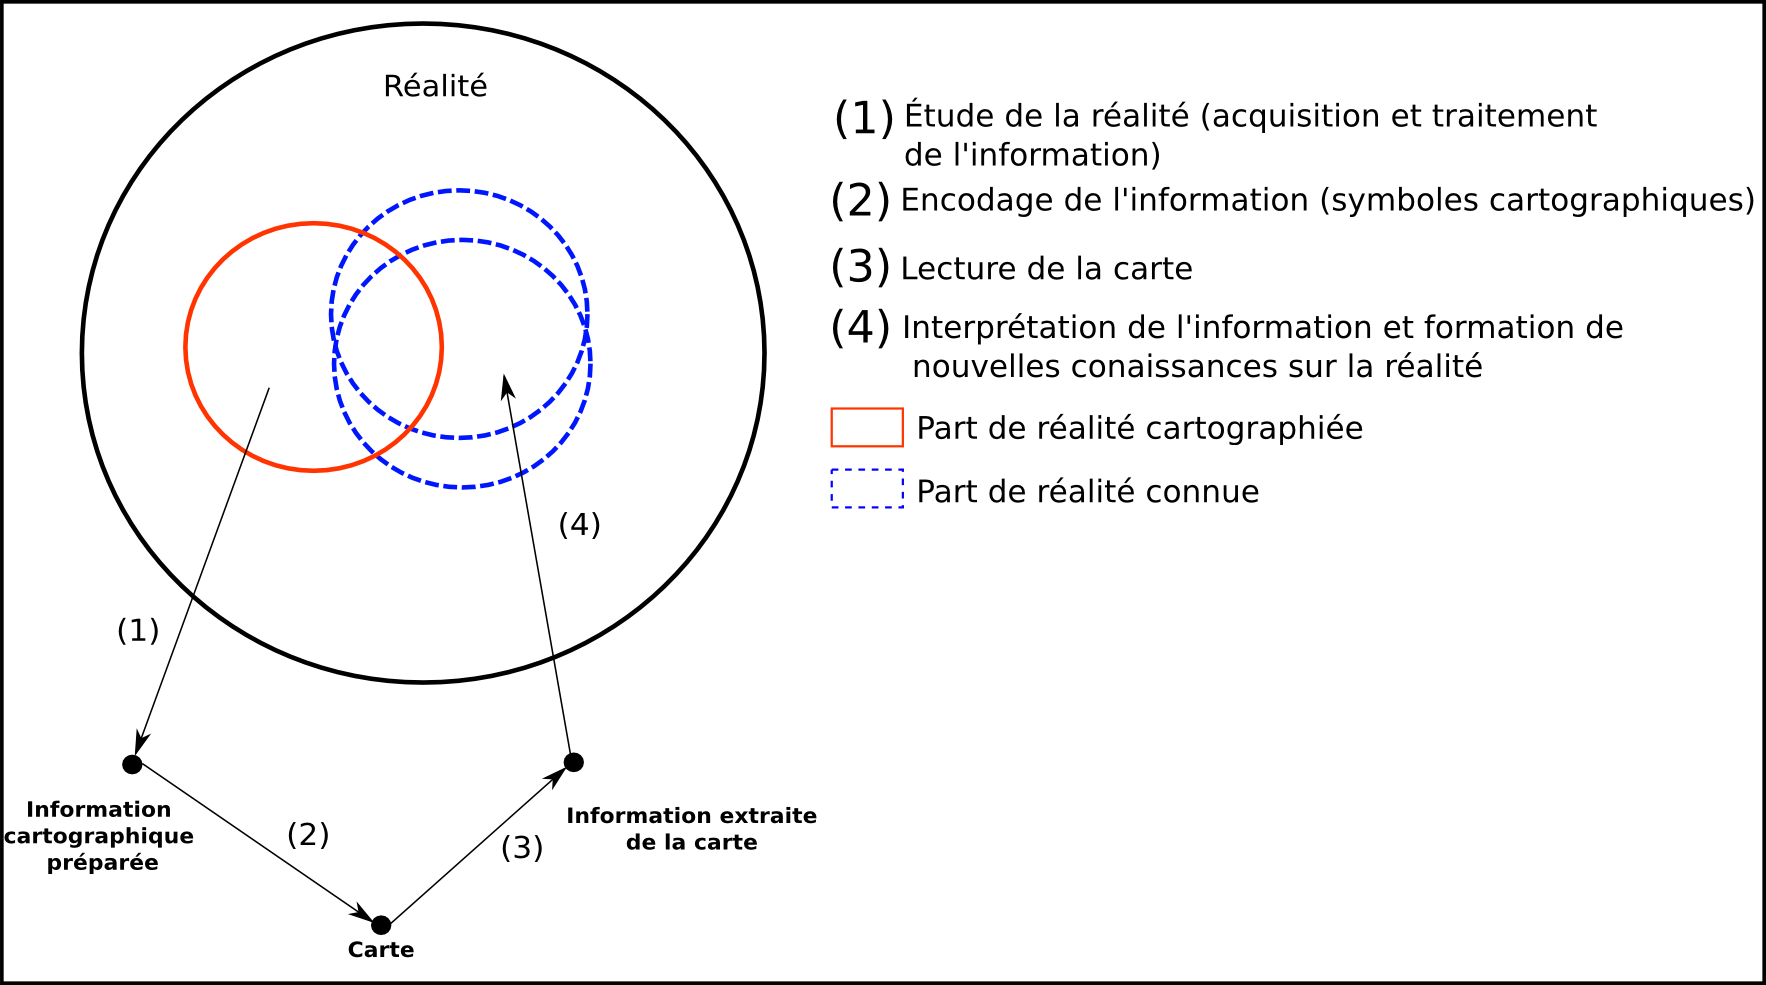
\includegraphics[width=1\textwidth]{comm_carto_salitchev.png}
\caption{Le processus de communication cartographique de \cite{Salitchev1978}}
  \label{fig:schem_salitchev}
\end{figure}

\myparagraph{Processus de communication cartographique diff�r�e}
\label{paragraph:comm_caro_differee}
Lorsqu'il s'agit de lire une carte ancienne, la rupture temporelle existant entre la production de la carte et sa lecture cr�e deux sp�cificit�s.
Nous proposons alors d'adapter le sch�ma de \cite{Salitchev1978} dans le cadre d'une lecture de carte ancienne en mod�lisant une communication diff�r�e.
Bien s�r, comme nous l'avons abord� pr�c�demment, toute communication cartographique g�n�re un d�calage entre le message transmis par le cartographe et sa r�ception par un lecteur.
Cependant dans le cas de cartes historiques le d�calage est tel que la r�alit� du cartographe et celle du lecteur sont sensiblement diff�rentes.
Cette rupture am�ne deux particularit�s~:
\begin{itemize}
 \item Le \textbf{temps �coul�} entre la production de la carte et sa lecture est tel que cette derni�re ne peut arriver qu'apr�s une phase de pr�servation de la carte.
Il peut s'agir simplement d'un archivage du document cartographique, mais aussi d'une survivance du message au travers de r�utilisations plus tardives.
\cite[p. 10]{Pinon2004} en fournit un exemple parlant~: 'original du premier plan de Paris dress� vers 1523-1530) a �t� perdu, mais il reste connu au travers de diverses copies.
 \item L'augmentation de la connaissance ne porte pas sur la r�alit� du lecteur, mais sur une \textbf{r�alit� ant�rieure} � laquelle il n'a pas acc�s.
D�s lors, il dispose d'une base de connaissances plus faible pour interpr�ter le message cartographique transmis.
Le risque est alors d'accorder un cr�dit trop grand, par manque d'informations, � une carte ancienne dont le degr� de r�alisme d�pend fortement des biais de repr�sentation (volontaires ou non) introduits par le cartographe.
\end{itemize}
Le sch�ma adapt� est pr�sent� par la figure \ref{fig:comm_carto_traces}.
La r�alit� n'est plus repr�sent�e comme fig�e dans le temps, mais le cylindre indique son �volution.
Le d�roulement de la communication cartographique se d�roule alors �galement dans le temps, la hauteur de chaque point et fl�che indiquant ce d�roulement.
L'�tape (3) d�crit la phase de pr�servation du document, tandis que la fl�che qui reviens dans le temps (5) illustre l'acquisition d'une connaissance non pas sur la r�alit� pr�sente du lecteur, mais sur celle pass�e du cartographe.
Finalement, le d�grad� en (1) illustre la phase d'acquisition de l'information g�ographique, qui elle aussi n'est plus instantan�e mais dure pendant un certain temps~: l'information encod�e est alors non plus un instantan� de la r�alit� mais une accumulation de temporalit�s diff�rentes.
Les portions de r�alit�s per�ues ou �largies ne s'�talent alors pas seulement dans l'espace, mais �galement dans le temps.

\begin{figure}[ht]
  \centering
  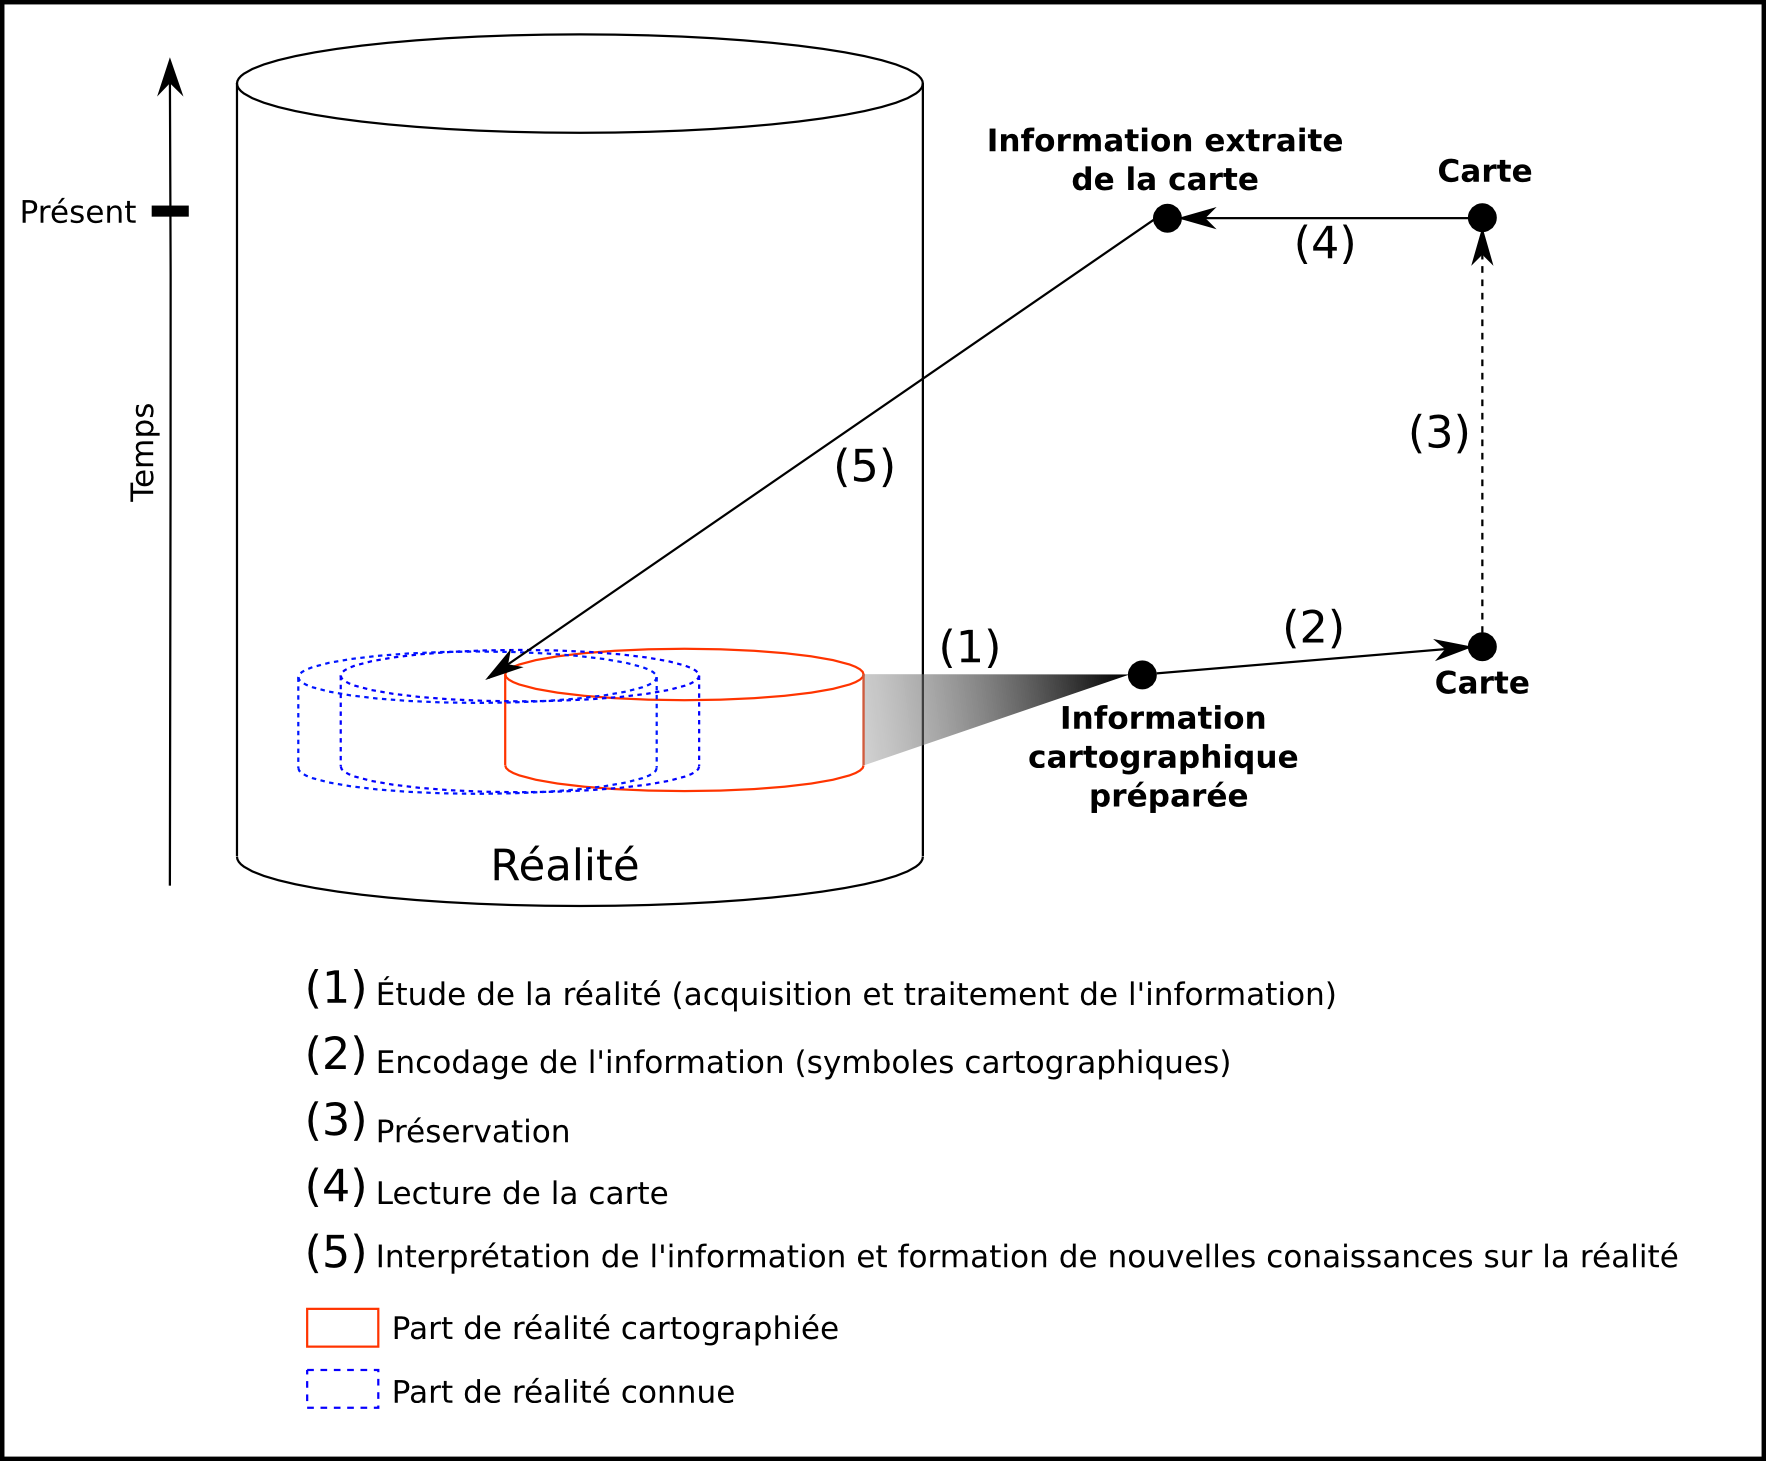
\includegraphics[width=1\textwidth]{comm_carto.png}
\caption{Le processus de communication cartographique de \cite{Salitchev1978} adapt� pour la lecture de traces historiques dans des cartes.}
  \label{fig:comm_carto_traces}
\end{figure}

% \myparagraph{Des atouts particuliers}
% Les sources cartographiques ont l'avantage de permettent d'englober d'un coup tout un espace. En plus, la repr�sentation visuelle est bien plus efficace pour une compr�hension rapide de la disposition des �l�ments de l'espace. En plus de cela, les cartes ne comportent rarement que des indications topographiques. Elles portent souvent de nombreux toponymes qui peuvent donner des indices historiques. Bien sur ce sont souvent les noms de rue. Ca peut �tre les noms des �difices, ou les adresse. La l�gende elle m�me indique beaucoup : trac�s projet�s, status de la voie, travaux.  
% 
% \myparagraph{Lire les transformations de l'espace dans les plans}
% Le plan est une tranche d'un moment dans la ligne du temps. De ce fait, il ne donne � priori pas � lire les transformations de l'espace. Pourtant il n'est pas muet. Une technique tr�s utilis�e consiste simplement � mettre c�te � c�te ou � superposer plusieurs plans anciens de fa�on � lire les transformations dans les changements observ�s entre 2 couches.
% 
  
\subsubsection{Types de plans}
Les sources anciennes sont des \emph{miroirs d�formants du pass�} \citep{Spitzer1999}.
Ces d�formations r�sultent de divers causes que nous aborderons en d�tails dans la section \ref{section:imperfections}.
Cependant, les effets du temps dans la conservation du message cartographique ou dans sa construction m�me sont des facteurs de d�formations important.
Outre le temps, la multitude d'objectifs d�finis par les commanditaires des plans ou les cartographes eux-m�me peuvent impacter fortement le la pr�cision d'une repr�sentation cartographique.
Afin d'identifier les principales diff�rences entre plans de villes et par l� les causes de d�formations du pass�, nous nous appuyons sur une s�paration en deux classe bas�e sur les objectifs des plans, propos�e par \cite{Pinon2004}.

\myparagraph{Plans fonciers}
Les plans fonciers d�signent l'ensemble des plans, sur l'ensemble de la ville ou un espace restreint, dont l'objectif est de d�crire la r�partition spatiale des propri�t�s fonci�res, c'est � dire le tissu parcellaire de la ville.
\`A Paris, les plans parcellaires apparaissent � partir du XVII\up{e} si�cle, permettant une repr�sentation plus claire des limites de propri�t�s jusqu'alors mat�rialis�es par des rep�res divers telles des bornes.
\cite{Arnaud2008} distingue les plans parcellaires selon trois contextes d'utilisation~: juridique, fiscal et administratif.
\subparagraph{}
Dans le contexte juridique, les plans parcellaires visent � aider la r�solution de conflits entre deux parties revendiquant, par exemple, des droits sur un m�me emplacement \footnote{C'est par exemple le cas du plan de Quesnel � Paris}.
Les plans parcellaires fiscaux servent quant � eux d'outil pour la r�partition et le calcul d'un imp�t.
Ainsi dans le Paris de l'ancien r�gime apparaissent � partir du XVII\up{e} si�cle les plans des censives, dress�s par diff�rentes seigneurs fonciers la�cs ou eccl�siastiques ayant droit de perception du cens sur leurs possessions parisiennes \footnote{Pour plus d'informations sur les censives parisiennes, voir les travaux de \cite{Weiss2009}}.
\subparagraph{}
On retrouve �galement dans cette cat�gorie le Papier-terrier du Roi, ex�cut� de 1700 � 1726-1727, d�crivant pour Paris et ses faubourgs chacune des parcelles quelque soit le propri�taire foncier la poss�dant associ� � un plan d�taill� de chaque zone.
Enfin, il s'agit aussi de plans administratifs pr�cis, servant alors de base � des travaux cartographiques.
Si son but est �galement fiscal, rentre dans cette cat�gorie le cadastre napol�onien dont la justesse g�om�trique et l'�chelle (1/2000 sur Paris) en fait une base pour la construction de plans de la ville.

\myparagraph{Plans topographiques et projets}
Les plans topographiques sont des outils d'am�nagement de la ville, destin�s � faciliter la compr�hension et la mise en place d'interventions urbaines.
Ils sont une repr�sentation �pur�e de la ville, l'accent �tant plac� sur la justesse g�om�trique et la fid�lit� � la morphologie des �l�ments urbains.
Les plans projets visent la m�me pr�cision g�om�trique, mais leur but diff�re.
Ces plans sont directement li�s � un projet urbain, pr�parant, pr�sentant ou faisant le bilan du projet.
\subparagraph{}
Si la distinction est faite entre plans topographiques et plans projets, il n'est pas �vident de distinguer les deux, les plans pouvant m�ler diff�rents messages pour livrer une vision d'un espace urbain certes pr�cise, mais modifi�e par des projets li�s aux commanditaires du plan \citep{Pinon2004}.
Par exemple, le plan de Verniquet vise et atteint une grande pr�cision g�om�trique en fournissant une description riche et compl�te de Paris.
Mais il aussi porte le trac� de diff�rents projets de percements de voies qui ne seront pas toujours r�alis�s.

\subsubsection{Complexit�s temporelles des plans anciens}
\myparagraph{Le temps du plan}
\label{paragraph:map_is_not_instant}
� la diff�rence d'autres repr�sentations visuelles comme la photographie, la carte ne repr�sente pas la configuration de l'espace � un moment donn�, bien qu'elle en offre une repr�sentation statique.
En effet, la carte prend n�cessairement un temps variable pour �tre construite, pendant lequel l'espace qu'elle repr�sente continue � se transformer.
Si cet aspect peut �ventuellement �tre n�glig� lorsqu'il s'agit de cartes r�centes, la dur�e de lev� des plans anciens, s'�talant souvent sur plusieurs ann�es, oblige � prendre en compte cette temporalit� interne au plan.
La source cartographique ancienne doit alors �tre consid�r�e comme un empilement de fragments de l'espace repr�sent� � des moments diff�rents.
� un plan ne correspond donc pas un instant, mais plut�t une p�riode pendant laquelle le plan est consid�r� comme une repr�sentation fiable de l'espace.
\subparagraph{}
Cette p�riode ne peut �tre d�finie qu'au cas par cas, mais nous consid�rons par d�faut qu'il s'agit de la p�riode pendant laquelle le plan est lev�, correspondant au moment o� les mesures trigonom�triques sont effectu�es sur le terrain, et donc o� le d�calage temporel entre le plan et l'espace r�el est moindre.
Qu'elle corresponde au lev� du plan ou soit d�finie par un exemple, cette dur� correspond au \emph{temps valide} des bases de donn�es temporelles \citep[p. 189]{NGuyen2006}~: \emph{un instant pr�cis auquel se produit un �v�nement, [ou] un intervalle de temps qui d�finit la dur�e de validit� des valeurs des donn�es associ�es}.
Nous nommons donc cette p�riode \textbf{temps valide du plan}.


\myparagraph{Types de plans par �poque}
 Au del� de cette sp�cificit�, \cite{Pinon2004} distinguent deux cat�gories de plans anciens selon leurs modes de cr�ation mais �galement selon leurs �poques~:
\begin{itemize}
 \item \textbf{Plans th�matiques}~: Il s'agit de plans command�s par un individu ou une institution, et confi�s � un cartographe.
R�pondant aux demandes des commanditaires, ces plans sont orient�s vers une repr�sentation mettant en valeur un �l�ment particulier de la ville ou la cit� dans son ensemble, sans forc�ment de consid�ration profonde pour la justesse g�om�trique des trac�s.
� Paris, les plans de Gomboust, De La Caille et Bullet en constituent des exemples pour les XVII\up{e} et XVIII\up{e} si�cles, ceux de Vasserot et Bellanger ou de Alphand pour le XIX\up{e} si�cle.
 \item \textbf{Plans topographiques}~: Il s'agit souvent de plans dont les lev�s sont pr�vus par le cartographe lui-m�me, lequel cherche ensuite un client pr�t � financer la production de la carte.
Ces plans visent � plus d'exactitude g�om�trique et repr�sentent la ville de fa�on plus neutre, s'attachant d'avantage aux structures m�me de l'espace qu'� d'�ventuels enjeux politiques.
Dans cette cat�gorie rentrent notamment des plans tels que ceux de Delagrive, Verniquet ou encore Delisle, tous int�gralement ou en partie financ�s sur fonds propres du cartographe.
\end{itemize}
\subparagraph{}
Bien sur, les fronti�res entre ces deux cat�gories ne sont pas �tanches.
Par exemple, le plan de Jacoubet \citep{MAPJacoubet} est une commande du pr�fet de la Seine visant la pr�cision g�om�trique et une description relativement �pur�e de la ville.
De plus, cette classification se base sur une distinction entre commanditaires ''officiels'' et initiatives priv�s.
Cependant, les commanditaires de nombreux plans sont inconnus, tels que ceux de Benedict Vassalieu \citep{MAPVassalieu} et Albert Jouvain de Rochefort \citep{MAPRochefort} sur Paris.
D'apr�s \cite{Pinon2004}, les d�dicaces indiqu�es dans ces plans ne constituent en rien une d�signation suffisante d'un �ventuel commanditaire.
Enfin, certains plans sont � mi-chemin des deux cat�gories, comme le plan de Verniquet \citep{MAPVerniquet}, commenc� par une initiative priv�e puis financ� par les pouvoirs officiels.
Malgr� la porosit� de cette fronti�re, la consid�ration de ces diff�rents �l�ments nous permet de pr�ciser les complexit�s engendr�es par la temporalit� propre aux plans.

\myparagraph{Multiplicit� temporelle}
Qu'il s'agisse de plans th�matiques ou purement topographiques, il peut coexister au sein d'un plan des repr�sentations issues de p�riodes diff�rentes pr�sent�es sur un m�me fond de carte.
La figure \ref{fig:multitemp} illustre un tel cas sur diff�rents plans th�matiques pr�sentant les interventions urbaines effectu�es dans Paris au XIX\up{e} si�cle.
Dans le cas de la carte topographique, bien que l'objectif soit de repr�senter la ville au moment du lev�, le plan comporte �galement des trac�s de rue en projet, dont le percement n'est pas commenc� et qui n'ont donc aucune r�alit� physique au moment du lev� du plan.
Pour la carte th�matique, il s'agit cette fois de repr�senter un historique et des �v�nements ant�rieurs sur un plan de Paris, r�sultant ici aussi en une accumulation de temporalit�s au sein de la source.

\begin{figure}[ht]
	\centering
		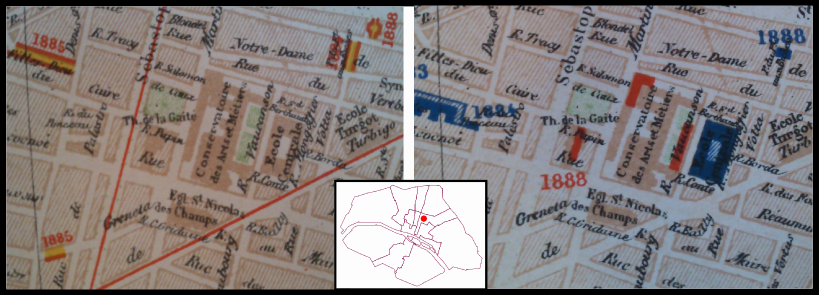
\includegraphics[width=0.8\textwidth]{multitemp.png}
	\caption{Diff�rentes temporalit�s au sein d'une m�me carte~: les travaux de voirie effectu�s et �difices construits de 1789 � 1889, d'apr�s \cite{Huet1889} }
	\label{fig:multitemp}
\end{figure} 
\myparagraph{Dur�e des op�rations de lev�s}
Comme nous l'avons introduit, le trac� d'un plan de ville complet n'est pas une op�ration rapide et n�cessite une ou plusieurs campagnes de lev�s, �talant la p�riode de construction du plan sur plusieurs ann�es alors que l'espace urbain continue de se transformer.
Lors de la production finale du plan, celui-ci contient alors des informations provenant de phases d'observation de la ville � des moments diff�rents, pouvant mener � des anachronismes.
Par exemple, le plan de Verniquet \citep{MAPVerniquet} fit d'abord l'objet d'un lev� � partir de 1775, suivi par un second entre 1785 et 1795.
%\begin{figure}[ht]
%	\centering
%		
\includegraphics[width=0.01\textwidth]{void.png}
%	\caption{\'Etalement des lev�s du plan de Verniquet et minutes}
%	\label{fig:minutes_verniquet}
%\end{figure} 

\myparagraph{R�utilisation de plans}
Lever un plan �tant une op�ration longue et co�teuse, la construction d'un plan est parfois effectu�e sur la base d'un plan plus ancien.
Sur Paris par exemple, de nombreux plans du XIX\up{e} si�cle r�utilisent le plan de Verniquet trac� au moment de la R�volution fran�aise, ce qui est notamment le cas de plans tr�s largement utilis�s par l'administration de l'�poque, comme l'Atlas de Jacoubet \citep{MAPJacoubet} ou plan de Girard \citep{MAPGirard}.
Cette r�utilisation peut avoir comme cons�quence un effet d'anachronisme qui se produit entre la p�riode de publication du plan et l'espace qu'il repr�sente r�ellement. Cette pratique induit aussi la reproduction des �ventuelles erreurs pr�sentes dans les op�rations de lever et de gravure du premier plan.
\begin{figure}[ht]
	\centering
		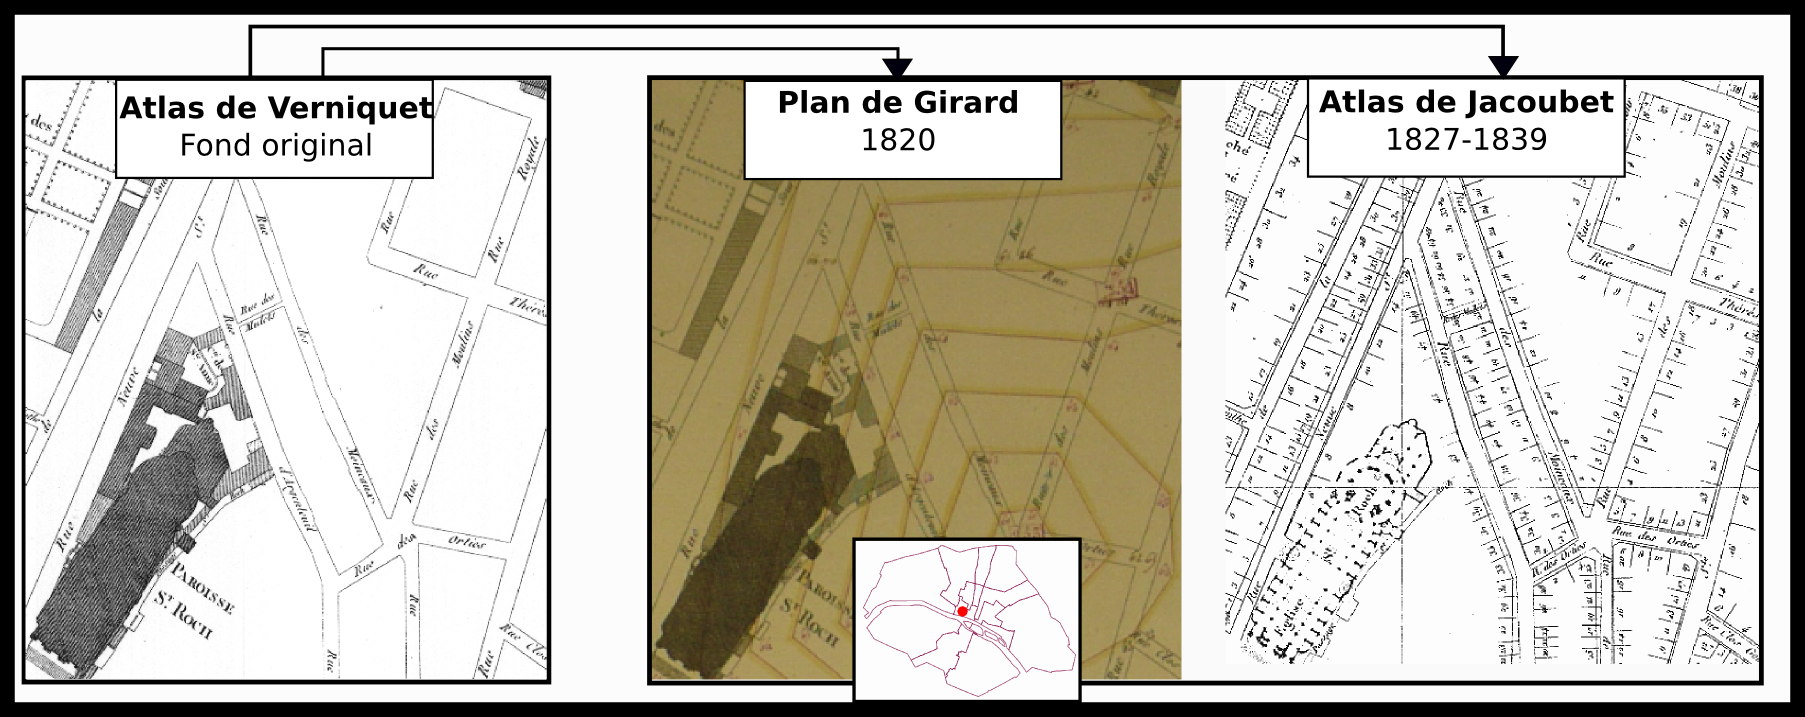
\includegraphics[width=0.8\textwidth]{reuse.png}
	\caption{R�utilisation du plan de Verniquet (� gauche) dans deux plans plus tardifs (� droite)}
	\label{fig:base_verniquet}
\end{figure} 

%
%\begin{center}
%\fcolorbox{black}{white}{
%  \begin{minipage}[t]{0.9\textwidth}
%\begin{center}
% \textbf{R�sum� de la section}
%\end{center}
%La cartographique permet de reconstruire, � partir de sources diverses, une repr�sentation globale d'un espace ancien qui peut alors devenir le support � la spatialisation de donn�es sociales, ou bien un outil d'analyse des formes de la ville et de leurs transformations.
%La reconstitution d'un espace urbain peut se r�v�ler un processus d�licat, les sources g�ohistoriques �tant h�t�rog�nes dans leurs formes et leurs contenus.
%\subparagraph{}
%Dans cette section, nous avons sugg�r� une typologie des sources g�ohistoriques permettant de reconstituer les transformations morphologiques d'un espace donn�. Nous avons aussi montr� que chaque type de source comporte des sp�cificit�s et certains biais. En particulier, lorsqu'il s'agit de repr�senter les structures d'un espace ancien, il existe une diff�renciation importante entre les sources fournissant des donn�es spatiales dont les formes et la localisation sont explicitement repr�sent�e (les cartes, les �l�ments architecturaux, les artefacts arch�ologiques et les iconographies) et les sources textuelles dont les informations spatiales doivent �tre localis�es .
%\subparagraph{}
%Les cartes anciennes constituent la source principale de repr�sentation de l'espace ancien.
%Les plans de villes donnent des vues souvent globales en fournissant de nombreuses informations~: les structures spatiales d'abord, mais �galement des informations s�mantiques (toponymes, structure des b�tis, etc.).
%Ces plans sont cependant des sources complexes et h�t�rog�nes, dont il est important de conna�tre les particularit�s en vue de l'extraction des informations qu'ils contiennent et de son utilisation dans un SIG.
%Nous avons identifi� les causes de cette h�t�rog�n�it� qui marque la nature de ces sources. alors les diff�rentes causes de cette h�t�rog�n�it�, et pointons les complexit�s internes de ces plans.
%Le temps de construction des plans, avant tout, mais aussi les biais induits par les finalit�s des cartographes et commanditaires apparaissent en particulier comme autant de points critiques qui demandent � �tre analys�s avant l'utilisation d'un plan.
%\end{minipage}
%} 
%\end{center}


\section{L'apport des  SIG pour �tudier l'histoire~: un choix m�thodologique}
\label{section:SIG}
\subsection{Introduction~: d�finitions pr�alables}
\myparagraph{Des Syst�mes d'Informations G�ographiques...}
Il n'existe pas une d�finition unique des Syst�mes d'Informations G�ographiques (SIG), mais diff�rentes approches issues des diverses disciplines qui se sont int�ress�es aux donn�es g�ographiques \citep{Denegre1996}.\footnote{Notons d�s � pr�sent que dans les travaux pr�sent�s au sein de cette th�se, l'acronyme anglais ''GIS'' correspond syst�matiquement �  \emph{Geographic Information System}.
Lorsqu'un homonyme est utilis� (comme \emph{Geographic Information Science}), l'acronyme ne sera pas utilis� pour �viter les confusions.}.
La relative jeunesse de la g�omatique ainsi que le fort attrait pour la repr�sentation d'une information spatiale ou spatialis�e au sein de divers domaines (scientifiques, industriels, �ducatifs, etc.) ont engendr� une multiplicit� d'usages, d'applications rassembl�s sous le m�me sigle \citep{Chrisman1999}.
\subparagraph{}
On peut avoir une appr�ciation indirecte de la vari�t� de dimensions qui marque l'horizon de ce domaine en �voquant~\citep{Denegre1996} deux d�finitions qui synth�tisent les principales approches existantes~: d'une part, une vision technique des SIG issue principalement de l'informatique, d'autre part un point de vue centr� sur l'utilisation de ces syst�mes pour r�pondre � des besoins th�matiques.
\begin{itemize}
 \item La premi�re d�finition est elle m�me une synth�se de diverses propositions issues de la g�omatique, de l'informatique ou de la g�ographie, et qui peut �tre r�sum�e par la d�finition adopt�e par la Soci�t� Fran�aise de T�l�d�tection \footnote{http://www.sfpt.fr/}~: \emph{ un syst�me informatique permettant, � partir de diverses sources, de rassembler et d'organiser, de g�rer,d'analyser et de combiner, d'�laborer et de pr�senter des informations localis�es g�ographiquement, contribuant notamment � la gestion de l'espace}.
Dans cette optique, on consid�re �galement des syst�mes d'informations au sens plus g�n�ral du terme et pouvant �tre constitu�s de proc�dures manuelles.
Les outils logiciels, les processus de traitement de l'information spatiale, mais �galement les bases de donn�es g�ographiques entrent dans cette cat�gorie.
\item La seconde d�finition est plus proche de l'usage fait de l'information g�ographique dans des domaines autres que la g�omatique et se focalise d'avantage sur les donn�es et leur exploitation.
Un SIG est ainsi d�fini comme \emph{un ensemble de donn�es rep�r�es dans l'espace, structur� de fa�on � pouvoir en extraire commod�ment des synth�ses utiles � la d�cision}~\citep{Didier1990}.
Il ne s'agit plus de s'int�resser aux syst�mes de traitement de l'information g�ographique eux m�mes, mais aux donn�es structur�es qui en sont issues et qui constituent la base d'un travail th�matique (production de cartes, analyse spatiale, etc.).
\end{itemize}
Ces deux d�finitions sont particuli�rement int�ressantes dans la mesure o� elles montrent finalement deux visions diff�rentes des syst�mes d'informations g�ographiques, l'une provenant des domaines � l'origine des syst�mes eux m�me, la seconde correspondant � la vision des utilisateurs finaux de ces outils.
Pourtant, elles sont aussi compl�mentaires, chacune se positionnant � des endroits diff�rents du m�me syst�me de manipulation d'informations g�ographiques.
Si cette multiplicit� peut sembler uniquement formelle, elle est en fait source d'une ambigu�t� importante dans la d�signation des SIG destin�s � des travaux historiques.

\myparagraph{... aux Syst�mes d'Informations G�ographiques Historiques}
Les premi�res utilisations des SIG en histoire au d�but des ann�es 1990 ont donn� lieu � une explosion du nombre de travaux. C'est pourquoi on peut plut�t parler d'un ensemble d'�l�ments rassembl�s sous une d�nomination polys�mique que d'un �l�ment unique.
C'est pourquoi il nous para�t important de clarifier cette d�finition pour pouvoir nous positionner efficacement par rapport aux propositions existantes.
Le plus simple est sans doute d'�claircir cette notion � partir des �nonc�s que l'on retrouve dans la litt�rature. � ce niveau \citep{Knowles2008}, les SIG historiques peuvent d�signer en m�me temps~:
\begin{itemize}
 \item Les outils logiciels qui permettent de visualiser, stocker et analyser une information g�ohistorique issue de sources multiples.
 \item Les m�thodologies d'int�gration d'une information g�ohistorique au sein d'un outil SIG (logiciel ou base de donn�es).
\end{itemize}
Mises en rapport avec les d�finitions pr�c�dentes des SIG, il appara�t clairement que ces deux propositions s'ins�rent en plein dans la premi�re vision, que nous venons d'�voquer et qui exprime une approche principalement technique des SIG, car il s'agit ici de consid�rer des syst�mes sp�cifiquement d�di�s � l'analyse et au traitement de donn�es historiques.
Pourtant, on le voit, on parle aussi de SIG historique pour d�signer un ensemble de donn�es qui changent dans le temps~\citep{ALPAGE}. Dans cette optique, nous rejoignons donc davantage la seconde vision, ax�e non plus sur les outils informatiques eux-m�me mais sur les donn�es spatiales produites � partir de la collecte de sources d'archive ou d'observations arch�ologiques.
\subparagraph{}
Dans leurs travaux, \cite{Gregory2007} sortent des cat�gories d�j� identifi�es en parlant cette fois non plus des outils, des m�thodes ou des donn�es, mais de la discipline m�me �mergeant de l'utilisation des outils SIG dans le cadre d'�tudes historiques.
Cette proposition particuli�re est fondamentale car elle met en lumi�re la position des historiens comme utilisateurs principaux.
En effet, il s'agit plus souvent d'utiliser des outils existant et d'adapter leur usage � un probl�me historique que de mettre en place des outils SIG sp�cifiques.
Nous le constaterons plus pr�cis�ment en explorant les propositions d'outils existants dans la partie \ref{subsection:currgis}.
Les trois d�finitions pr�sent�es ici ne sont qu'un bref aper�u des �crits sur les SIG historiques, mais elles permettent de mettre en lumi�re deux besoins particuliers~:
\begin{itemize}
 \item \colorbox{red}{\textbf{H}} \textbf{G�rer des sources et des donn�es h�t�rog�nes}\\
Nous avons vu dans la section \ref{subsection:sources} que les sources historiques sont de nature, de forme, de contenu vari�s, induisant une forte h�t�rog�n�it� des donn�es qui peuvent en �tre extraites.
Nous avons vu dans la section \ref{subsection:sources} que les sources historiques, par la vari�t� de leu forme et leu contenu, induit une forte h�t�rog�n�it� des donn�es qui peuvent en �tre extraites. Par cons�quent, puisque la nature m�me du travail historique implique de croiser un nombre important d'informations diff�rentes, les SIG peuvent se r�v�ler des outils extr�mement efficaces utilisant la localisation spatiale comme pivot pour int�grer diff�rentes sources de donn�es.
Partant du constat que les sources historiques sont imparfaites et dont la fiabilit� n'est jamais totale, \cite{Knowles2008} avance �galement le besoin d'�tre capable de questionner toute donn�e sur l'origine et le degr� de fiabilit� de la source dont elle provient.
\item \colorbox{magenta}{\textbf{ST}} \textbf{Mod�liser et repr�senter les changements de l'espace dans le temps} \\
Comme le font remarquer plusieurs auteurs  \citep{Berman2009, Parker2010}, il s'agit de traiter et analyser des \emph{donn�es qui changent dans le temps}, c'est � dire des \textbf{donn�es spatio-temporelles}.
On retrouve ici l'importance de traiter non pas d'espaces fig�s, mais de ses transformations au cours du temps, qui doivent donc �tre g�r�es par un SIG sp�cifiquement dessin� pour les traitements historiques.
\end{itemize}
Il appara�t donc que ces deux �l�ments constituent des besoins essentiels auxquels un SIG d�di� � l'�tude de ph�nom�nes historiques doit pouvoir r�pondre.
S'il s'agit de besoins g�n�raux, ils sont pourtant fondamentaux et ils questionnent particuli�rement les syst�me existants.
En effet, l'absence d'h�g�monie d'un SIG particulier nous emm�ne � questionner l'ad�quation des outils et des m�thodes mis en place jusqu'� maintenant pour r�pondre � ces besoins.
Certains travaux, comme l'�tude du quartier des Halles effectu�e par \cite{Boudon1977} montrent d'ailleurs que les outils informatiques ne sont pas strictement n�cessaires pour travailler de mani�re cons�quente sur la morphologie d'un espace ancien et ses dynamiques de transformations.
Il nous faut donc explorer les raisons qui feraient des SIG des outils importants en histoire, et quels sont les objectifs pr�cis auxquels ils peuvent r�pondre.
Pour ce faire, nous proposons d'abord d'identifier les particularit�s du traitement de l'information g�ohistorique au sein d'un SIG, notamment quant � la manipulation de donn�es h�t�rog�nes et imparfaites (section \ref{section:imperfections}), puis d'expliciter ces objectifs et leur ad�quation avec le travail historique en section \ref{section:SIG}.
De l�, nous pourrons d�gager un positionnement plus clair pour notre travail.
% 
% 
% \subsection{Objectifs des SIG historiques}
% \subparagraph{}
% Nous avons jusqu'ici fait appara�tre les demandes que les historiens adressent aux SIG en tant qu'outils ou donn�es structur�es et localis�es. Les SIG ont �t� identifi�s par les historiens \citep{Gregory2007} comme pouvant apporter une meilleure compr�hension de ph�nom�nes historiques gr�ce � leur localisation dans l'espace et la mise en relation de donn�es spatialis�es. Cet objectif tr�s g�n�ral se trouve atteint par diff�rents moyens, que nous exposons tout en les mettant en relation avec les besoins identifi�s pr�c�demment et indiqu�s par leur couleur. Ainsi, l'objectif est de sp�cifier ces besoins en fonction des diff�rents buts des historiens et de mettre en place une classification des �l�ments qu'un SIG historique complet doit pr�senter pour s'adapter aux besoins d'un historien. Nous utiliserons par la suite cette classification pour analyser les SIG historiques existants.
% 
% \subparagraph{}
% Pour \cite{Gregory2007}, les SIG constituent un atout important pour l'enseignement de l'histoire.  Gregory et Healey identifient plus tard 3 objectifs sp�cifiques. On peut synth�tiser ces deux propositions autour des 3 points suivants : 
% Former des corpus de donn�es localis�es dans l'espace g�ographique
% Analyser les changements des structures spatiales au cours du temps, retracer les mouvements d'individus dans l'espace : analyse spatiale
% Fournir un moyen de visualisation de multiples donn�es et de confrontation des donn�es ainsi que de produciton de cartes.
% 
% 
% \myparagraph{Agr�gation et diffusion de donn�e spatiales et spatialis�es}
% Un des principaux buts recherch�s dans l'utilisation d'outils SIG en histoire est de pouvoir rassembl�s, dans un m�me r�f�rentiel spatial, un ensemble de donn�es et de sources historiques diverses dans un but p�dagogique (partage de ressources avec des �tudiants), pour des travaux collaboratifs ou plus simplement pour diffuser des donn�es, des r�sultats. La localisation dans l'espace est le r�f�rentiel qui permet de lier des donn�es h�t�rog�nes.
% Plus encore, il s'agit de placer dans l'espace des informations sociales diverses afin de les mettre en relation. EN PARLER MIEUX!
%  Ici, l'objectif du SIG est d'avantage de structurer et stocker l'information g�ohistorique plut�t que de fournir des outils d'analyse.
% 
% 
% \begin{itemize}
%  \item \colorbox{red}{\textbf{H}}-\smallskip-\smallskip-
% \end{itemize}
% 
% \myparagraph{Visualiser et produire des cartes}
% Le second objectif ressort d'un besoin de visualisation des donn�es sous forme de cartes. Il peut s'agir bien sur simplement de repr�senter les donn�es spatiales ou sociales localis�es, mais �galement de fournir sous forme de carte pour une analyse qualitative.  Le SIG permet ici d'explorer les donn�es historiques spatialis�es et mises en rapport les unes aux autres par la relation de distance.
% C'est aussi visualiser les dynamiques de l'espace, ou bien fournir des cartes sur les transformations de celui ci (cartes diff�rentieles, anim�es,etc.) Les travaux sur les pr�venus par exemple c'est un bon exemple.
% 
% \myparagraph{Analyser des ph�nom�nes dynamiques}
% Ici c'est le SIG comme outil d'analyse de ph�nom�nes dynamiques : outil d'analyse spatiale (par exemple ALPAGE est un bon exemple).
% Les capacit�s d'analyses des syst�mes d'information g�ograohiques.
% Ici c'est carr�ment d'illustrer un ph�nom�ne historique, c'est � dire une suite d'�v�nements dans l'espace.
% La plupart du temps on touche ici � des consid�rations temporelles, car le ph�nom�ne ne peut �tre saisie que dans sa dynamique.
% Il ne s'agit pas forc�ment d'une analyse quantitative m�me si la production de cartes est g�n�ralement pr�sente. Il peut aussi s'agir d'une analyse qualitative via la visu de ph�nom�nes spatialis�s et cartographi�s.
% 
% 
% 
% D'
% - PAST TIME PAST PLACES - KNOWLES et A PLACE IN HISTORY  de Gregory-
% he literature 1 on historical GIS suggests that GIS proc esses employed by students in the classroom could inv o lve: ! Analyz ing c hange in s pace over time. ! Attaching sources/data/images to location.
% !
% Tracking movement over space.
% !
% Searching databases over space
% 
% Gregory 2001 : GEOGRAPHICAL INFORMATION AND HISTORICAL RESEARCH:CURRENT PROGRESS AND EUTURE DIRECTIONS
% L'utilisation des SIG par les historiens couvre 3 usages : 
%   - d�couvrir, g�rer et int�grer des ressources historiques
%   - faire de la visu des donn�es sous forme de cartes ou d'autres visus 
%   - faire de l'analyse spatiale
% Ce qui est n�cessaire pour qu'un SIg soit adapt� aux historiens :
%   - g�rer les infos incertaines
%   - G�rer du spatio-temporal 
%   - Faire de l'int�gration de donn�es qualitatives et quantitatives
% 
% 
% Parce que l'espace c'est un REFERENTIEL pour situer des donn�es historiques.
% \cite{Gregory2007} identifie 3 avantages � utiliser un SIG dans le cadre d'une �tude historique.
% D'abord, les donn�es spatiales (comme les cartes) permettent de placer dans l'espace les autres donn�es et de corriger des donn�es incompatibles grace simplement � travers leur emplacement dans l'espace.
% Ensuite, �a permet la visualisation des donn�es sous la forme de cartes, d'animations ou de paysages virtuels.
% Enfin, c'est un outil d'analyse spatiale pour traiter des donn�e historiques.
% Angelo Torre montre que le spatial turn aujourd'hui d�rive vers un espace symbolique et la notion de paysage, et d�plore le manque d'attachement � la topologie, c'est � dire proprement � l'espace g�ographique. Les SIG constituent aujourd'hui un espoir SANS PAREIL pour ce type, car justement ils forcent l'historien � consid�rer l'espace dans son aspect le lus concret, brute et pr�cis. D'ailleurs, c'est exactement �a qui pose un probl�me
% 
% 
% Classiquement, on d�finit 5 objectifs pour les SIG. En histoire, ces 5 objectifs restent vrai mais se trouvent rassembl�s autour de 3 axes principaux, identifi�s par Knowles et Gregory.
% En histoire, les SIG r�pondent g�n�ralement � 3 buts identifi�s par Knowles et Gr�gory. 
% Bien sur les SIG existants ne r�pondent g�nralement pas � un de ces buts seulement mais � plusieurs, de fa�on plus ou moins compl�tes, en fonction des objectifs de l'�tude historique mais �galement des politiques de diffusion choisies par les auteurs.
% 
% \myparagraph{Mettre en commun une information}
% Une premi�re utilisation des SIG en histoire vise justement le cot� ``ensemble de donn�es'' des syst�mes d'information g�ographiques.
% Il s'agit ici de servir de ressource soit � d'autres historiens pour partager des sources, des donn�es et des r�sultats, soit dans un cadre �ducatif.
% De mani�re globale, ces SIG passent par la composante spatiale pour lier des sources et des documents entre eux, pour les centraliser et les organiser.
% Il s'agit exactement du SIG comme ensemble de donn�es. D'ailleurs, ce sont des SIG qui ne proposent pas forc�ment des outils de visualisation pouss�s, par exemple juste un visualisateur pour les cartes, les donn�es �tant t�l�chargeables.
% Il s'agit bien sur la plupart du temps de SIG en ligne, ce sont des portails d'acc�s vers des ensembles de donn�es sur des territoires relativement larges.
% 
% \myparagraph{Visualiser}
% Il s'agit d'outils qui permettent de visualiser et d'explorer des donn�es historiques spatialiali�es et repr�sent�es dans le contexte spatial ancien. 
% Un bon exemple c'est ALPAGE, qui permet de visualiser dans une interface de cartographie classique des donn�es sur la ville de Paris au 19eme mais �galement au moyen age. Il y aussi des donn�es d�mographiques, ce qui montre bien que l'espace est ici utilis� comme r�f�rentiel.
% Visualiser un espace, ou un ph�nom�ne  = analyse qualitative
% Faire des cartes, mettre � dispo des outils web, des donn�es sous format vecteur...
% 
% \myparagraph{Analyser}
% Ici c'est carr�ment d'illustrer un ph�nom�ne historique, c'est � dire une suite d'�v�nements dans l'espace.
% La plupart du temps on touche ici � des consid�rations temporelles, car le ph�nom�ne ne peut �tre saisie que dans sa dynamique.
% Il ne s'agit pas forc�ment d'une analyse quantitative m�me si la production de cartes est g�n�ralement pr�sente. Il peut aussi s'agir d'une analyse qualitative via la visu de ph�nom�nes spatialis�s et cartographi�s.

\subsection{Repr�sentation de l'information historique}
%\myparagraph{utiliser un SIG existant ou en cr��r un}

\myparagraph{Modes de repr�sentation de l'information g�ographique dans un SIG}
Les SIG s'appuient sur deux modes de repr�sentation de l'information g�ographique \citep{Denegre1996}~:
\begin{itemize}
 \item Le mode \textbf{raster} repr�sente un espace g�ographique sous la forme d'une grille r�guli�re dont la r�solution est fixe.
Chaque cellule de la grille stocke une information unique, faisant d'elle la plus petite entit�
 g�ographique repr�sentable.
Un raster permet de stocker des informations th�matiques discr�tes, comme le type d'occupation du sol, mais �galement des donn�es continues (�l�vation, temp�rature,etc.).
Les images constituent les donn�es sous forme raster les plus r�pandues~: la cellule de la grille correspond � un pixel de l'image.
Dans le cadre de donn�es historiques, il s'agit la plupart du temps de cartes historiques num�ris�es.

 \item Le mode \textbf{vecteur} permet de repr�senter les formes des objets du monde r�el � l'aide de quelques primitives g�om�triques simples~: points, lignes polygonales et polygones.
Chacune de ces primitives est compos�e de points auxquels sont attribu�s des coordonn�es g�ographiques.
� chaque primitive g�om�trique peut �tre associ� un ensemble d'attributs, permettant de stocker des informations s�mantiques associ�es.
Lorsqu'il s'agit de donn�es historiques, les donn�es vecteur sont souvent issues de la vectorisation, g�n�ralement manuelle, de sources cartographiques.
La figure \ref{fig:vecras} illustre les deux modes de repr�sentation de l'information g�ographique sur un extrait d'un plan de ville de Paris.
\end{itemize}

\begin{figure}[ht]
  \centering
        \begin{subfigure}[b]{0.4\textwidth}
                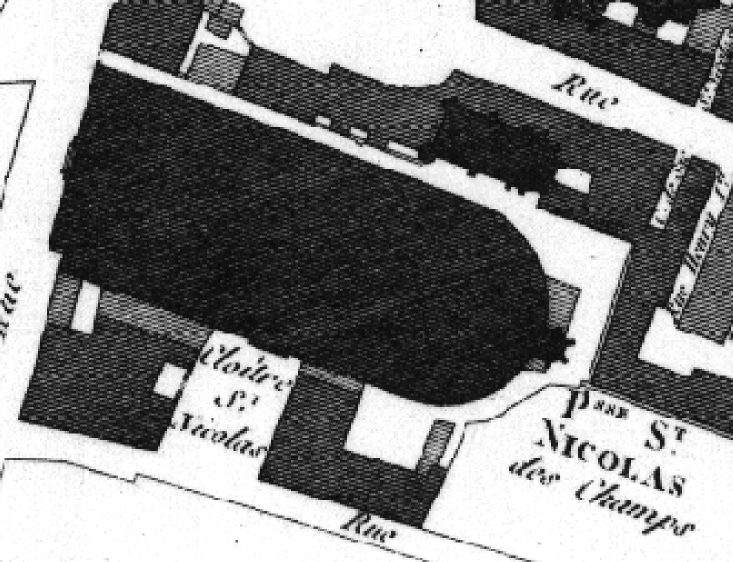
\includegraphics[width=\textwidth]{raster.png}
                \caption{L'�glise Saint Nicolas des Champs dans plan de Verniquet num�ris�.}
                \label{fig:verniquet_raster}
        \end{subfigure}%
~~~~
	\begin{subfigure}[b]{0.4\textwidth}
                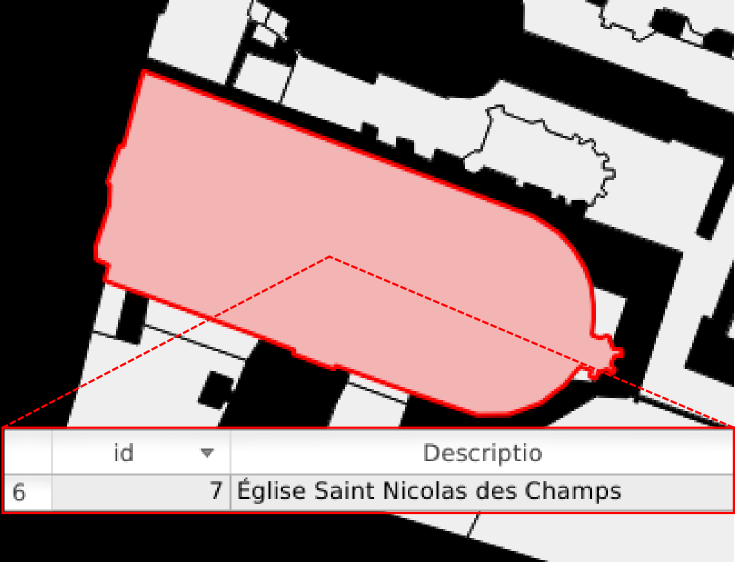
\includegraphics[width=\textwidth]{vecteur.png}
                \caption{Repr�sentation vecteur de la m�me �glise.}
                \label{fig:verniquet_vecteur}
        \end{subfigure}%
         \caption{Les deux modes de repr�sentation de l'information g�ographique.
Raster en (a), vecteur en (b).}
	\label{fig:vecras}
\end{figure}



\subsubsection{Int�grer une information g�ohistorique explicite}
On consid�re les cartes, plans et mappes, ainsi que les repr�sentations iconographiques d'un espace ou d'un monument, comme des sources g�ohistoriques explicites.
Les reliques, vestiges arch�ologiques ou traces sur le terrain, peuvent �galement �tre consid�r�es comme explicites, leur localisation pouvant �tre acquise par mesure directe (en particulier par relev� GPS).
Nous ne consid�rons pas ici le cas des sources iconographiques qui sont, aux �poques consid�r�es, g�n�ralement des vues en perspectives de b�tis, de lieux ou de sc�nes de vies et qui n�cessitent d�s lors des donn�es 3D pour �tre recal�es.
La constitution de donn�es 3D sur l'espace pass� est probl�matique, en raison de la pauvret� des sources. En effet, peu de sources anciennes permettent de reconstruire des �l�ments en volumes et plus rares encore sont celles qui repr�sentent ces �l�ments avec r�alisme.

\myparagraph{G�or�f�rencement}
% \newglossaryentry{SCR}{name={Syst�me de coordonn�es}, description = {\emph{Le Syst�me de coordonn�es est un syst�me de r�f�rence permettant d'exprimer la position d'un objet dans ses 2 ou 3 dimensions.} Un syst�me de coordonn�es peut �tre sph�rique, permettant alors de positionner un �l�ment � la surface du globe terrestre.
%Il peut s'agir �galement d'une projection cartographique plane}}
\subparagraph{}
Les sources cartographiques constituent un �l�ment central dans la construction d'une d�marche qui vise � reconstituer la morphologie d'un espace pass� et d'en donner une repr�sentation globale.

Afin de pouvoir les confronter de mani�re critique � d'autres sources et d'autres donn�es spatiales, il est n�cessaire d'assigner une localisation pr�cise dans l'espace g�ographique aux cartes et plans.
Cette op�ration, nomm�e \emph{g�or�f�rencement} n'est pas propre aux sources historiques mais elle constitue une �tape cruciale dans la constitution d'un SIG historique pour lequel une grande part des donn�es spatiales provient de cartographies anciennes \citep{Rumsey2002}.
\subparagraph{}
L'op�ration de g�or�f�rencement implique tout simplement la tentative de faire correspondre, et donc de superposer dans un rep�re g�ographique, le plus exactement possible, les objets g�ographiques communs � la carte ancienne et � la carte contemporaine. Pour ce faire, la m�thode habituellement adopt�e \citep{Rumsey2002} consiste � placer des \emph{points de contr�le}, g�n�ralement de fa�on manuelle, dans la carte num�ris�e sous forme raster une carte.
� chaque point de contr�le est alors li� un second point situ� dans un r�f�rentiel spatial muni d'un syst�me de coordonn�es de r�f�rence choisi au pr�alable.
Les nombreuses bases de donn�es g�ographiques actuellement � disposition servent souvent de r�f�rentiels, les points de contr�les �tant plac�s sur des �l�ments du paysage (point culminant, tour, croisement de rues, etc.) pr�sent � la fois dans le r�f�rentiel et dans la carte.
Quant au g�or�f�rencement, il repose sur l'application de m�thodes de transformation math�matiques permettant, � partir des points de la carte ainsi associ�s, d'assigner une coordonn�e � chaque point de la carte raster\citep{Grosso2010}.
\subparagraph{}
Comme le note \citep[p. 5]{Rumsey2002}, le g�or�f�rencement parfait de cartes anciennes sur un r�f�rentiel actuel est souvent impossible.
D'abord, les syst�mes de coordonn�es utilis�s dans les cartes anciennes ne correspondent plus � ceux utilis�s actuellement, et sont souvent difficiles � reconstituer.
De plus, la pr�cision g�om�trique des plans anciens est variable, en raison des techniques de lev� ou encore de la pr�cision des instruments de mesures g�od�siques utilis�s.
Les biais introduits par les cartographes ayant trac� la carte influent �galement sur la pr�cision g�om�trique des informations qu'elle contient.
Ainsi, sur la carte de Cassini dress�e pour l'ensemble de la France entre $1747$ et $1789$ \footnote{Les relev�s sont termin�s au moment de la R�volution, mais la carte ne sera enti�rement �dit�e qu'en 1815.}, la taille et le nombre de certains symboles peuvent affecter la disposition des �l�ments, en provoquant, par exemple, le d�placement du trac� d'une rivi�re au profit du toponyme d'un village \citep[p. 3]{GeopeupleL231}.
Enfin, les conditions de conservation peuvent d�former une carte ancienne, notamment si son support est sensible � l'humidit� (bois, toile, papier,etc.).
 
\myparagraph{Vectorisation}
La seconde m�thode d'int�gration d'une information g�ohistorique explicite dans un SIG consiste � transformer les objets g�ographiques repr�sent�s dans la carte en objets vecteurs~: il s'agit de la \emph{vectorisation}.
Cette �tape succ�de au g�or�f�rencement et permet d'assigner � chaque objet g�ographique identifi� dans la carte une primitive g�om�trique, des informations s�mantiques sous forme d'attributs ainsi qu'une identit�.
Cette identit�, implicite lorsque l'objet est saisi, peut �tre explicit� par exemple � l'aide d'un identifiant unique.
La vectorisation d'une carte ancienne offre plusieurs avantages~:
\begin{itemize}
 \item Elle permet d'extraire l'information s�mantique contenue dans la carte et de s'abstraire du style cartographique qui lui est associ�e.
 \item La s�paration des composantes de l'information spatiale permet de nombreux traitements automatiques par un outil SIG (croisements attributaires, requ�tes spatiales, s�lection,etc.)
\end{itemize}

Tout comme le g�or�f�rencement, la vectorisation de cartes est loin d'�tre une t�che anodine.
En premier lieu, elle implique des op�rations de pr�cision qui peuvent se r�v�ler longues en raison du nombre d'objets, ce qui explique en partie la raret� des bases historiques vectorielles~\citep{Rumsey2002}.
En second lieu, la vectorisation d'une carte implique d'identifier des objets au sein d'une carte, c'est � dire � assigner une identit� particuli�re � une zone de l'espace.
Dans les cartes historiques cette assignation peut poser probl�me.
En effet, dans une carte r�cente il peut �tre possible de comparer une repr�sentation cartographique avec l'espace r�el et aider ainsi la vectorisation, ce qui est impossible lorsqu'il s'agit d'une carte historique.
En cons�quence la carte ancienne devient le seul t�moin d'un objet g�ographique dont l'identification n'est pas toujours ais�e.


\subsubsection{Int�grer une information g�ohistorique implicite}
Les sources d'information g�ographique habituellement d�finies comme ''implicites'' sont constitu�es par l'ensemble des ressources portant une information spatiale qu'il n'est pas possible de localiser directement.
La forme de ces informations et la difficult� de leur localisation varient largement~: l'adresse postale d'un individu ou l'itin�raire d'un voyageur sont toutes deux des informations implicites et pourtant tr�s diff�rentes.
%Les donn�e statistiques sont �galement implicites lorsqu'elles font r�f�rence � un ph�nom�ne spatial et peuvent donc �tre cartographi�es. La cartographie des donn�es statistiques ne sera pas abord�e ici, en raison notamment d

\myparagraph{G�ocodage}
Conceptuellement proche mais techniquement diff�rent des op�rations de g�or�f�rencement, le \emph{g�ocodage} consiste � placer une donn�e spatiale implicite dans un rep�re g�ographique absolu \citep{Goldberg2007} en lui attribuant une coordonn�e g�ographique.
Tr�s utilis�e dans diverses disciplines, cette op�ration permet~:
\begin{itemize}
 \item D'int�grer une information s�mantique dans un r�f�rentiel spatial en vue de croisements avec d'autres informations.
 C'est notamment le cas des adresses, qui, une fois localis�es, peuvent permettre de mettre en relations divers sources dont elles constituent le lien (par exemple pour des habitations parisiennes~: des actes notari�s, des recensements, des calepins cadastraux,etc.
 \item De cartographier ces informations et �ventuellement de faire appara�tre des relations jusqu'alors invisibles \citep{Gauthiez2010}.
\end{itemize}
Les m�thodes de g�ocodages sont tr�s diverses et d�pendent fortement du cas d'application et aboutissent au d�veloppement de m�thodes \emph{ad-hoc}, dont on pourra trouver un �tat de l'art d�taill� dans \citep{Goldberg2007}.
Depuis quelques ann�es cependant, les diff�rentes propositions de m�thodes de g�ocodage tendent � s'appuyer sur des 
index g�ographiques en ligne tels Geonames\footnote{http://www.geonames.org/} ou Pleiades\footnote{http://pleiades.stoa.org/}.

% 
% Les informations spatiales disponibles sous forme textuelles sont particuli�rement h�t�rog�nes et leur localisation peut �tre difficilement identifiable. Ce peut �tre le cas lorsque les informations de localisation sont vagues ou bien qu'elles sont relatives � d'autres lieux \citep{Eide2013}, ou bien encore lorsque l'orthographe d'un nom varie. Un nombre croissant de m�thodes de g�ocodage permettent de prendre en compte les incertitudes de ces donn�es
 
%
%
%\begin{center}
%\fcolorbox{black}{white}{
%  \begin{minipage}[t]{0.9\textwidth}
%\begin{center}
% \textbf{R�sum� de la section}
%\end{center}
%En d�finissant les SIG historiques par rapport � une utilisation plus classique de ces syst�mes (gestion du territoire, urbanisme, etc.), nous avons mis en lumi�re deux besoins particuliers des historiens.
%Premi�rement, les SIG constituent un outil performant de croisement et de partage de donn�es historiques spatiales, permettant aux chercheurs de mettre en relation des donn�es dont l'acc�s et l'exploitation peuvent �tre difficiles.
%Deuxi�mement, par leur capacit� � stocker des donn�e spatiales h�t�rog�nes, les SIG constituent un outil de choix pour traiter des donn�es spatio-temporelles.
%\subparagraph{}
%Cependant, l'utilisation de SIG n�cessite des traitements sp�cifiques sur l'information g�ohistorique en vue de son int�gration.
%Le g�or�f�rencement, la vectorisation de plans ou le g�ocodage de donn�es constituent trois outils de base permettant d'int�grer une telle information.
%En ajoutant des �tapes de traitement ainsi qu'en utilisant des outils peu adapt�s \emph{a priori} pour manipuler des donn�es historiques, le risque d'accumulation d'erreurs dans les donn�es et dans leur traitement augmente.
%  \end{minipage}
%} 
%\end{center}

\section{Les difficult�s dues aux imperfections de l'information g�ohistorique}
\label{section:imperfections}
Nous venons de voir que les SIG constituent un outil performant de croisement et de partage de donn�es historiques spatiales, permettant aux chercheurs de mettre en relation des donn�es dont l'acc�s et l'exploitation peuvent �tre difficiles. Par leur nature, les SIG n�cessitent des traitements sp�cifiques pour int�grer et traiter des informations g�ohistoriques. Le g�or�f�rencement, la vectorisation de plans et le g�ocodage constituent les trois outils de base permettant ces op�rations. Cependant, tout en �tant tr�s performante, ces op�rations sont loin d'�tre anodines. En int�grant une suite de techniques con�ues et d�velopp�es pour des traitements fond�s sur l'observation directe des sources et des terrains, elles risquent de d�former les informations port�es par les sources historiques dont la sp�cificit� est avant tout li�e � leurs imperfections. L'information g�ohistorique, comme toute information, est en effet toujours entach�e d'imperfections~\citep{Plewe2002}.
La principale raison, d�j� �voqu�e pour la repr�sentation cartographique, r�side dans l'impossibilit� de saisir la complexit� d'�l�ments qui permettent de saisir un ph�nom�ne dans la totalit� de ses dimensions. Ces imperfections ont �t� largement �tudi�es et sont notamment d�crites par~\cite{BouchonMeunier1995} qui en a propos� une typologie fond�e sur trois classes~:
\begin{itemize}
 \item \textbf{L'incertitude}~: Une information est dite incertaine lorsque on a un doute sur sa validit�.
Par exemple, le t�moin d'un vol de voiture peut expliquer � la police qu'il ''pense que la voiture �tait verte''.
L'information sur la couleur de la voiture est incertaine~: elle est tr�s probablement verte, mais ce n'est pas certain.
 \item \textbf{L'impr�cision}~: Une information impr�cise aboutit � l'impossibilit� de d�finir clairement des limites � une ou plusieurs entit�s.
Ces limites peuvent �tre mal connues en raison de manques dus aux appareils de mesure (par exemple un thermom�tre pr�cis � 1�C pr�s).
Une impr�cision appara�t �galement lorsque les limites d'une entit� sont flexibles car d�sign�es par des termes vagues.
 Ce peut �tre le cas �galement quand les limites sont flexibles, soit parce qu'elles sont d�finies de fa�on vague, soit parce qu'elles sont proviennent 
\item \textbf{L'incompl�tude}~: Il est possible qu'une information parvienne de fa�on incompl�te, soit parce qu'une partie est manquante, soit parce qu'elle ne couvre pas l'int�gralit� du ph�nom�ne repr�sent�.
\end{itemize}
Ces trois types d'imperfections se retrouvent � diff�rents instants de l'acquisition, la repr�sentation et l'analyse de l'information g�ohistorique.
Dans cette section, nous proposons de mettre en lumi�re ces imperfections et de les mettre en rapport avec le processus de repr�sentation d'un espace ancien abord� dans la section \ref{section:carto_ancienne}.
\subparagraph{}
Les imperfections des informations spatiales repr�sent�es au sein des SIG sont aujourd'hui bien connues et identifi�es au travers de plusieurs taxonomies visant � classifier les types, les causes et les effets de chaque imperfection \citep{Fisher1999, Klir1995,Atkinson2002, Fisher2005}.
Lorsqu'il s'agit d'informations g�ohistoriques, spatiales mais �galement temporelles, issues de sources d�cal�es temporellement, il devient n�cessaire d'adapter les approches et les mod�les existants.
Au cours de la derni�re d�cennie, plusieurs chercheurs ont �labor� des propositions visant � sp�cialiser les mod�les existants pour le traitement de donn�es g�ohistoriques \citep{Plewe2002, Leyk2005, DeRunz2008}.
En nous inscrivant � notre tour dans cette optique, � partir de l'analyse du processus d'int�gration des informations g�ohistoriques dans un SIG, nous avons essay� de proposer un mod�le adapt� pour l'analyse des transformations morphologiques de l'espace urbain.

\myparagraph{Incertitude et imperfection}
Notons d�s � pr�sent que les mod�les d'imperfection de l'information spatiale rassemblent les diff�rents types d'imperfections des donn�es et de l'information spatiale sous le terme d'\emph{incertitudes}.
Cependant, de la m�me mani�re que \cite{DeRunz2008}, nous lui pr�f�rerons ici le terme d'\emph{imperfection} issue de la classification de \cite{BouchonMeunier1995}.
Le sens de l'incertitude pour \cite{BouchonMeunier1995} et pour les mod�les tels celui de \cite{Fisher2005} varient sensiblement.
En effet, pour \cite{Fisher2005} l'incertitude est le concept qui coiffe l'ensemble des d�fauts qui affectent l'information, tandis la validit� de l'information est plut�t li�e au concept d'erreur.

\subsection{Le processus d'int�gration d'une information g�ohistorique}
Nous avons pour l'instant parl� des imperfections qui affectent l'information g�ohistorique de fa�on g�n�rale, sans en identifier les causes, les types et les effets.
La premi�re �tape est alors d'identifier les causes de ces imperfections.
Dans les sections pr�c�dentes, diff�rentes imperfections sont apparues~: imperfections des sources historiques, de l'information qu'elles contiennent ou bien encore de sa repr�sentation au sein d'un SIG.
Ces divers g�n�rateurs d'informations imparfaites se trouvent r�partis � diff�rents instants de l'int�gration d'informations g�ohistoriques dans un SIG.
\myparagraph{Les �tapes du processus}
D'autres recherches ont permis d'individualiser les diff�rents moments durant lesquels des imperfections apparaissent � l'int�rieur du processus d'int�gration d'informations g�ohistoriques dans un SIG.
Ainsi, on distingue classiquement trois �tapes dans ce processus \citep{Fisher1999, Longley2005}, d�crites dans la figure \ref{fig:imperfection}.
La proximit� avec la figure \ref{fig:comm_carto_traces} sur la communication cartographique est naturelle~: il s'agit d'une forme particuli�re de repr�sentation d'informations spatiales. \cite{Plewe2002} fournit une description plus d�taill�e de chacune des �tapes du processus.
Ainsi, d'apr�s lui, le processus serait constitu� de la cha�ne d'�tats suivants~:

\begin{itemize}
 \item D'abord, une part de la r�alit� est \textbf{conceptualis�e}.
Cette �tape consiste � identifier diff�rentes entit�s g�ographiques qui constituent la r�alit� d'un lieu � une �poque donn�e, selon leur nature (voir le paragraphe \ref{paragraph:entite}).
L'identification de ces entit�s construit leur \emph{�tendue id�ale} (\emph{ideal extent}), c'est � dire la repr�sentation mentale des trois dimensions qui composent l'�tendue de l'entit�.
 \item Ensuite, les entit�s identifi�es sont \textbf{mesur�es} par le biais de diff�rentes m�thodes (observation, g�n�ralisation, classification, interpr�tation ou encodage), ce qui permet de construire leur repr�sentation sous la forme de donn�es manipulables par un SIG.
Cette op�ration permet de cr�er l'\emph{�tendue �valu�e} (\emph{asserted extent}) de l'entit�, c'est � dire la transformation de l'entit� conceptuelle en donn�e concr�te dont le propri�t�s ont �t� mesur�es.
  \item Enfin, la derni�re phase d'\textbf{analyse} permet de construire de nouvelles entit�s � partir de celles d�j� connues.
G�n�ralement, ces entit�s sont plus pr�cis�ment d�finies que les donn�es initiales \citep{Plewe2002}.
Par exemple, une personne localis�e par une �tape de g�ocodage aura une �tendue plus compl�te que la donn�e d'origine dont on ne connaissait pas la localisation.

\end{itemize}

\begin{figure}[ht]
	\centering
		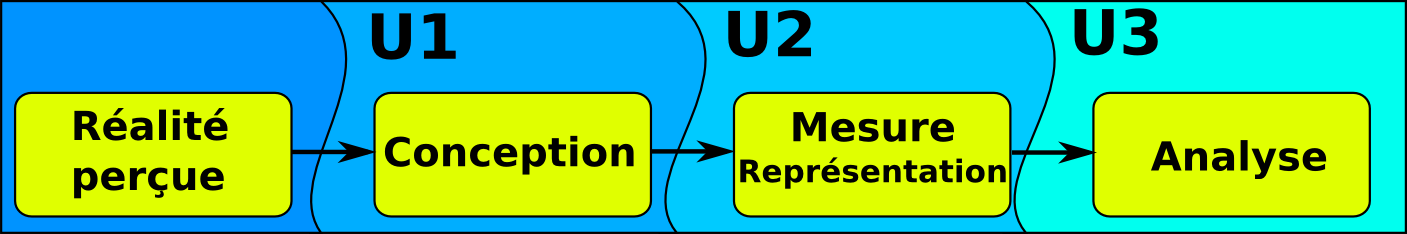
\includegraphics[width=0.8\textwidth]{uncertainty.png}
	\caption{Sch�ma des diff�rents filtres (U1,U2,U3) d�formant la r�alit�e per�ue et repr�sent�es dans un SIG.
Chaque filtre g�n�re des imperfections diff�rentes affectant l'information spatiale transmise.}
	\label{fig:imperfection}
\end{figure} 

\myparagraph{Sources des imperfections}
\cite{Longley2005} identifient trois principales causes menant � la d�gradation de l'information spatiale. \cite{Leyk2005}, en l'adaptant au cas o� l'information provient de sources historiques, les pr�sentent comme tel~:
\begin{itemize}
 \item Les \textbf{Imperfections orient�es production}~: Il s'agit des diff�rentes imperfections inh�rentes � l'utilisation de sources historiques.
Pour \cite{Leyk2005}, il s'agit des erreurs des sources~: les erreurs de position et les erreurs dans les attributs des donn�es\citep{Atkinson2004}.
Ainsi, les erreurs de lev�s des cartographes ou l'impr�cision de leurs mesures se retrouvent invariablement au sein des sources.
 \item Les \textbf{Imperfections orient�es transformations}~: Ce sont les diff�rentes imperfections qui r�sultent de la transformation de l'information contenue dans les sources en donn�e utilisable, sous forme vecteur ou raster.
Ainsi, le g�or�f�rencement de cartes anciennes d�forme l'espace, et la vectorisation ne permet que de saisir partiellement le contenu de la carte.
 \item Les \textbf{Imperfections orient�es application}~: Il s'agit cette fois des imperfections dues � la comparaison des donn�es issues de diff�rentes sources et � leur confrontation � l'espace pr�sent.
Les mauvaises interpr�tations du contenu des sources dues au manque d'informations sur les pratiques des cartographes en sont un exemple.
\end{itemize}

Ces diff�rentes sources d'imperfections se retrouvent de fait sur le sch�ma \ref{fig:imperfection}.
En effet, la transition entre les diff�rents �tats de l'information g�ohistorique est effectu�e par l'application  de plusieurs filtres (d�nomm�s U1, U2 et U3) qui s'appliquent les uns apr�s les autres.
Ces filtres d�forment la r�alit� de fa�on progressive, d�gradant et modifiant l'information initiale.
\begin{itemize}
 \item Le premier filtre \textbf{U1} correspond � la perception de la r�alit� qui aboutit � la repr�sentation mentale d'un espace \citep{Bailly1985}.
Lorsque la r�alit� pass�e n'est plus perceptible que par des sources historiques, le filtre U1 g�n�re les imperfections orient�es production.
 \item Le second filtre \textbf{U2} correspond � la transition entre l'entit� conceptuelle et l'entit� mesur�e.
Sur des sources historiques, la mesure est effectu�e par le g�or�f�rencement, le g�ocodage et la vectorisation.
Le filtre U2 est source d' imperfections de transformation.
 \item Enfin, les donn�es g�ohistoriques sont interpr�t�es au sein d'une grille d'analyse, cr�ant un dernier filtre \textbf{U3}.
Cette fois, ce sont les imperfections orient�es application qui apparaissent.
\end{itemize}

\subsection{Types d'imperfections de l'information g�ohistorique}
En montrant le processus d'int�gration de l'information g�ohistorique depuis des sources, nous avons mis en lumi�re les diff�rents �v�nements qui d�gradent l'information.
Cependant, il faut encore pr�ciser quelles sont exactement les types d'imperfections qui peuvent affecter cette information.
Dans le cas de l'information spatiale, la taxonomie de \cite{Fisher2005} fait �cole car elle associe � chaque type d'imperfection un formalisme math�matique permettant de la repr�senter.
Sur ces bases, \cite{DeRunz2008} a propos� une taxonomie adapt�e � l'information arch�ologique.
Cette taxonomie s'adaptant � nos donn�es, nous proposons de l'utiliser pour identifier et traiter l'imperfection de l'information g�ohistorique dans cette th�se.
La figure \ref{fig:redunz} pr�sente cette taxonomie.
Nous d�taillons ensuite les diff�rents types d'imperfection en les sp�cialisant sur le cas des donn�es g�ohistoriques issues de cartes anciennes.

\begin{figure}[ht]
	\centering
		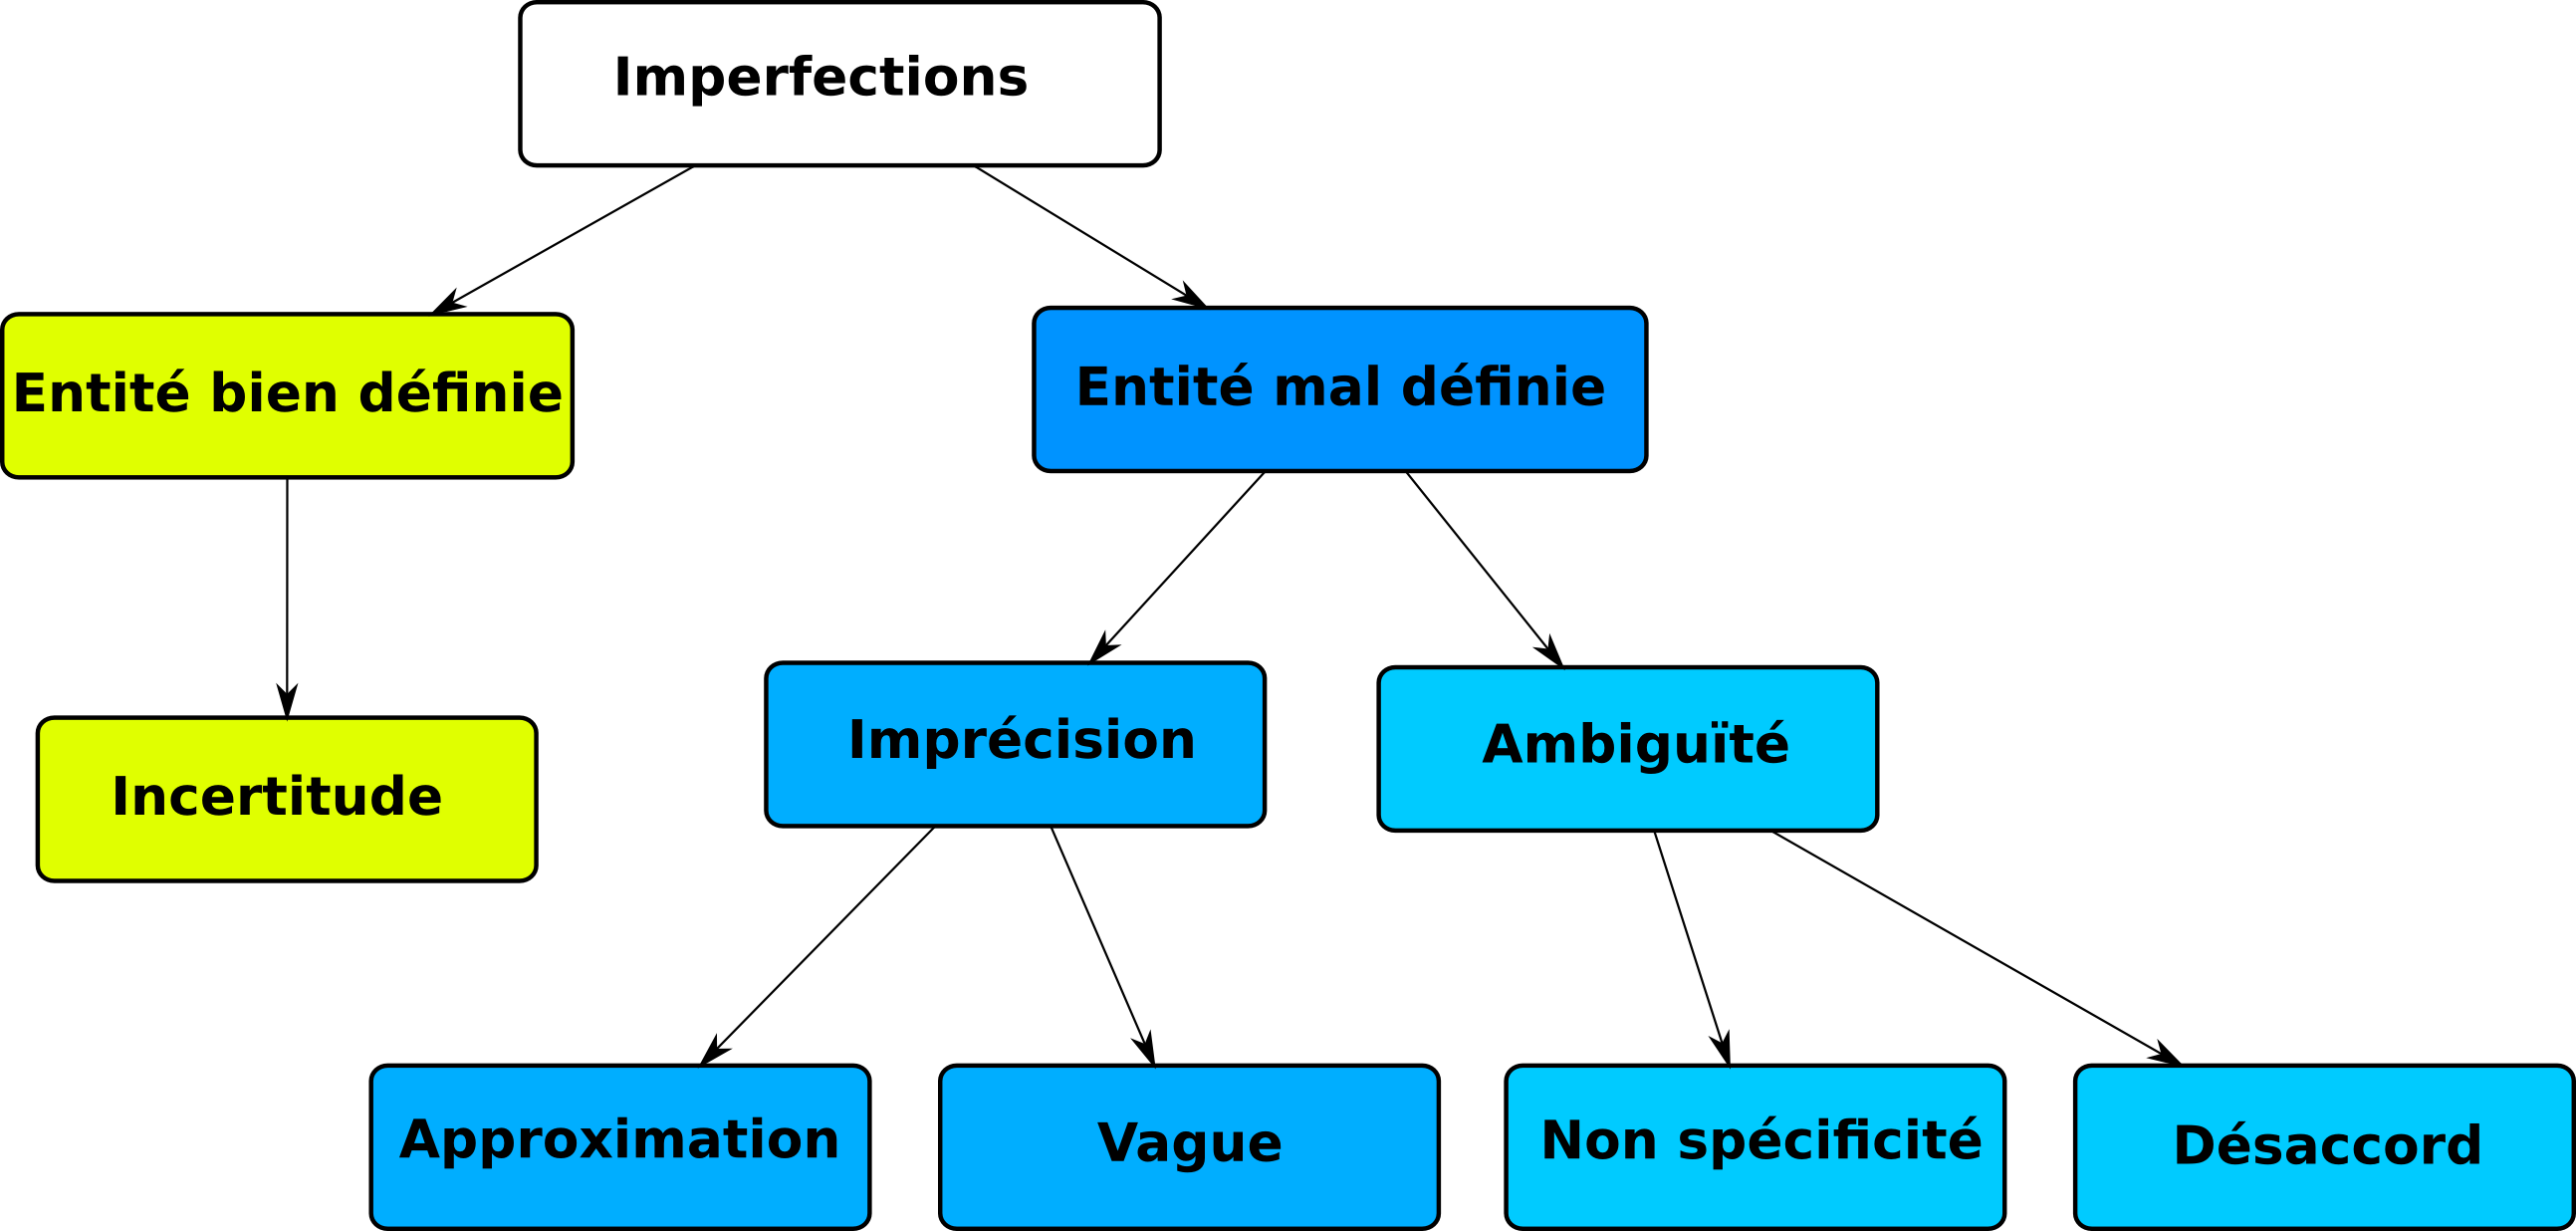
\includegraphics[width=0.8\textwidth]{derunz.png}
	\caption{Taxonomie des imperfections de l'information g�ohistorique, d'apr�s \cite{DeRunz2008}}
	\label{fig:redunz}
\end{figure} 

\subsubsection{D�tails de la taxonomie}

\myparagraph{Qualit� de d�finition d'une entit�}
Une premi�re distinction est faite selon la qualit� de d�finition de l'entit� g�ohistorique consid�r�e.
En effet, le premier probl�me qui se pose lors de l'�tape de conceptualisation est la construction des limites de l'entit�, ou, pour reprendre \cite{Fisher2005}, de l'affectation d'une classe � chaque portion de l'espace.
Une entit� est bien d�finie lorsque qu'elle est sp�cifi�e de mani�re \emph{compl�te, pr�cise et unique} \citep{DeRunz2008}.
Afin d'illustrer chaque cat�gorie d'imperfection, nous nous appuierons sur l'exemple de la rue \emph{Au Maire} illustr�e dans la figure \ref{fig:aumaire}.
Chaque type d'imperfection peut s'appliquer � toute une entit� ou seulement � l'une de ses trois composantes.

\myparagraph{Incertitude}
M�me lorsqu'une entit� est bien d�finie, il est possible qu'elle soit incertaine. Pour se rattacher au sens fix� par \cite{BouchonMeunier1995} (\ref{section:imperfections}), il peut s'agir d'une entit� dont la validit� d'au moins une partie de son �tendue est mise en doute.
\subparagraph{}
Reprenons le cas du champ de bl� dont l'information sur l'emprise spatiale et le type de culture est issue d'un plan ancien.
Son �tendue �valu�e correspond donc spatialement � son emprise sur la carte, sa p�riode de vie � la date du plan et sa s�mantique est donn�e par son type de culture.
Cette derni�re information peut �tre soit fausse, soit vraie. Elle peut �tre affect�e par diverses erreurs et la source en elle-m�me peu fiable \citep[p. 28]{DeRunz2008}.
D�s lors, la validit� du type de culture \emph{bl�} peut �tre mise en doute, bien que le champ soit une entit� bien d�finie.


\myparagraph{Impr�cision}
Une entit� peut �tre mal d�finie lorsque la sp�cification de ses �l�ments constitutifs n'est que partielle.
Plus pr�cis�ment, l'impr�cision appara�t d�s lors qu'il est impossible de fixer des limites bien d�finies pour une entit� ou pour un de ses �l�ments, rendant impossible sa cat�gorisation simple dans une classe unique et menant � la n�cessit� de classer les limites comme floues.
Reprenant \cite{BouchonMeunier1995}, cite{DeRunz2008} sp�cialise l'impr�cision en deux sous-cat�gories~: le vague et l'approximatif.

\begin{itemize}
 \item Le fait qu'une entit� soit d�finie de fa�on vague r�sulte de l'utilisation de termes du langage naturel subjectifs ou flexibles \citep[p. 29]{DeRunz2008}.
Par exemple, on peut dire que l'�glise Saint Nicolas des champs est ''proche de'' ou bien m�me ''� l'entr�e ouest'' de la rue \emph{Au Maire} et ''au nord'' de celle-ci.
Ces trois termes permettent de localiser l'�glise par rapport � la rue de fa�on indirecte, mais uniquement de fa�on vague.
Cette description ne permet pourtant pas de localiser de mani�re pr�cise l'�glise car chacun des termes ne d�finit que des relations spatiales variables et subjectives.
 \item Une entit� est d�finie de fa�on approximative lorsque ses limites ne peuvent pas �tre clairement fix�es, en cons�quence de quoi l'entit� englobe des �l�ments qui ne lui appartiennent que partiellement.
Par exemple, la rue \emph{Au Maire} a �t� allong�e en 1833 par une perc�e � l'Est.
Pour autant, cette perc�e n'est pas un �v�nement instantan� mais un certain temps s'est d�roul� entre la d�cision d'ouverture et la fin des travaux.
La date donn�e est donc une approximation de la v�ritable tranche temporelle qui correspond � la dur�e de l'op�ration.
\end{itemize}

\myparagraph{Ambigu�t�}
L'ambigu�t� est induite quand une entit� appartient, int�gralement ou en partie, � plusieurs cat�gories possibles.
Pour \cite{DeRunz2008}, un tel probl�me r�sulte soit d'un manque de sp�cificit� de la d�finition de l'entit�, soit d'un d�saccord entre plusieurs d�finitions.
Dans les deux cas, le probl�me peut �tre d� soit � des divergences entre des avis d'experts, ou bien directement par des incoh�rences dans les sources de donn�es.
\begin{itemize}
 \item Une entit� pr�sente un manque de sp�cificit� lorsque plusieurs classes peuvent lui correspondre.
La rue \emph{Au Maire} est en partie construite sur un ancien cul-de-sac, parfois d�nomm� \emph{Cul-de sac de Rome} ou \emph{Passage de Rome}, bien que sa structure n'ai pas chang�.
Il est clair ici que deux classe de voies (cul-de-sac et passage) dont le sens est tr�s diff�rent peuvent s'appliquer � la m�me entit�.
Il faut remarquer que ce manque de sp�cificit�, du moins lorsque l'on travaille avec des plans anciens, r�sulte en partie des diff�rences d'�chelles et de niveaux d'interpr�tation des informations qu'ils contiennent.
 \item Enfin, une information sur une entit� peut rentrer en conflit avec une autre.
D�s lors, une m�me entit� peut poss�der plusieurs valeurs pour chacun de ses �l�ments constitutifs qui sont en d�saccord.
Plusieurs d�finitions d'une entit� peuvent �galement �tre en conflit, par exemple lorsque les avis de deux experts divergent.
\end{itemize}

\subsubsection{Incompl�tudes}
Enfin, \cite{DeRunz2008} sp�cifie deux autres types d'imperfections qui se diff�rencient substantiellement des autres, � savoir les lacunes et les absences.
Ces deux types sont des sous-cat�gories de la notion d'incompl�tude abord�e par \cite{BouchonMeunier1995}.
L'absence d�signe le fait qu'il manque des informations pour d�crire compl�tement une entit�.
Par exemple, m�me si l'on sait que la rue \emph{Au Maire} existait en 1280, on ne dispose pas de sources sur son emprise spatiale.
Des trois �l�ments espace-temps-s�mantique qui participent � la d�finition de l'entit� rue, l'espace est dans ce cas absent.
Les lacunes ajoutent une dimension hi�rarchique � la notion d'incompl�tude.
En effet, une entit� est lacunaire lorsqu'elle est compos�e de plusieurs entit�s dont certaines sont inconnues.
\subparagraph{}
L'incompl�tude est sans doute le type d'imperfection le plus r�pandu dans les informations g�ohistoriques.
En effet, ces informations sont issues de sources partielles, �parses et r�guli�rement incompl�tes.
Ainsi, aucun plan ne d�crit exhaustivement un espace, et chacun d�crit de fa�on diff�rente un m�me espace.
Enfin, comme toute source d'information, les plans ne donnent qu'un aper�u d'un espace pendant une courte p�riode.
Entre ces p�riodes de temps, l'�tat de l'espace doit �tre suppos� inconnu.
%
%\begin{center}
%\fcolorbox{black}{white}{
%  \begin{minipage}[t]{0.9\textwidth}
%\begin{center}
% \textbf{R�sum� de la section}
%\end{center}
%Dans cette section, nous avons d�taill� la nature de l'imperfection de l'information g�ohistorique et de ses impacts sur les entit�s g�ographiques mesur�es, acquises et manipul�es au sein d'un SIG.
%En nous appuyant sur la taxonomie des imperfections de l'information arch�ologique mise en place par \cite{DeRunz2008}, nous avons d�crit chaque cat�gorie d'imperfection inh�rentes aux informations g�ohistoriques issues de sources cartographiques.
%
%  \end{minipage}
%} 
%\end{center}

\section{�tat de l'art des SIG utilis�s en histoire}
\label{subsection:currgis}
\myparagraph{Diffusion de donn�es historiques}
Nous avons identifi� la diffusion de donn�es, c'est � dire la mise � disposition de donn�es de mani�re large et syst�matique, comme un des facteurs importants de l'engouement des sciences sociales envers les SIG.
Les donn�es g�ographiques ainsi diffus�es sont g�n�ralement associ�es � des plateformes de webmapping permettant d'acc�der de fa�on plus rapide et plus intuitives aux donn�es voulues.
�tant donn� le co�t de d�veloppement d'un site web d�di� � la diffusion de telles donn�es, on y retrouve essentiellement des plateformes mises en place au niveau d'un �tat.
C'est par exemple le cas des SIG historiques de Grande Bretagne (GBHGIS) \citep{GBHGIS} et des �tats-Unis (NHGIS) \citep{NHGIS} portant respectivement sur l'ensemble des deux pays.
De tels SIG sont alors d�di�s � la diffusion � grande �chelle de donn�es d�mographiques et sociales socio-�conomiques spatialis�es, notamment les recensements du pays � diff�rentes dates~: ce sont des index g�ohistoriques ou \emph{historical gazetteers}.
\subparagraph{}
D'autres SIG visent d'avantage la diffusion de cartes anciennes et se constituent en atlas historiques en ligne.
Ces outils mettent � disposition du public des collections de cartes historiques, g�n�ralement topographique et sous forme raster \citep{Rumsey2012}.
Le SIG historique ALPAGE \citep{ALPAGE} est un cas particulier de SIG d�di� � la diffusion de donn�es.
En effet, les donn�es diffus�es par le SIG ALPAGE sont, pour la majorit�, des informations spatiales vectoris�es � partir de divers documents anciens.
S'il ne s'agit pas d'un index g�ohistorique comparable aux SIG pr�c�dents, l'objectif d'ALPAGE ne se limite pas � la diffusion de cartes anciennes.
La mise � disposition de donn�es topographiques (cadastre napol�onien vectoris�, limites anciennes,etc.) permet de fournir, en plus d'informations sur un espace (en l'occurrence, Paris), des donn�es manipulables par des outils SIG exterieurs dans des buts d'analyse spatiale ou de g�ocodage.

\myparagraph{Repr�sentation visuelle}
La repr�sentation visuelle de donn�es historiques constitue �galement un des besoins de la recherche en histoire.
Il n'est donc pas �tonnant de retrouver des outils de visualisation cartographique dans la majorit� des SIG historiques pr�sent�s dans le tableau \ref{table:exgis}.
Si des outils de repr�sentation visuelle sont syst�matiquement disponibles, la nature de ces outils d�pend des objectifs du SIG~: soit il s'agit de communiquer les r�sultats d'une �tude historique, soit il s'agit de visualiser des donn�es historiques dans un but de diffusion.
\subparagraph{}
Diff�rents moyens sont alors utilis�s.
Lorsqu'il s'agit de communiquer des r�sultats de recherche, le SIG historique peut simplement mettre � disposition des cartes cr��es pour les besoins de l'�tude, comme par exemple pour le projet \emph{Valley of the Shadow} \citep{VALLEY}.
Plus souvent, la mise en place d'un outil de \emph{webmapping} permet de communiquer au sein d'un seul outil l'ensemble des donn�es cr��es ou assembl�es au cours de l'�tude.
La diffusion de donn�es s'appuie �galement largement sur de tels outils, permettant un acc�s plus intuitif � des donn�es spatiales.
\subparagraph{}
Bien qu'il s'agisse �galement d'un index g�ohistorique, l'outil en ligne GAPVIS \citep{GAPVIS} vise un but diff�rent.
L'objectif de ce SIG historique est de cartographier les lieux et les relations entre lieux d�crits au sein de r�cits anciens.
� partir de textes de livres anciens issus de \emph{Google Books}, les lieux sont automatiquement d�tect�s et g�ocod�s � l'aide de l'index g�ographiques web externes Pl�iades\footnote{http://pleiades.stoa.org/}.

\myparagraph{Gestion des imperfections}
Nous l'avons vu, les imperfections des informations g�ohistoriques sont nombreuses et se trouvent � toutes les �tapes de l'int�gration de donn�es dans un SIG.
la gestion de ces imperfections devient primordiale lorsque l'on traite de donn�es fortement imparfaites dont les d�fauts peuvent mener � une lecture erron�e.
Plus radicalement, de trop fortes imperfections peuvent s'accumuler pour rendre le ph�nom�ne retranscrit illisible.
Pourtant, rares sont les SIG historiques qui mod�lisent explicitement les diff�rentes imperfections des donn�es.
\subparagraph{}
La majeure partie du temps, les donn�es font l'objet de pr�-traitements de fa�on � r�duire ou �liminer ces imperfections.
Les donn�es raster -g�n�ralement des cartes anciennes- sont g�or�f�renc�es en amont de leur mise � disposition.
Cette op�ration aborde par nature certaines imperfections des plans, notamment les erreurs g�om�triques qui emp�chent un recalage parfait de ces plans sur un r�f�rentiel r�cent.
Les lacunes et les choix de repr�sentations de ces sources (�chelle homog�ne ou non, �l�ments non repr�sent�s, vues � projection multiples, etc.) peuvent �galement affecter le g�or�f�rencement de ces sources.
Pourtant, rares sont les SIG qui prennent en compte de telles imperfections.
Lorsqu'il s'agit de cartes, cette prise en compte passe g�n�ralement par la communication des d�formations et erreurs r�sultantes ainsi que les choix des m�thodes de g�or�f�rencement adopt�es dans des m�tadonn�es.
La plateforme de diffusion de cartes anciennes \emph{David Rumsey Map Collection} \citep{Rumsey2012} par exemple met � disposition du public de tr�s nombreuses cartes anciennes g�or�f�renc�es, sur le monde entier.
Pourtant, les informations portant sur le g�or�f�rencement des cartes diffus�es ne sont pas disponibles, malgr� la pr�sence de nombreuses m�tadonn�es sur chaque carte.
\subparagraph{}
� l'oppos�, le SIG \emph{Historical Counties} \citep{HISTOCOUNTIES} fournit un certain nombre d'informations sur les imperfections des donn�es qu'il manipule au travers de m�tadonn�es.
L'objectif de ce SIG est de mettre � disposition du public l'ensemble des donn�es vecteur d�crivant les �volutions des limites des comt�s am�ricains, depuis le d�but du XVII\up{e}si�cle jusqu'� l'ann�e 2000.
L'ensemble des fronti�res des comt�s ont �t� saisies � partir d'un r�f�rentiel r�cent qui varie selon le comt�, chaque fronti�re �tant par la suite situ�e temporellement dans une base de donn�es par ses dates d'apparition et de disparition.
� chaque comt� ainsi vectoris� est associ� un ensemble de m�tadonn�es bas�es sur le sch�ma de m�tadonn�es Dublin Core \citep{DublinCore2008}, d�crivant notamment la pr�cision de localisation des donn�es par rapport aux donn�es de r�f�rences utilis�es lors de la saisie, mais aussi une description fine des diff�rentes op�rations et des diff�rentes sources historiques ayant men� � la constitution compl�te des fronti�res du comt�.
\subparagraph{}
\citep{ALPAGE} constitue ici �galement un cas � part.
Cette plateforme, diffusant entre autre des donn�es vectoris�es sur des plans de villes anciens, fournit diverses m�tadonn�es d�crivant les imperfections des plans et de leur contenu.
Ainsi, pour chaque couche vectoris�e, les erreurs r�siduelles du g�or�f�rencement sont disponibles dans les m�tadonn�es associ�es � la couche.
De plus, une attention particuli�re est port�e au contenu des plans vectoris�s.
Ainsi, aux �lots du cadastre napol�onien de Paris sont associ�s un indice de fiabilit� d�crivant la qualit� de la repr�sentation de l'�lot dans le plan, et indiquant les �ventuels probl�mes de g�or�f�rencement.
\subparagraph{}
Si les imperfections des donn�es peuvent �tre repr�sent�es au sein d'un m�ta-mod�le, il est �galement envisageable de fournir des outils de visualisation de ces imperfections.
Cependant, peu de SIG historiques proposent une telle visualisation.
Nous retenons ici l'exemple du projet \emph{Mapping the jewish communities of the byzantine empire} \citep{SIGJUIFS} dont l'objectif est de cartographier les communaut�s juives dans la zone g�ographique de l'empire byzantin.
Les sources historiques, souvent textuelles, qui ont permis l'identification de ces communaut�s sont un cas de sources spatiales implicites.
D�s lors, les auteurs ont d� reconstituer les emplacements de chacune des communaut�s, impliquant donc un haut niveau d 'incertitude quant au placement de chaque peuplement.
Afin de traduire ces incertitudes, le choix a �t� fait de mettre en place un code graphique d�crivant le niveau d'incertitudes sur chaque �l�ment de l'information g�ohistorique~: la localisation de chaque communaut�, sa p�riode d'existence et sa d�nomination (voir figure  \ref{fig:comm_juifs}).
Ce SIG fournit en outre des informations sur les lacunes des sources dans les m�tadonn�es associ�es � chaque communaut� identifi�s.
\begin{figure}[ht]
	\centering
		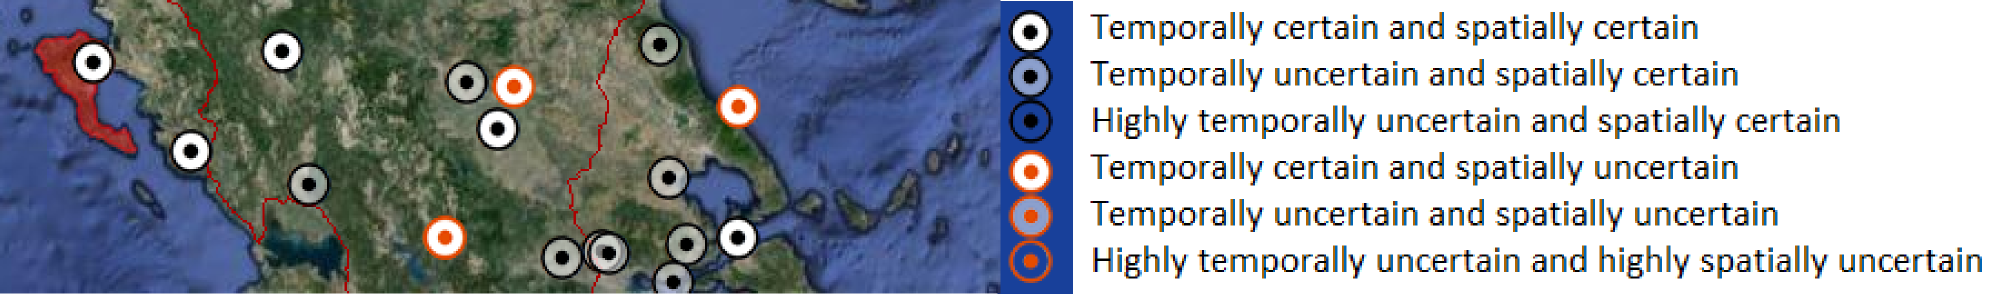
\includegraphics[width=1\textwidth]{jewish.png}
	\caption{Extrait du SIG \emph{Mapping Jewish Communities} \citep{SIGJUIFS} et l�gende associ�e.
Les lieux de peuplement des communaut�s juives de l'empire Bizantin sont symbolis�s en fonction des incertitudes associ�es � leurs composantes s�mantiques, spatiales et temporelles.}
	\label{fig:comm_juifs}
\end{figure} 


\myparagraph{Gestion des dynamiques spatiales}
La repr�sentation, visuelle ou bien dans le mod�le de donn�es, des dynamiques de l'espace constitue un besoin crucial des historiens travaillant sur des probl�mes spatialis�es.
Il para�t donc naturel que les SIG historiques fournissent des outils permettant une telle repr�sentation.
Cependant, force est constater qu'aucun syst�matisme n'existe sur les m�thodes de repr�sentation ou le niveau de consid�rations pour ces dynamiques.
\subparagraph{}
La plupart du temps, les SIG historiques se construisent autour de mod�les spatiaux et temporels (voir le paragraphe \ref{paragraph:space_as_tool}) dans lequel chaque donn�e -carte, couche vecteur, etc.- est associ�e � une date.
Cette m�thode d'association est nomm�e \emph{date stamping} \citep{Gregory2007}, et, si elle constitue un moyen simple et efficace pour situer temporellement des donn�e historiques, elle ne permet pas de mod�liser une connaissance sur leurs �volutions.
Souvent, cette repr�sentation est associ�e � des curseurs permettant de naviguer sur la ligne du temps, les donn�es correspondant � la date s�lectionn�e s'affichant alors.
La repr�sentation des dynamiques de l'espace est donc implicite et doit �tre recompos�e mentalement par l'utilisateur en \emph{d�roulant le temps}.
C'est cette repr�sentation qui se trouve au coeur de nombreux SIG historiques \citep{MAPPINGDECLINE, HISTOCOUNTIES,SIGJUIFS, SPATIALHISTO, GAPVIS, HISTOATLAS} ou encore l'outil TimeMap \citep{TIMEMAP2005}.
\subparagraph{}
Quelques SIG historiques ont d�velopp� un mod�le de donn�es visant � repr�senter les dynamiques de donn�es spatiales.
Le SIG \emph{China GIS} \citep{CHGIS} en particulier d�veloppe un mod�le de donn�es se fondant sur la repr�sentation des filiations entre zones administratives existantes � diff�rentes �poques.
Repr�sent�es par des surfaces vectoris�es, chaque unit� administrative peut �tre associ�e � des successeurs dans le temps par des liens de filiations d�crivant le type de transformations.
Ainsi, une unit� administrative existant � un temps $t=1$ donn� correspondant � l'emprise spatiale de trois unit�s administratives � $t=2$ cr�era une relation de scission, la premi�re unit� ayant �t� s�par� en deux plus petites (voir la figure \ref{fig:lineage}).
\subparagraph{}
Enfin, certains SIG historiques, �galement ax�s sur les transformations de zones administratives, mod�lisent les transformations de l'espace en d�crivant les modifications des fronti�res.
Les fronti�res, g�n�ralement consid�r�es � partir d'une p�riode initiale, sont dans un premier temps repr�sent�es et associ�es � une tranche temporelle.
Lorsqu'une modification affecte une fronti�re, celle ci est d�coup�e en plusieurs parties.
Les parts ne changeant pas voient leur p�riode temporelle agrandie, tandis que les parties modifi�es donnent naissance � de nouvelles fronti�res.
Finalement, les fronti�res deviennent un amalgame d'\emph{atomes} spatio-temporels, qui sont associ�s � chaque date pour former des fronti�res compl�tes.
Les SIG \emph{Historical Counties} \citep{HISTOCOUNTIES} et \emph{China GIS} \citep{CHGIS} mettent notamment en place de telles architectures.
\subparagraph{}
Notons d�s � pr�sent que ces mod�les constituent des instanciations, dans un cadre historique, de mod�les de donn�es spatio-temporels existants dans la litt�rature.
Ces diff�rents mod�les seront abord�s en d�tails dans le chapitre 3.

\begin{figure}[ht]
	\centering
		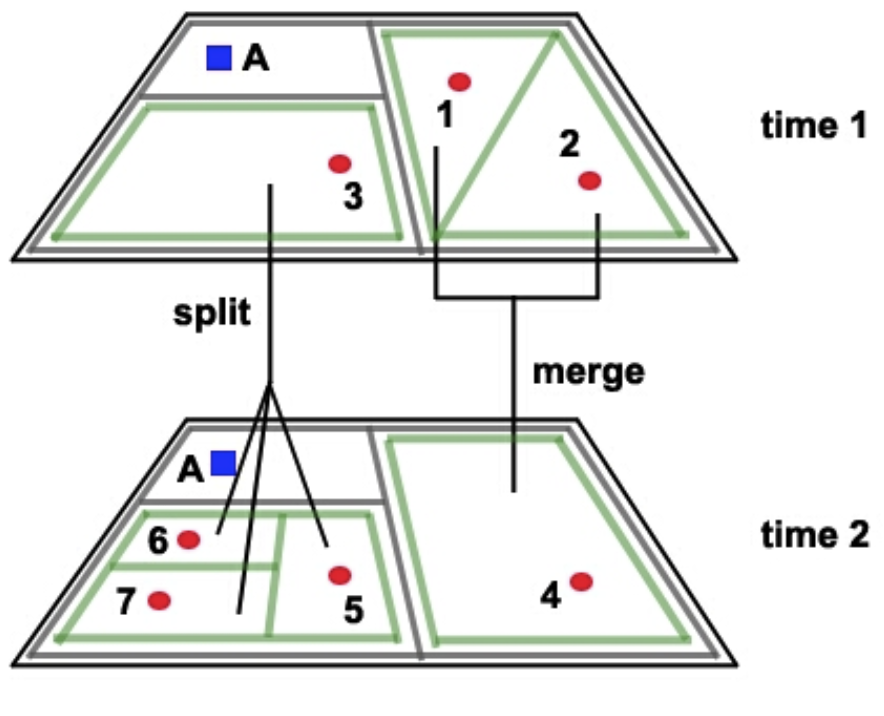
\includegraphics[width=0.4\textwidth]{chgis.png}
	\caption{Liens de filiations entre unit�s administratives dans le SIG \emph{China GIS} \cite{CHGIS}. Issue de \cite{Berman2013}.}
	\label{fig:lineage}
\end{figure} 


\myparagraph{Int�gration de donn�es historiques}
Au del� de la diffusion de donn�es historiques, les historiens voient dans les SIG un moyen de partage d'informations.
Afin de mettre en place des syst�mes ouverts et �volutifs, il est donc important de pr�voir des m�thodes permettant d'ajouter de nouvelles donn�es.
Puisque le passage entre les sources de donn�es historiques et les bases de donn�es g�ographiques n�cessitent de nombreuses op�rations, la cr�ation de m�thodes permettant d'int�grer de nouvelles informations peut devenir complexe.
Nous entendons ici le terme \emph{int�grations de donn�es} au sens de \cite{Li2011}, c'est � dire la combinaison de deux ou plus sources d'informations permettant d'obtenir une informations impossible � acqu�rir avec une source seule.
Ici, l'int�gration de donn�es concerne deux �l�ments~:
\begin{enumerate}
\item la mise en relation de donn�es spatiales implicites de fa�on � leur attribuer une localisation dans l'espace;
\item la combinaison de donn�es spatiales et d'informations sur ses transformations de fa�on � cr�er des donn�es spatio-temporelles.
\end{enumerate}
\subparagraph{}
Le premier aspect de l'int�gration s'illustre notamment au travers de GAPVIS \citep{GAPVIS}, dont l'objectif est de cartographier les r�cits contenus dans des livres anciens (antiquit� romaine en particulier).
Ainsi, � partir de textes anciens, les noms de lieux et les relations entre lieux sont extraits de fa�on automatique, puis associ�s � une localisation dans l'espace gr�ce � l'index g�ographiques en ligne Pl�iades.
De m�me, la plateforme \emph{Mapping London's Past} \citep{LONDONPAST} poss�de un outil permettant de g�ocoder automatiquement des noms de lieux dans Londres ainsi que des outils de post-traitement manuel et de v�rification des donn�es g�ocod�es.
Notons �galement que le SIG historique de Grande Bretagne subit actuellement un profond remaniement de son mod�le, s'int�ressant notamment � l'int�gration d'informations qualitatives portant sur des lieux d�crits au sein de textes \citep{Southall2012}.

\subparagraph{}
\subparagraph{}
\begin{wrapfigure}{r}{80mm}
	\centering
		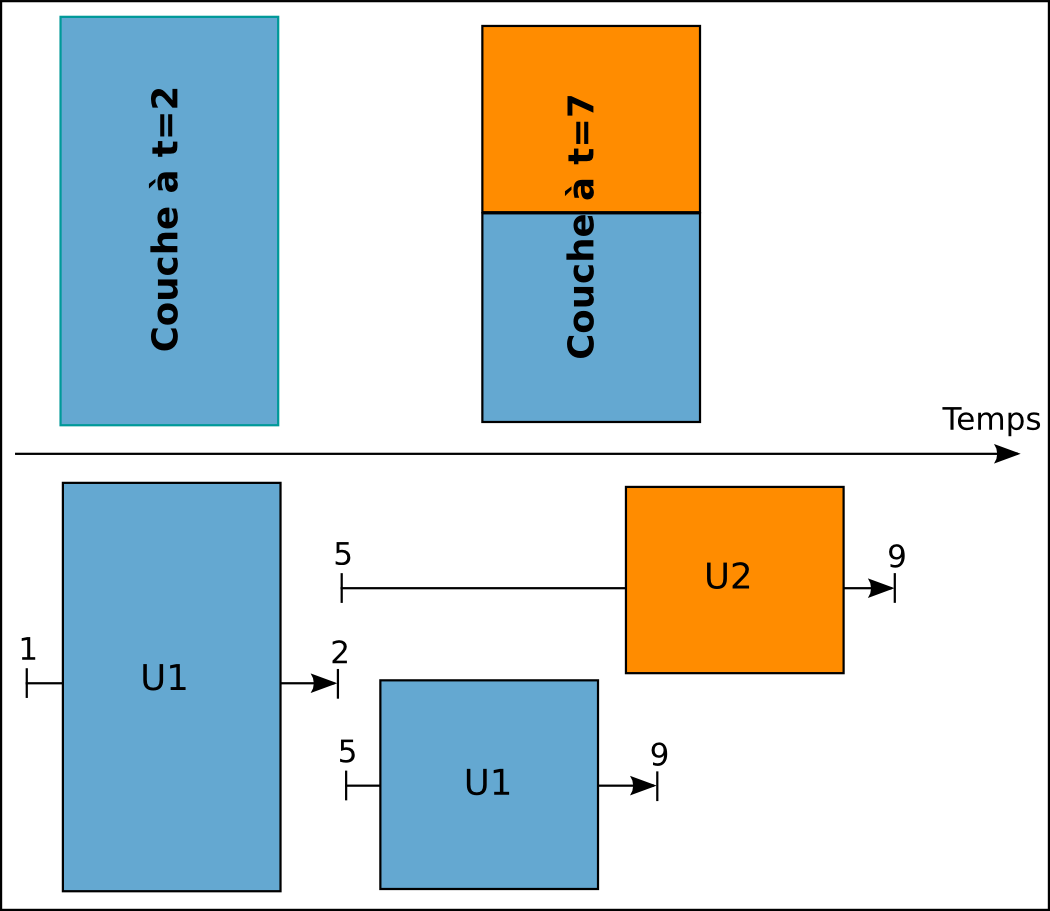
\includegraphics[width=0.35\textwidth]{chgis2.png}
	\caption{Mod�le d'objets g�ohistoriques asynchrones et couches fusionn�es dans le \emph{China GIS}}
	\label{fig:frontieres}
\end{wrapfigure}
Le \emph{China GIS} illustre pour sa part le second point de l'int�gration de donn�es g�ohistoriques.
Les donn�es manipul�es par le SIG sont un ensemble de zones administratives de la Chine ancienne, repr�sent�es sous la forme de polygones � diff�rentes p�riodes historiques.
� chacune des unit�s administratives est associ� une s�mantique (son nom et ses liens hi�rarchiques) ainsi que la p�riode temporelle de son existence.
Les diff�rentes donn�es sont alors tout � fait asynchrones, chacune �tant associ�e � une p�riode propre.
Afin de permettre la repr�sentation de l'ensemble des unit�s administratives � une date choisie tout en �vitant la r�plication des donn�es, le choix � �t� fait de fusionner les donn�es au sein d'une couche unique lors d'une requ�te temporelle.
Ainsi, lorsqu'une repr�sentation � un moment donn� est demand�, le SIG agr�ge les diff�rentes unit�s administratives dont la p�riode d'existence comprend la date demand�e, tel qu'illustr� dans la figure \ref{fig:frontieres}.
Les transformations des unit�s administratives peuvent alors �tre obtenues en fusionnant plusieurs couches � des dates diff�rents.
Leur recouvrement spatial permet d'identifier les liens de filiations existants entre les diff�rentes donn�es.

Enfin, puisqu'il s'agit pour la majorit� de plateformes web, des m�thodes d'int�gration de donn�es pourraient permettre d'ouvrir le SIG vers l'ext�rieur en le transformant en SIG collaboratif.
Pourtant, nous avons constat� qu'aucun n'a fait ce choix.
L'outil TimeMap \citep{TIMEMAP2005} permet � l'utilisateur d'ajouter ses propres informations, mais il s'agit d'avantage d'un outil de cr�ation de cartes dynamiques que d'un syst�me d'information g�ographique.
Finalement, le SIG en ligne \emph{HistoAtlas} \citep{HISTOATLAS} est pour sa part enti�rement bas� sur un processus collaboratif, la plus grande part de son contenu �tant cr�� par les utilisateurs.
Ainsi, toute personne peut ajouter des objets g�ographiques (pays ville, �v�nements, etc.), les situer dans le temps, cr�er des hi�rarchies entre objets et des cartes.
Finalement, les donn�es et les cartes ainsi cr��es sont accessibles et modifiables par d'autres utilisateurs.

\myparagraph{Bilan sur les SIG historiques existants}
Nous avons �voqu� jusqu'ici les diff�rentes strat�gies adopt�es par les SIG historiques pour r�pondre aux demandes des historiens.
Dans cette �tude rapide, on peut constater que les SIG existants r�pondent � la majorit� de ces besoins, mais souvent de mani�re incompl�te.
Ainsi, la repr�sentation visuelle des incertitudes ou des dynamiques l'emporte souvent sur leur prise en compte dans le mod�le de donn�es associ� au SIG.
L'objectif premier de ces outils �tant la diffusion de donn�es ou de r�sultats d'�tudes, il n'est pas �tonnant que l'accent soit mis en priorit� sur la repr�sentation visuelle des donn�es.
De plus, les outils de webmapping existants\footnote{Tels Geoserver (\href{http://geoserver.org}{http://geoserver.org}) et Mapserver(\href{http://mapserver.org}{http://mapserver.org})} constituent des outils puissants et aboutis qui permettent aux historiens, souvent utilisateurs finaux des outils SIG, de mettre en place des plateformes web avec une relative facilit�.
Cependant, de tels outils sont inadapt�s pour la repr�sentation de donn�es imparfaites ou la mod�lisation des dynamiques de l'espace.
En cons�quence, ils ne fournissent aucun moyen de mod�liser, repr�senter ou int�grer des donn�es spatiales comportant ces deux aspects.
On peut alors penser que cette inaptitude freine largement la mise en place de SIG historiques r�pondant de mani�re compl�te aux besoins historiques.
\\
Afin d'expliciter cette constatation, nous r�sumons les diff�rents points abord�s dans le tableau \ref{table:exgis}.
Pour chaque syst�me abord� dans les paragraphes pr�c�dents, nous avons repr�sent� sa capacit� de r�ponse aux demandes des historiens.
Chaque demande est d�compos�e en quelques strat�gies adopt�es \emph{de facto} par les SIG existants.
Un violet clair signifie que le SIG ne r�pond pas au point correspondant, tandis que le violet le plus fonc� signifie que le SIG poss�de une fonctionnalit� r�pondant totalement au crit�re.
Enfin, une couleur interm�diaire est pr�sente dans le cas o� le SIG r�pond de fa�on partielle � un crit�re, la grande diversit� de ces outils emp�chant parfois un classement clair dans une cat�gorie pr�cise.
Par exemple, si le \emph{China GIS} aborde la question de l'int�gration de donn�es par la m�thode d�crite pr�c�demment, il ne propose pas de v�ritable processus d'int�gration permettant d'ajouter de nouvelles informations de fa�on automatique et donc extensibles � d'autres donn�es.


\begin{figure}[ht]
\begin{tabular}{|l|c c|c c|c c c|c c|c c c|l|}
\hline
&\multicolumn{2}{c}{\rotatebox{90}{Diffusion de donn�es~}} & \multicolumn{2}{c}{\rotatebox{90}{Visualisation}} & \multicolumn{3}{c}{\rotatebox{90}{Incertitudes}} & \multicolumn{2}{c}{\rotatebox{90}{Dynamiques}} & \multicolumn{3}{c}{\rotatebox{90}{Int�gration}} &\\
\hline
\textbf{SIG Historique}   & \rotatebox{90}{Cartes} & \rotatebox{90}{Donn�es Spatiales} & \rotatebox{90}{Carto. en ligne} & \rotatebox{90}{R�sultats de recherche} & \rotatebox{90}{Mod�le}& \rotatebox{90}{M�tamod�le} & \rotatebox{90}{Rep. visuelle} & \rotatebox{90}{Rep. visuelle} & \rotatebox{90}{Mod�le} & \rotatebox{90}{\emph{A priori}} & \rotatebox{90}{M�thode d'int�gration} & \rotatebox{90}{Collaboratif} & \rotatebox{90}{Date de publication}\\
\hline
\emph{TimeMap} &\cellcolor{violet1}{}&\cellcolor{violet1}{}&\cellcolor{violet1}{}&\cellcolor{violet1}{}&\cellcolor{violet1}{}&\cellcolor{violet1}{}&\cellcolor{violet1}{}&\cellcolor{violet3}{}&\cellcolor{violet2}{}&\cellcolor{violet1}{}&\cellcolor{violet2}{}&\cellcolor{violet2}{}& 2004\\
\hline
\emph{Mapping Decline} &\cellcolor{violet1}{}&\cellcolor{violet1}{}&\cellcolor{violet1}{}&\cellcolor{violet3}{}&\cellcolor{violet1}{}&\cellcolor{violet1}{}&\cellcolor{violet1}{}&\cellcolor{violet3}{}&\cellcolor{violet1}{}&\cellcolor{violet3}{}&\cellcolor{violet1}{}&\cellcolor{violet1}{}& 2008\\
\hline
\emph{HistoAtlas} &\cellcolor{violet1}{}&\cellcolor{violet1}{}&\cellcolor{violet3}{}&\cellcolor{violet1}{}&\cellcolor{violet1}{}&\cellcolor{violet1}{}&\cellcolor{violet1}{}&\cellcolor{violet3}{}&\cellcolor{violet1}{}&\cellcolor{violet3}{}&\cellcolor{violet2}{}&\cellcolor{violet3}{}& 2009\\
\hline
\emph{GBHGIS} &\cellcolor{violet3}{}&\cellcolor{violet3}{}&\cellcolor{violet3}{}&\cellcolor{violet1}{}&\cellcolor{violet1}{}&\cellcolor{violet1}{}&\cellcolor{violet1}{}&\cellcolor{violet1}{}&\cellcolor{violet1}{}&\cellcolor{violet3}{}&\cellcolor{violet1}{}&\cellcolor{violet1}{}& 2009\\
\hline
\emph{NHGIS} &\cellcolor{violet1}{}&\cellcolor{violet3}{}&\cellcolor{violet1}{}&\cellcolor{violet1}{}&\cellcolor{violet1}{}&\cellcolor{violet1}{}&\cellcolor{violet1}{}&\cellcolor{violet1}{}&\cellcolor{violet1}{}&\cellcolor{violet3}{}&\cellcolor{violet1}{}&\cellcolor{violet1}{}& 2010\\
\hline
\emph{CHGIS} &\cellcolor{violet1}{}&\cellcolor{violet3}{}&\cellcolor{violet1}{}&\cellcolor{violet1}{}&\cellcolor{violet2}{}&\cellcolor{violet1}{}&\cellcolor{violet1}{}&\cellcolor{violet1}{}&\cellcolor{violet3}{}&\cellcolor{violet3}{}&\cellcolor{violet2}{}&\cellcolor{violet1}{}& 2010\\
\hline
\emph{Alpage} &\cellcolor{violet3}{}&\cellcolor{violet3}{}&\cellcolor{violet3}{}&\cellcolor{violet3}{}&\cellcolor{violet1}{}&\cellcolor{violet3}{}&\cellcolor{violet1}{}&\cellcolor{violet1}{}&\cellcolor{violet1}{}&\cellcolor{violet3}{}&\cellcolor{violet1}{}&\cellcolor{violet1}{}& 2010\\
\hline
\emph{Locating London past} &\cellcolor{violet1}{}&\cellcolor{violet1}{}&\cellcolor{violet3}{}&\cellcolor{violet1}{}&\cellcolor{violet1}{}&\cellcolor{violet1}{}&\cellcolor{violet1}{}&\cellcolor{violet1}{}&\cellcolor{violet1}{}&\cellcolor{violet3}{}&\cellcolor{violet3}{}&\cellcolor{violet1}{}& 2011\\
\hline
\emph{Valley of the shadow} &\cellcolor{violet1}{}&\cellcolor{violet1}{}&\cellcolor{violet1}{}&\cellcolor{violet3}{}&\cellcolor{violet1}{}&\cellcolor{violet1}{}&\cellcolor{violet1}{}&\cellcolor{violet2}{}&\cellcolor{violet1}{}&\cellcolor{violet3}{}&\cellcolor{violet1}{}&\cellcolor{violet1}{}& 2011\\
\hline
\emph{MJCB} &\cellcolor{violet1}{}&\cellcolor{violet1}{}&\cellcolor{violet2}{}&\cellcolor{violet3}{}&\cellcolor{violet2}{}&\cellcolor{violet1}{}&\cellcolor{violet3}{}&\cellcolor{violet3}{}&\cellcolor{violet1}{}&\cellcolor{violet3}{}&\cellcolor{violet1}{}&\cellcolor{violet1}{}& 2011\\
\hline
\emph{GAPVIS} &\cellcolor{violet1}{}&\cellcolor{violet1}{}&\cellcolor{violet3}{}&\cellcolor{violet1}{}&\cellcolor{violet1}{}&\cellcolor{violet1}{}&\cellcolor{violet1}{}&\cellcolor{violet3}{}&\cellcolor{violet1}{}&\cellcolor{violet3}{}&\cellcolor{violet3}{}&\cellcolor{violet3}{}& 2011\\
\hline
\emph{Historical counties} &\cellcolor{violet1}{}&\cellcolor{violet1}{}&\cellcolor{violet3}{}&\cellcolor{violet1}{}&\cellcolor{violet1}{}&\cellcolor{violet3}{}&\cellcolor{violet1}{}&\cellcolor{violet3}{}&\cellcolor{violet2}{}&\cellcolor{violet3}{}&\cellcolor{violet2}{}&\cellcolor{violet1}{}& 2012\\
\hline
\emph{Spatial History} &\cellcolor{violet1}{}&\cellcolor{violet1}{}&\cellcolor{violet3}{}&\cellcolor{violet3}{}&\cellcolor{violet1}{}&\cellcolor{violet1}{}&\cellcolor{violet1}{}&\cellcolor{violet3}{}&\cellcolor{violet1}{}&\cellcolor{violet3}{}&\cellcolor{violet1}{}&\cellcolor{violet1}{}& 2013\\
\hline
\emph{David Rumsey Collection} &\cellcolor{violet3}{}&\cellcolor{violet1}{}&\cellcolor{violet3}{}&\cellcolor{violet1}{}&\cellcolor{violet1}{}&\cellcolor{violet1}{}&\cellcolor{violet1}{}&\cellcolor{violet1}{}&\cellcolor{violet1}{}&\cellcolor{violet3}{}&\cellcolor{violet1}{}&\cellcolor{violet1}{}& 2013\\
\hline
\emph{Geoportail} &\cellcolor{violet1}{}&\cellcolor{violet1}{}&\cellcolor{violet3}{}&\cellcolor{violet1}{}&\cellcolor{violet1}{}&\cellcolor{violet1}{}&\cellcolor{violet1}{}&\cellcolor{violet1}{}&\cellcolor{violet1}{}&\cellcolor{violet3}{}&\cellcolor{violet1}{}&\cellcolor{violet1}{}& 2013\\
\hline
\end{tabular}
\caption{Tableau r�capitulatif des fonctionnalit�s de 15 SIG historiques existants.
\colorbox{violet1}{ }~: Non prise en compte. \colorbox{violet2}{ }~: Prise en compte partielle ou traitement manuel. \colorbox{violet3}{ }~: Prise en compte totale.}
\label{table:exgis}
\end{figure}
%
%\begin{center}
%\fcolorbox{black}{white}{
%  \begin{minipage}[t]{0.9\textwidth}
%\begin{center}
% \textbf{R�sum� de la section}
%\end{center}
%Au travers de cette section, nous avons explor� diff�rentes propositions d'outils SIG historiques mis en place au cours des derni�res ann�es, choisis en raison de leur importance ou d'une fonctionnalit� originale.
%Chaque SIG a alors �t� confront� aux diff�rents besoins exprim�s par les historiens, de fa�on � faire appara�tre le niveau d'ad�quation entre ces besoins et les outils existants.
%\subparagraph{}
%Finalement, nous avons constat� que si la diffusion de donn�e historiques, le croisement de sources et le partage de r�sultats de recherche est aujourd'hui un trait majeur des SIG, il ne r�pondent que tr�s sommairement au besoin de repr�sentation et de manipulation d'espaces dynamiques.
%De plus, ils n'offrent pas la souplesse et la prudence d'usage qu'imposent des sources toujours imparfaites.
%  \end{minipage}
%} 
%\end{center}


\section{Positionnement}
\label{section:positionnement}
\myparagraph{Constatations}
Au travers des sections pr�c�dentes, nous avons vu que la reconstitution pr�cise de l'espace ancien constitue une ressource de premi�re importance dans le cadre d'un travail historique sur la ville.
Elle agit comme un pivot pour l'�tude de donn�es sociales car il permet de situer les individus, les activit�s et les �v�nements au sein d'un r�f�rentiel commun.
Mais il peut �tre �galement lui-m�me objet d'�tude lorsqu'il est consid�r� dans une relation syst�mique avec les activit�s humaines, lorsqu'il est pris comme composante d'un territoire.
Dans les deux cas, s'appuyer sur l'espace pour �tudier un ph�nom�ne social par nature dynamique impose de consid�rer un espace �galement dynamique, dont les transformations dans le temps se lient avec les activit�s humaines.
\subparagraph{}
Les syst�mes d'informations g�ographiques, par leur capacit� � manipuler ,stocker et repr�senter une information spatiale ont attir� les sciences sociales, en particulier les historiens, au cours des dix derni�res ann�es.
Pour un travail historique, les SIG sont d�s lors de puissants outils permettant de centraliser, de partager, d'analyser et de cartographier des ph�nom�nes sociaux et spatiaux s'�tait d�roul�s dans le pass�.
Ils permettent de fournir des repr�sentations visuelles, mais aussi de constituer des bases de donn�es spatiales sur les formes des espaces pass�s de grande taille.
\subparagraph{}
Lorsqu'il s'agit de la ville, la constitution de repr�sentations et de bases de donn�es globales d�pendent de nombreuses sources historiques extr�mement h�t�rog�nes.
Les cartes anciennes, en particulier les plans de villes forment le socle fondamental de la reconstitution d'un espace ancien.
Tr�s diverses, ces sources, tout comme l'information spatiale qu'elles portent sont imparfaites.
Ainsi, la fiabilit� de chaque source historique doit �tre questionn�e avant d'�tre utilis�e dans un travail historique, les informations qu'elle portent pouvant �tre incertaines, ambigu�s ou lacunaires.
\subparagraph{}
Si la prise en compte de ces imperfections fait partie int�grante de la pratique quotidienne d'un chercheur, habitu� � confronter chaque information � d'autres sources en les croisant et en analysant leur consistance, la capacit� des SIG � manipuler une telle information doit �tre questionn�e.
Au travers de l'exploration de diff�rents SIG d�di�s � l'�tude historique, nous avons clairement fait appara�tre la faible capacit� de ces syst�mes � manipuler, mod�liser et repr�senter des donn�es spatiales imparfaites.
Nous l'avons vu, la prise en compte des imperfections de l'information se limite la plupart du temps � la minimisation des d�formations des cartes g�or�f�renc�es.
Seul les SIG \emph{ALPAGE} et \emph{Historical Counties} tentent de mod�lisent l'incertitude de leurs donn�es au sein d'un sch�ma de m�tadonn�es.
Quant � la repr�sentation visuelle des incertitudes, seul le SIG \emph{Mapping Jewish Communities} \citep{SIGJUIFS} propose une symbolisation sp�cifique de l'incertitude des donn�es qu'il cartographie.
\subparagraph{}
Enfin, la mod�lisation des dynamiques de l'espace manque �galement dans la majorit� des SIG existants, malgr� l'importance de ce besoin parmi la communaut� des historiens.
En effet, bien que cette dimension apparaisse comme essentielle pour analyser les transformations connues au cours du temps par un lieu et une soci�t�, seuls les auteurs du\emph{China GIS} \citep{CHGIS} mod�lisent explicitement les transformations des donn�es spatiales qu'ils manipulent.
Dans le cas du SIG \emph{Historical Counties} et \emph{TimeMap}, les transformations des objets spatiaux ne sont pas mod�lis�es explicitement.
En effet, seules sont stock�es des dates de d�but et de fin d'existence de chaque objet, la repr�sentation des dynamiques �tant d�s lors uniquement visuelle gr�ce � la production de cartographies dynamiques.
Notons cependant que pour \emph{Historical Counties}, les changements sont tout de m�me d�crits dans les m�tadonn�es.
\subparagraph{}
Finalement, on constate au travers du tableau \ref{table:exgis} que pour la majorit� des SIG, l'int�gration des donn�es est effectu�e soit \emph{a priori}, soit de fa�on manuelle.
Plus encore, les seuls syst�mes qui poss�dent des outils d'int�gration automatique des donn�es historiques sont d�di�s � la localisation de lieux ou d'individus, c'est � dire � au g�ocodage de l'information.
Ainsi, GAPVIS s'appuie sur des index g�ographiques en ligne pour localiser des lieux anciens, tandis que le SIG \emph{Locating London Past} utilise des banques de donn�es d'adresses pour placer des individus dans l'espace.
\subparagraph{}
L'ordonnancement chronologique propos� dans le tableau \ref{table:exgis} ne fait pas appara�tre de tendances particuli�res dans l'�volution ce ces syst�mes, sinon par le d�veloppement des outils de visualisation de donn�es en ligne.
Si une consid�ration pour les imperfections des donn�es semble appara�tre � partir de la publication du \emph{China GIS}, la mod�lisation des dynamiques de transformation des objets �tudi�s est rarement trait�e, la cartographie dynamique restant l'outil d'exploration spatio-temporel privil�gi�.
Il faut cependant rester prudent~: le tri temporel est effectu� sur les derni�res versions de chacun des SIG, certaines versions anciennes peuvent pr�senter des fonctionnalit�s complexes.
C'est par exemple le cas pour \emph{Historical Countier}, dont la cr�ation des bases de donn�es spatiales a commenc�e en 1987 \footnote{http://publications.newberry.org/ahcbp/project.html}.


\myparagraph{Hypoth�ses et objectif}
Nous nous pla�ons dans le cadre de la mod�lisation de l'espace urbain ancien au sein d'un SIG historique.
Nous avons identifi� dans les sections \ref{section:SIG} et \ref{section:SIG} deux demandes importantes des historiens adress�es � de tels outils~:
\begin{itemize}
 \item La possibilit� de centraliser, croiser et diffuser des donn�es et des sources g�ohistoriques.
\item La mod�lisation des dynamiques de l'espace en vue de leur analyse.
\end{itemize}
Au travers de l'exploration des SIG historiques existants, nous avons constat� qu'ils r�pondent � l'heure actuelle de fa�on satisfaisante � la premi�re demande, notamment gr�ce aux initiatives de cr�ation de SIG en ligne de niveau national tels \emph{ China GIS, NHGIS} ou \emph{GBHGIS}.
\subparagraph{}
Le deuxi�me point cependant fait cruellement d�faut au sein des outils et syst�mes existants � l'heure actuelle.
S'il est commun�ment admis \citep{Gregory2007, Knowles2008} que ce manque est principalement d� � l'incapacit� des outils grand publique � manipuler des donn�es imparfaites et spatio-temporelles, force est de constater que le d�veloppement des syst�mes plus sp�cialis�s n'a pas abouti � la proposition d'outils ou de mod�les adapt�s aux besoins de l'histoire.
En effet, les SIG historiques restent aujourd'hui d�di�s � des applications sp�cifiques et ne sont pas destin�s � �tre utilis�s comme outils dans d'autres �tudes historiques.

\subparagraph{}
On peut alors penser que l'absence d'un mod�le r�pondant au second besoin des historiens provient d'un manque de m�thodes d�di�es � la constitution de bases de donn�es spatio-temporelles � partir de donn�es g�ohistoriques issues de sources h�t�rog�nes.
En effet, nous avons vu que dans la majorit� des cas, les donn�es spatio-temporelles sont cr�es de fa�on manuelle � partir de diverses sources, qu'elles aient �t� saisies en amont de la construction du SIG ou ajout�es au fur et � mesure.
Tout comme l'indique \cite{Arnaud2008}, la recomposition des dynamiques spatiales � partir uniquement de sources historiques agissant comme des \emph{tranches temporelles} est une t�che fastidieuse dont la complexit� est extr�me lorsque les sources sont imparfaites.
\subparagraph{}
La mise en place d'un processus d'int�gration de donn�es g�ohistoriques visant � constituer des donn�es spatio-temporelles peut permettre d'augmenter la g�n�ricit� d'un SIG historique. L'automatisation de ce processus est donc un atout important.
Cependant, nous pensons que la complexit� des sources g�ohistoriques ainsi que les connaissances mise � l'\oe uvre pour comprendre, analyser et critiquer une source rendent peu pertinent la mise en place de processus d'int�gration enti�rement automatis�s.
\subparagraph{}
Comme nous l'avons vu dans la section \ref{section:usages}, la reconstruction d'un espace ancien permet de produire des donn�es g�ohistoriques � la fois spatiales et temporelles.
Afin d'obtenir une repr�sentation des dynamiques de cet espace, il est n�cessaire d'op�rer la mise en relation des diff�rents objets porteurs d'informations spatiales pour des temporalit�s diff�rentes pour constituer des bases de donn�es g�ohistoriques de nature proprement spatio-temporelles.
Une fois ces donn�es constitu�es, leurs transformations peuvent �tre analys�es.
\subparagraph{}
Nous avons �galement soulign� en section \ref{subsection:plans} l'importance des plans lorsqu'il s'agit d'�tudier un espace ancien.
Dans le cas des villes plus particuli�rement, et pour des p�riodes r�centes, ces sources fournissent la partie la plus significative des informations sur leurs structures et leur organisation. En nous fondant sur ce constat, nous avons donc choisi de concentrer notre travail sur le traitement des informations spatiales issues de plans de villes anciens.
Plus pr�cis�ment, dans le cadre de cette th�se, l'espace consid�r� sera la ville de Paris entre les XVIII\up{e} et XX\up{e} si�cles, en raison de la richesse des ressources cartographiques d�crivant la ville, mais �galement de l'intensit� des transformations qu'elle conna�t en l'espace de deux si�cles (voir le chapitre 2).
\subparagraph{}
En r�sumant, dans notre travail nous nous sommes fix� trois objectifs principaux~:
\textbf{
\begin{itemize}
 \item Constituer une base de donn�es spatiale et temporelle de donn�es vectorielles extraites de plans de villes anciens.
\vspace{11pt}
 \item Proposer aux historiens une m�thode semi-automatique pour la constitution de bases de donn�es spatio-temporelle, � partir de l'analyse, du traitement et de la mise en relation de sources historiques � contenu spatial.
\vspace{11pt}
 \item Mod�liser et de prendre en compte, au sein des diff�rentes �tapes de l'int�gration des donn�es g�ohistoriques, les diff�rentes imperfections qui entachent l'information manipul�e.
\end{itemize}
}
\newpage
\section{Conclusion}
Dans ce chapitre, nous avons tout d'abord identifi� les principales fonctionnalit�s qu'un SIG historique doit poss�der pour �tre adapt� aux besoins des chercheurs en histoire. Pour cela, nous avons explor� comment l'espace g�ographique �tant actuellement utilis� dans diff�rents travaux de recherche en histoire urbaine. Nous avons vu la n�cessit� de visualiser, analyser et manipuler les dynamiques de transformation des objets g�ographiques urbains. En effet, les ph�nom�nes sociaux �tudi�s �voluent conjointement � l'espace dans lequel ils se d�roulent. Ils interagissent �galement avec lui, rendant ainsi leur analyse compl�te seulement possible si l'espace est consid�r� dynamique. Sur ce point, nous avons list� les principaux SIG historiques existants et constat� qu'ils ne r�pondent pas � ce besoin. Ceux-ci sont en r�alit� statiques, peu extensibles et servent principalement de plateforme de diffusion de donn�es brutes et de r�sultats de travaux. Ils ne fournissement en g�n�ral pas d'outils d'analyse de ces donn�es et ne permettent pas de manipuler et d'analyser des objets g�ographiques en transformation dans le temps.
Ces manques sont notamment dus aux complexit�s des sources historiques, imparfaites et difficiles � int�grer car demandant d'importants traitements (num�risation, vectorisation, etc.). 
\\
De cette �tude, nous avons d�gag� l'objectif principal de cette th�se~: mettre en place une approche permettant de constituer des bases de donn�es spatio-temporelles d�crivant les transformations de l'espace urbain � partir de sources cartographiques anciennes.
\\
Notre cas d'application est la ville de Paris aux XVIII et XIX\textsuperscript{e} si�cles. Nous avons point� dans ce chapitre la n�cessit� d'une connaissance fine des  sources utilis�es si l'on veut utiliser sans risque d'erreurs les informations qu'elles contiennent. Nous proc�dons � cette analyse dans le prochain chapitre sur cinq sources cartographiques parisiennes que nous utiliserons pour exp�rimenter et valider l'approche propos�e au long de ce travail.
 % Positionnement du sujet : positionnement par rapport � la pratique de l'histoire et aussi par rapport � l'utilisation de SIG pour faire de l'histoire.
\chapter{Sources cartographiques sur Paris}
\label{chap:sources}

\renewcommand{\labelitemi}{\tiny$\blacksquare$}
\large \begin{mybox} \normalsize
\textbf{Objectifs~:} 
\vspace{11pt}
\begin{itemize}
\item  Pr�senter les sources topographiques parisiennes utilis�es.
\vspace{11pt}
\item  Identifier les h�t�rog�n�it�s des sources et les liens d'h�ritages existants entre elles.
\vspace{11pt}
\item  D�terminer de fa�on qualitative les temporalit�s valides des sources.
\vspace{11pt}
\item  Explorer la mutation de d'administration de la Seine � travers les plans de Paris.
\end{itemize}
\end{mybox}
\renewcommand\labelitemi{\textbullet}% bullet
\newpage
\minitoc
\newpage
Traiter des plans anciens au sein d'un SIG implique n�cessairement qu'ils soient proches des plans topographiques contemporains pour lesquels ont �t� d�velopp�s les outils et les m�thodes de traitement actuels. Cette proximit� est tout d'abord cartographique~: la vue doit �tre verticale, les th�mes cartographiques semblables. Elle doit �tre aussi g�om�trique, dans la pr�cision du positionnement des objets dans le plan de la carte~: il faut donc des plans marqu�s par une forte pr�cision, pr�sentant de faibles d�formations g�om�triques. Les plans en perspective, majoritaires avant le XVIII\up{e} si�cle, sont donc difficilement utilisables par un SIG � deux dimensions \footnote{On parle de SIG 2D pour d�signer les outils classiques destin�s � la cartographie, en opposition aux SIG 3D qui permettent de repr�senter des donn�es g�ographiques en volume.}
\cite{Balletti2000}, ayant r�f�renc� un plan de la ville de Venise en pla�ant un ensemble de points d'amer sur des b�timents dessin�s en perspective, a conclu � une difficult� de comparaison du r�sultat avec des donn�es planim�triques, et ce, malgr� un g�or�f�rencement satisfaisant.
Plus g�n�ralement, de telles vues sont davantage utilis�es dans le cadre de SIG � trois dimensions ou pour la reconstitution d'�difices anciens en arch�ologie~\citep{Stefani2010}.
C'est par exemple le cas du \emph{Virtual Lodeum}~\citep{Pfeiffer2013}, SIG 3D de la ville de Li�ge constitu� � partir d'une maquette de 1730, dans lequel des gravures anciennes de b�timents peuvent �tre projet�es sur les mod�les 3D correspondants.
\subparagraph{}
Les transformations les plus importantes de l'espace parisien que l'on peut ais�ment documenter se situent durant les XVIII\up{e}, XIX\up{e} et XX\up{e} si�cles.

La population parisienne passe ainsi d'environ 640.000 �mes en 1793~\citep{Landry1935} � 600.000 en 1811, d�passe le million en 1846 pour atteindre 1.200.000 en 1856~\citep{Chevalier1952} dans les m�mes limites.
En 1891 la ville compte plus de 2.440.000 habitants, soit pr�s de quatre fois la population cent ans plus t�t.
La ville se transforme en profondeur et � plusieurs reprises~: la R�volution am�ne la vente des anciennes propri�t�s eccl�siastiques et lib�re de larges espaces lotissables, tandis que le Consulat et le Premier Empire mettent en place des politiques de grand travaux~: canal de l'Ourcq et r�servoirs, abattoirs, quais, etc. Aux grandes op�rations de lotissement de Grenelle et Plaisance au sud, Passy � l'ouest ou encore Poissonni�re et Batignolles au nord succ�dent les premi�res grandes perc�es~: la poursuite de la rue de Rivoli au travers du centre parisien ou la rue Rambuteau sont ouvertes.
Au milieu du XIX\up{e} si�cle c'est le centre parisien qui subit les politiques hygi�nistes des autorit�s centrales; les rues sont �largies, rendues rectilignes, les impasses deviennent des rues.
Surviennent ensuite le rattachement des communes limitrophes qui agrandit Paris de  4.365 hectares, puis les op�rations haussmanniennes qui poursuivent la transformation de la ville.
Apr�s 1885, Paris ne conna�tra plus de transformations majeures, sinon dans le quartier de la Villette en raison du d�veloppement des industries~\citep{Bourillon2000}.
\subparagraph{}
Dans ce cadre, nous avons choisi de nous concentrer sur la p�riode allant de la R�volution Fran�aise � la fin du XIX\up{e} si�cle.
Ainsi, nous couvrons une p�riode marqu�e par des modifications majeures mais aussi par une riche production de plans topographiques.
En effet, la rapidit� des transformations urbaine s'accompagne d'une profusion de plans souvent r�alis�s par des architectes.
\subparagraph{}
Simples guides de la ville, la plupart de ces plans sont � une �chelle trop grande et sont trop peu pr�cis pour �tre utilisables comme sources principales d'information sur l'espace parisien.
Certains d'entre eux se distinguent cependant par une tr�s grande pr�cision et une �chelle fine, entre 1/2.000\up{e} et 1/10.000\up{e}.
Ils sont pour la plupart li�s aux instances du pouvoir parisien et ils �taient destin�s � �tre de v�ritables outils d'am�nagement de la ville, ce qui permet de les consid�rer comme les sources les plus pr�cises et fiables sur la topographie de Paris.
Ainsi, nous avons s�lectionn�s cinq plans qui nous permettent de couvrir la totalit� de la p�riode consid�r�e~:
\begin{itemize}
\item l'\emph{Atlas National de la ville de Paris} par Edm� Verniquet, publi� entre 1791 et 1799. On le d�signera par souci de simplicit� \emph{atlas de Verniquet},
\item la \emph{Topographie de Paris}, plan r�alis� par Nicolas Maire et publi� en 1808. Il sera nomm� \emph{plan de Maire},
\item le \emph{cadastre de Paris par �lots} de Philibert Vasserot, commenc� en 1810 et termin� en 1836 (1855 pour certains �lots). On l'appellera \emph{Cadastre de Vasserot},
\item l'\emph{Atlas G�n�ral de la ville et des faubourgs de Paris} de Th�odore Jacoubet, publi� en 1836. Il sera nomm� \emph{atlas de Jacoubet},
\item l'\emph{Atlas municipal des vingt arrondissements de la ville de Paris}, plan officiel de la pr�fecture de la Seine, �dition de 1888. Il sera d�sign� comme un \emph{atlas municipal}.
\end{itemize} 
Parmi ces plans, seul le dernier est officiellement issu des services municipaux, tous les autres �tant le produit d'entreprises individuelles\footnote{Si le projet est � l'initiative d'une seule personne -architecte, commissaire voyer, etc.-, des �quipes de taille vari�e travaillerons � la r�alisation de chaque plan. Plus de 40 g�om�tres participerons par exemple � la r�alisation de l'atlas de Verniquet.}. Nous verrons au cours de ce chapitre qu'il s'agit bien d'une caract�ristique propre de cette p�riode qui marque la nature de ces sources aussi bien du point de vue technique que de leur utilisation dans le cadre de la politique urbaine de Paris. Issus d'un travail individuel, ces plans �taient lev�s sur des p�riodes souvent longues. Ils �taient aussi objets d'un march� de vente, �change, reprise et diffusion qui impactait non seulement les formes des uns sur les autres mais induisant aussi la reproduction non contr�l�e de leurs erreurs et impr�cisions. Dans plusieurs cas, une analyse attentive, permet en effet de voir comment, dans une m�me planche, architectes et g�om�tres r�utilisaient des lev�s ou des repr�sentations cartographiques ant�rieures, conservant alors leurs erreurs et impr�cisions. Si ces aspects sont connus des historiens, ils ont �t� rarement consid�r�s dans la construction des SIG historiques existants qui acceptent de les int�grer sans un v�ritable travail critique. Au cours de ce chapitre, nous essayerons donc d'analyser qualitativement le contexte, la structure et le contenu de chaque plan, de fa�on � d�terminer plus pr�cis�ment leur nature, notamment en ce qui concerne les temps de validit�, aspect qui est tr�s souvent difficile de d�terminer, comme nous avons vu au cours du chapitre pr�c�dent. 

Une telle d�marche s'est r�v�l�e particuli�rement fructueuse.  Ainsi nous avons pu d�montrer que, pour l'ensemble de ces plans, les dates officielles de publication ne refl�tent jamais la r�alit� de terrain des planches qui les composent. Emprunts, reprises, nouveaux lev�s et projets d'ouverture se superposent de mani�re souvent contradictoire en restituant surtout l'image d'un plan comme d'un millefeuille qui accumule les fragments locaux d'une ville qui change sans cesse. La complexit� de ce tramage temporel est donc avant tout le r�sultat  presque in�vitable induit par les techniques de travail de l'�poque. Mais nous avons pu voir qu'elle r�v�le aussi une dynamique plus complexe donn�e par le changement des formes de production de l'objet cartographique qui passent de la dimension de l'entreprise priv�e � celle du public. Si Edm� Verniquet avait travaill� sur son plan en tant que g�om�tre priv� commissionn� par l'administration pr�fectorale, Th�odore Jacoubet produira le sien en tant que fonctionnaire du Bureau des Plans de la ville de Paris.  Dans les plans lev�s au cours du XIX�me si�cle, nous trouvons donc aussi la trace de nombreuses tensions qui marquent ce processus. Tout au long du si�cle les int�r�ts priv�s et int�r�ts publics se superposent de mani�re souvent contradictoire en impactant tr�s souvent sur la qualit� et m�me la v�racit� des lev�s. Au centre de cette p�riode et de ces changements, l'analyse de la figure de Th�odore Jacoubet et de son travail permet de mesurer tr�s pr�cis�ment la nature et l'importance de ces d�terminations.

\section{Atlas de Verniquet}
\label{subsection:verniquet}
L'\emph{Atlas National de la Ville de Paris}\footnote{Le nom complet de cet atlas est \emph{Atlas du Plan G�n�ral de la Ville de Paris, lev� g�om�triquement par le citoyen Verniquet, rapport� sur une �chelle d'une demi ligne pour toise et divis� en 72 planches.}} est � la fois l'{\oe}uvre majeure de son auteur, l'architecte Edm� Verniquet, et la matrice de la plupart des plans parisiens du XIX\up{e} si�cle.
Termin� en 1791, cet atlas compos� de 72 feuilles � l'�chelle de 1/1.800 environ (� l'origine, le plan est en toises � une �chelle d'une demi-ligne par toise) est un portrait de la ville � l'aube de la R�volution.
La pr�cision extr�me du plan et le style d�pouill� qui lui sont caract�ristiques feront de lui la base de la plupart des grands plans de Paris pendant de nombreuses ann�es et un outil convoit� par l'administration de la Seine.
Ce n'est pourtant ni le plan le plus riche d'informations, ni le plus novateur de son �poque.
En 1730 d�j� des cartographes tel Delagrive s'�taient attach�s � concevoir des plans de Paris dits \emph{g�om�traux} o� la pr�cision g�om�trique �tait l'objectif principal.
On conna�t aujourd'hui l'ampleur et les d�tails de la t�che de Verniquet gr�ce aux travaux de Jeanne Pronteau~\citep{Pronteau1986} qui a reconstitu� toutes les �tapes de la construction du plan, depuis l'achat du titre de commissaire-voyer par Verniquet\footnote{Verniquet prend en effet la suite de Turgot en 1774 apr�s avoir achet� son titre de commissaire voyer � la ville de Paris pour 100.000 livres.} jusqu'aux derni�res gravures des feuilles du plan en 1799.
Bien qu'il s'agisse du plus ancien plan que nous utilisons, ces travaux nous offrent la possibilit� de conna�tre en d�tail la phase, pour nous cruciale, du lev� du plan.
Il s'agira d'ailleurs de l'unique plan pour lequel nous connaissons avec pr�cision la p�riode de lev�.

\subsection{Lev� et structure}
Jeanne Pronteau d�crit pr�cis�ment toutes les op�rations qui ont men� � la construction de l'atlas de Verniquet. Nous n'en ferons ici qu'une synth�se rapide et certainement incompl�te, mais dont l'objectif est de faire appara�tre les diff�rentes couches temporelles qui constituent l'atlas final.
\subparagraph{}
La premi�re chose � noter est que la grande majorit� des lev�s topographiques effectu�e par Verniquet ne concernent pas la construction du fameux atlas. Son objectif est, � l'origine, la constitution d'un plan de Paris rue par rue. C'est dans ce but qu'il entame en 1775 le relev� topographique de l'ensemble des rues de Paris, dans un premier temps � ses frais, puis, � partir de 1783, officiellement charg� par l'administration royale\footnote{Jeanne Pronteau indique ainsi que de 1775 � l'�t� 1783, Verniquet proc�de � des relev�s qui deviendront officiels � la suite de la d�claration royale du 10 avril 1783.
Celle-ci fixe des r�gles entre la largeur de la rue et la hauteur des constructions qui l'entourent.
Le Roi charge alors les commissaires voyers, dont Verniquet fait partie, d'effectuer un lev� complet des rues de la ville \citep[p.409]{Pronteau1986}.}
Verniquet termine ses plans de rues en 1785 au 1/144\up{e} pour l'ensemble des rues contenues dans les limites de Paris fix�es par Louis XV\footnote{D�claration du 18 juillet 1724}.
Notons que ces plans, bien plus d�taill�s que l'atlas, contiennent, en plus de la forme des rues, les amorces des parcelles, le num�ro ainsi que le nom du propri�taire du moment.
\paragraph{}
La m�me ann�e, Verniquet demande et obtient de la part du Roi la construction d'un grand plan de Paris, qui aboutira � l'atlas que l'on conna�t aujourd'hui.
Apr�s avoir effectu� les relev�s des rues allant jusqu'� l'enceinte des Fermiers G�n�raux (Jeanne Pronteau donne ainsi 184 rues nouvellement lev�es jusqu'en 1788~\citep{Pronteau1986}) et d�sormais assist� par plus de 40 personnes, Verniquet commence � former son plan g�n�ral.
Pour cela, il r�utilise les lev�s des rues de Paris qui lui fournissent les mesures des rues puis replace par triangulation ces diff�rentes mesures dans la ville.
Finalement, il assemble toutes les rues les unes apr�s les autres pour former la structure compl�te du plan. Le plan complet de la ville de Paris est ainsi achev� en 1791, mais sa gravure s'�talera jusqu'en 1799.

\myparagraph{Structure du plan}
L'atlas de Verniquet a �t� enti�rement construit sur la base de relev�s topographiques et trigonom�triques.
� partir de la m�ridienne de Paris et de sa perpendiculaire se croisant � l'observatoire, Verniquet a effectu� une triangulation couvrant toute la ville et permettant d'assembler et de corriger les diff�rents lev�s des rues.
Cette triangulation et la structure compl�te du plan sont aujourd'hui connus non seulement par les travaux pr�c�demment cit�s, mais aussi gr�ce � un plan fourni par Verniquet � la page 70 de son Atlas.
Fourni en annexe~\ref{annexe:triangulations_verniquet}, il s'agit d'un plan r�sumant l'ensemble des points fixes choisis comme rep�re (nomm�s \emph{points de station}) et les triangles les reliant. 
Il d�finit ainsi 67 points de station dont 8 points principaux et 59 points secondaires fix�s sur des monuments remarquables (clochers, colonnes, coupoles, etc.).
Il rajoute enfin 27 points de station aux alentours de Paris, pour am�liorer � la fois les v�rifications des calculs et la pr�cision des trac�s dans les faubourgs.
Les 8 points de station principaux sont fournis avec un plan d�taill� qui permet de les placer tr�s pr�cis�ment encore aujourd'hui.
Quant aux autres points, si les 59 stations secondaires peuvent encore �tre retrouv�es car plac�es sur des �l�ments b�tis (souvent les fl�ches ou tours d'�glises, de couvents et d'autres b�timents d'importance), la plupart des 27 points des faubourgs ne peuvent pas �tre plac�s avec pr�cision (l'un d'eux indique par exemple seulement \emph{Dans la plaine de Grenelle}).
Finalement, le plan entier de Verniquet est d�coup� en 72 feuilles selon un carroyage fix� sur la m�ridienne et sa perpendiculaire.

\subsection{Contenu du plan}
L'atlas de Verniquet est en rupture avec les plans de Paris qui le pr�c�dent dans lesquels le dessin des b�timents, des cours ou des �lots est souvent tr�s d�taill�, tel celui de Jaillot.
Son {\oe}uvre est � l'inverse extr�mement �pur�e~: seuls les contours des �lots urbains sont dessin�s d'un trait d'encre, l'int�rieur �tant laiss� vide. Seul le dessin du relief, c'est notamment le cas de Montmartre, est riche en d�tails sans doute plus d�coratifs qu'indiquant la v�ritable d�nivellation. 
\paragraph{}
Certains b�timents sont cependant trac�s � l'encre et de fa�on d�taill�e.
Il s'agit en fait de l'ensemble des biens nationaux, qui seront ajout�s par Verniquet pour r�pondre � la demande de la Convention en 1793 de produire des plans de l'ensemble de ces biens dans le but de les lotir et les vendre \citep{Pronteau1986}.
Cette demande finale aboutira � la gravure, unique, de l'atlas complet entre 1793 et 1799.

\section{Plan de Maire}
Comme nous l'avons �voqu�, Paris conna�t d'importantes transformations pendant le r�gne de Napol�on I\up{e} tant en raison des politiques publiques d'urbanisme (d�molition du Grand Ch�telet, percement de la rue de Rivoli et du canal de l'Ourq, construction d'abattoirs) que des op�rations priv�es de lotissement dans les espaces des diff�rents biens nationaux qui pars�ment le centre de la ville.
\paragraph{}
Le \emph{Plan de la ville de Paris}  (ou \emph{La topographie de la Ville de Paris et de ses faubourgs}) dessin� par Nicolas Maire en 1808 est un t�moin privil�gi� des modifications apport�es par le Premier Empire, non seulement sur le tissu urbain mais aussi sur les d�nominations des rues (on remarque plus de 66 nouveaux noms de rues, auxquelles il faut ajouter les tr�s nombreuses rues ayant repris le nom qu'elles avaient avant la R�volution).
Divis� en 20 planches plus une planche d'assemblage, le plan est accompagn� par un tableau des rues et une notice explicative de l'auteur qui le pr�sente comme une version corrig�e et mise � jour du plan de Delagrive\footnote{Pr�curseur du plan de Verniquet, le plan de De La Grive a �t� publi� en 1728 puis r��dit� plusieurs fois au cours du XVIIIe si�cle, jusqu'en 1761}.
L'�chelle n'est pas not�e sur le plan, mais Maire indique qu'elle est la m�me que celle du plan de Delagrive, soit environ 1/4.500\up{�me}\footnote{Le plan de Delagrive dat� de 1728 est grav� � 11mm pour 25 toises, soit environ 1/4.429\up{�me}.
Jean Boutier~\citep{Boutier2007} aboutit �galement � une �chelle de 1/4.500\up{e}, soit 17,2 cm pour 400 toises.}, faisant de ce plan l'un des plus d�taill�s sur les ann�es 1800-1810.
\`A titre de comparaison, une autre s�rie de plans de Paris de haute qualit� �dit�s par Charles Piquet � partir de 1804 ne sont qu'� l'�chelle de 1/8.000\up{e}.
\paragraph{}
Nous ne connaissons pas pr�cis�ment les dates de r�alisation de ce plan, 1808 �tant seulement sa date de parution.
Cependant, il ne s'agit pas d'une �dition originale mais de la mise � jour d'un autre plan �dit� par le m�me auteur en 1803.
Maire corrigera et �ditera de nouveau son plan r�guli�rement, en 1812, 1813, 1816 et finalement 1824~\cite[p.226]{Bonnardot1851}.
Un tel rythme de gravure, au moins jusqu'en 1816, laisse penser qu'il s'agit surtout de corrections apport�es � un trac� r�alis� sans doute en 1803 ou avant.
\paragraph{}
On pourrait s'�tonner que l'auteur, pourtant \emph{ing�nieur g�ographe} reconnu\footnote{On le retrouve sous la Restauration avec le titre de \emph{g�ographe ordinaire du Roi}}, ne se soit pas plut�t appuy� sur l'atlas de Verniquet.
Il faut rappeler, cependant, que, tout en restant la r�f�rence principale pour la cartographie de la capitale, en 1803 Edm� Verniquet est engag� dans un important proc�s avec les administrations napol�oniennes et les exemplaires de son Atlas se trouvent dispers�s entre les diff�rents protagonistes. 
% En analysant plus finement le plan, nous allons pourtant observer qu'il est plus complexe que l'annonce l'auteur et en particulier qu'il n'est pas aussi �loign� du plan de Verniquet qu'on pourrait le croire.

\subsection{Structure du plan}
\myparagraph{Un plan issu de plusieurs sources}
En premier lieu il nous faut remettre en question la pr�sentation officielle du plan de Maire comme h�ritier d'un unique plan qui, rappelons-le, est �g� de pr�s de 80 ans.
C'est ce que Alain Fourquier sugg�rait d�j�  \citep{Fourquier2007} en montrant que Maire avait certainement utilis�s aussi deux autres plans.
Le premier, dit \emph{Plan de Jaillot} \citep{MAPJaillot1775}, dat� de 1775 � 1778, est proche du plan de Delagrive tant en termes de contenu que de construction~: repr�sentation des b�timents publics et religieux sans d�tailler les �lots, �chelle proche (environ 1/3600\up{e}), etc. Le second n'est autre que l'atlas de Verniquet.
\paragraph{}
Si les plans de Jaillot et de Delagrive ont pu servir � Maire pour dessiner l'int�rieur de Paris, ils ne couvrent pas les espaces externes � l'enceinte des Fermiers G�n�raux, pourtant repr�sent�e dans son plan. Or il est int�ressant de remarquer que les espaces de Monceau, Chaillot, Vaugirard et le sud de la Bi�vre, en dehors des limites du plan de 1728, �taient parfaitement renseign�s chez Verniquet.
L'utilisation de son plan par Maire est donc plus que cr�dible, d'autant plus que les deux g�om�tres sont contemporain (seuls 4 ans s�parent la fin de la gravure de l'atlas de Verniquet et la premi�re publication de Maire en 1803 et que les mises � jours de Verniquet �taient beaucoup plus r�centes.
\paragraph{}
Si l'on compare visuellement les faubourgs de la ville sur les plans de Maire et Verniquet, la ressemblance des styles appara�t imm�diatement.
La figure \ref{fig:verniquetvsmaire} donne ainsi deux exemples extraits de ces deux plans, le premier centr� sur les Buttes-Chaumont � l'Est et le second sur la Butte-Aux-Cailles.
On remarque ainsi qu'en plus d'une symbolisation tr�s proche, les m�mes d�tails sont repr�sent�s sur les deux plans.
De plus, dans l'espace des Buttes-Chaumont  les d�nivellations sont presque identiques et symbolis�es de la m�me fa�on, un tel niveau de d�tail ne se trouvant que dans l'atlas de Verniquet.
� c�t� de chaque extrait figure �galement la zone correspondante sur le plan de Delagrive, permettant de mieux juger de la proximit� entre les travaux de Verniquet et Maire. Il semble donc que le plan de Maire soit en fait compos� de deux sources, la premi�re sur le centre parisien et la seconde permettant la mise � jour des espaces fortement transform�s depuis 1728, en particulier autour de l'enceinte des Fermiers G�n�raux.
\begin{figure}
 \centering
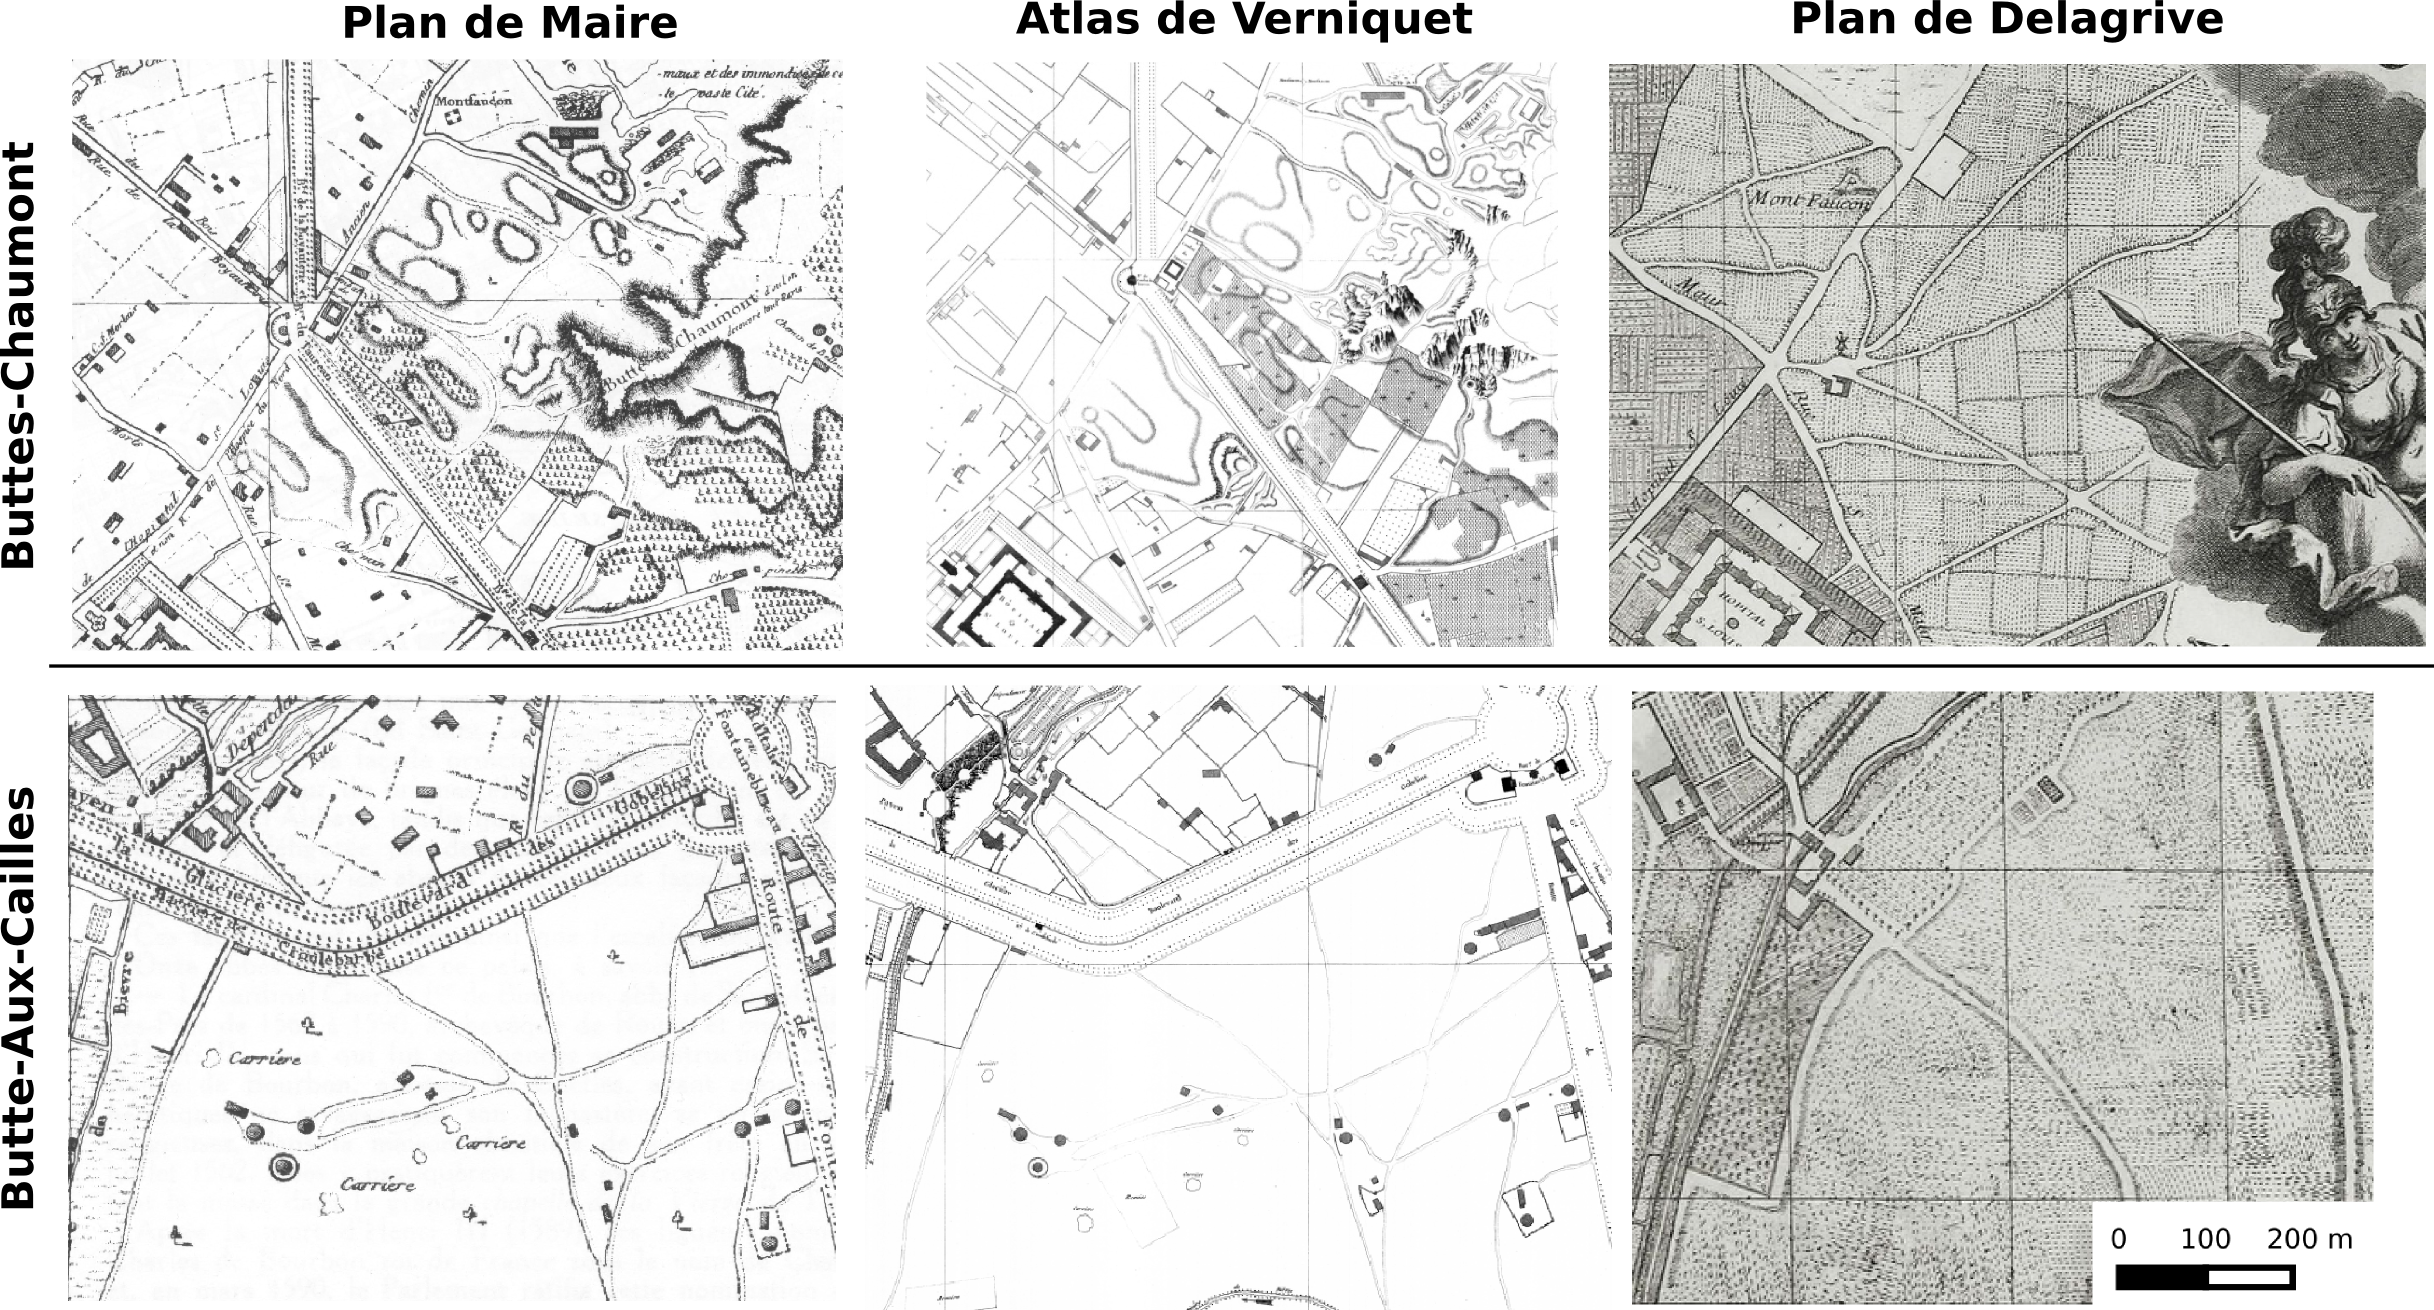
\includegraphics[width=1\textwidth]{verniquet_vs_maire.png} 
	\caption{Les Buttes-Chaumont et la Butte-Aux-Cailles telles que repr�sent�es dans le plan de Maire en comparaison avec l'atlas de Verniquet et le plan de Delagrive.}
	\label{fig:verniquetvsmaire}
\end{figure}

Le plan de Maire est donc particulier puisqu'il appara�t comme un assemblage d'au moins deux plans plus anciens et non comme une mise � jour d'un plan unique ou un nouveau lev�.
Bien que cet assemblage ait pu permettre d'obtenir un plan d�taill� pour l'ensemble de la ville en 1808, il est donc �vident qu'une telle construction peut induire une pr�cision g�om�trique h�t�rog�ne.

\myparagraph{Le carroyage du plan}
Assez �trangement, Maire ne fait pas appara�tre la m�ridienne de Paris sur son plan, et il ne construit pas non plus son carroyage � la fa�on de Delagrive et Verniquet  en utilisant la m�ridienne et sa perpendiculaire passant � l'Observatoire pour former les carreaux.
Au contraire, le carroyage, compos� de 80 rectangles de 900 m�tres sur 640 m�tres, pr�sente un d�calage de plus de 300 m�tres � l'ouest de la m�ridienne, et de pr�s de 150 m�tres au nord de sa perpendiculaire.
Il corrigera cependant ceci � partir de 1813 en reproduisant le carroyage adopt� par Verniquet.

\subsection{Contenu du plan}
\myparagraph{Corrections du plan et profondeur historique}
Le plan de Maire, comme la plupart des autres plans topographiques de la ville, pr�sente, en superposition du r�seau routier, les trac�s des voies projet�s des travaux de voirie en cours ou pr�vus.
Maire pr�cise que les trac�s annot�s sur le plan sont tous arr�t�s par le gouvernement, ce qui n'emp�che pas le plan de contenir certains projets jamais r�alis�s.
Parmi les travaux principaux indiqu�s, le pont I�na en 1814, le prolongement de la rue de Tournon ou encore la rue d'Ulm verront le jour.
Le canal de l'Ourq est quant � lui not� comme projet et esquiss� au sud de son trac�.
Les r�organisations des abords de l'Observatoire de Paris et de l'�glise Saint-Eustache, jamais effectu�es, sont tout de m�me d�crites.
\paragraph{}
Sur les rues toujours, Maire fait le choix de figurer les noms des rues r�volutionnaires ayant chang� de nom pendant le Premier Empire.
Puisque le plan de 1808 est une r��dition corrig�e d'un plan de 1803, ces doubles d�nominations concernent les rues ayant chang� de nom entre 1803 et 1808.
Par exemple, la rue du Roi de Sicile qui s'est appel�e \emph{rue des droits de l'Homme} pendant la R�volution est visiblement corrig�e sur le plan qui indique  \emph{Rue du Roi de Sicile et non Rue des Droits de l'Homme}.
Il s'agit donc davantage de corrections de l'�dition pr�c�dente que d'une volont� de description historique.
De la m�me fa�on, la maison de chanoine du Petit Saint Antoine qui se situerait aujourd'hui au 11 rue du Roi de Sicile, d�truite en 1792 et d�finitivement d�molie en 1804 est dessin�e sur le plan et accompagn�e d'une note pr�cisant sa destruction : \emph{d�moli en 1804}.
Maire ne se contente pas de corriger son plan mais pr�voit certains changements de noms par avance, telle la rue de la R�union, ancienne rue de Montmorency, qui reprendra son titre d'origine en 1808.
Aussi Maire note-t-il : \emph{rue de Montmorency act. rue de la R�union}.
D'autres changements plus tardifs sont indiqu�s de la m�me fa�on, comme la rue r�volutionnaire \emph{De la Convention} qui deviendra en 1814 la \emph{rue du Dauphin} ou encore l'ancienne place du Louvre appel�e place d'I�na jusqu'en 1814 que Maire renomme \emph{Place de la Colonnade}.
\paragraph{}
Derni�re particularit� de ce plan, plusieurs planches sont annot�es de textes d�crivant certains b�timents de la capitale imp�riale ou certains lieux qui en offrent un point de vue unique.
Ainsi, la planche 10 du plan, centr�e sur le Champ de Mars, indique qu'\emph{ici l'�cole Militaire se d�ploie dans toute sa beaut�, au milieu de la campagne la mieux cultiv�e avec son vaste et magnifique Champ de Mars.} Le plan de Maire se veut pr�cis et juste mais vise aussi un usage touristique dont l'objectif est d'int�resser \emph{l'�tranger comme l'habitant de Paris} pour lui donner un acc�s simple � \emph{tout ce que [la] capitale de l'Empire renferme d'utile et de curieux.}\citep[p.VII]{Maire1808}.
Le plan de Maire est l'unique plan touristique dont nous ferons usage au sein de ce travail, ceux-ci �tant souvent tr�s peu pr�cis g�om�triquement et, par l� m�me, difficilement utilisables au sein d'un SIG.
%\myparagraph{Conclusion}
Le plan de Paris r�alis� par Nicolas Maire est la seule de nos sources de donn�es qui ne soit pas directement li�e aux d�positaires officiels de l'am�nagement urbain parisien.
En effet, jusqu'� la r�alisation du cadastre parisien en 1807, le travail de Verniquet constituait l'unique grand plan utilis� par l'H�tel de Ville, qui ne poss�dait alors aucun service cartographique suffisamment d�velopp� pour produire un nouveau grand plan de Paris.
De 1791 � 1810 au moins, nous sommes donc oblig�s de nous fier � des plans r�alis�s par des cartographes ind�pendants, dont l'exactitude et la fiabilit� sont souvent tr�s critiquables.
Choisir le plan de Maire implique donc de s'int�resser � un plan singulier par sa construction mais aussi particuli�rement riche de contenu.
L'ultime �dition date de 1824 et continue � int�grer des transformations en pr�sentant les plaines d'Ivry et de Ch�tillon, lieux de plaisir et de guinguettes o� se rendaient tant de Parisiens. Ces plans �taient vendus en noir et blanc, ou colori�s.
\section{Cadastre de Vasserot}
R�alis� dans un premier temps par l'architecte employ� des services du cadastre Philibert Vasserot, puis par son fils Charles Vasserot, le cadastre \emph{par �lots} de Paris est une production cartographique majeure du XIX\up{e} si�cle. Celui-ci se pr�sente sous la forme de 912 plans des �lots de la ville, rassembl�s en 24 volumes ~\citep{Noizet2009, Pinon2004}. La quasi totalit� des 12 anciens arrondissements est couverte. Nous avons utilis� pour notre travail les plans d'�lots assembl�s et g�or�f�renc�s dans le cadre du projet ALPAGE~\citep{ALPAGE}. Ce projet ayant men� � des recherches sur la cr�ation de l'atlas lui-m�me et sur le personnage de Philibert Vasserot, nous nous appuierons ici sur les travaux de~\cite{Noizet2009}. On pourra �galement trouver une �tude d�taill�e du plan et de son auteur dans~\cite{Souchon2002} et des d�tails compl�mentaires dans~\cite{Coyecque1909}.

\myparagraph{Une part du cadastre napol�onien}
Apr�s l'�chec du premier cadastre fran�ais en 1802 \emph{par masses de culture}, Napol�on Bonaparte relance avec la loi du 15 septembre 1807 le projet d'un cadastre parcellaire sur la France enti�re, imm�diatement mis en {\oe}uvre.
La capitale, qui en 1802 n'avait pas �t� couverte par les op�rations, conna�t une fois encore un traitement particulier.
En effet, l'Atlas de Verniquet, alors utilis� par les services de la ville, constitue un plan suffisamment pr�cis pour �tre utilis� comme base d'un plan cadastral.
Son trait �pur� le rend particuli�rement adapt� � servir de fond topographique pour ce travail.
C'est donc assez logiquement qu'en 1807 le Service du Cadastre de la pr�fecture entame la r�alisation d'un plan parcellaire des 48 quartiers de Paris au 1/2.000\up{e} fond� sur l'Atlas de Verniquet, plan qui sera termin� en 1821.
Mais l'�chelle de ce plan ne permet pas de d�crire en d�tail une ville aussi dense et il se contentera de repr�senter les amorces des parcelles avec leurs num�ros.
En 1809, un second projet cartographique est lanc� pour compl�ter ce premier travail en se pla�ant � une plus grande �chelle.
Cette fois, il s'agit de lever le plan de toutes les maisons de la capitale\footnote{On trouvera une note d�taillant pr�cis�ment les op�rations de lev� des maisons dans \citep[p. 2]{Souchon2002}}, ce qui prendra 27 ans et se terminera en 1836.
Philibert Vasserot, architecte des Hospices de Paris et attach� au service du cadastre, travaillera sur ces deux projets.
\paragraph{}
Constatant que l'�cart d'�chelle entre les deux plans complique la localisation d'un plan de maison dans celui des 48 quartiers, Philibert Vasserot propose alors la r�alisation d'un plan interm�diaire par �lots devant former \emph{un atlas compos� de 60 � 80 tableaux par arrondissement municipal}.
C�cile Souchon \citep[p. 3]{Souchon2002} pr�cise que le travail de Vasserot, commenc� en 1810 avancera � bon rythme jusqu'en 1815 avant de ralentir et finalement de s'arr�ter faute de financement dans les ann�es suivantes.
Il reprendra son travail en 1821, qui acc�l�rera � partir de 1823 quant Philibert Vasserot recevra l'aide d'autres personnes\footnote{\cite{Souchon2002, Coyecque1909, Noizet2009} s'accordent sur l'aide apport�e par son fils Charles Vasserot, qui poursuivra d'ailleurs le travail de son p�re. \cite{Noizet2009} s'interroge sur la participation d'autres personnes � partir de 1823, notamment un architecte du nom de Delucenay qui prendra le relais de Charles Vasserot apr�s 1848.} et sera publi� en 1836 bien qu'il soit alors inachev�.
Philibert Vasserot meurt en 1840, mais son fils poursuivra le dessin des �lots manquants jusqu'en 1848 avant de laisser lui m�me la main � l'architecte Delucenay.
\cite{Noizet2009} fait en outre remarquer que l'atlas r�guli�rement appel� \emph{atlas de Vasserot et Bellanger} est en r�alit� un projet initi� par Vasserot apr�s 1836 visant � rassembler les plans d'�lots par quartiers.
Le projet ne sera toutefois jamais termin� et seules les minutes~\footnote{La minute d�signe les premi�res versions du plan, g�n�ralement dessin�es sur le terrain, qui pr�c�dent la gravure ou bien la mise au net.} de 37 quartiers trac�es au crayon seront faites.

\subsection{Lev� et structure du plan}
Les plans des �lots lev�s par Vasserot sont tout � fait particuliers.
Contrairement � la majorit� des plans topographiques qui sont construits selon une logique  \emph{descendante}, partant d'une triangulation g�n�rale de l'espace qui est ensuite raffin�e, Vasserot s'appuiera directement sur les plans des maisons.
Nous ne savons pas si Vasserot s'est appuy� sur les plans d'�lots d�j� r�alis� par Verniquet entre 1785 et 1791 \citep[p. 5]{Noizet2009}, peut-�tre �galement utilis� par les g�om�tres ayant r�alis� le plan des 48 quartiers, ou s'il a effectu� de nouveaux lev�s. Il est toutefois certain que les plans d'�lots ont �t� r�alis�s en assemblant la multitude de plans de maisons lev�s en m�me temps que les feuilles �taient dessin�es.
\paragraph{}
Une telle m�thodologie pose deux probl�mes.
D'abord, la r�alisation simultan�e des �lots et des plans de maisons contraignait Vasserot � attendre la r�alisation des maisons d'un �lot pour pouvoir le terminer.
Or, il appara�t que les lev�s des maisons des deux c�t�s d'une rue �taient parfois d�cal�s de plusieurs ann�es, menant �ventuellement � des plans repr�sentant deux �tats diff�rents de la rue.
%On peut le voir par exemple dans le passage du Saumon \ref{figure:passagesaumon}, modifi� en 1828 qui appara�t diff�rent dans les deux �lots l'encadrant.
Plus encore que les autre plans, le cadastre par �lots de Vasserot contient de multiples temporalit�s.
Le projet ALPAGE a analys� l'ensemble des 912 �lots r�f�renc�s et a d�duit pour chacun d'entre eux une date approximative de dessin.
\paragraph{}
Ensuite, le fait d'assembler des plans de maisons r�alis�s ind�pendamment questionne la pr�cision g�om�trique du r�sultat.
En effet, la juxtaposition de ces plans in�vitablement inexacts m�ne � une accumulation d'erreurs aboutissant � des �lots dont les limites sont distendues.
Si en revanche les limites des �lots �taient connues de Vasserot par de nouveaux relev�s ou gr�ce � Verniquet, les plans de maisons ont pu �tre modifi�s pour pouvoir s'agencer � l'int�rieur.
Dans tous les cas, la cr�ation de plans en assemblant d'autres plans demande � s'interroger sur leur pr�cision g�om�trique et peut engendrer des d�formations potentiellement importantes lors du g�or�f�rencement.


\subsection{Contenu du plan}
De par son �chelle et l'ampleur de la t�che (plus de 40 personnes -ing�nieurs g�om�tres, architectes et arpenteurs- participeront au lev� des plans des maisons), le cadastre de Vasserot est extr�mement d�taill�.
De plus, contrairement aux autres plans que nous utilisons, construits comme des outils d'am�nagement et de promotion de Paris, le cadastre de Vasserot a un but fiscal.
L'accent est donc mis sur la parcelle plut�t que sur la voirie ou la ville elle-m�me.
Le r�seau des rues n'est visible que dans les plans d'assemblage de chaque quartier fourni avec l'atlas par �lots, mais n'est pratiquement pas repr�sent� dans les plans d'�lots, dont la nature m�me ne permet pas de repr�senter une rue dans son int�gralit�.
\paragraph{}
\`A l'inverse, les propri�t�s fonci�res sont extr�mement d�taill�es~: toutes les maisons sont vues en coupe, pr�sentant leur configuration interne, mais aussi les puits, cours, escaliers, etc.
\cite{Noizet2009} note cependant que certains �l�ments distingu�s sur les plans n'ont sans doute pas fait l'objet de mesures sp�ciales et sont ainsi repr�sent�s uniquement dans un but fiscal ou pour faciliter la lecture.
C'est par exemple le cas des murs internes et externes des maisons (les premiers �tant plus �pais sur le plan), ou encore des escaliers internes aux maisons.
\\
Enfin, les plans indiquent deux num�rotations des maisons.
Les premiers, not�s � l'encre, sont les num�ros imp�riaux de 1805.
D'autres num�ros, indiqu�s au crayon, sont des corrections et mises � jour effectu�es sans doute par le personnel du cadastre.

%\subsection{Conclusion}
Les plans par �lots de Vasserot, bien que jamais termin�s, ont �t� utilis�s par la pr�fecture de la Seine comme plan parcellaire, comme en t�moignent divers plans d'alignements de rues\footnote{En 1851 encore, les plans de percements de la rue de Rivoli entre la rue de la Biblioth�que et la rue du Louvre seront trac�s sur un plan parcellaire tr�s proche de celui de Vasserot} mais aussi la mise � jour des num�ros d'adresses rues qui y figurent.
\paragraph{}
Pourtant, les services de la Seine �taient conscients d�s 1835 que la dur�e de r�alisation des plans constituait un s�rieux frein � leur utilisation.
Accumulant des plans faits � des p�riodes trop diff�rentes, dessinant une ville en pleine transformation, ils devenaient rapidement obsol�tes ou incoh�rents et obligeaient � rapporter en continu les nouvelles rues et maisons.
Comme le constate~\cite{Souchon2002}, le projet de Philibert Vasserot �tait en fait vou� � l'�chec, tant les temps de r�alisation des feuilles �taient inadapt�s au rythme de transformation d'une ville en pleine expansion.


%\section{1825-1836~: \emph{Atlas g�n�ral de la ville de Paris} par Th�odore Jacoubet}
\section{Atlas de Jacoubet}
Simon-Th�odore Jacoubet, n� en 1798 � Toulouse fut architecte employ� d�s 1823 � la Pr�fecture de la Seine puis chef du bureau charg� de la r�alisation des plans d'alignements.
M�l� � divers proc�s li�s � ses activit�s � la pr�fecture, il fut r�volutionnaire en 1830, 1832 puis 1848, arr�t�, intern� et condamn� � la d�portation en Alg�rie en 1852, condamn� � la \emph{mort civile} et enfin assign� � r�sidence � Montesquieu-Volvestre la m�me ann�e.
Il sera l'auteur du plus grand et plus complet plan de Paris existant sur la premi�re moiti� du XIX\up{e} si�cle.
\paragraph{}
La r�alisation de son \emph{Atlas G�n�ral de la Ville, des faubourgs et des monuments de Paris} est une fen�tre ouverte non seulement sur la topographie parisienne pr�-haussmanienne, mais aussi sur le fonctionnement des services de voirie de la Seine.
Suivre la construction de cet atlas permet non seulement d'entrer au c{\oe}ur de la machine d'am�nagement urbain mise en place en 1800 par Napol�on, mais surtout de d�couvrir les rapports qu'entretenaient les employ�s de la pr�fecture et les agents d'affaires dans un objectif commun de sp�culations immobili�res, ainsi que la corruption � l'{\oe}uvre dans les services charg�s de l'am�nagement urbain~: percements, alignements, gestion des carri�res, etc.

\subsection{Lev� et structure du plan}
Le travail de Jacoubet s'inscrit volontairement dans la lign�e des grands plans de Paris contruits au XVIII\textsuperscript{e} si�cle~\footnote{Notamment ceux de Delagrive, Verniquet, Delisle et Jaillot}. Commenc� entre 1825 et 1827, l'Atlas G�n�ral s'inspire directement des travaux de Verniquet dont il reprend en partie la triangulation. Il est important de noter d�s maintenant que Jacoubet entreprend la r�alisation de son atlas alors qu'il se trouve employ� au \emph{Bureau des Plans} de la pr�fecture de la Seine. C'est gr�ce � cette position qu'il sera en mesure d'utiliser les relev�s topographiques r�alis�s par les g�om�tres de l'administration � partir des plans de Verniquet, alors utilis� comme plan g�n�ral pour les travaux de voierie. Comme nous le verrons plus tard, il a �galement repris les mesures de triangulation effectu�es par les �quipes de Verniquet, ce qui lui permet d'�conomiser des op�rations de lev� topographiques d'envergure~\footnote{Paris ayant toutefois �volu� depuis 1791, notamment aux alentours des boulevards, Jacoubet compl�te le canevas de triangle existantR�utilisant en partie les lev�s de Verniquet, il est possible qu'il se soit cantonn� � lever en d�tail les parties p�riph�riques de la ville. En effet, contrairement � Verniquet ou m�me Vasserot, Jacoubet est presque seul � r�aliser son atlas. Seuls quelques employ� de la Seine l'aideront � reporter les calques -c'est � dire les premi�res minutes- de l'atlas sur les feuilles de l'atlas.}. L'atlas est r�alis� entre 1825 (ou 1827) et 1836 et il est publi� par parties selon la m�thode de la souscription. Cette m�thode consiste � financer le travail de gravure, tr�s co�teux, par �tapes successives gr�ce � la contribution de particuliers qui subventionnent des lots de feuilles d'atlas. Au total, \emph{l'Atlas G�n�ral de la ville de Paris} comporte 54 feuilles tra�ant un plan de Paris au 1/2000\textsuperscript{e}\footnote{L'�chelle idiqu�e sur le plan est de \emph{1 millim�tre pour deux m�tres}}. Les feuilles 53 et 54 pr�sentent en outre un plan des principales op�rations de triangulation ayant permi de construire l'atlas.

\subsection{Contenu du plan}
Tout comme l'atlas de Verniquet, Jacoubet cr�e un plan relativement �pur� contenant principalement le trac� des rues et les plans des b�timents publics. Toutefois, l'objectif de l'architecte est de faire de son atlas un outil de travail pour la pr�fecture de la Seine, mais aussi pour les propri�taires et entrepreneurs parisiens. Pour cette raison, il rajoute le trac� des alignements pr�vus par la pr�fecture en vertu de la loi du 16 septembre 1807 (cf. le paragraphe \ref{par:loi}), ainsi que les parcelles cadastrales num�rot�es. Enfin, les b�timents � l'int�rieur des boulevard sont dessin�s en coupe; On peut d'ailleurs remarquer, par une �tude fine des planches et de l'espace qu'elles repr�sentent, que les �chelles des b�timents et des autres th�mes cartographiques ne sont pas toujours identiques. L'�chelle des b�timents est ainsi r�guli�rement plus grande que celle des rues et il�ts. Cela s'explique par le fait que les b�timents figur�s dans l'atlas proviennent tr�s certainement des lev�s de l'atlas des 48 quartiers de Vasserot, diff�rents de ceux de Verniquet. On a ici un exemple de r�utilisation de diff�rentes sources cartographiques g�n�rant des erreurs dans la carte ainsi consitu�e en \emph{patchwork}.
L'atlas est donc globalement h�t�rog�ne. Tout d'abord, les b�timents � l'exterieur des boulevards sont dessin�s en masse, � l'inverse de paris intra-muros. Le dessin des parcelles est �galement tr�s in�gal. Dans l'extr�me centre de Paris (autour de la place du Ch�telet) et de l'exterieur de la ville, toutes les parcelles sont repr�sent�es et num�rot�es. Partout ailleurs, les parcelles sont seulement �bauch�es et seuls leur num�ro et leur amorce sur la rue est dessin�s. 
\\
Tous ces �l�ments contribue � faire de l'atlas de Jacoubet un plan majeur du milieu du 19\textsuperscript{e} si�cle mais dont les h�t�rog�n�it�s appellent � le consid�rer avec prudence. Cet atlas et son auteur sont symptomatiques de la mutation que subit la gestion urbaine au 19\textsuperscript{e} si�cle, entam�e entre la R�volution et le Premier Empire et qui s'ach�vera par l'arriv�e du pr�fet Haussmann � la t�te de la tr�s centralis�e pr�f�recture de la Seine. Pour cette raison, nous proposons en section~\ref{section:jacoubetstory} d'explorer plus en profondeur le personnage de Jacoubet et la r�alisation de son grand atlas, ce qui nous permet de mettre en �vidence cette mutation.
 
\section{Atlas municipal}
\label{subsection:poubelle}
Nous avons vu pr�c�demment que les plans de Vasserot ont �t� utilis�s au moins jusqu'en 1850, peut-�tre jusqu'� la r�alisation d'un second cadastre sous l'impulsion de Haussmann.
Les plans de Vasserot ne sont cependant pas des vues d'ensemble de la capitale et sont inadapt�s pour la mise en place de projets de voirie globaux.
Nous ne savons cependant pas quels plans ont rempli ce r�le de 1843 � 1854, si ce n'est l'�nigmatique plan entam� sous Frochot et relanc� en 1842 sous l'impulsion de Planson. L'atlas de Jacoubet n'a quant � lui sans doute pas �t� utilis� � grande �chelle par la pr�fecture, les droits d'exploitation et les cuivres restant enti�rement aux mains de son auteur.
\subparagraph{}
L'arriv�e de Haussmann � la t�te de la pr�fecture de la Seine en 1853 bouleversera le statut des plans topographiques de la ville, bien plus que ne l'avait fait la r�organisation du Service des Plans en 1843.
En effet, charg� de mettre en {\oe}uvre le programme d'urbanisme �labor� depuis plusieurs ann�es par l'empereur Napol�on III, le pr�fet Haussmann aura pour priorit� la cr�ation de deux grands plans de Paris destin�s � planifier et suivre les travaux de voirie aujourd'hui bien connus.
Ainsi apr�s avoir totalement r�organis� et agrandi le Service des Plans en 1856, renomm� pour l'occasion Service du Plan de Paris, il place � sa t�te l'ancien conservateur Eug�ne Deschamps (voir la figure~\ref{fig:orga_plans}). Haussmann ordonne alors le lev� d'un nouveau plan topographique de Paris ainsi qu'un nivellement complet de la capitale.
Nous nous int�resserons ici seulement au plan topographique au 1/5.000\up{e} qui sera r�alis� � partir de 1856 sur la base d'une triangulation enti�rement nouvelle effectu�e entre 1856 et 1857, termin� en 1862 et publi� pour la premi�re fois en 1864.
D'abord appel� \emph{Atlas administratif} puis � partir de 1868 \emph{Atlas municipal}, le grand plan de Haussmann sera publi� � un rythme quasi-annuel jusqu'au XX\up{e} si�cle\footnote{Sont port�es � notre conaissances les �ditions de 1864, 1866, 1868, 1876, 1878, 1880, 1882, 1885, 1886, 1887, 1888, 1893, 1894, 1895, 1898} sous la forme d'un atlas de 21 feuilles d'abord, puis 16 � partir de 1866.
Il existe en outre des �ditions du m�me atlas ramen� � l'�chelle du 1/10.000\up{e}.
\paragraph{}
Chaque �dition est scrupuleusement mise � jour par le service du plan et repr�sente la ville l'ann�e de sa publication.
Pour notre part, nous nous sommes servis uniquement de l'�dition de 1888 intitul�e \emph{Atlas municipal des vingt arrondissements de la ville de Paris. Dress� sous la direction de M. Alphand inspecteur g�n�ral des ponts et chauss�es, par les soins de M.L Fauve, g�om�tre en chef, avec le concours des g�om�tres du plan de Paris }\citep{MAPHaussmann1888} r�alis� sous la direction du pr�fet Eug�ne Poubelle.

\subsection{Structure du plan}
\myparagraph{Triangulation}
L'atlas municipal est la version publi�e et compil�e dans un ouvrage du grand plan r�alis� sous la direction de Haussmann en 1856.
Ce plan, �galement au 1/5.000\up{e} a �t� dessin� vers 1857 en deux exemplaires.
Le premier, plac� sur un grand tableau de bois, �tait dispos� derri�re le bureau du pr�fet et servait � reporter toutes les op�rations de voirie r�alis�es ou projet�es.
Ce plan semble avoir aujourd'hui disparu, mais il a peut �tre surv�cu � l'incendie de l'H�tel de Ville.
En effet, on en trouve une derni�re trace dans un rapport de Edgar Mareuse � la commission du Vieux Paris en 1925\citep{Mareuse1925}.
Le second, parfois appel� aujourd'hui \emph{plan de Morizet} du nom de l'historien l'ayant red�couvert dans les ann�es 1930, repr�sentait tous les projets pr�vus par Napol�on III et avait �t� offert au roi de Prusse Guillaume I\up{er} en 1867.
\paragraph{}
Pour tracer ce plan, Haussmann indique dans ses m�moires \citep{Haussmann1893} qu'une nouvelle triangulation compl�te de Paris a �t� effectu�e entre 1856 et 1857, sous la direction d'Eug�ne Deschamps\footnote{Il s'agit d'une op�ration d'une ampleur in�dite.
Dans tout Paris, des m�ts de bois munis d'une plate-forme d�passant la hauteur des maisons sont plant�s sur les points de triangulation d�finis dans les rues, sur les places, etc.
Les g�om�tres peuvent alors monter au sommet pour mesurer les angles aux autres m�ts et b�timents et effectuer de nombreuses v�rifications, tandis que des arpenteurs mesurent les distances entre les m�ts \citep[p. 14]{Haussmann1893}}.
Ainsi, ce plan constituerait la premi�re triangulation compl�te effectu�e depuis l'atlas de Verniquet, du moins si l'on conserve l'hypoth�se d'une triangulation seulement partielle pour Jacoubet.
Haussmann, affirmant qu'aucun grand plan de Paris n'existait lors de son arriv�e � la pr�fecture renouvelle ainsi totalement les outils de l'administration.
Il n'est cependant pas certain que les choses aient �t� si simples et la tendance du pr�fet � se placer en fondateur de la cartographie officielle en omettant volontairement des projets ant�rieurs a d�j� �t� point�e par Pierre Casselle \citep{Casselle2000} (C'�tait alors la commission des embellissements du Comte Sim�on qui �tait ignor�e et son r�le aupr�s de l'empereur minimis�).
En effet, le frontispice d'une �dition r�duite au 1/10.000\up{e} conserv�e � la Biblioth�que Nationale de France \citep{MAPhaussmann1868} indique que \emph{le grand plan en 21 feuilles dress� � l'�chelle de 1/5000 r�sume les travaux des g�om�tres du Plan de Paris depuis 1842.}\footnote{Le cartouche complet indique~: \emph{Plan de Paris, r�duit � l'�chelle de 1/10000 d'apr�s le grand plan en 21 feuilles. Le grand plan en 21 feuilles dress� � l'�chelle de 1/5000 r�sume les travaux des g�om�tres du Plan de Paris depuis 1842. Il a �t� ex�cut� sous la direction de M. Eug. Deschamps chef du Service du plan de Paris, par les soins de MM. de Lucenay Ross et Chevigny g�om�tres triangulateurs Berger Montry Picard-Dobr� et Pozier g�om�tres en chef des brigades topographiques et L. Fauve, g�om�tre en chef du Service int�rieur charg� de la r�duction. Il a �t� grav� sur pierre par MM. Avril fr�res entre 1866 et 1871.}}.
Cette date co�ncidant avec la reprise des travaux de lev� et de dessin sur le plan en 48 parties de Frochot, on peut alors se demander si ce ne sont pas de ces travaux dont parle cette note, qui, ajout�s aux nombreux plans lev�s par les services de la voirie entre 1842 et 1856 ont pu servir aux g�om�tres sinon � dessiner le nouveau plan de Paris, du moins � guider les op�rations de triangulation en aidant � d�finir les emplacements et le nombre de points de station n�cessaires.

\myparagraph{Structure}
L'�dition que nous utilisons est compos�e de 16 feuilles carroy�es, couvrant l'int�gralit� du Paris de 1888, soit l'ancienne ville (d�crite par les plans pr�c�dents) ainsi que les communes annex�es en 1860.
Le carroyage, fix� sur la m�ridienne de Paris et sa perpendiculaire forme des carreaux de 1.000 m�tres de c�t�.
Au m�me titre que les atlas de Verniquet et de Jacoubet, l'atlas de Haussmann vise la plus parfaite pr�cision g�om�trique.

\subsection{Contenu}
�dit� sous la direction d'Adolphe Alphand qui avait r�alis� de nombreux jardins, parcs et promenades sous la direction de Haussmann, l'atlas de 1888 donne des repr�sentations tr�s pr�cises des diff�rents am�nagements paysagers de la ville, en particulier des bois de Vincennes et Boulogne dont des plans individuels avaient �t� dress�s dans les ann�es 1860.
C'est aussi le premier plan que nous utilisons qui figure les trottoirs et les chemins de fer de la ville, bien que ceux d'Austerlitz, d'Orsay et du Nord soient pr�sents sur les �ditions plus tardives de l'atlas de Jacoubet.
Aucune parcelle n'est visible, l'atlas abandonnant les repr�sentations hybrides figurant seulement l'amorce des parcelles, ici inutiles puisque la pr�fecture s'�tait dot� �galement d'un nouveau plan parcellaire.
Les num�ros des maisons sont indiqu�s seulement � la fin des tron�ons, et sur les b�timent publiques.
Enfin, aucune habitation particuli�re n'est repr�sent�e, mais tous les b�timents public sont dessin�s et nomm�s.
\paragraph{}
Le plan de Haussmann est donc le premier plan v�ritablement officiel de Paris, cr�� par l'administration de la Seine dans l'unique but de servir d'outil � l'am�nagement de la ville.
Il ne s'agit plus, comme pour l'atlas de Jacoubet, d'un produit destin� �galement � �tre vendu au grand public.
Les versions publi�es du plan de Haussmann repr�sentent la ville uniquement sous l'angle de l'administration, seuls les �l�ments officiels de la ville �tant dessin�s.
\paragraph{}
Reste enfin la question de la filiation du plan de Haussmann.
Nous avons vu que subsistaient quelques doutes sur le fait que ce plan soit � l'initiative unique de Haussmann.
Il a cependant eu la volont�, la puissance financi�re et le pouvoir suffisants pour enfin dresser un plan qui �tait en projet au moins depuis 1842.
Il s'agit d'une brisure dans l'utilisation des plans de Paris par la pr�fecture, faisant passer d�finitivement les grands plans de Paris dans le giron de la pr�fecture.
D'ailleurs, l'atlas de Jacoubet sera le dernier plan d�taill� de Paris d'initiative priv�e.

% 
% 
% 
% La d�cision de la nouvelle triangulation est l'arr�t� du 31 janvier 1859, publi� dans ``Recueil des actes administratifs de la Pr�fecture de la Seine, 1859''. A noter que c'est donc apr�s des choses comme Delesse, ce qui tend � dire que Haussmann s'attribue assez largement un travail qui devait dater en fait d'avant..ou tout du moins la volont� de faire une nouvelle triangulation.
% 
% L'arriv�e, en 1853, de Haussmann � la t�te de la pr�fecture de la Seine s'accompagne d'une r�organisation des diff�rents services de la voirie de Paris au sein d'un unique organe : le service du Plan de Paris. La planification des op�rations d'urbanisme pr�vues par Haussmann n�cessitent non seulement une parfaite connaissance de la topographie de la capitale qu'un service d�di� explicitement � cette t�che peut fournir, mais toutes les �tapes qui conditionnent le percement d'une nouvelle rue (�tude du terrain, planification des expropriations et des d�dommagements, suivi des travaux, etc.) se trouvent r�unies en une seule entit�, assurant une efficacit� maximum. 
% Cette r�organisation marque la fin de la lente transition des politiques de gestion de la voirie urbaine de Paris, que l'on suit depuis Verniquet, o� l'intrication entre les politiques publiques et les projets priv�s se retrouvait jusque dans le fonctionnement du Bureau du Plan fait place � une gestion de l'urbanisme parisien majoritairement g�r�e par les instances de l'�tat.
% 
% Haussmann confie � ce nouveau service l'ex�cution d'un lev� planim�trique, d'un lev� altim�trique et du dessin d'un plan des 12 arrondissements que la ville compte alors. En effet, au moment o� Haussmann prend les r�nes du bureau du plan, l?exp�rience de Verniquet, 63 ans auparavant, reste la derni�re op�ration de lev� exhaustive sur la capitale. Les plans officiels qui lui succ�deront, qu'il s'agisse de Vasserot ou de Jacoubet, s'appuyent toujours sur ce plan d'avant la R�volution. Haussmann nomme alors l'architecte Eug�ne Deschamps � la t�te du Service du Plan de Paris et le charge de la r�alisation de ces trois taches.
% 
% La premi�re t�che qu'il confie � ce nouveau service est l'ex
% 
% Haussmann met alors � la t�te de ce nouveau service l'architecte Eug�ne Deschamps
% 
% Haussmann nomme le g�om�tre Eug�ne Deschamps � la t�te de ce nouveau service et le charge d'une t�che de grande ampleur 
% 
% effectuer un relev� planim�trique et altim�trique complet et nouveau de tout Paris 
% 
% Les op�rations d'urbanisme de Haussmann demandent non seulement une parfaite connaissance de la topographie parisienne afin de po
% 
%  Les travaux d'urbanisme massifs pr�vus par Haussmann n�cessitent en effet une connaissance parfaite de la topographie de Paris ainsi qu'une rapidit� 
% 
% Lorsqu'en 1853 Eug�ne Haussmann arrive � la t�te de la pr�fecture de la Seine,
% 
% Nom original du plan de Paris de Deschamps : ''Plan g�n�ral de la ville de Paris et de ses environs comprenant les Bois de Boulogne et de Vincennes / dress� � l'�chelle du 1 : 10.000, par la Direction des travaux de Paris ; grav� chez Avril fr�res ; et L. W�hrer''
% 
% 
% - Haussmann et le service du plan de Paris
% - Deschamps
% - Les plans municipaux et 
% \subsubsection{Structure du plan}
% Op�rations de lev� de Haussmann 
% 
% \subsubsection{Contenue du plan}
% 
% 
% Atlas municipal des 20 arrondissements de la ville de Paris, dress� sous l'administration de M.E.Poubelle, Pr�fet. Sous la direction de M.Alphand, Insp�cteur g�n�ral des Ponts et Chauss�es, Directeur des Travaux de Paris. Par les soins de M.L.Fauve, G�om�tre en chef, avec le concours des g�om�tres du Plan de Paris.
% Le plan dont nous disposons est dat� de 1888.
% C'est sans aucun doute une r��dition mise � jour du plan de 1882 dress� �galement par Fauve pour Alphand. 
% 
% C'est avant 1890 car la Rue Chanzy est seulement en projet.
% Mais c'est apr�s 1879 car l'avenue Ledru Rollin s'est appel�e comme �a � cette date.
% Cependant il manque un bout de l'avenue de la r�publique qui est cens�e �tre termin�e en 1882.
% L'avenue Gambetta �tait dans l'avenue de la r�publique � partir de 1879 et est devenue Gambetta en 1893
% Rue Faidherbe : nomm�e en 1890
% Rue Bobillot : nomm�e en 1888. Elle est bien nomm�e sur le plan et son trac� n'est pas compl�tement dessin�.
% Rue Boursingault : nomm�e en 1890 (Arr. 18 avril 1890), approuv�e par decret 30 avr. 1890,
% Rue Charles Fourier : nomm��e en 1890 (Arr. 18 avril 1890)
% Rue Sarette : nomm��e en 1890 (Arr. 18 avril 1890)
% Rue de la Convention : nomm�e en 1893 (Arr. 26 dec 1893)
% Rue Balard : 7 dec 1900
% Pont Mirabeau : construit de 1893 � 1896
% 
% La portion de Ledru-Rollin d�cret�e en 1887 est not�e comme termin�e sur le plan.
% Rue Fabre : d�cret�e en 1888, not�e comme termin�e.
% 
% 
% � Javel, la rue Balard, projett�e ne sera r�alis�e qu'apr�s 1910.*
% Il y a pas mal de rues projett�es qui n'ont jamais �t� faites en r�alit�.
% 
% Il y aurait donc 3 Atlas municipaux qui ont �t� r�alis�s en 1882, en 1888 et en 1895. Il y en a aussi vraisemblablement un en 1909.
% Le premier est � l'INHA, le second est � la BHVP (c'est celui dont on dispose) et enfin le dernier est � la biblioth�que Sainte Genevi�ve.
% 
% Le plan est assez particulier car il dessine des rues dont les trac�s ne sont pas termin�s. C'est presque une photo de l'�ta	t des rues en plein milieu des travaux.
% Points particulier, le tron�on de l'avenue de la r�publique n'est pas encore perc� bien qu'un arret� ait �t� �mis en 1888 et les travaux commenc�s sans doute pas longtemps apres. Pourtant, la petit rue Fabre est elle trac�s alors que son percement a �t� d�cr�t� au m�me moment.
% 
% 
% R�sum� du percement de l'avenue de la R�publique : 
% D�c. du 29 ao�t 1857, entre la place de la R�publique et la rue de Malte (A). Partie entre la rue de Malte et le boulevard Richard Lenoir (B) ouverte en 1865. D�c. du 4 juillet 1887, entre le boulevard Richard Lenoir et la rue Saint-Maur (C). D�c. du 16 mai 1888, entre les rues Saint-Maur et Guillaume Bertrand (D). D�c. du 6 juillet 1882, entre la rue Guillaume Bertrand et le boulevard de M�nilmontant (E).
% 
% En 1892 l'avenue de la r�publique est termin�e, on le voit d'ailleurs sur le plan Hachette de 1892.
% En 1890 elle est �galement termin�e.
% En 1889 elle n'est pas termin�e
% CCl : elle s'est finie courant 1889, ce qui est en d�calage avec les d�crets;
% 
% Figure aussi sur le plan le prolongement de la rue de Rennes en deux rues jusqu'� la Seine, projet qui n'a jamais �t� r�alis�.
% 
% => Il y a plein d'�ditions de ce plan : 1876, 1878, 1880, 1882, 1885, 1886, 1887, 1888, 1893,1894, 1895,1898, 1900, 1905, 1909, 1912,1920, 1925, 1929-1936, 
% 
% 
% Notes Dans : La cartographie � l'exposition universelle de 1900 
% L'atlas Municipal des vingt arrondissements de la ville de paris est tir�, pour sa premi�re �dition en 1876, du ''Plan g�n�ral de Paris et de ses environs, comprenant les bois de Boulogne et de Vincennes, dress� � l'�chelle de 1:5000 par les g�om�tres du service municipal du Plan de Paris�''. C'est un plan colori� � la main qui repose sur les lev�s du ''Plan de Paris'' en 16 planches � 1:5000. Ce plan comprend 2 �ditions l'une portant le num�ro des maisons aux angles des rues, l'autre indiquant les cotes d'altitude sur les voies publiques. Mais pas de courbes de niveaux. C'est lui le plan de 1866 qui a �t� fait par Deschamps (?-1880, architecte de l'�cole des Beaux-Arts). Une version est intitul�e : ''de Deschamps, Euge?ne (18..-18..). Collaborateur; Lucenay, de (18..-18..). Auteur du texte; Ross, C. (18..-18..). Auteur du texte; Chevigny (18..-18..). Auteur du texte; Picard-Dobre? (18..-1... ; ge?ome?tre). Auteur du texte; Pozier, G. (18..-18.. ; ge?ome?tre). Auteur du texte; Fauve, L. (18..-18..). Auteur du texte; Wuhrer, L. (18..-18..? ; graveur). Graveur; Direction des travaux de Paris (Paris). Cartographe; Avril Fre?res (Paris). Graveur''. Il faut noter que DeLucenay est le mec qui a aid� � terminer Vasserot.
% 
% L.Fauve �tait l� tout le temps
% 
% En 1856 Haussmann cr�e le service du plan de Paris : le 28 d�cembre 1856 exactement.
% 
% 
% L'art des jardins sous le Second Empire: Jean-Pierre Barillet-Deschamps : En 1857 (ou 1856 ffs il faut savoir) est cr�� le Service du plan de Paris auquel est adjoint un service topographique charg� du lev� du plan de la Ville. LE plan au 1/5000 est grav� et plac� dans le bureau du pr�fet Haussmann.
% 
% Dans : ''Les administrateurs de la sant� dans l'espace parisien au XIXe si�cle'' de Anne Vitu : Pour mener � bien sa politique d?� agrandissements, d?assainissements et d?embellissements �, Haussmann avait besoin de donn�es fiables. Il cr�e, au sein de son administration, un service du plan de Paris et ordonne une nouvelle triangulation ainsi qu?un nivellement g�n�ral � partir de 1859. En effet, il faut �viter toute erreur lors du percement des rues et pr�voir la pr�servation des monuments anciens retenus. � la suite de ces op�rations, un nouveau plan officiel de la ville est publi� en 1868 par Edm� Andrivaux-Goujon : l?Atlas des vingt arrondissements de Paris.
% 
% Cartouche du plan G�n�ral de Paris au 1/10000 � la BNF: ''En un cartouche : "Plan de Paris, re?duit a? l'e?chelle de 1 : 10.000 d'apre?s le grand plan en 21 feuilles. Le grand plan en 21 feuilles dresse? a? l'e?chelle de 1 : 5.000 re?sume les travaux des ge?ome?tres du Plan de Paris depuis 1842. Il a e?te? exe?cute? sous la direction de M. Eug. Deschamps chef du Service du plan de Paris, par les soins de MM. de Lucenay Ross et Chevigny ge?ome?tres triangulateurs Berger Montry Picard-Dobre et Pozier ge?ome?tres en chef des brigades topographiques et L. Fauve, ge?ome?tre en chef du Service inte?rieur charge? de la re?duction. Il a e?te? grave? sur pierre par MM. Avril fre?res entre 1866 et 1871''

\section{L'atlas de Jacoubet~: des architectes voyers � l'administration de la Seine}
\label{section:jacoubetstory}
Nous venons de pr�senter les cinq plans que nous allons utiliser pour construire la base de notre syst�me d'information g�ographique. Notre choix �tait pratiquement oblig�. Comme nous venons de dire, ils constituent la quasi totalit� des bases utilis�es comme r�f�rence pour la production des cartes parisiennes depuis la r�volution � la fin du XIXe si�cle. Or, malgr� cette pr�sentation sch�matique, nous avons aussi essay� de montrer comment, au del� d'une ind�niable continuit� formelle, d'ailleurs donn�e par la nature m�me de l'objet repr�sent�, chaque plan na�t et se d�veloppe dans une configuration politique, technique et administrative, qui �volue incessamment au cours de cette p�riode tourment�e. 
D'une part le plan le plus ancien, con�u avant la r�volution et fini de graver sous le Directoire, est produit par l'architecte priv� Edm� Verniquet � destination d'une administration publique. D'autre part, l'Atlas municipal, est une \oe uvre con�ue et d�velopp�e totalement � l'int�rieur de la nouvelle administration centrale mise en place par le pr�fet Haussmann. Ces deux plans constituent donc les points extr�mes du processus qui voit la centralisation progressive des services administratifs de la pr�fecture et de la ville de Paris et qui s'accompagne � la naissance de la figure du fonctionnaire technicien. 
Si l'analyse de ces dynamiques pourrait sembler secondaire, voir m�me inutile, � l'int�rieur d'une �tude d�di� � la construction d'un mod�le de SIG historique, elle appara�t indispensable pour saisir correctement la nature et la validit� des sources cartographiques utilis�es. Car c'est bien dans la tension entre fonction publique et fonction priv�e, ou encore entre les emprunts et les r�utilisation des uns sur les autres, que se produisent les repr�sentations d'un espace qui change, lui aussi, d'ailleurs, de mani�re tr�s conflictuelle. 
\paragraph{}
C'est donc dans cet horizon qu'il est indispensable de se pencher de mani�re plus approfondie sur la figure et l'{\oe}uvre d'un personnage comme Th�odore Jacoubet qui condense, dans son parcours, l'ensemble de ces tensions et de ces dynamiques. Architecte priv�, employ� de la Seine, savant reconnu et farouche r�publicain, Jacoubet entame sa carri�re au moment ou, avec la construction du cadastre, se pose la n�cessit� de construire un plan g�n�ral de la ville en mesure de substituer les anciens lev�s de Verniquet sur lesquels s'�tait cal� Vasserot. 
Nous sommes au d�but de la Restauration et dans les 30 ans qui se sont �coul�s depuis la r�volution, des transformations majeures ont affect� la ville de Paris~: lotissements de grande ampleur, premiers grands percements, alignements g�n�ralis�s... 
Les plans de Verniquet et m�me celui de Vasserot sont rapidement obsol�tes.
Pourtant, entre 1821 et 1854, on ne conna�t pas de plan g�n�ral de la ville, alors m�me que Rambuteau s'affiche comme \emph{pr�fet voyer}. Th�odore Jacoubet, son atlas et ses rapports avec la pr�fecture vont nous permettre de voir, au moins de loin, l'int�rieur des bureaux de la pr�fecture et par l� nous donner quelques �l�ments pour compl�ter l'histoire des grands plans de Paris pendant ce singulier vide (bien que partiel, n'oublions pas que les plans de Vasserot seront en production jusqu'en 1854).
\subsection{De la servitude d'alignement � l'Atlas G�n�ral}
\myparagraph{La loi du 16 septembre 1807 et ses effets}
\label{par:loi}
Avec le cadastre de Vasserot, nous avons vu comment s'est concr�tis�e, pour la ville de Paris, la traduction cartographique de la loi du 15 septembre 1807.
Celle-ci est certainement la plus connue de la p�riode puisqu'elle reprend et structure le cadre juridique d'un outil administratif dont le principe reste aujourd'hui relativement inchang�.
Pourtant, une seconde loi, dat�e du 16 septembre 1807\footnote{Article 52 de la loi du 16 septembre 1807. \emph{[Les] alignements sont �galement donn�s par les Maires; mais il faut qu'ils soient conformes aux plans qui doivent �tre arr�t�s pr�alablement au conseil d'�tat, sur avis du pr�fet. Ainsi, dans les villes o� il y aurait des routes nouvelles � ouvrir, ou d'anciennes � �largir, les Maires doivent faire dresser des plans d'alignements � d�terminer, et envoyer ces plans au pr�fet avec leurs propositions motiv�es.}\citep{Merlin1827}.
Rappelons que Paris �tant priv�e de maire de 1794 � 1848, c'est la pr�fecture de la Seine qui est alors directement charg�e des alignements.} est, � l'�chelle de Paris au moins, d'une importance capitale.
Ses effets sur la cartographie de la ville sont encore moins connus car ils ne se manifesteront que tr�s graduellement au cours des vingt ann�es suivantes.
Reprenant les d�clarations royales de 1783 portant sur la largeur des rues de Paris\footnote{Cf. la d�claration royale du 10 avril 1783, dans \citep{Jousselin1850}.}, cette loi fixe le cadre d'un outil d'am�nagement urbain toujours existant~: la servitude d'alignement, qui permet aux maires (� Paris � la pr�fecture) de dresser des plans d'alignements des rues fixant les limites que les maisons ne peuvent pas d�passer, garantissant ainsi une largeur minimale des voies. 

Elle compl�te �galement la l�gislation sur l'expropriation pour cause d'utilit� publique, dotant finalement les administrateurs de trois outils d'am�nagement~:
\begin{itemize}
 \item L'alignement, qui consiste � d�finir des limites d'avancement que les maisons ne peuvent pas franchir, qui s'applique surtout aux nouvelles constructions.
 \item Le reculement, lequel consiste � d�placer la fa�ade d'un b�timent pour qu'il respecte la largeur de rue officielle.
Le reculement peut �tre fait spontan�ment par le propri�taire, mais la plupart du temps des accords sont pass�s au cas par cas entre les individus et la pr�fecture.
La pr�fecture peut �galement appliquer des amendes aux contrevenants, les obligeant par l� � reculer d'eux-m�mes leurs maisons, ou � passer un accord avec l'H�tel de Ville.
 \item L'expropriation, o� la pr�fecture saisit tout ou partie d'une parcelle et indemnise le propri�taire en fonction de la surface enlev�e et de l'ampleur des destructions.
L� aussi les accords entre propri�taires et pr�fecture sont courants, celle-ci pouvant notamment autoriser la revente des mat�riaux issus de la d�molition.
\end{itemize}
Tout comme le cadastre parcellaire qui �tait con�u par Napol�on pour �tre un outil et un appui du code civil, le plan g�n�ral d'alignement accompagnera la loi du 16 septembre.
Elle impose � toutes les villes de plus de 2000 habitants la mise en place d'un plan g�n�ral d'alignement des rues, donnant pour chacune les lignes � leurs bords que les constructions ne peuvent d�passer sous peine d'amende et de d�molition.
\paragraph{}
Malheureusement � Paris cette loi s'av�re pratiquement inefficace en raison de son caract�re passif.
En effet, l'expropriation pour cause d'utilit� publique, pourtant partie de la loi du 16 septembre, n'est que tr�s peu utilis�e par la pr�fecture tandis que la servitude d'alignement est appliqu�e � toute la ville.
Chabrol en donnera trois raisons~: de nombreuses rues sont suffisamment spacieuses pour ne pas n�cessiter l'intervention directe de la pr�fecture, d'autres sont de trop faible importance pour s'en occuper et, enfin, pour �viter les op�rations de sp�culation immobili�re \citep[pp. 197-198]{Chabrol1823}.
Sans expropriation, les maisons existantes ne respectant pas la largeur de rue pr�vue ne peuvent �tre d�truites par la municipalit�, alors que les nouvelles constructions sont �rig�es avec des �carts de profondeurs allant jusqu'� plusieurs m�tres.
Quant au reculement, s'il est utilis�, les n�gociations avec les propri�taires des maisons vis�es sont si longues que le pr�fet Chabrol pr�voira en 1819 que plus d'une centaine d'ann�es seraient n�cessaires pour mettre en {\oe}uvre tous les alignements pr�vus. Pire encore, au lieu d'am�liorer l'�tat des rues, la loi participe � sa d�gradation.
Les recoins entre deux maisons avanc�es diff�remment se remplissent d'ordures et d'eau stagnante.
Adopt�e dans l'optique d'apporter \emph{air et lumi�re} aux rues de Paris, la loi sur les alignements produira dans Paris les effets inverses.
Le comte de Rambuteau, qui prendra la t�te de la pr�fecture de la Seine en juin 1833, mettra en place une politique d'am�nagement urbain bien plus agressive que ses pr�d�cesseurs, recourant plus largement � l'expropriation pour faire appliquer le plan d'alignement de Paris.
\subparagraph{}
La mise en place des outils qui permettront les perc�es et les alignements de la premi�re moiti� du XIX\up{e} si�cle, en particulier des plans d'alignements des rues et d'un plan g�n�ral de Paris, sera cependant commenc�e avant Rambuteau, sous la direction du pr�fet Chabrol.

\myparagraph{1820-1830~: Le projet de plan g�n�ral de Paris du pr�fet Chabrol}
Dans les premi�res ann�es du 19\textsuperscript{e} si�cle, Paris ne poss�de aucun plan cadastral global. Seuls quelques quartiers sont couverts par une premi�re tentative r�alis�e en 1802~\citep[p. 86]{Pinon2004}.
Le manque de documents cartographiques pour l'administration �tant g�n�ral pour toutes les villes fran�aises, le minist�re de l'int�rieur publie en 1808 un d�cret donnant aux maires deux ans pour r�aliser les plans d'alignements des rues\footnote{D�cret du 27 juillet 1808, article 1\up{er} : \emph{Les alignemens qui seront donn�s par les maires dans les villes, apr�s l'avis des ing�nieurs, et sous l'approbation du pr�fet, seront ex�cut�s, jusqu'� ce que les plans d'alignemens aient �t� arr�t�s au Conseil d'�tat, et, au plus tard, pendant deux ann�es � compter de ce jour}\citep[p. 297]{France1836}}.
Dor�navant, le dessin de plans d'alignements est un pr�alable obligatoire � toute op�ration de voirie destin�e � �largir, percer ou simplement maintenir l'�tat d'une rue.
Paris n'�chappe pas � la r�gle, mais la lev�e de plans d'alignements est, dans une ville de cette taille, une t�che de longue haleine (la superficie des terrains � retrancher est estim�e � 506.000m\up{2}).
Pour comparaison, le plan d'alignement de Poitiers (21.000 habitants environ en 1820, contre plus de 700.000 pour Paris � la m�me �poque) occupera plusieurs personnes (un architecte, deux dessinateurs, au moins 2 arpenteurs) pendant 2 ans et demi \citep{PinonCFC1996}.
Le renvoi du pr�fet Frochot en 1812 et les troubles de la fin de l'Empire n'ont sans doute pas favoris� l'acc�l�ration des travaux de lev� et de dessin des rues.
\paragraph{}
Le pr�fet Chabrol, revenu � la t�te de la pr�fecture en 1815, commence � d�velopper une politique d'am�nagement urbain � l'�chelle de la ville enti�re fond�e sur des pr�occupations esth�tiques mais surtout fonctionnalistes : rendre les rues rectilignes pour r�duire l'insalubrit�, d�velopper les trottoirs et le dallage basaltique, am�liorer l'approvisionnement en eau par la multiplication des fontaines, am�liorer la communication entre quartiers par des avenues et des places, etc.
Ainsi, dans un rapport au Conseil G�n�ral du d�partement de la Seine dat� de 1819 et reproduit dans le tome II de ses \emph{Recherches Statistiques sur la Ville de Paris et le d�partement de la Seine} \citep[p. 206]{Chabrol1823}, il met en avant l'importance des travaux d'alignement dans la capitale et leur acc�l�ration depuis 1817.
S'il n'�voque pas les plans, nul doute que leur production subit le m�me changement de cadence.
Toujours dans le m�me rapport \citep[p. 195]{Chabrol1823}, il pr�sente l'avancement des plans d'alignements~: sur 1294 �l�ments de voirie environ \footnote{On compte alors 1070 rues, 120 cul-de-sacs, 34 quais et 70 places.\citep[p. 195]{Chabrol1823}}, 1064 plans sont d�j� lev�s, 220 restent � faire (les 10 plans manquants s'expliquent par le d�compte approximatif du nombre des rues\footnote{Chabrol dit lui m�me que \emph{cette �num�ration diff�re quelque peu de celle que l'on a faite pendant le cours de l'op�ration g�n�rale de d�nombrement; mais la question trait�e dans [le] m�moire n'exige pas une pr�cision absolue.}}).
\paragraph{}
Les plans d'alignements constituent un outil de r�gulation puissant au service de la ville -tout propri�taire souhaitant construire un b�timent doit consulter le plan de sa rue- mais un outil de gestion urbaine relativement mauvais.
Tr�s nombreux, chaque rue, place ou quai occupant une feuille, ils ne permettent pas une vision g�n�rale, pourtant essentielle pour une planification englobant tout Paris et ses faubourgs.
C'�tait d'ailleurs d�j� le constat de Verniquet lorsqu'il proposa au roi son projet de plan g�n�ral.
Un tel plan est le compl�mentaire essentiel des plans par rues~: il donne une vision globale, sert d'index et permet de reporter sur lui tous les projets d'alignement ou de percement.
Chabrol, sans doute tr�s conscient de cet �tat de fait, met � profit le rattachement du bureau des plans de Paris � la pr�fecture de la Seine au d�but de l'ann�e 1823 et la r�cup�ration de la seconde livraison du plan g�n�ral de Verniquet jusqu'ici stock� au bureau du cadastre\footnote{Une note dans le tome VIII des \emph{m�moires de la soci�t� de l'histoire de Paris et d'�le de France}, apporte quelques pr�cisions~\citep[pp. 301-303]{SHPI1881}. D'apr�s M\up{me} de Chavagnac, fille de Verniquet, le plan est rassembl� en une feuille unique. D'apr�s Verniquet lui-m�me dans ses m�moires, ce plan est en 6 parties), le plan est tout � fait ab�m� par son usage intensif par le cadastre et les d�placements successifs qu'il subira jusqu'en 1817. Notons �galement que, comme le suppose \citep{Pronteau1986}, la premi�re livraison du plan en 72 feuilles, dessin�es et non grav�es, �tait sans doute �galement en possession de la pr�fecture, ses g�om�tres -notamment Jacoubet- d�clarant r�guli�rement travailler avec ''le grand plan de Paris en 72 feuilles''.
Ces deux livraisons ont aujourd'hui disparu.}
 pour lancer en 1824 un projet de grande envergure~: la cr�ation d'un plan g�n�ral d'alignements de la capitale en 48 parties, sur lequel devait �tre report�s tous les alignements existants ou en projet depuis Verniquet.
C'est ce projet de grande ampleur qui sera � l'origine du dernier grand atlas de Paris r�alis� � titre priv� par un architecte~: Th�odore Jacoubet
\myparagraph{1825~: Th�odore Jacoubet et son premier plan de Paris}
On voit appara�tre Th�odore Jacoubet au bureau des plans de la ville en 1823, au moment o� celui-ci est int�gr� dans les bureau de l'H�tel de Ville.
Architecte de formation, il {\oe}uvre en qualit� de dessinateur attach� � la confection des plans d'alignements.
C'est dans ce cadre qu'il con�oit le projet de reprendre le grand plan de Verniquet qu'il juge d�suet mais qui continue pourtant � �tre utilis� au sein de la pr�fecture. En 1823, Jacoubet s'associe avec M\up{me} Gentil de Chavagnac, fille de Verniquet et qui d�tient la propri�t� intellectuelle de l'ouvrage. Ensemble, ils con�oivent d'abord le projet d'une nouvelle gravure avec mise � jour \emph{mise au net et actualis�e} du grand plan de Verniquet en six planches,r�duites � l'�chelle de 1/5.300\up{e}.
L'objectif est double~: pour Jacoubet il s'agit de gagner sa place parmi les �diteurs de cartes de l'�poque en tant que successeur de l'illustre Edm� Verniquet, et pour M\up{me} Chavagnac de s'assurer la propri�t� d'une nouvelle version du plan de son p�re de haute qualit� que la pr�fecture pourrait �tre amen�e � utiliser pour remplacer l'ancien plan (�tant � la pr�fecture, Jacoubet a acc�s � toutes les informations utiles).
R�alis� avec l'aide de deux autres employ�s du bureau des plans de Paris, l'architecte Bailly et le commis dessinateur Mangot\footnote{Son nom est parfois orthographi� Maingot, ou Manjon}, le plan est pr�t � �tre publi� en 1825.
\paragraph{}
Cependant, comme nous l'avons �voqu� dans la section~\ref{subsection:verniquet} concernant l'atlas de Verniquet, la pr�fecture et Mme Gentil de Chavagnac sont � ce moment l� en conflit, la propri�t� intellectuelle du plan revenant � cette derni�re tandis qu'il est stock� � l'H�tel de Ville qui en a l'usage.
Puisqu'il est impossible de produire une nouvelle version de l'atlas de Verniquet sans l'aval de Mme Chavagnac, Jacoubet �tablit avec elle le 30 janvier 1825 un acte sous seing priv� dans lequel il vend, pour 3000 francs, le plan grav� � Mme de Chavagnac qui se charge de le publier vers octobre 1825\footnote{On trouve l'annonce de publication dans \emph{Bibliographie de France, volume 14, 1825} dat� du 28 octobre 1825.\citep[p. 728]{BiblioFrance1825}} sous le nom de \emph{Plan g�n�ral de la ville et des faubourgs de Paris : Ann�e 1825}\footnote{Le nom complet est~: \emph{Plan g�n�ral de la ville et des faubourgs de Paris : Ann�e 1825 / rapport� et dessin� par Mrs A. Mangot, attach� aux alignemens de Paris, Th. Jacoubet, architecte attach� aux m�mes alignemens, et Bailly, architecte. Bas� d'apr�s le grand plan trigonom�trique de feu M. Verniquet, architecte conseiller du Roi ; publi� par madame sa fille ; D�di� et pr�sent� � Mr le comte de Chabrol de Volvic,... ; Ecrit par Martin ; grav� par Adam } \citep{MAPJacoubet1825}.
Notons que le plan a �t� pr�sent� au pr�fet de la Seine � qui il est d�di�, montrant que Jacoubet avait sans doute l'intention de le faire utiliser par les services de la pr�fecture}.
\paragraph{}
L'acte comporte une clause qui aura des effets ind�sirables sur l'atlas g�n�ral.
En effet, dans la 5\up{e} clause Jacoubet s'engage � c�der tous les droits de reproduction du plan et � ne pas \emph{publier tout ou partie de ce plan, directement ou indirectement} \citep[p. 1]{GazetteTribunaux18300310}.
Ainsi donc fin 1825 le plan mis � jour est publi� et pr�sent� au pr�fet Chabrol, mais Jacoubet a perdu tous droits dessus.

\subsection{Cr�ation et premi�re datation}
Malgr� l'interdiction qui le frappe, Th�odore Jacoubet ent�me, d�s 1825, la cr�ation d'un atlas de Paris au 1/2.000\up{e} qu'il veut �tre le successeur du grand atlas r�alis� par Edm� Verniquet.
Nous allons voir que cette r�alisation n'est pas ind�pendante du plan introduit pr�c�demment, mais aussi qu'elle va subir un grand nombre de contretemps qui feront de l'atlas g�n�ral une source aussi incomparable que complexe d'utilisation.

\myparagraph{Notes sur les sources documentaires}
� partir d'ici, la majorit� des informations dont nous disposons proviennent de t�moignages de Jacoubet lui-m�me ou de ses coll�gues dans divers proc�s les impliquant entre 1825 et 1842, relat�s dans diverses revues judiciaires, et sur lesquels nous reviendrons au fur et � mesure du propos.
En particulier, il s'agit de la \emph{Gazette des Tribunaux}\footnote{\url{http://data.decalog.net/enap1/liens/Gazette}}, de \emph{Journal des d�bats politiques et litt�raires}\footnote{\url{http://gallica.bnf.fr/ark:/12148/cb39294634r/date}} et de la \emph{Gazette judiciaire\footnote{\url{http://gallica.bnf.fr/ark:/12148/cb327812934/date.r=Gazette+Judiciaire.langEN}}}.
\paragraph{}
Il s'agit de journaux quotidiens dans lesquels les d�bats tenus au cours d'audiences judiciaires � la cour d'assises de la Seine sont retranscrits par des journalistes y assistant.
Il ne s'agit donc pas de sources d'informations aussi fiables que l'on pourrait le souhaiter, parfois approximatives et souvent tronqu�es.
Les trois gazettes pr�cit�es ont cependant l'avantage de rapporter les m�me faits et les m�me propos, tout en �tant aliment�es par des journalistes diff�rents.
En cons�quence, si l'on peut difficilement donner foi � une seule gazette, le croisement de ces trois sources permet de r�duire les doutes sur les informations relat�es.
Nous jugeons alors correcte une information d�s lors qu'elle est pr�sente dans au moins deux des trois journaux.

\myparagraph{1825-1836~: Publication de l'atlas g�n�ral}
Dans le t�moignage de Jacoubet � la cour d'assises de la Seine le 11 novembre 1842 (voir \ref{subsection:affairehourdequin}, il appara�t que \emph{le manuscrit\footnote{c'est � dire le plan minute} [de l'atlas] �tait termin� en 1825} et qu'un premier prospectus a paru \emph{en 1826} \citep[p. 2]{GazetteTribunaux18421111}.
Le prospectus \footnote{Ce prospectus existe toujours, voir \cite{BNFProspectusJacoubet}} annonce la parution de l'atlas en ces termes~:
\\
\emph{
Atlas g�n�ral de Paris, de ses faubourgs et monumens. Par Th. Jacoubet, architecte.\\
Cet atlas aura 54 feuilles, qui para�trons en 9 livraisons de 6 feuilles, de trois en trois mois.}.
Le contenu annonc� est le suivant~:
\emph{
\begin{itemize}
\item tous les monuments publics d�taill�s avec le plus grand soin;
\item les maisons particuli�res avec leurs jambes-�tri�res et leurs num�ros;
\item tous les projets de percements, ainsi que les alignements arr�t�s par ordonnance royale;
\item la division int�rieure des propri�t�s qui sont atteintes par les projets d�finitivement arr�t�s ou qui les avoisinent imm�diatement;
\item de plus, les routes royales, les ruelles et les chemins vicinaux seront trac�s dans toute l'�tendue que contiendra le cadre qui environne le plan.
\end{itemize}
}
Comme pour le plan des 48 quartiers de Vasserot et de nombreux autres plans de l'�poque, il s'agit donc d'une vente par souscription, le vendeur faisant la publicit� du plan avant sa gravure, puis livre par lots les parties du plan aux souscripteurs.
Si la souplesse offerte par la souscription permet � l'auteur de vendre un plan en cours et de financer les nouvelles planches avec l'argent r�colt�, elle complique le suivi de la construction du plan, et met en danger sa coh�rence~: un trop grand �cart entre la r�alisation de deux planches adjacentes va obliger � reprendre et mettre � jour la premi�re.
Ainsi, le manuscrit semblait d�j� termin� en 1825, et le processus de gravure et de publication fut enclench� l'ann�e suivante.
Le plan d'assemblage de l'atlas, illustr� dans la figure \ref{figure:assemblage_jacoubet}, donne l'index des diff�rentes planches qui le constituent lorsqu'il para�t dans sa version finale.
\begin{figure}
	\centering
		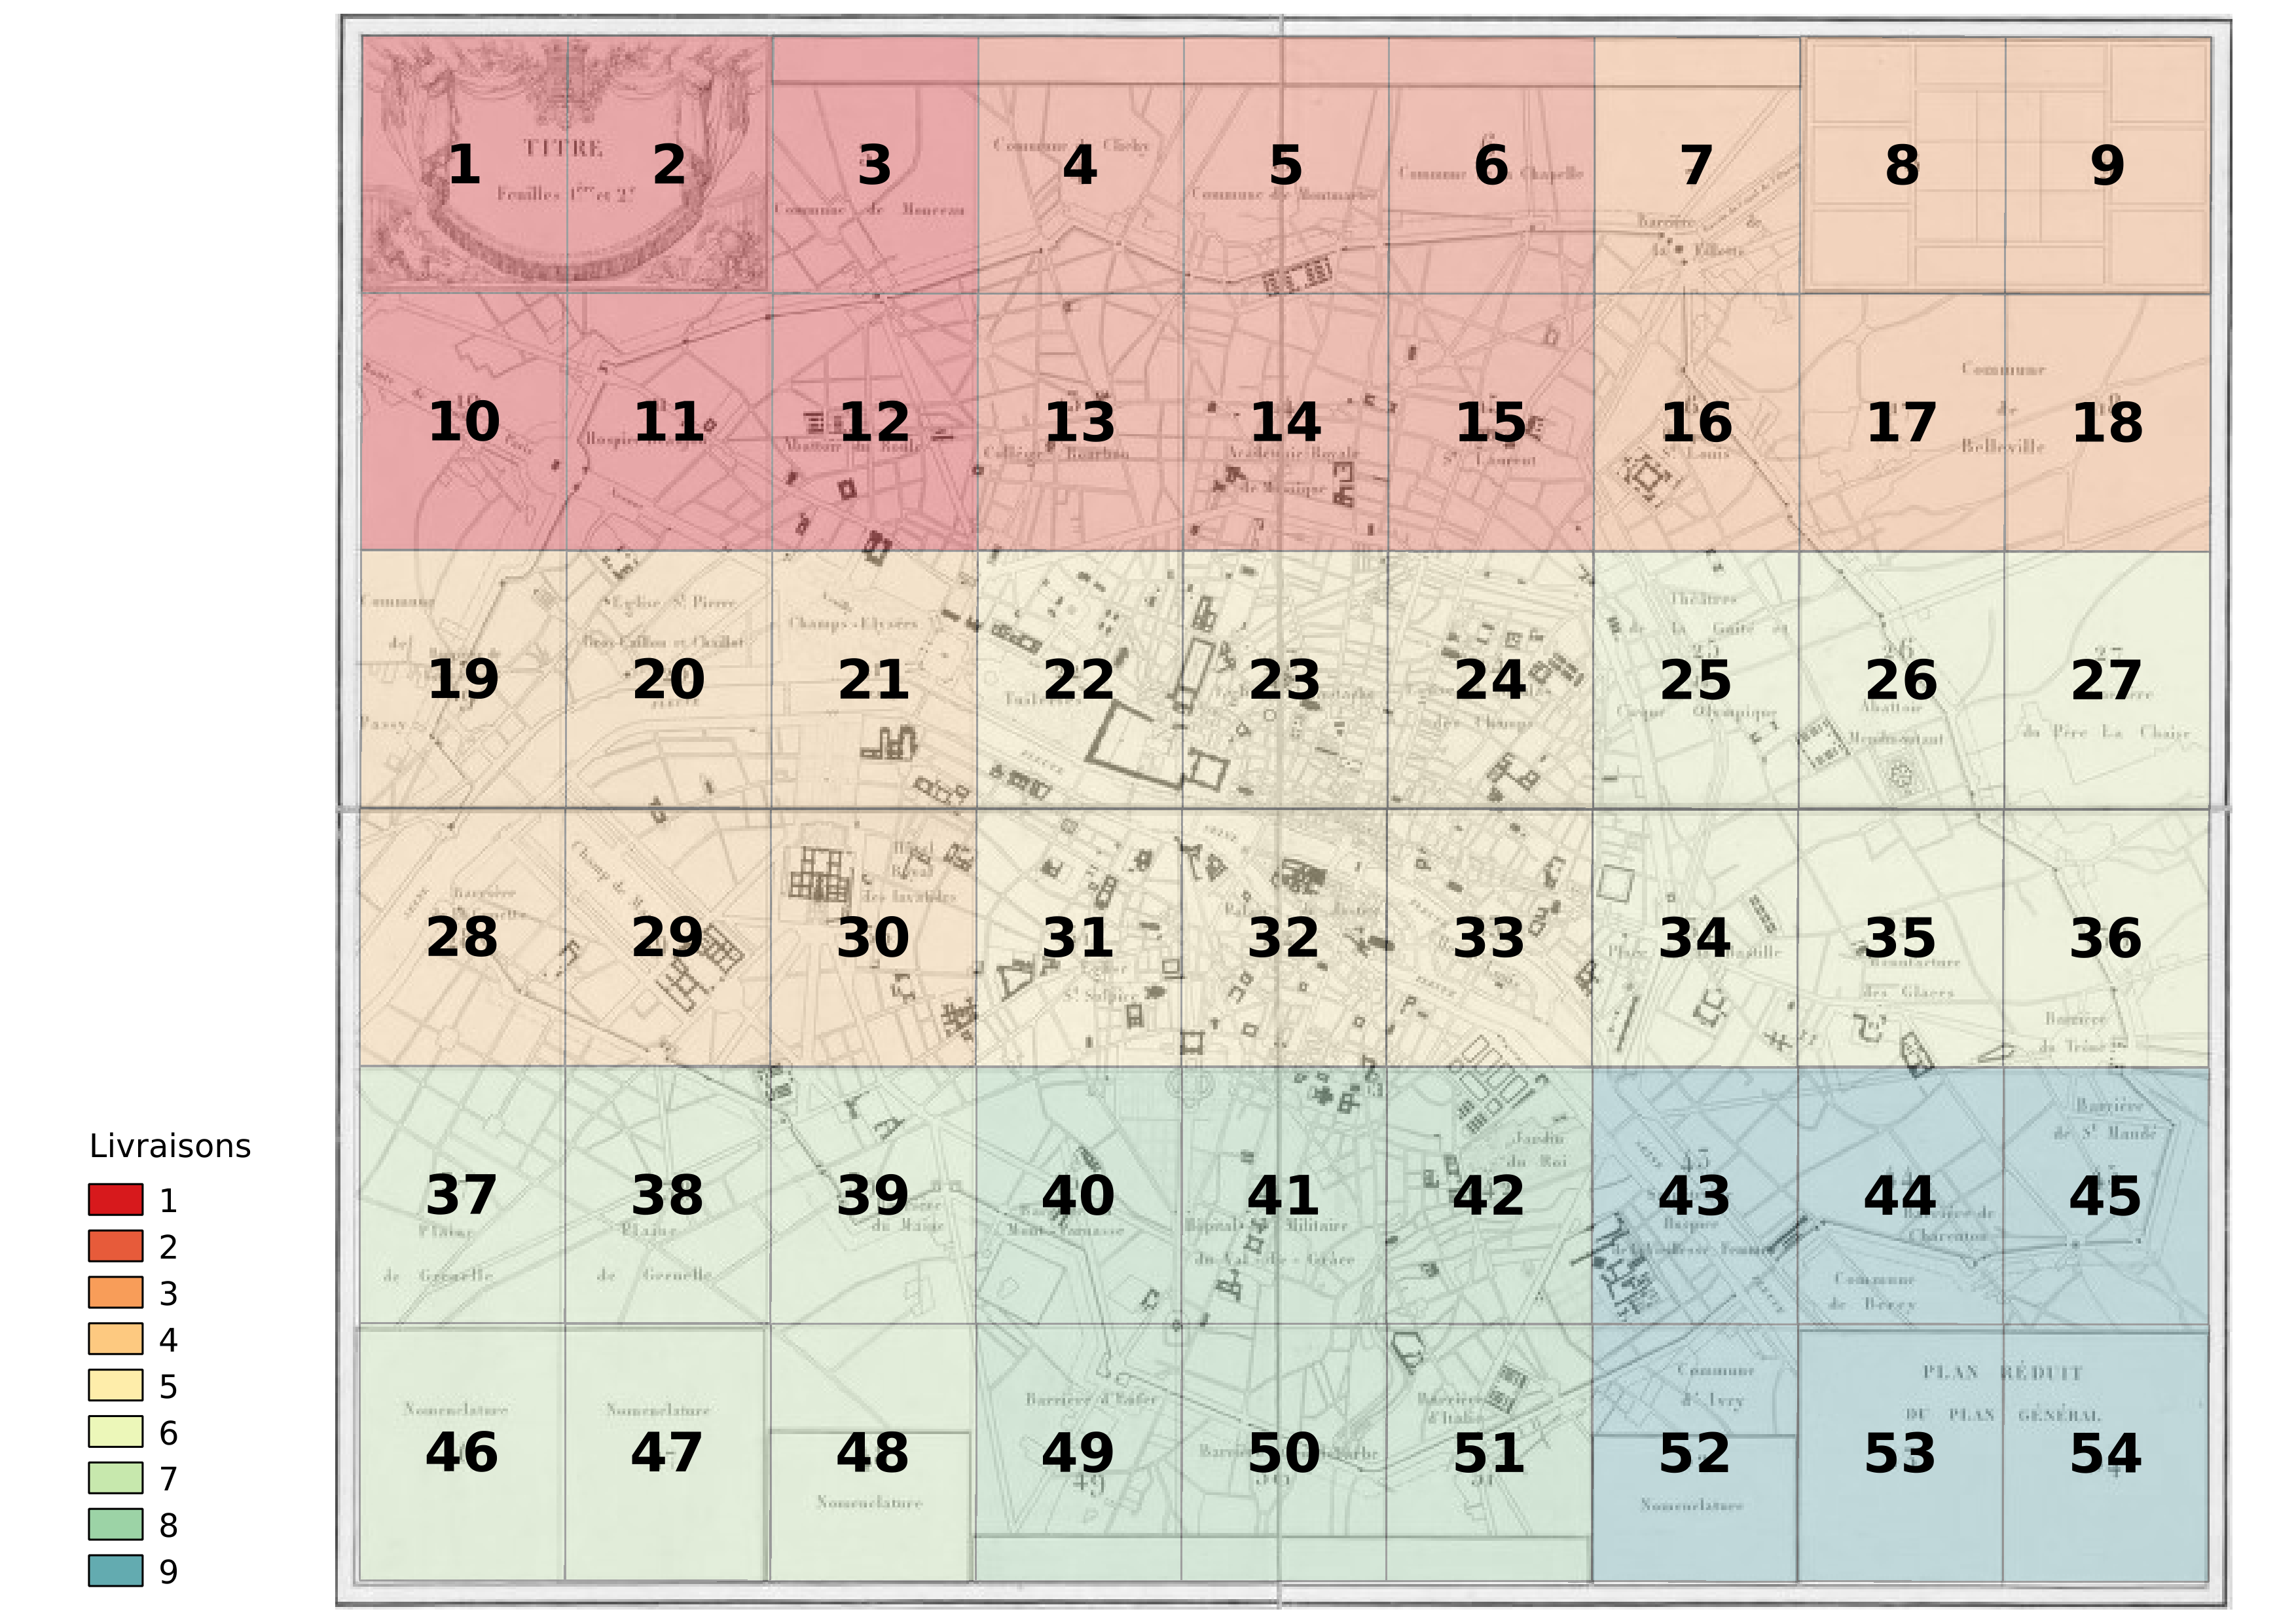
\includegraphics[width=1\textwidth]{assemblage_jacoubet.png} 
	\caption{Index des planches de l'atlas g�n�ral de Jacoubet, trac� sur le plan d'assemblage, qui en constitue les feuilles 8 et 9.}
	\label{figure:assemblage_jacoubet}
\end{figure}

La gravure r�alis�e par Antony-Gr�goire Niquet est efficace puisque le 13 janvier 1827 para�t la premi�re livraison du nouvel atlas\footnote{En r�alit�, il s'agit de la seconde livraison pr�vue par Jacoubet, soient les feuilles 4, 5, 6, 13, 14 et 15, la premi�re ayant pris du retard.
Cette livraison est la seule qui soit parvenue jusqu'� nous dans son �tat originel.
Elle se trouve actuellement � la Biblioth�que Historique de la Ville de Paris.
\citep{BHVPFMAT12}}, suivie dans le courant de l'ann�e par deux autres livraisons.
Bien que nous n'ayons trouv� trace des autres livraisons, rien ne laisse croire que le rythme ait baiss� jusqu'en fin d'ann�e 1828.
Avec un rythme de trois livraisons par an, � la fin de l'ann�e 1828 six livraisons du plan auraient �t� grav�es et publi�es.
\paragraph{}
Pourtant, cette publication n'est pas sans incident.
En effet, d�s 1826 et l'apparition du prospectus, M\up{me} Chavagnac, soup�onnant Jacoubet de publier une nouvelle version du plan de Verniquet qu'il lui avait vendue l'ann�e pr�c�dente, l'assigne devant le tribunal de premi�re instance de la Seine pour non respect du contrat sur le plan de 1825.
En effet, il n'�chappe certainement pas � M\up{me} Chavagnac qu'il est difficilement envisageable qu'un nouveau plan de Paris, � une �chelle aussi grande, ait put �tre enti�rement r�alis� en quelques mois l� o� 6 ans avaient �t� n�cessaire � Verniquet et 14 ans � Vasserot, d'autant plus qu'il publie ce nouveau plan � la suite de celui qu'il lui a c�d�.
De plus, l'un des auteurs du plan, Mangot, avait entre temps vendu frauduleusement les 72 feuilles dessin�es de l'atlas de Verniquet en possession du bureau des plans\footnote{Fort heureusement, la pr�fecture r�cup�rera les plans avant qu'ils soient vendus et Mangot sera limog� en 1831.}, jetant ainsi quelques doutes sur les pratiques des g�om�tres et architectes du bureau.
\paragraph{}
Le 20 d�cembre 1828 M\up{me} Chavagnac obtient gain de cause et Jacoubet se voit condamn� � la cessation de la publication et � la destruction des minutes et des cuivres.
Faisant appel, une commission d'enqu�te est nomm�e le 7 ao�t 1829 pour �tudier le plan et d�cider s'il s'agit d'une {\oe}uvre originale ou d'une nouvelle publication du plan de 1825, mais, en attendant son rapport, l'interdiction de publication est maintenue.
Finalement, le 8 mars 1830 la commission conclut que~:
\begin{itemize}
 \item L'atlas n'est pas une version � une autre �chelle du plan de Verniquet.
 \item Ce n'est pas non plus une nouvelle version du plan r�duit publi� en 1825.
 \item L'atlas a �t� effectu� sur une nouvelle triangulation et, par cons�quent, il est totalement original.
\end{itemize}
Jacoubet sort donc vainqueur de ce proc�s et reprend aussit�t la publication de son atlas.
Il ne rencontrera plus de probl�mes majeurs, hormis une soustraction momentan�e des cuivres par son graveur Niquet en 1833, ce qui l'incitera � changer de graveur et � choisir Louis-Marin Bonnet pour le remplacer \citep[p. 4]{GazetteTribunaux18330724}.
La gravure de toutes les planches semble avoir �t� termin�e autour de 1834, Jacoubet affirmant lui-m�me qu'a cette date son atlas \emph{�tait termin�, 
ou presque} \citep[p. 2]{GazetteTribunaux18421111}.
Finalement, il publiera courant 1836 la totalit� de son plan sous la forme d'un grand livre, auquel il ajoutera les �l�ments suivants~:
\begin{itemize}
 \item Les plans de Paris � diverses �poques, tr�s inexacts~: \emph{sous la domination Romaine}, \emph{sous le r�gne de Fran�ois I\up{er}}, \emph{sous le r�gne de Louis XIII}, \emph{sous le r�gne de Philippe Auguste} et \emph{sous Louis Philippe I\up{er}}.
\item Les plans des cimeti�res de Paris (incorpor�s au plan).
\item Le plan r�sumant la triangulation ayant permis le lev� de l'atlas.
\end{itemize}

\myparagraph{1836~: publication de l'atlas et critique de la datation}
Ainsi donc, l'atlas de Jacoubet semble, tout du moins dans sa phase de lev� et de gravure, plus ancien que ce qui est g�n�ralement avanc� (1827-1840 pour Jeanne Pronteau \citep{Pronteau1986}, 1827-1839 pour Pierre Pinon \citep[p. 94]{Pinon2004}).
Le relev� du plan daterait donc de la p�riode 1824-1826, et sa gravure s'�chelonnerait principalement entre 1827 et 1834.
Finalement, le plan sera publi� sous forme d'atlas -c'est � dire d'un livre reli� contenant toutes les planches-  en 1836, tel que l'indiquent effectivement les planches 1 et 2 \footnote{Jeanne Pronteau note cependant que cette date est sans doute fictive, les armoiries dessin�es sur la m�me planche �tant celles de la Restauration.} et comme en t�moigne �galement Jacoubet \citep[p. 2]{GazetteTribunaux18421111}.
\paragraph{}
Cependant, la datation que nous avons �tablie am�ne une seconde question~: si le plan a effectivement �t� trac� vers 1825, le rythme des transformations de Paris le rendent d�j� obsol�te � sa publication en 1836.
Il para�t peu vraisemblable que Jacoubet, qui voulait faire de son atlas le nouveau \emph{Grand Plan de Paris} dans lequel tous les projets de voirie figureraient, ait publi� le plan dat� de 10 ans sans l'avoir jamais mis � jour, y avoir report� les nouveaux projets et percements.
Il publiera d'ailleurs plusieurs fois son plan dans les ann�es suivantes en grand format (1838,1841) ou en r�duction au 1/10.000\up{e} d�s 1836.
Il en fera une mise � jour compl�te en 1841.
On trouve une version grav�e des trois premi�res livraisons en 1833, soit 6 ans apr�s leur premi�re parution \citep{MAPPartialJacoubet1833}\footnote{Cette version, conserv�e � la BNF \citep{MAPPartialJacoubet1833}, ne contient cependant que les planches 3 � 7, 10 � 12 et 16 � 18.
Il manque donc les planches 1,2, 8, 9 ,13, 14 et 15.}.
Si l'atlas a �t� modifi� en cours m�me de publication, la chronologie �tablie jusqu'ici est alors tout � fait insuffisante pour conna�tre le v�ritable temps de r�alisation du plan.
Plus encore, il nous faut d�terminer si le plan a subi des mises � jours globales, o� si chaque planche a suivi une trajectoire diff�rente.
Seule une seconde analyse fond�e sur le contenu de l'atlas peut r�pondre � ces questions.


\subsection{Datation fine}
\myparagraph{Datation par planches}
Afin de d�terminer l'intervalle pendant lequel chaque planche a �t� dessin�e puis grav�e et ainsi v�rifier si les livraisons sont coh�rentes ou s'il y a eu des mises � jour ponctuelles entre 1827 et 1836, nous avons analys� le contenu de chacune des planches de la premi�re �dition de l'atlas dat�e de 1836.
La m�thodologie adopt�e pour fixer les bornes de chaque intervalle est la suivante~: 
\begin{itemize}
 \item La borne inf�rieure peut �tre approch�e en connaissant les dates de cr�ation des �l�ments repr�sent�s.
Par exemple, si un alignement est trac� sur une planche alors elle a �t� grav�e apr�s la date de l'ordonnance d'alignement.
 \item La borne sup�rieure est trouv�e de la fa�on inverse.
Ainsi, lorsqu'une d�cision de voirie est prise et non repr�sent�e sur la planche, cela signifie que cette derni�re est ant�rieure.
Cette �tape est cependant plus fragile car elle est sensible aux �ventuels oublis de l'auteur, mais aussi car certains percements sont omis car r�alis�s sans autorisation officielle (C'est le cas en particulier � l'est de Paris avec les rues Gambrey et Pierre Lev�e, mais aussi parfois � l'ouest comme pour la rue de Milan).
\end{itemize}
Il est aussi n�cessaire de choisir quelles informations sont suffisamment fiables pour guider la fixation des bornes temporelles.
Ici, nous nous sommes appuy� sur le prospectus de Jacoubet qui donnait une importance particuli�re � la repr�sentation des ordonnances de voirie.
Ainsi, � partir des objectifs du plan d'origine, nous avons choisi de nous appuyer sur les �l�ments pr�sent�s dans le tableau ci-dessous.
\begin{table}[ht!]
\begin{tabular}{|p{3.6cm}|p{10.5cm}|}
\hline
 Alignements et percements & Rappelons que le plan rapporte \emph{tous les projets de percements, ainsi que les alignements arr�t�s par ordonnance royale}.
Ainsi, tous les �largissements, projets de percements et d'ouvertures sont repr�sent�s sur le plan d�s lors qu'ils sont d�cid�s par ordonnance royale ou d�cret, dont les dates exactes peuvent �tre retrouv�es.\\
\hline
D�nominations & Les changements de noms des rues et b�timents, lorsqu'ils r�sultent de d�cisions royales ou pr�fectorales, sont report�s sur le plan.
Cette indication est pr�cieuse pour un atlas qui a travers� une r�volution ayant amen� divers changements de d�nominations des rues (Lafayette, place du Panth�on, etc.)\\
\hline
B�timents publics & Les b�timents publics repr�sent�s sur le plan sont soit existants, soit parties de projets officiels dont la date de d�cision peut �galement �tre retrouv�e.\\
\hline
\end{tabular}
\caption{Types d'�v�nements affectant Paris ayant permis de dater les planches de l'atlas de Jacoubet, tri�s par ordre d�croissant de fiabilit�.}
\label{table:types_evts_datation_fine_jacoubet}
\end{table}

Notons que, puisque le plan rapporte les projets officiels et non ce qui est d�j� effectu�, il peut nous induire en erreur.
Par exemple, les plans de l'H�tel de Ville et de la Biblioth�que de Roi sont trac�s bien qu'ils n'aient jamais �t� r�alis�s en l'�tat.
De m�me, certaines rues telle celle de Munich, partie du lotissement de l'Europe, sont dessin�es mais n'ont jamais �t� ouvertes.
\\
Nous avons choisi, pour dater les rues, projets et ordonnances, de nous appuyer uniquement sur des sources officielles~:
\begin{itemize}
 \item Les \emph{Dictionnaires Historiques des Rues de Paris} par les fr�res Lazare, dat�s de 1844 et 1855 \citep{Lazare1844, Lazare1855}.
 \item Le \emph{Recueil g�n�ral des lois et des arr�ts} contenant les ordonnances royales
 \item La nomenclature des rues de Paris diffus�e en 2012 par la Mairie de Paris\footnote{\url{http://parisdata.opendatasoft.com/explore/dataset/voiesactuellesparis2012}}.
\end{itemize}
Nous avons en outre d�cid� de ne pas nous appuyer sur d'autres plans contemporains qui, par comparaison, auraient permis de pr�ciser les dates des rues.
En effet, la plupart des autres plans de l'�poque sont tr�s peu fiables, parce que, face au rythme de transformation de Paris et pour �viter une trop rapide obsolescence, ils repr�sentent en avance de nombreux percements.
Il est courant qu'un plan contienne le trac� de rues ayant �t� cr��es plusieurs ann�es apr�s sa parution, ou bien m�me de rues jamais perc�es.
C'est le cas des plans de Girard \citep{MAPGirard1830}, Achin \citep{MAPAchin1825} ou Tardieu \citep{MAPTardieu1838}.
Seule la seconde �dition de l'atlas de Jacoubet, publi�e vers 1839, a �t� utilis�e pour discriminer les projets de voirie d�cid�s avant 1836 mais pas encore effectu�s en 1839.
\paragraph{}
Le r�sultat de cette analyse est pr�sent� au sein du tableau \ref{table:datation_jacoubet_fin}, qui fait appara�tre pour chaque planche l'intervalle temporel de son dessin, que nous obtenons � partir d'une somme d'indices temporels rassembl�s dans l'annexe \ref{annexe:detailsJacoubet}.

Pour chaque planche, l'intervalle temporel \colorbox{possibilite}{\protect\phantom{aa}} d�crivant la p�riode de son possible dessin est d�duit d'une somme d'�v�nements dat�s concernant l'urbanisme parisien~:percement de rues, alignements, construction,etc.
Les types d'�v�nements sont d�crits dans le tableau \ref{table:types_evts_datation_fine_jacoubet}, et la liste compl�te est fournie dans l'annexe \ref{annexe:detailsJacoubet}.
Ces �v�nements sont de deux types.
Les premiers not�s \textcolor{arrow}{$\blacktriangleright$} sont dessin�s sur la planche et sont donc consid�r�s comme ant�rieurs au dessin.
Les seconds, not�s \textcolor{arrowleft}{$\blacktriangleleft$}, ne sont pas repr�sent�s sur la planche et sont donc consid�r�s post�rieurs au dessin.
Ces deux cat�gories d'�v�nements permettent de d�finir les bornes inf�rieures et sup�rieures de l'intervalle temporel pendant lequel la planche a pu �tre dessin�e puis grav�e.
L'�cart temporel entre un �v�nement, g�n�ralement dat� au jour pr�s, et son report sur la carte nous est inconnu, produisant une incertitude sur la position des bornes au sein d'une ann�e.
Cette incertitude est repr�sent�e dans le tableau par le couleur \colorbox{incertitude}{\protect\phantom{aa}}.
Enfin, certains �v�nements se contredisent, ce qui peut arriver dans le cas de corrections partielles d'une planche ou d'oublis.
Ils se trouvent indiqu�s par la couleur \colorbox{incoherence}{\protect\phantom{aa}}.
Les bornes de certaines planches n'ayant pas pu �tre d�termin�es par manque d'informations, en particulier dans les zones p�riph�riques, nous avons arbitrairement fix� un minimum et un maximum, respectivement 1825 et 1836, la premi�re date correspondant au d�but de la r�alisation du grand atlas et la seconde � son ann�e de publication.
Seules les planches ayant un contenu cartographique sont repr�sent�es.

\begin{longtable}{|c|c c c c c c c c c c c c|}
\caption{Datation des planches de l'atlas de Jacoubet commenc� en 1825 et publi� en 1836, rassembl�es par livraison.}\label{table:datation_jacoubet_fin}\\
\hline
\multicolumn{1}{|c}{ }&\multicolumn{12}{|c|}{Ann�es}\\
Planches&1825&26&27&28&29&30&31&32&33&34&35&36 \\
\hline
\endfirsthead
\hline
\multicolumn{1}{|c}{ }&\multicolumn{12}{|c|}{Ann�es}\\
Planches&1825&26&27&28&29&30&31&32&33&34&35&36 \\
\hline
\endhead

3 &\cellcolor{possibilite}{} &\cellcolor{possibilite}{} & \cellcolor{possibilite}{} & \cellcolor{incertitude}{\textbf{\textcolor{arrowleft}{$ \blacktriangleleft$} }} &\cellcolor{impossibilite}{} &\cellcolor{impossibilite}{\textbf{\textcolor{arrowleft}{$ \blacktriangleleft$} }} &\cellcolor{impossibilite}{} &\cellcolor{impossibilite}{} &\cellcolor{impossibilite}{} &\cellcolor{impossibilite}{} &\cellcolor{impossibilite}{} &\cellcolor{impossibilite}{} \\

10 &\cellcolor{incertitude}{\textcolor{arrow}{$\blacktriangleright$}} &\cellcolor{possibilite}{}& \cellcolor{possibilite}{} & \cellcolor{possibilite}{} &\cellcolor{possibilite}{} &\cellcolor{possibilite}{} &\cellcolor{possibilite}{} &\cellcolor{possibilite}{} &\cellcolor{possibilite}{} &\cellcolor{possibilite}{} &\cellcolor{possibilite}{} &\cellcolor{possibilite}{} \\

11 &\cellcolor{impossibilite}{\textcolor{arrow}{$\blacktriangleright$}} &\cellcolor{impossibilite}{}& \cellcolor{impossibilite}{} & \cellcolor{impossibilite}{} &\cellcolor{incertitude}{\textcolor{arrow}{$\blacktriangleright$}} &\cellcolor{possibilite}{} &\cellcolor{possibilite}{} &\cellcolor{possibilite}{} &\cellcolor{possibilite}{} &\cellcolor{possibilite}{} &\cellcolor{possibilite}{} &\cellcolor{incertitude}{\textbf{\textcolor{arrowleft}{$ \blacktriangleleft$} }} \\

12 &\cellcolor{impossibilite}{} &\cellcolor{incertitude}{\textcolor{arrow}{$\blacktriangleright$}}& \cellcolor{possibilite}{} & \cellcolor{possibilite}{} &\cellcolor{possibilite}{} &\cellcolor{possibilite}{} &\cellcolor{possibilite}{} &\cellcolor{possibilite}{} &\cellcolor{possibilite}{} &\cellcolor{possibilite}{} &\cellcolor{possibilite}{} &\cellcolor{incertitude}{\textbf{\textcolor{arrowleft}{$ \blacktriangleleft$} }} \\

\hline\hline
4 &\cellcolor{impossibilite}{} &\cellcolor{incertitude}{\textcolor{arrow}{$\blacktriangleright$}}& \cellcolor{possibilite}{} & \cellcolor{possibilite}{} &\cellcolor{possibilite}{} &\cellcolor{possibilite}{} &\cellcolor{possibilite}{} &\cellcolor{possibilite}{} &\cellcolor{possibilite}{} &\cellcolor{possibilite}{} &\cellcolor{possibilite}{} &\cellcolor{incertitude}{\textbf{\textcolor{arrowleft}{$ \blacktriangleleft$} }} \\

5 &\cellcolor{impossibilite}{\textcolor{arrow}{$\blacktriangleright$}} &\cellcolor{incertitude}{\textcolor{arrow}{$\blacktriangleright$}}& \cellcolor{possibilite}{} & \cellcolor{possibilite}{} &\cellcolor{possibilite}{} &\cellcolor{possibilite}{} &\cellcolor{possibilite}{} &\cellcolor{possibilite}{} &\cellcolor{incertitude}{\textbf{\textcolor{arrowleft}{$ \blacktriangleleft$} }} &\cellcolor{impossibilite}{} &\cellcolor{impossibilite}{} &\cellcolor{impossibilite}{} \\

6 &\cellcolor{impossibilite}{} &\cellcolor{impossibilite}{\textcolor{arrow}{$\blacktriangleright$}}& \cellcolor{incertitude}{\textcolor{arrow}{$\blacktriangleright$}} & \cellcolor{possibilite}{} &\cellcolor{possibilite}{} &\cellcolor{possibilite}{} &\cellcolor{possibilite}{} &\cellcolor{possibilite}{} &\cellcolor{possibilite}{} &\cellcolor{possibilite}{} &\cellcolor{possibilite}{} &\cellcolor{possibilite}{} \\

13 &\cellcolor{impossibilite}{} &\cellcolor{impossibilite}{\textcolor{arrow}{$\blacktriangleright$}}& \cellcolor{incertitude}{\textcolor{arrow}{$\blacktriangleright$}} & \cellcolor{possibilite}{} &\cellcolor{possibilite}{} &\cellcolor{incertitude}{\textbf{\textcolor{arrowleft}{$ \blacktriangleleft$} }} &\cellcolor{impossibilite}{\textbf{\textcolor{arrowleft}{$ \blacktriangleleft$} }} &\cellcolor{impossibilite}{} &\cellcolor{impossibilite}{} &\cellcolor{impossibilite}{} &\cellcolor{impossibilite}{} &\cellcolor{impossibilite}{} \\

14 &\cellcolor{impossibilite}{} &\cellcolor{impossibilite}{\textcolor{arrow}{$\blacktriangleright$}}& \cellcolor{impossibilite}{} & \cellcolor{impossibilite}{} &\cellcolor{impossibilite}{} &\cellcolor{incertitude}{\textcolor{arrow}{$\blacktriangleright$}\textcolor{arrow}{$\blacktriangleright$}} &\cellcolor{incertitude}{\textbf{\textcolor{arrowleft}{$ \blacktriangleleft$} }}&\cellcolor{impossibilite}{\textbf{\textcolor{arrowleft}{$ \blacktriangleleft$} }}&\cellcolor{impossibilite}{} &\cellcolor{impossibilite}{} &\cellcolor{impossibilite}{} &\cellcolor{impossibilite}{} \\

15 &\cellcolor{impossibilite}{} &\cellcolor{impossibilite}{}& \cellcolor{impossibilite}{\textcolor{arrow}{$\blacktriangleright$}} & \cellcolor{impossibilite}{} &\cellcolor{incertitude}{\textcolor{arrow}{$\blacktriangleright$}} &\cellcolor{possibilite}{} &\cellcolor{possibilite}{}&\cellcolor{incertitude}{\textbf{\textcolor{arrowleft}{$ \blacktriangleleft$} }}&\cellcolor{impossibilite}{} &\cellcolor{impossibilite}{} &\cellcolor{impossibilite}{} &\cellcolor{impossibilite}{\textbf{\textcolor{arrowleft}{$ \blacktriangleleft$} }} \\

\hline\hline

7 &\cellcolor{impossibilite}{} &\cellcolor{impossibilite}{}& \cellcolor{impossibilite}{} & \cellcolor{impossibilite}{} &\cellcolor{impossibilite}{} &\cellcolor{incertitude}{\textcolor{arrow}{$\blacktriangleright$}} &\cellcolor{possibilite}{} &\cellcolor{possibilite}{} &\cellcolor{possibilite}{} &\cellcolor{possibilite}{} &\cellcolor{possibilite}{} &\cellcolor{possibilite}{} \\


16 &\cellcolor{impossibilite}{\textcolor{arrow}{$\blacktriangleright$}} &\cellcolor{impossibilite}{\textcolor{arrow}{$\blacktriangleright$}}& \cellcolor{impossibilite}{\textcolor{arrow}{$\blacktriangleright$}} & \cellcolor{impossibilite}{} &\cellcolor{impossibilite}{} &\cellcolor{incertitude}{\textcolor{arrow}{$\blacktriangleright$}} &\cellcolor{possibilite}{} &\cellcolor{possibilite}{} &\cellcolor{possibilite}{} &\cellcolor{possibilite}{} &\cellcolor{possibilite}{} &\cellcolor{incertitude}{\textbf{\textcolor{arrowleft}{$ \blacktriangleleft$} }} \\

17 &\cellcolor{possibilite}{} &\cellcolor{possibilite}{}& \cellcolor{possibilite}{} & \cellcolor{possibilite}{} &\cellcolor{possibilite}{} &\cellcolor{possibilite}{} &\cellcolor{possibilite}{} &\cellcolor{possibilite}{} &\cellcolor{possibilite}{} &\cellcolor{possibilite}{} &\cellcolor{possibilite}{} &\cellcolor{possibilite}{} \\

18 &\cellcolor{possibilite}{} &\cellcolor{possibilite}{}& \cellcolor{possibilite}{} & \cellcolor{possibilite}{} &\cellcolor{possibilite}{} &\cellcolor{possibilite}{} &\cellcolor{possibilite}{} &\cellcolor{possibilite}{} &\cellcolor{possibilite}{} &\cellcolor{possibilite}{} &\cellcolor{possibilite}{} &\cellcolor{possibilite}{} \\

\hline\hline

19 &\cellcolor{impossibilite}{} &\cellcolor{impossibilite}{}& \cellcolor{impossibilite}{} & \cellcolor{impossibilite}{} &\cellcolor{impossibilite}{} &\cellcolor{impossibilite}{} &\cellcolor{impossibilite}{} &\cellcolor{incertitude}{\textcolor{arrow}{$\blacktriangleright$}} &\cellcolor{possibilite}{} &\cellcolor{possibilite}{} &\cellcolor{possibilite}{} &\cellcolor{possibilite}{} \\

20 &\cellcolor{impossibilite}{} &\cellcolor{impossibilite}{}& \cellcolor{impossibilite}{} & \cellcolor{impossibilite}{} &\cellcolor{impossibilite}{} &\cellcolor{impossibilite}{} &\cellcolor{impossibilite}{} &\cellcolor{impossibilite}{\textcolor{arrow}{$\blacktriangleright$}} &\cellcolor{incertitude}{\textcolor{arrow}{$\blacktriangleright$}} &\cellcolor{possibilite}{} &\cellcolor{possibilite}{} &\cellcolor{possibilite}{} \\

21 &\cellcolor{impossibilite}{} &\cellcolor{impossibilite}{}& \cellcolor{incoherence}{\textbf{\textcolor{arrowleft}{$ \blacktriangleleft$} }} & \cellcolor{incoherence}{\textcolor{arrow}{$\blacktriangleright$}} &\cellcolor{incoherence}{\textcolor{arrow}{$\blacktriangleright$}} &\cellcolor{incoherence}{\textcolor{arrow}{$\blacktriangleright$}} &\cellcolor{impossibilite}{} &\cellcolor{impossibilite}{} &\cellcolor{impossibilite}{} &\cellcolor{impossibilite}{} &\cellcolor{impossibilite}{} &\cellcolor{impossibilite}{\textbf{\textcolor{arrowleft}{$ \blacktriangleleft$} }} \\

28 &\cellcolor{impossibilite}{} &\cellcolor{incertitude}{\textcolor{arrow}{$\blacktriangleright$}}& \cellcolor{possibilite}{} & \cellcolor{possibilite}{} &\cellcolor{possibilite}{} &\cellcolor{incertitude}{\textbf{\textcolor{arrowleft}{$ \blacktriangleleft$} }} &\cellcolor{impossibilite}{} &\cellcolor{impossibilite}{} &\cellcolor{impossibilite}{} &\cellcolor{impossibilite}{} &\cellcolor{impossibilite}{} &\cellcolor{impossibilite}{} \\

29 &\cellcolor{incertitude}{\textcolor{arrow}{$\blacktriangleright$}} &\cellcolor{possibilite}{}& \cellcolor{possibilite}{} & \cellcolor{possibilite}{} &\cellcolor{possibilite}{} &\cellcolor{possibilite}{} &\cellcolor{possibilite}{} &\cellcolor{possibilite}{} &\cellcolor{possibilite}{} &\cellcolor{possibilite}{} &\cellcolor{possibilite}{} &\cellcolor{possibilite}{} \\


30 &\cellcolor{impossibilite}{} &\cellcolor{impossibilite}{}& \cellcolor{incertitude}{\textcolor{arrow}{$\blacktriangleright$}} & \cellcolor{possibilite}{} &\cellcolor{possibilite}{} &\cellcolor{possibilite}{} &\cellcolor{possibilite}{} &\cellcolor{possibilite}{} &\cellcolor{possibilite}{} &\cellcolor{possibilite}{} &\cellcolor{possibilite}{} &\cellcolor{possibilite}{} \\

\hline\hline


22&\cellcolor{impossibilite}{} &\cellcolor{impossibilite}{}& \cellcolor{impossibilite}{} & \cellcolor{impossibilite}{\textcolor{arrow}{$\blacktriangleright$}} &\cellcolor{impossibilite}{} &\cellcolor{impossibilite}{} &\cellcolor{impossibilite}{} &\cellcolor{incertitude}{\textcolor{arrow}{$\blacktriangleright$}} &\cellcolor{possibilite}{} &\cellcolor{incertitude}{\textbf{\textcolor{arrowleft}{$ \blacktriangleleft$} }} &\cellcolor{impossibilite}{} &\cellcolor{impossibilite}{} \\

23&\cellcolor{impossibilite}{} &\cellcolor{impossibilite}{}& \cellcolor{impossibilite}{} & \cellcolor{impossibilite}{} &\cellcolor{impossibilite}{} &\cellcolor{impossibilite}{} &\cellcolor{impossibilite}{} &\cellcolor{impossibilite}{} &\cellcolor{incertitude}{\textcolor{arrow}{$\blacktriangleright$}} &\cellcolor{possibilite}{} &\cellcolor{possibilite}{} &\cellcolor{incertitude}{\textbf{\textcolor{arrowleft}{$ \blacktriangleleft$} }} \\

24&\cellcolor{impossibilite}{} &\cellcolor{incoherence}{\textcolor{arrow}{$\blacktriangleright$}\textbf{\textcolor{arrowleft}{$ \blacktriangleleft$} }}& \cellcolor{incoherence}{} & \cellcolor{incoherence}{\textcolor{arrow}{$\blacktriangleright$}} &\cellcolor{incoherence}{\textcolor{arrow}{$\blacktriangleright$}\textbf{\textcolor{arrowleft}{$ \blacktriangleleft$} }} &\cellcolor{incoherence}{} &\cellcolor{incoherence}{} &\cellcolor{incoherence}{} &\cellcolor{incoherence}{\textcolor{arrow}{$\blacktriangleright$}\textbf{\textcolor{arrow}{$ \blacktriangleleft$} }} &\cellcolor{impossibilite}{} &\cellcolor{impossibilite}{} &\cellcolor{impossibilite}{\textbf{\textcolor{arrowleft}{$ \blacktriangleleft$} }} \\

31&\cellcolor{impossibilite}{} &\cellcolor{impossibilite}{}& \cellcolor{impossibilite}{} & \cellcolor{impossibilite}{} &\cellcolor{impossibilite}{} &\cellcolor{impossibilite}{} &\cellcolor{impossibilite}{\textcolor{arrow}{$\blacktriangleright$}} &\cellcolor{impossibilite}{} &\cellcolor{impossibilite}{} &\cellcolor{incertitude}{\textcolor{arrow}{$\blacktriangleright$}} &\cellcolor{possibilite}{} &\cellcolor{possibilite}{} \\

32&\cellcolor{impossibilite}{} &\cellcolor{impossibilite}{}& \cellcolor{impossibilite}{} & \cellcolor{impossibilite}{} &\cellcolor{impossibilite}{} &\cellcolor{impossibilite}{} &\cellcolor{impossibilite}{\textcolor{arrow}{$\blacktriangleright$}} &\cellcolor{impossibilite}{} &\cellcolor{impossibilite}{} &\cellcolor{impossibilite}{} &\cellcolor{incertitude}{\textcolor{arrow}{$\blacktriangleright$}} &\cellcolor{possibilite}{} \\

33&\cellcolor{impossibilite}{} &\cellcolor{impossibilite}{}& \cellcolor{impossibilite}{} & \cellcolor{impossibilite}{} &\cellcolor{impossibilite}{} &\cellcolor{impossibilite}{\textcolor{arrow}{$\blacktriangleright$}} &\cellcolor{impossibilite}{} &\cellcolor{impossibilite}{} &\cellcolor{impossibilite}{\textcolor{arrow}{$\blacktriangleright$}} &\cellcolor{incertitude}{\textcolor{arrow}{$\blacktriangleright$}} &\cellcolor{possibilite}{} &\cellcolor{incertitude}{\textbf{\textcolor{arrowleft}{$ \blacktriangleleft$} }} \\

\hline\hline

25&\cellcolor{impossibilite}{} &\cellcolor{impossibilite}{}& \cellcolor{impossibilite}{} & \cellcolor{impossibilite}{} &\cellcolor{incertitude}{\textcolor{arrow}{$\blacktriangleright$}\textbf{\textcolor{arrowleft}{$ \blacktriangleleft$} }} &\cellcolor{impossibilite}{} &\cellcolor{impossibilite}{} &\cellcolor{impossibilite}{} &\cellcolor{impossibilite}{} &\cellcolor{impossibilite}{} &\cellcolor{impossibilite}{\textbf{\textcolor{arrowleft}{$ \blacktriangleleft$} }} &\cellcolor{impossibilite}{} \\

26&\cellcolor{incertitude}{\textcolor{arrow}{$ \blacktriangleright$} } &\cellcolor{possibilite}{}& \cellcolor{possibilite}{} & \cellcolor{possibilite}{} &\cellcolor{possibilite}{} &\cellcolor{incertitude}{\textbf{\textcolor{arrowleft}{$ \blacktriangleleft$} }} &\cellcolor{impossibilite}{} &\cellcolor{impossibilite}{} &\cellcolor{impossibilite}{} &\cellcolor{impossibilite}{} &\cellcolor{impossibilite}{} &\cellcolor{impossibilite}{} \\

27&\cellcolor{possibilite}{} &\cellcolor{possibilite}{}& \cellcolor{possibilite}{} & \cellcolor{possibilite}{} &\cellcolor{possibilite}{} &\cellcolor{possibilite}{} &\cellcolor{possibilite}{} &\cellcolor{possibilite}{} &\cellcolor{possibilite}{} &\cellcolor{possibilite}{} &\cellcolor{possibilite}{} &\cellcolor{possibilite}{} \\

34&\cellcolor{impossibilite}{} &\cellcolor{impossibilite}{}& \cellcolor{incoherence}{\textcolor{arrow}{$\blacktriangleright$}\textbf{\textcolor{arrowleft}{$ \blacktriangleleft$} }} & \cellcolor{incoherence}{\textbf{\textcolor{arrowleft}{$ \blacktriangleleft$} }} &\cellcolor{incoherence}{\textcolor{arrow}{$\blacktriangleright$}} &\cellcolor{incoherence}{} &\cellcolor{incoherence}{\textbf{\textcolor{arrowleft}{$ \blacktriangleleft$} }} &\cellcolor{incoherence}{} &\cellcolor{incoherence}{} &\cellcolor{incoherence}{\textcolor{arrow}{$\blacktriangleright$}} &\cellcolor{impossibilite}{} &\cellcolor{impossibilite}{} \\

35&\cellcolor{impossibilite}{} &\cellcolor{impossibilite}{}& \cellcolor{incoherence}{\textbf{\textcolor{arrowleft}{$ \blacktriangleleft$} }} & \cellcolor{incoherence}{} &\cellcolor{incoherence}{} &\cellcolor{incoherence}{\textcolor{arrow}{$\blacktriangleright$}} &\cellcolor{impossibilite}{} &\cellcolor{impossibilite}{} &\cellcolor{impossibilite}{} &\cellcolor{impossibilite}{} &\cellcolor{impossibilite}{} &\cellcolor{impossibilite}{} \\

36&\cellcolor{possibilite}{} &\cellcolor{possibilite}{}& \cellcolor{incertitude}{\textbf{\textcolor{arrowleft}{$ \blacktriangleleft$} }} & \cellcolor{impossibilite}{} &\cellcolor{impossibilite}{} &\cellcolor{impossibilite}{} &\cellcolor{impossibilite}{} &\cellcolor{impossibilite}{} &\cellcolor{impossibilite}{} &\cellcolor{impossibilite}{} &\cellcolor{impossibilite}{} &\cellcolor{impossibilite}{} \\

\hline\hline

37&\cellcolor{impossibilite}{} &\cellcolor{impossibilite}{}& \cellcolor{impossibilite}{} & \cellcolor{impossibilite}{} &\cellcolor{incertitude}{\textcolor{arrow}{$\blacktriangleright$}} &\cellcolor{possibilite}{} &\cellcolor{possibilite}{} &\cellcolor{possibilite}{} &\cellcolor{possibilite}{} &\cellcolor{possibilite}{} &\cellcolor{possibilite}{} &\cellcolor{possibilite}{} \\

38&\cellcolor{incertitude}{\textcolor{arrow}{$\blacktriangleright$}} &\cellcolor{possibilite}{}& \cellcolor{possibilite}{} & \cellcolor{possibilite}{} &\cellcolor{possibilite}{} &\cellcolor{possibilite}{} &\cellcolor{possibilite}{} &\cellcolor{possibilite}{} &\cellcolor{possibilite}{} &\cellcolor{possibilite}{} &\cellcolor{possibilite}{} &\cellcolor{possibilite}{} \\

39&\cellcolor{possibilite}{} &\cellcolor{possibilite}{}& \cellcolor{possibilite}{} & \cellcolor{possibilite}{} &\cellcolor{possibilite}{} &\cellcolor{possibilite}{} &\cellcolor{possibilite}{} &\cellcolor{possibilite}{} &\cellcolor{possibilite}{} &\cellcolor{possibilite}{} &\cellcolor{possibilite}{} &\cellcolor{possibilite}{} \\

48&\cellcolor{possibilite}{} &\cellcolor{possibilite}{}& \cellcolor{possibilite}{} & \cellcolor{possibilite}{} &\cellcolor{possibilite}{} &\cellcolor{possibilite}{} &\cellcolor{possibilite}{} &\cellcolor{possibilite}{} &\cellcolor{possibilite}{} &\cellcolor{possibilite}{} &\cellcolor{possibilite}{} &\cellcolor{possibilite}{} \\

\hline\hline

40 &\cellcolor{impossibilite}{} &\cellcolor{impossibilite}{}& \cellcolor{incertitude}{}{\textcolor{arrow}{$\blacktriangleright$}} & \cellcolor{possibilite}{} &\cellcolor{possibilite}{} &\cellcolor{possibilite}{} &\cellcolor{possibilite}{} &\cellcolor{possibilite}{} &\cellcolor{possibilite}{} &\cellcolor{possibilite}{} &\cellcolor{incertitude}{\textbf{\textcolor{arrowleft}{$ \blacktriangleleft$} }} &\cellcolor{impossibilite}{} \\

41 &\cellcolor{impossibilite}{} &\cellcolor{impossibilite}{}& \cellcolor{impossibilite}{}{\textcolor{arrow}{$\blacktriangleright$}} & \cellcolor{impossibilite}{\textcolor{arrow}{$\blacktriangleright$}} &\cellcolor{impossibilite}{} &\cellcolor{incertitude}{\textcolor{arrow}{$\blacktriangleright$}} &\cellcolor{possibilite}{} &\cellcolor{possibilite}{} &\cellcolor{possibilite}{} &\cellcolor{possibilite}{} &\cellcolor{possibilite}{} &\cellcolor{possibilite}{} \\

42 &\cellcolor{impossibilite}{} &\cellcolor{impossibilite}{}& \cellcolor{impossibilite}{} & \cellcolor{impossibilite}{} &\cellcolor{impossibilite}{} &\cellcolor{impossibilite}{} &\cellcolor{impossibilite}{} &\cellcolor{incertitude}{\textcolor{arrow}{$\blacktriangleright$}} &\cellcolor{possibilite}{} &\cellcolor{possibilite}{} &\cellcolor{possibilite}{} &\cellcolor{possibilite}{} \\

49 &\cellcolor{possibilite}{} &\cellcolor{possibilite}{}& \cellcolor{possibilite}{} & \cellcolor{possibilite}{} &\cellcolor{possibilite}{} &\cellcolor{possibilite}{} &\cellcolor{possibilite}{} &\cellcolor{possibilite}{} &\cellcolor{possibilite}{} &\cellcolor{possibilite}{} &\cellcolor{possibilite}{} &\cellcolor{possibilite}{} \\

50 &\cellcolor{impossibilite}{} &\cellcolor{impossibilite}{}& \cellcolor{impossibilite}{} & \cellcolor{impossibilite}{} &\cellcolor{impossibilite}{} &\cellcolor{impossibilite}{} &\cellcolor{impossibilite}{} &\cellcolor{incertitude}{\textcolor{arrow}{$\blacktriangleright$}} &\cellcolor{possibilite}{} &\cellcolor{possibilite}{} &\cellcolor{possibilite}{} &\cellcolor{incertitude}{\textbf{\textcolor{arrowleft}{$ \blacktriangleleft$} }} \\

51 &\cellcolor{impossibilite}{} &\cellcolor{impossibilite}{}& \cellcolor{impossibilite}{} & \cellcolor{impossibilite}{} &\cellcolor{incertitude}{\textcolor{arrow}{$\blacktriangleright$}} &\cellcolor{possibilite}{} &\cellcolor{possibilite}{} &\cellcolor{possibilite}{} &\cellcolor{possibilite}{} &\cellcolor{possibilite}{} &\cellcolor{possibilite}{} &\cellcolor{possibilite}{} \\

\hline\hline

43 &\cellcolor{impossibilite}{} &\cellcolor{impossibilite}{}& \cellcolor{impossibilite}{} & \cellcolor{impossibilite}{\textcolor{arrow}{$\blacktriangleright$}} &\cellcolor{impossibilite}{} &\cellcolor{impossibilite}{\textcolor{arrow}{$\blacktriangleright$}} &\cellcolor{impossibilite}{} &\cellcolor{incertitude}{\textcolor{arrow}{$\blacktriangleright$}} &\cellcolor{possibilite}{} &\cellcolor{possibilite}{} &\cellcolor{possibilite}{} &\cellcolor{possibilite}{} \\

44 &\cellcolor{impossibilite}{} &\cellcolor{impossibilite}{}& \cellcolor{impossibilite}{} & \cellcolor{impossibilite}{} &\cellcolor{impossibilite}{} &\cellcolor{incertitude}{\textcolor{arrow}{$\blacktriangleright$}} &\cellcolor{possibilite}{} &\cellcolor{possibilite}{} &\cellcolor{possibilite}{} &\cellcolor{possibilite}{} &\cellcolor{possibilite}{} &\cellcolor{possibilite}{} \\

45 &\cellcolor{impossibilite}{} &\cellcolor{impossibilite}{}& \cellcolor{impossibilite}{} & \cellcolor{impossibilite}{} &\cellcolor{impossibilite}{} &\cellcolor{incertitude}{\textcolor{arrow}{$\blacktriangleright$}} &\cellcolor{possibilite}{} &\cellcolor{possibilite}{} &\cellcolor{possibilite}{} &\cellcolor{possibilite}{} &\cellcolor{possibilite}{} &\cellcolor{possibilite}{} \\

52 &\cellcolor{possibilite}{} &\cellcolor{possibilite}{}& \cellcolor{possibilite}{} & \cellcolor{possibilite}{} &\cellcolor{possibilite}{} &\cellcolor{possibilite}{} &\cellcolor{possibilite}{} &\cellcolor{possibilite}{} &\cellcolor{possibilite}{} &\cellcolor{possibilite}{} &\cellcolor{possibilite}{} &\cellcolor{possibilite}{}
\\\hline
\end{longtable}



\myparagraph{Commentaires sur la datation effectu�e}
La premi�re chose que l'on remarque est l'extr�me h�t�rog�n�it� des intervalles temporels, remettant en cause le d�roulement des livraisons annonc�es par Jacoubet.
Si les bornes sup�rieures sont  peu int�ressantes, la plupart n'ayant pu �tre plac�es qu'en 1836 ou plus tard, les bornes inf�rieures fournissent de pr�cieuses informations.
Si l'on �limine momentan�ment les planches muettes et les datations incoh�rentes, on constate que les livraisons ne suivent pas le programme pr�vu en 1826.
Les bornes moyennes des deux premi�res livraisons sont en effet coh�rentes (1826 et 1827), mais elles poss�dent chacune une planche dont la borne temporelle est bien plus tardive (respectivement 1829 et 1830).
Quant � la troisi�me livraison qui devait �tre dat�e de 1827, les deux seules planches renseign�es contiennent des informations datant au moins de 1830.
\paragraph{}
Si l'on enl�ve la probl�matique planche 21, la quatri�me livraison est coh�rente et se situe autour de 1830.
Le grand nombre de renseignements disponibles sur la cinqui�me livraison permet de r�duire les intervalles temporels, qui se concentrent autour de l'ann�e 1833, � l'inverse de la sixi�me livraison qui pr�sente plusieurs incoh�rences.
Les derni�res livraisons (7, 8 et 9) sont peu fournies en indices, mais ceux-ci permettent tout de m�me de les consid�rer comme post�rieures � 1830.
\paragraph{}
La situation n'est donc v�ritablement chaotique que pour les quatre premi�res livraisons et la sixi�me.
Les autres livraisons suivent une trajectoire certes d�cal�e de plusieurs ann�es par rapport au programme de Jacoubet, mais qui reste coh�rente.
Notons cependant qu'entre 1827 et l'�dition de 1836, 9 ans se sont �coul�s pendant lesquels l'architecte publiait les livraisons ind�pendamment les unes des autres et non rassembl�es dans un atlas.
Neuf ann�es durant lesquelles les op�rations de voirie se sont poursuivies.
Ces livraisons, destin�es surtout � financer l'atlas en cours de pr�paration, �taient donc constitu�es de planches appelant rapidement des mises � jour, en particulier pour �tre rassembl�es dans un ouvrage synth�tique.\\
Nous posons donc l'hypoth�se de mises � jour successives plut�t que la publication d'un atlas issu d'un lev� unique.
Au cycle unique lev�-dessin-gravure se substituerait donc un encha�nement de ces cycles � l'�chelle d'une livraison ou de quelques planches.
De plus, cette hypoth�se permet de donner une explication aux diverses planches pr�sentant une incoh�rence temporelle.
En effet, cette incoh�rence peut �tre le fruit d'une mise � jour partielle d'une planche, par exemple avec l'ajout ponctuel d'un projet de voirie.
\paragraph{}
Deux �l�ments nous permettent d'appuyer cette hypoth�se.
Tout d'abord, on a constat� que certaines planches des quatre premi�res livraisons �taient post�rieures aux autres planches de la m�me livraison.
Il faut ici se rappeler que ces livraisons (sauf la quatri�me) datent du d�but de la publication en 1827, et se situent avant le proc�s avec M\up{me} Chavagnac, avant la r�volution de 1830 et avant la r�organisation du bureau des plans en 1831.
Elles �taient donc largement obsol�tes � la publication des derni�res livraisons, celles-ci �tant alors plus proches du Paris de 1835.
Il n'est donc pas absurde de penser que Jacoubet ait repris ces planches et les aient corrig�es.
La figure  \ref{figure:datation_jacoubet_fin_1} fait appara�tre un second ph�nom�ne significatif.
On constate dans cette figure que les dates des bornes inf�rieures sont corr�l�es, en plus de la livraison, � la zone de Paris concern�e.
En effet, les planches du centre sont r�guli�rement plus tardives que les livraisons dont elles font partie~: Jacoubet aurait donc mis � jour les planches de son atlas dans les zones centrales, plus fortement soumises aux transformations (en particulier, aux alignements).
Notons cependant que ces planches sont �galement les plus riches en indices et par cons�quent les plus simples � dater, les p�riph�ries �tant alors essentiellement marqu�es par les grands projets de lotissement commenc�s en 1820-1825.

\begin{figure}
\centering
	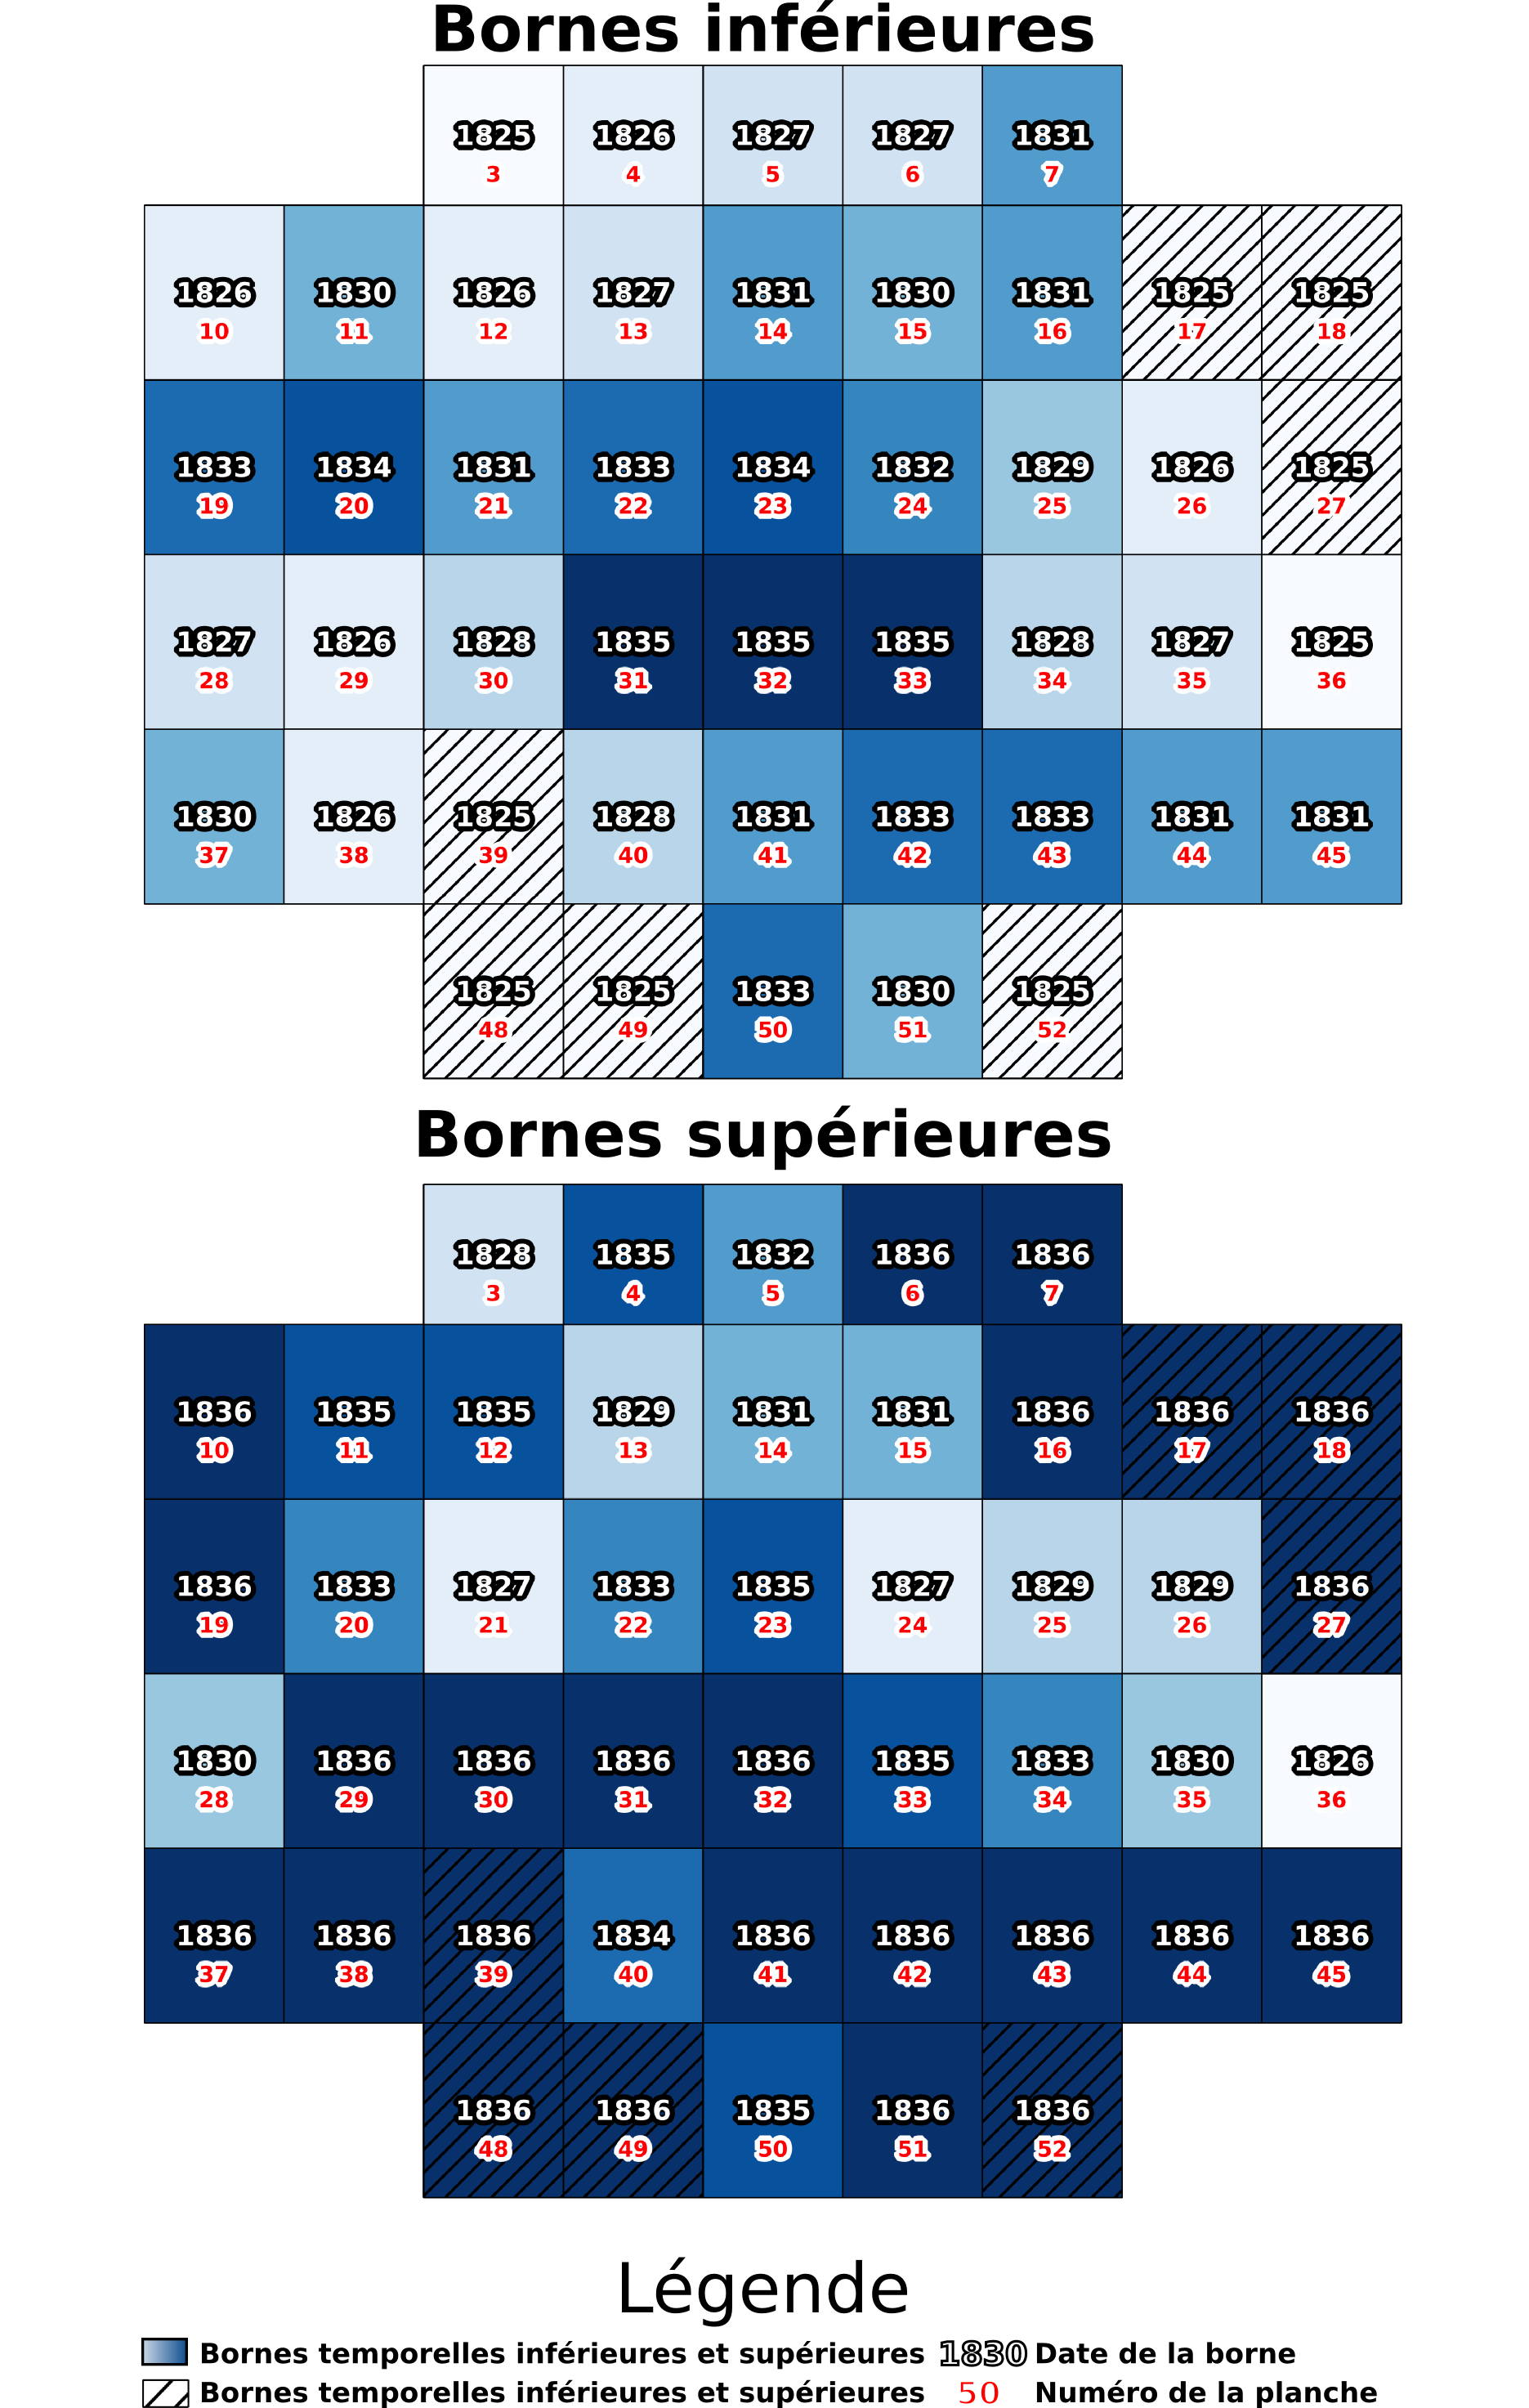
\includegraphics[width=0.8\textwidth]{bornes.png} 
\caption{Bornes temporelles inf�rieures et sup�rieures report�es sur l'emprise de chaque planche de l'atlas g�n�ral de Jacoubet.}
\label{figure:datation_jacoubet_fin_1}
 \end{figure}
\myparagraph{Cons�quences}
%\begin{wrapfigure}{r}{60mm}
\begin{figure}
	\centering
		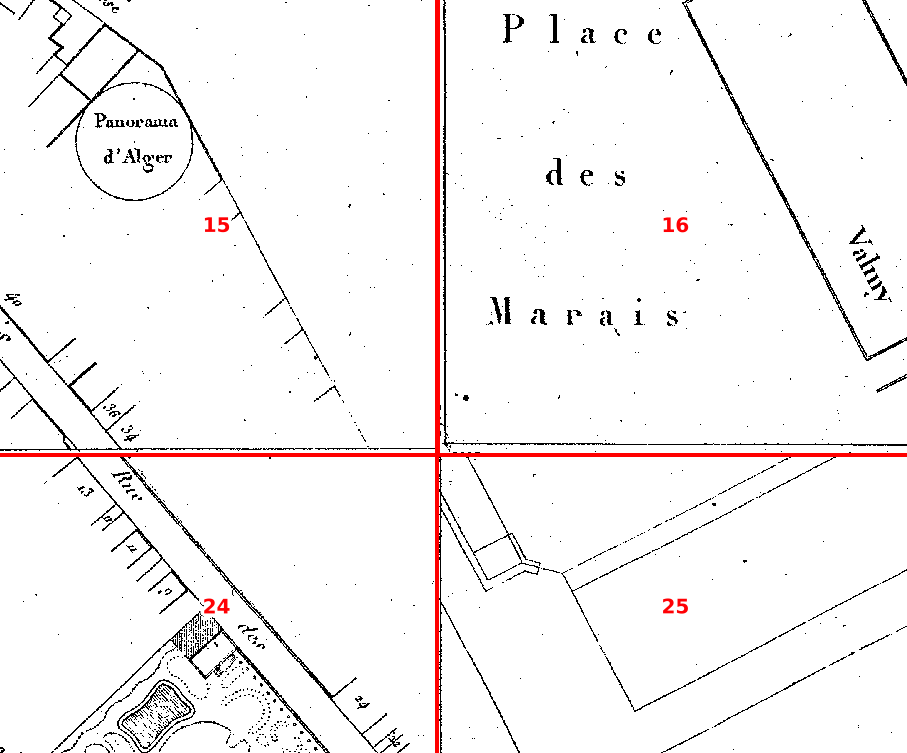
\includegraphics[width=0.4\textwidth]{incoherence_jacoubet.png}
	\caption{Un exemple d'incoh�rence entre quatre planches de l'atlas de Jacoubet, due � des p�riodes de dessin diff�rentes.}
	\label{figure:incoherence_jacoubet}
\end{figure}
%\end{wrapfigure}
La cons�quence premi�re de ces constatations est la remise en question totale de l'atlas de Jacoubet comme un objet homog�ne qui pourrait �tre trait� comme une repr�sentation globale et fiable de Paris en 1836.
Tout autant que les pr�c�dents plans, celui-ci n'est pas une ''tranche temporelle'' de Paris mais un mille-feuille qui accumule des fragments locaux d'une ville qui change sans cesse.
Plus encore, l'h�t�rog�n�it� des mises � jours entra�ne une d�coh�rence des diff�rentes parties du plan.
Ainsi, plusieurs feuilles de l'atlas pourtant adjacentes ne sont pas coh�rentes entre elles.
Un des exemples les plus parlants est illustr� dans la figure \ref{figure:incoherence_jacoubet}~: la place du Marais, qui contiendra � partir de 1833 l'entrep�t r�el des douanes\footnote{Ordonnance royale du 28 juin 1833.
Voir \cite{Guevel2004}}, pr�sente sur 4 planches de l'atlas, poss�de � chaque fois une repr�sentation diff�rente.
Dat�e de 1821 et entour�e de trois rues, elle est dans son �tat d'origine sur les planches 15 et 16, mais sur la planche 24 elle est absente.
Finalement, seule la planche 25 contient les trac�s de parties de l'entrep�t, construit � partir de 1833.
De telles incoh�rences se retrouvent r�guli�rement, en particulier dans les zones en pleine mutations au moment de la r�alisation du plan (en particulier les quartiers Saint-Lazare, Europe, Poissonni�re, Grenelle, canal Saint-Martin et Austerlitz).


\subsection{Jacoubet et l'administration parisienne~: l'insertion de l'atlas g�n�ral dans la gestion de la Ville}
\label{subsection:affairehourdequin}
%\myparagraph{Introduction}
Dans la section pr�c�dente, nous sommes parvenus � reconstituer la gen�se de l'atlas de Jacoubet, montrant ainsi qu'il s'agit d'un atlas particulier, non seulement en raison de son ambition et de ses dimensions, mais aussi par les liens que l'on voit se tisser entre l'atlas, son auteur et l'administration de la Seine.
Contrairement � la plupart des plans de l'�poque (la premi�re moiti� du XIX\up{e} si�cle voit en effet prolif�rer les plans de Paris, plus ou moins exacts), celui de Jacoubet a �t� r�alis� par un architecte qui travaillait � l'endroit m�me o� la voirie parisienne �tait administr�e.
�tant donn�e la pr�cision et l'�chelle du plan qui en font un concurrent s�rieux du cadastre de Vasserot et de l'atlas de Verniquet, on peut se demander si ce n'est pas ce plan qui a servi � la pr�fecture jusqu'� l'arriv�e de Haussmann, faisant de lui le ''plan officiel'' qui pr�c�de celui de Haussmann.
Dans ce cas, le plan de Jacoubet constituerait un des ''cha�nons manquants'' entre les plans de Vasserot et celui de Haussmann.
Ainsi, nous manipulerions -� part pour Maire- uniquement des plans qui ont servi � modeler la ville de Paris, t�moins privil�gi�s des projets et visions des administrateurs de la Seine.
\paragraph{}
Dans cette section, nous allons essayer de montrer que cet atlas n'est pas seulement une \oe uvre singuli�re, mais surtout qu'il est un r�v�lateur du fonctionnement de la pr�fecture de la Seine de 1820 � 1842 et qu'il ouvre une fen�tre sur une ville o� la fronti�re quasi-inexistante entre les fonctionnaires et les entrepreneurs priv�s profite largement aux int�r�ts des uns et des autres.
Nous allons �galement pouvoir donner quelques pistes permettant de comprendre comment il est possible que Jacoubet ait construit un atlas au 1/2.000\up{e}, sur une nouvelle triangulation, alors m�me qu'il travaillait � la pr�fecture.
\paragraph{}
Afin d'explorer cette hypoth�se, nous allons nous appuyer sur une affaire judiciaire datant de 1842, appel�e par ses contemporains \emph{Affaire Hourdequin}, dans laquelle une partie des employ�s de la pr�fecture charg�s de la r�alisation des plans d'alignements se sont vu accus�s de corruption et de vol de plans.
Cette affaire est devenue un v�ritable scandale lorsqu'elle a mis au jour la profonde corruption qui frappait les bureaux charg�s des alignements, pr�cipitant rapidement la plupart des responsables de ces bureaux, dont Th�odore Jacoubet, dans un proc�s qui durera 2 ans (18 novembre 1840-20 novembre 1842), demandera le t�moignage de 132 personnes et aura d'importantes r�percutions sur le fonctionnement de la pr�fecture et sur la r�organisation des services adopt�e plus tard par Haussmann.
\paragraph{}
Notre objectif n'est pas de d�rouler enti�rement le r�cit des 13 jours de proc�s, du 7 novembre au 20 novembre 1842, qui constituent le c{\oe}ur du scandale et pendant lesquels seront faites la quasi-totalit� des r�v�lations sur les bureaux de la pr�fecture.
Il s'agit plut�t d'en extraire les �l�ments qui nous permettront de reconstruire le contexte dans lequel le plan de Jacoubet a vu le jour, et d'entrevoir les raisons qui font de lui l'anc�tre des plans officiels de Paris.

\myparagraph{Le bureau des plans de Paris}
Afin de bien comprendre les relations entre les diff�rents personnages de l'affaire, mais aussi le statut de Th�odore Jacoubet au sein de la pr�fecture de la Seine, il faut savoir comment �taient organis�s les services g�rant la pr�paration et la r�alisation des plans d'alignements et de percements, ainsi que ceux qui avaient pour charge l'application des amendes pour non respect des r�glementations de voirie.
Comme nous l'avons dit, l'affaire Hourdequin va causer une totale r�organisation des bureaux de la pr�fecture.
Nous nous int�ressons donc ici uniquement � la p�riode qui pr�c�de, de 1823 - date d'arriv�e de Jacoubet- � 1842.
\paragraph{}
La figure \ref{fig:orga_plans} donne les diff�rentes organisations de la Grande Voirie de Paris, depuis le rattachement du bureau des plans jusqu'� la r�organisation de Haussmann.
Un \emph{bureau} est une unit� administrative qui correspond aujourd'hui � un \emph{service}; compos� d'un chef, d'un sous-chef et d'un nombre variable d'employ�s, il se voit charg� d'une t�che pr�cise.
Ainsi, le \emph{bureau des plans} a en charge la cr�ation des plans d'alignements de Paris, leur communication au public, au pr�fet et au conseil municipal, ainsi que la cr�ation de tout plan n�cessaire � l'�tablissement d'amendes, d'expropriations, etc.
C'est enfin ce bureau qui se voit charg� par Chabrol de la confection du grand plan de Paris en 48 parties.
Notons �galement que jusqu'en 1831, le bureau des plans �tait une annexe de la Grande Voirie et non directement une de ses composante, ce statut lui conf�rant une relative autonomie.
\paragraph{}
C'est dans ce bureau que Jacoubet entre en 1823 et b�tira toute sa carri�re sous les ordres de Chabrol puis de Rambuteau, son statut �voluant en fonction des �v�nements.
Ainsi, entr� comme simple architecte en 1823, il deviendra sous-chef adjoint en 1827, puis sous-chef en 1833.
Il finira par devenir chef du bureau en 1839 avant de redevenir sous-chef en 1842.
Il est de plus \emph{v�rificateur} depuis 1827, ce qui signifie qu'il contr�le, v�rifie les plans r�alis�s par les employ�s.
Sans son visa et sa signature, le travail est rejet�.
Jacoubet n'est donc pas un simple employ�, mais il joue un r�le important dans ce service alors qu'au m�me moment para�t son atlas.
\begin{figure}
 \centering
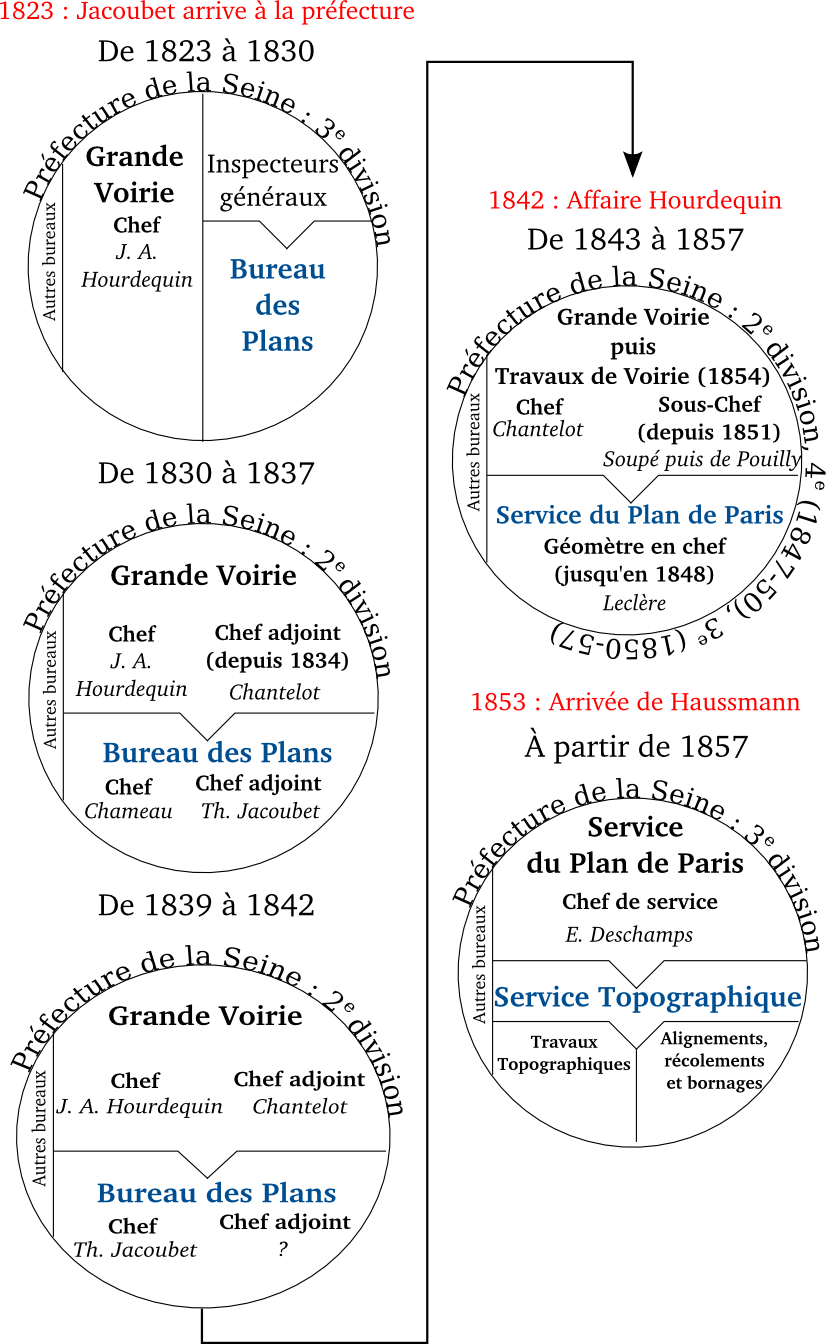
\includegraphics[width=0.8\textwidth]{org_bureau-plans.png} 
	\caption{Organisation du Bureau des Plans de Paris, depuis son d�placement du minist�re de l'int�rieur � la pr�fecture de la Seine jusqu'� sa r�organisation compl�te par Haussmann.
Chaque ligne rouge indique une phase de r�organisation majeure, ayant des cons�quences sur la production et l'utilisation des plans de Paris � la pr�fecture.
Les couleurs indiquent la filiation du bureau des plans.}
	\label{fig:orga_plans}
\end{figure}
Nous avons dit que l'affaire Hourdequin permettait de replacer l'atlas de Jacoubet dans le contexte de la pr�fecture de la Seine, mais aussi plus largement dans celui des pratiques des ing�nieurs cartographes de Paris durant la p�riode pr�c�dant Haussmann.
Pour reconstituer la matrice qui a permis la cr�ation de cet atlas, nous r�sumons le \emph{proc�s Hourdequin}.

\myparagraph{Les causes de l'affaire}
Le scandale du bureau des plans �clate le 18 novembre 1840 lorsque l'architecte Adolphe Morin, attach� au Cercle du Jeu de Paume du passage Sandri�, est arr�t� pour avoir d�rob� un billet de 1000 francs � un certain Nanteuil.
Arr�t�, l'enqu�te men�e sur ses ant�c�dents fait rapidement surgir plusieurs faits �tranges~: ancien employ� du bureau des plans � la pr�fecture de la Seine, il a �t� limog� en 1834 pour soustraction de plans\footnote{c'est � dire vol ou recel de feuilles ou minutes des plans produits � la pr�fecture.} et imitation des signatures de Auguste-Jean Hourdequin et Th�odore Jacoubet, respectivement chef de la Grande Voirie et sous-chef du bureau des plans.
Sur ces r�v�lations, la cour d'assises de la Seine nommera une commission dirig�e par H�ricart de Thury charg�e d'enqu�ter sur le bureau du plan.
Pendant un an les experts de la commission v�rifieront plus de 8000 pi�ces (plans, lettres, etc.), d�couvrant alors que de nombreux plans sont manquants, et que certains employ�s sont manifestement corrompus.
En cons�quence, le juge d�cide le 2 juillet 1842 de la mise en examen de 5 employ�s de la Grande Voirie pour les motifs suivants~:
\begin{itemize}
 \item Alexandre Philidor (employ�)~: Accus� d'avoir soustrait des plans servant � mettre en place une contravention, rendant celle-ci inapplicable, et d'avoir re�u un ''pot-de-vin'' de la part du contrevenant.
\item Nicolas Boutet (employ�)~: Accus� d'avoir d�truit des contraventions, ou d�lib�r�ment ralenti leur application en �change de dons en nature ou en argent.
\item Auguste-Jean Hourdequin~: Accus� d'avoir abus� de sa position pour sp�culer � son avantage sur des terrains et des propri�t�s menac�s de d�molition pour percement ou reculement, d'avoir favoris� certains entrepreneurs lors d'appels d'offres publics et enfin d'avoir accept� des dons d'argent en �change de la disparition de contraventions.
\item �tienne-Alexandre Solet~: Accus� de la soustraction de 5 plans, dont celui, officiel, d'une rue \emph{projet�e du Louvre � la Bastille}\footnote{Il s'agit sans nul doute du projet de la rue Imp�riale, pr�vue d�s le premier Empire, qui devait relier la place du Louvre � celle de la Bastille.
Jamais r�alis�, le projet sera finalement abandonn� au profit du percement de la rue de Rivoli.}
\item Adolphe Morin~: Accus� de faux en 1832 et 1834 et de la soustraction des plans-minutes\footnote{Le plan-minute d'un alignement ou de toute autre op�ration de voirie est un document sensible, puisqu'il est fait tr�s en amont de son ex�cution et de sa publicit� par ordonnance ou d�cret.} de la rue de la Verrerie et d'un terrain \emph{compris entre le Quai d'Orsay, les avenues de Suffren et de Lowendal, et le boulevard ext�rieur.}, ainsi que du plan officiel de la rue des Lombards.
\end{itemize}
Jacoubet n'est pas accus�, bien qu'il soit plac� momentan�ment en pr�vention \emph{pour n�gligences}.
Il compara�tra cependant r�guli�rement en qualit� de t�moin et d'expert cartographe, puis il prendra activement part aux d�bats et r�pondra dans une lettre ouverte aux attaques de l'avocat Gustave Louis Chaix d'Est-Ange \citep{JacoubetReponseEstAnge1842}.
Plut�t que de nous attarder sur chaque personnage, nous allons passer en revue les �l�ments d'accusation qui forment le canevas de l'entreprise de Jacoubet.
Ces �l�ments, au nombre de 3, ne font pas n�cessairement partie des faits incrimin�s lors du proc�s, soit parce qu'ils sont anciens, le tribunal d�cidant alors de les ignorer, soit parce qu'il s'agit d'accusations morales que la justice ne saurait traiter.
Il s'agit des �l�ments suivants, qui feront l'objet de points d�taill�s car ils permettent de mieux comprendre le r�le jou� par Jacoubet:
\begin{itemize}
 \item Les travaux personnels effectu�s par les agents du bureau sur leur temps de travail, et l'utilisation de pr�te-noms pour le financement de ceux-ci.
 \item Le vol de plans, la redondance de travaux (parfois faits par la m�me personne).
 \item Les actions sp�culatives men�es en association avec des entrepreneurs priv�s.
\end{itemize}

\myparagraph{Les travaux priv�s au sein du bureau des plans de Paris.}
Jusqu'en 1831, il existait trois groupes d'employ�s.
Les premiers, dont Jacoubet fait partie, �taient des salari�s � plein temps percevant un appointement.
Les seconds �taient attach�s temporairement au bureau et recevaient �galement un salaire fixe.
Enfin, les derniers �taient pay�s � la t�che.
Bien que les postes fixes offrent une plus grande s�curit�, ils pr�sentent l'inconv�nient de g�ner les travaux priv�s d'employ�s qui exercent �galement en parall�le un m�tier d'architecte ou de g�om�tre puisqu'il leur est interdit d'y travailler pendant les heures dues � la pr�fecture.
Ainsi donc, la pratique courante \citep[p.2-3]{GazetteTribunaux18421107} consistait � s'entendre avec les employ�s pay�s � la t�che, qui servaient de pr�te-noms.
Tol�r�e pendant un temps, cette pratique sera massivement utilis�e par Jacoubet pour r�aliser son atlas.
En effet, il appara�t dans le cours du proc�s que l'accus� Solet, qui jusqu'en 1832 sera dessinateur pour le bureau des plans, avait pr�t� son nom pour certaines t�ches r�alis�es en fait par Jacoubet.
En particulier, il a travaill� comme dessinateur sur l'atlas au moins jusqu'en 1829 et dessinera, d'apr�s Jacoubet, pr�s des deux tiers du plan \citep{GazetteTribunaux18421111} qu'il effectuera dans son atelier priv� et non � l'H�tel de Ville.
\\
Jacoubet, dans son t�moignage le 11 novembre 1842~\citep{GazetteTribunaux18421111}, annonce ainsi qu'il a fait travailler sur son plan deux personnes ext�rieures � la pr�fecture, dont on ne conna�t pas les noms, recrut�es pour l'occasion, ainsi que deux employ�s~: Solet et un ing�nieur civil nomm� Cannot-Tissier.
Ces pratiques, si elles semblent tol�r�es par Chabrol, vont dispara�tre en 1831 sous la direction du pr�fet de Bondy.
Celui-ci, pour faire stopper ces agissements qui nuisent grandement � la r�alisation du grand plan voulu par Chabrol, nomme en 1831 Hourdequin � la t�te de la Grande Voirie, lequel s'empresse d'interdire le d�marrage de nouveaux travaux priv�s, mais il autorise la poursuite de ceux en cours.
Un t�moignage de l'accus� Morin indique d'ailleurs que Jacoubet a continu� � utiliser cette pratique apr�s 1830.
Si la fiabilit� des propos de Morin, renvoy� de la pr�fecture par Jacoubet en 1834, est presque nulle, il est tout de m�me possible que Jacoubet a continu� a faire dessiner son plan puisqu'il �tait d�j� en cours et r�alis� \emph{sous les bonnes auspices} de l'ancien pr�fet.


\myparagraph{La soustraction de plans ou l'�chec du projet de Chabrol.}
Le projet de grand plan de Paris, initi� par Chabrol en 1824, avait rapidement �t� divis� en 48 parties pour acc�l�rer sa r�alisation.
Chacune des 48 parties avait �t� subdivis�e en 24 plus petites, un nombre variable de ces parties, au 1/144\up{�me}\footnote{Il s'agit de la m�me �chelle que les plans des rues de Verniquet, signifiant peut-�tre qu'il s'agissait d'une mise � jour de ces plans, dans le but de suivre le m�me proc�d� que celui qui avait �t� adopt� en 1783} �tant alors assign� � chaque membre du bureau des plans.
Sur le m�me mod�le que les cadastres de Vasserot, Chabrol avait ajout� un niveau entre le grand plan et ceux des rues.
Ainsi, un plan d'ensemble de chacune des 48 parties devait �tre r�alis� en parall�le des plans des rues.
\paragraph{}
Les ordres de Chabrol ne sont suivis d'aucun effet puisque, le 12 juillet 1833, le nouveau pr�fet Rambuteau, constatant que le plan est � peine commenc�, cr�e le poste de \emph{chef de bureau des plans} qui se voit charg� de faire ex�cuter le plan et de r�partir les cr�dits allou�s au bureau dans ce but.
Pourtant, cette mesure n'a aucun effet~: si l'atlas de Jacoubet progresse � grands pas, le plan officiel de l'H�tel de Ville reste au point mort.
Plusieurs t�moins de la pr�fecture rapporteront que le bureau des plans se trouvait alors \emph{dans un �tat de d�sordre tel} que tous les travaux men�s �taient inutilisables ou jamais effectu�s~\citep{GazetteTribunaux18421108}.
On peut cerner quelques unes des causes de ce d�sordre.
\paragraph{}
Premi�rement, le travail � la t�che encourage largement les g�om�tres et dessinateurs � privil�gier la quantit� sur la qualit�.
Les plans sont alors inexacts, incomplets ou faux, voire produits plusieurs fois.
Le bureau met en place tr�s t�t (peut-�tre d�s 1823) un syst�me de v�rification cens� emp�cher ces malfa�ons.
Ainsi, lorsqu'un employ� r�alise un travail, il le pr�sente � deux agents v�rificateurs qui le contr�lent et, s'il est correct, le signent.
Il suffit ensuite d'aller voir le responsable des paiements pour obtenir son d� en �change du plan.
En 1827, Jacoubet devient v�rificateur en m�me temps que sous-chef, rejoint quelques ann�es apr�s par Hourdequin.
Nul plan ne peut �tre pay� sans leurs accords.
Si ce syst�me semble efficace, il �chouera tout de m�me~: en 1832, Morin imitera les signatures de Jacoubet et Hourdequin obtiendra un paiement de 1512 francs.
Il ne sera d�masqu� qu'en 1834 lorsqu'il tentera de nouveau d'obtenir paiement d'un travail d�j� effectu� pour la somme de 1883 francs.
\paragraph{}
Deuxi�mement, plusieurs employ�s (Solet, Morin et Boutet) emportent chez eux plusieurs plans entre 1833 et 1838.
Arguant qu'ils leurs servent � dessiner le plan d'alignement, certains les conserveront m�me apr�s leur d�part de la pr�fecture.
Ainsi Solet, qui d�missionne en 1836, conservera les plans du Champs de Mars, de la rue de la Verrerie et des Lombards que les enqu�teurs retrouveront � son domicile en 1842.
Les soustractions sont telles qu'entre 1823 et 1841, dates de deux inventaires des plans poss�d�s par le bureau \footnote{Un troisi�me est fait en 1834, mais les enqu�teurs le jugent inutilisable car tr�s incomplet}, plus de 500 plans - soit plus de 4\% du total des plans poss�d�s- disparaissent.
\\
Le travail est si inefficace qu'en 1841, un seul 48\up{�me} du plan g�n�ral d'alignements est termin�, montr� lors du proc�s sous la forme d'un \emph{grand plan de 6 pieds carr�s}\footnote{Soit environ 2 m�tres carr�s.} sur lequel sont trac�s en jaune tous les projets d'alignements et de percements.
\\
On peut se demander alors quel statut occupe l'atlas de Jacoubet, qui est alors le seul plan d�taill� et g�n�ral de Paris, le plan en 48 parties �tant un �chec.
La r�ponse est donn�e par Jacoubet lui m�me, qui dans son interrogatoire pr�cise que son plan �tait utilis� par les employ�s du bureau qui en faisaient des calques.
Cela signifie que, pour r�aliser les plans de chacune des 48 parties, les dessinateurs prenaient appui sur le trac� de l'atlas de Jacoubet.
Celui-ci se justifie d'ailleurs d'avoir employ� le personnel de la pr�fecture pour son propre atlas en invoquant l'utilit� qu'il avait pour elle.
Ainsi, bien que le l'atlas g�n�ral n'ait jamais eu le titre de plan officiel, il sera de fait utilis� comme tel par le bureau des plans de Paris.
Finalement, Jacoubet sera parvenu � la fois � faire de son travail une r�f�rence dans la sph�re des g�ographes priv�s, mais �galement au sein m�me de l'H�tel de Ville.

\myparagraph{Le bureau des plans et la sp�culation immobili�re}
Le dernier point du proc�s sur lequel nous allons nous attarder est celui des relations entretenues par certains employ�s de la pr�fecture et des entrepreneurs et agents d'affaires priv�s.
L'essentiel des op�rations sp�culatives men�es au sein du bureau des plans reposent sur une m�canique simple.
En effet, lorsqu'un projet d'alignement ou de percement doit mener � la destruction de maisons et au retranchement de terrains, la Ville rach�te ces terrains � l'issue de n�gociations avec chaque propri�taire.
Le plus souvent, la transaction est tr�s avantageuse pour le propri�taire. Bien conscient des enjeux, celui-ci revend le terrain � un prix sup�rieur � sa valeur r�elle.
Si le terrain est construit, il peut �galement obtenir le droit de revendre les mat�riaux issus de la d�molition.
Pour se pr�munir d'une trop forte sp�culation sur les terrains, la pr�fecture ne publie les plans d'expropriation que peu de temps avant le d�but des n�gociations et des travaux.
De plus, ces plans ne sont pas diffus�s publiquement mais consultables par les propri�taires au bureau des plans.
Il s'agit alors pour les employ�s du bureau des plans, qui sont inform�s avant le grand public des diff�rents projets, d'acheter � bas prix aux propri�taires ignorants les diff�rents terrains expropri�s ou recul�s, puis de revendre ces m�mes terrains � la pr�fecture � l'aide de pr�te-noms conciliants ou int�ress�s.
\paragraph{}
Il s'agit cependant d'actes isol�s, et non d'une corruption qui atteindrait l'ensemble de la pr�fecture.
En particulier, nous nous attarderons sur les agissements de Hourdequin, alors chef de la Grande Voirie de Paris, � l'origine en 1843 d'une r�organisation du bureau des plans annonciatrice des changements adopt�s par Haussmann 10 ans plus tard.
Sur les 13 faits de corruption reproch�s au chef de la Grande Voirie, 9 seront effectivement retenus\citep[pp. 3-4]{GazetteTribunaux18421107}.
Nous ne rapporterons ici que les 3 plus importants d'entre eux, qui suffisent � donner un aper�u r�v�lateur du fonctionnement d'un des organes les plus importants de la pr�fecture de la Seine.
\paragraph{}
La premi�re affaire renseigne sur la relation entretenue par Hourdequin avec l'entrepreneur en travaux publics Dubrugeaud dans un objectif d'enrichissement personnel.
En juillet 1836, le conseil municipal adopte le projet de la rue d'Arcole qui devait �tre cr��e gr�ce � l'alignement des rues Chevet Saint-Landry et Saint-Pierre aux B{\oe}ufs.
La concession est donn�e � l'entrepreneur Dubrugeaud, qui se voit allouer la somme de 460.000 francs -pay�e apr�s travaux- pour l'ensemble des op�rations ainsi que le droit de revente des mat�riaux issus de la d�molition, � la condition que les travaux soient r�alis�s en un an seulement.
Termin� dans les temps, le percement de la rue d'Arcole permet � Dubrugeaud de d�gager un b�n�fice de 279 204 francs gr�ce � la vente des mat�riaux et � plusieurs op�rations de sp�culation immobili�re dans la rue voisine de Constantine.
L'extr�me rentabilit� de cette op�ration n'aura �t� pourtant possible que gr�ce � Hourdequin, alors associ� de l'entrepreneur.
Sur la rue d'Arcole elle-m�me, le tribunal ne rel�vera que le z�le �tonnant avec lequel il soutiendra la candidature de Dubrugeaud, puis un acompte de 10.000 francs qui permettront de terminer les travaux � temps.
Surtout, les op�rations men�es sur l'�le de la Cit� seront l'occasion pour eux d'acheter plusieurs propri�t�s dans la future rue de Constantine avant m�me que le projet ne soit rendu public.
Ignorant la d�molition future de leurs maisons, plusieurs propri�taires les vendirent � bas prix � l'entrepreneur qui, inform� des alignements et d�molitions pr�vus par Hourdequin, pu les revendre � la ville avec une marge importante.
En remerciement des services rendus par Hourdequin, son associ� lui offrira finalement la somme de 17.000 francs.
\paragraph{}
La seconde affaire d�voile une corruption encore plus flagrante.
En 1840, le baron Millin de Grandmaison, propri�taire de plusieurs immeubles sur la place de la Madeleine, avait pr�vu d'aligner ceux-ci, mais �galement de faire percer une nouvelle rue entre la place et la rue d'Anjou dans le but de revendre les terrains ainsi d�gag�s.
Il soumet alors le projet au conseil municipal, ajoutant �galement l'abandon d'une maison d'une valeur de 40.000 francs se trouvant sur le trac� de la rue, en �change de l'aquisition d'une maison situ�e au \no16 rue de la Madeleine appartenant � la Ville et de la remise d'une soulte de 150.000 francs\footnote{Dans un contrat d'�change, la soulte d�signe une somme d'argent qu'une des partie remet � l'autre pour compenser un d�s�quilibre entre la valeur des objets �chang�s.}.
Le conseil municipal puis le pr�fet refusant de c�der plus de 100.000 francs\footnote{Une note du pr�fet Rambuteau le 7 juin 1841 indique ainsi~: \emph{Borner � 100 000 francs; et s'il s'y refuse, ajourner l'affaire}}, le dossier reste bloqu� � la pr�fecture jusqu'� ce que M. de Grandmaison ne prenne contact avec Hourdequin.
Gr�ce � un rapport �logieux remis au conseil municipal le 28 juillet 1841, ce dernier obtient l'accord de la Ville pour une somme r�duite � 125.000 francs et r�clame � Grandmaison la somme de 25.000 francs pour ses bons services.
La lettre suivante, dat� du 20 juin 1841, t�moigne de l'accord entre eux~: 
\\
\emph{Je vous envoie ma demande au pr�fet , mon cher Hourdequin, en vous priant de vous occuper de suite de cette affaire; je prends l'engagement, si l'on m'accorde les 125 000 francs de soulte que je demande, de vous remettre sur cette somme 25 000 francs. Tout � vous d'amiti�. Sign�~: baron de Grandmaison.}
\paragraph{}
Le dernier exemple donne cette fois un aper�u d'actes de sp�culation orchestr�s directement par Hourdequin et rendus possibles par sa situation � la pr�fecture.
Ainsi en 1833 il existait un projet d'allongement de la rue de l'Aiguillerie (aujourd'hui remplac�e par la partie de la rue des Lombards entre la rue Sainte-Opportune et la rue Saint-Denis) jusqu'� la rue des Fourreurs (aujourd'hui rue des Halles).
Connaissant le projet � l'avance, Hourdequin ach�te en ao�t 1834 pour 36.100 francs la propri�t� situ�e au \no6 rue des Fourreurs\footnote{Il s'agit d'une propri�t� ayant issue \emph{sur l'une et sur l'autre}.
Ici le cadastre de Vasserot et l'atlas de Jacoubet se contredisent, la seule maison correspondant � la description, correctement num�rot�e sur Vasserot, est num�rot�e 8 sur l'atlas g�n�ral.} sous le nom de \emph{Laurent Huet}.
Le 12 f�vrier 1835, Hourdequin -sous le nom de Huet- et son voisin poss�dant les maisons 14 et 22 rue des Fourreurs \footnote{Le \no22, visible sur Vasserot, correspond � la maison dont l'issue est sur la rue de l'Aiguillerie, oppos�e � celle de Hourdequin.
Le num�ro 14 n'est pas indiqu�, et se trouve � l'oppos� de la rue sur Vasserot.}, soumettent tous deux l'achat de leurs maisons � la Ville.
Cette fois, le chef de la Grande Voirie use de sa position officielle et appuie fortement les deux demandes qui se trouvent accept�es par le conseil municipal d�s le 6 mars 1835.
La vente est consentie le 8 mai et finalement les maisons sont vendues le 4 septembre.
Ainsi, les deux propri�taires auront atteint leurs objectifs en moins d'un an.
La vente de la maison et des mat�riaux rapporteront 48.274 francs, formant donc un b�n�fice de 12.174 francs.
Son voisin, nomm� Cady, obtiendra 80.000 francs pour la vente de sa maison, et 6.000 francs pour les mat�riaux.
En remerciement, il versera 10.000 francs � Hourdequin.
\paragraph{}
Ainsi donc, Hourdequin profitera sa situation privil�gi�e � l'H�tel de Ville pour s'associer avec divers acteurs priv�s, agents d'affaires mais aussi simples propri�taires profitant de l'occasion.
Des trois affaires pr�sent�es, il retirera un b�n�fice de 64.174 francs dont plus de 80\% seront form�s de ''pots-de-vins''.
Pourtant, le jury ne le d�clarera coupable que de l'op�ration men�e avec Millin de Grandmaison, jugeant la plupart des autres affaires \emph{peu morales} mais toutefois l�gales.
Quant � Jacoubet, il appara�t totalement �tranger aux diverses corruptions qui agitent le bureau des plans, bien qu'il connaisse plusieurs agents d'affaires m�l�s au scandale \footnote{Notamment Denis-Laurent-Aubin Jaloureau, agent d'affaire de Hourdequin.}.
Pourtant, lorsque Eug�ne Deschamps, conservateur du plan et futur chef du service des plans sous Haussmann, est interrog� par le procureur sur l'�ventuelle utilit� de l'atlas de Jacoubet -qui indique tous les projets de voirie- pour les sp�culateurs parisien, celui-ci r�pondra~: \emph{Du jour o� l'administration a autoris� un pareil plan, les sp�culateurs ont pu avoir tous les renseignements possibles sans venir � nos bureaux. Cet Atlas leur offre m�me des renseignements plus complets, puisqu'il contient le plan de tous les �lots r�unis}.
\\
Si Jacoubet semble s'�tre tenu � l'�cart de ces pratiques, il aura tout du moins cr�� un outil dont l'utilit� pour les sp�culateurs immobiliers ne semble pas avoir �chapp� au tribunal.

\subsection{Notes et remarques}
\myparagraph{Sur l'atlas G�n�ral de Jacoubet et son devenir au bureau des plans}
Si l'{\oe}uvre de Jacoubet n'atteindra jamais la renomm�e de l'atlas de Verniquet, il n'en restera pas moins l'un des plans les plus importants de la premi�re moiti� du XIX\up{e} si�cle pour sa pr�cision et sa richesse d'informations.
Il permettra � son auteur de remporter la m�daille d'argent � l'exposition des produits de l'industrie fran�aise en 1834, de se voir proposer une place � la chambre des Pairs et finalement d'obtenir une telle notori�t� publique qu'il deviendra un expert reconnu de la topographie parisienne.
\paragraph{}
Il est difficile de savoir si l'atlas a �t� largement utilis� par la pr�fecture de la Seine.
En effet, si un plan d'alignements du quartier des Halles dat� de 1848 est bas� sur l'atlas de Jacoubet - il en est d'ailleurs un des auteurs -, rien ne permet d'affirmer qu'il soit directement li� � la Grande Voirie.
En effet, le projet de r�organisation des Halles avait alors fait na�tre divers projets �manant d'architectes et g�ographes priv�s.
En novembre 1842, le chef de la division de la Voirie Planson annonce que le plan de Chabrol, dont seul un quarante-huiti�me �tait fait en 1841, avait �t� \emph{repris avec ardeur} en juillet 1842 et qu'il �tait d�sormais \emph{fort avanc�}.
Cependant, lorsque Haussmann lancera la production du nouveau plan de Paris en 1856, la pr�fecture ne semble pas disposer d'un plan d'ensemble de Paris.
Sans doute la r�alisation du plan g�n�ral annonc�e par Planson n'�tait-elle pas aussi rapide qu'il le souhaitait.
\paragraph{}
De plus, le plan de Verniquet avait �t� utilis� par les services officiels au d�but du XIX\up{e} si�cle car aucun autre plan n'�tait aussi g�om�triquement exact.
Au contraire, lorsque Jacoubet publie son atlas le cadastre parisien est en grande partie termin�, le plan en 48 quartiers de Vasserot a �t� fini en 1821, celui par �lots est bien avanc� et les plans des maisons seront termin�es en 1836.
Ainsi l'atlas n'est-il pas le seul plan g�n�ral en lice.
Les plans de percements des rues contemporains de l'atlas de Jacoubet sont d'ailleurs trac�s sur le plan parcellaire de Vasserot, bien plus adapt� � des op�rations impliquant expropriations et reculements.
Jacoubet n'atteindra donc qu'en partie son objectif~: si son atlas est un vrai produit de l'administration de la Seine, sans laquelle il n'aurait jamais pu voir le jour, il ne sera jamais adopt� officiellement par la pr�fecture, et s'il a aid� � la cr�ation du plan de Chabrol il ne semble ne l'avoir jamais remplac�.

\myparagraph{Sur le bureau des plans}
Au travers de l'affaire Hourdequin, nous avons pu avoir un aper�u des dysfonctionnement des services officiels destin�s � g�rer la voirie parisienne.
Cependant la corruption � l'{\oe}uvre au bureau des plans n'y est pas circonscrite et d'autres affaires �clabousseront la pr�fecture.
Ainsi le 7 d�cembre 1843, Tr�mery, ing�nieur des Ponts-et-Chauss�es et inspecteur g�n�ral des carri�res sous la Seine est contraint � la d�mission lorsque la justice d�couvre l'existence de 16 employ�s fictifs suppos�s travailler dans les carri�res et dont les salaires sont d�tourn�s pour l'enrichissement personnel des dirigeants des carri�res\footnote{En plus de Tr�mery, le chef Poirier-Saint-Brice sera plac� en retraite.}.
Pourtant la justice se montrera �tonnamment cl�mente~: Tr�mery ne sera jamais poursuivi.
Quant aux protagonistes de l'affaire Hourdequin seuls trois d'entre eux seront condamn�s, Solet et Boutet �tant acquitt�s.
Si Hourdequin et Philidor se voient sanctionn�s de quatre et trois ans de prison pour corruption, la plupart des faits de corruption pourtant jug�s vrais par le tribunal ne seront pas retenus.
Ainsi, sur neuf faits qui lui sont imput�s, Hourdequin ne se verra condamn� que pour ses rapports avec Millin de Grandmaison.
Quant � Morin, il sera finalement puni de trois ans de prison pour faux et usage de faux.
Pour tous les accus�s, le jury ne consid�rera pas la soustraction de plans.
Pour conclure sur l'affaire Hourdequin, laissons le mot de la fin au journaliste de la \emph{Gazette des Tribunaux} qui nous a permis de retracer l'histoire du plan de Jacoubet~:
\paragraph{}
\emph{Nous n'avons pas � nous expliquer sur la d�cision qui vient d'�tre rendue}  (Le jugement final du 19 novembre 1842).
\emph{Mais il y a dans ce proc�s une autre question que celle soumise au jury, et il ne faut pas que tout se termine avec son verdict. Nous ne voulons rien exag�rer, rien amoindrir; nous ne voulons pas rechercher si les condamn�s sont les seuls coupables, ou s'il n'en manquait pas d'autres � c�t� d'eux sur les bancs de la Cour d'assises~: ce sont l� des questions qu'il ne nous appartient pas de r�soudre, mais que les r�v�lations du d�bat commandent � la justice d'�tudier s�rieusement.\vspace{11pt}
\[...\] Un tel �tat de chose appelle � un rem�de �nergique et prompt~: il faut que l'opinion publique soit rassur�e; il faut que l'administration elle-m�me soit mise � l'abri de cette esp�ce de suspicion l�gitime sous le coup de laquelle elle est plac�e. Car, c'est l� une des tendances de l'opinion, d'exag�rer le mal et de le g�n�raliser.\vspace{11pt}
Sans doute de telles questions sont graves et difficiles. Mais sans toucher imprudemment � l'ensemble du m�canisme administratif, on peut se demander si le contr�le et la surveillance sont ce qu'ils doivent �tre; si les garanties de savoir et de moralit� sont toujours s�rieusement consult�es � l'entr�e de chacun dans la carri�re administrative; si enfin la question des salaires est tranch�e de fa�on � placer le fonctionnaire au-dessus du besoin et de la corruption, ou si au contraire elle n'est pas domin�e par ce besoin de cr�er incessamment des emplois inutiles et de pourvoir aux n�cessit�s de la faveur.}
\paragraph{}
Il semble que la Gazette ait �t� entendue puisque cette affaire causera la premi�re grande r�organisation de la voirie parisienne, pr�c�dant celle op�r�e par Haussmann quelques ann�es plus tard.
En effet, le pr�fet Rambuteau, apr�s avoir supprim� momentan�ment le bureau des plans, mettra en place une nouvelle hi�rarchie avec l'objectif clair d'emp�cher toute perte de plan et toute corruption.
Ainsi le bureau sera d�sormais soumis � l'autorit� directe de la Grande Voirie, divis� en quatre sections elles-m�mes plac�es sous l'autorit� d'un g�om�tre en chef.
Le poste de conservateur des plans, occup� depuis 1834 par Eug�ne Deschamps sera �galement profond�ment modifi�.
Ind�pendant des sections et plac� directement sous l'autorit� du g�om�tre en chef, le conservateur est d�sormais le gardien des plans d'alignements, dont l'acc�s n'est plus autoris� que sur d�rogation du pr�fet.
Cette organisation, visible dans la figure~\ref{fig:orga_plans}, restera la m�me jusqu'en 1857.

\myparagraph{Sur Jacoubet}
Jacoubet quant � lui continuera � �diter son atlas, d'abord en grand format puis sous sa forme r�duite au 1/10.000\up{e} et finalement l'�tendra dans ses nouvelles limites en 1860 \citep{MAPJacoubet1860}.
Nous ne savons pas s'il a conserv� son poste au bureau des plans apr�s la r�organisation de 1842 mais il est certain qu'il n'�tait plus � la pr�fecture apr�s 1852.
En effet, apr�s avoir particip� � la r�volution de 1848 et s'�tre oppos� au coup d'�tat de Napol�on III, il sera condamn� � l'exil � Londres le 7 mars 1852\footnote{On lit en effet dans La Presse du 7 mars 1852 qu'\emph{il vient d'�tre d�livr� des passeports aux personnes [] qui se sont engag�es � quitter Paris dans les 24 heures. Pour Londres : Jacoubet, architecte.}}.
Cette peine sera pourtant annul�e et il se verra intern�\footnote{Assign� � r�sidence} dans la propri�t� de sa famille � Montesquieu-Volvestre pr�s de Toulouse.
Pourtant, c'est sans h�sitation que le comte Sim�on fera appel � lui en 1853 lorsqu'il formera la commission des embellissements de Paris voulue par Napol�on III.
C'est en tant que cartographe et sp�cialiste de Paris que Sim�on louera Jacoubet dans une lettre qu'il adresse � Persigny le 2 septembre 1853 \citep{Casselle2000}.
Celle-ci renseigne d'ailleurs aussi bien que le proc�s sur un personnage dont le talent de commer�ant n'avait rien � envier � celui de cartographe~: non seulement Napol�on III \emph{conna�t Jacoubet}, pourtant r�publicain et condamn� � l'internement, mais surtout celui-ci tente de vendre � l'empereur la gravure de son plan pour chaque rue � percer pour 1200 francs par rue, soit 4800 francs au total \footnote{\emph{M. Jacoubet, architecte, charg� autrefois du bureau des plans de la ville, poss�de tous les �l�ments de ce travail. Il s'engagerait, moyennant un  prix � forfait de 1200 francs par rue � ouvrir, � fournir, en un mois, ces documens � la Commission. Pour quatre rues, ce serait une d�pense de 4800 francs, qu'il vous serait facile d'imputer sur les fonds du minist�re.}\citep{Casselle2000}}.


\myparagraph{Hypoth�se de travail }
On remarquera que dans l'ensemble de nos d�veloppements autour de l'atlas g�n�ral, nous n'avons jamais s�par� clairement les phases de lev� topographique des planches des phases de gravure.
� l'inverse m�me nous avons consid�r�, tout comme Jacoubet l'annonce en 1842, que les minutes de son atlas �taient termin�es en 1825.
Notre choix s'explique pour deux raisons.
\paragraph{}
D'abord, nous avons montr� que la version originale de l'atlas publi�e en 1836 comportait de nombreuses corrections effectu�es depuis la gravure des premi�res planches  en 1827.
Contrairement � l'atlas de Verniquet o� le plan a d'abord �t� enti�rement lev� puis grav� une fois termin�, cette fois ce processus a �t� appliqu� plusieurs fois sur des parties de l'atlas, � divers moments.
\paragraph{}
Ensuite, nous devons rappeler que la r�alisation de l'atlas de Jacoubet suit l'�dition de la version r�duite et mise au net du plan de Verniquet en 1825, puisque le prospectus annon�ant les premi�res livraisons date de 1826.
Nous avons �galement fait remarquer pr�c�demment que malgr� les conclusions du proc�s intent� par M\up{me} de Chavagnac � Jacoubet, il para�t difficile qu'un plan de l'ampleur de celui-ci ait �t� enti�rement lev� et dessin� par une seule personne (les quatre autres n'interviendront qu'apr�s 1825) en une ann�e.
Notons �galement que le tribunal conclura non pas que l'atlas est enti�rement nouveau, mais qu'il est suffisamment diff�rent du plan de 1825 par son contenu et sa triangulation pour �tre consid�r� comme une oeuvre originale, laissant ouverte l'hypoth�se d'une filiation entre les deux atlas.
\paragraph{}
Nous posons donc l'hypoth�se d'une filiation directe entre l'atlas g�n�ral et le plan de Verniquet.
En effet, la mise � jour du plan de Verniquet en 1825 a n�cessit� d'effectuer les relev�s topographiques relatifs au rajout des nouvelles rues et places de la ville.
Nous supposons donc que la triangulation effectu�e par Jacoubet n'est pas tout � fait nouvelle, mais compl�te celle plus ancienne de Verniquet.
Il utilisera en effet plusieurs fois d'autres plans pour compl�ter les informations de son atlas.
Par exemples, les b�timents en coupe qu'il repr�sente sont issus de l'atlas des 48 quartiers de Vasserot.
Si cette hypoth�se se v�rifie nous pourrons alors consid�rer l'atlas de Jacoubet comme l'h�ritier direct du plan de Verniquet pour le XIX\up{e} si�cle.
\newpage
\section{Conclusion}
Au cours de ce chapitre, nous avons pr�sent� les diff�rents plans que nous utilisons dans leur contexte, � la fois pour montrer les sp�cificit�s de chacun et pour donner l'intuition des liens de filiation les unissent, ainsi que pour identifier les temps valides de chacun.
En effet, il appara�t que ces diff�rents plans et atlas, pourtant d'origines et de formes tr�s vari�es, sont tous li�s les uns aux autres.
Ce lien peut �tre direct comme entre le plan de Maire, celui de Delagrive et l'atlas de Verniquet, ou encore entre celui des 48 quartiers de Vasserot et celui de Verniquet, o� les plans les plus anciens sont utilis�s comme fonds de cartes ou sont simplement mis � jour.
Il peut �tre �galement indirect, parce qu'un m�me contexte les lie ou que la r�alisation d'un plan d�coule de l'existence -ou plut�t de l'obsolescence- d'un autre, comme c'est le cas pour le plan de Haussmann avec celui de Jacoubet ou bien encore celui de Jacoubet avec Verniquet et Vasserot.
\paragraph{}
Lorsqu'elle est directe, la filiation entre deux plans est int�ressante � consid�rer pour leur utilisation au sein d'un SIG.
En particulier, les �l�ments suivants sont � consid�rer~:
\begin{itemize}
\item Lorsque deux plans sont li�s, les d�formations g�om�triques du premier peuvent �tre corr�l�es � celles du second.
D�s lors, il peut �tre pr�f�rable d'utiliser le premier comme r�f�rentiel pour r�f�rencer le second, plut�t qu'un r�f�rentiel absolu -souvent un plan r�cent-.
\item Un lien direct peut permettre d'expliquer d'�ventuelles incoh�rences dans le second plan, soit parce qu'il s'agit d'oublis, soit en raison du choix de son auteur (Maire par exemple figure des b�timents pourtant d�truits apr�s 1803).
\item Concernant le contenu des plans, un h�ritage direct entre deux plans indique une proximit� sur les sp�cifications de saisie des objets g�ographiques et leur repr�sentation cartographique lorsqu'ils sont communs (c'est par exemple le cas des b�timents de l'atlas de Jacoubet, provenant du plan des 48 quartiers de Vasserot).
Par cons�quent, les sp�cifications des donn�es extraites de ces plans par vectorisation doivent �galement �tre communes.
\end{itemize}
Lorsqu'elles sont indirectes, les filiations entre plans permettent de mieux comprendre les particularit�s d'un plan ou bien sa cr�ation.
C'est par exemple le cas de l'atlas de Jacoubet qui n'aurait sans doute pas vu le jour sans l'absence de mise en place d'un rempla�ant du plan de Verniquet par la pr�fecture.
la puissance financi�re
Au travers de ce chapitre, nous avons ainsi recompos� les filiations, r�sum�es dans la figure \ref{fig:filiations}.
On voit donc que les plans sont largement li�s entre eux, en particulier jusqu'au milieu du XIX\up{e} si�cle et qu'ils sont majoritairement affili�s � l'atlas de Verniquet.
De plus, en cent ans, seules deux nouvelles triangulations v�ritables ont �t� effectu�es, si l'on consid�re que celle de Jacoubet est au mieux partielle.
Ceci renseigne d'autant plus sur le caract�re exceptionnel du travail de Verniquet~: la seule triangulation qui suivra sera l'{\oe}uvre d'un service entier de la pr�fecture de la Seine.
\begin{figure}
	\centering
		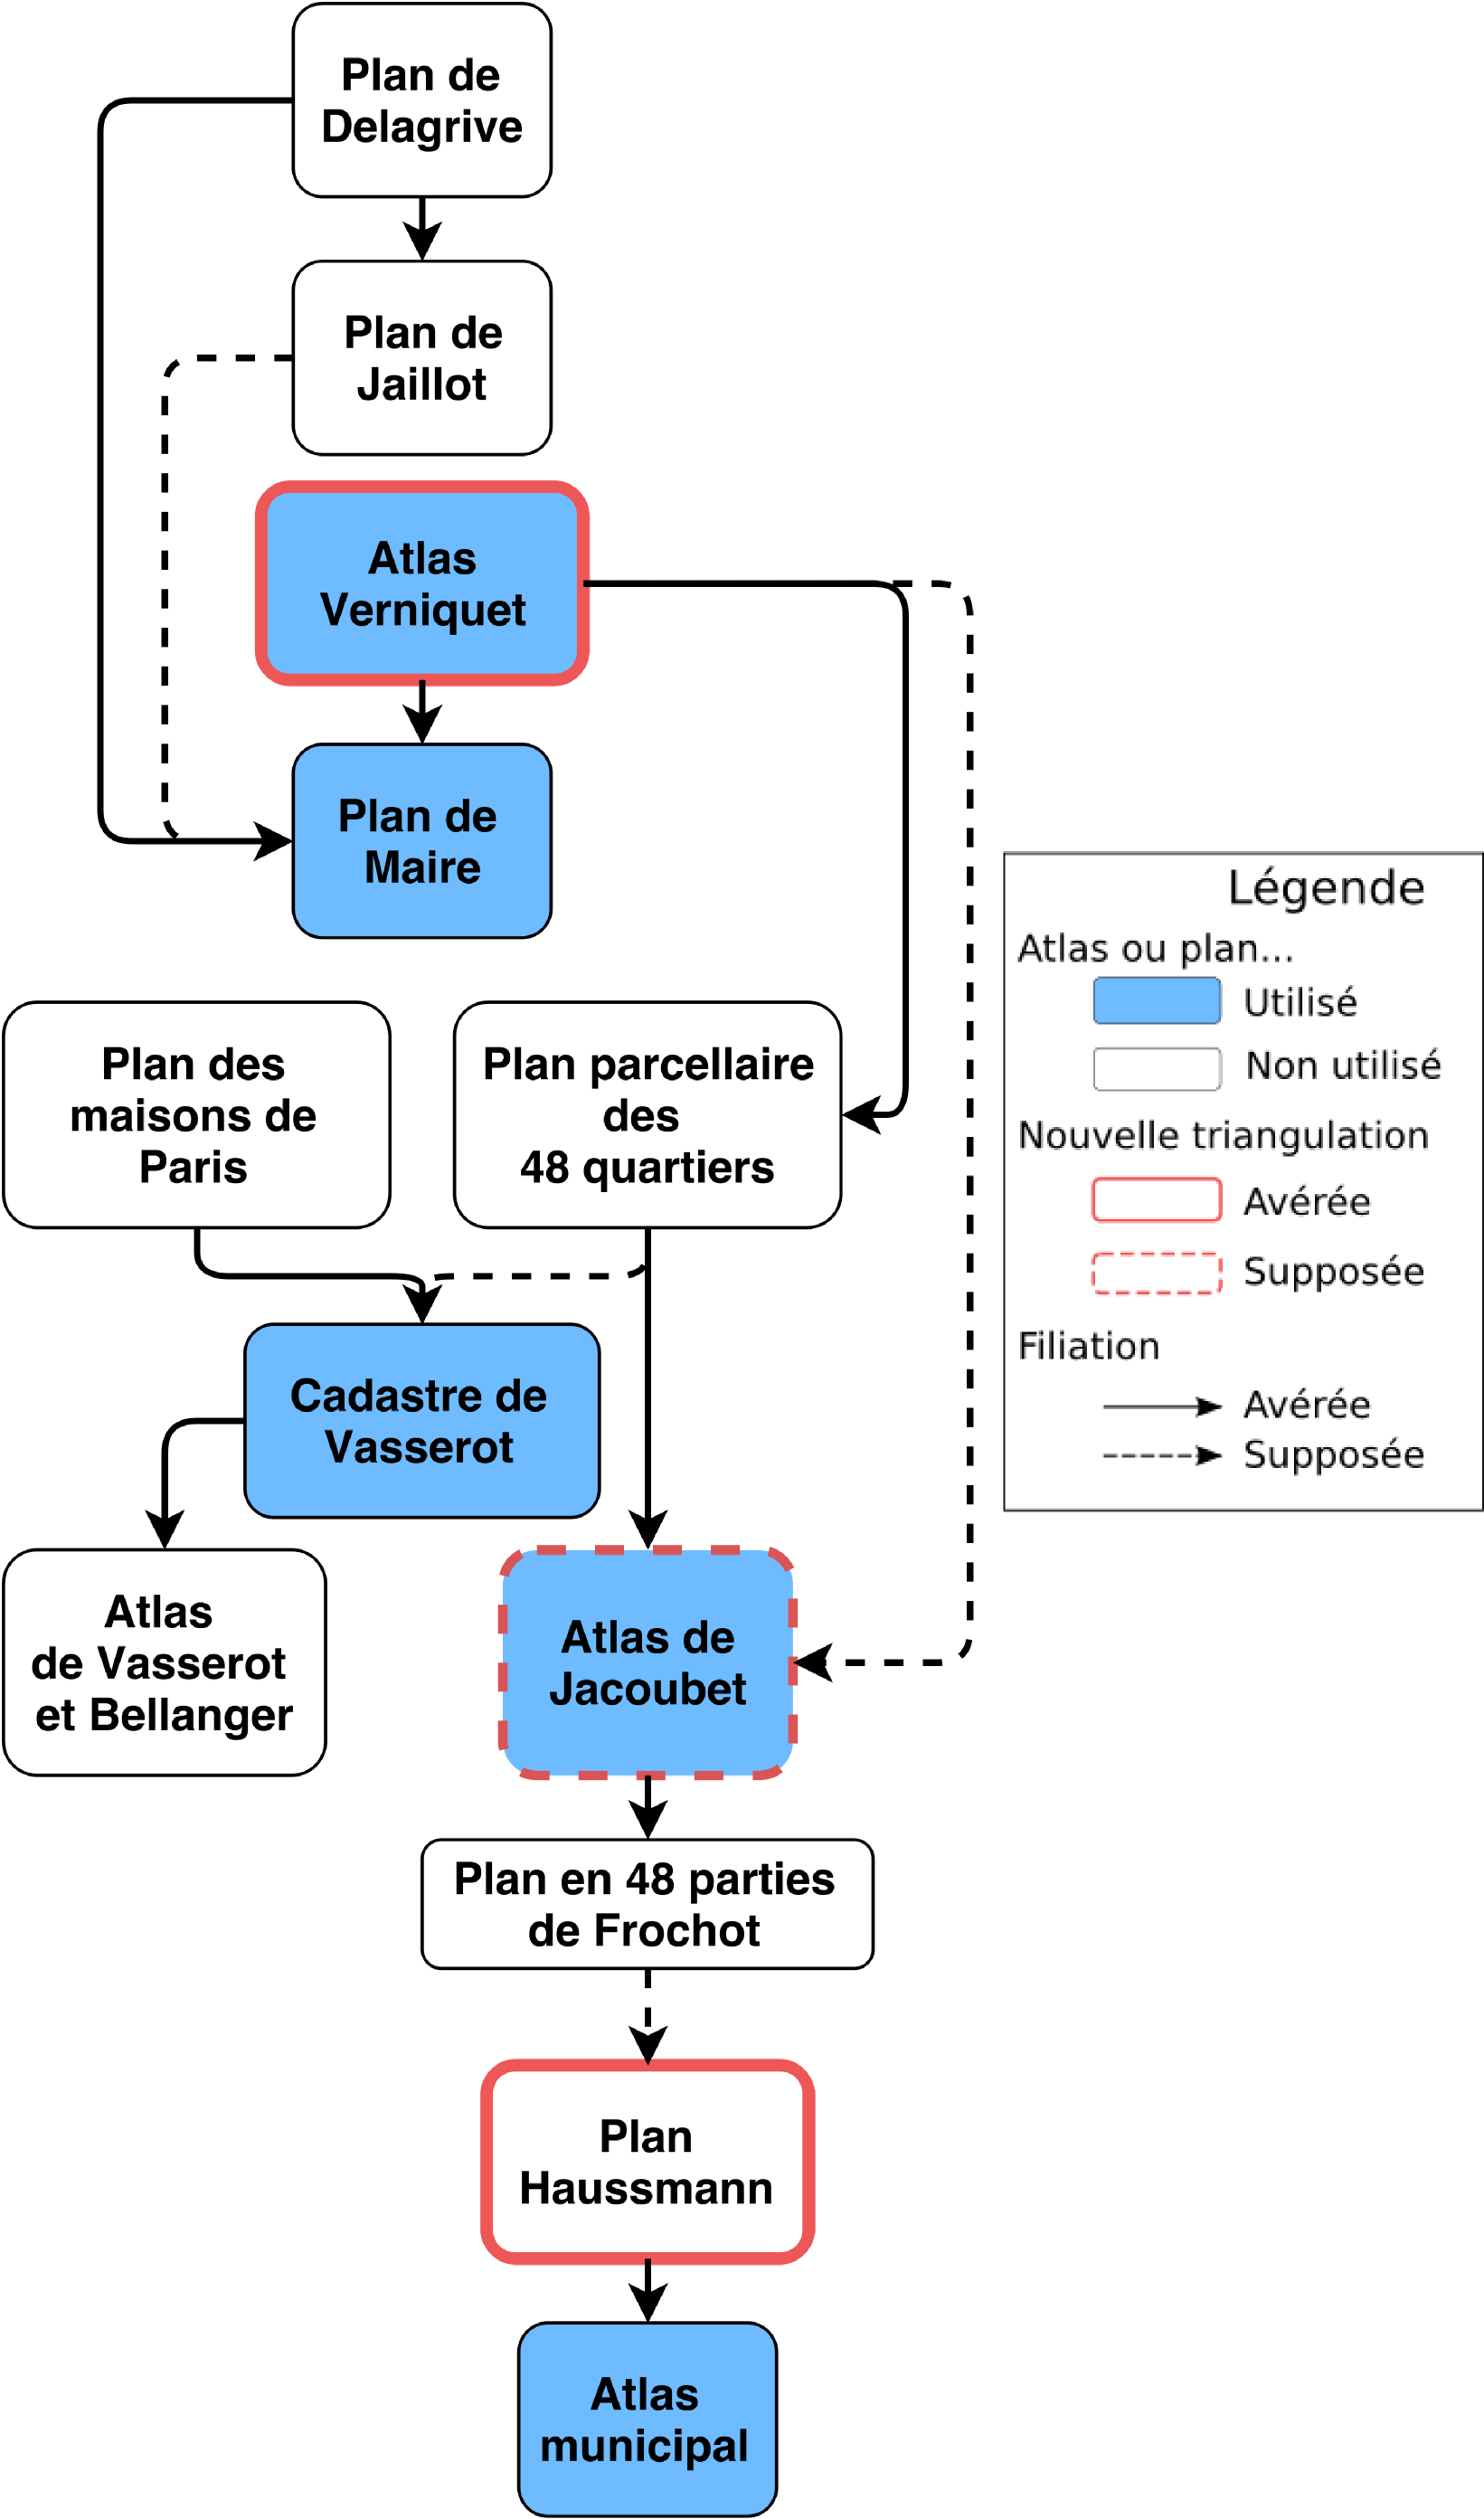
\includegraphics[width=0.7\textwidth]{filiations_entre_plans.png} 
	\caption{Filiations identifi�es entre les plans de Paris utilis�s dans la th�se.
Certains plans non utilis�s mais cit�s dans le chapitre sont �galement inclus car ils font partie de cette g�n�alogie}
	\label{fig:filiations}
\end{figure}


% 
% \subsection{Objets g�ohistoriques consid�r�s}
% %1p max
% \myparagraph{Rues}
% Rue de Sourdis = batiments de l'hotel de sourdis entierement reconstruits en 1840. Pas d'alignemen
% 
% \myparagraph{Les parcelles}
% C'est le lieu des propri�taires
% \clearpage
% 
% \subsection{Lieux d'�tude?}
% %1p max
% \myparagraph{Ile de la Cit�}
% Particularit�s du tissu urbain de Saint Martin des champs
% s
% \myparagraph{Saint Martin des Champs}
% Particularit�s du tissu urbain de Saint martin des champs
% \clearpage
% 
% 
% 
% \subsection{La transformation de la gestion de la ville par le prisme des plans}*
% Jean-Philippe Dumas, dans \citep{Dumas1999}
% free  lien Repr�sentation et description des propri�t�s � Paris au XIXe si�cle. Cadastre et plan parcellaire 
% 
% 
% \subsection{Conclusion}
% %1p max
% 
% \myparagraph{Le plan de Verniquet comme r�f�rentiel ancien}
% 
% \myparagraph{Ouvrir vers le mod�le}



% %@book{bonnardot1851,
%   title={�tudes arch�ologiques sur les anciens plans de Paris des XVIe, XVIIe et XVIIIe si�cles},
%   author={Bonnardot, A.},
%   lccn={07002479},
%  url={http://books.google.fr/books?id=\_G6kQHL0vNwC},
%   year={1851},
%   publisher={Deflorenne}
% }
% 
% %@article{Dumas1999,
% title =  {Repr�sentation et description des propri�t�s � Paris au XIXe si�cle. Cadastre et plan parcellaire},
%   author={Dumas},
% year = {1999}
% }
 % Dans ce chapitre on fait un peut d'histoire pour d�finir un peut mieux les objets que l'on manipule.
%\chapter*{Conclusion de la partie 1}

%---------------------PARTIE 2---------------------
\part[Construction de graphes spatio-temporels]{Construction de graphes spatio-temporels � partir de sources cartographiques anciennes}

\chapter{G�or�f�rencement des plans de Paris}
\renewcommand{\labelitemi}{\tiny$\blacksquare$}
\large \begin{mybox} \normalsize
\textbf{Objectifs~:} 
\vspace{11pt}
\begin{itemize}
\item  Proposer une approche permettant de g�or�f�rencer les atlas parisiens de fa�on pr�cise.
\vspace{11pt}
\item  Proposer une approche visant � analyser la qualit� g�om�trique des th�mes d'un plan topographique.
\vspace{11pt}
\item  Produire un corpus de donn�es g�ographiques vectorielles � partir des atlas g�or�f�renc�s.
\end{itemize}
\end{mybox}
\renewcommand\labelitemi{\textbullet}% bullet
\newpage
\minitoc
\newpage


Au travers du premier chapitre, nous avons vu que la recomposition des �tats d'un objet g�ohistorique pouvait �tre effectu�e en deux temps~: d'abord en extrayant de sources anciennes des repr�sentations de cet objet (le trac� d'une rue, le plan d'un b�timent, etc.), puis en les liant pour reconstituer l'objet g�ohistorique sous-jacent. Ces liaisons reposent sur l'identification de persistances et de changements entre repr�sentations cons�cutives. Les sources �tant cartographiques, la composante spatiale est un �l�ment fondamental de cette identification. Pour avoir une connaissance des propri�t�s spatiales des observations, deux �tapes sont n�cessaires~: une premi�re pour d�terminer leurs positions les unes par rapport aux autres ou par rapport � un r�f�rentiel spatial et une seconde pour extraire leurs formes des sources cartographiques.
\\
Le r�f�rencement des cartes pourrait �tre fait de fa�on relative en les mettant en correspondance avec une carte de r�f�rence � l'aide de m�thodes d'appariement d'images. L'application de telles m�thodes a par ailleurs �t� propos�e dans le contexte de cartes historiques par~\cite{Balletti2000}. Cependant, l'extraction d'observations g�ohistoriques permet d'envisager l'int�gration de bases de donn�es g�ographiques ext�rieures, anciennes ou r�centes pour enrichir la base de donn�es spatio-temporelle. Une seconde possibilit� consiste � situer les diff�rentes sources dans un r�f�rentiel commun, ind�pendant d'une source particuli�re.
Celles-ci d�crivant une portion de l'espace g�ographique, il est assez naturel de consid�rer ce dernier comme r�f�rentiel~: il s'agit donc de g�or�f�rencement. Les observations extraites de ces cartes g�or�f�renc�es sont localis�es dans un r�f�rentiel g�ographique commun d�s leur cr�ation, facilitant ainsi l'int�gration de donn�es g�ographiques externes.
\\
Dans ce chapitre, nous nous int�ressons dans un premier temps au g�or�f�rencement de nos sources cartographiques anciennes, puis � la vectorisation de leur contenu. Pour ce faire, nous proposons une approche de g�or�f�rencement adapt�e pour le cas sp�cifique des plans topographiques anciens de Paris. Afin d'introduire les particularit�s de cette approche, nous pr�sentons tout d'abord en section~\ref{section:section1} les probl�matiques pos�es par le g�or�f�rencement de plans dress�s avec des techniques et des connaissances g�od�siques particuli�res sur des r�f�rentiels r�cents. En section~\ref{section:georef_global}, nous pr�sentons en d�tail le processus de g�or�f�rencement ainsi que les notions li�es � la qualit� d'un g�or�f�rencement~\ref{section:qualitygeoref}, puis, en section~\ref{section:proposition} nous introduisons les adaptations que nous proposons pour le cas des plans de Paris. Cette proposition est par la suite test�e et valid�e en l'appliquant � l'atlas de Verniquet (\ref{section:verniquet}). Par la suite, nous montrons comment cette approche nous permet d'effectuer une analyse quantitative de la qualit� g�om�trique d'un plan. Ceci nous permet notamment de poser l'atlas de Verniquet comme un r�f�rentiel g�ographique g�om�triquement pr�cis sur l'espace ancien de Paris. Apr�s avoir appliqu� cette approche aux autres plans de Paris, nous pr�sentons en section (\ref{section:vectorisation}) le processus de vectorisation nous ayant permis d'extraire un ensemble de donn�es g�ographiques vectorielles pour chaque plan de Paris qui nous permettent de peupler notre mod�le de suivi d'objets g�ohistoriques.
\vspace{11pt}
\begin{figure}[ht!]
\centering
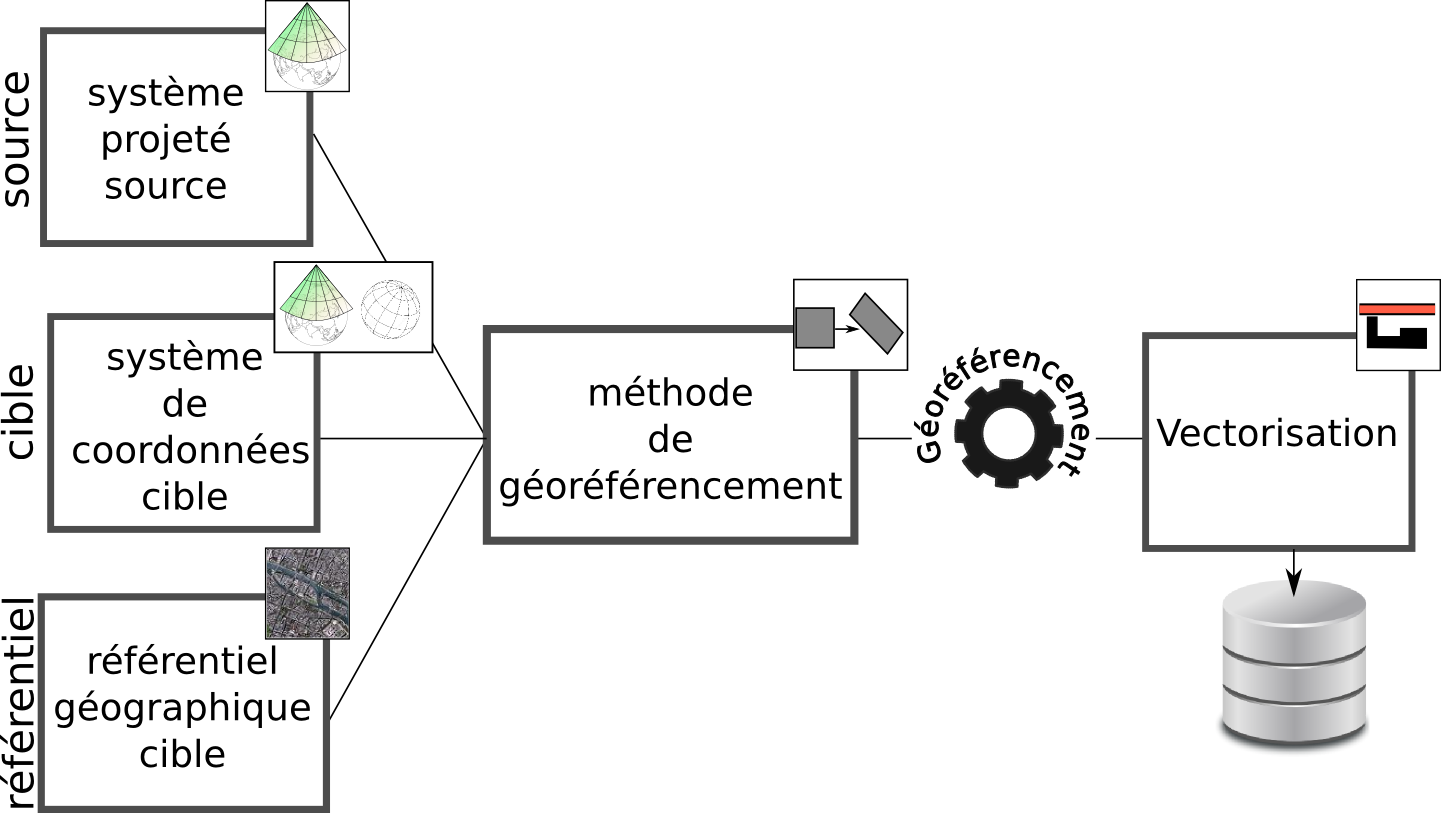
\includegraphics[width=0.8\textwidth]{schema_steps_intro.png}
                \caption{Sch�ma du chapitre 3.}
                \label{fig:shcme_chapter_3} 
\end{figure}

\section[Construire une carte topographique au XIX\up{e} si�cle]{De la Terre � la carte~: syst�mes de coordonn�es actuels et contemporains des atlas parisiens}
\label{section:section1}
%Le g�or�f�rencement indirect s'appuie donc sur l'identification, dans l'image � recaler, d'objets que l'on est capable de localiser � la surface de la Terre. Cette identification se d�roulant g�n�ralement visuellement, il est n�cessaire de disposer, d'une part, d'un mod�le de cette surface et, d'autre part, d'une repr�sentation, dans ce m�me mod�le, des objets rep�r�s comme points d'amer. Ainsi se d�finit le r�f�rentiel g�ographique d'un g�or�f�rencement.
%Intro brouillon

G�or�f�rencer un plan, c'est attribuer � une repr�sentation plate de l'espace des coordonn�es dans un mod�le de la surface terrestre. Diff�rents mod�les se sont succ�d�s au cours du temps dans le but d'approximer le mieux possible la forme complexe de la plan�te. L'�volution rapide de l'astronomie � partir du XVII\textsuperscript{e} si�cle a donn� lieu aux premiers mod�les math�matiques de la Terre sous la forme d'une sph�re. Les travaux des Cassini et d'autres astronomes de l'Acad�mie Royale des Sciences pour d�terminer le m�ridien de Paris et surtout sa position sur le territoire fran�ais, nomm� M�ridienne de France, ont fix� -au moins pour la cartographie fran�aise- un ensemble de rep�res g�od�siques pour les topographes et cartographes. 
\\
Cependant, les mod�les de la Terre tout comme le trac� de la m�ridienne ont continu� � �voluer. Aujourd'hui, ni le mod�le sph�rique du XVIII\textsuperscript{e} ni le m�ridien de Paris ne sont plus utilis�s et les donn�es g�ographiques sont localis�es suivant des mod�les plus complexes. La carte ancienne n'est donc pas une image simple, mais elle est elle-m�me associ�e � un mod�le de la Terre qu'il faut prendre en compte. Celui-ci est toutefois inconnu ou difficile � d�terminer avec pr�cision, faute de connaissances sur la phase de lev� topographique du plan. G�n�ralement, le mod�le de la carte ancienne est simplement ignor� et la carte consid�r�e comme une simple image, ce qui peut entra�ner des distorsions et des erreurs lors du g�or�f�rencement. � l'inverse, conna�tre le support g�od�sique sur lequel s'appuie un plan permet d'�liminer les erreurs li�es aux �carts entre mod�les pour ne conserver que celles des seules op�rations de lev�.
\\
Dans cette section, nous pr�sentons la strat�gie adopt�e en ce sens pour les atlas de Paris. En particulier, nous montrons que certaines sp�cificit�s de la cartographie parisienne li�es � sa proximit� avec le trac� physique de la m�ridienne de France\footnote{Voir le paragraphe \ref{paragraph:meridienne}} nous permettent d'utiliser des syst�mes de coordonn�es actuels comme �quivalents de ceux utilis�s au moment du lev� des plans. De cette fa�on, nous minimisons les distorsions des plans au moment du g�or�f�rencement dues aux �carts entre syst�mes actuels et syst�mes anciens.
\\
Dans ce but, nous revenons d'abord sur la fa�on de mod�liser la Terre et de localiser des objets g�ographiques � sa surface, puis nous aborderons rapidement les pratiques de lev� topographiques des cartographes parisiens aux XVIII\textsuperscript{e} et XIX\textsuperscript{e} si�cles. Enfin, nous pr�senterons le choix d'un syst�me de coordonn�es projet�es adapt� � nos atlas de Paris.

\subsection{Localiser un point sur la surface terrestre}
\myparagraph{Figures de la Terre}
Pour situer un point � la surface de la Terre de fa�on univoque, il faut d'abord disposer d'un mod�le d�crivant sa forme, g�n�ralement appel� \textit{figure de la Terre}. Celle-ci est complexe et irr�guli�re, soumise � des dynamiques d'origine g�ologiques (s�ismes, tectonique des plaques, �rosion, etc.) qui s'accumulent pour la distordre encore plus. Au cours de l'Histoire plusieurs mod�les de complexit� croissante ont �t� propos�s. Depuis l'hypoth�se de rotondit� de la Terre v�rif�e par �ratosth�ne et jusqu'au XVII\up{e} si�cle la plan�te a �t� approxim�e par une sph�re ( voir la figure \ref{fig:spheroide}). La sph�re de Picard, cr��e en 1670, est sans aucun doute l'une des plus connue. Les travaux de Huygens en 1673, puis ceux de Newton et Cassini montrent les limites du mod�le sph�rique, trop approximatif pour permettre des calculs de distances et d'angles pr�cis. Les calculs des deux derniers scientifiques, pourtant contradictoires, prouvent que la forme g�om�trique qui approxime le mieux la Terre n'est pas une sph�re mais un ellipso�de de r�volution (\ref{fig:ellipsoide}), c'est � dire une sph�re aplatie aux p�les. � partir de ce moment, de nombreux mod�les ellipso�daux apparaissent, certains d'entre eux restant encore aujourd'hui utilis�s, en particulier pour la cartographie. De tels mod�les simplifi�s ne conviennent cependant pas pour des mesures de haute pr�cision n�cessaires dans des domaines tels que l'a�ronautique. Ces consid�rations ont men� au dernier mod�le existant~: le g�o�de (\ref{fig:geoide}). Celui-ci repr�sente la surface du potentiel de pesanteur terrestre co�ncidant le mieux possible avec le niveau moyen des oc�ans. Autrement dit, il s'agit d'une approximation de la Terre affect�e par la r�partition des masses de mati�re dans la cro�te terrestre. Comme nous l'avons dit, l'ellipso�de est pr�f�r� en cartographie en raison des difficult�s � projeter sur la surface plane de la carte les irr�gularit�s dues au g�o�de. Afin de minimiser les erreurs li�es � l'approximation ellipso�dale, ces mod�les sont souvent locaux et adapt�s � des zones du g�o�de. Ces ellipso�des locaux sont donc choisis de fa�on � minimiser l'�cart entre leur surface et celle du g�o�de sur une �tendue donn�e. Ainsi, pour la France, le mod�le ellipso�dal IAG-GRS80 est utilis� depuis 2000 en remplacement de l'ellipso�de Clarke 1880 sur lequel �taient construits les syst�mes de projection cartographiques fran�ais Lambert I � IV~\citep{Girres2012}.
\begin{figure}[ht]
  \centering
        \begin{subfigure}[b]{0.3\textwidth}
                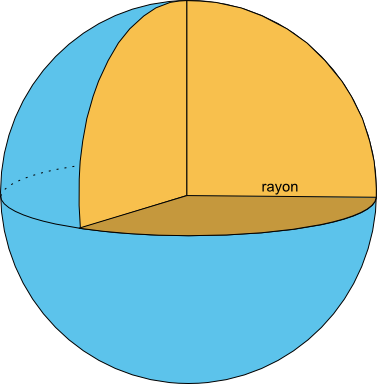
\includegraphics[width=\textwidth]{spheroide.png}
                \caption{Sph�ro�de}
                \label{fig:spheroide}
        \end{subfigure}%
~
	\begin{subfigure}[b]{0.3\textwidth}
                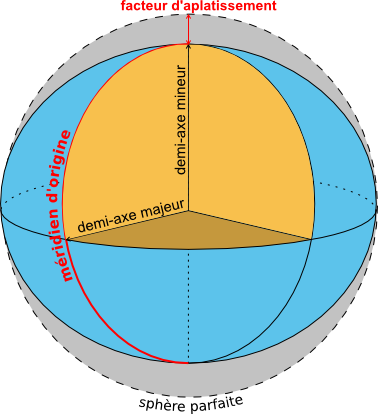
\includegraphics[width=\textwidth]{ellipsoide.png}
                \caption{Ellipso�de}
                \label{fig:ellipsoide}
        \end{subfigure}%
	\begin{subfigure}[b]{0.3\textwidth}
                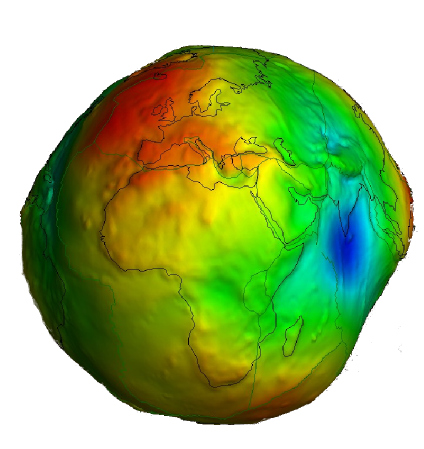
\includegraphics[width=\textwidth]{geoide.png}
                \caption{G�o�de}
                \label{fig:geoide}
        \end{subfigure}%
         \caption{Les trois figures de la Terre, ordonn�es par qualit� d'approximation croissante. L'aplatissement de l'ellipso�de est largement exag�r� dans cet exemple.}
	\label{fig:figuresdelaterre}
\end{figure}

\myparagraph{Syst�mes g�od�siques}
L'int�r�t d'une figure de la Terre est de pouvoir positionner des objets � sa surface.
 Un \emph{syst�me g�od�sique}, ou \emph{datum} est un ensemble de constantes et de m�thodes permettant de d�finir un rep�re affine qui assigne � chaque point de la Terre une coordonn�e unique \footnote{\url{http://education.ign.fr/sites/all/files/geodesie_systemes.pdf}}. Un syst�me g�od�sique se compose des �l�ments suivants~:
\begin{itemize}
\item un ellipso�de de r�f�rence d�fini par ses param�tres de demi-axes majeur et mineur, d'aplatissement et son �cart au centre des masses de la Terre,
\item un mod�le de g�o�de de r�f�rence permettant de mesurer des altitudes,
\item un syst�me de coordonn�es g�ographiques en trois dimensions associ� � un m�ridien d'origine sur l'ellipso�de de r�f�rence,
\item un r�seau de points g�od�siques qui sont des points de rep�re calcul�s avec une tr�s grande pr�cision dans le syst�me de r�f�rence.
\end{itemize}
Un datum g�od�sique est associ� � un \emph{r�seau g�od�sique}, un ensemble de points physiquement ancr�s dans le sol permettant de mesurer les variations des positions des points de la surface (en raison de la tectonique des plaques, des changements d'altitude, etc.) et de corriger les mesures. Certains datum sont \emph{locaux} car ils d�finissent en plus un ellipso�de de r�volution local destin� � amoindrir les approximations dues � l'ellipso�de de r�f�rence. Dans ce cas, on associe toujours � un ellipso�de local son positionnement par rapport au centre d'un syst�me standard\footnote{Actuellement, il s'agit du syst�me WGS84, utilis� notamment par le GPS.}. Les syst�mes comportent g�n�ralement au moins un syst�me de coordonn�es planes d�di� � la repr�sentation cartographique.
\\
Il existe un certain nombre de syst�mes g�od�siques standards, globaux ou locaux. En France, le syst�me global officiel depuis le 1\up{er} janvier 2001 est le \emph{r�seau g�od�sique fran�ais 1993} (RGF93), qui s'appuie lui-m�me sur le r�seau g�od�sique europ�en ETRS89\footnote{\emph{European Terrestrial Reference System 1989}}. Il remplace en particulier le syst�me local NTF \footnote{\emph{Nouvelle Triangulation de France}}, construit de 1884 � 1991 par raffinements successifs d'une triangulation sur le territoire de la France m�tropolitaine.
\\
Comme nous traitons de plans topographiques, nous ne nous attardons pas sur tous les constituants d'un datum, mais nous d�taillons seulement les syst�mes de coordonn�es planes.

%\myparagraph{Les syst�mes de coordonn�es g�ographiques}
%Les syst�mes de coordonn�es g�ographiques permettent de placer tout point de l'espace � la surface (et aux alentours avec l'altitude) d'un ellipso�de de r�volution qui d�finit deux rep�res de r�f�rence~: l'�quateur et le m�ridien de r�f�rence. Si l'ellipso�de est globale, Greenwich en constitue le m�ridien d'origine standard. Cependant, d'autres r�f�rences peuvent �tre utilis�es localement; ainsi la France utilise le m�ridien de Paris pour les syst�mes nationaux. Dans ce cas, on associe toujours � un ellipso�de local son positionnement par rapport au centre d'un syst�me standard\footnote{Actuellement, il s'agit du syst�me WGS84, utilis� notamment par le GPS.}, ce qui forme le \textit{datum g�od�sique}. 
%
%Les coordonn�es d'un point est alors l'�cartement angulaire par rapport � ces deux axes. L'angle entre le m�ridien et le point correspond alors � sa longitude $\lambda$ tandis que celui qui le s�pare de l'�quateur est sa latitude $\phi$. Enfin, on peut exprimer l'altitude du point par rapport � l'ellipso�de. 

\myparagraph{Projections cartographiques}
Nous l'avons dit, la cartographie impose de projeter dans un plan un espace pourtant irr�gulier et approximativement ellipso�dal. Or, il est impossible de d�velopper un ellipso�de en surface plane \citep{Pumain2010}. La solution est alors de projeter des parties de cet ellipso�de sur une surface qui est, elle, d�veloppable. La figure \ref{fig:proj} illustre comment un cylindre peut servir de surface de projection. Ce proc�d� a cependant des inconv�nients car il ne permet pas de conserver � la fois les angles et les surfaces, d�formant de fait les objets g�ographiques. De plus, ces alt�rations augmentent � mesure que la zone � projeter s'agrandit et que l'on s'�loigne du parall�le tangent � la surface de projection (correspondant aux lignes rouges sur la figure \ref{fig:proj}). Pour cette raison, il est n�cessaire de conna�tre parfaitement leurs effets, en particulier en ce qui concerne l'alt�ration lin�aire qui fausse le calcul des distances euclidiennes dans le syst�me projet�\footnote{L'alt�ration lin�aire se d�finit comme la variation des longueurs induite par le passage d'une figure de la Terre � une projection plane.}.

\begin{figure}[ht!]
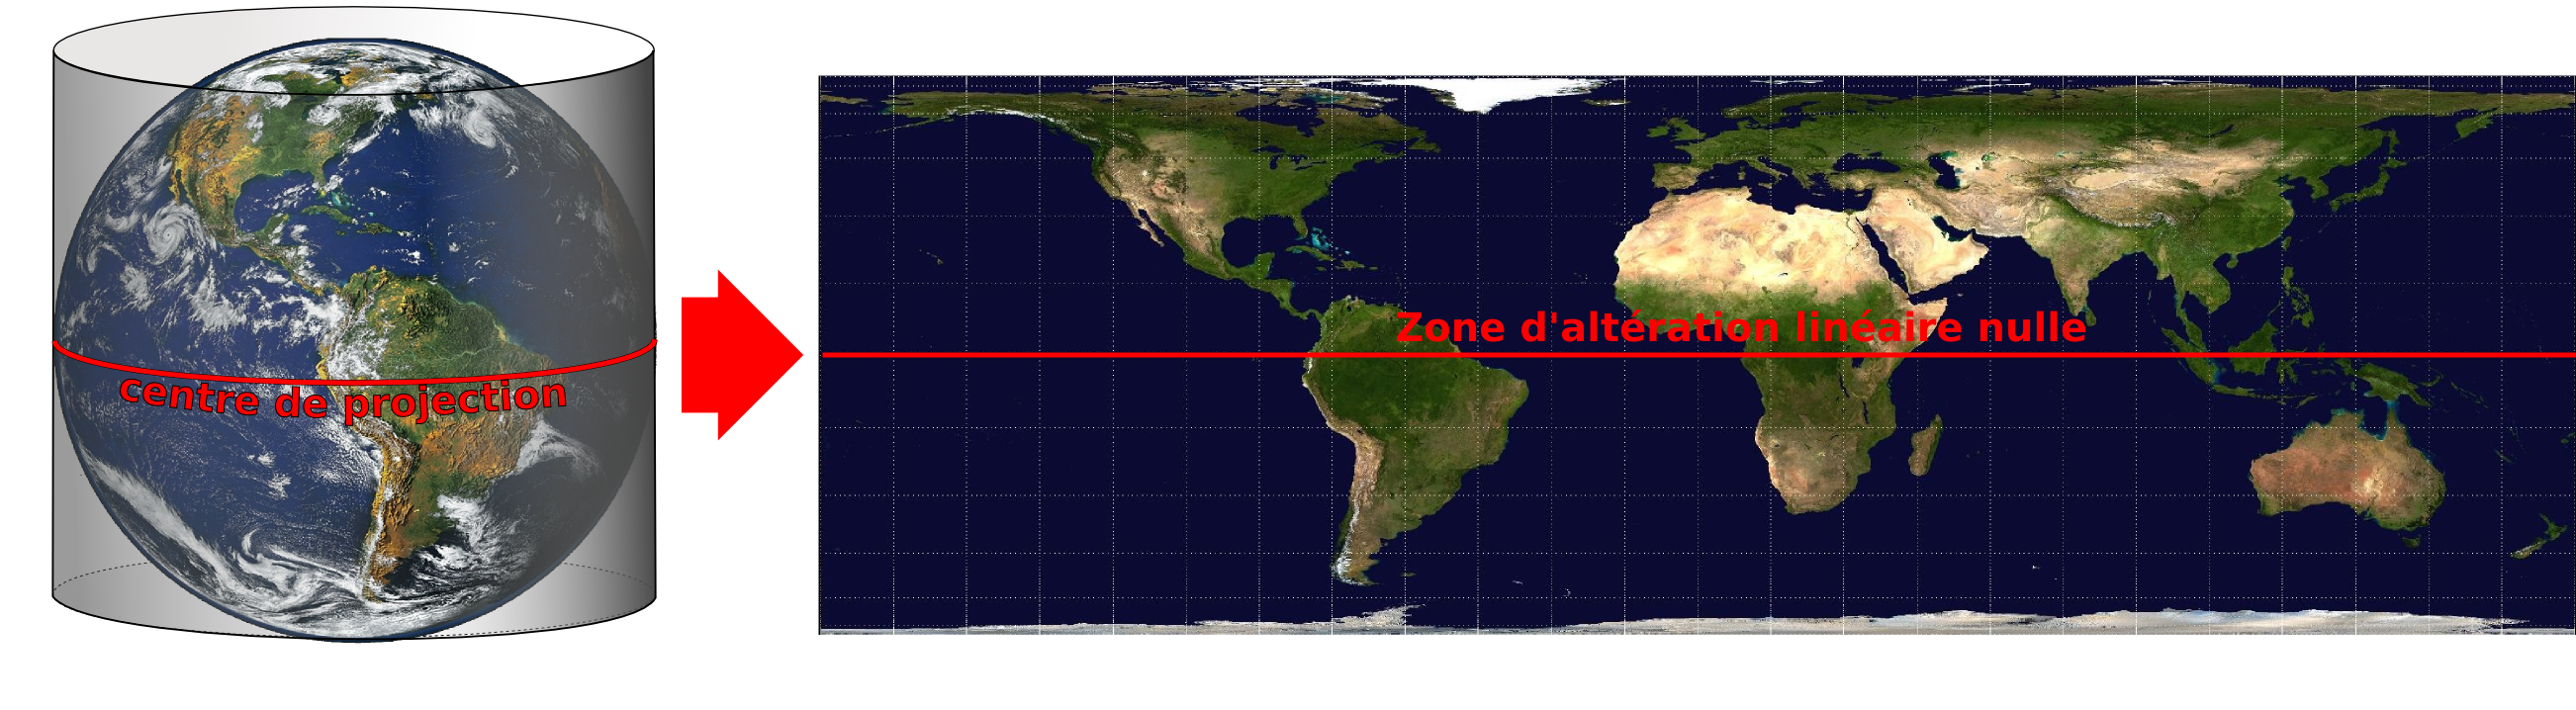
\includegraphics[width=\textwidth]{dev.png}
                \caption{D�veloppement de la surface terrestre sur un cylindre. Le parall�le tangent est situ� sur l'�quateur (projection Mercator).}
                \label{fig:proj} 
\end{figure}

Il existe trois types de projections cartographiques, dont deux sont d�finies selon qu'elles conservent~:
\begin{itemize}
 \item les angles seulement; on parle alors de projections conformes.
 \item les surfaces seulement; il s'agit de projections �quivalentes.
\end{itemize}
Une projection ne peut donc pas �tre conforme et �quivalente, mais elle peut ne conserver ni angles ni surfaces~: il s'agit alors de projection aphylactique.
\\
Au del� de ces trois types de projections, la surface d�veloppable choisie influe �galement sur le r�sultat. Trois d'entre elles sont particuli�rement usit�es, le cylindre, le c�ne et le plan (on parle alors respectivement de projections cylindriques, coniques et azimutales).
Il existe donc autant de cat�gories de projections qu'il est possible de combiner les surfaces d�veloppables et les types de projections. Par exemple, la projection Mercator, propos�e en 1569, conserve les angles et utilise un cylindre pour passer du globe � la carte, il s'agit donc d'une projection cylindrique conforme.

\myparagraph{De la Terre � la carte et son syst�me de coordonn�es}
Un syst�me g�od�sique muni d'une projection permet donc de passer de l'espace � la carte, c'est � dire attribuer � un objet situ� � la surface de la Terre des coordonn�es dans le plan. Ceci n�cessite finalement de conna�tre les param�tres suivants~:
\begin{itemize}
 \item un datum g�od�sique;
 \item un m�ridien d'origine qui permet de construire un rep�re de r�f�rence dans lequel exprimer les coordonn�es;
  \item un type de projection qui permet de conserver certaines caract�ristiques g�om�triques des objets.
\end{itemize}
Lorsque l'on souhaite replacer une carte ancienne dans un syst�me de coordonn�es g�ographiques, il faut effectuer une transformation de son syst�me de coordonn�es projet�es propre vers un syst�me de coordonn�es g�ographiques connu. Il faut donc connaitre les param�tres du syst�me de projection de la carte ancienne, ou tout du moins les approximer de fa�on � minimiser les erreurs lors de la transformation.
Lorsque l'�chelle des cartes est grande, comme � Paris, on peut supposer que ces alt�rations sont n�gligeables par rapport aux distorsions de la carte r�sultant d'erreurs de lev� et de l'alt�ration de la carte elle-m�me. 
\\
Nous allons maintenant explorer la fa�on de construire une carte aux �poques qui concernent nos plans de fa�on � estimer leur syst�me de projection.

\subsection{Cr�er une carte topographique aux XVIII\up{e} et XIX\up{e} si�cles}
\label{section:triangulation}
%Le choix d'un r�f�rentiel g�ographique adapt� � nos plans demande donc de choisir, dans un premier temps, un syst�me de projection dont on conna�t les particularit�s. Plus encore, puisque le g�or�f�rencement revient, dans notre cas, � effectuer un changement de syst�me, celui de la carte ancienne doit \emph{a priori} �tre aussi ma�tris�. 
En g�n�ral, le syst�me de projection d'une carte ancienne est peu connu parce que la carte finale ne comporte pas les indications g�od�siques de son relev� et que les minutes des relev�s topographiques se sont perdues. Ces informations sont d'autant moins connues que l'on recule dans le temps~: avant le XVII\textsuperscript{e} en France, aucun syst�me g�od�sique standard n'existe. Nos plans topographiques parisiens font 
cependant exception. En effet, ils apparaissent � une �poque de r�volution cartographique qui voit s'�tablir le premier syst�me g�od�sique pr�cis s'appuyant sur le m�ridien de Paris et la figure de la Terre sph�rique dite \emph{sph�re de Picard}. Afin de bien comprendre en quoi consiste la cr�ation d'une carte topographique � l'�chelle d'une ville aux �poques qui nous concernent, nous proposons de faire ici un point sur la m�thode g�om�trique adopt�e par les cartographes et g�om�tres pour transcrire le territoire sur une carte~: la triangulation. Nous verrons dans la section suivante que les particularit�s des plans topographiques de Paris permettent d'approximer leur syst�me de projection.

\myparagraph{La m�ridienne de France, socle des op�rations de triangulation � Paris}
\label{paragraph:meridienne}
Pour r�aliser un lev� topographique, il faut disposer d'un rep�re � partir duquel les coordonn�es des points relev�s seront exprim�es. Le calcul de la m�ridienne de France (aujourd'hui appel� ''m�ridien de Paris'') permet de fournir un rep�re absolu sur lequel tous les cartographes et ing�nieurs topographes peuvent s'appuyer, les coordonn�es �tant exprim�es par rapport � cette m�ridienne\footnote{Pour les latitudes, le rep�re est plus simple puisqu'il est fond� sur l'�quateur.}. Pour obtenir \emph{des cartes g�ographiques de la France plus exactes que celles qui ont �t� faites jusqu'ici}~\citep[p.235]{Martin2008}, l'astronome Jean Picard est nomm� par Colbert responsable de la r�alisation d'un ''Ch�ssis g�n�ral'' de la France~\citep[291--295]{Gallois1909}. Ce canevas g�od�sique repose sur deux �l�ments~:
\begin{itemize}
\item le relev� de la m�ridienne de Paris,
\item de la cr�ation d'un canevas de triangles couvrant toute la France s'appuyant sur cette m�ridienne;
\end{itemize}
La m�ridienne s'ancre alors physiquement dans Paris avec la construction de l'Observatoire Royal, termin�e en 1671, align� sur le trac� de la m�ridienne et travers�e par elle en son milieu. Le calcul de la m�ridienne de Paris allant de Dunkerque � Perpignan, issu du travail de Picard, puis de Jean-Dominique Cassini et Jacques Cassini, est termin�e en 1718 (voir la figure~\ref{subfig:MAPCassiniTriangles})\footnote{Cela signifie qu'un r�seau de points mat�rialis�s est g�or�f�renc�.}.
Afin de d�finir un plan dans lequel le canevas triangulaire de la France peut �tre r�alis�, cinq perpendiculaires � la m�ridienne sont ajout�es\footnote{Il ne s'agit pas de parall�les g�od�siques.}, dont une passant par l'Observatoire Royal, visible dans la figure \ref{subfig:MAPCassiniExtrait}
\\
Le canevas de triangles couvrant la France est quant � lui r�alis� par  C�sar-Fran�ois Cassini de Thury  � partir de 1756 pour la carte de m�me nom.
\begin{figure}[ht!]
\centering
        \begin{subfigure}[t]{0.51\textwidth}
                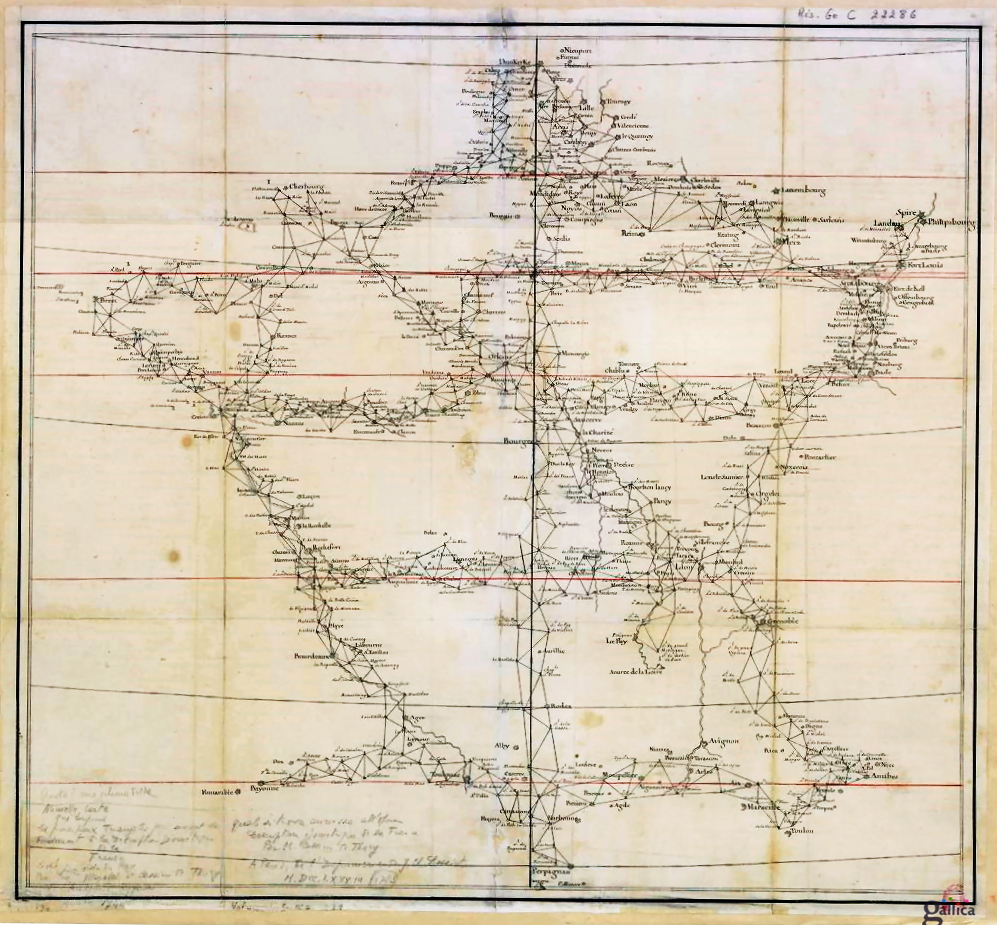
\includegraphics[width=\textwidth]{1744_canevas_cassini.jpg}
                \caption{Premier canevas et m�ridienne de France~\citep{MAPCassiniTriangles}}
	           \label{subfig:MAPCassiniTriangles}
        \end{subfigure}%
~
	\begin{subfigure}[t]{0.47\textwidth}
                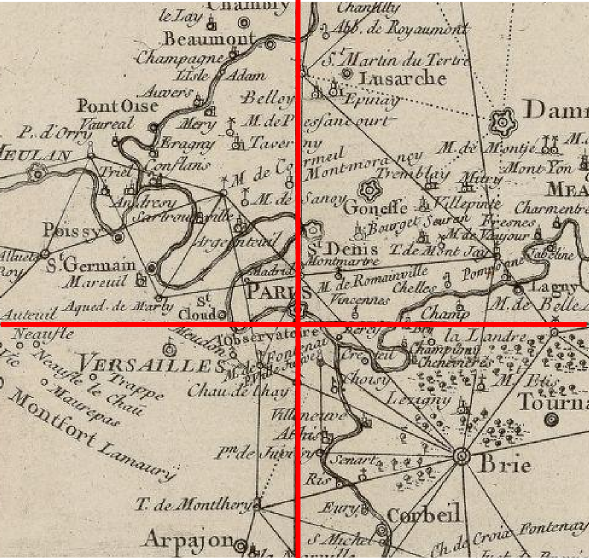
\includegraphics[width=\textwidth]{canevas_paris.png}
                \caption{D�tail � Paris. Extrait de~\citep{MAPCassiniExtrait}}
	           \label{subfig:MAPCassiniExtrait}
	\end{subfigure}%
\caption{Le premier canevas triangul� de la France, avec la m�ridienne et les cinq perpendiculaires (� gauche). La position de la m�ridienne et de sa perpendiculaire � Paris sont visible � droite~: on les voit se croiser � l'Observatoire.}
\end{figure}
%Objectif : expliquer que le calcul du m�ridien est quasi contemporain de Verniquet, et qu'il sera corrig� au cours du XIXe si�cle. Il change donc un peu en m�me temps que les plans.
%//WARN : todo + �a demande du travail d'�tat de l'art. En particulier sur les changements.
%\url{http://www.persee.fr/web/revues/home/prescript/article/geo_0003-4010_1909_num_18_100_6665?_Prescripts_Search_tabs1=standard&}
%\url{http://gallica.bnf.fr/ark:/12148/btv1b53083192q/f1.zoom} : la perpendiculaire
\myparagraph{Triangulations g�od�siques parisiennes}
L'id�e de la triangulation g�od�sique est de construire sur l'espace g�ographique un maillage triangulaire dont les longueurs et l'orientation sont connues par rapport � un rep�re (ici la m�ridienne)~\citep{Boutier2002}. Le maillage est r�alis� dans un espace plan de fa�on � n'utiliser qu'une trigonom�trie euclidienne. La m�ridienne est alors approxim�e localement par un segment de droite nomm� \emph{base}, ce qui oblige � cr�er plusieurs triangulations locales s'il faut couvrir une grande portion du territoire.
\\
La construction du maillage est un processus it�ratif, sch�matis� en figure~\ref{fig:schema_triangulation}. D'abord (point 1), une base AB de longueur et d'azimut connus est d�termin�e. Il s'agit g�n�ralement d'une portion de la m�ridienne. Un troisi�me point C correspondant � un rep�re visuel fixe (clocher, tour, colline, etc) est choisi et les angles $\alpha_1$ et $\alpha_2$ sont mesur�s (point 2). On peut alors construire le triangle ABC, puis recommencer avec un point D en utilisant un cot� du triangle ABC comme nouvelle base (point 3). 
\begin{figure}[ht]
  \centering
   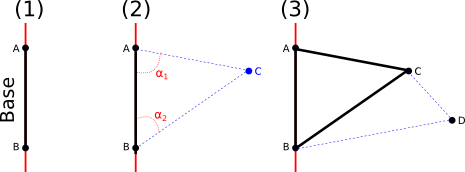
\includegraphics[width=0.8\textwidth]{triangulation.png}
         \caption{Sch�ma simplifi� des �tapes d'une op�ration de triangulation g�od�sique.}
   \label{fig:schema_triangulation}         
\end{figure}
� Paris, la proximit� de rep�res physiques de la m�ridienne (l'Observatoire Royal et deux mires plac�es aux extr�mit�s nord et sud de Paris) offre aux cartographes la possibilit� de cr�er des canevas de triangulation extr�mement complets. Souvent, ils s'appuient non seulement sur la m�ridienne mais �galement sur sa perpendiculaire passant � l'Observatoire Royal. La pr�cision g�om�trique devenant une pr�occupation majeure des cartographes de la fin du  XVIII\textsuperscript{e} si�cle, le canevas de triangulation est mis en avant et accompagne parfois m�me les atlas (c'est le cas pour les atlas de Verniquet et Jacoubet par exemple). %La figure \ref{figure:trianglesverniquet} montre ainsi le plan des triangles principaux lev�s par Edm� Verniquet pour la r�alisation de son atlas.
Dans le cas de la cartographique parisienne, qui impose un niveau de granularit� fin en descendant au niveau de la rue ou du b�timent, d'autres types de relev�s topographiques compl�tent la triangulation. En particulier, le lev� des rues est effectu� en tra�ant non plus des triangles mais des s�ries de segments formant des lignes bris�es dont l'orientation de proche en proche est connue et rapport�e � un triangle du canevas\footnote{En topographie, il s'agit d'un \emph{cheminement polygonal}. Les coordonn�es de chaque point du chemin peuvent �tre calcul�s si on conna�t les longueurs des segments et les angles de chaque paire de segments cons�cutifs.}. La figure~\ref{figure:cheminsverniquet} en pr�sente un exemple tir� des minutes de l'atlas de Verniquet.
\\
Tous nos atlas sont construits de cette fa�on, soit � partir d'une nouvelle triangulation, soit en r�utilisant des canevas existants\footnote{Tout comme les cartes France enti�re de Cassini ou d'�tat Major}. Tous les relev�s topographiques de nos atlas sont donc effectu�s dans un syst�me de coordonn�e projet� relatif � la m�ridienne de France.
  \begin{figure}[ht!]
\centering
                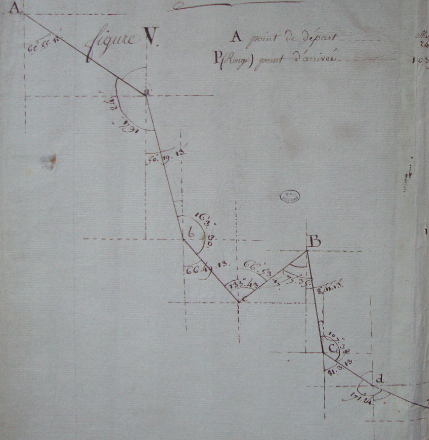
\includegraphics[width=0.5\textwidth]{lignepolyverniquet.png}
                \caption{Cheminement polygonal pour le relev� d'une rue. Extrait des minutes de l'atlas de Verniquet.}
	           \label{figure:cheminsverniquet}
\end{figure}
 
%Peut etre un point sur le fait que les sommets des triangles sont pour la plupart plac�s sur des lieux qui ont disparu?
%//WARN : todo + �a demande du travail d'�tat de l'art.
%Sur l'extrait de Verniquet, la perpendiculaire est � 7.2 (ouest), 7.4, 7.2 (est) cm du mur exterieur, ce qui fait (a une echelle de 11.8cm pour 5 toises) environ 3m�tres (3.05-3.13)

%\myparagraph{Choix d'une projection cartographique}
%Le choix d'une projection dans laquelle transformer les plans parisiens doit �tre guid� par l'alt�ration lin�aire locale, qui doit �tre minime. Cependant, il est �galement important que le syst�me choisi soit, sinon standard, au moins commun pour faciliter l'int�gration de donn�es suppl�mentaires, r�centes notamment. Puisque nos plans sont tous construits sur des triangulations locales � Paris avec pour origine la m�ridienne de France mais que nous ne les connaissons pas avec pr�cision, il est pertinent de choisir une projection qui les approximent suffisamment bien localement. Pour cette raison, nous avons privil�gi� le syst�me Lambert I qui pr�sente l'avantage de s'appuyer sur le m�me lieu d'origine et dont l'alt�ration aux alentours est, sinon nulle, consid�r�e n�gligeable car de l'ordre de quelques millim�tres par kilom�tre. De plus, la plupart des SIG permettent aujourd'hui de transformer une carte projet�e en Lambert NTF vers le Lambert 93, ce qui permet de replacer au besoin les plans dans un syst�me officiel. Le passage entre les deux syst�mes n'est cependant pas trivial et n�cessite l'utilisation d'une grille de transformation, int�gr�e dans les principaux outils de projection cartographiques.

\section{G�or�f�rencement~: principe de la m�thode usuelle}
\label{section:georef_global}
G�or�f�rencer un plan topographique est une op�ration qui consiste � situer ce plan dans un rep�re g�ographique muni d'un syst�me de coordonn�es g�ographiques dans le but de croiser les informations qu'il contient avec celles d'autres repr�sentations de l'espace~\citep{Balletti2006}. En g�n�ral, le plan lui-m�me poss�de un syst�me de coordonn�es projet�es. La figure~\ref{figure:georef_global} illustre le processus de g�or�f�rencement de fa�on tr�s g�n�rale. Un g�or�f�rencement repose sur trois param�tres~:
\begin{enumerate}
\item le syst�me de coordonn�es projet�es de la carte source � g�or�f�rencer,
\item une m�thode de transformation,
\item un syst�me de coordonn�es cible (g�ographique ou projet�) dans lequel transformer la source.
\end{enumerate}
Conna�tre le syst�me de projection de la source est cependant optionnel. En effet, si on ne conna�t pas le syst�me source on utilise des points de rep�re pour projeter directement l'image dans le rep�re cible.
\\
Dans la section pr�c�dente, nous avons d�termin� le premier de ces trois points. Dans cette section, nous allons d�tailler le processus de transformation lui-m�me.
\begin{figure}[ht!]
  \centering
        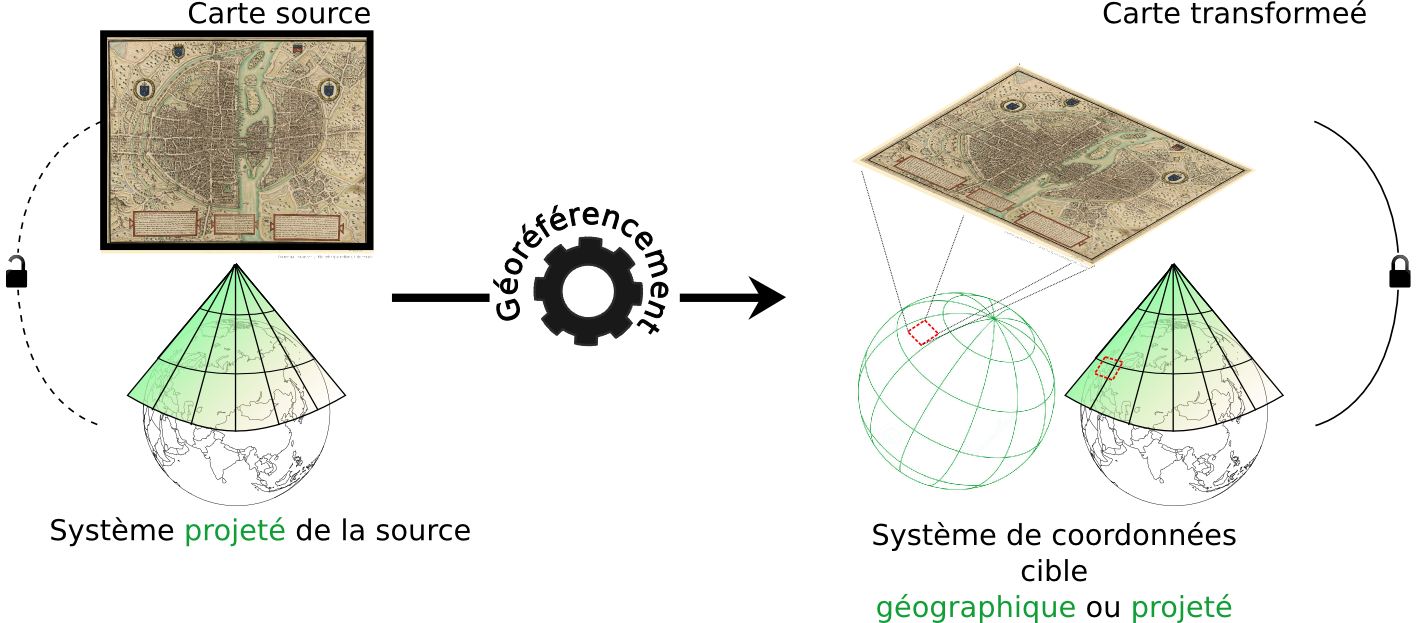
\includegraphics[width=0.8\textwidth]{georef_schemas.png}
         \caption{Sch�ma global du g�or�f�rencement}
	\label{figure:georef_global}
\end{figure}

\subsection{Types de g�or�f�rencements}
\myparagraph{Une m�thode particuli�re de recalage d'images}
Le g�or�f�rencement de cartes appartient au domaine de la g�od�sie et est li� aux m�thodes de recalage d'images (ou mise en correspondance d'images), qui consistent � optimiser un crit�re de similarit� entre deux images~\citep[pp.11--12]{Zhang1993}. Recaler des images entre elles est un probl�me g�n�ral qui sert, selon les disciplines, des desseins vari�s~: fusion d'informations, d�tection de changements, reconstruction 3D � partir d'images st�r�oscopiques, reconnaissance de formes. Les m�thodes de recalage sont class�es en trois cat�gories, selon le crit�re utilis�~\citep{Brown1992}. Les m�thodes \textit{g�om�triques} utilisent des crit�res mesurant la correspondance entre des primitives g�om�triques communes aux deux images. Elles peuvent �tre intrins�ques � l'image (points, contours, etc.) ou d�pendantes des appareils d'acquisition (capteur, orientation de l'appareil, etc.). Une autre cat�gorie, fond�e sur l'intensit�, traite des images dans leur totalit� en supposant qu'elles sont li�es par une relation affine ou d'�galit�~: il s'agit des m�thodes \textit{iconiques}. Il existe enfin des m�thodes hybrides associant des processus issus � la fois des m�thodes g�om�triques et iconiques.
\\
Quelque soit la m�thode choisie, il est n�cessaire de d�finir une~\textbf{fonction de transformation} que l'on note $F : I_s \rightarrow I_c$ dont l'objectif est de maximiser la valeur d'un crit�re de similarit� entre une image source $I_s$ et une image cible $I_c$. Si cette fonction d�pend du type de donn�es � projeter, son objectif est constant~: appliqu�e � l'image source, elle la projette dans le rep�re de l'image cible. Dans le cas du g�or�f�rencement, les images sources et cibles ont la particularit� de poss�der des syst�mes de coordonn�es g�ographiques ou projet�s.
\\
Il existe deux approches du g�or�f�rencement, compl�mentaires, nomm�es respectivement \textit{directe} et \textit{indirecte} s'appuyant sur les propri�t�s de l'image ou sur des primitives g�om�triques contenues dans celle-ci.

\myparagraph{Le g�or�f�rencement direct}
\label{paragraph:direct_georef}
Le g�or�f�rencement direct est essentiellement utilis� en photogramm�trie pour situer des donn�es de t�l�d�tection\footnote{Images a�riennes ou satellitaires, relev�s RADAR, LiDAR ou laser, etc.} � la surface de la Terre. Il s'agit d'un recalage dans lequel la transformation spatiale est directement calcul�e � partir de l'orientation de l'image par rapport au r�f�rentiel g�ographique, d�termin�e gr�ce aux param�tres internes et externes du capteur. Les premiers d�pendent de la nature du capteur (position du point principal, focale, distorsions de la lentille), tandis que les seconds sont g�n�ralement calcul�s � l'aide d'une centrale inertielle et d'un GPS \citep{Schaer2003}. Nous n'entrerons pas plus avant dans les d�tails, le g�or�f�rencement direct n'�tant pas le propos de notre travail. Il est cependant important de comprendre  qu'une telle m�thode implique deux choses. D'une part, elle n'est utilisable qu'� condition de conna�tre parfaitement les propri�t�s des outils ayant permis l'acquisition de l'image. D'autre part, elle suppose une ma�trise maximale des distorsions de l'image pour qu'elles soient rectifi�es par la transformation.
%
%\myparagraph{G�or�f�rencement direct}
%Le g�or�f�rencement direct est essentiellement utilis� en photogramm�trie pour situer des donn�es de t�l�d�tection\footnote{Images -a�riennes ou satellitaires-, relev�s RADAR, LiDAR ou laser, etc.} � la surface de la Terre. Son principe g�n�ral est relativement simple~: a partir d'une position connue (par GPS ou centrale inertielle) et si l'on conna�t les param�tres de position et d'orientation interne du capteur utilis� pour l'acquisition, on peut calculer la fonction de transformation depuis le rep�re local du capteur vers l'espace g�ographique, et donc g�or�f�rencer directement les donn�es \citep{Schaer2003}. Cette m�thode, pour �tre exacte, n�cessite une connaissance parfaite des outils d'acquisition de l'image. Elle suppose �galement l'absence de d�formations de celle-ci, ou du moins la connaissance \emph{a priori} des d�formations qu'elle contient.


\myparagraph{G�or�f�rencement indirect}
Il s'agit cette fois du proc�d� utilis� dans le cas o� l'on ne conna�t pas \emph{a priori} les param�tres de la fonction de transformation $F$. Ceux-ci sont alors estim�s gr�ce � l'identification d'�l�ments communs � l'image et � l'espace g�ographique. Le plus souvent il s'agit de points, d�sign�s dans la litt�rature de diff�rentes fa�ons~: \textit{points de contr�le}, \textit{de calage}, \textit{d'amer} ou encore \textit{d'appui} selon les domaines. On pr�f�rera ici le terme de \textbf{point d'amer}, qui d�signe un objet fixe et remarquable. Lorsque l'on dispose de deux images $I_1$ et $I_2$, on notera deux points d'amer correspondant � des �l�ments communs dans $I_1$ et $I_2$ par le couple $(p,p')$ o� $p$ est un point dans $I_1$ et $p'$ un point dans $I_2$. La figure~\ref{figure:amer} pr�sente un exemple de points d'amer plac�s sur l'H�tel des Invalides � Paris. Le crit�re de similarit� utilis� d�pend d'une repr�sentation de la Terre. La distance euclidienne entre les points d'amer est la plus souvent utilis�e quand cette repr�sentation est situ�e dans le plan. Dans les autres cas, des distances g�od�siques sont plus adapt�es\footnote{La distance g�od�sique est une distance � la surface d'un ellipso�de. Par commodit�, elle est souvent approxim�e par la distance euclidienne.}. Notons �galement que des primitives g�om�triques plus complexes que des points peuvent �tre utilis�es comme �l�ments communs. Par exemple,~\cite{Baiocchi2005} s'appuient sur des structures lin�aires pour g�or�f�rencer une carte ancienne de Rome. De la m�me fa�on, \cite{Papakosta2012} utilisent le trac� de routes et de cours d'eau pour g�or�f�rencer d'anciennes vues a�riennes de Gr�ce.
\begin{figure}[ht!]
  \centering
        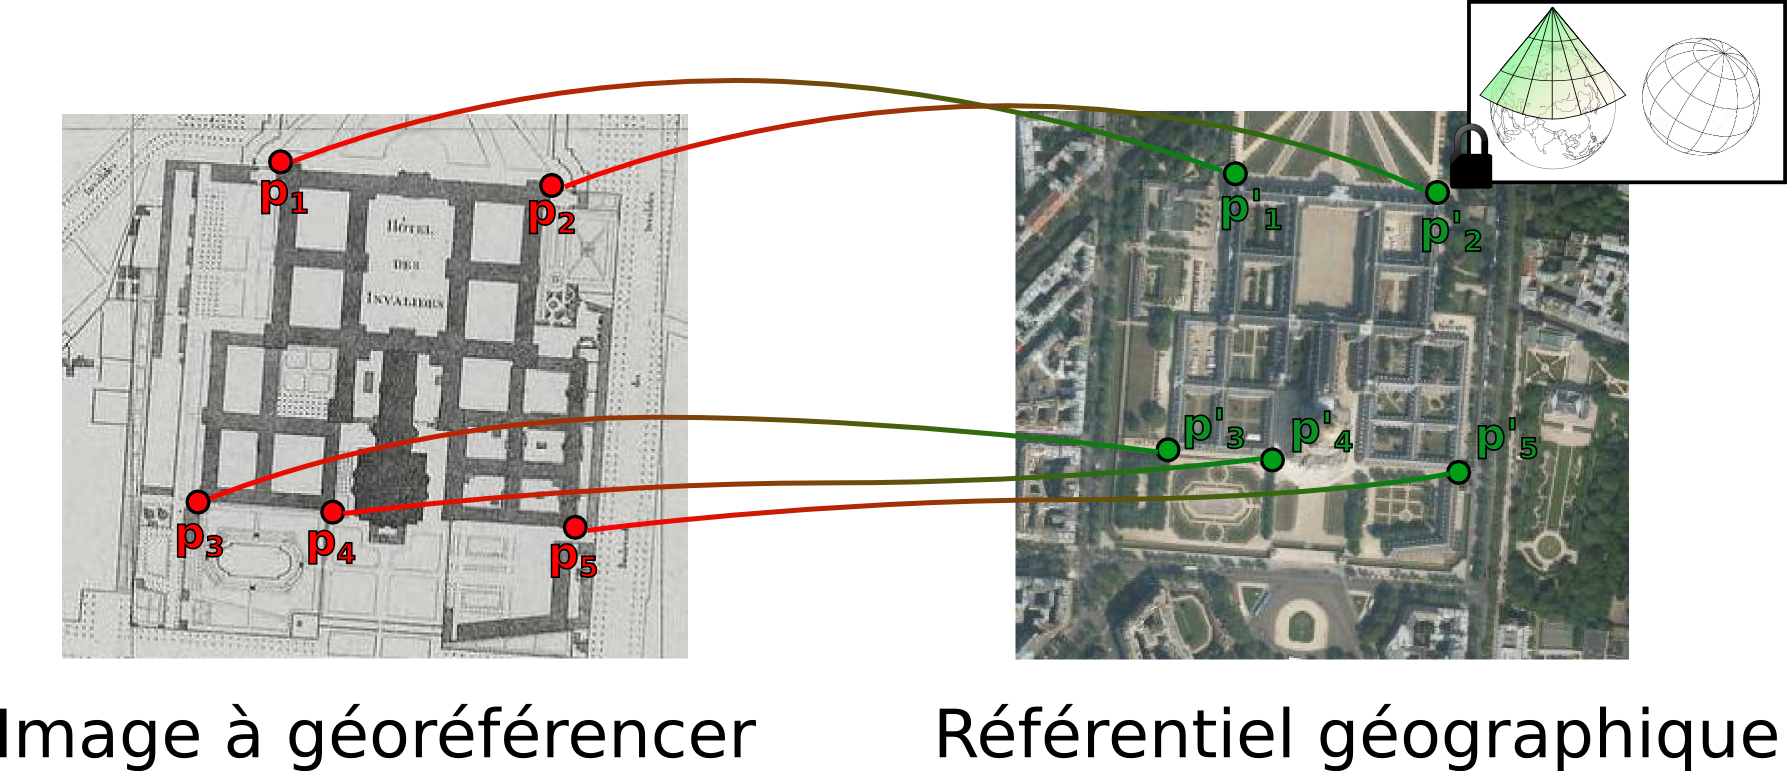
\includegraphics[width=\textwidth]{detail_amer.png}
         \caption{Un exemple de placement de points d'amer}
	\label{figure:amer}
\end{figure}


\myparagraph{Le cas des cartes anciennes}
Dans le cas o� les images recal�es sont des cartes anciennes, la m�thode directe appara�t inapplicable. D'une part, le syst�me de coordonn�es projet�es de la source -la carte ancienne- est g�n�ralement inconnu (voir la section~\ref{section:triangulation}). D'autre part, les cartes, proposant des repr�sentations visuelles vari�es, sont peu adapt�es � un g�or�f�rencement direct s'appuyant sur des similarit�s entre propri�t�s des images. C'est pourquoi dans la suite de cette th�se, nous avons recours � la m�thode indirecte fond�e sur l'identification de points d'amer. Cependant, nous devons �tre conscient d'une limite importante de la m�thode indirecte, en particulier pour des cartes anciennes. Le placement de points d'amer sur un r�f�rentiel r�cent est parfois difficile en raison de la trop forte �volution du territoire qui emp�che l'identification de points homologues. Or dans l'espace urbain en forte mutation qu'est Paris au tournant du XIX\up{e} si�cle, rien n'est plus incertain que la d�couverte de tels points, en particulier dans les zones p�riph�riques. En r�alit�, la plupart les faubourgs de l'Ancien R�gime disparaissent enti�rement sous les nouveaux lotissements des ann�es 1820-1830; la figure \ref{fig:changes_roule} le montre sur l'ancien espace du faubourg du Roule. On y voit tr�s clairement la rupture provoqu�e par l'op�ration immobili�re entre les plans de 1808 et 1836 qui �pargne presque uniquement la rue du Rocher (elle m�me pourtant �largie et align�e). Visuellement, l'espace de 1775 � 1808 n'a plus rien de commun avec celui de 1836-2010. 
\begin{figure}[ht]
 \centering
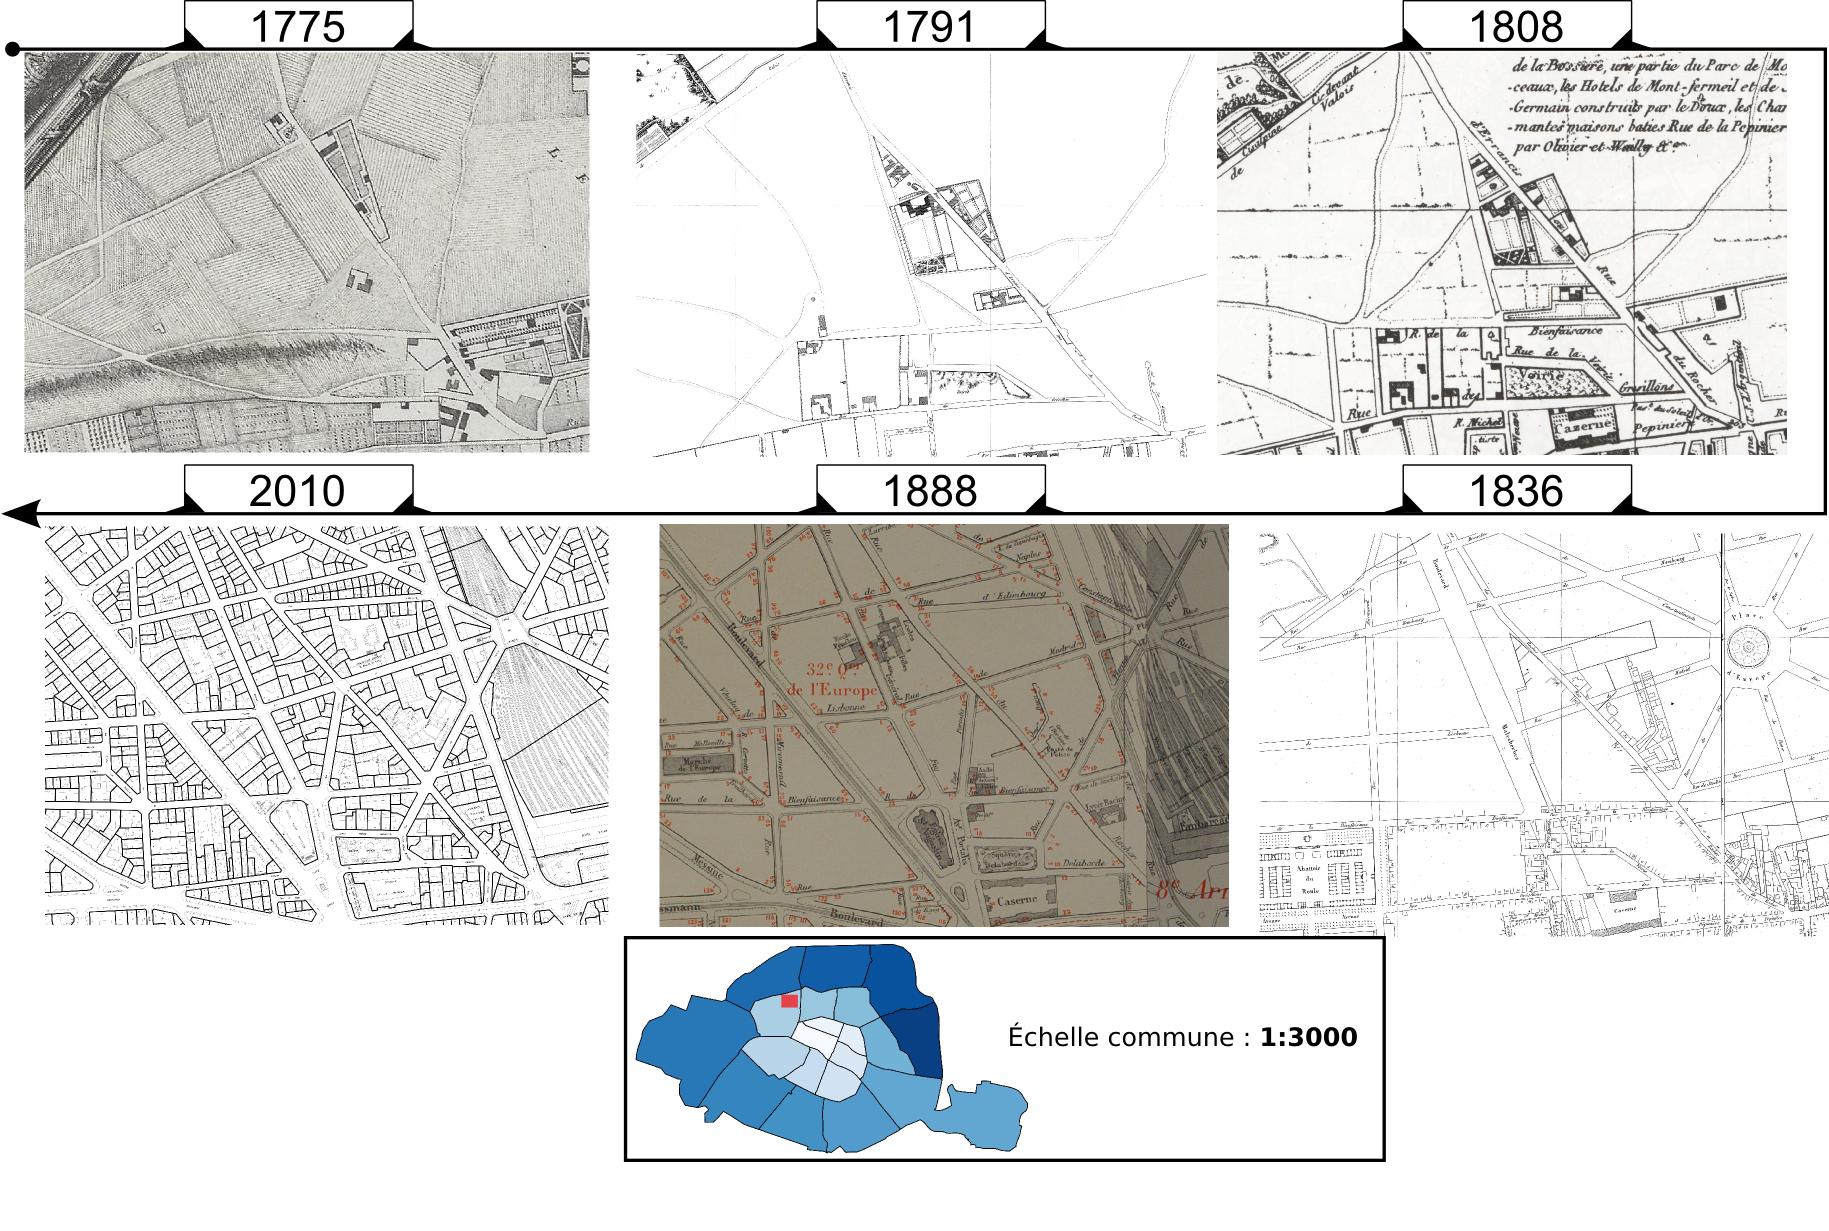
\includegraphics[width=0.90\textwidth]{changes.png} 
	\caption{Transformations entre 1775 et 2010 du faubourg parisien du Roule. Le bouleversement total de la zone se per�oit dans l'�cart entre les plans de 1808 et 1836. L'espace de 2010 n'a plus rien de commun avec celui du XVIII\up{e} si�cle~: presque aucun �l�ment commun n'est rep�rable.}
	\label{fig:changes_roule}
\end{figure}

\subsection{Principe d�taill� du g�or�f�rencement indirect}
Il appara�t donc que le g�or�f�rencement indirect est la m�thode la plus adapt�e pour recaler les plans topographiques de Paris. Nous la pr�sentons en d�tail dans cette section. De cette fa�on, nous d�gageons les contraintes pos�es par ce processus, en particulier lorsqu'il concerne des cartes anciennes.

%Nous avons montr� en quoi le syst�me de projection cartographique de la carte ancienne jouait un r�le majeur lorsqu'il s'agit de recaler des cartes topographiques anciennes. Afin de comprendre comment ces diff�rents �l�ments s'associent lors d'un g�or�f�rencement il faut en expliquer le processus. Cette section s'attachera donc � d�crire les �tapes constitutives d'un g�or�f�rencement indirect appliqu� en particulier aux cartes anciennes.

\myparagraph{�tapes du processus}
Le principe que nous pr�sentons ici n'est pas sp�cifique aux cartes anciennes. Il s'agit du processus de g�or�f�rencement indirect tel qu'il est r�alis� par la majorit� des SIG. Deux cas g�n�raux peuvent se pr�senter~: soit le syst�me de projection de l'image source est connu, soit il ne l'est pas. Le sch�ma en figure~\ref{figure:georef_indirect_detail} pr�sente les �tapes majeures d'un tel processus dans les deux cas. Il se situe apr�s le placement de points d'amer dans l'image source (le plan ancien) et dans le rep�re g�ographique ou projet� cible. Le d�roulement est le suivant~:
\begin{enumerate}
\item on choisir des points d'amer sans ambigu�t�, qui existent toujours aujourd'hui et qui sont facilement pointables,
\item les points d'amer d�finis dans le rep�re de la carte source sont projet�s dans le syst�me de coordonn�es projet�es de cette image - point (1) sur le sch�ma\footnote{Projeter l'image dans son syst�me de coordonn�es revient � affecter � chaque pixel sa coordonn�e dans ce syst�me. Si la carte n'est pas d�form�e, il s'agit d'une simple transformation affine.}. Si celle-ci n'en poss�de pas (parce qu'il est inconnu, ou parce qu'il s'agit d'une simple image), cette �tape est ignor�e. On se trouve alors dans le second cas de figure, 
\item une transformation spatiale $F$ est estim�e � partir des point d'amer de l'image source et leurs correspondants dans le syst�me de coordonn�es cible. Cette �tape sera d�taill�e dans le prochain paragraphe,
\item l'image source est transform�e par $F$ vers le syst�me de coordonn�es cible. Elle est alors potentiellement �tir�e et d�form�e.
\end{enumerate}

\begin{figure}[ht!]
  \centering
        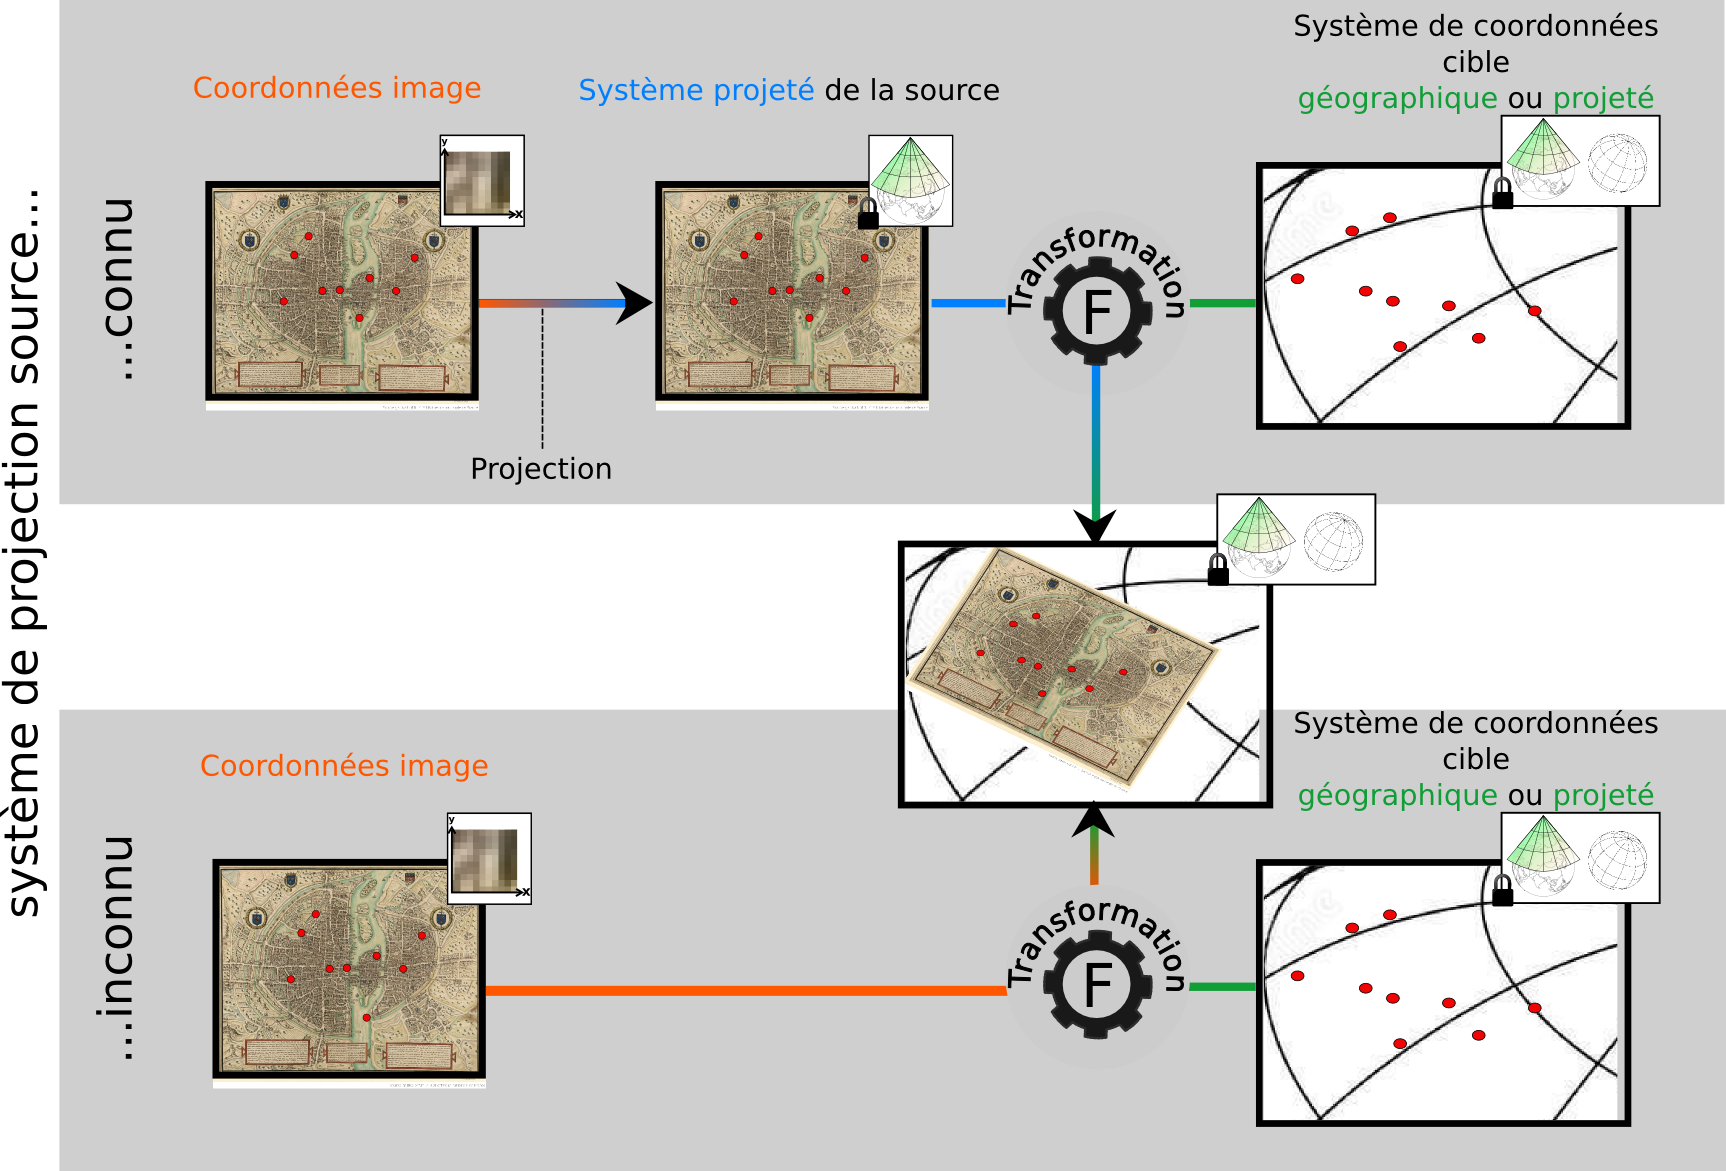
\includegraphics[width=\textwidth]{georef_schemas_detail.png}
         \caption{D�tail du processus de g�or�f�rencement indirect}
	\label{figure:georef_indirect_detail}
\end{figure}


\myparagraph{Forme de la transformation spatiale $F$~: cas de figures possibles}
La transformation de l'image source vers le r�f�rentiel cible n�cessite trois �tapes. D'abord, une premi�re projection est effectu�e du rep�re de l'image dans lequel les points d'amer sont plac�s vers le syst�me de projection de la source. La transformation � appliquer � l'image est ensuite calcul�e en transformant ces points d'amer projet�s vers leur �quivalent dans le r�f�rentiel. On applique finalement cette transformation � l'image pour obtenir sa version g�or�f�renc�e.
\\
Le proc�d� complet corrige donc deux types d'�carts existant entre l'image source et son r�f�rentiel, qui sont d�crits dans la figure~\ref{figure:georef_correction_error}. Notons que dans le cas o� les syst�mes de coordonn�es source et cible sont connus, il est possible traiter les deux types d'�carts s�par�ment (voir le cas ''connu'', figure~\ref{figure:georef_indirect_detail}). Si les deux syst�mes de coordonn�es sont en outre identiques, alors seule la correction des distorsions doit �tre r�alis�e. Ainsi, les distorsions obtenues en sortie du g�or�f�rencement sont caract�ristiques des erreurs propres � la carte (erreurs de lev� topographique, d�formation du papier, etc.).
\begin{figure}[ht!]
  \centering
        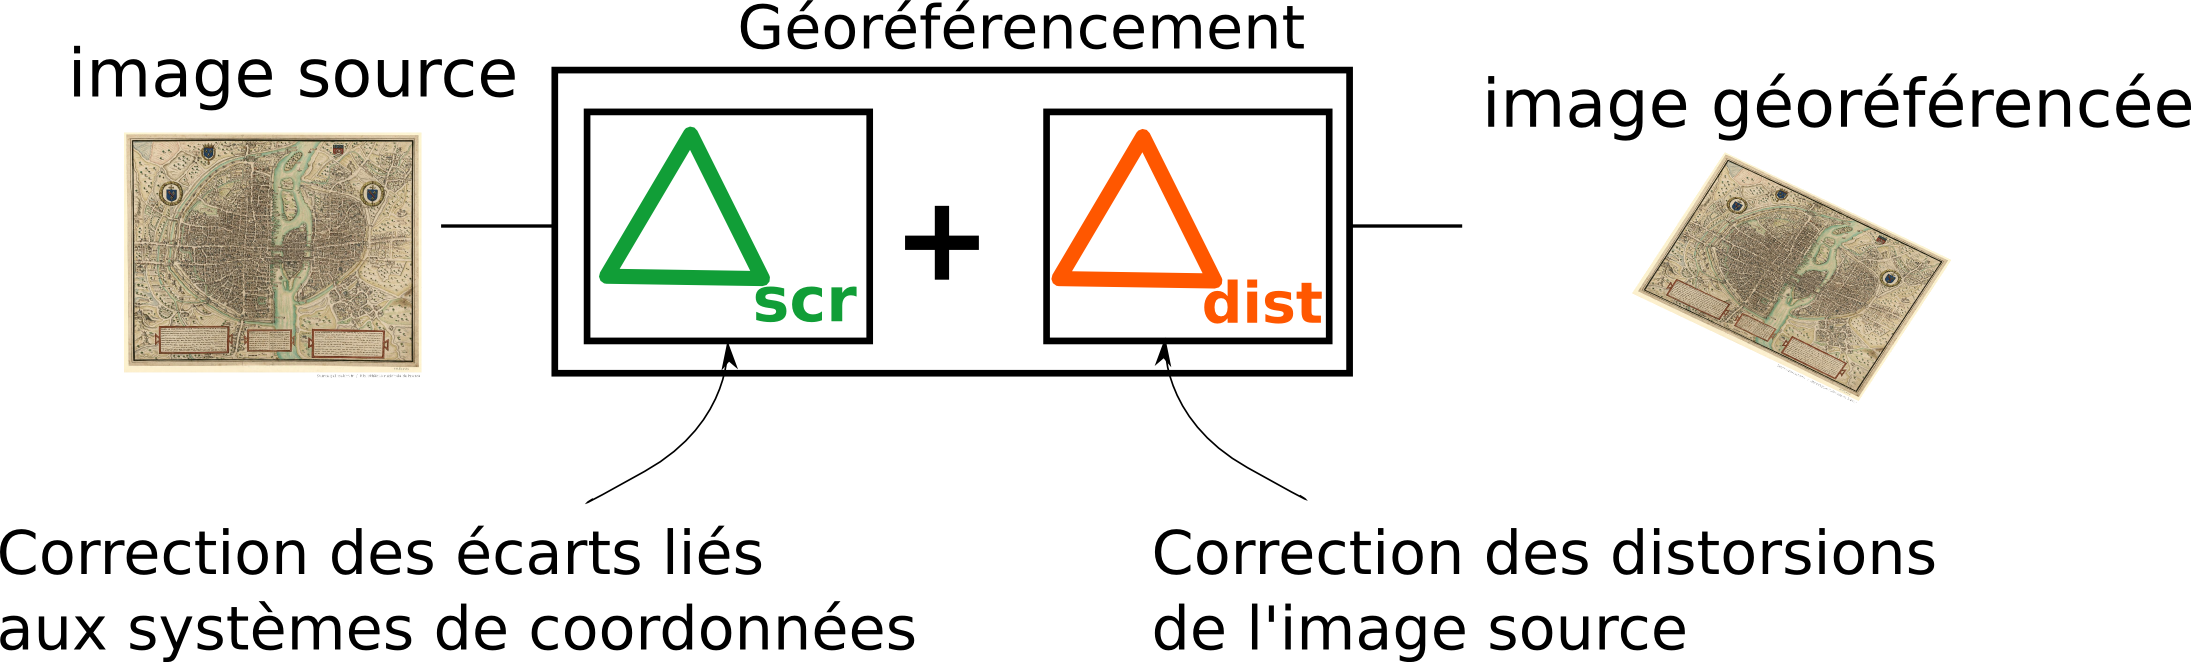
\includegraphics[width=0.7\textwidth]{georef_correction_error.png}
         \caption{Corrections g�om�triques effectu�es lors d'un g�or�f�rencement indirect.}
	\label{figure:georef_correction_error}
\end{figure}
\\
Selon les connaissances sur l'image que l'on veut g�or�f�rencer, trois cas peuvent se pr�senter~:
\begin{enumerate}
 \item Si $F$ est connue \emph{a priori}, sa mod�lisation est possible et applicable directement. Les points d'amer ne sont alors pas n�cessaires. Il s'agit cependant d'un cas th�orique, les param�tres entrant en jeu lors de la cr�ation d'une image � recaler �tant rarement tous ma�tris�s et jamais avec une pr�cision absolue.
 \item Si cette transformation est connue sans qu'il soit possible de la mod�liser directement car incompl�tement ou impr�cis�ment d�finie, l'objectif est alors d'en construire une approximation que l'on ajuste � l'aide d'un ensemble de points d'amer. Cette m�thode est utilis�e notamment pour le g�or�f�rencement direct de photographies a�riennes, pour lequel des points peuvent �tre utilis�s pour am�liorer la pr�cision du mod�le construit � partir des param�tres d'acquisition (cf. le paragraphe \ref{paragraph:direct_georef}).
 \item Dans le cas o� elle est totalement inconnue, on est contraint de choisir arbitrairement un mod�le de transformation qu'il faut ensuite adapter au cas courant.
\end{enumerate}
Dans la suite du propos, nous nous concentrerons sur le troisi�me cas. Pour les cartes anciennes, le mod�le de transformation est toujours inconnu. En effet, m�me si l'on essaye de recomposer le syst�me de projection de la carte ancienne, aucun mod�le caract�ristique des distorsions de celle-ci n'est disponible a priori. 

\myparagraph{Estimation de $F$ dans le cas d'un mod�le de transformation inconnu}
\label{paragraph:leastsquares}
Pour plus de simplicit�, nous nous abstrayons momentan�ment des syst�mes de coordonn�es. Consid�rons simplement deux images, l'une source $I_s$ et l'autre cible $I_c$ sur lesquelle un ensemble $\{(p_1,p'_1),(p_2,p'_2),\dots,(p_n,p'_n) \}, n \in \mathbb{N}$ de points d'amer sont d�finis, o� $p_i $ est dans le rep�re de $I_s$ et $p'_i$ dans le rep�re de $I_c$. On cherche alors une fonction de transformation $F$ quelconque de param�tres $\{\alpha_1, \alpha_2,\dots,\alpha_k\}, k\in \mathbb{N}$ telle que $F(p_i)=p'_i$.
\\
La d�termination de ces param�tres est alors r�alis�e par estimation statistique. Il s'agit de rechercher les param�tres estim�s $\{\hat{\alpha_1}, \hat{\alpha_2}, \dots, \hat{\alpha_k}\}$ qui d�finissent une fonction de transformation $\hat{F}$ telle que  $\hat{F}(p_i) = \hat{p}'_i \approx p'_i$. Cette estimation est usuellement faite par la m�thode des moindres carr�s ordinaires. Il s'agit alors de minimiser \textbf{l'erreur d'estimation} ou \textbf{erreur quadratique moyenne} d�finie par l'�quation \ref{equation:RMSE} (Pour les sources anciennes, $d_2$ est la distance euclidienne entre deux points). La fonction $d_2(p_i,\hat{p}_i)$ est l'\textbf{erreur r�siduelle} pour l'estimation du point $p_i$. La figure~\ref{figure:erreur_estimation} illustre cette erreur d'estimation.
\begin{equation}
RMSE(\hat{F} | F) = \sqrt{\frac{\sum\limits_{i=1}^{n} d_2(p_i,\hat{p}_i)}{n}}
\label{equation:RMSE}
\end{equation}
Pour se replacer dans le cadre du recalage d'image, il s'agit de minimiser $1-RMSE(\hat{F} | F)$. Cette fonction d'erreur est pr�cieuse car elle renseigne sur la qualit� du mod�le estim�, c'est � dire ici de la fonction $\hat{F}$. Nous verrons qu'elle peut �galement servir � analyser la qualit� planim�trique d'une carte ancienne.
\begin{figure}[ht!]
  \centering
        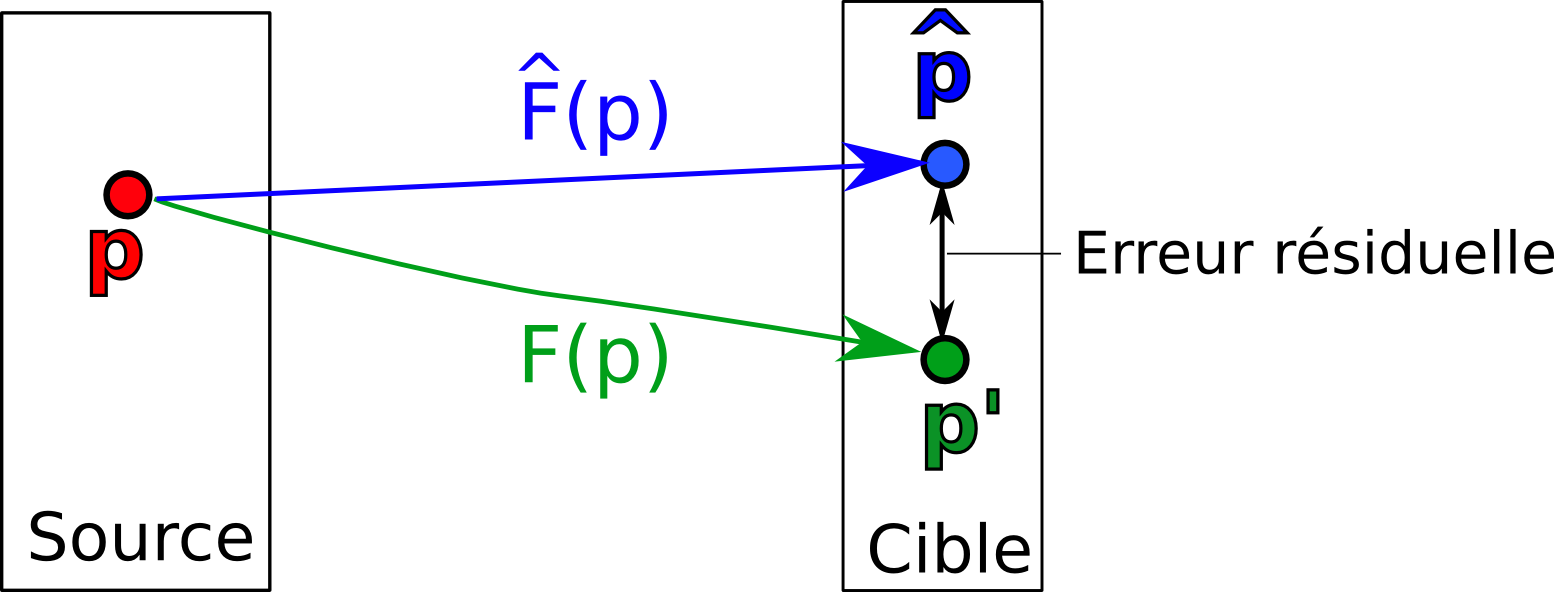
\includegraphics[width=0.5\textwidth]{detail_estimation.png}
         \caption{Illustration de l'erreur r�siduelle dans un cas d'estimation par moindres carr�s ordinaires.}
	\label{figure:erreur_estimation}
\end{figure}
\subsection{Types de fonctions de transformation dans le cas indirect}
\label{subsection:transformations}
Nous sommes rest�s jusqu'ici dans le cadre o� la fonction $F$ n'avait pas de forme d�finie. L'estimation �tant effectu�e par moindres carr�s ordinaires, les param�tres � estimer doivent suivre un mod�le lin�aire, ce qui limite la nature des fonctions utilisables. Nous listons ici trois mod�les de fonctions de transformation utilis�s habituellement dans le cadre du g�or�f�rencement indirect~\citep{Boutoura2006}. Ces m�thodes sont class�es par ordre croissant du nombre de points d'amer n�cessaires � leur estimation. Nous pr�sentons �galement succinctement une autre m�thode n'utilisant pas d'estimateur statistique mais souvent utilis�e pour le g�or�f�rencement et nous jugerons de son adaptabilit� aux cas des cartes anciennes. Notons enfin que r�cemment, des mod�les d'estimation se fondant sur des noyaux gaussiens ont �t� utilis�s avec succ�s pour le g�or�f�rencement de cartes anciennes~\citep{Herrault2013}.
\\
Dans les paragraphes suivants, on notera un point d'amer en 2 dimensions $p=(x,y)$ et nous traiterons de transformations du plan. En effet, notre syst�me source �tant d�j� projet�, nous verrons dans la prochaine section comment choisir un syst�me cible projet� ad�quat aux plans de Paris. En restant continuellement dans un espace en 2 dimensions, les transformations sont plus simples et n�cessitent moins de points d'amer pour �tre estim�es. Toutes ces m�thodes sont dites \textbf{globales}, c'est � dire qu'elles s'appliquent sur la totalit� des points. Cependant, les transformations polynomiales sont des fonctions globales \textbf{� adaptation locale} puisque les termes des polyn�mes permettent de prendre en compte les distorsions locales dans une ensemble de points d'amer.
 
\myparagraph{Transformation de Helmert}
La transformation de Helmert est une similitude utilis�e habituellement en g�od�sie pour effectuer des transformations entre syst�mes de coordonn�es g�ographiques. Elle est d�finie pour le cas g�n�ral de syst�mes g�ographiques en 3 dimension par l'�quation \ref{equation:helmert} et comporte~:
\begin{enumerate}
\item une translation dans chaque direction $C$,
\item un changement d'�chelle $\mu$,
\item une rotation sur chacun des axes x, y et z ($R$);
\end{enumerate}
\begin{equation}
F_{helmert}(x) = C+\mu R x
\label{equation:helmert}
\end{equation}
Dans le cas o� le syst�me source et cible sont tous deux projet�s, il n'y a plus besoin que de 4 param�tres~: 2 translations, une rotation et un changement d'�chelle. Il faut au minimum 2 points d'amer pour estimer une telle transformation.
\paragraph{Transformations affines}
Les transformations affines sont les fonctions de transformation g�om�triques les plus simples. Nous pr�sentons ici la transformation affine � 6 param�tres qui effectue deux translations, deux changements d'�chelle et une rotation.La forme de cette transformation est donn�e par l'�quation~\ref{equation:affine6} et n�cessite au minimum 3 points d'amer.
\begin{equation}
\begin{split}
F_{affine6}(x) = xa+yb+c \\
F_{affine6}(y) = xd+ye+f 
\end{split}
\label{equation:affine6}
\end{equation}
o� $a, b, c, d, e, f$ sont les param�tres de transformation regroupant translation (c,f) ainsi que rotation et changements d'�chelle $(a, b, d, e)$.
\myparagraph{Transformations polynomiales}
Les transformations polynomiales sont de la forme d�crite par l'�quation~\ref{equation:polynome}. Le nombre de points d'amer n�cessaire d�pend du degr� $m$ du polyn�me et est donn� par $\frac{(m+1)(m+2)}{2}$. G�n�ralement, les polynomiales d'ordre 2 et 3 sont utilis�es et n�cessitent respectivement 6 et 10 points d'amer pour �tre estim�es. Des polyn�mes d'ordre plus �lev� peuvent �tre utilis�s, mais la transformation devient alors de plus en plus sensible aux �ventuels points d'amer aberrants dus notamment � des erreurs lors du placement.
\begin{equation}
\begin{split}
F_{poly}(x) = \sum\limits_{i=0}^{m}\sum\limits_{j=0}^{m-1}a_{ij}x^iy^j \\
F_{poly}(y) = \sum\limits_{i=0}^{m}\sum\limits_{j=0}^{m-1}b_{ij}x^iy^j
\end{split}
\label{equation:polynome}
\end{equation}

\myparagraph{Mod�le non lin�aire~: Thin Plate Spline}
La m�thode \emph{Thin Plate Spline} est une m�thode d'interpolation dans laquelle l'objectif est de construire une surface d�form�e de fa�on minimale passant par un ensemble de points. Dans le cas de points d'amer en deux dimensions, il s'agit de d�terminer la fonction $F(a)=a'$ tout en d�formant au minimum la carte source. Cette m�thode pr�sente l'avantage de ne pas reposer sur une estimation statistique et donc ne pas d�pendre d'un nombre de points d'amer minimum (2 suffisent pour cr�er une surface). Cependant, elle fait correspondre exactement les points d'amer de la carte source avec ceux du rep�re cible et est donc particuli�rement sensible aux points d'amer erron�s ou impr�cis. Or les cartes anciennes sont fondamentalement impr�cises, et il est impossible de garantir l'exactitude des points d'amer. De plus, ceux-ci sont g�n�ralement plac�s de fa�on manuelle et donc entach�s d'erreurs de point�~\citep{Girres2012}. Pour cette raison, nous ne consid�rons pas cette m�thode dans la suite de ce travail.

\section{�valuation de la qualit� d'un g�or�f�rencement indirect}
\label{section:qualitygeoref}
Qu'il s'agisse d'identifier des transformations par des mesures ou par la simple superposition de deux cartes, des erreurs dans cette identification peuvent appara�tre lorsque les contenus des cartes sont d�form�s et d�cal�s\footnote{Les objets g�ographiques sont alors distordus et leur localisation erron�e.}. En plus de projeter un plan dans un espace g�ographique, le g�or�f�rencement, puisqu'il transforme l'image, permet de corriger les erreurs planim�triques du plan et donc de ''gommer'' ses distorsions. 
\\
La qualit� d'un g�or�f�rencement se d�finit donc comme sa capacit� � d�terminer une transformation spatiale projetant les points d'amer de la source au plus pr�s de leur correspondant dans le r�f�rentiel cible, et donc corriger les distorsions de la source. De plus, un g�or�f�rencement d�pendant d'un ensemble de points d'amer, sa qualit� repose �galement sur celle de ces points.

\subsection{Exactitude d'un g�or�f�rencement}
Dans le cas des cartes anciennes, les erreurs et les d�formations g�om�triques in�vitablement pr�sentes faussent les distances entre les �l�ments d'un m�me plan comme elles affectent leur positionnement dans l'espace g�ographique du r�f�rentiel. Le risque principal est alors de confondre erreurs de positions et r�els changements des objets repr�sent�s dans la carte ancienne~\citep{Pontius2006}. Lorsque erreurs et diff�rences de repr�sentation se cumulent pour d�former et d�placer deux observations, le risque d'erreur d'identification et de classification d'une transition augmente d'autant plus que les objets repr�sent�s sont denses. Il est donc important que le g�or�f�rencement corrige au mieux les erreurs planim�triques des cartes anciennes. Il s'agit donc de mesurer l'exactitude du g�or�f�rencement, c'est � dire \textbf{le degr� avec lequel il se rapproche de la ''valeur vraie'' - ici l'espace du r�f�rentiel}.
\\
Cette valeur vraie n'est connue qu'au travers des points d'amer, que l'on consid�re fiables dans le rep�re cible. Cette exactitude peut se ramener aux erreurs r�siduelles entre les points d'amer de la source transform�s dans le rep�re cible $\hat{a}_i$ par moindres carr�s et les points $a'_i$ d�finis dans le rep�re cible. On utilise g�n�ralement la RMSE( voir le paragraphe \ref{paragraph:leastsquares}) pour mesurer cette exactitude.
\\
Cette mesure pr�sente l'avantage d'�tre exprim�e dans les m�mes unit�s que les donn�es, facilitant son interpr�tation. Elle est cependant particuli�rement sensible aux erreurs dans les donn�es. En effet, la mise au carr� des erreurs r�siduelles amplifie l'effet d'une mesure aberrante.

\subsection{Qualit� des points d'amer}
Le mod�le de transformation estim�e par moindres carr�s, et donc la pr�cision du g�or�f�rencement, d�pend fortement des points d'amer d�finis. La qualit� d'un ensemble de points d'amer dans la source ou dans le r�f�rentiel cible repose sur trois points~: leur nombre, leur r�partition et leur fiabilit�.

\myparagraph{R�partition spatiale}
L'agencement des points d'amer dans l'espace de la source et de la cible est d'une importance capitale. En effet, une r�partition homog�ne permet de r�duire les erreurs induites par les d�formations locales de la carte lors du calcul des param�tres de transformation. � l'inverse lorsque tous les points sont concentr�s sur une zone de la carte, le mod�le estim� sera juste localement mais d'autant plus fauss� ailleurs que les d�formations locales sont importantes. \cite{Boutoura2006} illustrent parfaitement ce ph�nom�ne en comparant diverses transformations appliqu�es � un sous-ensemble de points d�finis sur une image.
\\
Nous illustrons �galement ce ph�nom�ne en suivant leur m�thode dans les figures~\ref{figure:effets_repartition_1} et \ref{figure:effets_repartition_2} . Nous disposons d'une image source quadrill�e que l'on souhaite projeter dans un r�f�rentiel contenant une version bruit�e al�atoirement de ce quadrillage. Un ensemble de points d'amer est d�fini sur les intersections des lignes du quadrillage, dans la source et dans le r�f�rentiel cible. On applique ensuite un bruit al�atoire aux points du quadrillage dans le r�f�rentiel g�ographique \ref{figure:effets_repartition_1}. Nous appliquons d'abord une transformation rigide -ici de Helmert-utilisant tous les points de contr�le, aboutissant � la grille transform�e en figure \ref{figure:effets_repartition_2_1}. On applique ensuite la m�me transformation � l'image d'origine, cette fois en utilisant uniquement les points 15, 16, 20 et 21, menant � une seconde transformation \ref{figure:effets_repartition_2_2}.
\\
On peut ainsi constater l'importance de la r�partition spatiale des points. Dans la figure \subref{figure:effets_repartition_2_1}, les points r�partis sur toute l'image permettent d'absorber les d�calages locaux dus au bruit. A l'inverse dans la figure \subref{figure:effets_repartition_2_2} seuls quatre points situ�s dans une r�gion r�duite sont utilis�s, aboutissant � une transformation adapt�e � cette zone mais largement d�cal�e pour les autres parties de l'image.

\begin{figure}[ht]
  \centering
        \includegraphics[width=0.8\textwidth]{effets_repartition_spatiale_bruit.png}
         \caption{Illustration des effets de la r�partition des points d'amer~: image source et r�f�rentiel bruit�}
	\label{figure:effets_repartition_1}
\end{figure}


\begin{figure}[ht]
\centering
        \begin{subfigure}[t]{0.4\textwidth}
                \includegraphics[width=\textwidth]{effet_repartition_2.png}
                \caption{...avec tous les points d'amer}
	           \label{figure:effets_repartition_2_1}
        \end{subfigure}%
~
	\begin{subfigure}[t]{0.4\textwidth}
                \includegraphics[width=\textwidth]{effet_repartition_3.png}
                \caption{...avec 4 points regroup�s}
	           \label{figure:effets_repartition_2_2}
	\end{subfigure}%
\caption{Illustration des effets de la r�partition des points d'amer~: application}
\label{figure:effets_repartition_2}
\end{figure}


\myparagraph{Nombre de points}
En plus de leur r�partition, le nombre de points plac�s sur la carte joue �galement un r�le important dans la qualit� d'un g�or�f�rencement~\citep{Boutoura2006}. Tout d'abord, les diff�rents types de transformation en imposent un nombre minimum, n�cessaires pour l'estimation de leurs param�tres. Au del� de cette borne inf�rieure, les nouveaux points d�finis permettent d'am�liorer l'exactitude du g�or�f�rencement pour deux raisons~:
\begin{itemize}
 \item l'approximation du mod�le de transformation est am�lior�e par l'ajout de nouvelles connaissances,
  \item la r�gression lin�aire utilis�e pour d�terminer les param�tres des transformation moyenne les erreurs, ce qui permet d'absorber les d�formations locales.
\end{itemize}
Cependant, il n'est pas toujours souhaitable d'augmenter ce nombre au del� d'un certain seuil.
Dans la figure \ref{fig:nb_pts_herrault} issue des r�sultats pr�sent�s dans le travail de \cite{Herrault2013}, on constate cependant que pour les deux distributions, le gain de pr�cision devient nul d�s 100 points plac�s. Une telle stagnation signifie que le g�or�f�rencement le plus pr�cis, �tant donn� la pr�cision relative du r�f�rentiel et de la carte ancienne, a �t� atteint. � partir de ce moment l�, l'ajout de nouveaux points devient risqu� puisque qu'il peut entra�ner une d�gradation de la qualit� du g�or�f�rencement. Cette constatation n'est cependant vraie que pour les transformations globales sans effet local (similitudes, affines, projectives) puisque les erreurs locales moyenn�es se retrouvent distribu�es sur l'ensemble de la carte.
\\
Le m�me auteur trace �galement un lien entre le nombre de points et leur r�partition, le choix de l'un d�pendant de l'autre. Ainsi, lorsqu'un grand nombre de points est disponible, une r�partition al�atoire tend � donner un meilleur g�or�f�rencement. Inversement lorsque les rep�res sont faibles, une r�partition r�guli�re donne de meilleurs r�sultats. Ce ph�nom�ne s'explique~: de nombreux points r�partis al�atoirement vont mieux ''couvrir'' la carte qu'un faible nombre r�partis de mani�re similaire qui laissent des zones ''vides''. 
\\
\textbf{La r�gle est donc la suivante~: moins on dispose de points, plus il doivent �tre r�partis de fa�on homog�ne et r�guli�re sur la carte.}

\begin{figure}[ht]
\centering 
\includegraphics[width=\textwidth]{herrault2.png}
\caption{�volution de l'erreur r�siduelle sur un �chantillon de la ''Carte de France'', ici exprim�e par l'Erreur Quadratique Moyenne r�siduelle (RMSE) suivant diff�rents mod�les de transformation globale utilis�s dans cette th�se et pour diff�rents types de r�partition de points d'amer. D'apr�s les donn�es issues de \citep[p.41]{Herrault2013}.}
\label{fig:nb_pts_herrault}
\end{figure}

\myparagraph{Fiabilit� des points}
� notre connaissance, la fiabilit� d'un point d'appui n'a pas fait l'objet d'une d�finition claire parmi les diff�rents travaux. 
Dans le domaine de la photogramm�trie, il s'agit g�n�ralement de recaler dans un rep�re g�ographique des images satellitaires ou a�riennes � l'aide de relev�s GPS. La fiabilit� est alors directement li�e � la pr�cision planim�trique des points \citep{Gregory2005}.
\\
Puisque dans notre cas les points sont plac�s manuellement, on doit �galement consid�rer l'impr�cision de placement ou \textit{erreur de point�}\citep[p.162]{Girres2012}. Il s'agit de l'erreur accidentelle de positionnement du point r�sultant du processus et du choix de l'�chelle de saisie~: un utilisateur humain muni d'un outil de point� (souris,etc.) va n�cessairement introduire une erreur de positionnement.
\\
Lorsqu'il s'agit de donn�es incertaines comme le sont les cartes anciennes, il faut �galement s'interroger sur la confiance port�e aux informations qui y sont d�crites. En effet, si l'on place des points sur des objets cartographiques consid�r�s comme ''inchang�s'', encore faut-il �tre certain qu'ils le soient effectivement~\citep{Benavides2006}. Si cette question est secondaire pour des images satellite o� le r�f�rentiel (la r�alit�) est disponible, elle l'est moins pour des objets historiques dont la localisation peut avoir chang� sans que leur forme globale n'ait �t� modifi�e\footnote{Un des meilleurs exemple est sans doute la reconstruction de b�timents incendi�s, r�guli�rement -du moins � Paris- modifi�e par rapport � l'original malgr� une certaine volont� de reproduire l'�difice ''� l'identique''. Citons par exemple le th��tre du Panth�on ou encore la Bourse du Commerce.}, ou lorsque l'�cart temporel entre l'objet dans la carte ancienne et celui dans le r�f�rentiel est tel qu'il devient difficile de se prononcer sur sa stabilit�. Les diff�rences de repr�sentation entre la carte et le r�f�rentiel, les niveaux de g�n�ralisation de chacun ou encore la r�solution spatiale de la carte agissent aussi sur le degr� de confiance attribu� � un point~: plus la carte est �loign�e (en termes de repr�sentation) du r�f�rentiel, moins le point sera fiable. \cite{Zanola2009} a d�montr� cet effet sur des donn�es 3D st�r�oscopiques, le niveau de photo-r�alisme d'un objet 3D influant fortement sur le degr� de confiance des utilisateurs dans la qualit� de ces donn�es.
\\
Finalement, la notion de fiabilit� est dans notre cas caract�ris�e par deux �l�ments~:
\begin{itemize}
 \item la pr�cision planim�trique des points, d�pendant de la pr�cision de la carte, de celle du r�f�rentiel, de l'�chelle et du processus de saisie,
 \item le niveau de confiance attribu� � une correspondance entre un objet de la carte et un objet du r�f�rentiel.
\end{itemize}



\section[G�or�f�rencement des plans de Paris]{Proposition~: une m�thode de g�or�f�rencement adapt�e aux plans topographiques anciens de Paris}
\label{section:proposition}
Dans la section \ref{section:georef_global}, nous avons pr�sent� les �l�ments n�cessaires pour effectuer un g�or�f�rencement indirect. En particulier, lorsque l'on dispose d'une image -carte, plan, etc.- � g�or�f�rencer, cinq param�tres doivent �tre d�termin�s~:
\begin{itemize}
\item le syst�me de coordonn�es de la source,
\item le syst�me de coordonn�es cible,
\item un r�f�rentiel g�ographique sur lequel placer des points d'amer,
\item un ensemble de points d'amer dans la source et leurs correspondants dans le r�f�rentiel,
\item une transformation spatiale;
\end{itemize}
Dans cette section, nous proposons de fixer ces diff�rents param�tres pour le cas des plans topographiques parisiens. Nous montrons notamment que l'on peut d�terminer un syst�me de projection commun pour la source et la cible, ce qui nous permet de nous abstraire des erreurs de g�or�f�rencement dues aux changements de syst�mes de coordonn�es et ainsi nous focaliser sur l'analyse des distorsions des plans anciens.


\subsection{Choix du syst�me de projection des plans topographiques anciens de Paris}
En pr�sentant le g�or�f�rencement indirect, nous avons pr�cis� qu'il �tait tout � fait envisageable de g�or�f�rencer une image -ici une carte ancienne- sans connaissances pr�alables sur son syst�me de projection. Nous avons �galement montr� que dans ce cas pr�cis, la fonction de transformation spatiale m�lait � la fois la projection de l'image dans le rep�re cible et les corrections de ses distorsions.
\\
Il est pourtant particuli�rement int�ressant, lorsque l'on traite de cartes anciennes, d'�tre capable d'analyser leurs distorsions~\citep{Jenny2011}. Or il n'est possible de les isoler que si l'on connait le syst�me de projection de la source, ce qui permet de s�parer des distorsions dues aux erreurs de la carte de celles dues � l'�cart entre son syst�me de projection et celui du r�f�rentiel cible.
\\
Nous pr�sentons dans cette section la m�thode que nous avons adopt� pour d�terminer le syst�me de projection de nos plans topographiques anciens.

\myparagraph{Probl�mes introduits par les cartes historiques}
Nous avons pr�sent� les �l�ments requis pour projeter un espace g�ographique.
%Dans notre cas nous souhaitons transformer un plan ancien dans un syst�me de coordonn�es connu de fa�on � rassembler les donn�es dans un m�me espace mais aussi de faciliter l'interop�rabilit� avec d'autres donn�es g�ographiques \footnote{En effet, tous les outils SIG actuels permettent, ais�ment, de projeter un ensemble de donn�es d'un syst�me de coordonn�es � un autre.}. Il s'agit donc d'un cas particulier de changement de syst�mes, pour lequel celui des donn�es anciennes doit �tre retrouv�.
Nous avons dit que la recomposition d'un syst�me ancien est difficile, en raison surtout du manque de documentations sur la construction m�me de la carte. Si pour celle de Cassini le syst�me de projection a pu �tre recompos� gr�ce aux calculs de la m�ridienne de Paris, retranscrits avec forts d�tails dans les livres �dit�s par Cassini de Thury (voir les travaux de \cite{Berthaut1898}), il s'agit plut�t d'une exception pour la p�riode \footnote{On trouve le d�tail du syst�me de coordonn�es sur le site du projet de reconstitution et de gor�f�rencement de la carte de Cassini~: \url{http://cassini.ehess.fr/cassini/fr/html/5_donnees.htm}. A partir du XIX\up{e} si�cle, la projection de Cassini (ou Cassini-Soldner) sera plus g�n�ralement utilis�e.}. Notons toutefois que l'atlas de Verniquet est �galement extr�mement bien document� puisqu'une somme importante des minutes des lev�s topographiques du plan ont �t� retrouv�s et se trouvent aujourd'hui � la Biblioth�que Historique de la Ville de Paris (BHVP). La reconstitution de la triangulation de l'atlas � partir de ces minutes serait d'un aide pr�cieuse, que nous n'avons pas trait� en raison du volume de donn�es et de leur difficult�\footnote{Il s'agit, en d�tails, de tous les calculs et trac�s des triangles et chemins polygonaux dans les rues de Paris. Pour reconstituer le canevas de l'atlas, il faut donc reproduire le travail de l'�quipe d'Edm� Verniquet et replacer tous ces trac�s par rapport aux triangles principaux puis � la m�ridienne.}.

\myparagraph{Projections des plans de Paris}
La cartographie urbaine s'est dot�e de syst�mes locaux construits par triangulation � partir de m�ridiens situ�s � proximit�.
En France et � Paris, le m�ridien d'origine passant � l'Observatoire Royal a �t� utilis� d�s sa d�termination par Cassini en 1683. Cependant, sa position exacte a �t� corrig�e r�guli�rement, la d�pla�ant l�g�rement � chaque fois. Deux calculs ont fait autorit� pendant notre p�riode~:
\begin{itemize}
 \item celui de Delambre et M�chain effectu� dans les derni�res ann�es du XVIII\up{e} si�cle;
 \item la \textit{nouvelle m�ridienne de France} en 1893.
\end{itemize}
Pour Paris, tous les plans sur lesquels nous travaillons ont �t� construits � partir d'une triangulation fond�e sur le m�ridien de Paris, sauf -sans certitude aucune- le plan de Maire qui s'appuie sur un travail ant�rieur � la d�termination du m�ridien.
De plus, Paris se trouve tr�s exactement sur le trac� du m�ridien puisqu'il passe au travers de l'observatoire aujourd'hui situ� dans le XIV\up{e} arrondissement.
Bien que nous ne connaissions pas en d�tail les m�thodes de construction de chacun des plans, ceux-ci se trouvent tr�s proches du m�ridien d'origine, parfaitement connu � l'�poque.
\\
Deux possibilit�s s'offrent � nous~:
\begin{itemize}
\item si l'on est capable de reconstituer la triangulation du plan et que l'on connait la position du m�ridien de Paris, on peut alors recr�er le syst�me de projection ancien,
\item on peut essayer d'approximer le syst�me ancien par un syst�me projet� de r�f�rence dont l'alt�ration lin�aire sur la zone peut �tre consid�r�e n�gligeable �tant donn� les imperfections inh�rentes aux cartes ancienne.
\end{itemize}
Nous allons voir qu'� Paris, la seconde solution est envisageable.

\myparagraph{Approximation du syst�me de projection des plans de Paris par un syst�me de projection de r�f�rence}
Le choix d'un syst�me de coordonn�es ad�quat d�pend, on l'a vu, de la zone g�ographique couverte. En France, la mise en place du syst�me g�od�sique de r�f�rence RGF93 (R�seau G�od�sique Fran�ais) a �t� accompagn�e par la d�finition d'une nouvelle projection cartographique nomm�e Lambert 93. S'appuyant sur l'ellipso�de IAG-GRS80, il s'agit d'une projection conique conforme dont le m�ridien d'origine est Greenwich, adopt�e depuis 2000 comme projection cartographique officielle pour la France m�tropolitaine. Pr�c�demment � ce syst�me existait, pour le m�me territoire, un ensemble de quatre projections fond�es sur l'ancien syst�me g�od�sique de r�f�rence NTF (Nouvelle Triangulation de la France) cr��e au XIX\up{e} si�cle. Les projections Lambert I, II et III couvraient ainsi la France continentale tandis que le Lambert IV avait �t� mis en place pour la Corse. La figure \ref{figure:lamberts} pr�sente les grilles de projection des quatre zones Lambert NTF et du Lambert 93 \citep{DOC_GEODESIE2}.
\begin{figure}[ht!]
  \centering
        \includegraphics[width=0.4\textwidth]{lamberts.png}
         \caption{Zones Lambert I, II, III et IV. Figure issue de documents IGN.}
	\label{figure:lamberts}
\end{figure}
L'objectif est donc de choisir parmi ces diff�rents syst�mes de projection celui qui pr�sente le moins d'alt�rations lin�aires\footnote{L'alt�ration lin�aire est l'�cart existant entre par une longueur mesur�e en projection et la m�me longueur mesur�e sur l'ellipso�de de r�f�rence.} au niveau de Paris. La figure~\ref{fig:lambertsvs} montre l'�volution de ces alt�rations selon la latitude. On constate que les projections Lambert I et Lambert 93 pr�sentent des alt�rations faibles au niveau de Paris, inf�rieures au m�tre. Afin de v�rifier ces alt�rations, nous avons calcul� l'alt�ration lin�aire de la borne g�od�sique situ�e sur le pilier de la m�ridienne de France\footnote{Fiche g�od�sique IGN 75056A, point A. \url{http://geodesie.ign.fr/fiches}} en projetant les coordonn�es g�ographiques (RGF93) de la borne dans les syst�mes Lambert. Ces mesures ont �t� effectu�es avec le logiciel Circ� France de l'IGN\footnote{\url{http://geodesie.ign.fr/index.php?page=circe}}. Pour le Lambert I, nous avons obtenu une alt�ration d'environ 6 centim�tres par kilom�tres\footnote{La longueur de Paris est aujourd'hui de 18 kilom�tres de l'est � l'ouest en comptant les bois de Boulogne et Vincennes, et de 9,5 kilom�tres du nord au sud.}. Pour le Lambert 93, nous avons mesur� une alt�ration d'environ 12 centim�tres.
\begin{figure}[ht!]
  \centering
        \includegraphics[width=0.8\textwidth]{alterations.png}
         \caption{Comparatif des alt�rations lin�aires des lambert I, II, III, IV et Lambert 93. La latitude de Paris est d'environ $48,8$ degr�s d�cimaux. Figure issue de documents IGN.}
	\label{fig:lambertsvs}
\end{figure}
\paragraph{}
Au del� de l'alt�ration lin�aire, le m�ridien d'origine est �galement � prendre en compte. En effet, les deux projections sont directes, c'est � dire qu'elles sont orient�es nord-sud suivant un m�ridien d'origine. Nos plans pr�sentent presque tous des carroyages align�s sur le m�ridien de Paris, il est donc plus simple de consid�rer le cas o� le m�ridien de Paris se trouve vertical. Pour ces deux raisons, nous utilisons la projection Lambert I comme approximation des syst�mes de coordonn�es projet� de nos plans topographiques. Ajoutons que depuis 2006, neuf nouvelles projections coniques conformes ont �t� d�finies sur le territoire (nomm�es Lambert CC 42 � 50) r�duisant l'alt�ration  lin�aire � l'intervalle $[-9cm;+7cm]$ afin de palier les alt�rations relativement importantes de la projection Lambert 93. � Paris, il s'agit du Lambert CC49, qui pr�sente une alt�ration lin�aire de 8 centim�tres~\citep{DOC_GEODESIE1}.

\subsection{Choix du syst�me de projection du r�f�rentiel g�ographique cible}
Le choix d'un syst�me de coordonn�es pour le r�f�rentiel g�ographique est n�cessaire pour effectuer un g�or�f�rencement.
En choisissant le Lambert I NTF comme syst�me de coordonn�es projet�es des plans topographiques de Paris, nous avons d�j� la possibilit�, lors du g�or�f�rencement, de s�parer les �carts dus aux diff�rences entre les syst�mes de coordonn�es source et cible d�s lors que ce dernier est un syst�me de coordonn�es de r�f�rence. En effet, les fonctions de passage entre le Lambert I NTF et ce syst�me sont connues.
\\
Plus encore, le fait d'avoir consid�r� que le syst�me de projection des plans de Paris pouvaient �tre approxim� par le Lambert I NTF nous permet de choisir le m�me syst�me projet� pour le r�f�rentiel cible. Ainsi, sous l'hypoth�se que le Lambert I est une bonne approximation du syst�me de projection des plans de Paris, nous �liminons les �carts dus � un changement de syst�me lors du g�or�f�rencement(voir la section~\ref{section:verifications}). De cette fa�on, nous pouvons nous concentrer uniquement sur l'analyse des distorsions des plans anciens de Paris.
\\
Sur nos plans de Paris, l'�chelle est toujours indiqu�e dans le cadre ou le cartouche du plan, ce qui permet de transformer simplement les points d'amer plac�s dans l'image dans le syst�me Lambert I. Il s'agit alors d'une simple mise � l'�chelle. 

\subsection{R�f�rentiels g�ographiques actuels utilisables pour le placement des points d'amer}
Nous avons donc choisi un syst�me de projection commun source-cible adapt� aux plans parisiens. L'op�ration implique le choix d'un r�f�rentiel g�ographique, une repr�sentation d'un espace commun aux donn�es anciennes dont on conna�t, pour chaque �l�ment qui la compose, la position � la surface de la Terre avec pr�cision~\citep{Tucci2010}. G�n�ralement, des donn�es g�ographiques r�centes jouent ce r�le~: photographies a�riennes \citep{Brovelli2012, Guerra2000}, bases de donn�es provenant de producteurs nationaux~\citep{Plumejeaud2012} ou de projets collaboratifs~\citep{DaiPra2013}.
\\
Pour obtenir un r�f�rentiel g�ographique utilisable pour les g�or�f�rencer il est encore n�cessaire de choisir un ensemble de donn�es qui serviront � placer des points d'amer. � Paris, de nombreux supports peuvent fournir de telles donn�es sous des formes diverses~: images a�riennes, bases de donn�es vecteurs ou encore cartes. Il est bien s�r possible d'utiliser plusieurs d'entre eux simultan�ment � la condition que tous les plans soient recal�s en utilisant les m�mes donn�es de r�f�rence de fa�on � conserver une pr�cision des donn�es homog�ne.

\myparagraph{Caract�ristiques requises}
Plusieurs �l�ments permettent de choisir un ensemble de donn�es g�ographiques de r�f�rence. Le crit�re principal allie certainement pr�cision planim�trique des donn�es et fiabilit� de l'information repr�sent�e, qui d�pendent surtout du statut du producteur de donn�es. Ainsi en France, l'IGN, producteur officiel des bases de donn�es de r�f�rence � l'�chelle nationale doit respecter un degr� de qualit� et de pr�cision d�fini par son statut.
Ensuite, il est n�cessaire de s�lectionner des donn�es repr�sentant les m�mes objets que les cartes en suivant des r�gles de repr�sentations proches. En effet, le placement pr�cis des points d'amer n'est possible que si les deux objets ne pr�sentent pas de diff�rences de g�n�ralisation et de symbolisation trop importantes. Cela induit �galement la ma�trise des donn�es utilis�es et en particulier des sp�cifications de leurs saisies. Celles-ci forment des m�tadonn�es qui doivent �tre diffus�es en m�me temps que les donn�es elles-m�mes.
Parmi les classes d'objets g�ographiques communes � tous nos atlas parisiens, les b�timents et les rues sont les deux plus significatives. De plus, nous avons �voqu� dans le premier chapitre comment la trace de b�timents disparus pouvaient perdurer au travers des d�coupages parcellaires. Il est donc important que le r�f�rentiel choisi repr�sente ces trois �l�ments.
Dans ce but, nous allons donc pr�senter les bases de donn�es g�ographiques les plus pertinentes, dont des extraits sont visibles dans la figure~\ref{figure:extraits_maps} et en choisir une qui respecte le mieux les points abord�s.
\begin{figure}[ht!]
\includegraphics[width=1\textwidth]{donnes_possibles.png}
                \caption{R�ferentiels g�ographiques envisag�s.}
                \label{figure:extraits_maps} 
\end{figure}
\myparagraph{Plan cadastral fran�ais}
La Direction G�n�rale des Finances Publiques (DGFiP) assure, dans le cadre de ses missions juridiques et techniques, la mise � jour du plan cadastral couvrant le territoire national afin d'identifier, de localiser et de repr�senter les propri�t�s fonci�res. Sous forme papier jusqu'en 2002, le cadastre a �t� presque enti�rement num�ris� puis vectoris� pour former le Plan Cadastral Informatis� (PCI Vecteur). Les feuilles uniquement scann�es forment quant � elles le PCI Image. Le cadastre vecteur a conserv� la forme des feuilles du plan ancien. Il existe donc une base vecteur par commune, divis�e en sections, elles-m�mes form�es � partir de plusieurs sous-sections nomm�es \textit{feuilles de plan}, soit au total 597 179 feuilles. Chacune de ces sections est d�limit�e par des objets g�ographiques relativement stables~: cours d'eau, routes, voies de chemin de fer, etc. Le cadastre fran�ais dessine l'unit� fiscale de base~: la parcelle cadastrale.
Parmi les plans cadastraux des communes, on distingue les plans \textit{mis � jour}, r�alis�s � partir des plans napol�oniens, dont l'�chelle varie entre le 1/1250\up{e} et le 1/5000\up{e}, et les plans dits \textit{r�guliers} construits sur de nouvelles bases\footnote{Les m�tadonn�es du plan cadastral ont �t� diffus�es par le portail G�oBretagne. Voir \url{http://cms.geobretagne.fr/content/fiche-de-m�tadonn�es-type-pour-le-plan-cadastral}}.
Puisque le cadastre a �t� confectionn� � partir d'anciens plans, il a d� �tre lui-m�me r�f�renc� � partir des cartes au 1/25000\up{e} de l'IGN ainsi qu'a l'aide d'orthophotographies. Afin d'assurer, malgr� ces particularit�s, une pr�cision planim�trique suffisante pour �tre utilisable dans un cadre professionnel (chantiers de constructions par exemple), chaque feuille de plan s'est vu assigner une \textit{classe de pr�cision planim�trique}. Elle correspond � l'�cart en centim�tres entre les coordonn�es transform�es par g�or�f�rencement indirect des feuilles et celui observ� en les recalant avec une transformation affine associant une rotation et une translation. Chaque mesure de pr�cision est ensuite adapt�e d'apr�s la pr�cision de la base de donn�es g�ographique de r�f�rence utilis�e pour le g�or�f�rencement. Ainsi, la classe de pr�cision finale retranscrit l'exactitude de la feuille par rapport au r�f�rentiel IGN (cartes et orthophotographie) et non plus uniquement un �cart interne. Le cadastre de Paris, au 1/500\up{e}, a ainsi une classe de pr�cision de 20 centim�tres \footnote{Pour plus de d�tails sur la d�termination des classes de pr�cision, voir \url{http://bofip.impots.gouv.fr/bofip/5195-PGP}} . Il n'existe cependant pas encore de m�tadonn�es d�taill�es pour chaque feuille cadastrale.

\myparagraph{Plan parcellaire de la ville de Paris}
La plan parcellaire de Paris, maintenu par la Direction de l'Urbanisme de la ville de Paris, couvre l'int�gralit� de la capitale � l'�chelle du 1/500\up{e}. Outre les parcelles, il repr�sente �galement les limites administratives, les b�timents et cours, les am�nagements des espaces non b�tis (trottoirs, voies, escaliers, etc.) les adresses et les noms de rues et d'�quipements. Le plan, diffus� en raster, vise une description extr�mement pr�cise des structures urbaines; il distingue par exemple  les murs mitoyens des murs simples ou accol�s pour chaque b�timent. Tout comme le cadastre fran�ais, il s'agit d'un plan num�ris� � partir des anciennes minutes de la Ville et d�sormais mis � jour seulement dans sa version num�rique. La pr�cision planim�trique du plan varie entre 10  et 20 centim�tres, mais peut �tre localement plus importante selon l'�poque du lev� topographique \citep[p. 7]{PARCELLAIRE_PARIS}. 
%Enfin, puisqu'il s'agit d'une image num�ris�e, sa r�solution est importante~: un pixel correspond � 4,2 centim�tres sur le terrain.

\myparagraph{Bases de donn�e l'APUR}
L'Atelier Parisien de l'Urbanisme est une agence regroupant divers acteurs publics d'�le de France  -collectivit�s locales, �tablissements publics, �tat fran�ais- dont l'objectif est d'aider � la mise en place des politiques publiques urbaines par la production de divers documents d'urbanisme. En particulier, cette agence produit des bases de donn�es g�ographiques sur la ville, notamment sur les parcelles cadastrales, les b�timents et les voies de circulation. Les donn�es cr��es par l'APUR sont issues des divers acteurs qui la composent, notamment, pour les parcelles et les voies, la mairie de Paris et la DGFiP, mais ne sont pas pour autant diffus�es librement ou gratuitement. En particulier, les parcelles cadastrales ne sont utilisables que par les �tablissements associ�s � l'agence d'urbanisme. La pr�cision des donn�es APUR n'est cependant pas disponible bien que chaque couche diffus�e soit accompagn�e d'une s�rie de m�tadonn�es d�crivant notamment ses sp�cifications de saisie \footnote{Accessibles sur le G�oportail INSPIRE~: \url{http://inspire-geoportal.ec.europa.eu/discovery/}}.

\myparagraph{Bases de donn�es IGN}
L'IGN propose, au sein du RGE\textregistered (R�f�rentiel � Grande �chelle), un ensemble de bases de donn�es d�crivant le territoire fran�ais. Parmi celles-ci, la BDParcellaire\textregistered~est une version du cadastre fran�ais mise en coh�rence avec les autres donn�es produites par l'�tablissement. Ainsi, les g�om�tries sont corrig�es et toutes les feuilles cadastrales sont rassembl�es en une base de donn�es unique. La BDParcellaire se pr�sente sous une forme raster (c'est alors une version assembl�e du PCI Image) et sous forme vecteur (cr��e � partir du PCI Vecteur). Outre le fait de ne plus morceler le cadastre, ces bases de donn�es pr�sentent l'avantage certain de disposer d'une somme de m�tadonn�es cons�quente renseignant tout le protocole de saisie ainsi que les informations de pr�cision des donn�es. Puisque les g�om�tries sont recal�es par rapport aux autres donn�es du RGE, la pr�cision planim�trique de la BDParcellaire est moindre que celle du cadastre et varie entre 0,5 m�tres et 5 m�tres. � Paris, elle est de l'ordre de 0.5 m�tres. Enfin, elle contient, en plus des parcelles, une couche donnant le d�tail de toutes les surfaces b�ties.

\myparagraph{OpenStreetMap}
L'initiative Open-Source OpenStreetMap vise � cr�er, mettre � jour et diffuser librement une base de donn�es g�ographique vecteur sur la plan�te enti�re. La constitution de cette base est enti�rement fond�e sur un mod�le collaboratif, chacun (�tablissement public ou priv�, particulier) pouvant contribuer de fa�on libre. La r�utilisation des donn�es est libre, mais diffus�es sous la licence contaminante ODbL, obligeant donc toute donn�e d�riv�e � adopter la m�me licence. Depuis 2009, OpenStreetMap int�gre une version du PCI vecteur, mettant donc � disposition les g�om�triques de tout le parcellaire fran�ais. Contrairement aux producteurs de donn�es officiels, le mode de mise � jour d'OpenStreetMap n'assure pas une couverture homog�ne du territoire. Le statut de capitale de Paris lui assure cependant une description tr�s d�taill�e et une fr�quence �lev�e de mises � jour. De plus, pour assouplir la saisie des objets par le grand public, un mod�le de donn�e tr�s l�che a �t� adopt�, sans aucune sp�cification de saisie stricte. La pr�cision des donn�es issues des saisies collaboratives est donc particuli�rement instable.

\myparagraph{BDORTHO\textregistered~IGN}
Dernier r�f�rentiel envisageable, les photographies a�riennes comptent parmi les supports r�guliers du g�or�f�rencement de cartes historiques. Sur Paris, l'IGN met � disposition de fa�on libre, sous forme de flux WMS \footnote{Web Map Service, protocole permettant d'afficher dans un SIG des cartes g�or�f�renc�es provenant de serveurs de donn�es distants. Ici, il s'agit du G�oportail \url{http://www.geoportail.gouv.fr/}} ou d'images g�or�f�renc�es, la mosa�que compl�te de la France � une r�solution de 50 centim�tres. La pr�cision planim�trique quant � elle d�pend de la pr�cision du mod�le num�rique de terrain sur lequel sont g�or�f�renc�es les images. Mais, sur la zone de Paris, elle reste constante � 1 m�tre plus ou moins 50 centim�tres \citep[p. 9]{BDORTHO}.

\myparagraph{S�lection des donn�es de r�f�rence.}
L'utilisation du plan cadastral n'est pas envisageable pour plusieurs raisons. Si son usage est libre pour tout acteur priv� ou public, individuel ou non, sa rediffusion est restrictive (elle est interdite pour les particuliers). En raison de la nature fiscale du cadastre dans lequel la mesure d'aire est cruciale, les parcelles sont aplanies pour conserver leur aire r�elle malgr� la projection plane du plan. Le relief est totalement absent, ce qui entra�ne des d�calages qui peuvent �tre importants dans les zones particuli�rement accident�es. 
%Signalons enfin �galement que les feuilles, issues de plans relativement anciens, ne correspondent pas entre elles~: leur mise en commun induit dont des d�formations suppl�mentaires.
La BDParcellaire\textregistered pr�sente l'avantage d'�tre plus fournie en m�tadonn�es que le cadastre, et, surtout, d'�tre une version fusionn�e de celui ci au prix, cependant, d'une perte de pr�cision. Une fusion de la BDParcellaire\textregistered et du cadastre en une base unique est pr�vue mais n'est pas, actuellement, mise en place. Cette base de donn�es est cependant moins d�taill�e que les plans parcellaires de Paris et de l'APUR.
Ces deux plans constituent les sources de donn�es les plus d�taill�es dont on dispose sur Paris. Si le plan parcellaire de la ville de Paris est en partie mis � jour, en particulier pour les parcelles, � partir des donn�es issues du d�pouillement des feuilles cadastrales par l'APUR, lui seul est disponible librement et gratuitement. En outre, son niveau de d�tail et les objets g�ographiques repr�sent�s correspondent parfaitement � nos demandes~: les b�timents, parcelles et rues sont pr�sentes; le plan est � tr�s grande �chelle; les sp�cifications de saisie sont connues et disponibles \footnote{Voir \href{http://paris-a-la-carte-version-pl.paris.fr/carto/licences/20080206_licence_plan_parcellaire.pdf}{http://paris-a-la-carte-version-pl.paris.fr}}; sa pr�cision th�orique globale est de 10 � 20 centim�tres.
Enfin, nous n'avons pas retenu l'utilisation des photographies a�riennes pour deux raisons. D'une part, la nature m�me des prises de vues a�riennes ne permet pas d'obtenir, partout, une prise de vue � la verticale parfaite du sol. Malgr� une �tape de correction g�om�trique syst�matique, ces images obliques sont difficiles � comparer avec des plans, eux, parfaitement verticaux et, de plus, g�n�rent des zones d'occlusion (arri�re des immeubles �lev�s, reliefs abrupts, etc.). Les parcelles y sont de plus absentes, r�duisant les possibilit�s de placement de points d'amer. Enfin la pr�sence du mobilier urbain, de v�hicules ou de couverture v�g�tale g�ne �galement l'identification de ces points.
\textbf{Nous avons donc choisi de nous appuyer sur le plan parcellaire de la ville de Paris}. En effet, son niveau de d�tail, son �chelle et sa pr�cision en font le meilleur candidat pour g�or�f�rencer des plans � l'�chelle de la ville. Il repr�sente de plus tous les objets communs aux atlas parisiens, ce qui permet de maximiser le nombre d'objets pouvant servir de points d'amer.

\subsection{Choix des points d'amer et des mod�les de transformation spatiale}
\myparagraph{Types d'objets g�ographiques pertinents}
Les points d'amer doivent �tre plac�s sur des objets g�ographiques communs au r�f�rentiel et � la carte ancienne. Deux cat�gories d'�l�ments sont consid�r�s ici~:
\begin{itemize}
\item les objets g�ographiques pr�sents dans la repr�sentation de la carte ancienne et sa repr�sentation actuelle,
\item les �l�ments g�od�siques li�s � la construction du plan tels que son carroyage, la m�ridienne de France et sa perpendiculaire.
\end{itemize}
Afin de permettre la comparaison des distorsions de chacun des plans anciens, il est utile de regrouper les points d'amer selon la nature des objets g�ographiques sur lesquels ils sont plac�s\citep{Grosso2010}. Ainsi, l'interpr�tation des erreurs r�siduelles est plus ais�e. De plus, cela peut permettra d'analyser les diff�rents th�mes cartographiques qui composent la carte.
\\
Les plans dont nous disposons sont pour la majorit� (Verniquet, Jacoubet, Maire, Poubelle) tr�s �pur�s. Les seuls types d'objets g�ographiques que l'on retrouve sur chacun d'eux sont~:
\begin{itemize}
\item les b�timents publics et religieux,
\item les rues, cours et jardins,
\item les cours d'eau.
\end{itemize}

\myparagraph{Le carroyage~: un support privil�gi�}
Habituellement, on utilise des points d'amer plac�s sur des objets g�ographiques qui n'ont pas chang�~: b�timents, structures naturelles, etc. Cela suppose d'�tre certain de leur stabilit� temporelle, mais aussi de leur pr�cision g�om�trique sur le plan, de l'exactitude du plan lui m�me, etc. Ces incertitudes sont d'autant plus critiques que l'�chelle du plan est petite.
\\
Dans un premier temps, les plans topographiques de Paris s'orientent selon un axe sud-est/nord-ouest, pla�ant la Cit� et l'�le Saint-Louis � la verticale (voir la figure \ref{subfig:jaillot_orient}). Cette disposition, h�rit�e du premier plan de Paris en vue verticale cr�� par Gomboust en 1652~\citep{MAPGomboust1652} \footnote{Lui-m�me reprenant l'orientation des plans en vue cavali�re qui le pr�c�dent.}, est progressivement remplac�e par une seconde dans laquelle l'�le de la Cit� est plac�e � l'horizontale (voir la figure \ref{subfig:jouvain_orient}). Cette derni�re laisse enfin place au XVIII\textsuperscript{e} si�cle � une orientation nord-sud fix�e par la m�ridienne de France (figure \ref{subfig:delagrive_orient}). Cette �volution n'est toutefois pas homog�ne~: le plan de~\cite{MAPJaillot1775} est par exemple encore orient� d'est en ouest, et celui en perspective de~\cite{MAPTurgot} selon l'axe sud-est/nord-ouest.
\begin{figure}[ht!]
\centering
        \begin{subfigure}[t]{0.3\textwidth}
                \includegraphics[width=\textwidth]{meridien_1.png}
                \caption{\emph{Lutetia Paris} par Jacques Gomboust, 1650}
	           \label{subfig:jaillot_orient}
        \end{subfigure}%
~
	\begin{subfigure}[t]{0.32\textwidth}
                \includegraphics[width=\textwidth]{meridien_2.png}
                \caption{\emph{Paris et ses environs} par Jouvain de Rochefort, 1672}
	           \label{subfig:jouvain_orient}
	\end{subfigure}%
~
	\begin{subfigure}[t]{0.34\textwidth}
                \includegraphics[width=\textwidth]{meridien_3.png}
                \caption{\emph{Plan de la ville de Paris et de ses faubourgs} par l'abb� Delagrive, 1728}
	           \label{subfig:delagrive_orient}
        \end{subfigure}%
\caption{Diff�rentes orientations des plans de Paris aux XVII$\up{e}$ et XVIII$\up{e}$ si�cles. La m�ridienne apparaiet en noir. Le trac� de la Seine est figur� en bleu pour aider la lecture.}
\end{figure}

Sur les plans topographiques, un carroyage est souvent dessin� pour aider � se rep�rer. Sur de nombreux plans, la position du carroyage et les dimensions des cellules sont arbitraires et sans rapport avec l'espace g�ographique repr�sent�. Cependant, sur les atlas de Verniquet, Jacoubet et l'atlas municipal, ce carroyage s'appuie sur le trac� de la m�ridienne qui devient une des lignes verticales. Sur l'atlas Verniquet, la perpendiculaire de l'Observatoire sert �galement de ligne horizontale~\footnote{La perpendiculaire ne correspond pas au parall�le autom�co�que du Lambert I, ni � aucun parall�le g�ographique. Cependant, elle est une bonne approximation du parall�le passant par l'observation en raison de la faible largeur de la ville.}. Toutes les lignes verticales du carroyage sont donc des parall�les � la m�ridienne, et toutes les lignes horizontales des parall�les � la perpendiculaire dans la carte. Enfin, les dimensions des cellules dans l'espace g�ographique sont connues et not�es sur la carte.  En reconstruisant ce carroyage dans le r�f�rentiel g�ographique, nous pouvons l'utiliser pour placer des points d'amer ind�pendants des objets g�ographiques repr�sent�s et de leurs distorsions. La figure \ref{figure:verniquet_carroyage_trace} pr�sente le carroyage du plan en rouge align� sur la m�ridienne et sa perpendiculaire apparaissant en vert et se croisent au niveau de l'Observatoire Royal.
\begin{figure}[ht!]
\centering
    \includegraphics[width=0.8\textwidth]{verniquet_carroyage_trace.png}
    \caption{Le carroyage de l'atlas de Verniquet (ici en version r�duite au 1/8\textsuperscript{�me}) align� sur la m�ridienne de Paris et sa perpendiculaire.}
        \label{figure:verniquet_carroyage_trace}
\end{figure}
L'alignement du carroyage sur les rep�res g�od�siques que sont la m�ridienne et sa perpendiculaire fait de celui-ci un canevas au m�me titre qu'une triangulation. Il est de plus ind�pendant de la repr�sentation cartographique, des erreurs g�om�triques li�es au lev� des objets g�ographiques et des incertitudes sur la stabilit� temporelle des points d'amer. Pour ce qui concerne les �l�ments g�od�siques, tous les plans sauf le cadastre de Vasserot pr�sentent un carroyage align� sur la m�ridienne.


\myparagraph{Types de points d'amer choisis} 
Comme nous l'avons expliqu� dans la section~\ref{section:qualitygeoref}, les points d'amer doivent �tre choisis de fa�on � �tre nombreux, fiables et r�partis de fa�on homog�ne dans la carte ancienne.
Ainsi, les cours d'eau et jardins, par leur nature instable dans le temps, ne constituent pas de supports fiables pour des points d'amer. Par exemple, les berges de la Seine ont �t� fortement transform�es depuis la fin du XVIII\textsuperscript{e} si�cle. Les rues, et en particulier leurs bords, ont �galement chang� au fil des op�rations d'alignement. Elles constituent pourtant des �l�ments visuellement saillants sur lesquels il est facile de placer des points d'amer. Il en est de m�me pour les b�timents, qui peuvent avoir �volu� (extension, reconstruction � l'identique,etc.) mais dont l'identification est ais�e. Enfin, les �l�ments g�od�siques (trac�s de la m�ridienne, des points de triangulation, etc.) sont pour leur part jug�s fiables, en particulier sur des plans dont un objet principal est l'exactitude g�om�trique. De plus , de par la nature du carroyage, il est possible de r�partir des points d'amer de fa�on tr�s homog�ne sur celui-ci (aux intersections des lignes du carroyage).
\\
Nous avons conserv� comme support les points d'amer les b�timents publics et religieux, les rues et le carroyage des plans. Les points d'amer sont plac�s sur eux de la fa�on suivante~:
\begin{itemize}
\item sur les rues, sur la bordure d�limitant leur trac� aux intersections et changement de direction (voir la figure \ref{figure:amer_rues},
\item sur les b�timents aux angles des murs ext�rieurs,\ref{figure:amer_bati}
\item sur le carroyage aux intersections des lignes et colonnes de la grille \ref{figure:amer_grille}.
\end{itemize}
Enfin, l'union de plusieurs ensembles de points d'amer plac�s sur des objets g�ographiques de natures diff�rentes peut permettre d'obtenir un nombre �lev� de points couvrant toute la carte. Il peut �tre en revanche pertinent de n'utiliser qu'une seule cat�gorie d'objets g�ographiques de sorte � produire un g�or�f�rencement fond� sur des points d'amer de fiabilit� homog�ne. Comme l'explique \cite[p. 111]{Grosso2010} -pour le cas pr�cis de la carte de Cassini-, le regroupement des points d'amer par classe d'objet g�ographique et l'utilisation de l'ensemble g�n�rant l'erreur r�siduelle la plus faible permet d'obtenir un g�or�f�rencement dont les erreurs r�siduelles sont plus facilement interpr�tables.

\begin{figure}[ht!]
        \begin{subfigure}[b]{1\textwidth}
  \includegraphics[width=1\textwidth]{rues_large.png}
  \caption{Points d'amer sur les rues.}
  \label{figure:amer_rues}
        \end{subfigure}
        \begin{subfigure}[b]{\textwidth}
  \includegraphics[width=1\textwidth]{bati_large.png}
  \caption{Points d'amer sur le b�timents.}
    \label{figure:amer_bati}
        \end{subfigure}
                \begin{subfigure}[b]{\textwidth}
  \includegraphics[width=1\textwidth]{carro_large.png}
  \caption{Points d'amer sur le carroyage.}
    \label{figure:amer_grille}
        \end{subfigure}
\caption{Types de points d'amer consid�r�s. Les �chelles ne sont pas constantes.}
  \label{figure:pts_amer}
\end{figure}

\myparagraph{Mod�les de transformation spatiales consid�r�s}
En l'absence d'hypoth�se sur les distorsions des plans de Paris, nous ne pouvons juger a priori de la pertinence des mod�les de transformation pr�sent�s dans la sous-section~\ref{subsection:transformations}. C'est pourquoi nous allons tester toutes ces m�thodes afin d'�valuer a posteriori leur pertinence.


\subsection{Conclusion sur l'approche de g�or�f�rencement propos�e}
Pour g�or�f�rencer les plans de Paris dont nous disposons, nous proposons donc d'aligner pr�alablement les syst�mes de projection du plan et du r�f�rentiel g�ographique sur lequel doivent �tre plac�s les points d'amer. Cela nous permet alors de nous abstraire d'�ventuelles distorsions li�es aux �carts entre les syst�mes source et cible et ainsi de nous concentrer sur les distorsions propres du plan. Celles-ci peuvent �tre caus�es par des erreurs lors des op�rations de lev� topographique du plan, lors de l'agencement des diff�rents lev�s dans le plan final. Elles peuvent finalement �tre la cons�quence de d�formations du support m�me du plan en raison du vieillissement du papier et des conditions de conservation. Le sch�ma pr�sent� dans la figure~\ref{figure:georef_ancien} illustre le processus de g�or�f�rencement des plans topographiques de Paris que nous utilisons dans cette th�se.
\\
Conna�tre les distorsions d'un plan ancien est utile, en particulier lorsque l'on veut lier les objets g�ographiques qu'il repr�sente avec d'autres plans �galement g�or�f�renc�s. En effet, en raison de leurs distorsions, les objets g�ographiques repr�sent�s sur diff�rents plans se trouvent d�cal�s ou d�form�s une fois g�or�f�renc�s, g�nant alors la reconnaissance des transformations ou des persistances et la liaison des diff�rentes repr�sentations des entit�s g�ographiques au cours du temps. La connaissance de ces distorsions permet de les corriger ou d'aider le processus de liaison.
\\
Nous avons �galement la possibilit� de nous appuyer sur le carroyage du plan afin de proc�der � son g�or�f�rencement. Ce support, sur lequel peuvent �tre plac�s des points d'amer, a l'avantage de s'abstraire des distorsions li�es aux lev�s topographiques. Il reste cependant toujours sujet aux distorsions li�es � la conservation du plan. G�or�f�rencer un plan gr�ce � son carroyage n�cessite cependant de recr�er celui-ci dans le r�f�rentiel cible. Dans notre cas, nous avons vu qu'en nous pla�ant dans le syst�me Lambert I NTF, la construction d'un carroyage est ais� puisque son axe vertical se trouve align� avec le m�ridien de Paris. Les points d'amer plac�s sur le carroyage peuvent donc former un ensemble particuli�rement fiable si le plan lui-m�me s'appuie sur un canevas g�od�sique de qualit�. 
\\
D'autres types de points d'amer possibles, plac�s sur des objets g�ographiques partag�s par tous les plans que nous traitons, ont �t� identifi�s. Le choix d'un type de points, g�od�sique (carroyage) ou g�ographique (b�timents, rues) d�pend du plan. Il est cependant pr�f�rable que la m�me classe de points d'amer soit utilis�e pour l'ensemble des plans.
\\
De m�me, le mod�le de transformation spatiale doit �tre choisi pour chaque plan de fa�on � obtenir le g�or�f�rencement le plus exact possible.
\\
Afin de tester et valider notre approche, nous l'appliquons au plus ancien de nos plans~: l'atlas de Verniquet.
\begin{figure}[ht!]
  \centering
        \includegraphics[width=\textwidth]{schema_georef_ancien.png}
         \caption{Sch�ma du processus de g�or�f�rencement des plans anciens de Paris. Les points d'amer sont en rouge. L'erreur r�siduelle des points de mesure du plan (rose) une fois g�or�f�renc�s (bleu) permet de mesurer les erreurs d'un th�me cartographique.}
	\label{figure:georef_ancien}
\end{figure}

\section{Cas applicatif~: l'atlas de Verniquet}
\label{section:verniquet}
L'objectif de cette section est de valider l'approche de g�or�f�rencement des plans anciens de Paris pr�sent�e dans la section pr�c�dente sur l'atlas de Verniquet. L'atlas de Verniquet est un ensemble de 72 feuilles couvrant l'int�gralit� de Paris dans ses limites pr�-1860 ainsi que les faubourgs environnant (voir la figure~\ref{fig:extrait_verniquet}). Tr�s �pur�, il contient essentiellement le trac� des rues, nomm�es, ainsi que les b�timents des Biens Nationaux. Cet atlas a �t� de plus construit avec le souci constant de l'exactitude g�om�trique, et s'appuie sur un carroyage align� verticalement avec la m�ridienne de France et horizontalement avec sa perpendiculaire passant � l'Observatoire Royal. Enfin, il est le dernier grand atlas de Paris pr�sentant la ville de l'Ancien R�gime, avant les grandes transformations du XIX\textsuperscript{e} si�cle. En raison de ces propri�t�s particuli�res (pr�cision, statut unique), nous le choisissons pour valider notre approche de g�or�f�rencement.
\\
Nous montrons tout d'abord comment il est possible de reconstruire facilement, dans le r�f�rentiel g�ographique, le carroyage du plan en s'aidant de quelques rep�res g�od�siques tels que la m�ridienne et sa perpendiculaire. Cette construction est abord�e dans la section~\ref{section:construction_carroyage}. 
\\
Ensuite, dans la section~\ref{section:georef}, nous appliquons notre approche de g�or�f�rencement et nous choisissons la classe de points d'amer ainsi que le mod�le de transformation permettant d'obtenir un g�or�f�rencement d'une grande exactitude.
\\
Dans la section~\ref{section:verifications}, nous pr�sentons une m�thodologie -et son application- permettant de v�rifier l'hypoth�se de l'approximation du syst�me de projection du plan par le Lambert I NTF.
\\
Dans une derni�re section (\ref{section:analyse_verniquet}), nous proposons d'aller plus loin en utilisant les autres types de points d'amer pour analyser les distorsions du plan. Ceci nous permet de fournir une analyse qualitative et quantitative de la qualit� de l'atlas de Verniquet. Nous explorons �galement la possibilit� d'utiliser l'atlas de Verniquet comme r�f�rentiel g�ographique pour le g�or�f�rencement de plans de Paris ant�rieurs au XIX\textsuperscript{e} si�cle.
\\
Nous concluons finalement sur l'approche propos�e et son application aux autres plans de Paris dont nous disposons.

\begin{figure}[ht!]
\includegraphics[width=1\textwidth]{extrait_verniquet_planches.png}
                \caption{Zoom sur quelques planches de l'atlas de Verniquet}
                \label{fig:extrait_verniquet} 
\end{figure}


\subsection{Construction du carroyage}
\label{section:construction_carroyage}
L'objectif est donc de reconstruire le carroyage du plan dans le r�f�rentiel g�ographique, afin que l'on puisse y placer des points d'amer qui permettrons d'estimer une transformation spatiale et g�or�f�rencer les diff�rentes feuilles de l'atlas de Verniquet. Nous effectuerons en section~\ref{section:verifications} des tests afin de v�rifier la validit� de l'utilisation du carroyage comme support des points d'amer.

\myparagraph{Placement de la m�ridienne et de sa perpendiculaire dans le r�f�rentiel g�ographique projet�}
Afin de construire ce carroyage, la premi�re �tape consiste � placer dans le r�f�rentiel la m�ridienne de France et sa perpendiculaire repr�sent�es dans l'atlas. Le plan comme le r�f�rentiel �tant consid�r� comme projet� suivant le syst�me Lambert I NTF, il suffit de d�terminer la position de la m�ridienne dans celui-ci. Le m�ridien d'origine du syst�me Lambert I �tant le m�ridien de Paris, il correspond � la ligne droite verticale d'�quation $x=0$. Cependant, le Lambert I d�cale de $600000$ m�tres les coordonn�es en $x$ pour �viter les coordonn�es n�gatives � l'ouest du m�ridien d'origine. Finalement, le m�ridien de France peut �tre simplement trac� par la droite $x=600000$.

\myparagraph{Placement de la perpendiculaire � la m�ridienne}
La perpendiculaire � la m�ridienne ne correspond � aucun objet g�od�sique pr�cis puisqu'il s'agit d'un rep�re servant uniquement � la cr�ation du carroyage. � la diff�rence de la m�ridienne, sa perpendiculaire ne correspond pas � un objet g�od�sique de r�f�rence. Afin de placer cette derni�re, nous nous sommes appuy� sur les minutes de l'atlas de Verniquet, lesquelles contiennent le plan d�taill� de l'Observatoire Royal et les trac�s de la m�ridienne et sa perpendiculaire. Ce plan d�taill�, issu des travaux de~\cite{Pronteau1986}, est pr�sent� en figure~\ref{figure:obs}.
\begin{figure}[ht!]
\includegraphics[width=1\textwidth]{observatoire_compare.png}
                \caption{L'observatoire de Paris, dans les minutes de l'atlas de Verniquet et dans une orthophotographie actuelle (BDORTHO\textregistered)}
                \label{figure:obs} 
\end{figure}
Afin de d�terminer la position de cette perpendiculaire, nous nous sommes appuy� sur deux mesures. D'une part, nous avons g�or�f�renc� le plan d�taill� de l'Observatoire en nous appuyant sur le plan parcellaire de la ville de Paris, puis nous avons trac� la droite horizontale superpos�e au trac� de la perpendiculaire ainsi g�or�f�renc�. D'autre part, nous avons construit cette m�me perpendiculaire dans le r�f�rentiel � partir des cotes indiqu�es sur le plan d�taill� de l'Observatoire. En effet, celui-ci pr�sente une s�rie de mesures de distances, en toises, entre la perpendiculaire et les murs int�rieurs du b�timent. Ces m�mes mesures ont �t� utilis�es sur le plan parcellaire de la ville de Paris pour reconstituer la perpendiculaire. L'erreur de placement final, entre ces deux perpendiculaires, est d'environ 1.2 m�tres. Nous avons finalement choisi de conserver la moyenne des positions de ces deux mesures.

\myparagraph{Construction de la grille}
La construction du carroyage final est alors simple. L'atlas de Verniquet indique, sur la bordure des feuilles, la largeur des carreaux~: 100 toises. La correspondance de cette ancienne mesure~\footnote{Il s'agit ici de toises du Ch�telet} avec le m�tre est de $1,9490625$ m�tre pour une toise. Les carreaux de l'atlas de Verniquet mesurent donc $194,9$ m�tres de cot�. La grille peut �tre ensuite cr��e en tra�ant les parall�les � la m�ridienne et � sa perpendiculaire avec un pas constant. Le carroyage finalement construit est visible dans la figure~\ref{figure:carro_ref}
\begin{figure}[ht!]
\includegraphics[width=1\textwidth]{carro_with_zoom.png}
                \caption{Carroyage de Verniquet dans le r�f�rentiel g�ographique (BDORTHO � gauche, plan parcellaire de Paris � droite)}
                \label{figure:carro_ref} 
\end{figure}

\subsection{Placement des points d'amer sur les diff�rents th�mes cartographiques et g�od�siques}
\myparagraph{Rues}
779 points d'amer ont �t� plac�s sur les rues. Puisque la fiabilit� de ces points est un �l�ment important de la qualit� d'un g�or�f�rencement, nous avons suivi quelques r�gles de placement. En effet, il est important de s'assurer que ces points sont situ�s sur des objets n'ayant pas -ou peu- chang�. Or, les rues sont des objets dont les transformations peuvent se produire sans �tre ais�ment perceptibles sur un plan, comme c'est le cas lors d'alignements. Deux r�gles ont �t� suivies~:
\begin{itemize}
\item les points doivent �tre plac�s sur des parties visuellement saillantes de la rue, sur l'atlas comme sur le r�f�rentiel g�ographique, de fa�on � minimiser les erreurs de point�,
\item les points doivent �tre situ�s sur des rues dont la forme n'a pas -ou peu- chang� jusqu'� aujourd'hui.
\end{itemize}
Pour respecter la premi�re r�gle, nous avons plac� les points uniquement sur les coins des rues (voir la figure~\ref{figure:amer_rues}) et aux intersections, la saillance visuelle de ces deux �l�ments limitant les risques d'erreur. Pour nous assurer de la stabilit� temporelle des points plac�s, nous nous sommes report� au dictionnaire des rues fourni par la Mairie de Paris\cite{DICORUESPARIS} et au dictionnaire historique des fr�res Lazare renseignant sur les transformations des rues au XIX\textsuperscript{e} si�cle~\citep{Lazare1844, Lazare1855}. Ces dictionnaires pr�sentent en effet l'historique de toutes les rues de la ville et la liste de leurs transformations. Le dictionnaire de la ville de Paris ne renseigne cependant pas sur leurs �largissements.
\myparagraph{B�tis}
Sur le b�ti, 523 points d'amer ont �t� localis�s sur les b�timents historiques de la ville actuelle. Les points ont �t� plac�s sur les angles des murs ext�rieurs des b�timents, de fa�on � minimiser l'erreur de point�.
\myparagraph{Carroyage}
L'atlas �tant constitu� de 72 feuilles, les points d'amer du carroyage ont d� �tre d�finis pour chacune d'entre elles. Ainsi, 446 points ont �t� plac�s aux intersections des lignes et colonnes du carroyage.

\subsection{Choix du type de points d'amer et d'une transformation spatiale}
\label{section:georef}
L'objectif est de d�terminer la transformation et l'ensemble de points d'amer qui aboutissent au g�or�f�rencement le plus exact, selon la d�finition de l'exactitude donn�e dans la section\ref{section:qualitygeoref}. L'erreur quadratique moyenne (RMSE) est une mesure de l'exactitude du g�or�f�rencement. Sa pr�cision peut quand � elle �tre critiqu�e en observant la dispersion des erreurs r�siduelles. 
L'atlas �tant compos� de 72 planches, les points d'amer sont plac�s ind�pendamment pour chacune d'entre elles. G�n�ralement, l'�valuation d'un g�or�f�rencement s'effectue pour une feuille unique. Le recalage global de l'atlas est plus int�ressant. Pour ce faire, nous avons g�or�f�renc� chacune des planches et calcul� l'erreur quadratique moyenne r�sultante. Ces erreurs par planche permettent d'�tudier la qualit� globale du g�or�r�fencement~:
\begin{itemize}
\item leur r�partition dans l'espace renseigne sur les distorsions globales de l'atlas\footnote{D�formations dues aux presses d'imprimerie, erreurs g�n�rales de lev� ou dans les points d'amer, etc.},
\item la moyenne des erreurs de chaque planche donne l'exactitude globale du g�or�f�rencement,
\item les �carts entre erreurs par planche renseignent sur sa pr�cision.
\end{itemize}
 
\myparagraph{Qualit� selon la transformation et l'ensemble de points d'amer}
Un processus de g�or�f�rencement repose sur un ensemble de points d'amer et une transformation g�om�trique. Nous avons consid�r� les quatre transformations suivantes commun�ment utilis�es \citep{Jenny2011,Boutoura2006}~:
\begin{itemize}
\item transformation de Helmert � 4 param�tres,
\item transformation affine � 6 param�tres,
\item transformations polynomiales d'ordre 2 et 3.
\end{itemize}
La m�thode \emph{Thin Plate Splines} est �cart�e puisqu'elle fait correspondre exactement les points d'amer.
Chaque transformation a �t� appliqu�e aux trois ensembles de points d�finis pr�c�demment. Pr�cisons �galement que si le plan est compos� de 72 planches, plusieurs d'entre elles ne contiennent pas d'objets g�ographiques (tables de renseignements, cartouches, d�corations) mais poss�dent tout de m�me un carroyage. Pour ne pas fausser la comparaison entre les points plac�s sur le carroyage et les autres, ces planches ont �t� ignor�es. De plus, le nombre de points d'amer minimal varie selon la transformation, rendant le g�or�f�rencement de certaines planches impossible lorsque le nombre de points est trop faible. Enfin, lorsqu'une planche dispose du minimum de points d'amer, l'erreur r�siduelle sur chaque point est n�cessairement nulle, ce qui tend � diminuer l'erreur quadratique sur l'atlas entier. Dans ce dernier cas les param�tres peuvent �tre calcul�s mais il y a alors un fort risque de sur-ajustement, accentu� par le manque de pr�cision de nos points.  L'erreur standard d'estimation �tant alors nulle, ces planches ne permettent pas d'estimer la pr�cision et l'exactitude d'une estimation. Nous les �liminons donc dans un premier temps, au m�me titre que les planches contenant trop peu de points. La figure \ref{fig:points_par_planche} fait appara�tre la r�partition des points d'amer par planche selon le type de points et de transformation. Les planches gris�es ne poss�dent pas assez de points pour estimer les param�tres de transformation, et celles en orange poss�dent exactement le nombre de points minimal. Naturellement, seuls les points plac�s sur le carroyage couvrent l'atlas de fa�on homog�ne et suffisent presque toujours � estimer les param�tres des transformations de chaque planche. Il y a 12 points par planche, sauf sur celles du bord gauche qui n'en comptent que 9, et sur lesquelles une transformation polynomiale d'ordre 3 n'est pas applicable. Les deux autre planches invalides pour cette transformation sont le r�sultat d'un carroyage localement illisible ou effac�.
\\
Aucun des deux autres ensembles de points ne couvre enti�rement l'atlas ni m�me la totalit� de l'int�rieur de Paris. La situation reste cependant relativement stable avec l'augmentation de la complexit� des transformations, et reste envisageable pour la majorit� des planches dans le cas des transformations affines. Les points plac�s sur les b�timents couvrent peu l'est de la ville, ce qui s'explique d'une part par la faible densit� de b�tis religieux et publics par rapport au reste de Paris, et � la plus grande transformation de la Ville qui emp�che le placement de points sur un r�f�rentiel r�cent. Aucun des ensembles de points g�ographiques (rues et b�tis) n'est satisfaisant pour l'ext�rieur de Paris.
L'utilisation du carroyage semble donc �tre la meilleure solution. Il faut cependant v�rifier que celui-ci est fiable et permet un g�or�f�rencement de qualit�.

\begin{figure}[ht!]
\centering
\includegraphics[width=0.8\textwidth]{repart_pts_planches.png}
                \caption{Nombre de points d'amer par planches de l'atlas de Verniquet et applicabilit� des transformations g�om�triques.}
                \label{fig:points_par_planche} 
\end{figure}

\myparagraph{Mesures de la qualit� du g�or�f�rencement}
Les r�sultats des mesures sont visibles dans la figure \ref{fig:rmsesstdev}, qui fait appara�tre la moyenne de l'erreur quadratique moyenne pour l'ensemble de planches de l'atlas ainsi que la dispersion de ces erreurs pour chaque type de points et chaque transformation. La moyenne des RMSEs fournit un indicateur de l'exactitude du g�or�f�rencement. Leur dispersion renseigne quant � elle sur la pr�cision du g�or�f�rencement, c'est � dire sur la variabilit� autour des valeurs vraies. Nous d�laissons donc les mesures propres � chaque planche pour s'occuper de l'ensemble de l'atlas. Ceci pr�suppose l'absence de points d'amer aberrants au sein des planches, qui peuvent biaiser localement l'estimation des transformations. Afin de nous assurer de cela, nous avons appliqu� un test de Grubbs~\citep{Grubbs1950} en parall�le du g�or�f�rencement de chaque planche, qui consiste � v�rifier si la distribution des r�sidus suit une loi normale, hypoth�se de base de la m�thode des moindres carr�s. Sur les trois ensembles de points consid�r�s, aucun point ne s'est r�v�l� �tre une mesure aberrante.
\begin{figure}[ht!]
\includegraphics[width=1\textwidth]{rmse_and_stdev.png}
                \caption{Moyenne et �carts-types des erreurs quadratiques moyennes sur les Planches de l'atlas de Verniquet.}
                \label{fig:rmsesstdev} 
\end{figure}
La figure~\ref{fig:rmsesstdev} fait d'abord appara�tre la faible amplitude des erreurs r�siduelles. \textbf{Ainsi, m�me dans le pire des cas, la RMSE moyenne sur l'atlas n'est que de 3,2 m�tres, et le plus fort �cart-type de 1 m�tre. Quelque soit l'ensemble de points d'amer choisi, l'atlas de Verniquet peut donc d�j� �tre consid�r� comme un plan de grande qualit�}. La m�me figure montre �galement que les erreurs quadratiques moyennes sont nettement inf�rieures pour les points plac�s sur les rues et les b�timents, ne d�passant pas 1 m�tre. Dans le cas de l'ensemble \emph{B�tis}, leur dispersion autour de la moyenne augmente tandis que les transformations prennent en compte les distorsions locales. Cet effet s'observe moins pour le cas des rues, et est m�me inverse pour le carroyage (� l'exception de la polynomiale d'ordre 3). Pour le cas du b�ti, l'exactitude diminue tandis que la pr�cision stagne. Ceci est un effet de la r�partition des points d'amer en petits groupes distants les uns des autres. Les planches contiennent souvent tr�s peu de b�timents -parfois un seul-. Sous l'hypoth�se que les distorsions sont homog�nes sur l'�tendue d'un b�timent, le g�or�f�rencement d'une planche d�pend donc fortement de la pr�cision planim�trique de quelques b�timents. Avec une transformation � effet local fort tel que la polynomiale d'ordre 3, les planches contenant un seul b�ti ont des erreurs r�siduelles tr�s faibles, tandis que celles contenant quelques b�timents dont l'erreur de position varie conservent une erreur plus �lev�e. On ne retrouve pas cet effet sur les points des rues, r�partis de fa�on plus homog�ne. 
\\
Dans le cas du carroyage, la RMSE moyenne est particuli�rement forte lorsque l'on utilise une transformation de Helmert, mais retombe d�s l'utilisation d'une transformation affine avec plus de param�tres. Par rapport � Helmert, une transformation affine � 6 param�tres ajoute une rotation et un changement d'�chelle (dans chaque direction). La diff�rence de r�sidus entre ces deux transformations indique que les planches sont d�form�es localement. C'est d'ailleurs ce que l'on observe avec les transformations suivantes, � l'exception de la polynomiale d'ordre 3~: la pr�cision et l'exactitude du g�or�f�rencement augmentent. Le fait que la qualit� du g�or�f�rencement se d�grade pour des polyn�mes de degr� sup�rieur � 2 rel�ve �galement du sur-ajustement. En effet, il n'y a que 12 points d'amer par planche pour le cas du carroyage et l'estimation des param�tres d'un polyn�me de degr� 3 n�cessite 10 points~: il ne reste donc que deux degr�s de libert�.
\\
L'utilisation des points d'amer sur le carroyage et d'une transformation polynomiale d'ordre 2 semble un bon compromis entre qualit� du g�or�f�rencement et r�partition des points. En effet, on a dans ce cas une RMSE moyenne sur l'ensemble de l'atlas de 1,12 m�tre, tandis que la plus faible est de 0,47 m�tres en utilisant les points des rues. �tant donn� la qualit� des trac�s de l'atlas, une erreur de 65 centim�tres est n�gligeable. De plus, cette erreur est particuli�rement stable sur l'ensemble de l'atlas avec 30 centim�tres d'�cart type. G�or�f�renc� de cette fa�on, l'atlas pr�sente donc des erreurs r�siduelles r�parties de mani�re plus homog�ne. Enfin, en utilisant un polyn�me d'ordre 2, l'int�gralit� des planches de l'atlas peuvent �tre g�or�f�renc�es. 
 
\myparagraph{R�partition spatiale des erreurs r�siduelles}
Il est �galement int�ressant d'observer la r�partition spatiale des erreurs r�siduelles pour plusieurs raisons. D'abord, on peut v�rifier si cette r�partition fait appara�tre des structures dans les d�formations du plan~: d�calage global, �tirement, etc. D'autre part, elle permet d'observer si des ph�nom�nes li�s au lev� topographiques sont visibles. Par exemple, on peut s'attendre  � ce que les erreurs soient plus faibles lorsque l'on est proche de la m�ridienne de France, de l'Observatoire Royal ou d'un point de triangulation majeur. La figure \ref{fig:repartition_rmse} montre la r�partition spatiale de ces erreurs. Le trac� noir indique la limite des planches contenant des informations g�ographiques. La m�ridienne est figur�e par une ligne rouge, et l'emplacement de l'Observatoire Royal par un point rouge.
\begin{figure}[ht!]
\includegraphics[width=1\textwidth]{repart_totale.png}
                \caption{R�partition spatiale des RMSE sur les planches de l'atlas de Verniquet dans le cas o� les points d'amer sont plac�s sur le carroyage.}
                \label{fig:repartition_rmse} 
\end{figure}
Il appara�t tout d'abord que la r�partition des erreurs quadratiques moyennes des planches ne semble d�crire aucun motif particulier, ce qui est rassurant puisque tous les points du carroyage ont la m�me origine. Plus encore, aucune sp�cificit� li�e � la pr�sence de la m�ridienne ou de l'observatoire n'est visible. Seule le cas de la transformation polynomiale d'ordre 3 fait montre une concentration des erreurs autour de la m�ridienne dans la partie nord de la ville. Cependant, on ne retrouve d'erreurs importantes que pour deux planches (4,12 et 7,14 m�tres), ce qui ne permet pas de tirer de conclusions pour l'ensemble de l'atlas.
%La figure \ref{fig:rmse_evol} pr�sente une autre vue de cette r�partition. Y figurent les courbes liss�es des erreurs quadratiques pour chaque planche en suivant leur ordre, de haut en bas et de gauche � droite. Les transformations affines, sans correction locale, font appara�tre une l�g�re baisse de l'erreur r�siduelle dans l'axe horizontal de l'atlas, mais une augmentation de celle-ci � l'approche de l'Observatoire Royal. Dans le cas de la polynomiale d'ordre 2, les r�sidus sont particuli�rement stables, l'erreur quadratique moyenne ne variant presque pas sur la totalit� du plan. L'effet se constate d'autant plus sur les courbes non liss�es, visibles dans la figure~\ref{figure:georef_non_lissees} disponible en annexe~\ref{annexe:georef_non_lissees}. 
%\begin{figure}[ht!]
%\includegraphics[width=1\textwidth]{rmse_evol.png}
%                \caption{Courbe liss�e des RMSE selon les planches de l'atlas de Verniquet}
%                \label{fig:rmse_evol} 
%\end{figure}
\myparagraph{Choix d'un ensemble de points d'amer et d'une transformation}
� la lecture des paragraphes pr�c�dents, la qualit� du g�or�f�rencement lorsque les points du carroyage sont utilis�s avec une transformation polynomiale d'ordre 2 ressort clairement. La faible perte d'exactitude est compens�e par une couverture totale de l'atlas et une forte homog�n�it� des erreurs r�siduelles. 
On obtient alors un g�or�f�rencement dont l'erreur quadratique moyenne sur l'ensemble de l'atlas est de 1,1 m�tres, son maximum de 2,36 m�tres et son minimum de 0,5 m�tres. �tant donn� l'�ge de l'atlas, on peut consid�rer qu'il s'agit d'une g�or�f�rencement de bonne qualit�. Notons toutefois que ces mesures sont relatives au r�f�rentiel g�ographique utilis�, et non pas � la r�alit�. Les donn�es du plan parcellaire de la ville de Paris �tant pr�cises � 20 centim�tres, il en va de m�me pour nos mesures qui se trouvent donc entach�es d'un impr�cision du m�me ordre de grandeur.

\myparagraph{Avantage du carroyage~: continuit� inter-planches}
L'utilisation de points d'amer sur le carroyage du plan a l'avantage majeur de maximiser la correspondance des observations g�ohistoriques entre planches � condition que celles-ci subissent les m�mes d�formations. Si cela permet d'obtenir un plan global en une seule partie � partir de l'atlas, il s'agit surtout de faire correspondre des observations g�ohistoriques r�parties sur plusieurs planches (en particulier les rues) dans le but de faciliter la t�che de vectorisation. En effet, si les planches ne correspondent pas, la vectorisation du r�seau routier n�cessite la mise en place de sp�cifications de saisies permettant d'assurer la continuit� des objets lin�aires. La m�thode la plus simple est de tracer des morceaux de rues fictives liant les parties d'une rue trac�es sur deux planches. Une autre m�thode consiste � "forcer" la correspondance entre les objets lin�aires entre deux planches, par exemple en interpolant leur position. Ces m�thodes pr�sentent cependant l'inconv�nient majeur de briser la correspondance entre les objets vectoris�s et la carte elle-m�me.

\subsection{V�rification du placement de la perpendiculaire et de l'approximation du syst�me de projection de l'atlas par le Lambert I NTF}
\label{section:verifications}
Nous disposons gr�ce au support g�od�sique qu'est le carroyage d'un g�or�f�rencement particuli�rement exact pour une carte ancienne. Non seulement l'erreur quadratique moyenne sur les planches de l'atlas est faible, mais elle est de plus particuli�rement homog�ne avec une variation de 1.86 m�tres. Toutefois, toute notre approche de g�or�f�rencement sur carroyage n'est valide qu'� la seule condition que notre hypoth�se sur l'approximation du syst�me de projection par le Lambert I soit acceptable. Or, nous avons pos� cette hypoth�se sans la v�rifier jusqu'ici. Dans cette section, nous proposons une m�thode permettant de v�rifier cette hypoth�se en nous appuyant sur le g�or�f�rencement. Nous pr�sentons d'abord notre m�thodologie de mani�re globale, puis dans le cas sp�cifique de v�rification de notre hypoth�se avant de l'appliquer aux r�sultats du g�or�f�rencement de l'atlas de Verniquet. Enfin, nous concluons sur la validit� de notre hypoth�se initiale.



\myparagraph{M�thodologie globale~: mesure des distorsions du plan}
Le principe de notre m�thodologie, d�j� appliqu� par \citep{Balletti2006} repose sur l'utilisation de la transformation spatiale estim�e � partir du carroyage pour transformer un second ensemble de points d'amer servant de points de mesure des distorsions du plan. Pour la suite, on parlera de points d'amer pour d�signer les points servant � l'estimation de la transformation spatiale $\hat{F}$, et de \textbf{points de mesure} des points plac�s sur des objets g�ographiques dans le plan et le r�f�rentiel , transform�s par $\hat{F}$ apr�s estimation (voir la figure~\ref{fig:measure_pts}). De la m�me fa�on que l'on note $(p,p')$ un couple de points d'amer sur des �l�ments homologues dans la source et le r�f�rentiel, on �crit $(m,m')$ l'�quivalent pour les points de mesure.
\begin{figure}[ht!]
\includegraphics[width=1\textwidth]{measure_points.png}
                \caption{Vecteurs de distorsion calcul�s pour les points de mesures \emph{b�ti} et \emph{rues}. Vecteurs exag�r�s 100 fois.}
                \label{fig:measure_pts} 
\end{figure}
L'id�e est la suivante~: si l'on consid�re que la transformation estim�e pour le carroyage est tr�s proche de la v�ritable transformation $F$ ($\hat{F}(p)\approx p'$, alors les �ventuels �carts relev�s entre un point de mesure $m'$ dans le r�f�rentiel et la transformation de son correspondant dans la carte $\hat{F}(m) = n$ d�crit la distorsion locale du plan. Le vecteur $\overrightarrow{mn}$ est alors le \textbf{vecteur de distorsion} du plan au points $m'$. Ceci n'est cependant vrai qu'� condition que les points de mesures soient fiables.
\\
�tant donn� les r�sultats obtenus avec le carroyage sur un plan datant du XVIII\textsuperscript{e} si�cle, nous consid�rons ici que $\hat{F} \approx F$. Puisque nous avons plac� des points sur les rues et les b�timents de l'atlas, nous pouvons les r�utiliser comme points de mesure. La figure~\ref{fig:resume_methodo_analyse} r�sume cette m�thodologie.
\begin{figure}[ht!]
\includegraphics[width=1\textwidth]{resume_methodo_analyse.png}
                \caption{Sch�ma illustratif de la m�thodologie d'analyse du plan de Verniquet}
                \label{fig:resume_methodo_analyse} 
\end{figure}

\myparagraph{Application pour la v�rification de l'hypoth�se du syst�me de projection}
Supposons que notre hypoth�se est fausse, i.e le syst�me de projection de l'atlas de Verniquet ne peut �tre approxim� par le Lambert I NTF. Cette hypoth�se pourrait �tre fausse en particulier si la m�ridienne n'est pas la m�me (erreur dans les lev�s, re-calculs de sa position,etc.). Dans ce cas, le carroyage que nous avons cr�� dans le r�f�rentiel g�ographique, guid� par la m�ridienne actuelle, serait faux. Se pose �galement la question de la perpendiculaire. La fa�on dont nous l'avons estim�e est empirique et n�cessairement erron�e. Tous ces �l�ments peuvent se cumuler, rendant faux le carroyage d�fini dans le r�f�rentiel. En cons�quence, on peut avoir affaire � 3 types d'erreurs syst�matiques, r�sum�es dans la figure~\ref{figure:erreurs_carroyage}~:
\begin{itemize}
\item[--] Dans le plan, la m�ridienne et l'axe vertical du carroyage sont confondus (l'azimut du carroyage � l'Observatoire est nul). Sous notre hypoth�se de base, le carroyage du plan dans le r�f�rentiel g�ographique et la m�ridienne sont �galement confondues. Or, s'il y a erreur, l'azimut � l'Observatoire peut ne plus �tre nul~: le carroyage doit alors subir une rotation de centre l'Observatoire (cas 1 de la figure)
\item[--] Si la perpendiculaire a �t� mal plac�e, alors le plan subit une translation suivant l'axe nord-sud.
\item[--] Si l'axe de la m�ridienne est mal plac� dans le plan (position fausse de l'Observatoire, d�calage entre le contenu et le canevas g�od�sique,etc.), le plan subit cette fois une translation suivant l'axe est-ouest.
\end{itemize}
Si l'une de ces erreurs est pr�sente, nous devrions la retrouver de mani�re syst�matique dans les distorsions mesur�es sur l'ensemble de nos points de mesure. L'objectif est donc de v�rifier s'il existe une erreur syst�matique horizontale, verticale ou d'orientation sur l'ensemble de l'atlas, mais �galement de mesurer ces erreurs. Ainsi, m�me si notre hypoth�se d'approximation de la projection est fausse, nous conna�trons alors les param�tres de la transformation permettant, pour Verniquet, de corriger cet �cart, et nous pourrons d�terminer son v�ritable syst�me de projection.
\\
Nous testons ces trois erreurs � partir des points de mesure d�finis sur les b�timents et les rues dans les sous-sections~\ref{section:erreur_y},\ref{section:erreur_x} et \ref{section:erreur_ori}. Dans chacun des trois cas, nous proposons une analyse visuelle � partir d'une cartographie des distorsions, accompagn�e d'une second analyse s'appuyant sur un test d'autocorr�lation spatiale. Ce type de test permet de mesurer la corr�lation de mesures g�ographiques voisines. Dans notre cas, ce test d'autocorr�lation nous permet d'explorer l'existence d'une erreur syst�matique. Nous nous appuyons plus particuli�rement sur l'indice de correlation de Moran~\citep{Moran1950}, que nous d�taillons bri�vement dans le prochain paragraphe.
\begin{figure}[ht!]
\includegraphics[width=1\textwidth]{erreurs_carroyage.png}
                \caption{Types d'erreurs syst�matiques provoqu�es par une erreur de d�finition du carroyage dans le r�f�rentiel g�ographique.}
                \label{figure:erreurs_carroyage} 
\end{figure}


\myparagraph{Note sur l'indice de Moran}
L'indice de Moran (not� I) est une mesure d'autocorr�lation spatiale d�crivant la ressemblance entre des donn�es voisines g�ographiquement. Son objectif est de donner une indication sur l'organisation spatiale des points dont la valeur se ressemble. L'indice est calcul� pour un ensemble de classes de distances, et se lit au travers d'un corr�logramme (des exemples de corr�logrammes sont visibles dans les figures~\ref{fig:correlogY},~\ref{fig:correlogX} et~\ref{fig:correlogOri}) . L'indice de Moran �volue sur l'intervalle $[-1;1]$. Une autocorr�lation positive pour une classe de distances $C$ signifie que les distances situ�es � une distance $C$ les unes des autres se ressemblent. � l'inverse, une autocorr�lation n�gative indique que ces mesures sont diff�rentes. Enfin, lorsque $I \approx 0$ , la r�partition des mesures est proche de l'al�atoire.
\\
Dans notre cas, cet indice nous permet de v�rifier s'il existe un d�calage syst�matique de nos mesures verticalement, horizontalement ou s'il y a rotation. En effet, si le plan est entach� sur son ensemble d'une des trois erreurs d�crites pr�c�demment, nous devrions retrouver dans les distorsions mesur�es une autocorr�lation portant sur toute la surface de Paris.

\myparagraph{Cr�ation des donn�es n�cessaires � l'analyse.}
Les points de mesure sont trop peu nombreux (en particulier sur les b�timents) pour qu'une carte interpr�table soit produite, en particulier pour les b�timents Afin de faciliter l'exploration visuelle, nous cr�ons une interpolation des vecteurs de distorsion calcul�s pour chaque point de mesure (b�tis et rues) afin de cr�er un champ de vecteurs dont nous pouvons cartographier les propri�t�s. En particulier, nous nous int�ressons � la projection de ces vecteurs sur les axes verticaux et horizontaux du carroyage afin de d�terminer les �ventuelles erreurs syst�matiques correspondantes. Nous utilisons �galement son orientation par rapport � l'axe vertical pour explorer l'existence d'une rotation du carroyage. Nous avons utilis� une interpolation par distance inverse � une puissance (p=2) afin de produire un champ continu tout en conservant les distorsions locales. La norme des vecteurs de distorsion est ici exag�r�e 100 fois pour la visualisation). Ces champs de vecteurs interpol�s sont utilis�s uniquement pour les visualisations cartographiques. Pour les indices d'autocorr�lation, seul les mesures brutes non interpol�es sont utilis�es pour ne pas introduire de corr�lation artificielle dans les r�sultats. Les points de mesure sur les b�timents et les rues �tant spatialement organis�s diff�remment, il faut prendre en compte les effets de cette organisation dans l'analyse. Les mesures sur les rues �tant r�parties de fa�on plus homog�ne dans le plan, le test d'autocorr�lation sur les rues est consid�r� plus fiable.
%\begin{figure}[ht!]
%\includegraphics[width=1\textwidth]{interpo_points.png}
%                \caption{Distorsions par rapport au carroyage, interpol� pour les points de mesures \emph{b�ti} et \emph{rues}. Vecteurs exag�r�s 100 fois.}
%                \label{fig:vector_fields} 
%\end{figure}

\subsubsection{Exploration de la pr�sence d'une erreur syst�matique due � la perpendiculaire � la m�ridienne}
\label{section:erreur_y}
La premi�re erreur syst�matique � laquelle nous nous int�ressons concerne le placement de la perpendiculaire � la m�ridienne de France dans le r�f�rentiel g�ographique. En cas d'erreur sur sa localisation, les b�timents et les rues se retrouvent distordues suivant l'axe vertical~: vers le nord si la perpendiculaire � �t� plac�e trop au nord de sa position r�elle et vers le sud dans le cas contraire.\\
Pour mesurer cette erreur, nous �tudions la projection des vecteurs de distorsion sur l'axe vertical de notre carroyage.

\myparagraph{Cartographie des distorsions verticales}
Les cartes de ces distorsions verticales, mesur�es sur l'ensemble des points du b�ti et des rues et interpol�es, est pr�sent� dans la figure~\ref{fig:disto_y}. Les distorsions sont positives -en vert- lorsqu'elles sont dirig�es vers le nord, et n�gatives -en rouge- vers le sud. La figure montre aussi les histogrammes des deux cartes. Pr�cisons �galement que les deux cartes pr�sentent uniquement la zone de l'histogramme surlign�e en couleur correspondant afin d'�liminer les valeurs extr�mes rares g�nant la visualisation. Chaque carte contient enfin les points de mesure correspondant au th�me cartographique, et le trac� en noir des limites de Paris � la fin du XVIII\textsuperscript{e} si�cle.
\begin{figure}[htb!]
\includegraphics[width=1\textwidth]{distorsions_grille_y.png}
                \caption{Carte interpol�e des distorsions verticales mesur�es sur le b�ti et les rues de l'atlas de Verniquet.}
                \label{fig:disto_y} 
\end{figure}
On remarque tout d'abord que les distorsions sur majoritairement dirig�es vers le nord, avec 97\% de distorsions positives pour le b�ti et 91\% pour les rues. Sur les mesures non interpol�es, on retrouve 74\% de distorsions positives pour le b�ti (avec une moyenne des distorsions positives de +1.9m) et 70\% pour les rues (moyenne = +1.6m). La r�partition spatiale de ces distorsions varie toutefois fortement pour un m�me th�me cartographique et entre eux. Sur le b�ti, les distorsions sont constantes pour un m�me b�timent mais peuvent varier largement d'un b�ti � l'autre. Par exemple, le palais de justice sur l'�le de la Cit� subit une distorsion vers le sud de 1 m�tre, tandis que le Louvre est d�cal� de 4 m�tres au nord. Des distorsions positives c�toient donc des distorsions n�gatives~: il ne semble pas y avoir de sch�ma g�n�ral qui se d�gage pour le th�me du b�ti, mais plut�t des distorsions propres � chaque b�timent. Nous explorerons cette hypoth�se plus tard. Pour les rues cette fois, quatre zones se diff�rencient du reste du plan, plut�t distordu vers le nord. La premi�re (indiqu�e (1)) correspond aux alentours de Notre-Dame-de-Lorette, dans l'actuel quartier du Faubourg-Montmartre, qui subit une distorsion verticale allant jusqu'� -4 m�tres. La seconde est cibl�e autour de l'actuel palais de l'�lys�e (2), avec -0.9 � -3m de distorsion. Enfin les deux derni�res zones sont centr�es respectivement sur le Coll�ge de Mazarin (actuel Institut de France, (3)) et l'�le Saint-Louis (4). �tant donn� la r�partition des distorsions sur les rues, nous pouvons envisager l'existence d'une distorsion syst�matique vers le nord, avec cependant certaines zones d�limit�es distordues dans le sens oppos� en raison d'erreurs de lev� topographiques cibl�es. Pour creuser cette hypoth�se et renforcer cette premi�re analyse visuelle, nous appliquons un test d'autocorr�lation spatiale.

\myparagraph{Autocorr�lation des distorsions verticales}
Le corr�logramme de l'indice de Moran sur les distorsions verticales des donn�es brutes est pr�sent� dans la figure~\ref{fig:correlogY}. L'indice est calcul� pour chaque classe de distance couvrant jusqu'� toute la largeur de Paris. Afin de v�rifier la significativit� statistique de ces indices, nous avons effectu� pour chacun un test de Khi-deux~\citep{Greenwood1996}. Les indices statistiquement significatifs sont indiqu�s par des points rouges\footnote{Il s'agit de ceux pour lesquels l'hypoth�se selon laquelle les valeurs sont le fruit du hasard peut �tre rejet�e avec un degr� de confiance sup�rieur � 95\% .}. La courbe d'�volution de l'indice de Moran pour le b�ti est trac� en vert, et celui des rues en or.
\begin{figure}[ht!]
\includegraphics[width=1\textwidth]{moran1_y.png}
                \caption{Corr�logramme tra�ant l'indice de Moran pour 19 classes de distances sur l'atlas de Verniquet, pour les distorsions verticales sur le b�ti (en vert) et sur les rues (en or). Les points significatifs (p<0.05) sont en rouge.}
                \label{fig:correlogY} 
\end{figure}
Il existe une corr�lation des distorsions en dessous de 300 m�tres (I=0.6), qu'il s'agisse du b�ti ou des rues. Pour les b�timents, cette corr�lation s'explique par le fait que les points de mesures plac�s sur ceux-ci sont regroup�s et leurs distorsions coh�rentes pour un m�me b�timent (autrement dit, le b�timent subit une transformation rigide~: il est mal plac� mais g�om�triquement juste). Pour les rues, elle peut s'expliquer de fa�on similaire~: les lev�s topographiques sont coh�rents pour une m�me rue ou des rues proches~\footnote{Les lev�s des rues �taient en effet faits rues par rue, de proche en proche.}.
\\
Toutefois, le corr�logramme ne montre pas de d�calage syst�matique nord ou sud. En effet, si tel �tait le cas, l'autocorr�lation des distorsions pour les grandes distances devrait �tre positive\footnote{Au del� de quelques centaines de m�tres, les effets locaux des lev�s n'existent plus.}. Or, l'indice de Moran pour les rues est proche de 0 jusqu'� 5000 m�tres, puis une faible autocorr�lation n�gative appara�t, non significative. Dans le cas des rues, la disposition des distorsions est donc quasi-al�atoire jusqu'� des distances proches de 5000 m�tres. M�me au del�, la non-significativit� des mesures ne permet pas d'exclure une disposition al�atoire.
\\
Pour le b�ti, l'indice augmente ($I\approx 0.2$)pour les distances de 3800 m�tres et 5000-5400 m�tres, qui correspond � l'�loignement des b�timents situ�s rive gauche et rive droite. Ces points �tant significatifs, il existe une faible corr�lation des distorsions des b�timents. Si l'on mesure les distances entre mesures, on peut identifier la direction des distorsions pour ces classes de distances. Ainsi, il s'agit � 3800 m�tres d'une corr�lation entre distorsions n�gatives, et � 5000-5400 m�tres des distorsions positives.

\myparagraph{Conclusion sur l'erreur de placement de la perpendiculaire � la m�ridienne}
Les cartographiques et le test d'autocorr�lation ne permet donc pas d'identifier une distorsion syst�matique sur l'axe vertical. Cependant, l'existence de lieux distordus dans un sens oppos� de celui, majoritairement visible sur les cartographies, du nord, d�grade les r�sultats d'un tel test d'autocorr�lation. En effet, il est envisageable que cette distorsion syst�matique existe, mais qu'elle soit localement compens�e par des erreurs dans le plan lui-m�me. Nous avons en outre vu que l'erreur moyenne vers le nord est d'environ 1.8 m�tres sur les deux th�mes. Il est cependant n�cessaire de v�rifier l'existence des deux autres erreurs syst�matiques avant de conclure.

\subsubsection{Exploration de la pr�sence d'une erreur de positionnement de l'axe de la m�ridienne dans l'atlas}
\label{section:erreur_x}
Nous avons ensuite effectu� la m�me �tude sur la projection des vecteurs de distorsion sur l'axe horizontal. L'objectif est cette fois de v�rifier s'il existe un d�calage est-ouest du carroyage de Verniquet dans le r�f�rentiel g�ographique qui indiquerait une erreur de positionnement du  m�ridien de Paris (Lambert I) vers l'ouest ou l'est de la m�ridienne.

\myparagraph{Cartographie des distorsions horizontales}
Les distorsions mesur�es sont illustr�es dans la figure~\ref{figure:rmse_x_comp}.
\begin{figure}[ht!]
\centering
\includegraphics[width=0.9\textwidth]{distorsions_grille_x.png}
                \caption{Carte interpol�e des distorsions horizontales mesur�es sur le b�ti et les rues de l'atlas de Verniquet.}
                \label{figure:rmse_x_comp} 
\end{figure}
Le profil de ces distorsions est relativement similaire � la pr�c�dente carte~: la majorit� des distorsions sont dirig�es vers l'ouest, bien qu'elles �voluent dans un intervalle plus restreint. En effet, 98\% des mesures se situent dans l'intervalle $[-0.8;+2]$ m�tres. L'effet est particuli�rement marqu� pour les points de mesure plac�s sur le b�ti avec 76\% de distorsions positives sur les mesures non interpol�es et une moyenne de +1.18 m�tres. Sur les rues, l'effet est moins marqu�~: seules 59\% des distorsions sont dirig�es vers l'ouest, avec une moyenne de seulement 80 centim�tres. On constate toutefois, pour les rues toujours, une organisation spatiale des distorsions tout � fait singuli�re avec un d�calage vers l'est dans toute le centre ancien de la rive droite, et � l'ouest pour le reste � l'exception de quelques points isol�s et des barri�res de Sainte-Marie � l'ouest et d'Enfer au sud de la ville.
\\
� l'inverse des distorsions verticales pour lesquelles les cartographies tendaient � montrer un d�calage syst�matique vers le nord, il est plus difficile de l'affirmer ici pour l'ouest en raison de la diff�rence marqu�e entre rives gauche et droite de la Seine.

\myparagraph{Corr�logramme des distorsions horizontales}
Le corr�logramme des distorsions horizontales, visible dans la figure\ref{fig:correlogX} ressemble �galement au pr�c�dent.
\begin{figure}[ht!]
\includegraphics[width=1\textwidth]{moran1_x.png}
                \caption{Corr�logramme tra�ant l'indice de Moran pour 19 classes de distances sur l'atlas de Verniquet, pour les distorsions horizontales sur le b�ti (en vert) et sur les rues (en or). Les points significatifs (p<0.05) sont en rouge.}
                \label{fig:correlogX} 
\end{figure}
 On retrouve une corr�lation significative aux faibles distances qui indique une coh�rence dans les distorsions subies par des groupes de b�tis ou de rues voisins. Les variations sur les b�timents sont toutefois plus importantes, ce qui provoque une chute plus rapide de l'indice~: d�s 500 m�tres, il n'y a plus de corr�lation entre mesures sur le b�ti. Aucune corr�lation significative n'est ensuite visible avant les grandes distances, � partir de 5000 m�tres. On retrouve de nouveau le m�me effet que pr�c�demment, mais cette fois sur les rues~: des groupes de distorsions positives ou n�gatives se trouvent �loign�es de plus de 5 kilom�tres, avec entre elles des zones de distorsion vari�es. Au del� des 6000 m�tres, il n'y a plus que quelques points de mesures situ�es aux extr�mes est et ouest, dont les distorsions sont oppos�es. �tant donn� la surface de Paris, une distorsion horizontale syst�matique serait visible principalement pour des distance allant de 0 � environ 5000 m�tres. Or, le corr�logramme ne montre de nouveau aucune tendance nette � corr�lation. Au contraire m�me, il fait ressortir une faible autocorr�lation n�gative autour de 3000 m�tres sur les rues~: il s'agit de l'opposition rive gauche-rive droite visible sur la carte pr�c�dente.


\myparagraph{Conclusion sur l'erreur de placement de la m�ridienne du plan dans le r�f�rentiel g�ographique}
Nous avons montr� qu'il n'existe pas de d�calage horizontal syst�matique significatif sur les mesures effectu�es sur les b�timents comme sur les rues. Nous pouvons donc consid�rer que le point d'origine � l'Observatoire est le m�me pour le m�ridien de Paris (Lambert I) que pour celui du plan plac� dans le r�f�rentiel g�ographique. Il faut toutefois rester prudent. En effet, nous consid�rons ici que les erreurs r�siduelles issues du g�or�f�rencement par carroyage sont n�gligeables. Or, nous traitons ici de distorsions du m�me ordre de grandeur que les erreurs r�siduelles du carroyage. En effet, erreurs et distorsions sont particuli�rement faibles, de l'ordre du m�tre. Nos mesures peuvent donc �tre biais�es par ces erreurs r�siduelles.

\subsubsection{Exploration de la pr�sence d'une erreur d'orientation du carroyage}
\label{section:erreur_ori}
Nous testons enfin l'hypoth�se d'une rotation du carroyage du plan. Une telle rotation peut appara�tre si l'azimut du carroyage du plan dans le r�f�rentiel g�ographique n'est pas nul. Autrement dit, il y a rotation si la m�ridienne du plan n'est pas r�ellement orient�e vers le nord g�ographique.\\
Pour tester cette hypoth�se, nous mesurons l'angle entre les vecteurs de distorsion issus des points de mesure et l'axe horizontal dans le r�f�rentiel g�ographique. En effet, si le carroyage du plan dans le r�f�rentiel doit subir une rotation vers la gauche, centr�e sur le point d'origine de la m�ridienne � l'Observatoire, nous devrions retrouver une r�partition des orientations en deux groupes oppos�s au nord et au sud de Paris.

\myparagraph{Cartographie des orientations des vecteurs de distorsion}
Les r�sultats des mesures d'orientation apparaissent dans la figure~\ref{figure:orientation}. La variable visualis�e correspond au cosinus de l'angle form� par le vecteur d'orientation avec l'axe horizontal. Une valeur de 1 indique donc une orientation vers l'ouest et -1 vers l'est. Puisqu'il s'agit d'un cosinus, les orientations nord et sud ne sont pas distingu�es. La m�ridienne et sa perpendiculaire sont figur�es en vert.

\begin{figure}[ht!]
\includegraphics[width=1\textwidth]{distorsions_grille_ori.png}
                \caption{Orientation des vecteurs de distorsions sur les b�tis et les rues par rapport � l'axe horizontal.}
\label{figure:orientation} 
\end{figure}
On retrouve dans ces figures les types de distorsion que nous avions d�j� montr�s dans les cartes de distorsion verticales et horizontales. Pour les b�timents, nous retrouvons les variations de distorsions entre eux. Par exemples, l'�cole militaire (en (1) ) est distordue dans une direction pratiquement oppos�e � l'h�pital des incurables (en (2) ), situ� 900 m�tres au sud-est. On retrouve le m�me ph�nom�ne aux environs de Sainte-Genevi�ve (l'actuel Panth�on, (3)) ou du palais cardinal (4).
\\
La carte des rues pr�sente exactement le m�me profil de distorsion que ce que nous avions not� pour les distorsions horizontales. Tout le centre de la rive droite au del� de la rue de Rivoli et jusqu'au del� des boulevards Saint-Martin et Saint-Denis est � l'oppos� du reste de Paris. Ici encore, les deux barri�res Sainte-Marie (5) et d'Enfer (6) et la zone couvrant l'�le Saint-Louis et Saint-Paul (7) se d�tachent de leur voisinage.
\\
Visuellement, les deux cartes ne montrent pas clairement le profil que l'on recherche~: une distorsion dans un sens au nord, et dans l'autre au sud. En effet, bien que deux zones oppos�es se d�tachent sur le plan des rues, la rotation du carroyage devrait induire des orientations similaires dans toute la partie nord et ouest de la rive droite (et � l'oppos� dans la partie sud-est de la ville). De plus, les distorsions des b�timents suivent une r�partition qui ne pr�sente pas d'organisation nettement visible.

\myparagraph{Corr�logramme des orientations des vecteurs de distorsions}
Le corr�logramme des orientations est visible dans la figure~\ref{fig:correlogOri}. Cette fois, � l'inverse des erreurs de translation, nous recherchons une division de l'espace en deux blocs et donc une autocorr�lation positive aux faibles distances et n�gative aux distances de l'ordre du rayon de la ville(~\textasciitilde 4000m). 
\begin{figure}[ht!]
\centering
\includegraphics[width=1\textwidth]{correlogori_fig.png}
                \caption{Corr�logramme tra�ant l'indice de Moran pour 19 classes de distances sur l'atlas de Verniquet, pour les orientations des vecteurs de distorsion sur le b�ti (en vert) et sur les rues (en or). Les points significatifs (p<0.05) sont en rouge.}
                \label{fig:correlogOri} 
\end{figure}
On retrouve une autocorr�lation positive de 0.2 pour les rues � 0.4 pour le b�ti aux faibles distances (quelques centaines de m�tres), ce qui correspond aux cartes pr�c�dentes. On ne retrouve cependant aucune autocorr�lation aux alentours de 4000 m�tres. 


\myparagraph{Conclusion sur l'erreur syst�matique li�e � la rotation du carroyage}
�tant donn� les mesures visibles sur les cartes d'orientation et l'absence de corr�lation n�gative aux environ du rayon de Paris, nous rejetons l'hypoth�se d'une rotation du carroyage.

\subsubsection{Conclusion sur l'exactitude du carroyage de l'atlas de Verniquet}
L'absence d'erreur syst�matique sur la position horizontale et la rotation du carroyage indique que les syst�mes de projection de l'atlas et le syst�me Lambert I NTF sont suffisamment proches pour que les �ventuelles erreurs induites par leurs diff�rences soient inf�rieures aux distorsions propres aux feuilles de l'atlas.
\\
L'�tude du d�calage vertical nous a permis quant � lui de faire ressortir une distorsion vers 1.8 m�tres vers le nord sur une majorit� des points de mesure, ce qui indique une erreur de positionnement de la perpendiculaire � la m�ridienne dans la m�me direction. Nous n'avons toutefois pas effectu� de nouveau g�or�f�rencement afin de corriger cette erreur. Cette op�ration demanderait �galement une nouvelle validation, en particulier pour les zones dont les distorsions sont dirig�es vers le sud, qui se trouveraient alors encore augment�es.
\\
Les diff�rentes cartographies propos�es permettent d'aller au del� de l'objectif fix� pour cette section et d'�tudier la qualit� du contenu du plan pour les deux th�mes cartographiques des rues et des b�timents. En effet, au travers des mesures de distorsion des b�tis et des rues, on voit appara�tre les distorsions d�pendantes des op�rations de lev� topographiques et de dessin.
\\
Nous proposons, dans la section suivante, d'�tudier plus en profondeur ces distorsions. D'abord, la connaissance des distorsions de chaque th�me cartographique offre la possibilit� de dresser un premier mod�le des distorsions de ce th�me. Ce mod�le peut ensuite servir � corriger localement les objets vectoris�s extraits des plans. Il fournit �galement des m�tadonn�es de pr�cision planim�trique locale propre � chaque th�me cartographique.


\subsection{Analyse des distorsions des th�mes ''b�ti'' et ''rues'' de l'atlas}
\label{section:analyse_verniquet}
Les points de mesures plac�s sur deux th�mes cartographiques distincts donnent l'occasion de les confronter afin de critiquer la qualit� g�om�trique du contenu de l'atlas. Cette critique peut s'effectuer sur deux points~:
\begin{itemize}
\item l'�tude des distorsions de chaque th�me par rapport au carroyage g�or�f�renc� (dont l'erreur d'estimation est jug�e n�gligeable) permet d'explorer la qualit� du lev� topographique et du report sur le plan des rues et du b�ti de fa�on ind�pendante. Ceci permet �galement de tracer de fa�on qualitative une premi�re approximation du mod�le de distorsion de chaque th�me. Un tel mod�le peut alors �tre utilis� pour corriger les distorsions des �l�ments vectoris�s de ce th�me.
\item l'�tude compar�e des distorsions entre les deux th�mes offre quant � elle la possibilit� de v�rifier si les diff�rents �l�ments composant la carte sont coh�rents entre eux. En effet, le g�or�f�rencement consid�re habituellement que tous les objets g�ographiques repr�sent�s dans l'image source suivent le m�me mod�le de distorsion. Or, cette hypoth�se ne peut pas �tre pos�e avec certitude pour des plans anciens dont le lev� est souvent long et chaotique. Dans certains cas, les diff�rents th�mes cartographiques sont issus de lev�s diff�rents. C'est notamment le cas de l'atlas de Verniquet pour lequel les b�timents et les rues ont �t� lev�s s�par�ments (voir le chapitre 2).
\end{itemize}
Nous traitons ces deux points ainsi~: tout d'abord, nous �tudions les vecteurs de distorsion de chacun des deux th�mes cartographiques ''b�ti'' et ''rues'', puis nous regardons plus en d�tail les diff�rences entre ces deux th�mes.

\myparagraph{Hypoth�se sur la r�partition des distorsions et discussion sur sa validit�}
Les points de mesure sur les b�timents et les rues sont spatialement r�partis de mani�re diff�rente et ne sont pas situ�s au m�me endroit. De plus, il y a nettement plus de mesures pour les rues que pour le b�ti. Pour �tre capable de confronter les deux th�mes, nous nous appuyons sur l'interpolation d�finie pr�c�demment. Cela revient � consid�rer que les points de mesure que nous avons plac�s sont suffisants pour fournir une bonne estimation du mod�le de distorsion du th�me correspondant. Si, pour les rues, nous pouvons consid�rer cette hypoth�se valable (les points sont nombreux, r�partis sur tout Paris), le cas des b�timents est nettement plus probl�matique. En effet, nous avons vu que les distorsions de ce th�me �taient li�es � chaque b�timent. Les r�sultats de cette section seront donc valides essentiellement dans les zones o� les deux th�mes sont repr�sent�s par une forte densit� de points de mesure, c'est � dire le centre ancien de Paris (� l'int�rieur des boulevards).

\subsubsection{Distorsions par th�mes}
Lors de l'exploration des erreurs syst�matiques, nous avons point� des distorsions sp�cifiques � chacun des th�mes cartographiques ''b�ti'' et ''rues''. Nous explorons plus pr�cis�ment ces sp�cificit�s ici.
\myparagraph{Quantit� de distorsion}
Nous nous int�ressons d'abord � la r�partition spatiale de la quantit� de distorsion pour chacun des th�mes. Celle-ci est illustr�e par la figure~\ref{fig:normedist}. 98\% des distorsions du b�ti sont comprises entre 0.5 et 3.2 m�tres, avec un maximum de 6.3 m�tres pour la place du Tr�ne (4). L'amplitude des distorsions est plus faible sur les rues, atteignant 4 m�tres aux alentours de Sainte-Marguerite (6), et dont 98\% des valeurs sont inf�rieures � 2.5 m�tres. 
\\
On voit de nouveau appara�tre la forte variation des distorsions sur les b�timents, en particulier pour l'�cole militaire, l'h�pital des Invalides (1) ou encore la Piti� Salpetri�re (2). Ainsi, l'�cole militaire pr�sente une distorsion moyenne de 3 m�tres, pour 0.5 m�tres en moyenne aux Invalides, deux b�timents �loign�s de quelques centaines de m�tres. On peut penser que l'on retrouve ici un effet de la construction m�me de l'atlas. En effet, les plans des b�timents �taient r�alis�s de fa�on ind�pendante les uns des autres, et donc le fruit de lev�s topographiques diff�rents. Toutefois, la partie du centre ancien aux alentours de l'H�tel de Ville (3) reste homog�ne avec une distorsion faible.
\\
Les distorsions des rues, quant � elles, se r�partissent sur trois grandes zones. D'une part, la majorit� de la rive gauche (7) et toute l'�le de la Cit� sont distordues de 1.5 m�tres � 4 m�tres. La rive droite est � l'inverse~: moins distordue et moins homog�ne. L'axe correspondant aujourd'hui � la rue de Rivoli (5) est particuli�rement visible, avec une distorsion presque nulle sur toute sa longueur. Enfin, une nouvelle fois, la rue de Charonne et ses environs (6) se d�tache de son voisinage, mais les distorsions restent plus faibles que dans la rive gauche (1 m�tre � 2.5 m�tres). Il est de nouveau possible que l'on retrouve un effet des lev�s topographiques du plan, ceux de la rive droite et de la rive gauche n'ayant pas �t� r�alis�s au m�me moment. Il serait int�ressant de confronter ces mesures � reconstitution des op�rations de lev� � partir des minutes de l'atlas. 
\begin{figure}[ht!]
\centering
\includegraphics[width=1\textwidth]{norme_batis_rues.png}
                \caption{Norme des vecteurs de distorsion pour les th�mes cartographiques ''b�ti'' et ''rues''}
                \label{fig:normedist} 
\end{figure}
\myparagraph{Orientation moyenne des distorsions}
Afin de compl�ter ces premi�res remarques, nous avons �galement cartographi� les orientations des vecteurs de distorsion. Ceux-ci nous renseignent en effet sur la direction dans laquelle chaque th�me se trouve distordu. Coupl�s � l'analyse de la quantit� de distorsion des th�mes, ils permettent de tracer, de fa�on qualitative, un premier mod�le des distorsions des diff�rents th�mes cartographiques de l'atlas de Verniquet.
\\
Cette cartographie, pr�sent�e dans la figure~\ref{fig:orilisse} est un lissage par moyenne glissante des orientations des vecteurs de distorsion. Ceux-ci sont ensuite class�s selon 8 orientations.
La carte des orientations sur le b�ti pr�sente toujours le m�me type de r�partition, centr�e sur chaque b�timent. Deux zones d'orientations similaires se d�tachent. L'une (1), regroupe un ensemble de b�timents distordus vers le nord-ouest~: il s'agit du palais royal et de l'actuel Conservatoire National des Arts et M�tiers. La seconde (2), distordue vers l'est, couvre un espace sur la rive gauche allant de Saint-Placide � l'�le de la Cit�, et poursuit jusqu'� la rive droite en englobant les abords est du Louvre et l'H�tel de Ville. L'orientation des vecteurs de distorsion n'est cependant significative que lorsque la distorsion est importante. Or, la norme des vecteurs de distorsion varie largement au sein de ces deux zones~: il n'est donc pas possible de se prononcer sur une structure globale des distorsions du b�ti. Nous pouvons donc consid�rer qu'il n'existe pas de mod�le g�n�ral des distorsions du b�ti, mais que celles-ci sont propres � chaque b�timent composant la carte.
\\
Sur les rues, nous retrouvons de nouveau la s�paration en deux grandes zones que l'on pouvait d�j� noter pr�c�demment. Une premi�re zone, compos�e du centre ancien au del� de la rue du faubourg Saint-Honor� (3), de l'�le Saint-Louis et des environs de l'�glise Saint-Paul (4) est distordue vers le sud-ouest. Tout le reste de la ville est exactement � l'oppos�, avec une orientation nord-est g�n�ralis�e, � l'exception de quelques points et des barri�res Sainte-Maire (5) et d'Enfer (6). L'axe de la rue du faubourg saint-Honor� lui-m�me suit la direction majoritaire vers le nord-est. Contrairement � celui du b�ti, les distorsions du th�me des rues semble donc s'organiser autour de deux grands ensembles~: le centre ancien de la rive droite, assez peu distordu vers le sud-ouest s'oppose au reste du plan, compos� de zones plus fortement distordues vers le nord-est. Les barri�res font figure d'exception, mais elles sont situ�es dans des lieux tr�s peu denses en points de mesure. Leur saillance est donc surtout le r�sultat de l'interpolation.
\begin{figure}[ht!]
\centering
\includegraphics[width=1\textwidth]{ori_batis_rues.png}
                \caption{Orientation liss�e des vecteurs de distorsion par moyenne glissante dans une fen�tre de taille v.}
                \label{fig:orilisse} 
\end{figure}

\myparagraph{Vers un mod�le des distorsions de l'atlas de Verniquet?}
Les analyses du plan que nous venons de pr�senter nous permettent de tirer deux conclusions sur la qualit� du contenu de l'atlas de Verniquet. D'abord, avec 98\% des mesures de distorsion inf�rieures � 3.2 m�tres (pour 6.3 m�tres maximum) pour le b�ti et 2.5 m�tres (5.4 m�tres maximum) pour les rues, nous pouvons raisonnablement dire que les distorsions de ces th�mes sont faibles. Avec une erreur d'estimation du g�or�f�rencement de 1.1 m�tres sur le carroyage, nous obtenons donc une distorsion maximale pour 98\% des points de mesure de 4.2 et 3.2 m�tres. Une telle distorsion reste particuli�rement faible pour un plan ancien~: la promesse d'exactitude g�om�trique d'Edm� Verniquet semble belle et bien tenue.
\\
De plus, les diff�rentes cartographies que nous avons propos�es nous ont permis de montrer les diff�rences existant entre deux th�mes de l'atlas. En particulier, nous avons fait ressortir l'organisation des distorsions de chacun de ces th�mes ~: cibl�es sur chaque b�ti pour l'un, r�parties en quelques grandes zones pour l'autre. Chaque th�me semble donc ob�ir � sa logique propre et aucune v�ritable coh�rence n'apparait entre eux. Ceci peut s'expliquer par le fait que b�ti et rues ne sont pas issus des m�mes op�rations de lev� topographique et n'ont pas �t� report�s sur le plan au m�me moment (voir \citep{Pronteau1986}). Nous retrouvons donc, gr�ce � ces points de mesure, certaines pratiques de construction d'une carte qui ont abouti � la cr�ation de l'atlas de Verniquet.
\\
Finalement, ces diff�rentes mesures constituent un premier pas vers la cr�ation d'un mod�le des distorsions de l'atlas de Verniquet, th�me par th�me. Si l'on connait celui-ci, il est alors possible de corriger le plan. De plus, si le contenu de l'atlas est vectoris�, il est alors possible de corriger les positions des objets extraits gr�ce � un tel mod�le. 

\myparagraph{L'atlas de Verniquet, un r�f�rentiel g�ographique pour l'espace parisien ancien?}
Lorsque l'on g�or�f�rence des plans de Paris ant�rieurs au XIX\textsuperscript{e} si�cle ou que l'on souhaite g�olocaliser des donn�es dans l'espace ancien de la ville, il faut disposer d'un r�f�rentiel g�ographique sur lequel vont �tre projet� le plan ou les donn�es. Or, ceci n�cessite de pouvoir situer des �l�ments d'un espace ancien dans un r�f�rentiel r�cent. Avec les transformations importantes qu'a connu Paris apr�s la R�volution, de nombreuses portions de l'espace parisien ont disparu, emp�chant ainsi g�or�f�rencement et g�olocalisation. Il est donc int�ressant de disposer d'un r�f�rentiel g�ographique sur cet espace pr�-r�volutionnaire, qui peut agir comme un pivot.
\\
Nous venons de montrer que l'atlas de Verniquet est une source cartographique sur l'espace de l'Ancien R�gime dont la pr�cision g�om�trique est remarquable. De plus, nous avons connaissance des distorsions que subissent chacun des th�mes principaux du plan. Nous pensons donc que cet altas g�or�f�renc� peut �tre utilis� comme un r�f�rentiel g�ographique fiable pour la localisation de donn�es anciennes ainsi que pour le g�or�f�rencement de plans ant�rieurs � la R�volution. Puisque les distorsions de l'atlas et l'exactitude de son g�or�f�rencement sont connues, il serait alors possible de connaitre, par propagation d'erreurs, la pr�cision planim�trique d'une donn�e g�olocalis�e sur cet atlas par rapport au plan parcellaire de la ville actuelle.

%
%
%\subsubsection{Analyse de l'�cart b�ti-rues}
%Ici on compare les distorsions des bati par rapport aux rues pour savoir s'ils suivent globalement la m�me r�partition de leurs distorsions. Autrement dit, on cherche � savoir si les 2 th�mes sont coh�rents entre eux. S'il le sont, �a veux dire que malgr� des lev�s diff�rents le plan a une distorsion homog�ne et donc est de grande qualit�. S'il ne le sont pas, �a veut dire que nos mesures ont permis de retrouver le proc�d� de lev� topographique. 
%
%\myparagraph{Distorsions compar�es}
%C'est n�gatif quand les rues sont + distordues que le b�tie, et positif sinong.  Globalement, est c'est logique, on voit ressortir un peu les memes trucs qu'avant : les rues plus distordues que le b�ti sur la rive gauche, mais aussi dans l'axe Saint-Louis - rue des Francs Bourgeois/mus�e Carnavalet. Ailleurs, les b�timents sont plus distordus. On voit que certains b�timents ressortent particuli�rement : l'�cole militaire, Sainte-Genevi-re et 
%\begin{figure}[ht!]
%\centering
%\includegraphics[width=1\textwidth]{norme_comparee.png}
%                \caption{�cart de longueur des vecteurs de distorsions du th�me ''b�ti'' par rapport au th�me ''rues'}
%                \label{fig:compnorme} 
%\end{figure}
%
%\myparagraph{�cart d'orientation des vecteurs de distorion}
%C'est globalement pas trop mal: d�j� c'est pas oppos� (le peu de rouge �tant li� au lissage des directions). La carte est par contre d�licate � analyser. Au nord ya que des pts de b�ti donc l'�cart n'est pas tr�s siginificatif. Il n'y a que ds le centre r�ellement que c'est utilisable.  Finalement ua que l'ile St Louis, les invalides et un peu St Eustache et le Sainte-genevi�ve qui ressort, en encore c'est que � PI/2.
%\begin{figure}[ht!]
%\centering
%\includegraphics[width=1\textwidth]{ori_comparee.png}
%                \caption{�cart d'orientation des vecteurs de distorsions du th�me ''b�ti'' par rapport au th�me ''rues'}
%                \label{fig:compori} 
%\end{figure}

\subsection{Conclusion et g�or�f�rencement des autres plans de Paris}
Au travers de cette section, nous avons donc montr� la pertinence de l'approche de g�or�f�rencement propos�e pour les plans topographiques anciens de Paris. En nous appuyant sur le carroyage, un rep�re g�od�sique ind�pendant des distorsions li�es aux lev�s topographiques, nous avons obtenu un g�or�f�rencement extr�mement exact de l'atlas de Verniquet. De plus, nous avons v�rifi� une des hypoth�ses de base de notre approche~: l'approximation du syst�me de projection ancien par le syst�me actuel Lambert I NTF. � cette occasion, nous avons not� une erreur probable sur le placement de la perpendiculaire � la m�ridienne de France. Cette erreur n'est cependant pas �tonnante �tant donn� l'approximation initiale de sa position. Enfin, nous avons explor� les possibilit�s offertes par le g�or�f�rencement pour analyser la qualit� g�om�trique du contenu d'un plan ancien, ce qui nous a permis de fournir une analyse critique de l'atlas de Verniquet.
\\
Avec une erreur d'estimation moyenne de 1.1 m�tre sur les 72 planches de l'atlas et une validation de l'approximation de son syst�me de projection, l'approche propos�e semble ad�quate pour nos plans d�s lors qu'ils reposent sur un canevas g�od�sique de qualit�.
\\
Nous avons appliqu� la m�me approche au plan de Maire, � l'atlas de Jacoubet et � l'atlas municipal. Si ces trois plans pr�sentent des carroyages, celui du plan de Maire s'est r�v�l� inutilisable car trop impr�cis. En effet, il s'agit d'un carroyage trac� a posteriori sur les feuilles du plan, et non pas un guide g�od�sique. Un g�or�f�rencement de ses feuilles en s'appuyant sur les rues et les b�timent s'est r�v�l� �galement infructueux. Trop impr�cis et g�n�ralis�, le contenu du plan aboutit � des erreurs de g�or�f�rencement de plus de 10 m�tres dans le centre de Paris. ces erreurs provoquent alors une rupture entre planches, le rendant inutilisable. Pour ces diff�rentes raisons, le plan de Maire a �t� laiss� de c�t� pour le reste de cette th�se. L'atlas de Jacoubet et l'atlas municipal sont pr�sent�s, g�or�f�renc�s et assembl�s, en annexes~\ref{annexe:jacoubet} et~\ref{annexe:poubelle}


\section{Vectorisation des plans}
\label{section:vectorisation}
Une fois nos plans g�or�f�renc�s, nous devons en extraire des donn�es vectorielles qui nous serviront � constituer une base de donn�es g�ohistorique par plan sur la ville de Paris. Cette vectorisation a �t� effectu�e de fa�on manuelle. En effet, si une approche automatique avait �t� envisageable pour un seul plan, leur h�t�rog�n�it� ne permet pas d'utiliser cette m�me approche de mani�re g�n�ralis�e. La vectorisation manuelle �tant une t�che co�teuse en temps, nous nous sommes limit� � la vectorisation d'un seul th�me cartographique~: les rues de Paris. Nous pr�sentons ici les raisons de ce choix, les sp�cifications de saisie utilis�es et enfin les r�sultats de la vectorisation. Pr�cisons que l'atlas de Vasserot ayant �t� d�j� g�or�f�renc� et vectoris� dans le cadre du projet ALPAGE, nous avons utilis� ces donn�es.

\subsection{Classe d'objets vectoris�s et sp�cifications de saisie}
\myparagraph{Les rues pour analyser les transformations de Paris}
Seuls deux th�mes cartographiques sont communs aux diff�rents plans de Paris dont nous disposons~: les b�timents publics et religieux et les rues~\footnote{Avec le trac� des rues, il est �galement possible d'extraire les �lots urbains.}. Le choix de la classe d'objets g�ographiques � vectoriser est donc restreint. Nous avons choisi de vectoriser les rues de Paris pour plusieurs raisons~:
\begin{itemize}
\item elles couvrent l'espace de la ville de fa�on plus homog�ne que le b�ti,
\item elles pr�sentent des types de transformations plus vari�es que les b�timents. En effet, une rue peut s'allonger, changer de cours, de nom, �tre align�e, d�coup�e, etc.
\item les rues constituent un indicateur pr�cieux des transformations d'une ville, r�guli�rement utilis�es dans ce but~\citep{Barthelemy2013}
\end{itemize}

\myparagraph{Sp�cifications de saisie}
Les r�seaux viaires des atlas de Verniquet, de Jacoubet et de l'atlas municipal ont �t� vectoris�s de fa�on � former, pour chaque atlas, un graphe topologique. Les ar�tes de ce graphe sont constitu�es des axes centraux des rues entre deux intersections, ainsi que l'illustre la figure~\ref{fig:saisie_axe}. Ces ar�tes sont repr�sent�es sous forme de lignes polygonales afin de suivre le trac� des rues. De plus, chaque ar�te porte en attribut le nom de la rue � laquelle elle appartient. L'objet g�ographique vecteur �l�mentaire de chaque r�seau viaire est donc le tron�on de rue. La vectorisation est effectu�e sur les plans pr�alablement g�or�f�renc�s, ce qui permet de cr�er des graphes dont les n\oe uds sont munis de coordonn�es dans un syst�me commun (ici, le Lambert I NTF). Ainsi, nos diff�rents r�seaux viaires vectoris�s se trouvent situ�s dans le m�me r�f�rentiel g�ographique.
\begin{figure}[ht!]
\centering
\includegraphics[width=0.8\textwidth]{ex_saisie_jacoubet.png}
                \caption{Exemple de saisie du r�seau viaire � l'axe de la rue sur l'atlas de Jacoubet.}
                \label{fig:saisie_axe} 
\end{figure}

\subsection{R�sultats de la vectorisation}
Les r�sultats de la vectorisation manuelle des r�seaux viaires des atlas de Verniquet, de Jacoubet et de l'atlas municipal sont pr�sent�s dans la figure~\ref{fig:vectorisation}. Est illustr� �galement le r�seau viaire de l'atlas Vasserot issu des donn�es produites dans le cadre du projet ALPAGE. Chaque r�seau viaire est pr�sent� superpos� au r�seau actuel des rues de Paris\footnote{Issu de la BDTOPO.} afin de visualiser l'agrandissement et la densification du r�seau au fil du temps. En outre, chaque r�seau vectoris� est illustr� en grande taille en annexe \ref{annexe:plansvectorises}.
\begin{figure}[ht!]
\centering
\includegraphics[width=1\textwidth]{plans_vector.png}
                \caption{R�seaux viaires vectoris�s. Le trac� blanc indique l'�tat du r�seau aujourd'hui.}
                \label{fig:vectorisation} 
\end{figure}
\clearpage
\section{Conclusion}
L'objectif de ce chapitre �tait de g�or�f�rencer des plans topographiques anciens de Paris dont le syst�me de projection est inconnu, tout en minimisant les erreurs li�es aux distorsions g�om�triques in�vitables de ce type de source afin de produire des donn�es vectorielles localis�es g�ographiquement. Une fois produites, ces donn�es constituent le cas d'application du mod�le de construction de donn�es g�ohistoriques propos� dans cette th�se.
\\
Pour atteindre cet objectif, nous proposons une approche de g�or�f�rencement adapt�e aux plans anciens de Paris. En particulier, nous montrons qu'il est possible de reconstituer le syst�me de projection de ces plans, ce qui permet alors d'obtenir un g�or�f�rencement de grande qualit� et offre la possibilit� d'�tudier la qualit� g�om�trique interne d'un plan. 
\\
L'approche propos�e est valid�e sur l'atlas de Verniquet puis appliqu�e aux autres plans. Finalement, elle nous permet de g�or�f�rencer tous les plans � l'exception de celui de Maire, trop impr�cis. 
\\
Au del� du g�or�f�rencement, nous utilisons �galement cette approche pour �tudier en d�tail la qualit� de diff�rents th�mes cartographiques de l'atlas de Verniquet. Cette �tude nous permet d'�tablir un premier mod�le des distorsions de deux th�mes de l'atlas~: les b�timents et les rues, mais aussi de pointer la grande qualit� de cet atlas et la possibilit� d'en faire un r�f�rentiel g�ographique pour l'espace parisien ancien.
\\
Une fois les plans g�or�f�renc�s, nous construisons le r�seau viaire des rues de Paris sur chacun d'entre eux. Finalement, nous obtenons des r�seaux de rues complets, topologiques, sous forme de donn�es vectorielles pour tous les plans � l'exception de celui de Maire. Ces donn�es, group�es par atlas, ne sont pas encore situ�es dans le temps ni li�es entre-elles~: elles sont seulement spatiales.

%\section{Propagation des incertitudes des cartes: effets sur la qualit� du recalage}
%$\Delta = \sigma_{saisie} + \Delta_h+\Delta_r$
%
%On estime $\Delta_r \tilde 0$
%On a donc $\Delta = \sigma_{saisie} + \Delta_h$
%Ceci est l'incertitude sur X.
%On a ensuite : 
%On a donc $\Delta_2 = \sigma_{saisie}$
%Qui est l'incertitude sur le r�f�rentiel.
%Il existe une incertitude sur les deux cartes, augment� encore par le placement des points de contr�le.
%$\Delta_h$ on va dire que c'est aussi une gaussienne par simplicit�. 
%Du coup, si on suppose que les 2 erreurs sont ind�pendants, on a dont $\Delta$  qui suit la loi $N(m1+m2,s1^2+s2^2)$
%Quant � $\Delta_2$, c'est encore plus simple puisqu'il n'y a qu'une seule gaussienne.
%---> Quel intervalle de confiance sur les param�tres estim�s? on sait pas, vu que confint() ne mesure que l'incertitude sur les param�tres � partir de l'erreur li�es � la r�partition des donn�es autour de la courbe de r�gression.
%Si on veut savoir comment se propage l'incertitude des donn�es sur la pr�diction, No se. voir peut �tre quand m�me ''Datta Fitting Problems with bounded uncertainties in the Data'' de G.A. Watson.
%Le probl�me sinon c'est qu'on fait des estimations avec des donn�es qui sont incertaines. Qu'elles est alors l'impr�cision de la carte finale?
%\emph{A priori}, au mieux $\epsilon$ l'incertitude r�sultant du LSE. Au pire, quelque chose entre $\epsilon$ et $\Delta_1+\Delta_2+\epsilon$???  Cette derni�re formule n'est pas du tout assur�e! Que fait le passage aux moindre carr�s? Par exemple, si on consid�re $\Delta_1 = N(0,0.5*0.8) = N(0,0.4)$ et $\Delta_2 = N(0,0.5)$ et qu'on n�glige $\epsilon$, est-ce que le r�sultat a une impr�cision de $\Delta_1+\Delta_2 = N(0,0.41)$?
%Ce qui veut donc dire qu'on a -au pire-, 2*0.41+2*0.4 (2*sigma?) m�tres d'erreur relative,et donc que tous les r�sidus au dessus de 1.62 m�tres sont significatifs? �a semble TR�S TR�S optimiste! �a fait 2 m�tres d'erreurs relatives.... En m�me temps, les 2 bases sont jug�es parfaites. Et puis surtout on s'en fout un peu.
%
%Sauf que quand on va vouloir comparer les 2 cartes : si les erreurs sont al�atoires, alors elles peuvent aller dans toutes les directions. Certes, mais c'est valable pour les 2. Si on d�couvre une grosse corr�lation entre les 2 cartes, est-ce que c'est possible que ce soit du au hasard? \emph{A priori} oui si on consid�re que les 2 cartes et les points sont incertains. On peut faire un test de Monte Carlo : on g�n�re des points r�siduels qui suivent la loi de r�partition des erreurs r�siduelles de chaque carte g�or�f�renc�e. On calcule leur indice de corr�lation et on regarde si c'est possible d'avoir obtenu le score mesur� avec des points g�n�r�s totalement al�atoirement. Si oui, alors notre hypoth�se n'est pas solide. Sinon, c'est que l'indice de corr�lation est significatif. Ensuite, il faut v�rifier l'autocorrelation : il va y en avoir beaucoup c'est certain. C'est d'ailleurs plutot sur cette mesure l� qu'il faudrait tester la corr�lation.
%
%\subsection{Mesures sur Verniquet}
%\begin{tabular}{|c | c | c |}
%NOM & $D_m$ & $D_p$ \\
%Pyramide de Montmartre & 0.0 & 5704.9059375 \\
%Observatoire de Paris & 0.0 & 30.853659375\\
%Colonne de l'H�tel de Soissons& 474.4018125 & 2909.9503125\\
%Porte Saint Denis & 1184.250375 & 3717.44690625\\
%Pompe de l'Arsenal & 2200.68646875 & 1130.26134375\\
%Tour sud de Notre-Dame & Non plac�& Non plac�\\
%Tour Sainte Marguerite & 3308.7285 & 1841.27934375\\
%Tour nord Saint Sulpice & 174.2461875& 1648.12725
%\end{tabular}
%
%
%\subsection{Ecart avec un r�f�rencement polynomial d'ordre 3}
%\subsubsection{Positions des 8 points principaux}
%\begin{tabular}{|c | c | c |}
%NOM & N & E \\
%Pyramide de Montmartre & 599997.74 & 131915.45 \\
%Observatoire de Paris & 600000.27 & 126239.08\\
%Colonne de l'H�tel de Soissons& 600475.6 & 129118.5\\
%Porte Saint Denis & 601185.20 & 129928.42\\
%Pompe de l'Arsenal & 602208.1 & 127330.3\\
%Tour sud de Notre-Dame & Non plac�& Non plac�\\
%Tour Sainte Marguerite & 603311.4& 128056.9\\
%Tour nord Saint Sulpice & 599826.71 & 127854.63
%\end{tabular}
%
%%Northing de la perpendiculaire 126209.347
%\subsubsection{Distance des points � la meridienne et perpendiculaire}
%\begin{tabular}{|c | c | c |}
%NOM & $D_m$ & $D_p$ \\
%Pyramide de Montmartre & 2.26 & 5706.103 \\
%Observatoire de Paris & 0.27 & 29.733\\
%Colonne de l'H�tel de Soissons& 475.6 & 2909.153\\
%Porte Saint Denis & 1185.20 & 3719.073\\
%Pompe de l'Arsenal & 2208.1 & 1120.953\\
%Tour sud de Notre-Dame & Non plac�& Non plac�\\
%Tour Sainte Marguerite & 3311.4& 1847.553\\
%Tour nord Saint Sulpice & 173.29 & 1645.283
%\end{tabular}
%
%\subsubsection{Deltas Par rapport � Verniquet}
%\begin{tabular}{|c | c | c |}
%\hline
%NOM & $D_m$ & $D_p$ \\ 
%\hline
%Pyramide de Montmartre & 2.26 & 1.1970625 \\
%\hline
%Observatoire de Paris & 0.27 & 1.120659375\\
%\hline
%Colonne de l'H�tel de Soissons& 1.1981875 & 0.7973125\\
%\hline
%Porte Saint Denis & 0.949625 & 1.62609375\\
%\hline
%Pompe de l'Arsenal & 7.41353125 & 9.30834375\\
%\hline
%Tour sud de Notre-Dame & - & -\\
%\hline
%Tour Sainte Marguerite & 2.6715& 6.27365625\\
%\hline
%Tour nord Saint Sulpice & 0.9561875 & 2.84425\\
%\hline
%\end{tabular}
%\subsubsection{Conclusion pour la polynomiale d'ordre 3}
%Les 2 objets avec des  �carts importants sont � l'arsenal et � St Marquerite, mais, au moins pour St. Marguerite, le point n'est pas fiable.
%Pour l'arsenal, impossible de savoir pr�cis�ment quel est le probl�me car le point de station n'est pas indiqu� pr�cis�ment.
%
%
%
%\subsection{�l�ments de qualit� d'un semis de points de contr�le}
%Objets spatiaux, la qualit� de tels semis est naturellement li�e � celle des objets g�ographiques. Diff�rents travaux r�sum�s par \citep[pp.46--51]{Girres2012} ont propos� des typologies d�crivant tous les aspects d�finissant la notion de qualit� d'une information spatiale. Cependant, nos objets sont simples et ne poss�dent aucune autre propri�t� que leur localisation dans l'espace (de l'image et du r�f�rentiel).
%\\
%TODO ISO19115
%\\
%Pour le recalage d'image satellites, \cite{Eltohamy2009} consid�rent que la r�partition spatiale et la pr�cision planim�trique des points sont les deux �l�ments agissant sur la qualit� d'un g�or�f�rencement.
%Dans le cas de cartes historiques la notion de qualit� d'un semis a �t� r�sum� d'abord par \cite{Mather1995}, puis \cite{Herrault2013} dans un travail d'analyse comparative de diff�rentes transformations g�om�triques appliqu�es sur la carte historique de France de 1826-1866 nomm�e ''Carte de France''. Elle se trouve d�finie par les trois �l�ments suivants~:
%\begin{itemize}
% \item La r�partition spatiale des points de contr�le;
% \item leur nombre;
%  \item leur fiabilit�. \cite{Mather1995} parle ici d'\textit{erreur de localisation des points}.
%\end{itemize}
%Revenons en d�tail sur ces trois composants.

% En qualit� des donn�es, la fiabilit� d'une donn�e correspond � son degr� de reproductibilit�~: si plusieurs sources ind�pendantes produisent la m�me donn�e, elle est jug�e fiable \citep{Reliability, repeatability and reproducibility: analysis of measurement errors in continuous variables.}.
%
%\subsection{Mesure de la qualit� d'un ensemble de points de contr�le}
%Si l'on veut �tre capables de choisir l'ensemble de meilleure qualit�, il faut nous doter de quelques outils permettant de mesurer celle-ci selon les trois composantes abord�es pr�c�demment.
%En photogramm�trie, Gerard Mor� et Xavier Pons ont travaill� sur la qualit� de correction g�om�triques d'images satellitaires en regard du nombre de points de contr�le.
%HErrault lui a mis en place une m�thodo qui s'interesse � la qualit� de m�thodes de transformation dites ''� noyau'', mais o� il d�veloppe une m�thodologie d'�valuation prenant en compte la r�parition et le nombre de points de contr�le.
%Billen Cornelis �tudient la pr�cision des points d'amer.
%Girres propose d'estimer l'erreur de point� en la simulant.
%
%
%Il y a les travaux de Herrault et ceux de Mathers (que j'ai pas).
%
%\paragraph{R�partition spatiale}
%Pour �tudier la r�partion spatiale des points, il y a deux fa�ons~:
%On eut faire comme Herrault, on prend des r�partitions diff�rentes et on regarde laquelle permet de 
%Ce qu'utilise Herrault.
%Ce qu'utilisent les �cologues et compagnie (analyse stat de la r�partition spatiale)
%
%\paragraph{Nombre de points}
%Herrault 
%
%Piocher des points au pif et �valuer la RMSE avec une transformation quelconque. Regarder si au bout d'un moment �a stagne.
%
%\paragraph{Fiabilit� des points}
%Girres : 
%
%
%
%
%
% \cite{Herrault2013} montre ainsi qu'au del� de la r�partition spatiale des points, la qualit� finale du g�or�f�rencement d�pend fortement de 
%
%
%
%
%\paragraph{}\cite{Brovelli2012}
%
%
%
%
%D�finition Qualit� : ``ensemble des propri�t�s et caract�ristiques d'un produit ou d'un service qui lui conf�re l'aptitude � satisfaire des besoins exprim�s ou implicites'' ISO8402, 1994
%
%
%
%
%
%
%
%GIS GPS and Remote Sensing Field Techniques Manual
% N. McWilliam, R. Teeuw, M. Whiteside and P. Zukowskyj, 2005
%
%
%Herrault \citep{Herrault2013}
%
%Boutoura et Livieratos \citep{Boutoura2006}, 
%
%
%Plusieurs auteurs ont ainsi montr� que le choix des points avait un effet important sur le r�sultat de la transformation. 
%
%
%
%\section{Le plan de Verniquet~: un r�f�rentiel g�ographique possible?}
%Dans le chapitre pr�c�dent, nous avons vu que notre mod�le n�cessite, pour former des objets spatio-temporels � partir des plans de Paris num�ris�s, de disposer de donn�es g�ographiques vectoris�es situ�es dans un rep�re spatial commun. Nous avions �galement observ� dans le chapitre 2 que la totalit� des plans dont nous disposons sont constitu�s de s�ries de feuilles et non d'une seule carte d'ensemble, or la coh�rence entre planches est n�cessaire pour que la vectorisation des objets chevauchant plusieurs feuilles, comme les rues, soit possible. Pour que les plans soient exploitables, deux coh�rences spatiales doivent �tre assur�es~:
%\begin{itemize}
% \item les plans doivent �tre dans le m�me r�f�rentiel spatial et les repr�sentations d'un objet sur plusieurs plans doivent avoir des formes et des positions les plus proches possibles; (coh�rence externe)
% \item la continuit� d'objets repr�sent�s sur plusieurs feuilles doit �tre assur�e. (coh�rence interne)
%\end{itemize}
%
%\myparagraph{}
%Nous avons d�j� �voqu�, dans le chapitre 1 \ref{chapitre:1}, l'int�r�t de faire appel aux techniques de g�or�f�rencement pour permettre la comparaison de plusieurs cartes historiques. En effet, le fait de placer les plans dans un rep�re g�ographique commun offre plusieurs avantages. D'abord, cela r�pond aux deux objectifs que l'on vient de poser, les plans �tant tous projet�s dans un espace unique, la contigu�t� entre feuilles �tant alors une cons�quence de cette projection. De plus, cela permet d'int�grer �galement des informations spatiales provenant des bases de donn�es g�ographiques actuelles, apportant alors une nouvelle couche temporelle. L'utilisation de bases de donn�es g�ographiques issues de producteurs officiels, permet de disposer de donn�es de qualit�, pr�cises et dont les sp�cifications de saisie sont enti�rement connues. 
%
%\myparagraph{Choix du r�f�rentiel g�ographique}
%% http://www.hydrol-earth-syst-sci.net/17/4589/2013/hess-17-4589-2013.pdf 
%L'article cit� en comm. au dessus parle page 4593 de la pertinence d'utiliser des cartes du 19e comme r�f�rentiels;
%G�or�f�rencer les plans de Paris implique de choisir un r�f�rentiel g�ographique, sur le quel ils seront projet�s. G�n�ralement, le choix s'oriente vers les bases de donn�es les plus fiable, qui sont, le plus souvent, actuelles. Cependant c'est un choix que nous devons questionner. En effet, l'utilisation de r�f�rentiels r�cents pour g�or�f�rencer des plans anciens peut poser probl�me lorsque~:
%\begin{itemize}
% \item le d�calage temporel est tel qu'il n'existe plus de rep�res spatiaux communs, emp�chant l'identification d'objets communs entre le plan et le r�f�rentiel, n�cessaires au g�or�f�rencement;
% \item les distorsions du plan sont telles que sa projection dans un rep�re g�ographique d�forme largement les objets repr�sent�s;
% \item les distorsions emp�chent d'obtenir � la fois une coh�rence entre feuilles et une projection de qualit�.
%\end{itemize}
%
%\myparagraph{}
%Au del� de ces trois points, une question plus large sur la pertinence du r�f�rentiel g�ographique doit �tre pos�e. En effet, nous avons vu dans le chapitre pr�c�dent que les plans de Paris semblent fortement li�s par des filiations plus ou moins directes. Il est donc possible que ces plans soient coh�rents entre eux tant du point de vue de leur construction, de leur structure et de leur contenu, peut-�tre plus qu'ils ne le sont chacun avec des donn�es actuelles, et qu'il soit donc envisageable de s'appuyer sur le plan de meilleure qualit� pour g�or�f�rencer les autres. Celui-ci devient alors un nouveau r�f�rentiel, un point d'encrage g�ographique compl�mentaire du rep�re r�cent qui repr�sente un espace urbain plus proche de celui des autres sources. Cette nouvelle proximit� permet de diminuer les erreurs de g�or�f�rencement, voir son impossibilit�, lorsque l'espace repr�sent� a suffisamment chang� pour g�ner la reconnaissance visuelle de structures communes.
%\myparagraph{}
%La d�termination d'un r�f�rentiel g�ographique ancien parmi les plans de Paris constitue le premier objectif de ce chapitre. L'ampleur des transformations de la ville depuis la R�volution, entrevues dans le chapitre 2 \ref{chapitre:2}, ont �t� telles que les zones au del� des anciens faubourgs, et d'avantage au del� de la Barri�re des Fermiers G�n�raux, ont �t� enti�rement remodel�es. Le Paris d'aujourd'hui n'est pas d'une grande aide pour g�or�f�rencer des plans ant�rieurs, approximativement, au d�but du XIX\up{e} si�cle, surtout si ceux-ci couvrent les zones p�riph�riques de la ville. La figure \ref{fig:changes} illustre cette constatation. L'espace situ� aujourd'hui autour de la rue du Rocher, anciennement partie du faubourg parisien du Roule, est enti�rement remodel� par le lotissement du quartier de l'Europe dans les ann�es 1820, puis plus l�g�rement lors de la cr�ation de la gare Saint-Lazare en 1837, ce qui produit une ''cassure'' presque totale entre le plan de 1808 et celui de 1836. Pratiquement aucun �l�ment de 1775 n'est reconnaissable dans la structure de 2010, si ce n'est la rue du Rocher, elle m�me ayant pourtant largement chang�e (largeur, rectitude,etc.).
%
%\myparagraph{}
%Dans le chapitre 2 \ref{chapitre:2}, nous avions montr� que deux plans �taient d'une qualit� et d'une pr�cision significative. Le plan de Verniquet,de 1789, et le plan municipal, de 1888, sont tous deux issus de nouvelles triangulations de la ville et leur construction est relativement bien document�s.
%Nous avons choisi ici de nous int�resser surtout au plan de Verniquet, pour plusieurs raisons. D'abord, sa construction est extr�mement document�e, et nous connaissons, gr�ce aux travaux de \cite{Pronteau1986}, tous les d�tails des op�rations de lev� topographiques qui ont jalonn� son �laboration. Bien qu'il ne repr�sente pas l'int�gralit� de l'espace aujourd'hui couvert par Paris, les communes rattach�es en 1860 n'�tant pas enti�rement pr�sentes, il donne une vue d�taill�e d'un ville encore �pargn�e par la R�volution et les op�rations urbaines. Le plan de 1888, bien qu'il contienne toutes les nouvelles communes ainsi que les bois de Boulogne et Vincennes, pr�sente d�j� le visage de la ville actuelle, apportant peu d'avantages par rapport � l'utilisation d'un r�f�rentiel r�cent.
%\myparagraph{}
%\textbf{TODO : a changer en conclusion}
%Afin d'explorer la pertinence du r�f�rentiel Verniquet, nous proposons, dans ce chapitre, une m�thodologie afin de faire de lui un support avec la plus grande coh�rence interne, mais aussi la plus grande coh�rence externe avec le r�f�rentiel r�cent choisi. Nous tenterons donc savoir s'il constitue effectivement un plan d'une qualit� telle qu'il peut �tre utilis� pour g�or�f�rencer d'autres plans de Paris, en particulier ceux datant de la p�riode pr�-Haussmannienne.
%
%\myparagraph{G�or�f�rencement des plans}
%
%\myparagraph{Analyse}
%Le g�or�f�rencement est un processus partant du plan ancien et dirig� vers un r�f�rentiel g�ographique. Cependant, le processus inverse offre d'int�ressantes possibilit�s d'�tude et de critique du contenu et de la structure des plans anciens puisqu'il fait appara�tre les d�formations g�om�triques qu'ils comportent en tentant de faire correspondre les formes d'une repr�sentation cartographique avec une base de r�f�rence \citep{Jenny2007}. La connaissance des distorsions internes d'un plan permet de choisir le type de transformation le plus adapt� � son g�or�f�rencement et ainsi les ''gommer'' pour obtenir une repr�sentation la plus pr�cise de l'espace ancien \citep{Brovelli2012}. Elles constituent surtout une somme de mesures qui permettent,en explorant en d�tails les propri�t�s g�om�triques du contenu de la carte, de produire une critique de la qualit� topographique de la source. Plus encore, la comparaison des distorsions de deux plans permet de v�rifier des hypoth�ses de filiation ou de r�utilisation entre eux. Ainsi,\citep{Jenny2011} utilisent des outils d'exploration visuelles des distorsions pour montrer qu'une filiation suppos�e entre deux cartes anciennes de Suisse pr�sentent effectivement les m�mes profils d'erreurs g�om�triques.
%
%\myparagraph{Analyse des plans}
%
%Un syst�me de coordonn�es g�ographique est alors un r�f�rentiel qui permet d'assigner une position � chaque point de l'espace � la surface de la Terre.
%
%\myparagraph{}
%Afin de constituer des objets spatio-temporels � partir des informations spatiales extraites de chacun des plans num�ris�s il est n�cessaire de pouvoir comparer leurs formes et leurs localisations. Le g�or�f�rencement, introduit dans le chapitre 1, vise � affecter une position g�ographique � des informations spatiales contenues dans un m�dia quelconque, g�n�ralement une image, et dont les coordonn�es sont d�crites dans un rep�re local. Les coordonn�es g�ographiques sont exprim�es dans un syst�me g�ographique choisi en fonction de l'emplacement et de l'emprise des information spatiales consid�r�es. Il s'agit donc de rassembler des informations spatiales disparates dans un r�f�rentiel g�ographique d�termin�. 
%\myparagraph{}
%Deux grandes cat�gories de m�thodes de g�or�f�rencement existent, nomm�es respectivement \textit{directe} et \textit{indirecte}. Le g�or�f�rencement direct est essentiellement utilis� en photogramm�trie pour situer des donn�es de t�l�d�tection\footnote{Images -a�riennes ou satellitaires-, relev�s RADAR, LiDAR ou laser, etc.} � la surface de la Terre. Son principe g�n�ral est relativement simple~: a partir d'une position connue (par GPS ou centrale inertielle) et si l'on conna�t les param�tres de position et d'orientation interne du capteur utilis� pour l'acquisition, on peut calculer la fonction de passage du rep�re local du capteur � l'espace g�ographique, et donc g�or�f�rencer directement les donn�es \citep{Schaer2003}.
%\\
%Le g�or�f�rencement indirect, abord� pr�c�demment, consiste � calculer cette fonction de passage � l'aide de points dont les coordonn�es sont connues � la fois dans le rep�re local de l'objet � r�f�rencer et dans le rep�re g�ographique \citep[pp.47--49]{Gregory2005}. Diff�rentes d�nominations de ces points existent dans la litt�rature~: \textit{points de contr�le}, \textit{de calage}, \textit{d'amer} ou encore \textit{d'appui} selon les domaines. On pr�f�rera ici le terme de point d'amer, qui d�signe sans ambigu�t�s un \textit{un objet fixe et remarquable}. Dans notre cas, ce sont donc des points fixes � la fois dans le temps et l'espace.
%
%\myparagraph{}
%Seule la m�thode indirecte peut �tre utilis�e sur les plans dont on dispose, le syst�me 
%
% La connaissance de position et d'orientation dans l'espace g�ographique n�cessaires au g�or�f�rencement direct n'est accessible que pour des plans historiques construits par triangulation sur un rep�re g�od�sique connu, un m�ridien par exemple, lui m�me calcul� dans un syst�me de coordonn�es g�ographiques parfaitement connu. Un tel syst�me, qui permet d�crire la position d'un objet sur la surface terrestre, n�cessite un mod�le de description du globe~: sph�re, ellipso�de ou encore g�o�de. Or, si, comme nous l'avons vu dans le chapitre 2, nos plans sont construits par triangulation sur le m�ridien de Paris, le syst�me g�ographique utilis� par l'auteur des relev�s topographiques est syst�matiquement inconnu ou mal connu.
%Quand bien m�me cette information serait accessible, les distorsions des informations cartographiques, in�vitables dans des cartes anciennes, rendent caduques les m�thodes directes.
%On the map projection of Rigas Velestinlis Charta 
%(Boutra)  : Georef avec le carroyage
%La mauvaise qualit� d'un g�oref peut avoir des cons�quences importantes : detection de changement.
%
%%On peut utiliser autre chose que des points, par exemple des �l�ments lin�aires (https://www.fig.net/pub/fig2012/papers/ts06i/TS06I_papakosta_ioannidis_et_al_6032.pdf)
%\section{Analyse des points de contr�le}
%Les points de contr�le permettant d'estimer les param�tres de la transformation appliquer � une image, leur choix est donc de premi�re importance.
%En effet, leur localisation peut avoir des effets importants sur la qualit� du mod�le de transformation et aboutir � des erreurs d'estimation importantes \citep{McWilliams2005,Harwin2012}. \cite{Boutoura2006} notent que lorsqu'il s'agit de g�or�f�rencer des cartes historiques o� le nombre de points de contr�le peut �tre limit�, un seul point peut avoir un effet important sur le calcul de la transformation. 
%\\
%Pour aboutir � un g�or�f�rencement de qualit� pour nos cartes anciennes, il est donc int�ressant de se pr�occuper de la qualit� des points de calage choisis.
%Nous d�signons ici \textbf{cette qualit� comme la tendance d'un semis ou d'un point unique � augmenter ou � diminuer la pr�cision finale du g�or�f�rencement, ind�pendamment de la transformation et du r��chantillonnage choisis}
%\footnote{Puisqu'on traite d'informations g�ographiques, il s'agit plus exactement de qualit� \textit{interne}, correspondant,pour \cite{Devillers2005} et \cite{Girres2012}, du \textit{niveau de similitude entre des donn�es produites et les donn�es ''parfaites'' qui auraient dues �tre produites.} Ici, ces donn�es parfaites seraient des points de contr�le permettant d'obtenir un g�or�f�rencement exact (plus ou moins la pr�cision de la carte et du r�f�rentiel)}.
%Pour l'�tude de cartes historiques, cette notion est cependant souvent r�duite � celle de r�partition des points dans la carte. En effet, pour obtenir une transformation adapt�s � la globalit� de la carte, il est important que les points soient r�partis de fa�on homog�ne. Cette \textit{bonne r�partition} \citep{Harwin2012} est g�n�ralement obtenue en pla�ant les points de mani�re � s'assurer qu'ils couvrent la totalit� de l'image � g�or�f�rencer\citep{Brovelli2012,Bitelli2011,Brigante2014}.
%\\
%Il n'est cependant pas toujours ni pertinent ni possible de cr�er un tel ensemble de points. En effet lorsque leur nombre est limit� parce que l'espace repr�sent� par la carte ancienne est trop diff�rente du r�f�rentiel g�ographique ou parce qu'il n'y a que peu d'�l�ments cartographiques suffisamment fiables pour y placer un point il devient difficile d'obtenir une r�partition homog�ne. Il existe �galement un risque de choisir des points pour obtenir une bonne r�partition malgr� un doute sur la correspondance entre l'�l�ment cartographique point� et le r�f�rentiel, le gain qualit� de la transformation ainsi acquis �tant annul� par la pr�sence de points peu fiables.
%\\
%Conna�tre leur qualit� et leur pr�sente un double int�r�t. D'abord, cela permet de choisir le meilleur ensemble de points � utiliser pour estimer les param�tres de la transformation g�om�trique appliqu�e � la carte. Il s'agit �galement d'une connaissance utile pour d�terminer la meilleure transformation g�om�trique � appliquer � la carte puisque cela permet de s�parer les effets induits par les points des effets uniquement d� � la transformation.
%\\
%Nous proposons donc dans cette partie de mettre au point une m�thodologie simple, permettant d'estimer de fa�on qualitative la qualit� d'un semis de points de contr�le en vue de son utilisation pour g�or�f�rencer une carte ancienne.

%
%
%
%\section{Introduction}
%Les cartes historiques constituent le principal corpus de documents d�crivant l'espace ancien, malgr� les divers d�fauts que nous avons expos�s pr�c�demment. Les SIG offrent la possibilit� de comparer plusieurs cartes en usant de l'espace comme pivot. Cette comparaison peut �tre centr�e sur le contenu de ces cartes; il s'agit alors de remettre en question un objet g�ographique ou sa repr�sentation au sein d'une ou plusieurs des cartes. En histoire des techniques, elle permet d'�tudier la structure des cartes, en particulier les techniques de relev� cartographiques, les syst�mes de projection utilis�es ou les techniques de gravures.
%
%
%Pr�ciser l'importance d'un g�or�f�rencement appropri� aux cartes anciennes,
% voir � chaque carte en particulier (Baletti, Bitelli, Grosso, etc.).
%De quoi doit-on se pr�occuper lorsque l'on g�or�f�re des cartes?
%Blake and Harley donnent trois �l�ments qui doivent �tre consid�r�s lors du g�or�f�rencement de cartes anciennes : 
% - Topographic accuracy : donne la quantit� et la qualit� de l'information sur les objets repr�sent�s => Si la carte d�crit bien tous les objets d'une certaine classe et avec quelle pr�cision le cartographe a classifi� les objets th�matiquement
% - Chronometric accuracy : la pr�cision � la fois de la datation de la carte et des donn�es qu'elle contient
% - Planimetric Completeness : la pr�icision planim�trique
%
%
%Le g�or�f�rencement consiste � placer dans le m�me r�f�rentiel g�ographique des donn�es de syst�mes d'origine diff�rents, g�n�ralement l'une �tant dans le systeme de r�f�rence. Si tous les syst�mes sont connus et qu'une transformation existe entre eux, le g�or�f�rencement est trivial. Le probl�me c'est que pour les cartes anciennes on ne connait g�n�ralement pas le systeme, ou carr�ment il n'y en a pas. Le seul moyen est alors d'utiliser des pts de r�f�rence \cite[p.2]{Baiocchi2005}. 
%
%
%\cite{Levin2009} ont fait un travail sur la palestine ne r�f�ren�ant divers cartes. Ils concluent que pour �vlauer la pr�cision plani d'une carte, il faut en fait �valuer la pr�cision de 2 choses : 
%    - la grille de la carte (autrement dit le carroyage).
%    - les features contenues dans la carte.
%
%\paragraph{Brovelli2012}
%
%
%\section{M�thodes de G�or�f�rencement}
%	Types de m�thodes : r�f�rencer du raster, du vecteur.
%
%\section{Adaptabilit� sur les cartes historiques}
%\subsection{Adaptabilit� des m�thodes pr�c�dentes}
%Pour \citep{Jenny2011}:~
%
%Les transformations homog�nes (Euclidiennes) type Helmert sont � pr�f�rer car elle ne cisaillent pas la carte et tordent 'unilateralement' la carte.
%Lorsque la carte est tr�s cisaill�e ou qu'il faut compenser d'importantes d�formations, il faut utiliser des transformations affines  (5 ou 6 parametres)
%
%\subsection{sp�cificit�s des cartes anciennes}
%
%\section{M�thodes d'analyse de la qualit� d'un g�or�f�rencement}
%Lister les m�thodes utilis�es pour analyser la qualit� du g�or�f�rencement
%	\subsection{RMSE}
%La RMSE permet de savoir � quel point le mod�le pr�dit les valeurs mesur�es. Autrement dit, elle permet de savoir a quel point le g�or�f�rencement effectu� est proche des points de calage qui avaient �t� d�finis.
%Attention, la RMSE ne peut �tre compar�e qu'au sein du m�me degr� de polynome, car elle diminue quand l'ordre augmente. C'est normal puisque plus l'ordre augmente, plus les points vont �tre mieux cal�s (au d�triment d'�ventuelles d�formations), et donc l'erreur sur les points de contr�le va �tre faible.
%De plus, la RMSE ne dit RIEN sur les points de l'image qui ne sont pas des points de calage (sauf si on la calcule sur ces points h�h�h�).
%      \subsection{RMSE standardis�es}
%CF ARCGIS : elle permet de savoir si on surestime ou si on sous-estime la variabilit� du mod�le.
%\subsection{STdev directionnel}
%D�fini par l'allemand. Ca permet de connaitre a quel point le mod�le pr�dit les valeurs mesur�es Sur les axes X et Y.
%	\subsection{Cartes de d�formations}
%	\subsection{M�thodes ad hoc~: Bitelli et al.}
%
%\section{Application aux cartes de Paris}
%	\subsection{M�thodes et application sur les cartes}
%	\subsection{Analyse compar�e des cartes}
%	\subsection{Choix d'un r�f�rentiel de r�f�rencement}
%
%\section{Propri�t�s des transformations}
%
%\subsection{Similarit�}
%\paragraph{Effets}
%\begin{itemize}
% \item Une rotation et un changement d'�chelle uniforme (Livieratos et Boutoura)
%\end{itemize}
%\paragraph{Propri�t�s}
%\begin{itemize}
%\item La similarit�/conformit� est conserv�e (Livieratos et Boutoura)
%\end{itemize}
%\paragraph{Adapt�e pour}
%\begin{itemize}
%\item Si on veut qu'il n'y ai aucune d�formation de la carte, ou bien quand on veut caler une partie de la carte sans d�former toute la carte.
%\end{itemize}
%
%\subsection{Transformation affine}
%\paragraph{Effets}
%\begin{itemize}
% \item 1 rotation et 2 changements d'�chelle en deux directions diff�rentes (Livieratos et Boutoura)
%\end{itemize}
%\paragraph{Propri�t�s}
%\begin{itemize}
%\item minimum 4 points
% \item Conserve la lin�arit� (FuseShimizu2009)
%\end{itemize}
%
%\subsection{Projective}
%\paragraph{Effets}
%\begin{itemize}
% \item rotation non uniforme et un changement d'�chelle (Livieratos et Boutoura)
%\end{itemize}
%\paragraph{Propri�t�s}
%\begin{itemize}
%\item minimum 5 points
%\end{itemize}
%\paragraph{Adapt�e pour}
%\begin{itemize}
%\item adapt�e pour les photos ou les plans en perspective
%\end{itemize}
%
%\subsection{Polynomiale}
%Nombre de parametres :
%(m+1)(m+2)
%Numbre de points minimum :
%(m+1)(m+2)/2
%Avec m l'ordre
%
%Polynomiale d'ordre 3 : 
%\begin{equation}
%\begin{split}
% x' = a_{00} + a_{01}v+a_{02}v^2+a_{10}u+a_{11}uv+a_{12}uv^2+a_{20}u^2+a_{21}u^2v+a_{22}u^2v^2+a_{30}u^3+a_{31}u^3v+a_{32}u^3v^2
% y' = b_{00} + b_{01}v+b_{02}v^2+b_{10}u+b_{11}uv+b_{12}uv^2+b_{20}u^2+b_{21}u^2v+b_{22}u^2v^2+b_{30}u^3+b_{31}u^3v+b_{32}u^3v^2
%\end{split}
%\end{equation}
%
%
%
%par exemple pour la poly 1, il y a besoin de 6 parametres et de 3 points de contrpile (� 3, la fonction est exacte)
%pour la poly 2, il y a besoin de 12 parametres et de 6 points.
%pour la poly 3, il y a besoin de 20 parametres et de 10 points de contr�le.
%
%\paragraph{Effets}
%\begin{itemize}
% \item Plusieurs rotations et changements d'�chelle (Livieratos et Boutoura)
%\end{itemize}
%\paragraph{Propri�t�s}
%\begin{itemize}
% \item Ne conserve pas la lin�arit�
%\item n pts d�pend du degr� du polynome
%\end{itemize}
%\paragraph{Adapt�e pour}
%\begin{itemize}
%\item A utiliser si on sait que la source contient des d�formations non-lin�aires
%\end{itemize}
%
%\subsection{Elements Finis = c'est la triangulation de Delaunay + transformation affine}
%\paragraph{Effets}
%
%\paragraph{Propri�t�s}
%
%\paragraph{Adapt�e pour}
%
%\subsection{Rubber Sheeting}
%\begin{itemize}
% \item Conserve la lin�arit� seulement au sein d'un triangle � condition qu'une transfo affine soit utilis�e.Au bord des triangles les objets lin�aires peuvent �tre d�form�s (FuseShimizu2009) 
%\end{itemize}
%
%
%\section{Introduction}
%Expliquer pourquoi g�or�f�rencer les plans de Paris et quels sont les objectifs qui sont vis�s par cette �tape :
%  - en apprendre plus sur le contenu des plans, en particulier appuyer (ou invalder) des hypoth�ses qui avaient �t� faites dans le chapitre 3.
%  
%voir ce qu'on peut rajouter ou creuser par rapport au chapitre 1
%
%\section{Etapes du processus}
%Pr�ciser pour chaque ``boite'' quel est l'objectif vis� et quelles sont les erreurs qui apparaissent.
%\subsection{Num�risation}
%En parler simplement a cause des distortions qui peuvent r�sulter de l'appareil de num�risation m�me, peut-�tre m�me pr�ciser les types de d�formations qui peuvent apparaitre (d'apr�s Jenny, des d�formations assez globales).
%\subsection{Points de contr�les}
%
%Le choix de ces points s'accompagne de qq contraintes ; \cite{Baiocchi2005}
%  - les points doivent �tre choisis dans un r�f�rentiel a plus grande �chelle, sinon il y a ''forcage'' et perte de pr�cision g�om�trique.
%  - les objets r�f�rences doivent �tre visibles dans les deux cartes
%  - Surtout, il faut �tre certain qu'ils sont exactement les m�mes, sinon on rajoute simplement de l'erreur. (Ca peut �tre d�tect� par une m�thode de calage robuste/validation crois�e, mais seulement si les erreurs sont importantes par rapport � la pr�cision des autres points, sinon �a restera invisible).
%
%
%Parles des points importants : 
%\subsubsection{Choix des points de contr�le}
%- le choix des points de contr�le = choix du r�f�rentiel : \cite{Baiocchi2005} a utilis� des points GPS pour recaler une carte de Rome => Cette fois le r�f�rentiel n'est pas une carte
%
%- leur r�partition
%- leur nombre
%
%\subsection{Transformation de r�f�rentiel}
%Les diff�rents types de transformation
%\subsection{L'assemblage}
%Dans un objectif de num�risation il est important d'obtenir des 
%
%\section{Hypoth�ses sur les cartes utilis�es}
%\subsection{Syst�me de r�f�rence}
%Expliquer qu'on suppose qu'a l'�chelle choisie on peut ne pas le consid�rer.
%
%
%\section{Etudier la pr�cision des plans de paris}
%
%\subsection{Quelle pr�cision est acceptable?}
%\paragraph{Quelle est la cons�quence d'une mauvaise pr�cision}
%Probl�me de classement de l'objet.
%Dans le cas de feuilles multiples, probleme pour former l'objet
%Le plus gros probl�me n'est pas spatiale mais spatio-temp : mise en relation d'objets.
%
%% NOM TYPE TRANSLATION ROTATION SCALE SHEAR 
%%\begin{tabular}{}
%
%%\end{tabular}
%
%
%\begin{figure}
%	\centering
%		\includegraphics[width=1\textwidth]{georef.png} 
%	\caption{G�or�f�rencement}
%	\label{fig:filiations}
%\end{figure}
%\paragraph{Tableau des indicateurs Visuels de la qualit� d'un g�or�f�rencement}
%
%

%\section{Perspective}
%\myparagraph{V�rifier les points d'amer}
%On peut s'aider de documents du genre  Le vieux Paris. Plan topographique de la montagne Ste-Genevi�ve � Paris du XVIe au XIXe si�cle avec texte explicatif. P. L. S. J. (le P�re Lauras) / d'apr�s Verniquet ; Gomboust ;  faits par Bonnardot.
%\section{Conclusion}
%Distinction selon l'objectif vis� la m�thode appropri� sur Paris.
%Tracer les limites de ces m�thodes sur des temps plus anciens (<=17e) ou le souci de pr�cision g�om�trique (ou des modes
%de repr�sentation) ne permet pas de g�or�f�rencement correct : jusqu'ou cela vaut-il le coup de 'forcer' le g�or�f�rencement?
 % G�or�f�rencement des plans
\chapter{Mod�le de donn�es spatial et temporel}
\label{chap:modeleSplusT}
\renewcommand{\labelitemi}{\tiny$\blacksquare$}
\large \begin{mybox} \normalsize
\textbf{Objectifs~:} 
\vspace{11pt}
\begin{itemize}
\item  Proposer un mod�le de base de donn�es spatiale et temporelle s'appuyant sur les standard de l'information g�ographique et permettant de structurer les sources g�ohistoriques et les donn�es vectorielles qui en sont extraites.
\vspace{11pt}
\item  D�terminer la localisation temporelle des sources et des donn�es et en proposer une repr�sentation formelle prenant en compte les incertitudes sur cette localisation.
\vspace{11pt}
\item  Proposer une m�thode de tri temporel adapt�e aux particularit�s des donn�es manipul�es.
\end{itemize}
\end{mybox}
\renewcommand\labelitemi{\textbullet}% bullet
\newpage
\minitoc
\newpage


Ce chapitre construit une premi�re structure de donn�es spatiale et temporelle visant � organiser et stocker les objets vectoris�s dans le chapitre 3 � partir des plans anciens de fa�on � les rendre utilisables dans un processus de reconstruction des transformations entre eux. Nous suivons finalement la 'mont�e en niveau' dans l'expressivit� spatio-temporelle que nous avions abord�e au d�but du premier chapitre.
\\
Nous introduisons ici un sch�ma de base de donn�es dans lequel la d�pendance forte des objets vectoriels � la carte de laquelle ils sont extraits est conserv�e. Ainsi, nous adoptons une approche prudente des informations que l'on manipule~: elles ne sont pas  directement issues de l'observation du monde r�el mais extraites d'une premi�re �tape d'observation et de restitution cartographique avec toutes les erreurs, filtrages et distorsions de la r�alit� que cela implique. Nous proposons d'asseoir l'impl�mentation de cette base de donn�es sur les standards de l'information g�ographique.
\\
Nous proposons ensuite un fa�on de mod�liser des temporalit�s incertaines de fa�on � pouvoir localiser les objets vectoris�s et leurs sources cartographiques dans le temps.
\\
Enfin, nous choisissons deux m�thodes visant � ordonner et comparer ces temporalit�s incertaines.

%
%C'est aussi l'occasion de reprendre quelque chose que l'on avait d�crit dans le premier chapitre �galement : c'est la notion de trace, puisque dans notre mod�le les �l�ments vectoris�s ne sont pas ind�pendant de leur source, en particulier temporellement. Il faudra par contre d�tailler les implications d'un tel choix de mod�lisation.
%\\
%Pour construire des donn�es spatio-temporelles � partir d'objets g�ographiques, il faut donc disposer d'une fa�on de repr�senter le temps, ainsi que des outils permettant d'exprimer des relations temporelles entre les diff�rents objets. Ces outils doivent � la fois pouvoir r�pondre � des questions qualitatives, tels que 'Est-ce que A pr�c�de B?', mais aussi quantitatives, du type 'Combien de temps s�pare A et B?'.


\section{Mod�lisation de la base de donn�es spatiale et temporelle}
Dans cette section, nous pr�sentons le mod�le de donn�es spatial et temporel que nous avons adopt� pour stocker les informations vectoris�es � partir des plans anciens. Celui-ci s'appuie sur un mod�le plus g�n�ral des notions de ''source g�ohistorique'' et ''d'observation g�ohistorique'' qu'il sp�cialise au cas des sources cartographiques historiques et de leur repr�sentation sous forme de donn�es vectorielles. Enfin, nous d�crivons comment ce mod�le s'int�gre aux standards de l'information g�ographique et les �tend afin de manipuler des temporalit�s incertaines.
%
%PARTIE FEATURES--:\\
%� partir des plans g�or�f�renc�s, la vectorisation permet d'extraire un ensemble d'objets li�s � des th�mes urbains diff�rents, tels que les rues, les parcelles, etc.
%Ces objets sont repr�sent�s num�riquement selon les standards d�finis par le \emph{technical committee} 211 de l'ISO d�di� aux donn�es g�ographiques vectorielles. Cela signifie donc, comme vu au chapitre~\ref{chap:georef}, que tous les objets vectoris�s sont d�crits par une primitive g�om�trique (ou une agr�gation de primitives), ainsi qu'un ensemble de valeurs attributaires ou s�mantiques d�taillant les propri�t�s non-spatiales de ces objets. 
%--PARTIE FEATURES\\
%
%Les informations que nous avons repr�sent�es sous forme vectorielle ont �galement la particularit� d'�tre des informations secondaires, construites � partir de sources d'informations multiples d�crivant l'espace urbain � diverses p�riodes de l'histoire. Cette situation pose des probl�mes en termes de confiance dans la source, aggrav� par le fait que les informations qu'elles contiennent sont souvent difficiles � v�rifier, l'espace qu'elles repr�sentent ayant disparu au moins en partie. Nous explorons �galement dans cette section comment ces probl�mes peuvent �tre g�r�s , et nous proposerons une mod�lisation des donn�es g�ohistoriques permettant de prendre en compte les particularit�s des sources et de ces donn�es sur la ville.
%\\
%Les informations contenues dans une carte forment un ensemble dont la source cartographique est un contexte commun. Pour une carte, l'ensemble des objets vectoris�s qui en ont �t� extraits forment une unit�, situ�e dans l'espace, mais �galement dans le temps. Retrouver les transformations urbaines � partir de cet ensemble d'objets, c'est �tre capable de retrouver, pour chaque objet, si un autre se trouvait ''avant lui'' ou ''apr�s lui'', faisant de lui son ''anc�tre'' ou son ''successeur''. Pour ce faire, il faut pouvoir situer chacun d'entre eux sur la ligne du temps, de fa�on � savoir o� il se trouve par rapport aux autres objets et quelles �ventuelles relations de filiations il entretient avec eux. 
%\\
%Nous pr�sentons ici une structuration des sources et des donn�es extraites qui permettent d'expliciter et de conserver le lien de d�pendance forte qui existe entre la carte et son contenu.


\subsection{La source, l'observation et l'entit� g�ohistorique}


Dans cette section, nous pr�sentons un mod�le de donn�es simple permettant de repr�senter les donn�es g�ohistoriques issues des plans topographiques tout en conservant deux caract�ristiques qui leur sont sp�cifiques~: leur forte d�pendance � la source, � conserver, et leur statut de \emph{traces}. 

\myparagraph{Un double biais d'observation}
L'OGC\footnote{Open Geospatial Consortium~: \url{www.opengeospatial.org}} fournit un mod�le g�n�ral des op�rations de mod�lisation et de saisie n�cessaires � la repr�sentation des ph�nom�nes du monde r�el au sein d'une base de donn�es g�ographique vectorielle. Ce mod�le repose sur l'hypoth�se que les donn�es sont directement produites par l'observation\footnote{La notion d'observation �tant d�finie par l'OGC dans le standard \emph{Observations and Measurements}~\citep{OGCMeasure} comme l'acte de mesurer une propri�t� d'un ph�nom�ne du monde r�el.} des ph�nom�nes du monde r�el. Or, dans notre cas, les ph�nom�nes du monde que nous souhaitons �tudier ne sont plus directement accessibles et ne peuvent �tre appr�hend�s qu'au travers de traces au sein de sources g�ohistoriques. Elles-m�mes fournissent une repr�sentation des ph�nom�nes du monde r�el issue d'une observation pendant une p�riode donn�e. Elles sont donc produites par un processus d'acquisition de donn�es comparable � celui d�crit par le mod�le g�n�ral de l'OGC. Leur vectorisation s'apparente donc � une seconde observation succ�dant � la premi�re et conduisant � une repr�sentation diff�r�e et indirecte des ph�nom�nes du monde r�el vus � travers le filtre de la source g�ohistorique. La figure~\ref{figure:adaptation_OGC} adapte le mod�le de r�f�rence de l'OGC pour mod�liser cet encha�nement pour le cas pr�cis des plans de Paris. Les structures urbaines de la ville de Paris sont retranscrites au sein d'un plan de ville � la suite de lev�s topographiques. Leur repr�sentation cartographique est organis�e en th�mes de l�gende (rues, b�timents, etc.). Le plan r�sultant de ces op�rations est le fruit d'une observation effectu�e sur une p�riode  plus ou moins longue. Il est donc repr�sentatif des structures de la ville pendant cette p�riode uniquement, dans le meilleur des cas. 
\\
La vectorisation du plan s'apparente � une seconde observation qui retranscrit, au sein d'une base de donn�es g�ographique vectorielle, les traces des structures urbaines de Paris qui apparaissent sur le plan. Ces traces sont stock�es sous la forme d'objets vectoriels, appel�s \emph{features} dans le mod�le de l'OGC et cat�goris�s par \emph{feature types}. Cette base de donn�es g�ographique vise alors � repr�senter les structures urbaines pour la m�me p�riode que le plan. Cependant, elles ne saisissent que les traces de ces structures, in�vitablement d�form�es et abstraites au moment de la premi�re observation. En outre, elle se rapproche d'un \emph{snapshot} au sens des bases de donn�es spatio-temporelles (voir le chapitre 5), mais s'en d�tache par le fait qu'elle d�crit l'espace non plus � un instant donn� mais pendant une certaine dur�e.
\begin{figure}[ht!]
	\centering
	\includegraphics[width=0.45\textwidth]{ogc_ref_model_adapte.png} 
	\caption{Adaptation du mod�le de r�f�rence de l'OGC pour les sources et observations g�ohistoriques.}
\label{figure:adaptation_OGC}
 \end{figure}
 
\myparagraph{L'entit� g�ohistorique et sa trace}
Nous souhaitons retracer les transformations des entit�s g�ohistoriques qui peuplent l'espace urbain. Nous avons vu qu'il �tait impossible d'observer directement ces entit�s. Leurs traces sont en revanche accessibles � travers diff�rentes sources g�ohistoriques, comme par exemple des plans de ville. Il est alors possible de recomposer les transformations des traces des entit�s g�ohistoriques au sein d'une succession de sources.
\\
Dans cette th�se, nous formulons l'hypoth�se que ces traces capturent l'�tat des entit�s qu'elles repr�sentent lors de la cr�ation d'un plan. Reconstituer les transformations entre traces reviendrait alors � reconstituer celles des entit�s g�ohistoriques sous-jacentes. Plus le nombre de plans et donc d'�tats diff�rents des entit�s sont disponibles, plus l'approximation de leurs v�ritables transformations se rapprochera de la r�alit�. Disposer d'un grand nombre de plans successifs pour une p�riode donn�e revient donc � s'approcher d'une cartographie dynamique des entit�s g�ohistoriques et de leurs transformations.

\myparagraph{La source g�ohistorique}
�tudier les traces des entit�s g�ohistoriques suppose de disposer de sources d'informations au sein desquelles les retrouver. Dans notre cas, ces sources g�ohistoriques sont des plans topographiques de Paris. Elles sont le fruit d'un premier processus d'observation des structures urbaines et le support de la vectorisation des traces g�ohistoriques qu'elles contiennent. En outre, les traces des structures urbaines qu'elles contiennent ne sont repr�sentatives de leurs �tats r�els que pour une p�riode � d�terminer. Chacune ne peut �tre consid�r�e comme une source d'informations fiable que pour cette p�riode. Chaque source de donn�e g�ohistorique permet de cr�er un \emph{snapshot} contenant une repr�sentation des traces.

\myparagraph{L'observation g�ohistorique}
Dans cette th�se, nous utilisons le terme d'observation g�ohistorique pour d�signer la repr�sentation des traces des entit�s g�ohistoriques contenues dans les sources g�ohistoriques au sein d'un \emph{snapshot}. Les observations g�ohistoriques sont donc le produit des deux processus d'observation illustr�s en figure~\ref{figure:adaptation_OGC}. 
\\
La figure~\ref{figure:modele_obs_trace} pr�sente le sch�ma g�n�ral d�crivant les diff�rentes notions abord�es dans cette section.
\begin{figure}[ht!]
	\centering
	\includegraphics[width=1\textwidth]{modele_obs_trace.png} 
	\caption{Des traces aux observations g�ohistoriques}
\label{figure:modele_obs_trace}
 \end{figure}
%
\myparagraph{G�n�alogie des donn�es g�ohistoriques}
La reconstitution des transformations des entit�s g�ohistoriques � partir de leurs traces dans des cartes demande de consid�rer ces traces avec prudence. Leur fiabilit� est li�e � celle de la source g�ohistorique qui les repr�sente. Or, nous avons vu que ces sources �taient imparfaites. Le risque est alors d'aboutir � des reconstructions fausses, et donc inutilisables pour tout travail ult�rieur. Pour pallier ce probl�me, une premi�re possibilit� serait de v�rifier, par l'interm�diaire d'experts historiens, chaque information avant de l'int�grer dans le \emph{snapshot}. Une telle solution est envisageable pour des~\emph{snapshots} de petite taille, mais devient difficile d�s lors le nombre des observations augmente, ou que les mises � jour sont fr�quentes. Ce mod�le pr�vaut pourtant dans nombre des SIG historiques existants �voqu�s dans le chapitre~\ref{chap:positionnement}. La seconde possibilit� consiste � int�grer les observations sans expertise, tout en adoptant une strat�gie prudente permettant en particulier de conserver un lien fort entre l'observation et la source g�ohistorique qui a permis sa cr�ation. Dans les bases de donn�es g�ographiques, cette pr�occupation est �galement pr�sente au travers de ce que l'on nomme \emph{g�n�alogie des donn�es}\citep{Bucher2005}, d�crite en particulier dans la norme ISO 19115 \citep{ISO19115}. Cette norme propose un sch�ma conceptuel permettant, pour un ensemble de donn�es, de conserver une trace des processus ayant permis sa cr�ation. Les sources historiques sous forme d'archives �tant au coeur de tout travail d'histoire, il est crucial de pouvoir, � tout moment et pour toute observation, retrouver sa source. C'est pourquoi le sch�ma que nous proposons en figure~\ref{figure:modele_obs_trace} conserve une d�pendance forte entre observations et sources.

\subsection{Mod�lisation d'une source g�ohistorique}
Conserver un lien entre observations et sources g�ohistoriques implique de disposer d'un mod�le de repr�sentation de ces sources. Nos uniques sources g�ohistoriques sur l'espace parisien sont les atlas et plans topographiques anciens de la ville. Les observations  correspondent quant � elles � des objets g�ographiques vectoriels, ou \emph{features}, stock�s dans une base de donn�es. La figure~\ref{figure:schema_cartes_vecteurs} l'application du sch�ma pr�sent� en figure~\ref{figure:modele_obs_trace} au cas de la vectorisation de plans. Chacun de ces objets est li� au~\emph{snapshot} vecteur auquel il appartient, qui lui-m�me pointe vers une description de la source cartographique utilis�e pour la vectorisation. Cette description suit le sch�ma conceptuel pr�sent� dans la figure~\ref{figure:schema_source_carto}.
\begin{figure}[ht!]
	\centering
	\includegraphics[width=1\textwidth]{schema_cartes_vecteurs.png} 
	\caption{Application du sch�ma observation-source aux plans vectoris�s.}
\label{figure:schema_cartes_vecteurs}
 \end{figure}
\begin{figure}[ht!]
	\centering
	\includegraphics[width=1\textwidth]{modele_sources.png} 
	\caption{Sch�ma des sources cartographiques.}
\label{figure:schema_source_carto}
 \end{figure}
\myparagraph{Source g�ohistorique}
Dans notre sch�ma, une source g�ohistorique est une classe abstraite correspond � la description d'un document. Il existe des standard de m�tadonn�es pour les sources documentaires, dont le \emph{Dublin Core} \citep{DublinCore2008}, utilis� pour plusieurs biblioth�ques et SIG historiques existants\footnote{Par exemple par la Biblioth�que Nationale de France, le \emph{gazetteer Great Britain Historical GIS} et la \emph{New York Public Library}.}. Nous avons choisi de r�utiliser des �l�ments de vocabulaire de ce standard pour notre sch�ma de description des sources cartographiques. Notons qu'une proposition d'extension de la norme de ISO 19115 a �t� propos�e par~\cite{Grosso2009} afin de stocker des m�tadonn�es propres aux sources cartographiques anciennes\footnote{Cette extension propose notamment un stockage des information de qualit� du g�or�f�rencement~: erreurs r�siduelles, pr�cision des points d'amer, processus utilis�. Il serait donc int�ressant, dans un second temps, d'int�grer cette extension � notre proposition.}.
La classe \textbf{source g�ohistorique} pr�sente les attributs \textbf{Titre} et \textbf{Cr�ateur} d�taill�s ci-dessous. 
\begin{itemize}
\item[--] \textbf{Titre}~: l'intitul� complet de la source. Pour un plan, celui-ci est g�n�ralement situ� dans le cartouche. Ce titre peut �tre relativement long, et n'est pas n�cessairement un nom d'usage.
\item[--] \textbf{Cr�ateur}~: l'auteur de la source, s'il est connu. Pour un plan, il peut s'agir du g�om�tre l'ayant lev�, par exemple Edm� Verniquet, ou bien du responsable de sa r�alisation, comme Eug�ne Deschamps pour l'atlas municipal.
\end{itemize}  
Les traces d�crites par une source g�ohistorique doivent �tre situ�es dans le temps si l'on veut pouvoir reconstituer leurs transformations � l'aide d'autres traces issues de sources diff�rentes. C'est pourquoi on associe � chaque source g�ohistorique une temporalit� correspondant � la p�riode pour laquelle on peut consid�rer qu'elle repr�sente une portion de l'espace de fa�on fiable. On appelle cette temporalit� \textbf{temps valide} de la source. Par exemple, le \emph{plan arch�ologique de Paris} r�alis� par Adolphe Berty et Robert Lenoir~\footnote{Dont les feuilles ont �t� �dit�es s�par�ment. Par exemple, voir~\citep{MAPBerty}}, cr�� � la fin du XIX\textsuperscript{e} si�cle, reconstitue les maisons et parcelles de la ville m�di�vale. Le temps valide que nous lui associerions dans notre base serait centr� sur la p�riode m�di�vale. Le temps valide associ� � chaque source est donc intrins�quement li� � celle-ci et doit par cons�quent �tre �tudi� au cas par cas. La fiabilit� de cette temporalit� d�pend des connaissances dont on dispose sur la source et sur les informations ayant permis sa cr�ation. Pour les plans parisiens, nous verrons dans la section \ref{section:temps_valide} comment il est possible de d�terminer ces temps valides.
 
\myparagraph{Source cartographique}
Une source cartographique est une sp�cialisation de la notion de source g�ohistorique. Elle est �galement d�crite par des attributs en partie issus du mod�le Dublin Core, d�taill�s ici.
\begin{itemize}
\item[--]\textbf{Couverture}~: dans le Dublin Core, la couverture (\emph{coverage}) est une variable qualitative englobant l'�tendue spatiale (l'�le de la cit�, Paris, Union Europ�enne, etc.) et temporelle (la p�riode 1840-1850 par exemple). Dans notre cas, nous conservons uniquement la composante spatiale, le temps �tant g�r� par une variable quantitative, le temps valide.
\item[--]\textbf{�diteur}~: Cet attribut d�signe la personne ou l'organisation ayant grav� le plan, la plupart du temps diff�rente du cr�ateur. Par exemple, les plans de Paris cr��s par l'administration de Haussmann sont, pour la plupart, grav�s par l'�diteur priv� Wuhrer.
\item[--]\textbf{Commanditaire}~: en plus de l'auteur et du graveur, il est utile de conserver le commanditaire du plan, en particulier pour pouvoir produire une critique de la source. D�terminer le commanditaire n'est pas trivial car il est rarement �crit sur la source elle-m�me ou car il n'en existe pas de clairement d�fini. Enfin, il peut �galement y avoir plusieurs commanditaires lorsque la cr�ation du plan est complexe ou longue. C'est le cas de l'atlas de Verniquet, d'abord effectu� au compte du roi Louis XVI, et termin� sous le Directoire.
\item[--]\textbf{Ressource}~: la ressource d�signe un moyen d'acc�s vers le plan scann� et g�or�f�renc�. Pour nous le plan est une m�tadonn�e permettant de conserver la g�n�alogie des features vectoris�es. De plus, ce n'est pas la ressource documentaire (le scan par exemple) que nous souhaitons r�f�rencer mais sa version g�or�f�renc�e car elle correpond au canevas sur lequel les features ont �t� vectoris�es.
\item[--]\textbf{Titre d'usage}~: les plans topographiques anciens ont souvent des noms longs, ou tr�s semblables (\emph{plan de la ville de Paris} par exemple). Pour cette raison, ils poss�dent �galement souvent un nom d'usage, plus sp�cifique et court. C'est par exemple le cas lorsque l'on fait r�f�rence � l'\emph{atlas de Verniquet} plut�t qu'� son libell� complet. Ce nom �tant simplement une convention d'usage, il peut en exister plusieurs (l'atlas de Verniquet est par exemple �galement d�nomm� \emph{Grand Plan de Paris} par les auteurs du XIX\textsuperscript{e} si�cle). Cet attribut n'est pas issu du Dublin Core.
\end{itemize}
Une information importante � conserver concernant les sources cartographiques concerne leur g�or�f�rencement. En effet, elle permet d'inscrire cette source cartographique dans syst�me de coordonn�es de r�f�rence. De plus, cela permet de conserver des m�tadonn�es sur la qualit� g�om�trique de la carte et des features vectoris�es sur cette carte. La classe \textbf{G�or�f�rencement} porte ces informations au travers des attributs suivants~:
\begin{itemize}
\item[--]\textbf{Emprise}~: l'emprise correspond � la ''boite englobante'' de la source g�or�f�renc�e. Il s'agit d'une g�om�trie polygonale d�crivant les limites de la source dans l'espace g�ographique.
\item[--]\textbf{SRID}~: le SRID, \emph{Spatial Reference System Identifier}, est l'identifiant du syst�me de coordonn�es de r�f�rence dans lequel a �t� g�or�f�renc� la source. Dans notre cas, il s'agit du code EPSG 27561 qui correspond � la projection Lambert zone I NTF.
\item[--]\textbf{Distorsions}~: la prise en compte des distorsions des plans peut permettre un param�trage plus fin du processus de reconstitution des transformations entre observations. Ceci n�cessite de disposer d'un mod�le de distorsions. Nous avons vu au chapitre 3 qu'il �tait possible d'approximer ce mod�le � partir d'un ensemble de points de mesure. Nous proposons ici de le stocker sous la forme d'un raster.
\item[--]\textbf{Pr�cision planim�trique}~: l'�tape de g�or�f�rencement fournit une estimation de la pr�cision planim�trique du plan g�or�f�renc�. Cumul�e � la pr�cision planim�trique du r�f�rentiel g�ographique utilis� pour le g�or�f�rencement, elle peut �galement �tre mise � profit dans le processus de reconstruction des transformations. Cette pr�cision est repr�sent�e ici par un raster car elle peut varier sur l'�tendue du plan.
\end{itemize}

\myparagraph{Plan et atlas}
Compte tenu de leur �chelle, certains plans topographiques de la ville ont �t� d�coup�s en feuilles et rassembl�s en atlas de fa�on � pouvoir �tre �dit�s. Pour un m�me plan ainsi d�compos�, des graveurs diff�rents peuvent avoir r�alis�s diff�rentes feuilles. Dans le cas de la carte de Cassini, les commanditaires et les auteurs diff�rent suivant les feuilles. Le g�or�f�rencement, et donc les distorsions et la pr�cision planim�trique peuvent �galement varier d'une feuille � l'autre. C'est pourquoi nous effctuons une distinction entre l'atlas -ici receuil de parties de plan- et le plan topographique en un seule feuille, qui est homog�ne pour l'ensemble des propri�t�s h�rit�es de la notion de source cartographique.


\subsection{Sch�ma g�n�ral de la base de donn�es spatiale et temporelle}

\myparagraph{Impl�mentation fond�e sur des standards}
Afin d'impl�menter notre base de donn�es spatiale et temporelle, nous avons choisi de nous appuyer sur le mod�le de r�f�rence de l'OGC d�di� � la mod�lisation de bases de donn�es g�ographiques~\citep{OGCReferenceModel}. Celui-ci impose de regrouper les objets g�ographiques (\emph{features}) au sein de cat�gories d'objets de m�me nature, appel�es \emph{feature types}. Chaque \emph{feature types} est d�crit par un ensemble de propri�t�s repr�sent�es par des attributs de natures vari�es~\citep{ISO19109}. Ces attributs permettent de d�crire la forme et la localisation des \emph{features} sous la forme de g�om�tries vectorielles (\emph{SpatialAttributeType}, cf. norme \cite{ISO19107}) et leur temporalit� � l'aide d'attributs d�di�s � la repr�sentation du temps (\emph{SpatialAttributeType}, cf. norme \cite{ISO19108})).
\\
Ces standards sont, pour la partie spatiale, suffisants pour repr�senter les observations g�ohistoriques. Toutefois, le standard  ISO 19108 ne permet pas de mod�liser des temporalit�s incertaines. C'est pourquoi, dans la suite de ce chapitre, nous choisirons une fa�on de mod�liser de telles temporalit�s. La figure~\ref{figure:schema_standard_spatial} illustre notre sch�ma de base de donn�es spatiale et temporelle. Nous avons provisoirement nomm� le type de l'attribut temporel ''temporalit�'', mais il sera pr�cis� dans la suite de ce chapitre.
\begin{figure}[ht!]
	\centering
	\includegraphics[width=1\textwidth]{schema_standard_spatial.png} 
	\caption{Appui sur les standards de l'information g�ographique.}
\label{figure:schema_standard_spatial}
 \end{figure}


\myparagraph{Instanciation � partir de plans}
Notre base est instanci�e par vectorisation des sources cartographiques anciennes. Celles-ci pr�sentent des traces d'entit�s g�ohistoriques sous forme d'objets cartographiques. Ceux-ci sont organis�s selon une l�gende compos�e de th�mes cartographiques associ�s � diverses symbolisations. La figure~\ref{figure:schema_carto} compl�te la figure pr�c�dente en lui ajoutant un mod�le de description simplifi� des objets cartographiques. Seule la partie gris�e du sch�ma concerne des classes pouvant �tre impl�ment�es et instanci�es dans notre base de donn�es. La partie bleut�e d�crit le standard ISO 19109 pour la mod�lisation d'objets g�ographiques que nous r�utilisons. Enfin, la partie en vert correspond � un mod�le de description du contenu des sources cartographiques. Cette partie du mod�le demeure abstraite dans la mesure o� les traces sur un plan ne sont pas des objets instanciables dans une base de donn�es. Les classes mod�lisant les traces d'entit�s g�ographiques sont ajout�es ici pour faciliter la compr�hension du mod�le.
 \begin{figure}
	\centering
	\includegraphics[width=1\textwidth]{schema_carto.png} 
	\caption{Repr�sentation des traces d'entitit�s g�ohistoriques par des objets cartographiques.}
\label{figure:schema_carto}
 \end{figure}

\myparagraph{Comment les traces contraignent les observations}
L'instanciation de notre base de donn�es spatiale et temporelle est contrainte par les propri�t�s des sources cartographiques qu'elle repr�sente. En particulier, le choix des types des \emph{featuretypes} est contraint par les th�mes cartographiques disponibles dans les sources (cf chapitre 3). De plus, le choix des primitives g�om�triques utilis�es pour d�crire chaque \emph{featuretype} d�pend �galement des symboles utilis�s. Enfin, la temporalit� associ�e � chaque \emph{features} doit �tre repr�sentative de celle de l'objet cartographique � partir duquel il a �t� vectoris�. De m�me, la temporalit� d'un \emph{snapshot} vecteur est intrins�quement li�e � celle de la source cartographique qu'il repr�sente.  

\myparagraph{Contraintes temporelles observation-source}
La trace d'une entit� g�ohistorique est d�pendante de la source dans laquelle elle appara�t. Elle correspond � l'observation d'une entit� du monde r�el pendant le temps valide de la source. Par cons�quent, la trace ne peut poss�der une temporalit� ext�rieure au temps valide de sa source. Il y a donc une contrainte d'inclusion du temps valide de la trace dans celle de sa source. Cette contrainte se traduit dans notre mod�le par une inclusion du temps valide des observations dans celui du \emph{snapshot}.
\\
Finalement, le sch�ma~\ref{figure:schema_total} r�sume la totalit� de notre mod�le, incluant les diff�rentes contraintes �nonc�es ci-dessus.
 
\myparagraph{Exemple d'instanciation du sch�ma}
Nous pr�sentons en figure~\ref{figure:diagramme_objet_verniquet} une exemple d'instianciation de l'observation de la trace d'une portion de rue dans l'atlas de Verniquet mod�lis�e comme un tron�on de rue dans le graphe viaire de Paris. Par souci de simplicit�, nous pr�sentons ici le cas o� le \emph{snapshot} est d�fini au niveau de l'atlas complet et non de sa d�composition en feuilles. Le sch�ma conceptuel de donn�es pr�sent� dans la partie gris�e de la figure~\ref{figure:schema_carto} a �t� impl�ment� dans le SGBD PostgreSQL muni de son extension spatiale Postgis. Nous avons de plus utilis� une extension permettant de mod�liser des temporalit�s incertaines et leurs relations sous la forme de sous-ensembles flous (voir la section suivante) propos�e par~\cite{VanDaele2014}.
 \begin{figure}
	\centering
	\includegraphics[width=1\textwidth]{schema_total.png} 
	\caption{Sch�ma complet d'une base de donn�es spatiale et temporelle.}
\label{figure:schema_total}
 \end{figure}
\begin{landscape}
 \begin{figure}[ht!]
	\centering
	\includegraphics[width=1.5\textwidth]{diagramme_objet_verniquet.png} 
	\caption{Diagramme d'objet illustrant la repr�sentation d'un tron�on de la rue Sainte-Opportune dans la base de donn�es spatiale et temporelle per�ue comme une observation d'une trace dans l'atlas de Verniquet.}
\label{figure:diagramme_objet_verniquet}
 \end{figure}
\end{landscape}


\section{Repr�sentation du temps dans les bases de donn�es temporelles}
Dans cette section, nous pr�sentons et justifions les choix de mod�lisation du temps adapt�s aux donn�es vectorielles extraites de plans anciens. Pour cela, nous pr�sentons en premier lieu les repr�sentations et mod�les de raisonnement sur le temps tels qu'ils existent dans le domaine de l'information g�ographique, et, plus largement, dans celui des bases de donn�es. Nous pr�senterons �galement comment ces mod�les peuvent �tre adapt�s � des informations temporelles incertaines, nous permettant d'avoir un mode de repr�sentation et des outils de raisonnement adapt�s � des objets g�ographiques difficiles � situer temporellement.
\\
L'objectif de cette section est de d�limiter le plus pr�cis�ment possible le cadre th�orique et m�thodologique nous permettant de s�lectionner un mode de repr�sentation et de raisonnement sur le temps adapt� aux donn�es historiques trait�es.

\myparagraph{Types de temps}
Pour mod�liser les transformations d'objets g�ographiques, il faut ajouter � la repr�sentation de l'espace celle du temps. Le temps est souvent construit par analogie � l'espace, en le ramenant � une seule dimension \citep{Klein1994}. Sous sa repr�sentation la plus simple, il s'agit donc d'une courbe. 
Dans le domaine des bases de donn�es, la m�me analogie est � l'origine des mod�les de repr�sentation du temps \citep{Frank1998, Peuquet1994, Peuquet2002}.
Topologiquement, cette courbe peut �tre ferm�e, ou non, ce qui d�termine deux visions diff�rentes du temps \citep{Frank1998}. Lorsqu'elle est ouverte, il s'agit d'un temps lin�aire, qui se d�roule in�luctablement du pass� vers le futur. � partir de cette conception lin�aire, il est possible de d�finir des temporalit�s multiples, d'explorer plusieurs hypoth�ses (on parle alors de temps ramifi�)\citep{Worboys1990}. Ferm�e, la courbe d�termine un temps cyclique, comme celui des saisons qui se succ�dent, ou celui des anciennes civilisations am�rindiennes. Il est assez clair que le temps historique, qui d�crit les transformations de l'espace, est au moins � notre �chelle temporelle lin�aire~: les �v�nements se d�roulent et se succ�dent les uns apr�s les autres, sans se r�p�ter. Notons d'ailleurs que la vision cyclique du temps pose probl�me pour d�crire des suites de transformations, puisqu'elle peut aboutir � des situations o� le principe de causalit� n'est pas respect�. Le temps est associ� � deux primitives~: l'instant et l'intervalle. Un instant est l'interstice entre le pass� et le futur; dans une vision g�n�rale et continue du temps, il est donc de dur�e nulle. L'intervalle exprime quant � lui une p�riode de temps. L'�tablissement d'une logique de raisonnement sur le temps d�pend du choix d'une primitive temporelle (instant ou intervalle)~\citep{Stock1998}.
\\
En parall�le de ces deux visions conceptuelles, on distingue trois natures du temps dans de nombreux travaux sur les bases de donn�es temporelles \citep{Jensen1996}~: les temps \emph{valides}, \emph{de transaction} et \emph{utilisateur}. Le temps valide correspond au temps de la r�alit�, i.e le moment o� un �v�nement se produit. Le moment o� l'�v�nement est stock� dans la base de donn�es est un temps de transaction. Le temps utilisateur englobe toutes les autres visions du temps, en particulier le temps per�u, fondamentalement diff�rent du temps physique\footnote{Voir pour cela les travaux de \cite{Klein1994} et \cite{Fraisse1967} en particulier qui distinguent temps physique et psychologique. Le premier est celui de la mesure, qui se d�roule � un rythme constant, et le second est un temps subjectif dont le rythme varie.}. La distinction entre temps de validit� et de transaction est essentielle pour cr�er des bases de donn�es \emph{versionn�es}, c'est � dire qui conservent les changements qui affectent les donn�es. Cette pr�occupation a abouti � des mod�les de bases bi-temporelles g�rant les deux temps � la fois \citep{Worboys1998}. Les deux lignes de temps, orthogonales, permettent de d�crire un plan dans lequel s'organisent les donn�es temporelles. \cite{Snodgrass1992} enfin a propos� deux temps suppl�mentaires, plus sp�cifiquement d�di�s aux donn�es g�ographiques~: un temps \emph{d'acquisition} (le moment o� le ph�nom�ne est mesur�) et un temps \emph{cartographique} (le moment o� les donn�es sont consultables).
\\
On pourra remarquer que nos plans topographiques peuvent �tre eux-m�mes interpr�t�s comme des bases de donn�es, mais sans distinction possible entre temps valide et transactionnel. En effet, lorsqu'une entit� g�ographique est d�crite sur une carte dont on conna�t la p�riode de lev�, on ne peut pas savoir, sans informations suppl�mentaires, si la p�riode pendant laquelle la carte est construite correspond effectivement � une p�riode pendant laquelle cette entit� existe. Le temps construction d'une carte peut en effet �tre plus long que la dur�e d'existence de l'entit� repr�sent�e. Il est �galement possible qu'une carte repr�sente des entit�s disparues au moment du lev�, o� bien m�me n'ayant jamais exist� (c'est par exemple le cas des projets de voirie).

%Articles sur le sujet~:
%\begin{enumerate}
%\item[] On peut parler d'Etienne Klein pour aborder la notion de temps de fa�on vraiment g�n�rale.
%\item La th�se de Stefani.
%\item Hornsby 1999 : Modeling cyclic changes.
%\item Hazelton 1992 : branchiong time
%\item Peuquet 1999 : Time in GIS and geographical databases. Ca r�sume un peu tout. Dedans, il y a des refs vers Langran1993 et Lester 1990 sur le branching time.
%\item Worboys 1990 : Temps cyclique, lin�aire ou parallele.
%\end{enumerate}

%\begin{enumerate}
%\item Snodgrass et Ahn, 1986,
%\item Barrera et al., 1991
%\item Jensen et al., 1994
%\item[] Frank 1998; Figures dans  \url{http://www.oagis.com/time-gis/timegistestchapter.pdf} %"Different Types of 'Times' in GIS".
%\end{enumerate}


\myparagraph{La fl�che du temps}
Qu'il soit conceptualis� comme lin�aire ou cyclique, le temps poss�de deux propri�t�s fondamentales.
Premi�rement, il est continu, tout comme la courbe qui le repr�sente, les points qui la compose devenant un ensemble d'instants de dur�e nulle. Il est �galement infini, vers le pass� tout comme vers le futur. Deuxi�mement, il est orient�~: c'est ce que l'on appelle la \emph{fl�che du temps}. Dans le temps, il n'est en effet  possible d'aller que du pass� vers le futur. Si la premi�re propri�t� renforce l'analogie temps/espace, la seconde la stoppe.  En effet, dans l'espace il est possible de se d�placer dans toutes les directions et de revenir sur ses pas, � l'inverse du temps pour lequel le sens de la marche est impos�.

%\myparagraph{Granularit� temporelle}
%
%\myparagraph{Raisonnement temporel}
%\textbf{TODO} : Finir cet �tat de l'art.\\
%Instants et intervalles sont les deux primitives temporelles les plus naturelles pour repr�senter des �v�nements situ�s sur la ligne du temps \cite{Hamblin1972}. On l'a dit, le premier est un point sans dur�e, tandis que le second est une p�riode d'une dur�e non nulle. Les logiques de raisonnement temporelles s'organisent donc autour de ces primitives. Si les mod�les fond�s sur les instants \citep{Mcdermott1982, VanBenthem1991}, ont men� � des logiques permettant de manipuler d.
%Le dernier c'est \cite{Freska1992}, d�j� dans le bibtex.
%
% 

%\myparagraph{Relations temporelles}
%Quantitatives : Allen
%Qualitatives : Egenhofer et autres?
%\begin{enumerate}
%\item Allen, 1984 : c'est la base avec la liste des relations de base.
%\item La th�se de Del Mondo.


\section{Repr�sentation floue du temps}
Puisque les informations dont on dispose sur les temps valides des observations et des sources sont incertaines, la cha�ne de transformation entre les observations est elle-m�me incertaine.  Il faut donc �tre capable de mod�liser l'incertitude des temps valides des observations et des sources g�ohistoriques. Pour cela, nous nous appuyons sur la th�orie des sous-ensembles flous.
%\\
%Raisonnement temporel flou : 
%\cite{Ligozat2013}, "Qualitative Spatial and Temporal Reasoning"

\subsection{Th�orie des sous-ensembles flous}
Le concept de sous-ensemble flou (ou plus simplement \emph{ensemble flou}), cr�� par \cite{Zadeh1965}, est la pierre angulaire de la repr�sentation formelle des connaissances impr�cises. La th�orie des sous-ensembles flous permet, en assouplissant la notion d'ensemble classique, de traduire des situations dans lesquelles un �l�ment n'appartient pas compl�tement � l'ensemble. L'inconv�nient des ensembles classiques est de d�finir des limites abruptes souvent inadapt�es pour traduire des propositions en langage naturel, ou provenant d'instruments de mesure. Par exemple, on peut associer � la proposition "Jean est grand" l'ensemble des tailles sup�rieurs � 1m90. La classe "grand" poss�de une limite nette, et Jean n'est pas grand s'il mesure 1m88. Or, il serait plus juste de le consid�rer comme th�s proche de la notion de ''grande taille''. Cette id�e de gradation dans l'appartenance � une classe constitue le fondement de la notion d'ensemble flou.
\\
Nous pr�sentons ici la d�finition, ainsi que quelques propri�t�s des sous-ensembles flous. Nous sp�cialiserons cette repr�sentation pour la repr�sentation du temps � l'aide d'ensembles flous. Les �l�ments pr�sent�s ici sont principalement issus de \citep{BouchonMeunier1995}.

\myparagraph{Des sous-ensembles classiques aux sous-ensembles flous}
Soit un ensemble $X$ quelconque. Un sous-ensemble $A$ de $X$ est d�fini par une fonction caract�ristique $\chi$ valant 0 pour tout �l�ment n'appartenant pas � A, et 1 pour les autres. Pour qu'un �l�ment soit impr�cis et n'appartient pas totalement � $A$, il faut que $\chi$ puisse prendre des valeurs interm�diaires.
\paragraph*{}
Un sous-ensemble flou $\widetilde{A}$ g�n�ralise l'ensemble en d�finissant � la place de la fonction binaire $\chi$ une fonction d'appartenance $\mu_{\widetilde{A}}$ qui associe � chaque �l�ment $x$ de $X$ un degr� d'appartenance compris dans l'intervalle $[0,1]$. Si $\mu_{\widetilde{A}}$ prend seulement les valeurs 0 ou 1, on revient � un ensemble classique. On note Prop$(A)$ la propri�t� qu'exprime l'ensemble $A$, par exemple "Jean est garnd".
\paragraph*{}
Il faut ajouter � cette d�finition quelques caract�ristiques des sous-ensembles flous qui sont � la base de l'arithm�tique floue~:
\begin{enumerate}
\item Le \textbf{noyau} d'un sous-ensemble flou $\widetilde{A}$ est un ensemble $n(\widetilde{A})$ contenant tous les �l�ments de $X$ qui appartiennent totalement � $\widetilde{A}$~:
\begin{equation*}
 n(\widetilde{A}) = \{x \in X | \mu_{\widetilde{A}}(x)=1\}
\end{equation*} 

\item Le \textbf{support} de $\widetilde{A}$ d�signe l'ensemble des �l�ments de $X$ appartenant � $\widetilde{A}$~:
\begin{equation*}
 supp(\widetilde{A}) = \{x \in X | \mu_{\widetilde{A}}(x)>0\}
\end{equation*} 
\item Enfin, la \textbf{hauteur} de $\widetilde{A}$ est le plus grand degr� d'appartenance pris par un de ses �l�ments. On dit en particulier que l'ensemble est \textbf{normalis�} si sa hauteur est de 1, donc qu'il existe au moins un �l�ment $x$ de $X$ qui appartienne totalement � l'ensemble.
\begin{equation*}
 h(\widetilde{A}) = sup\{\mu_{\widetilde{A}}(x)| x\in X\}
\end{equation*} 
\end{enumerate}
La figure \ref{fig:ensflou} montre une repr�sentation floue possible de la propri�t� "Jean est grand", avec ses noyau, support et hauteur. Comme nous n'utilisons pas dans ce m�moire d'ensembles classiques, nous noterons l'ensemble flou  $\widetilde{A}$ simplement $A$, et sa fonction d'appartenance $\mu_A$.
\begin{figure}
	\centering
	\includegraphics[width=0.6\textwidth]{ens_flou.png} 
	\caption{Un exemple de sous-ensemble flou associ� � la propri�t� "Jean est grand"}
\label{fig:ensflou}
 \end{figure}
\paragraph*{}
On d�finit �galement quelques relations sur les sous-ensembles flous qui nous seront utiles pour la suite du m�moire. Soit deux sous-ensembles flous $A$ et $B$ de $X$.
\begin{enumerate}
\item \textbf{�galit�} : Deux sous-ensembles flous sont �gaux si leurs fonctions d'appartenances sont �gales pour tout �l�ment de $X$~:
\begin{equation*}
\forall x\in X \mu_A(x)=\mu_B(x)
\end{equation*} 
\item \textbf{Inclusion} : L'inclusion $A \subseteq B$ signifie que tout �l�ment $x$ appartenant � $A$ appartient au moins autant � $B$~:
\begin{equation*}
\forall x \in X \mu_A(x) \le \mu_B(x)
\end{equation*} 
\item \textbf{Union} : 
L'union $A \cup B$ est un sous-ensemble flou $C$ tel que~:
\begin{equation*}
\forall x \ X \mu_C(x) = max(\mu_A(x), \mu_B(x))
\end{equation*} 
L'union exprime le fait qu'au moins une des deux propri�t�s Prop(A) ou Prop(B) est satisfaite; il s'agit d'un "ou" inclusif. Le degr� de satisfaction de Prop($A \cup B$) est donc �gal pour tout �l�ment � la propri�t� la mieux satisfaite.
\item \textbf{Intersection} : L'intersection $A \cap B$ est un sous-ensemble flou $C$ tel que~:
\begin{equation*}
\forall x \ X \mu_C(x) = min(\mu_A(x), \mu_B(x))
\end{equation*}  
La propri�t� Prop($A \cap B$) est satisfaite lorsque Prop(A) et Prop(B) sont satisfaites simultan�ment. Le degr� de satisfaction de cette nouvelle propri�t� est donc logiquement celui de la propri�t� la moins bien satisfaite.
\end{enumerate}
\myparagraph{$\boldsymbol{\alpha}$-coupes d'un sous-ensemble flou}
Une fa�on de manipuler un sous-ensemble flou est de consid�rer uniquement la partie de ce sous-ensemble satisfaisant un certain degr� d'appartenance $\alpha$. Par exemple, on peut consid�rer qu'� partir d'un degr� de 0.5, Jean est consid�r� grand. Ce param�tre $\alpha \in [0,1]$ d�finit, pour un ensemble flou $A$, un sous-ensemble $A_\alpha$ nomm� \textbf{$\boldsymbol{\alpha}$-coupe} de $A$. Ce sous-ensemble est un ensemble classique, d�fini par sa fonction caract�ristique $\mu_{A_\alpha}$~:
\begin{equation*}
\mu_{A_\alpha} (x) = \{x \in X | \mu_A(x) \ge \alpha\}
\end{equation*} 

\myparagraph{Sous-ensemble flous convexes et quantit�s floues}
Un sous-ensemble flou $A$ de $X$ est dit \textbf{convexe} lorsque pour toute paire d'�l�ments $a,b$ de $X$ et pour tout r�el $\lambda \in [0,1]$, sa fonction d'appartenance $\mu_{A}$ respecte la contrainte~:
\begin{equation*}
\mu_{A} (\lambda a+(1-\lambda b)) \ge min(\mu_A(a),\mu_A(b))
\end{equation*} 
En d�coulent deux propri�t�s essentielles~:
\begin{enumerate}
\item Le sous-ensemble flou $A$ de $X$ est convexe si toutes ses $\alpha$-coupes sont �galement des sous-ensembles convexes de $X$.
\item L'intersection de deux sous-ensembles flous convexes est convexe.
\end{enumerate}
Lorsque le sous-ensemble flou est normalis� et d�fini sur l'ensemble des r�els, on parle de \textbf{quantit� floue}. C'est habituellement le cas des mesures impr�cises~: distance mal estim�e, poids impr�cis, dur�e mal connue, etc.  De la m�me fa�on que sur $\mathbb{R}$ existent des nombres et des intervalles de valeurs, leurs �quivalents flous sont nomm�s \textbf{nombres flous} et \textbf{intervalles flous}. La figure \ref{fig:LR1} illustre les cas simples d'un nombre flou (� gauche) et d'un intervalle flou (� droite).


\myparagraph{Quantit�s floues Left-Right}
Dans les cas les plus simples, les nombres ou intervalles flous � consid�rer ne sont rien de plus que des ensembles classiques dont les bornes sont d�finies non plus par une valeur unique mais par deux fonctions, l'une � gauche et l'autre � droite et not�es usuellement L et R. Elles sont toutes deux d�finies sur $\mathbb{R}^+$, � valeur dans $[0,1]$, sym�triques, respectivement non d�croissante et non croissante, et respectent $L(0) = R(0) =1$. Le plus souvent, les fonctions choisies sont de types exponentielles ou lin�aires qui permettent ais�ment de cr�er des fonctions triangulaires, trap�zo�dales et gaussiennes\citep{Masson2005}.
\\
On d�signe de fa�on usuelle ces quantit�s floues par un triplet $(a,b,c)_{LR}$ pour un nombre flou et $(a,b,c,d)_{LR}$ o� $[a,d]$ est le support de l'ensemble flou et $[b,c]$ son noyau. Leurs fonctions d'appartenances, illustr�es dans les figures~\ref{fig:LR1} et~\ref{fig:LR2}, se d�fissent par~:\\
Pour un intervalle flou~:
\begin{equation}
\mu_{A}(x) = \begin{cases}
	L \left(\frac{x-a}{b-a}\right) & \text{ si } x \in [a,b]\\
	1 & \text{ si } x \in [b,c]\\
	R \left(\frac{d-x}{d-c}\right) & \text{ si } x \in [c,d]\\
            \end{cases}
\end{equation}
Pour un nombre flou~:
\begin{equation}
\mu_{A}(x) = \begin{cases}
	L \left(\frac{x-a}{b-a}\right) & \text{ si } x \in [a,b]\\
	R \left(\frac{c-x}{c-b}\right) & \text{ si } x \in [b,c]\\
            \end{cases}
\end{equation}

\begin{figure}[ht]
  \centering
        \begin{subfigure}[b]{0.4\textwidth}
                \includegraphics[width=\textwidth]{LR_nombre.png}
                \caption{Fonction d'appartenance du nombre flou $(a,b,c)_{LR}$}
                \label{fig:LR1}
        \end{subfigure}%
~
	\begin{subfigure}[b]{0.4\textwidth}
                \includegraphics[width=\textwidth]{LR_intervalle.png}
                \caption{Fonction d'appartenance de l'intervalle flou $(a,b,c,d)_{LR}$}
                \label{fig:LR2}
        \end{subfigure}%
         \caption{Repr�sentation LR d'intervalles et nombres flous.}
	\label{fig:LR}
\end{figure}

Cette repr�sentation pr�sente l'avantage d'�tre facilement repr�sentable informatiquement, tout en facilitant les principales op�rations arithm�tiques sur les sous-ensembles flous.
\vspace{11pt}

\myparagraph{Principe d'extension de Zadeh et maximum d'un sous-ensemble flou}
Le principe d'extension de Zadeh est un principe fondamental de la th�orie des sous-ensembles flous car il permet de red�finir dans le monde flou des relations existantes entre deux ensembles non flous.
Si l'on consid�re deux ensembles $X$ et $Y$, le principe d'extension d�finit une fonction $\Phi$ qui, � un sous-ensemble $A$ de $X$, lui associe une image $B$ qui est un sous ensemble de $Y$. Ce principe g�n�ral est au fondement de toutes les relations entre sous-ensembles flous, et en particulier l'arithm�tique floue.
Le principe d'extension est d�fini comme suit~:
\begin{equation}
\mu_B(y) = \sup\{\min(\mu_\Phi(x,y), \mu_A(x) | x \in X\}
\end{equation}
Le principe d'extension de Zadeh permet notamment de d�finir le sous-ensemble maximum $\widetilde{\max}$, utilis� notamment dans les m�thodes de tri de nombres flous que l'on utilise dans ce m�moire. Soient $\{A_1,A_2,....A_n\}$ un ensemble de sous-ensembles flous de $X$.
La fonction d'appartenance $\mu_{\widetilde{\max}(A_1,A_2,....A_n)}$ est d�finie par~:
\begin{equation}
\forall w, \mu_{\widetilde{\max}(A_1,A_2,...,A_n)}(w) = \sup\limits_{\begin{gathered} x_1,...x_n\\ w = \max(x_1,...x_n)\end{gathered}} \min\limits_{i=1,...n} \mu_{A_i}(x_i)
\end{equation}
Le maximum d'un grand nombre de sous-ensembles flous �tant co�teux � calculer, on peut r��crire ce calcul sous une forme ensembliste plus simple :
\begin{equation}
\widetilde{\max}(A_1,A_2,...,A_n) = \bigcup\limits_{i=1}^{n}\left[\left(\bigcap\limits_{j \neq i}[A_j,+\infty)\right)\cap A_i]\right]
\end{equation}
o� $[A, \infty)$ est l'ensemble des nombres possiblement sup�rieurs ou �gaux � $x$, pour tout $x$ appartenant � $A$. Pour une quantit� floue $A$, $[A, \infty)$ est le sous-ensemble flou d�fini par $[A, \infty) = \sup\limits_{y\leq x} \mu_A(y)$. Il existe de la m�me fa�on $(-\infty, A] = \sup\limits_{y\geq x} \mu_A(y)$. Dans la suite du document, on notera plus simplement ces deux ensembles respectivement $\underline{A}$ et $\overline{A}$. 
\\
Notons que la relation duale $\widetilde{min}$ peut se d�finir de la m�me fa�on � partir de  $\overline{A}$. La figure \ref{fig:minmax} donne l'exemple du maximum et du minimum de deux quantit�s floues. Le maximum et minimum de deux sous-ensembles flous sont particuli�rement interessants lorsqu'il s'agit de comparer ces deux sous-ensembles. En effet, il renseignent sur la dominance d'un sous-ensemble sur l'autre. Nous verrons que cette relation de dominance est largement utilis�e dans le cadre de la comparaison de sous-ensembles flous.
\begin{figure}[ht]
  \centering
  	\includegraphics[width=0.8\textwidth]{fuzzy_max_min.png} 
  	\caption{$\widetilde{max}$ et $\widetilde{min}$ de deux quantit�s floues.}
  	\label{fig:minmax}
\end{figure}


\subsection{D�finitions et notations sur le temps flou}
\label{section:chap4domainetemporel}
Nous introduisons ici quelques d�finitions et notations utiles pour les prochaines sections et le reste du m�moire.

\subsubsection{Domaine temporel}
Consid�rant une repr�sentation lin�aire du temps, le  domaine temporel est not�~:
\begin{equation}
\langle T, \le \rangle
\end{equation}
Le domaine temporel est un ensemble d�nombrable d'instants $\{t_1,...,t_n\}$ muni de la relation d'ordre $\le$ �quivalente � la relation $\le$ sur $\mathbb{R}$.\\
Ainsi, $t_i \le t_j$ signifie que l'instant $t_i$ \textbf{pr�c�de} $t_j$.

\subsubsection{Domaine temporel flou}

Lorsqu'il y a une incertitude ou une impr�cision sur une information temporelle, on peut la repr�senter au moyen d'une quantit� floue, qu'il s'agisse d'un instant (par exemple 19h30 � une granularit� d'une minute) ou d'une dur�e (48 heures). Plus exactement~:
\begin{enumerate}
\item[--] Chaque instant $t$ de $T$ peut s'exprimer sous la forme d'un nombre flou.
\item[--] Chaque dur�e $[t_1,t_2]$ de $T$ peut s'exprimer sous la forme d'un intervalle flou.
\item[--] La propri�t� $Prop(A)$ associ�e � un sous-ensemble flou $A$ de $T$ est un \textbf{�v�nement}. Par exemple, "Jean prend le train" est un �v�nement associ� � l'ensemble flou $A= (19h50,20h,20h10)_{LR}$ si son train part "environ � 20 heures".
\end{enumerate}
\myparagraph{Relations d'ant�c�dence et d'inclusion}
En prenant en compte des informations incertaines, le domaine temporel devient alors~:
\begin{equation}
\langle T, \preceq, \subseteq \rangle
\end{equation}
Comme nous l'avons d�fini, $T$ est un hom�omorphisme de $\mathbb{R}$, et, par abus de langage, nous utilisons le terme de quantit� floue pour d�signer un nombre ou un intervalle flou de $T$. On a alors~:
\begin{enumerate}
\item La relation $\preceq$ est un ordre partiel exprimant \textbf{l'ant�c�dence}. Pour $A$ et $B$ deux quantit�s floues de $T$, $A \preceq B$ signifie que l'�v�nement associ� � $A$ se d�roule avant celui associ� � $B$. Si on associe "Jean arrive � destination" � $B$, on a \emph{a priori} $A \preceq B$. $\preceq$. Si on consid�re seulement l'ordre strict $\prec$, il est �quivalent � la relation \emph{is before} de l'alg�bre de Allen. L'�galit� entre deux temporalit�s floues $A, B$ est not�e $ A \sim B$
\item $\subseteq$ exprime l'inclusion de deux intervalles temporels flous.
\end{enumerate}
\myparagraph{}
On note finalement $\widetilde{\mathcal{T}}$ l'ensemble des quantit�s floues existantes sur $T$.

\subsection{Mod�lisation des temporalit�s valides des sources et observations g�ohistoriques}
\label{section:temps_valide}
\myparagraph{Quelle temporalit� choisir?}
Pour pouvoir situer les objets g�ographiques trac�s dans un plan sur la ligne du temps, il faut d'abord �tre capable d'y placer le plan lui-m�me. En effet, de la m�me mani�re qu'il d�limite une portion de l'espace, il ne capte la r�alit� physique que pendant un laps de temps. Le plan se comporte en quelque sorte comme une prise de vue en pose longue~: de la m�me mani�re que l'appareil photo accumule et superpose les images des objets de la sc�ne, la carte capture des entit�s � diff�rents moments \footnote{Toutefois, � la diff�rence de la photo, la phase d'acquisition d'un plan topographique fait intervenir des facteurs humains qui d�forment le message. Voir le paragraphe \ref{paragraph:comm_caro_differee} sur la communication cartographique diff�r�e}.
\\
Cette p�riode de temps est particuli�rement int�ressante, puisqu'elle correspond � moment o� le message cartographique est le plus proche d'une repr�sentation de l'espace r�el~: il y a une forme de synchronisation entre les deux.
Cependant, contrairement � une photographie, cette synchronisation peut avoir lieu plusieurs fois. En effet, il est courant qu'un plan, surtout un grand atlas, soit corrig� et mis � jour plusieurs fois. Chaque mise � jour, g�n�ralement concr�tis�e par de nouveaux lev�s, correspond � une nouvelle synchronisation. Entre deux mises � jour le plan est dans une phase de conservation, la repr�sentation que fournit le plan s'�carte petit � petit de la forme r�elle de la ville, au fur et � mesure que celle-ci change. 
\\
La succession de conservations et de mises � jours constitue la ligne de vie d'une source cartographique. La figure \ref{fig:realite_plan} repr�sente cette ligne de vie dans le cas d'un plan lev� puis mis � jour plusieurs fois.
Les diff�rentes phases qui forment cette ligne de vie sont illustr�s dans la partie sup�rieure de la figure. Chaque phase de lev� topographique, qu'il s'agisse du lev� originel ou d'une mise � jour, est suivie d'une phase de gravure. L'indication du type de temps d�crit la cat�gorie de temps de chaque phase lorsque l'on consid�re la source comme une base de donn�es contenant des repr�sentations d'objets g�ographiques. La partie inf�rieure illustre l'�volution de l'�cart entre la repr�sentation de l'espace dans la source et celle que l'on peut avoir de l'espace r�el. Dans un premier temps, celui du lev�, les deux sont tr�s proches. Une fois cette premi�re phase termin�e, le plan continue pendant un temps � d�crire correctement la ville, celle-ci se transformant relativement lentement. Petit � petit, le plan s'�carte de l'espace r�el, jusqu'� ce qu'une phase de mise � jour ne le resynchronise avec la r�alit�. Plus le temps sans mise � jour est important, plus la d�synchronisation est importante~: au bout d'un certain moment, certaines zones d�crites par la carte n'existent plus dans la ville r�elle. Dans le cas de cartes historiques, on se trouve souvent dans ce dernier cas et, comme indiqu� � l'extr�mit� droite de la ligne du temps dans la figure \ref{fig:realite_plan}, les donn�es extraites de la carte pr�sentent une diff�rence importante avec la ville d'aujourd'hui.
\begin{figure}[ht]
	\centering
	\includegraphics[width=1\textwidth]{realite_plan.png} 
	\caption{Les diff�rentes phases d'existence d'un plan topographique.}
\label{fig:realite_plan}
\end{figure}
Puisque l'on cherche � retracer les transformations de l'espace urbain, la p�riode la plus int�ressante est celle o� le plan repr�sente le plus fid�lement possible la r�alit�. Le choix se porte donc sur une des phase de lev� topographique. Si le plan a subi plusieurs mises � jour, il faut alors consid�rer que l'on a affaire � des versions successives du plan. Cette suite s'inscrit alors dans un temps de transaction et n�cessite donc une base gestion bitemporelle des sources g�ohistoriques. Nous nous limitons cependant ici au seul temps valide, ce qui impose de choisir une des p�riode de lev� cartographique comme temps valide. Les plans dont nous disposons n'ont pas subi a priori de mise � jour notable (� l'exception du plan de Maire, que nous ne traitons pas, qui est lui-m�me une mise � jour d'un plan plus ancien).
\\
\textbf{Le temps valide de nos plans est donc d�fini comme leur p�riode de lev� topographique}.
%
%le type de temps correspondant et la d�synchronisation progressive entre l'espace qu'il repr�sente (en bleu) et celui de la ville r�elle (en orange). L'�cart entre les deux courbes d�crit le d�calage progressif qui se cr�e entre les deux repr�sentations, au fur et � mesure que l'espace r�el se transforme pendant que le plan reste fig�. Le d�calage n'appara�t pas imm�diatement apr�s la phase de lev�, il y a une certaine inertie. Les phases de mises � jour, presque syst�matiques pour les grands atlas de Paris, annulent momentan�ment cette d�synchronisation.
%Ce qui nous int�resse, c'est de temporaliser le plan avec cette p�riode car c'est le moment o� l'espace qu'il repr�sente est le plus proche de l'espace r�el. Autrement dit, c'est le moment o� les espace du plan et la r�alit� sont synchrones. Le fait est que cette p�riode n'est pas ais�e � d�terminer et d�pend des phases d'existence du plan. La figure \ref{figure:phase_vie_plan} permet de mieux expliquer la chose. Les phases principales d'existence d'un plan sont figur�es dans la partie sup�rieure de la figure et se r�partissent dans le temps. Le plan se d�compose en deux phases principales~: celle du lev� topo., et celle de la gravure. La premi�re, figur�e par des hachures, est g�n�ralement nettement plus longue que la seconde (en blanc). Mais, il est courant dans nos grand plans, qu'il y ait des reprises ult�rieures, auquel cas le processus recommence. Il peut s'agir d'un nouveau lev�, ou bien simplement de corrections (comme c'est le cas du plan de Maire).
\myparagraph{Notation floue du temps valide d'un plan}
On exprime, pour chaque plan $p$ , son temps valide par un intervalle flou trap�zoidal $T_p=(a,b,\alpha, \beta)$ dont la fonction d'appartenance $\mu_{T_p}$ est d�finie par~:
\begin{equation}
\mu_{T_p}(t) = \begin{cases}
					1-(a-t)/\alpha & \text{ si } a-\alpha \leq t \leq a\\
					1 & \text{ si } a \leq t \leq b \\
					1-(t-b)/\beta &\text{ si } a \leq t \leq b+\beta\\
					0	& \text{sinon.}
            \end{cases}
\end{equation}
Le noyau $[a,b]$ correspond � la p�riode de lev� topographique, durant laquelle le contenu du plan est consid�r� comme une repr�sentation fiable de l'espace r�el (modulo les in�vitables erreurs de lev�, etc.). $\alpha$ et $\beta$ expriment l'incertitude temporelle sur les bornes de cet intervalle r�sultant~:
\begin{itemize}
\item de l'impr�cision ou de l'incompl�tude de l'information temporelle.
\item de la tol�rance sur la proximit� plan/espace r�el. $\beta$ en particulier permet de prendre en compte la p�riode qui suit imm�diatement la fin des lev�s.
\end{itemize}
Les valeurs de $a$ et $b$ sont propres � chaque plan et sont d�termin�es d'apr�s les connaissances historiques disponibles. La p�riode de lev� est parfois inconnue, soit car le plan est trop ancien, soit car il n'est pas bien document�. On peut alors s'appuyer sur une analyse historique du plan, comme on l'a fait pr�c�demment pour les planches de l'atlas de Jacoubet, ou utiliser la date de gravure et publication du plan.
\\
La figure \ref{figure:temps_flou_plan} pr�sente un exemple de temporalisation d�fini pour un plan dont la phase de lev� est repr�sent�e par une bande hachur�e et celle de gravure en gris. Les valeurs $a,b,\alpha$ et $\beta$ indiqu�es doivent �tre choisies � partir des connaissances historiques sur la source. Par exemple, dans le cas de l'atlas de Verniquet, le temps valide correspondant aux connaissances rassembl�es dans le second chapitre nous amm�ne � d�finir le temps valide $(1783,1785,1791,1799)_{LR}$. Nous avions en effet vu que le trac� du grand atlas s'�tait �tal� de 1785 � 1791, en notant cependant que des premi�res mesures avaient �t� effectu�es d�s 1783. On choisit ici de plus de consid�rer le plan encore valide jusqu'� la fin de sa gravure, en 1799.
\begin{figure}[ht]
	\centering
	\includegraphics[width=1\textwidth]{temps_flou_plan.png} 
	\caption{Le plan est temporalis� par sous-ensemble flou $(a,b,\alpha,\beta)$, choisi pour correspondre � la p�riode de lev� topographique durant laquelle les formes urbaines trac�es sur le plan sont consid�r�es comme des repr�sentations fiables des structures r�elles. Les param�tres $\alpha$ et $\beta$ sont des valeurs d'incertitude temporelle autour des bornes de validit� du plan.}
\label{figure:temps_flou_plan}
 \end{figure}


\myparagraph{Temps valide des sources utilis�es}
Le tableau \ref{table:tempsplans} pr�sente les temporalit�s floues assign�es aux diff�rentes sources g�ohistoriques utilis�es dans cette th�se. Les bornes de ces intervalles temporels ont �t� d�finis � partir des informations collect�es au chapitre 2.

\begin{table}
\caption{Temporalit�s valides des plans utilis�s dans la th�se.}
\label{table:tempsplans}
\begin{tabular}{|l|c|l|}
\hline
Nom d'usage & Temps valide & Repr�sentation graphique \\
\hline
Atlas de Verniquet & \footnotesize{$(1783,1785,1791,1799)$} & \includegraphics[width=7cm]{ftime_verniquet.png} \\
\hline
Atlas Vasserot & \footnotesize{$(1807,1810,1836,1854)$} &\includegraphics[width=7cm]{ftime_vasserot.png} \\
\hline
Atlas de Jacoubet & \footnotesize{$(1825,1827,1836,1837)$} &\includegraphics[width=7cm]{ftime_jacoubet.png} \\
\hline
Atlas Municipal & \footnotesize{$(1887,1888,1889)$} &\includegraphics[width=7cm]{ftime_poubelle.png}\\
\hline
\end{tabular}
\end{table}

\myparagraph{Temporalit� des observations}
Nous avions vu dans le premier chapitre que le contenu des plans ne doit pas �tre consid�r� comme un ensemble d'objets g�ographiques classiques, mais comme des \emph{traces} laiss�es, � un moment donn�, par une entit� g�ohistorique dans une source. Prenons par exemple le cas d'une rue dessin�e dans un plan et poss�dant donc une certaine repr�sentation, une forme et peut �tre quelques attributs tel qu'un nom ou une date de percement. Sa vectorisation int�gre in�vitablement les choix de repr�sentation du plan, en particulier ceux de g�n�ralisation, mais aussi d'�ventuelles erreurs. De plus, le temps valide du plan ne couvre souvent qu'une petite portion de la p�riode o� la rue existe. Il est peu prudent, historiquement, de consid�rer que la forme qu'elle poss�de sur le plan est correcte pour des p�riodes o� le plan ne repr�sente plus l'espace r�el de mani�re fiable. 
\\
De la m�me fa�on qu'une observation est d�pendante d'une source, sa temporalit� est �galement d�pendante de celle de la source. En effet, s'il s'agit d'une trace d'un objet g�ographique, celle-ci ne peut exister qu'en m�me temps que le plan.
\\
La s�mantique de cette temporalit� diff�re cependant de celle de la source. En effet, nous consid�rions jusqu'ici une p�riode de validit�, pendant laquelle l'op�ration de lev� cartographique est effectu�e. La temporalit� d'une observation doit, quand � elle, exprimer une p�riode pendant laquelle l'objet g�ographique dont elle est la trace a pu �tre observ�. Il s'agit d'une \textbf{possibilit� d'observation}.
\\
A priori, l'observation d'un objet g�ographique est possible pendant toute la dur�e valide d'un plan. Pour cette raison, la temporalit� des observations contenues dans une source est consid�r�e par d�faut comme �tat celle de cette source. Cependant, il est possible que des connaissances suppl�mentaires permettent de sp�cifier cette temporalit�. C'est par exemple le cas si l'on sait que la rue observ�e a �t� d�truite au cours du lev� du plan, la possibilit� de l'observation �tant d�s lors nulle.
\\
Il est donc int�ressant de permettre aux temps des observations d'�tre plus restreints que celui de leur plan. Du fait de leur statut de trace, il n'est cependant pas possible que cette temporalit� soit plus large que celle de la source. Ainsi, cette relation est exprim�e dans le sch�ma en figure~\ref{figure:schema_total} par la contrainte d'inclusion entre la temporalit� de l'observation et celle de sa source. En effet, la premi�re est n�cessairement un sous-ensemble du temps valide de la source, il s'agit donc d'une inclusion entre sous-ensembles flous.

%
%\myparagraph{D�pendance temporelle}
%\label{paragraph:inclusion_temporelle_plans}
%L'extension temporelle des sources cartographiques est renseign�e sous la forme d'un sous-ensemble flou. A expliquer : le temps valide des feuilles peut �tre diff�rent de celui de l'atlas, mais il doit �tre inclus. On aurait pu faire le choix de cr�er le temps de l'atlas � partir de l'union des temps de ses feuilles, mais en fait il est plut�t rare de conna�tre ces temps 'd�taill�'. Il est donc plus prudent de pouvoir pr�ciser directement la temporalit� de l'atlas et de placer une contrainte d'inclusion sur ses composantes.
%\begin{figure}
%	\centering
%	\includegraphics[width=1\textwidth]{schema_plan.png} 
%	\caption{Chaque source cartographique est situ�e sur la ligne du temps par un ensemble flou, le \emph{temps valide} du plan. La temporalisation des atlas peut �tre affin�e en assignant des temporalit�s � ses feuilles, les �carts pouvant �tre cons�quents lorsque l'atlas est r�alis� sur une longue p�riode.}
%\label{figure:schema_plan}
%\end{figure}


\section{Tri temporel}
\label{subsection:tri}
Une requ�te de base lorsque l'on manipule un ensemble d'informations temporelles consiste � les ordonner sur la ligne du temps. Dans notre base de donn�es, il est n�cessaire de pouvoir ordonner les sources g�ohistoriques dans le temps. Dans le cas d'instants, la solution est triviale, mais si elles sont repr�sent�es par des intervalles il n'existe plus d'ordre total. Lorsque ces informations sont pr�cises et donc mod�lis�es par des intervalles classiques, la relation \emph{is before} de l'alg�bre temporel de \cite{Allen1983} d�finit ainsi un ordre partiel sur $T$ \citep{Donnelly2012}.
Si elles sont impr�cises, deux solutions s'offrent � nous~: soit on mod�lise l'impr�cision directement dans l'information, soit on l'exprime � travers les relations d�finies dans le raisonnement temporel. Dans le premier cas, une fa�on de faire consiste � exprimer les connaissances temporelles sous la forme de quantit�s floues puis de red�finir l'alg�bre temporel dans le cas flou. \cite{Dubois2003} en ont ainsi propos� une formalisation possibiliste \footnote{La th�orie des possibilit�s est une approche de l'incertain �largissant la th�orie des probabilit�s en permettant d'exprimer des incertitudes sur un �v�nement. Elle d�finit en particulier les notions de possibilit� et de n�cessit�~: un �v�nement peut �tre possible m�me si la probabilit� qu'il se produise est faible (ou inconnue). La n�cessit� est la mesure duale de la possibilit� et exprime quant � elle la certitude que l'�v�nement se produise. Gagner au loto est un �v�nement tr�s peu probable, tout � fait possible mais -en principe- non n�cessaire (et parfaitement incertain).} permettant de raisonner sur des informations temporelles incertaines et impr�cises.
 Dans le second cas, les intervalles restent classiques, mais ce sont les relations elles-m�mes qui sont rendues floues. \cite{Schockaert2008} en particulier a propos� des formalisations de ce type.

\paragraph{Degr� d'ant�c�dence entre p�riodes temporelles floues}
Ordonner des �v�nements d�crits par des quantit�s floues revient � d�finir la relation d'ant�c�dence $\preceq$. Cependant, le simple tri ne suffit g�n�ralement pas lorsque l'on traite avec des �v�nements situ�s dans le temps long, mais il est int�ressant de pouvoir quantifier la relation d'ant�c�dence. Autrement dit, il est non seulement utile de savoir si un �v�nement se d�roule avant un second, mais �galement de "combien" il le pr�c�de. Ce \textbf{degr� d'ant�c�dence} ajoute une information � un ordonnancement temporel et peut servir d'aide � la d�cision, lorsqu'il s'agit de trier par exemple des connaissances arch�ologiques \citep{DeRunz2008,Kauppinen2010}.
\\
On note $ant$ la fonction d�finie sur $\widetilde{\mathcal{T}}\up{2}$ mesurant un degr� d'ant�c�dence entre deux temps flous. Ce degr� d'ant�c�dence est pris dans un intervalle $[0,a_{max}],a_{max}>0$. Pour deux temps flous $A$ et $B$ pris dans $\widetilde{\mathcal{T}}$, on a~:
\begin{itemize}
\item[--] $ant(A,B) > ant(B,A)$ lorsque $A$ pr�c�de $B$,  
\item[--] $ant(A,B) = ant(B,A)$ si $A$ et $B$ sont �gaux ou si $A$ pr�c�de autant $B$ qu'il lui succ�de (leurs centres de gravit� sont �gaux),
\item[--] $ant(A,B) < ant(B,A)$ lorsque $A$ succ�de � $B$,
\end{itemize} 
\begin{figure}[ht]
  \centering
  	\includegraphics[width=1\textwidth]{ex_ant.png} 
  	\caption{Quelques exemples de positions relatives entre temps flous.}
  	\label{fig:positions}
\end{figure}

\paragraph{}
Une possibilit� pour d�finir la relation d'ant�c�dence $\preceq$ consiste � utiliser l'une des nombreuses m�thodes de tri de nombres flous existantes. Le degr� d'ant�c�dence $ant$ peut �galement �tre exprim� par certaines de ces m�thodes. Nous proposons ici d'explorer les principales mesures existantes pour, une fois la mod�lisation temporelle de nos donn�es expos�e, en choisir une satisfaisante pour notre cas d'�tude.

\subsection{Rangement de nombre flous}
\myparagraph{Classification des m�thodes de tri}
\cite{WangKerre2001} classent les m�thodes de tri de quantit�s floues en trois cat�gories principales~:
\begin{enumerate}
\item Les m�thodes qui projettent les nombres flous sur $\mathbb{R}$ en convertissant chaque nombre flou en un nombre r�el, et qui effectuent le tri parmi les nombres r�els ainsi calcul�s.
\item Les m�thodes qui comparent chaque nombre flou avec un sous-ensemble flou de r�f�rence, puis qui trient les nombres en fonction du r�sultat de cette comparaison.
\item Enfin, les m�thodes qui comparent les sous-ensembles deux � deux et traduisent une relation de dominance. Il faut alors disposer d'une m�thode de d�cision pour trier finalement ces nombres.
\end{enumerate}
Chaque cat�gorie a des inconv�nients. Pour la premi�re, on perd la notion de flou et donc une quantit� importante d'information, ce qui est un probl�me puisque \emph{a priori}, l'impr�cision est au centre des informations trait�es \citep{Freeling1980}. Pour la seconde, le probl�me vient de la signifiance de l'ensemble de r�f�rence~: s'il n'a pas un sens ais�ment compr�hensible, on risque d'avoir des r�sultats contre-intuitifs. Enfin, pour la troisi�me classe de m�thodes, \cite{Wang1995} remarquent qu'elles ne sont g�n�ralement pas transitives et emp�chent de d�finir un ordre total sur les ensembles consid�r�s.
Le rangement de quantit�s floues est complexe car la pr�f�rence d'une alternative impr�cise � une autre est une question subjective. Pour cette raison, il n'existe pas de consensus sur une m�thode dans la mesure o� elles donnent toutes des r�sultats allant parfois � l'encontre d'un classement "naturel". Un autre probl�me vient du fait qu'elles peuvent donner un ordre strict dans des situations complexes pour lesquelles il n'existe pas de choix clair. Pour cette raison, il existe une litt�rature extr�mement abondante sur le sujet depuis la fin des ann�es 1970. En 2001, \cite{WangKerre2001} comptent plus de 35 propositions majeures, et nous en avons d�nombr� au moins 11 nouvelles dans les revues sp�cialis�es sur le sujet. Souvent, il s'agit de nouvelles propositions qui visent � corriger certains r�sultats jug�s contre-intuitifs par une m�thode ant�rieure. Quelques auteurs ont propos� des synth�ses comparatives de ces diff�rentes m�thodes ainsi que des \emph{benchmarks}, en particulier \cite{Bortolan1985}, \cite{Chen2001} et \cite{Tang2010}, dans lesquels le lecteur trouvera un �tude approfondie de la plupart des m�thodes existantes. Nous ne citerons ici que les m�thodes principales issues de ces articles de synth�se, ainsi que les m�thodes r�centes qu'ils ne consid�rent pas. Nous pr�f�rons ici les pr�senter selon les liaisons qu'elles entretiennent (g�n�ralisation, correction, �quivalence)\footnote{De nombreuses m�thodes de tri d'ensembles flous ont �t� propos�es, avec l'objectif de produire des rangements proches de l'intuition humaine. Or, aucune d'atteint cet objectif dans tous les cas possibles. De plus, la notion m�me d'un rangement intuitif est parfois complexe � d�finir, notamment lorsque les nombres flous sont tr�s proches. En cons�quence, de nombreuses m�thodes ont �t� propos�es pour corriger les r�sultats contre-intuitifs de propositions ant�rieures.} plut�t que simplement selon les trois cat�gories �nonc�es. Un code couleur indiquera cependant la cat�gorie � laquelle appartient la m�thode, puisqu'une partie des limites des m�thodes sont communes � la classe enti�re. Les cat�gories auxquelles appartiennent les m�thodes sont cependant indiqu�es par un code couleur~: \textcolor{RedViolet}{violet} pour les m�thodes transformant les sous-ensembles en r�els, \textcolor{NavyBlue}{bleu} pour celle s'appuyant sur un ensemble de r�f�rence et enfin \textcolor{LimeGreen}{vert} pour les m�thodes fond�es sur la dominance entre nombres.
%Yager : 1981 OK
%Chang 1981 OK
%Adamo 1980 OK
%Bass Kwakernaak 1977 OK
%Baldwin 1979 OK
%Kerre 1982 
%Jain 1977 OK
%Dubois-Prade 1983 OK
%Kim Park 1990 
%Liou Wang 1992
%Chen Lu 2001
%Magnitude 2009
%Sign Distance 
%Fortemps 1996
%Deviation Degree 2009
%Sign Distance 2013
%Choobineh 1993
%Bajaras 2008
%De Runz 2008
%Tseng and Klein 1989
%nakamura 1986
%Kolodz 1990
%Chen 1985
%Minimization 2007
\myparagraph{M�thodes de tri existantes}
Parmi les premi�res, la proposition de \textcolor{NavyBlue}{\cite{Jain1977}} consiste � comparer chaque quantit� floue avec un sous-ensemble maximal de r�f�rence correspondant � la notion d'un "nombre aussi grand que possible" pour fournir un indice de rang. \textcolor{NavyBlue}{\cite{Chen1985}} �tend par la suite la m�thode de Jain pour les quantit�s floues n�gatives, et \textcolor{NavyBlue}{\cite{KimPark1990}} ajoute une seconde mesure avec cette fois le sous-ensemble minimal. \textcolor{LimeGreen}{\cite{Kerre1982}} reprends l'id�e de Jain en calculant la distance de Hamming entre les quantit�s floues et le sous-ensemble $\widetilde{max}$. Cependant, comme l'ont montr� \cite{Baldwin1979-2}, l'ensemble $\widetilde{max}$ est souvent trop peu discriminant et g�n�re des r�sultats parfois incoh�rents.
\paragraph{}
%\cite{Baldwin1979} puis \cite{Dubois1983} ont montr� que l'indice Jain fournit des r�sultats contre-intuitifs 
Parall�lement, \textcolor{LimeGreen}{\cite{Baas1977}} d�crivent une relation de pr�f�rence entre deux quantit�s floues. \textcolor{LimeGreen}{\cite{Baldwin1979}} remarque cependant un comportement trop optimiste et propose une relation similaire pouvant �tre modul�e par un "degr� de prise de risque". Parmi les m�thodes effectuant une transformation des quantit�s floues en r�els et r�guli�rement reprises, on retrouve notamment \textcolor{RedViolet}{\cite{Adamo1980}}, \textcolor{RedViolet}{\cite{Yager1981}}, \textcolor{RedViolet}{\cite{Chang1981}}, \textcolor{RedViolet}{\cite{Liou1992}},\textcolor{RedViolet}{\cite{Choobineh1993}} et \textcolor{RedViolet}{\cite{Fortemps1996}}. Simple, la m�thode de \textcolor{RedViolet}{\cite{Adamo1980}} assigne � chaque quantit� floue un indice d�fini comme la borne sup�rieure d'une  $\alpha$-coupe d'un niveau quelconque choisi pr�alablement. \textcolor{RedViolet}{\cite{Yager1981}} d�finit quatre indices comparant pour trois d'entre eux les valeurs de $\mu(x)$ et la valeur de $x$, consid�rant que plus $x$ est grand, plus il est important et doit influencer le rang, id�e reprise par \textcolor{RedViolet}{\cite{Chang1981}}. Le dernier indice prend quant � lui en compte l'aire entre l'axe des ordonn�es et l'axe moyen de la quantit� floue. \textcolor{RedViolet}{\cite{Liou1992}} consid�re le cas de quantit�s floues L-R et propose de comparer les fonctions gauche et droite.
\paragraph{}
Pour comparer deux quantit�s floues, \textcolor{LimeGreen}{\cite{Tseng1989}} introduit en plus des dominances � droite et � gauche la notion d'indiff�rence qui permet une comparaison plus fine, en particulier lorsque les deux quantit�s se recouvrent. La m�me id�e se retrouve chez \textcolor{LimeGreen}{\cite{Kolodziejczyk1986}} qui propose trois relations de dominances dont l'une prend �galement en compte une zone d'indiff�rence entre les quantit�s floues, d�finies par la zone d'intersection entre elles.
\textcolor{LimeGreen}{\cite{ChenLu2001}} ont propos� de mesurer la dominance d'une quantit� sur l'autre en s'appuyant sur l'�cart entre les bornes de leurs $\alpha$-coupes. 
\textcolor{LimeGreen}{\cite{Dubois1983}} ont d�crit une approche possibiliste fond�e sur quatre indices exprimant des possibilit�s et n�cessit�s de dominance entre deux quantit�s floues (� droite et � gauche). Le choix d'une priorit� dans les indices pour d�terminer un ordre final est laiss� libre, et \cite{Bortolan1985}  ont montr� qu'ils sont, dans le pire des cas, trop peu discriminants. D'autres th�ories des connaissances imparfaites ont �t� utilis�es, celle des probabilit�s par \textcolor{RedViolet}{\cite{Lee1988}} dont la mesure a �t� corrig�e par \textcolor{RedViolet}{\cite{Cheng1998}}, ou encore la th�orie des fonctions de croyance par \textcolor{LimeGreen}{\cite{Sevastianov2007}}. Dans le but de comparer des sous-ensembles flous repr�sentant des intervalles de temps,~\textcolor{LimeGreen}{\cite{DeRunz2008}} propose une adaptation de Kerre, fond�e sur la relation de dominances entre quantit�s floue. Il introduit ainsi un indice d'ant�c�dence entrs sous-ensembles temporels flous. Ces m�thodes, outre le fait de s'appuyer sur des bases math�matiques solides, pr�sentent l'avantage de permettre une comparaison fine et souple de deux quantit�s floues, mais aussi de fournir des mesures sur la qualit� (selon le paradigme utilis� : possibilit�, probabilit�, croyance) de cette comparaison.
\paragraph{}
Plus r�cemment, une nouvelle s�rie d'indices visant � corriger certains cas de rangements est apparue, fond�e cette fois sur des mesures de distances entre quantit�s floues. Ainsi, \textcolor{NavyBlue}{\citep{Abbasbandy2006}}, puis  \textcolor{NavyBlue}{\citep{Abbasbandy2013}} rangent les nombres flous selon leur distance � un nombre flou servant d'origine. Cette distance est finalement rendue orient�e pour permettre le classement de nombres n�gatifs. Cette m�thode est une correction de celle de \textcolor{RedViolet}{\cite{Chu2002}} et \textcolor{RedViolet}{\cite{Wang2009}} qui s'appuie sur l'aire entre le centre de gravit� de la quantit� floue et le point d'origine $(0,0)$.
Suivant une approche tr�s similaire, \textcolor{RedViolet}{\cite{Asady2011}} montrent que le point qui minimise cette distance est le milieu de l'axe moyen de cette quantit�, ce qui leur permet de rendre chaque quantit� non floue\footnote{On parle de d�fuzzification} puis de les trier selon l'abscisse de ce point. On peut remarquer que cette mesure est �quivalente au quatri�me indice de Yager.
Enfin, \textcolor{RedViolet}{\cite{Abbasbandy2009}} introduisent une valeur de \emph{magnitude} synth�tisant une indication sur l'aire et la position d'une quantit� floue.

\myparagraph{Remarques}
Bien qu'il existe une grande quantit�s de m�thodes de tri de quantit�s floues, elles produisent parfois des r�sultats �quivalents. Ainsi, les m�thodes de \cite{Fortemps1996}, \cite{Liou1992}\footnote{Si le param�tre $\gamma=0.5$.}, \cite{Choobineh1993} \footnote{Si les sous-ensembles consid�r�s sont convexes et normaux.} et le second indice de  \cite{Yager1981} donnent les m�mes ordonnancements. Sur les exemples fournis par \cite{Bortolan1985}, les mesures de \cite{Asady2011} et \cite{Fortemps1996} donnent les m�mes valeurs d�s lors que les nombres flous sont positifs. De m�me, \cite{Kolodziejczyk1986} et \cite{Tseng1989} fournissent des r�sultats �quivalents (voir pour cela \citep{ChenLu2001}).

\myparagraph{Propri�t�s raisonnables d'un tri}
L'�valuation de m�thodes de tri est classiquement fait � partir d'un ensemble de cas dont l'ordre "naturel" est �tabli. Cette justification par l'exemple ne prouve cependant pas la coh�rence de la m�thode �valu�e, ce qui en fait sans doute une des causes de l'accumulation de mesures visant � corriger les cas incoh�rents des pr�c�dentes. Pour pallier ce probl�me, \citep{WangKerre2001} ont dress� une liste de sept propri�t�s d'ordre \emph{raisonnables} traduisant ce que l'on peut consid�rer comme un ordre naturel. Le principe est simple~: plus une mesure v�rifie de propri�t�s, plus elle est jug�e satisfaisante. 
\\
Les trois premi�res prori�t�s portent sur les propri�t�s d'ordre classiques~: r�flexivit�, antisym�trie, transitivit�. La quatri�me assure que la m�thode se comporte comme un tri classique dans les cas o� les quantit�s sont s�par�es~: si $supp(A) < supp(B)$, alors $A \preceq B$. La cinqui�me stipule que la relation d'ordre entre deux quantit�s floues est ind�pendante des autres quantit�s du probl�me. La sixi�me assure la conservation de la relation d'ordre par l'addition. Enfin, la septi�me propri�t� conserve la relation d'ordre par la multiplication de quantit�s floues positives\footnote{Plus pr�cis�ment, si $A$,$B$, $AC$, $BC$ sont 4 quantit�s floues avec $C\geq 0$ alors $A \succsim B$ implique que $AC \succsim BC$, o� $A \succsim B$ d�signe le fait que $A$ a un rang au moins �gal � $B$.}
Les auteurs ont �valu� la majorit� des mesures ant�rieures � 2001 et ont remarqu� que seule la m�thode de \cite{Adamo1980} respectait toutes les propri�t�s. Le second indice de \cite{Yager1981}, la m�thode de \cite{Kerre1982} et de \cite{Chen1985} �chouent d�s la r�gle quatre. �tant donn� leur nature, fond�e sur des comparaisons deux � deux, la majorit� des m�thodes de la troisi�me cat�gorie ne respectent pas la propri�t� 5, � l'exception notable de la proposition de \cite{Kolodziejczyk1986}.


\myparagraph{Conclusion sur les m�thodes de tri}
Nous avons dress� ici une liste non exhaustive des m�thodes de rangement de quantit�s floues. Pour chacune, il existe des cas dans lesquels elles cr�ent des rangements contraires � l'intuition humaine. Toutefois, ces cas probl�matiques ne se rencontrent pas n�cessairement dans le cas sp�cifique du rangement d'instants et de dur�es floues. En outre, on peut constater que les m�thodes de la troisi�me cat�gorie offrent la possibilit� de quantifier la relation de pr�c�dence. En effet, la notion de dominance est une grandeur qui peut �tre assimil�e � un degr� d'ant�c�dence, comme cela a d�j� �t� effectu� par \cite{DeRunz2010}.
\\
Le choix d'une m�thode de tri d�pend donc du cas d'�tude, et des quantit�s floues mises en jeu. Nous allons donc commencer par pr�senter la mod�lisation des temporalit�s des objets manipul�s, ce qui nous permettra d'effectuer ce choix.

%\end{itemize}
%L'�tat de l'art le plus r�cent que je connaisse c'est : REVISION OF SIGN DISTANCE METHOD FOR RANKING OF
%FUZZY NUMBERS de S. Abbasbandy
%Suzanna Dragicevic : c'est un des principaux travaux sur des SIG spatio-temporels qui utilise de la logique flou pour repr�senter les datations, en particulier avec son article : "A fuzzy set approach for modeling time in GIS"
%Ceci dit, le mod�le de Dragicevic semble assez basique tout de  m�me. Il s'agit de donner des fonction d'appartenance � des occupations du sol qui ne sont pas juste '1 ' ou '0' selon la date, ce qui cr�e des transitions. DAns la carte finale, ce sont donc les �tats et en plus les transitions avec leur valeur floue qui sont cartographi�es. Ainsi, �a donne une sorte de 'carto' interm�diaire.
%Du coup, c'est tout en fait.
%\\
%Ensuite il y a le boulot de De Runz. Lui il a a la fois repr�sent� les intervalles de temps de fa�on floue, mais il a aussi mis au point une m�thode pour les trier. Le pb de cette m�thode, c'est que d�s qu'il y a une inclusion avec un 'meet' sur les bords des ensembles, alors la valeur vaut 1. 
%\\
%Il y a aussi le boulot de Kaupinnen. Sur le temps Flou, il fait un �tat de l'art qui peut �tre interessant dans "Methods for creating and using geospatial-temporal semantic  web", page 18.
%\\
%Un autre article de Kaupinnen est fondamental (il faut d'ailleurs le mettre en lien avec DE Runz). C'est 'Determining relevance of imprecise temporal intervals for cultural heritage information retreival'. Dedans, il pr�sente une mesure dont l'objectif est de ranger des intervalles temporels flous en s'appuyant sur une mesure double : une proximit� et une mesure floue des relations overlap/overlaped by.
%\\
%Pour les autres m�thodes, on trouvera une classification dans : 
%\begin{itemize}
%\item \emph{A Discriminative Analysis of Approaches to Ranking Fuzzy Numbers in Fuzzy Decision Making }
%\item \url{https://researchbank.rmit.edu.au/eserv/rmit:1486/n2006006317.pdf} 
%\end{itemize}
%
%Il faut pr�senter le double choix : Yager F3 et l'autre.
%Pourquoi on a besoin des deux? � ce stade l�, on ne sait pas encore.

%\section{Transformations de l'espace}
%\textbf{TODO} : �crire.\\
%Cette section vise � d�crire les diff�rentes transformations communes des objets topographiques.
%\subsection{L'identit� � travers le temps}
%Cette section doit revenir sur le concept d'identit� d�finie au chapitre 1, en particulier sur son r�le dans l'identification des transformations~: diff�rencier les continuit�s des changements.
%\subsection{Les transformations de l'espace}
%Cette section explique quelles sont les types de transformations qui affectent les objets g�ographiques (� partir de Cheylan notamment), puis parle des mod�les permettant de les repr�senter~: de mani�re formelle (Egenhofer, Yuan, Sp�ry, Claramunt, etc), et �ventuellement graphiquement (Stefani, Renolen). Aborder les moving objects (et la time geography) est in�vitable, mais ce n'est pas pertinent pour des objets qui se d�forment et qui sont dans le temps long.
%Il y a aussi des choses dans les articles suivants, notamment sur la notion d'�v�nement, m�me s'ils s'agit plutot d'�tats de l'art sur les mod�les de donn�es spatio-temporelles.
%\begin{enumerate}
%\item Pelekis 2004.
%\item Rainu Nandal 2013
%\end{enumerate}
%
%\subsection{Relations spatio-temporelles li�es � l'identit�}
%\textbf{TODO} : �crire.\\
%La g�n�alogie, c'est simplement les transformations mix�es avec la notions d'identit�. L'id�e est simple~: une transformation avec conservation de l'identit�, c'est une continuation, et une transformations sans identit�, c'est une relation g�n�alogiques (objet parent/ objet fils). Il y a donc deux cat�gories de transformations. 
%



%En d�coule~:
%\begin{enumerate}
%\item qu'elles sont d�limit�es temporellement par leur source
%\item qu'elles n'existent pas en dehors de leur source
%\item qu'elles ne sont que des aper�us de la ligne de vie d'un objet SpatioTemporel.
%\end{enumerate}
%Les objets g�ographiques que l'on a vectoris� ne sont pas ind�pendants de leur source. Pourquoi : parce qu'il y a un d�calage entre la r�alit� et le contenu du plan. Si on voit le plan comme une base de donn�es, c'est le m�me d�calage qu'entre le real world time et le database time. De plus, cette base de donn�es n'est pas �ternelle~: quand le plan est fini de dessiner, il est fig� et se d�cale graduellement de l'�tat r�el de la ville. L'objet que l'on a vectoris� n'est donc valide que, si l'on est prudent, � l'int�rieur de la source qui le contient.  Plus exactement, on peut voir �a comme le fait qu'une observation de l'�tat de la ville a �t� effectu� puis stock� � l'interieur d'un plan. Pour noter cette diff�rence de s�mantique entre les objets g�ographiques (qui doivent repr�senter la r�alit�), et ces trac�s dont, en plus, on est pas certain de la validit� (puisque l'on a pas le r�f�rentiel), on va les nommer 'observations'.

%
%\paragraph{Objets g�ohistoriques et chemins spatio-temporels.}
%Sans doute faut-il d�placer �a dans le chapitre suivant.
%
%\subsection{L'objet g�ohistorique}
%\textbf{TODO} : �crire\\
%C'est un chemin dans un graphe. C'est la transition vers le prochain chapitre.

\subsection{Choix des m�thodes de tri temporel et d'ant�c�dence adapt�es}
\myparagraph{Comparer observations et sources par deux m�thodes de tri flous compl�mentaires}
Les temporalit�s des sources g�ohistoriques comme celles des observations sont des quantit�s floues normalis�es qu'il faut pouvoir ordonner. En effet, la position temporelle des observations et des sources les unes par rapport aux autres est une information essentielle si l'on veut reconstituer des transformations qui suivent la fl�che du temps. Avec notre mod�lisation, nous avons introduit une relation de d�pendance entre la source et l'observation. Cette d�pendance est �galement temporelle, puisque les observations ne sont valides que tant que leur source est �galement valide. Cette d�pendance permet de r�partir l'objectif de la comparaison temporelle entre observations en deux sous-objectifs compl�mentaires~:
\begin{itemize}
\item la cr�ation d'un ordre temporel total entre les diff�rents \emph{snapshots} entre lesquels les transformations doivent �tre identifi�es, ce qui revient � ordonner les sources g�ohistoriques,
 \item la d�termination d'une m�thode de mesure du degr� d'ant�c�dance permettant de comparer plus finement la temporalit� valide de deux observations issues de \emph{snapshots} diff�rents;
\end{itemize}
Ainsi, un ordre total entre \emph{snapshots} permet de conna�tre, pour deux observations, s'il existe d'autre sources g�ohistoriques entre celles auxquelles elles appartiennent et donc s'il existe d'autres ressources contenant potentiellement des �tats interm�diaires entre ces deux observations. Le degr� d'ant�c�dance permet alors de quantifier l'�cart temporel entre deux observations.
\\
Ainsi, la premi�re m�thode doit �tre capable de r�pondre � des questions telles que, pour deux observations $O_1$ et $O_2$ ~: "Combien existe-il d'autres descriptions de l'espace entre $O_1$ et $O_2$?". La seconde m�thode doit permet quant � elle de r�pondre � des requ�tes du type "A quel point $O_2$ a t-elle �t� observ�e apr�s $O_1$?".
\\
Afin de distinguer les deux m�thodes, la relation $\preceq$ est utilis�e pour indiquer l'ordre entre intervalles temporels.\\
La notation $ant(A,B)$ d�signe quand � elle le degr� d'ant�c�dence du temps valide $A$ de $O_1$ sur le temps valide $B$ de $O_2$.

\myparagraph{R�gles sur tri de temps flous}
La majorit� des m�thodes de tri que nous avons pr�sent� sont adapt�es � la comparaison de nombres flous, pour lesquels le probl�me revient � d�terminer une relation de ''grandeur''. Or, dans le cas du temps, la s�mantique associ�e au tri est quelque peu diff�rente. Il s'agit cette fois d'une relation du type ''avant/apr�s'', ce qui impose quelques nouvelles propri�t�s n�cessaires pour une m�thode de tri de temps flous. Par exemple, l'ordre de deux quantit�s floues $A=(0,1,2,3)_{LR}$ et $B=(1,1.5,2)_{LR}$ est, pour la plupart des m�thodes, $B < A$. Or, si l'on parle de temps, $A$ est tout autant avant $B$ qu'il n'est apr�s.
\\
Nous introduisons donc quelques r�gles suppl�mentaires sur la m�thode de tri et la m�thode de comparaison de deux temps flous afin qu'elles respectent un positionnement temporel intuitif. De plus, nous consid�rons qu'il est n�cessaire que les m�thodes choisies v�rifient � minima les 5 premi�res propri�t�s raisonnables d'un ordre flou qui sont les plus importantes pour assurer un tri coh�rent avec l'intuition humaine.

\myparagraph{R�gle $R_1$}
La premi�re r�gle est qualitative, et suit un principe de prudence.  En effet, il existe de nombreux cas pour lesquels l'intuition est mise en d�faut (par exemple, lorsque les deux quantit�s floues � trier sont presques �gales, ou lorsque leur sens r�el est difficile � saisir). La d�finition d'un tri intuitif peut alors varier d'une personne � l'autre. Nous consid�rons, pour notre cas pr�cis, qu'il vaut mieux en cas de doute conserver une �galit� (c'est � dire la coexistance de deux \emph{snapshots}) plut�t que d�finir un ordre d�finitif. En effet, il est toujours possible de raffiner l'�galit� au niveau des observations gr�ce au degr� d'ant�c�dence, ce qui n'est plus possible si un ordre est d�finitivement fix�.

\myparagraph{R�gle $R_2$}
La seconde r�gle correspond � l'exemple donn� pr�c�demment et permet de traiter de temps flous avec une relation ''avant'' et ''apr�s''. Pour deux temps flous $A,B \in \widetilde{\mathcal{T}} $
\begin{equation*}
(\overline{x}_A,\overline{y}_A)=(\overline{x}_B,\overline{y}_B) \implies ant(A,B)=ant(B,A) \land A \sim B
\end{equation*}
o� $(\overline{x}_A,\overline{y}_A)$ d�signe le centre de gravit� de $A$.

\myparagraph{R�gle $R_3$}
Cette r�gle est �tablie pour la mesure du degr� d'ant�c�dence.
Pour ${A,B}$ deux temps flou sur $T$~:
\begin{equation*}
ant(A,B) = - ant(B,A) \in [0,a_{max}]
\end{equation*}
o� $a_{max}>0$ est la valeur d'ant�c�dence maximale possible entre deux temps flous. Nous consid�rons donc uniquement des mesures d'ant�c�dences normalis�es.

\myparagraph{R�gle $R_4$}
La derni�re r�gle d�coule directement de $R_2$ et d�finit un ''statut-quo'' temporel~: lorsque deux observations sont faites � la m�me p�riode, aucune des deux n'est � priori ant�c�dente � l'autre.
\begin{equation*}
A \sim B \implies ant(A,B) = ant(B,A)<a_{max}
\end{equation*}

\myparagraph{Choix d'une m�thode de tri}
Nous avons compar� les r�sultats de 33 m�thodes abord�es dans la section \ref{subsection:tri} avec un ordre temporel de r�f�rence cr�� manuellement et jug� intuituif, sur 26 exemples de configuration de nombres flous issus de \citep{ChenLu2001}. L'ensemble des r�sultats de ces mesures sont fournis dans l'annexe~\ref{annexe:detailsranking} Parmi ces m�thodes, 4 ont donn� des r�sultats coh�rents avec le tri manuel~: le troisi�me indice de \cite{Yager1981} (Yager F3), la mesure \emph{d'int�grale totale} de \cite{KimPark1990}\footnote{Avec un param�tre $k=0.5$}, la m�thode de~\cite{Fortemps1996} et le tri \emph{minimization distance} de \cite{Asady2011}.
L'int�grale totale ne respecte cependant ni la cinqui�me propri�t� des relations d'ordre flou, ni la r�gle $R_1$. La m�thode de~\cite{Fortemps1996} donne exactement le m�me tri et les m�mes valeurs que l'incide de Yager F3 (voir \citep{ChenLu2001}. Afin de choisir entre ces deux derni�res m�thodes et celle de~\cite{Asady2011}, nous avons adopt� le principe du Rasoir d'Occam~: � r�sultats �quivalents, la plus simple et ais�ment compr�hensible des m�thodes est conserv�. Ainsi, nous avons choisi d'utiliser comme m�thode de tri des temps flous l'indice F3 de Yager.
\\
Cet indice, que l'on note $Y_3$, se d�finit comme suit~:
\begin{equation}
Y_3(A) = \int_0^{h(A)} M(A_\alpha) \mathrm{d}\alpha
\end{equation}
o� $M(A_\alpha)$ est la valeur moyenne des �l�ments de $A_\alpha$. Si $A$ est convexe, on a $A_\alpha = [a_\alpha, b_\alpha]$ et donc~:
\begin{equation}
Y_3(A) = \frac{1}{2}\int_0^{h(A)} a_\alpha+b_\alpha \mathrm{d}\alpha
\end{equation}
L'indice $Y_3$ consiste � comparer la position des centres de gravit�s de chaque $\alpha$-coupes de deux quantit�s floues. Il revient donc finalement simplement � trier les quantit�s floues selon le segment de droite passant par tous les centres de gravit�s de ses $\alpha$-coupes.
$Y_3$ respecte toutes les propri�t�s d'ordres � l'exception de la septi�me. Il respecte �galement les diff�rentes r�gles que nous nous sommes impos�. 

\myparagraph{Choix d'une mesure d'ant�c�dence}
Dans le domaine des SIG historique et arch�ologique, \cite{DeRunz2008} a d�fini une relation d'ant�c�dence fond�e sur l'indice de Kerre. Il est �galement possible d'utiliser toutes les m�thodes de tri fond�es sur la notion de dominance.
Nous avons �value l'ensemble des m�thodes de tri fond�es sur la notion de dominance en regard des r�gles que nous nous sommes fix�s. Plus pr�cic�ment, nous avons �valu� les m�thodes de~\cite{DeRunz2008},\cite{Kolodziejczyk1986} ,\cite{ChenLu2001} et~\cite{Dubois1983}. Ces m�thodes on �t� �values � partir de 13 situations de dominance entre 2 quantit�s floues pr�sent�es dans~\citep{ChenLu2001}. L'annexe~\ref{annexe:detailsantecedence} pr�sente quelques unes des situations critiques de la mesure d'ant�c�dence, pour lesquelles au moins une mesure ne respecte pas les r�gles que nous nous sommes fix�s. Seule la m�thode de \cite{Kolodziejczyk1986} respecte l'ensemble de nos r�gles. La m�thode de~\citep{DeRunz2008} �choue lorsque le maximum flou est �gal � l'un des deux ensembles. Les autres m�thodes ne respectent pas les r�gles $R_2, R_3 et R_4$. Nous choisissons donc finalement la m�thode de Kolodziejczyk, dont l'auteur propose deux formes ($K_1,K_2$). Nous nous appuyons ici sur la mesure $K_1$. Pour deux temporalit�s floues $A_i$ et $A_j$, nous posons la mesure d'ant�c�dence issue de \citep{Kolodziejczyk1986} comme suit~:
\begin{equation}
ant(A_i,A_j) = K_1(A_i,A_j)= \frac{d_H(\underline{A}_i, \widetilde{\mathrm{max}}(\underline{A}_i,\underline{A}_j)) + d_H(\overline{A}_i, \widetilde{\mathrm{max}}(\overline{A}_i,\overline{A}_j))}{d_H(\underline{A}_i,\underline{A}_j)+d_H(\overline{A}_i,\overline{A}_j)}
\end{equation}
%\begin{equation}
%ant(A_i,A_j) = K_2(A_i,A_j)=\frac{d_H(\underline{A}_i, \widetilde{\mathrm{max}}(\underline{A}_i,\underline{A}_j)) + d_H(\overline{A}_i, \widetilde{\mathrm{max}}(\overline{A}_i,\overline{A}_j))+d_H(A_i\cap A_j, \emptyset)}{d_H(\underline{A}_i,\underline{A}_j)+d_H(\overline{A}_i,\overline{A}_j)+2d_H(A_i\cap A_j, \emptyset)}
%\end{equation}
o� $d_H$ est la distance de Hamming entre deux sous-ensembles flous d�fini par~:
\begin{equation}
d_H(A,B) = \int_\mathbb{R} |\mu_A(x) - \mu_B(x)|dx
\end{equation}

\myparagraph{Cas d'exemple~: temps valides des sources parisiennes}
La figure~\ref{figure:exemple_rank_plans} pr�sente pour illustration de la m�thode de tri et de la mesure d'ant�c�dence leur application aux temps valides des sources g�ohistoriques sur Paris. 
\begin{figure}[ht]
	\centering
	\includegraphics[width=1\textwidth]{appli_rank_plans.png} 
	\caption{Application des m�thodes de comparaison de temps flous aux temporalit�s des sources parisiennes.}
\label{figure:exemple_rank_plans}
\end{figure}

\newpage
\section{Conclusion}
Dans ce chapitre, nous avons introduit un sch�ma conceptuel g�n�ral d�crivant les relations entre les traces d'entit�s g�ohistoriques percues au sein de sources g�ohistoriques et retranscrites sous la forme d'observations au sein de \emph{snapshots} localis�s dans le temps. 
\subparagraph{}

Nous avons sp�cialis� ce sch�ma pour le cas particulier de sources cartographiques vectoris�es. Cette impl�mentation s'appuie sur les standards actuels de repr�sentation de l'information g�ographique et permet en outre une repr�sentation incertaine des temps valides des observations et des sources cartographiques par le biais de sous-ensembles flous.
\subparagraph{}

Enfin, nous avons r�alis� un benchmark des m�thodes de comparaison et de tri d'ensembles flous propos�s dans la litt�ratude scientifique afin de s�lectionner une m�thode d'ordonnancement et une mesure d'ant�c�dence adapt�es au cas de sous-ensembles flous repr�sentant des temporalit�s incertaines. Ces deux m�thodes seront mises � profit lors de la reconstitution des transformations entre observations.
\subparagraph{}
Nous disposons d�sormais d'un ensemble de \emph{snapshots} vecteurs  d�crivant l'espace urbain � diff�rentes temporalit�s. Il nous faut maintenant nous doter d'une structure permettant de d�crire des transformations entre les observations peuplant ces \emph{snapshots}.
 % Mod�le de donn�es spatiales et temporelles
\chapter{Un graphe pour mod�liser les transformations de l'espace}
\label{chap:grapheST}

\renewcommand{\labelitemi}{\tiny$\blacksquare$}
\large \begin{mybox} \normalsize
\textbf{Objectifs~:} 
\vspace{11pt}
\begin{itemize}
\item  Adapter un mod�le de graphe spatio-temporel de la litt�rature au cas de l'information g�ohistorique afin de mod�liser les relations de filiation entre les observations stock�es dans la base de donn�es spatiale et temporelle et permettre d'analyser les transformations de l'espace que ces relations traduisent.
\end{itemize}
\end{mybox}
\renewcommand\labelitemi{\textbullet}% bullet
\newpage
\minitoc
\newpage



Nous disposons maintenant d'une base de donn�es spatiale et temporelle permettant de stocker un ensemble d'observations g�ohistoriques repr�sent�es par des \emph{features} vectorielles, structur�es par sources g�ohistoriques et localis�es dans le temps de fa�on impr�cise. Cette base de donn�es ne mod�lise toutefois pas les transformations de ces observations au cours du temps. De plus, pour qu'il soit possible d'analyser ces transformations, nous devons disposer d'un ensemble d'outils permettant d'effectuer des requ�tes sur ces transformations. Nous devons donc passer d'un mod�le de donn�es spatiales et temporelles �  un mod�le v�ritablement spatio-temporel. L'objectif de ce chapitre est donc de proposer une approche permettant de mod�liser et de manipuler les transformations entre observations.
\\
Pour atteindre cet objectif, nous nous appuyons sur un mod�le de graphe spatio-temporel propos� par~\cite{DelMondo2011}. La pr�sentation de ce mod�le occupe la section~\ref{section:modeledelmondo}. Nous proposons par la suite en section~\ref{section:adaptations_graphe_st} une adaptation de ce mod�le au cas particulier des observations g�ohistoriques. Cette adaptation, nomm�e \textbf{graphe g�ohistorique}, permet de mod�liser des observations structur�es par sources et dont le temps valide est impr�cis. Enfin, nous proposons une mod�lisation formelle d'un ensemble de processus spatio-temporels pertinents pour l'analyse des transformations de l'espace urbain pouvant �tre inf�r�s depuis un graphe g�ohistorique. 

%\section{�tat de l'art de la mod�lisation spatio-temporelle}
%\subsection{Concepts spatio-temporels}
%\subsubsection{�tats, �v�nements, processus}
%\subsubsection{Transformations de l'espace}
%\subsubsection{histoire et ligne de vie}


%\subsection{Mod�les classiques � �tats et �v�nements}
%\subsection{Mod�les de graphes}
%\paragraph{Repr�sentation graphiques en graphes}
%\paragraph{Mod�les formels et bases de donn�es en graphes}


%\myparagraph{Introduction (position temporaire)}


\section{Mod�le de graphe spatio-temporel de Del Mondo}
\label{section:modeledelmondo}
Dans cette section, nous pr�sentons les �l�ments du mod�le de graphe spatio-temporel de \cite{DelMondo2011} sur lesquels nous nous appuyons pour construire notre mod�le de graphe adapt� pour la repr�sentation des transformations entre observations g�ohistoriques.
\\
Le mod�le de graphe spatio-temporel est une structure abstraite permettant de  repr�senter les �volutions d'\emph{entit�s} localis�es dans le temps. Dans ce but, Del Mondo introduit tout d'abord un ensemble d'axiomes permettant d'identifier diff�rents types de relations entre entit�s  n�cessaires � la description d'un mod�le spatio-temporel. Sont �galement introduites un ensemble d'op�rations ensemblistes permettant de manipuler un graphe spatio-temporel et de fonctions permettant de le parcourir.
\\
Le mod�le de graphe spatio-temporel est ensuite instanci� au sein d'une base de donn�es relationnelle. La base de donn�es spatio-temporelle qui en r�sulte, nomm�e \emph{mod�le de donn�es} par son auteur, permet de mat�rialiser un ensemble d'entit�s repr�sent�es selon le mod�le de graphe spatio-temporel. Enfin, deux ensembles de contraintes sont d�finis sur cette base de donn�es afin d'en assurer la coh�rence. Le premier ensemble de contraintes impose certains choix de conception sur les entit�s stock�es. Les autres contraintes sont propres au type de ph�nom�ne repr�sent� dans la base de donn�es et permettent de contraindre les types de transformations entre entit�s que la base peut repr�senter.
\\
Nous pr�sentons ici les aspects principaux du mod�le de graphe spatio-temporel g�n�ral ainsi que la mod�lisation de celui-ci et des contraintes qui l'accompagnent au sein d'une base de donn�es relationnelle. Certains aspects du mod�le, en particulier les fonctions de jointure entre graphes, ne sont pas abord�es. Nous r�utilisons les notations d'origines autant que faire se peut.
%Le mod�le de graphe spatio-temporel s'appuie sur un ensemble r�duit de fonctions fournissant un socle pour la repr�sentation et la manipulation d'entit�s en �volution. En particulier, elles lient ces entit�s au temps pour former le \emph{dynamic set}, socle du mod�le repr�sentant un ensemble d'entit�s �voluant sur une ligne temporelle. Nos donnons ici les fonctions principales du mod�le ainsi que les domaines de valeurs sur lesquels elles sont d�finies. Outre le domaine temporel, les entit�s, vues comme des objets g�ographiques, sont vu comme l'assemblage de composantes spatiales, attributaires et identitaires. Notons que nous pr�sentons ici une version simplifi�e du mod�le, n'ayant conserv� que les domaines n�cessaires dans notre cas.
%L'auteur �tablit une distinction entre le mod�le de graphe spatio-temporel, g�n�rique, et son instanciation au sein d'une base de donn�es, nomm� mod�le de donn�es du graphe.

\subsection{Notions pr�alables~: entit�, identit� et filiation}
\myparagraph{Entit�}
L'entit� est l'�l�ment de base du mod�le de graphe spatio-temporel. Une entit� est un objet g�n�rique, poss�dant une �tendue spatiale et localis� temporellement. Il faut toutefois distinguer l'entit� du mod�le d'un objet g�ographique ou d'une entit� du monde r�el. Il s'agit en effet d'une entit� au sens des bases de donn�es, c'est-�-dire un objet stock� dans une base de donn�es et repr�sent� par un ensemble d'attributs. Ici, l'entit� d�signe une repr�sentation d'un �tat d'une entit� du monde r�el enregistr� � un instant pr�cis. Si l'entit� du monde r�el persiste pendant une certaine dur�e, plusieurs entit�s du mod�le spatio-temporel peuvent la repr�senter\footnote{Dans la taxonomie des dynamiques de l'espace de~\citep{Grenon2004}, il peut s'agir tout autant d'entit�s \emph{SPAN}, que \emph{SNAP}, aussi appel�es perdurantes et endurantes~\citep[p.32]{Sanders2014}. Il peut en effet s'agir de la repr�sentation d'une entit� n'ayant pas de composante temporelle et donc restant ''statique'' dans le temps, ou bien d'une entit� perdurante repr�sent�e pendant une p�riode de stabilit�.}. Toute entit� du graphe spatio-temporel poss�de une identit�. Une entit� est finalement dans le mod�le spatio-temporel un objet form� d'un ensemble d'attributs et d'une identit�, correspondant � l'�tat d'une entit� du monde r�el � un instant donn�. L'entit� du mod�le de Del Mondo est donc celle des bases de donn�es, � diff�rencier de l'entit� du monde r�el au sens  g�ographique du terme. Dans ce chapitre, le terme d'\emph{entit�} seul d�signera toujours les objets manipul�s par le graphe. Nous nommerons explicitement \emph{entit� du monde r�el} les objets du monde r�el dont une ou plusieurs repr�sentations sont stock�es dans le graphe.

\myparagraph{Identit�}
L'identit� est un concept fondamental de toute approche traitant d'entit�s (au sens large, voir \citep[pp.20--21]{Sanders2014}) localis�es dans le temps, �voluant et se transformant. L'identit� d'une entit� est \textbf{une caract�ristique qui distingue l'entit� de toutes les autres}\citep{Egenhofer2000}. L'identit� est en g�n�ral difficile � d�finir et est tr�s d�pendante de la nature de l'entit� concern�e. Dans le mod�le de graphe spatio-temporel de Del Mondo, l'identit� des entit�s est consid�r�e comme connue a priori.

\myparagraph{Filiation}
Des entit�s sont affili�es lorsque leurs identit�s sont li�es. Les entit�s du graphe pouvant repr�senter plusieurs �tats successifs d'une m�me entit� du monde r�el, il peut exister plusieurs entit�s du graphe avec la m�me identit� mais repr�sentant une entit� du monde r�el existant � des instants diff�rents. Dans ce cas, il y a �galit� entre les identit�s de ces diff�rentes entit�s. Une autre cat�gorie de filiation concerne la g�n�alogie, et exprime le fait qu'une entit� est le ''parent'' ou ''l'enfant'' d'une autre. Cette relation d�pend �galement de l'identit�, et donc d'un certain point de vue. Par exemple, on peut consid�rer que l'actuel mus�e d'Orsay ''descend'' de l'ancienne gare de l'ouest si l'identit� porte sur la structure du b�ti. Il n'y a en revanche pas de filiation si l'identit� concerne la fonction du b�ti (gare et mus�e ne sont � priori pas des concepts s�mantiquement proches).

\subsection{Notations pr�alables}
Le mod�le de graphe spatio-temporel s'appuie sur la notion de \emph{Dynamic Set} introduite par~\cite{Stell2003}. Un~\emph{Dynamic Set} $X:T \rightarrow Rel$ d�crit un ensemble de \textbf{relations} $Rel$ pouvant exister au sein d'un \textbf{ensemble d'entit�s} $\sigma$ localis�es temporellement gr�ce � un \textbf{domaine temporel} $(T,\leq)$. Un \emph{Dynamic Set} d�crit donc les relations entre des entit�s �voluant dans le temps. Il s'appuie en particulier sur une \textbf{relation support} g�n�rique repr�sentant les relations pouvant exister entre entit�s localis�es dans le temps. Nous pr�cisons dans les paragraphes ci-dessous le domaine temporel, la relation support et deux fonctions d�finies sur un \emph{Dynamic Set} permettant de manipuler des entit�s localis�es temporellement. Enfin, nous introduisons une fonction d'\textbf{identification d'une entit�}, d�crivant l'identit� d'une entit�, qui ne provient pas du mod�le de Del Mondo mais nous permet d'�crire plus simplement certaines relations particuli�res dans la suite de ce document.

% En plus de ces 4 �l�ments, le graphe spatio-temporel s'appuie sur un regroupement des entit�s en \textbf{\emph{snapshots} spatio-temporels} et d�finit des \textbf{relations spatiales entre entit�s}. Ces diff�rents �l�ments sont pr�sent�s plus en d�tails dans les paragraphes qui suivent.

\myparagraph{Domaine Temporel $(T,\leq)$}
Le domaine temporel $(T,\leq)$ est d�fini de mani�re similaire � celui pr�sent� dans le chapitre 4 (voir \ref{section:chap4domainetemporel}). Le mod�le s'appuie sur une d�finition lin�aire du temps, discr�tis� selon une granularit� quelconque. L'ensemble fini des instants $T=\{t_0,...,t_n\}$, o� $n\in \mathbb{N}$, est associ� � un ordre partiel $\leq$ recr�ant la fl�che du temps. Le mod�le n'impose aucune restriction sur la mod�lisation des instants (points, dates, etc.). Deux propri�t�s particuli�res sont d�finies sur le domaine temporel~:
\begin{itemize}
\item[--] $T$ �tant fini, il y a donc un instant initial $t_0$ et un instant final $t_n$. Leur valeur d�pend de l'application.
\item[--] $\leq$ est un ordre discret~: deux instants $t_i$ et $t_j$ sont cons�cutifs si $j=i+1$.
\end{itemize}

\myparagraph{Relation support $X(t_i,t_j)$}
Dans le \emph{Dynamic Set}, la relation support not�e $X(t_i,t_j)$ d�finie pour tout couple d'instants $t_i,t_j$ tels que $t_i \leq t_j$ d�crit toute relation pouvant �tre d�finie entre deux entit�s localis�es temporellement. Il s'agit donc d'une relation g�n�rique � partir de laquelle on peut d�river des types de relations propres � un cadre applicatif. 

\myparagraph{Localisation temporelle $f(a)=t$}
La fonction $f : \sigma \rightarrow T$ d�crit la localisation temporelle de chacune des entit�s du mod�le. Elle permet de conna�tre l'instant d'existence \textbf{unique} de chacune de ces entit�s. L'entit� du mod�le de graphe spatio-temporel correspond donc � un instantan� d'une entit� du monde r�el.

\myparagraph{Snapshot spatio-temporel~$X(t) = \{a| f(a)=t\}$}
\label{par:snapshotdelmondo}
La fonction $X : T \rightarrow \sigma^k$ renvoie l'ensemble des $k$ entit�s existant � un instant $t$ donn�. Cette fonction construit donc un snapshot au sens des mod�les spatio-temporels �ponymes, c'est-�-dire un ensemble d'entit�s d�crivant un �tat de l'espace fig� � un instant pr�cis.

\myparagraph{Identification d'une entit�~$i(a)$}
\label{par:identite}
Toute entit� $a \in \sigma$ poss�de une identit�. Dans le mod�le de graphe spatio-temporel, cette identit� d�signe un \textbf{ensemble de caract�ristiques} qui distingue l'entit� $a$ de toutes les autres entit�s \textbf{existant au m�me instant}.
\\
Plusieurs entit�s peuvent donc poss�der la m�me identit� si elles sont localis�es � diff�rents instants. Cela traduit le fait que l'entit� du mod�le n'est en r�alit� pas une repr�sentation d'une entit� du monde r�elle �voluant dans le temps, mais un �tat de cette entit� � un instant unique. Plusieurs �tats successifs de la m�me entit� du monde r�el aboutissent donc � l'existence de plusieurs entit�s ayant la m�me identit� dans le graphe spatio-temporel.
\\
Nous introduisons ici une notation g�n�rale de l'identit� qui nous est utile pour le reste de la pr�sentation du mod�le. 
Sans le d�finir plus pr�cis�ment, nous notons $\mathcal{I}$ l'ensemble des identit�s d'un ensemble d'entit�s $\sigma$. 
\\
Nous posons alors la \textbf{fonction d'identification d'une entit�} $i: \sigma \rightarrow \mathcal{I}$ qui renvoie l'ensemble des caract�ristiques d�finissant l'identit� d'une entit�.

\subsection{Relations entre entit�s dans le mod�le de graphe spatio-temporel}
Dans le mod�le de graphe spatio-temporel, la relation support g�n�rique $X(t_i,t_j)$ est sp�cialis�e en un ensemble de relations $\rho$ pour repr�senter des \textbf{relations spatiales}, \textbf{spatio-temporelles} ou d�crivant un lien de \textbf{filiation} entre entit�s. Ainsi, $\rho=\{\rho_s, \rho_{st}, \rho_f\}$ o� $\rho_s$ d�signe une relation spatiale, $\rho_{st}$ une relation spatio-temporelle et $\rho_f$ une relation de filiation.
\\
On note alors $a\mathrel{\mathsmaller{\rho}}b$ l'existence d'une relation entre deux entit�s $a$~et~$b$.
\\
Les s�mantiques des trois types de relation d�finies pour tout couple d'entit�s $(a,b)$ tel que $f(a) \leq f(b)$ sont d�crites ci-dessous. Chaque relation est accompagn�e par une repr�sentation graphique issue du mod�le de graphe spatio-temporel et r�sume les contraintes sur l'existence de cette relation entre les deux entit�s $a $et $b$.

\myparagraph{Relation spatiale~$a \mathrel{\mathsmaller{\rho_s}}b$}
Il y a relation spatiale entre $a$ et $b$ lorsque les deux entit�s existent au m�me instant et qu'il y a \textbf{connexion spatiale} entre elles. Pour exprimer les diff�rentes configurations de connexion spatiale possibles, Del Mondo s'appuie sur l'alg�bre RCC8 (\emph{Region Connexion Calculus}) \cite{Randell1992} qui distingue sept cas de connexions possibles et un cas de d�connexion. Par exemple, la France et l'Allemagne sont deux pays connect�s spatialement\footnote{Il s'agit de la relation EC \emph{externally connected} du RCC8.} car ils partagent une fronti�re commune. La connexion spatiale entre $a$ et $b$ �tant �galement une relation, elle est not�e $a\mathrel{\mathsmaller{s}}b$.
\begin{figure}[ht]
\centering
\begin{tabular}{c}
\includegraphics[width=0.22\textwidth]{rel_spat.png}
\\
$a \mathrel{\mathsmaller{\rho_s}} b \iff f(a) = f(b) \land a \mathrel{\mathsmaller{s}}b$
\end{tabular}
\end{figure}

\myparagraph{Relation spatio-temporelle~$a\mathrel{\mathsmaller{\rho_{st}}}b$}
Cette relation exprime l'�volution des relations spatiales entre deux entit�s. L'existence de l'entit� $a$ pr�c�de donc celle de l'entit� $b$. La relation spatiale est restreinte aux connexions spatiales. Or, une relation de connexion est souvent insuffisante pour d�crire un processus spatio-temporel (le croisement de deux avions n'est par exemple pas r�gi par une relation de connexion spatiale). Comme l'auteur l'indique, rien n'interdit dans le mod�le de consid�rer des types relations spatiales suppl�mentaires.
\begin{figure}[ht]
\centering
\begin{tabular}{c}
\includegraphics[width=0.22\textwidth]{rel_st.png}
\\
$a \mathrel{\mathsmaller{\rho_{st}}} b \iff f(a) < f(b) \land a\mathrel{\mathsmaller{s}} b$
\end{tabular}
\end{figure}


\myparagraph{Relation de filiation~$a \text{ \small$\rho_f$ } b$ et sp�cialisations ($\delta, \gamma$) li�es � l'identit�}
Il y a filiation si l'existence de l'entit� $b$ d�pend de l'existence de l'entit� $a$, et que les deux entit�s ne coexistent pas. Dans le mod�le, cela se traduit par le fait que l'identit� de $b$ est li�e � celle de $a$. 
\\
Deux cas peuvent alors se pr�senter~:
\begin{itemize}
\item[--] si une partie de l'identit� de $b$ est h�rit�e de celle de $a$, cela signifie qu'il existe une relation g�n�alogique entre les deux entit�s (du type parent/enfant). Par exemple, la division d'une parcelle en deux peut �tre vue de cette fa�on~: les parcelles issues du d�coupage h�ritent d'une partie de l'identit� de la parcelle d'origine (l'emprise spatiale notamment), mais ne sont pas pour autant des parcelles identiques � celle d'origine. Cette relation est nomm�e \textbf{d�rivation} et est not�e $a\mathrel{\mathsmaller{\delta}}b$,
\item[--] si les identit�s de $a$ et $b$ sont identiques, cela signifie qu'il s'agit d'une m�me entit� du monde r�el. Celle-ci perdure pendant plusieurs instants, mais du fait de la mod�lisation du temps en instants elle se trouve repr�sent�e plusieurs fois. $a$ et $b$ entretiennent alors une relation de \textbf{continuation} not�e $a\mathrel{\mathsmaller{\gamma}}b$.
\end{itemize}
\begin{figure}[ht]
\centering
\begin{tabular}{c}
\includegraphics[width=0.22\textwidth]{rel_fil.png}
\\
$a \mathrel{\mathsmaller{\rho_f}} b \iff f(a) < f(b) \land i(a) = i(b) \lor i(b) \subseteq i(a)$
\end{tabular}
\end{figure}

\begin{figure}[ht]
\centering
\begin{tabular}{c c}
\includegraphics[width=0.22\textwidth]{rel_deriv.png} &  \includegraphics[width=0.22\textwidth]{rel_cont.png}
\\
$a \mathrel{\mathsmaller{\delta}} b \iff f(a) < f(b) \land i(b) \subseteq i(a)$ & $a \mathrel{\mathsmaller{\gamma}}  b \iff f(a) < f(b) \land i(b)= i(a)$
 \end{tabular}
\end{figure}
Finalement, la figure~\ref{figure:hierarchie_fil} r�sume l'ensemble des relations consid�r�es dans le mod�le de graphe spatio-temporel.
\begin{figure}[ht]
\centering
\includegraphics[width=0.3\textwidth]{tree_rel.png}
\caption{Hi�rarchie des relations consid�r�es dans le mod�le de graphe spatio-temporel.}
\label{figure:hierarchie_fil}
\end{figure}


\myparagraph{Contraintes sur la transmission de l'identit�}
\label{par:transmission}
La filiation de type continuation peut �tre vue comme un lien de transmission de l'identit�. Or, dans le mod�le, cette transmission fait l'objet de deux restrictions (voir la figure~\ref{figure:nopasaran})~:\begin{itemize}
\item une entit� $a$ doit �tre en relation de continuation avec au plus une autre entit�. En effet, une telle possibilit� poserait deux probl�mes. D'une part, si $a$ est en relation de continuation avec $b$ et $c$ avec $f(b)=f(c)$, il y aurait alors $i(b)=i(c)$, ce qui est contraire � la d�finition de l'identit�. D'autre part, ceci signifierait que la totalit� de l'identit� de $a$ est transf�r�e � deux autres entit�s, situation non autoris�e par le mod�le. 
\item s'il existe $a \mathrel{\mathsmaller{\gamma}} b$, alors $b$ ne peut �tre issue d'aucune autre entit�. Le mod�le consid�re en effet qu'un tel cas est incompatible avec l'id�e de continuation. 
\end{itemize}
\begin{figure}[ht]
\centering
\includegraphics[width=0.3\textwidth]{nopasaran.png}
\caption{Situations interdites dans le graphe spatio-temporel. Figure d'apr�s \cite{DelMondo2011}.}
\label{figure:nopasaran}
\end{figure}

\subsection{Graphe spatio-temporel}
\myparagraph{D�finition}
Les entit�s et les relations spatiales, spatio-temporelles et de filiation qui existent entre ces entit�s forment un graphe spatio-temporel $G_{ST} = (\sigma, E_{ST}, T)$, avec $E_{ST}= \{(a, b) | a\mathrel{\mathsmaller{\rho}}b\}$ et $a,b \in \sigma$. Ce graphe global peut �tre d�compos� en trois sous-graphes~:
\begin{enumerate}
\item Un \textbf{sous-graphe spatial} $G_s = (\sigma, E_s, T)$ tel que $E_s = \{(a,b) | a \mathrel{\mathsmaller{\rho_s}} b \}$.
\item Un \textbf{sous-graphe spatio-temporel} $G_{st} = (\sigma, E_{st}, T)$ tel que $E_{st} = \{(a,b) | a \mathrel{\mathsmaller{\rho_{st}}} b\}$.
\item Un \textbf{sous-graphe de filation} $G_{f} = (\sigma, E_{f}, T)$ tel que $E_f = \{(a,b) | a \mathrel{\mathsmaller{\rho_f}}b\}$.
\end{enumerate}
Le graphe $G_{ST}$ s'�crit donc $(\sigma, E_s \bigcup E_{st} \bigcup E_{f}, T)$.
\subparagraph{}
Un exemple de graphe spatio-temporel est pr�sent� en figure~\ref{figure:ex_graphe}. Il repr�sente les transformations d'un ensemble de quelques parcelles cadastrales � Paris entre trois instants. Toutes les relations spatio-temporelles not�es en rouge ne sont pas repr�sent�es pour des questions de lisibilit�. En effet, toutes les relations de filiation devraient en r�alit� s'accompagner de relations spatio-temporelles, les parcelles successives �tant superpos�s. L'identit� des diff�rentes parcelles cadastrales est connue a priori, ce qui permet d'inf�rer les relations de type ''continuation'' et ''d�rivation''.
\begin{figure}[ht!]
	\centering
	\includegraphics[width=0.8\textwidth]{ex_graph.png} 
	\caption{Un exemple de graphe spatio-temporel repr�sentant les transformations de parcelles cadastrales � trois instants. Toutes les relations spatio-temporelles ne sont pas repr�sent�es.}
\label{figure:ex_graphe}
 \end{figure}
 
%\myparagraph{Contrainte sur la succession temporelle des entit�s en relation}
%Les relations spatio-temporelles et de filiation ont �t� d�finies entre deux entit�s localis�es � des instants diff�rents, mais non n�cessairement successives. Autrement dit, une entit� existant � $t_1$ peut �tre en relation de continuation avec une entit� existant � $t_100$.
%\\
%Le mod�le de graphe spatio-temporel propos� par Del Mondo impose des relations de \emph{snapshot} � \emph{snapshot}, c'est � dire entre instants successifs. Le 

%Le mod�le de graphe spatio-temporel impose quelques contraintes s'ajoutant aux deux pr�alablement d�finies pour la transmission de l'identit� entre entit�s affili�es.

%\myparagraph{Succession des entit�s li�es}
%\label{paragraph:succession}
%Les relations du graphes spatio-temporelles ne s'expriment que pour des entit�s contenues dans des \emph{snapshots} successifs. Une relation spatio-temporelle ou de filiation entre deux entit�s temporalis�es � $t_i$ et $t_j$ n'existe donc que s'il n'existe aucun $t_k$ tel que $t_i\leq t_k \leq t_j$

\myparagraph{Fonctions de voisinage}
Le mod�le d�finit plusieurs fonctions de voisinage dans les sous-graphes formant $G_{ST}$ qui permettent de parcourir celui-ci. Le sens de ces fonctions d�pend du sous-graphe de $G_{ST}$ sur lequel elles s'appliquent. Par exemple, une fonction de voisinage dans le sous-graphe de filiations $G_f$ d�crit des relations de descendance et de succession. Cela revient donc � consid�rer les ar�tes du graphe spatio-temporelle comme orient�es.
\\
Tout comme les diff�rentes relations du graphe qui sont des sp�cialisations de la relation g�n�rique $\rho$, les fonctions de voisinage ont une forme g�n�rale $\rho(a)^{+/-}, a \in \sigma$.
\\
 Les fonctions $\rho(a)^{+}$ et $\rho(a)^{-}$ renvoient respectivement les entit�s \textbf{succ�dant} et \textbf{pr�c�dant} $a$\footnote{$\rho(a)^{+}$ d�signe donc les n\oe uds de $G_{ST}$ connect�s � des ar�tes sortantes de $a$ et $\rho(a)^{-}$ � des ar�tes entrantes.}.\\
Elles se trouvent d�finies pour tout couple d'entit�s $a,b \in \sigma$ par~:
\begin{equation}
\begin{split}
\rho(a)^+ = \{b \in \sigma| a \text{ \small$\rho$ } b \}\\
\rho(a)^- = \{b \in \sigma | b \text{ \small$\rho$ } a \}
\end{split}
\end{equation}
Ces deux fonctions peuvent �tre appliqu�es de mani�re r�cursive pour extraire un voisinage � une distance $d \in \mathbb{N}$ donn�e de $a$ dans le graphe.
\begin{equation}
\begin{split}
\rho(a)^{+d} = \{b \in \sigma | a \text{ \small$\rho^d$ } b \}\\
\rho(a)^{-d} = \{b \in \sigma | b \text{ \small$\rho^d$ } a \}
\end{split}
\end{equation}
O� $\rho^d$ repr�sente l'existence d'un chemin de longueur $d$ dans le graphe compos� exclusivement d'ar�tes d'un type parmi $\{\rho_s,\rho_{st},\rho_f\}$.
\\
�tant donn� que $\rho(a)^+$  est un cas particulier de $\rho(a)^{+d}$ pour $d=1$, on ne pr�cisera dans les prochaines d�finitions que le cas le plus g�n�ral.

\myparagraph{Voisinage spatial}
Dans le domaine spatial, les notions de succession et de pr�c�dence perdent de leur sens. Cependant, les relations spatiales peuvent tout � fait �tre orient�es; c'est notamment le cas de l'inclusion. Les fonctions de voisinage s'�crivent dans ce cas~:
\begin{equation}
\begin{split}
\rho_s(a)^{+d} = \{b \in \sigma | a \text{ \small$\rho_s^d$ } b\} \\
\rho_s(a)^{-d} = \{b \in \sigma | b \text{ \small$\rho_s^d$ } a\}
\end{split}
\end{equation}

\myparagraph{Voisinage spatio-temporel}
Lorsque le temps intervient, les entit�s succ�dant � une autre correspondent � ses \textbf{enfants}, tandis que celles la pr�c�dant sont ses \textbf{parents}.
On �crit alors~:
\begin{equation}
\begin{split}
\rho_{st}(a)^{+d} = \{b \in \sigma | a \text{ \small$\rho_{st}^d$ } b \}\\
\rho_{st}(a)^{-d} = \{b \in \sigma | b \text{ \small$\rho_{st}^d$ } a \}
\end{split}
\end{equation}


\myparagraph{Voisinage en filiations}
De m�me que pour les relations spatio-temporelles, les relations de filiations permettent de naviguer dans l'histoire d'une entit�. Cette fois, les entit�s lui succ�dant par des relations de filiation sont d�sign�es comme ses \textbf{descendants}, et celles la pr�c�dant ses \textbf{anc�tres}.
\begin{equation}
\begin{split}
\rho_{f}(a)^{+d} = \{b \in \sigma | a \text{ \small$\rho_{st}^d$ } b \}\\
\rho_{f}(a)^{-d} = \{b \in \sigma | b \text{ \small$\rho_{st}^d$ } a \}
\end{split}
\end{equation}

%\myparagraph{Routes}
%Un des int�r�ts du graphe spatio-temporel r�side dans la possibilit� d'inf�rer des connaissances complexes sur l'�volution des entit�s qu'il contient par le parcours du graphe et l'analyse des chemins que l'on peut parcourir. Ces chemins, ou \textbf{routes spatio-temporelles}, peuvent �tre analys�s entre deux entit�s  $a$ et $b$ au moyen d'une relation d�crivant les routes partant de $a$ ou arrivant � $b$ et pouvant prendre les valeurs suivantes~:
%\begin{itemize}
%\item \emph{none} : aucune route passant par $a$ n'arrive � $b$,
%\item \emph{some/some} : certaines routes passant par $a$ arrivent � $b$ et certaines routes arrivant � $b$ passent par $a$,
%\item \emph{some/all} : certaines routes passant par $a$ arrivent � $b$ et toutes les routes arrivant � $b$ passent par $a$,
%\item \emph{all/all} : toutes les routes passant par $a$ arrivent � $b$ et toutes les routes arrivant � $b$ passent par $a$,
%\item \emph{all/some} : toutes les routes passant par $a$ arrivent � $b$ et certaines routes arrivant � $b$ passent par a.
%\end{itemize}
%On peut ainsi retrouver certains processus spatio-temporels. Par exemple, le processus de fusion des parcelles $b,c,d,e,f$ vers la parcelle $i$ qui appara�t dans la figure~\ref{figure:ex_graphe} peut �tre retrouv� par l'analyse des routes (ici, \emph{some/all} entre toute entit� et $i$).

\subsection{Instanciation du graphe spatio-temporel dans une base de donn�es relationnelle}
Le graphe spatio-temporel est une structure abstraite permettant d'inf�rer un certain nombre de connaissances sur l'�volution d'entit�s localis�es dans l'espace et le temps gr�ce � un ensemble de fonctions pr�d�finies. Pour que ces op�rations soient possible, il est n�cessaire de stocker les entit�s et d'instancier les diff�rentes fonctions et pr�dicats constituant le mod�le g�n�ral dans une base de donn�es. Dans la proposition de Del Mondo, le graphe spatio-temporel est instanci� sous la forme d'un sch�ma de donn�es relationnel d�crivant l'organisation des entit�s stock�es et nomm� ''mod�le de donn�es''. Pour effectuer cette instanciation, certains �l�ments du mod�le doivent �tre adapt�s � un sch�ma relationnel. En particulier~:
\begin{itemize}
\item il faut disposer d'une d�finition de l'identit� des entit�s stock�es,
\item les entit�s doivent respecter un certain nombre de contraintes d'int�grit� afin qu'il soit possible d'extraire des connaissances sur leurs �volutions en utilisant les fonctions et pr�dicats d�finis dans le mod�le de graphe spatio-temporel.
\end{itemize}
Les choix effectu�s pour r�pondre � ces deux contraintes sont rapidement pr�sent�s ici car ils conditionnent en partie l'adaptabilit� du mod�le de graphe spatio-temporel aux observations g�ohistoriques.
\\
Notons que dans les exemples donn�s dans le reste de la pr�sentation du mod�le de Del Mondo, on ne consid�re dans un souci de simplicit� d'�criture que des entit�s situ�es � des instants cons�cutifs. Ceci n'est cependant pas impos� par le mod�le.

\myparagraph{Repr�sentation de l'identit�}
Pour inf�rer les relations pr�sent�es dans la section pr�c�dente, il faut disposer d'une repr�sentation de l'identit� des diff�rentes entit�s stock�es. Dans le mod�le de donn�es, les entit�s sont repr�sent�es par un pr�dicat $O(id, t, u_1, ...,u_n, g)$ o�, sans entrer dans les d�tails~:
\begin{itemize}
\item $id$ est un attribut repr�sentant l'identit�,
\item $t$ est l'instant d'existence de l'entit�,
\item $\{u_1,...u_n\}$ est un ensemble d'attributs quelconque d�pendant de la nature de l'entit�,
\item $g$ est la composante spatiale de l'entit�, repr�sent�e par sa g�om�trie.
\end{itemize}
Dans le mod�le de donn�es, l'identit� est donc un attribut connu a priori pour chaque entit�, ce qui permet directement d'extraire les relations de continuation. Par exemple, deux entit�s $O_1(i_1,t_1,\dots)$ et $O_2(i_1,t_2,\dots)$ se trouvent en relation de continuation, leurs identit�s �tant �gales et localis�es � deux instants successifs.
\\
Il n'est cependant pas possible d'extraire les relations de d�rivation. Dans leur cas, il est n�cessaire de les repr�senter explicitement dans la base de donn�es. Une relation de d�rivation est exprim�e par un pr�dicat $R(id_1,t_1,\delta, id_2, t_2)$ La figure~\ref{figure:ex_graphe_sel} pr�sente un exemple de l'instanciation d'une partie du graphe illustr� (pour les parcelles a,b,c,g et h) en figure~\ref{figure:ex_graphe}.
\begin{figure}[ht]
  \centering
	  \begin{subfigure}[b]{0.5\textwidth}
			\includegraphics[width=1\textwidth]{ex_graph_sel.png} 
      \end{subfigure}%
		~              
      \begin{subfigure}[b]{0.45\textwidth}
          \centering
			\begin{tabular}{|cccc|}
			\hline
			\multicolumn{4}{|c|}{\emph{Parcelles}} \\
			\hline
			\emph{id} & $t$ & \emph{numero} & $g$ \\ \hline
			a & $t_1$ & 66 & $g_1$ \\
			b & $t_1$ & 64 & $g_2$ \\
			c & $t_1$ & 62 & $g_3$ \\
			g & $t_2$ & 66 & $g_4$ \\
			h & $t_2$ & 64 & $g_5$ \\
			c & $t_2$ & 62 & $g_3$ \\ \hline
			\end{tabular}

			\begin{tabular}{|ccccc|}
			\hline
			\multicolumn{5}{|c|}{\textbf{$R$}} \\
			\hline
			$id_1$ & $t$ & $\rho$ & $id_2$ & $t_2$ \\ \hline
			a & $t_1$ & $\delta$ & g & $t_2$  \\
			b & $t_1$ & $\delta$ & g & $t_2$  \\
			a & $t_1$ & $\delta$ & h & $t_2$  \\
			b & $t_1$ & $\delta$ & h & $t_2$ \\ \hline
			\end{tabular}
      \end{subfigure}%
\caption{Exemple d'instanciation du mod�le de graphe spatio-temporel (� gauche) en un sch�ma de base de donn�es relationnel (� droite).}
\label{figure:ex_graphe_sel}
 \end{figure}

\myparagraph{Contraintes d'int�grit� sur la base de donn�es spatio-temporelle}
Pour qu'il soit possible d'inf�rer des connaissances sur les �volutions des entit�s stock�es dans le mod�le de donn�es, il faut maintenir une base de donn�es coh�rente. Cette coh�rence est assur�e par un ensemble de contraintes d'int�grit� pos�es sur la base de donn�es. Ces contraintes sont de deux types~:
\begin{itemize}
\item des contraintes d'int�grit� propres au mod�le,
\item des contraintes propres � un cas d'application, c'est-�-dire des contraintes m�tier.
\end{itemize}
Les premi�res sont les traductions des contraintes pos�es dans la partie g�n�rique, en particulier sur les relations de d�rivation et de continuation. Les contraintes concernant la transmission de l'identit� (voir le paragraphe~\ref{par:transmission}) sont transf�r�es dans le mod�le de donn�es.
\\
Une contrainte particuli�re est pos�e sur l'identit�, en plus de la succession temporelle d�finie par la relation de filiation~: \textbf{si deux entit�s ont la m�me identit�, leurs attributs et leur g�om�tries sont identiques}.
\\
Enfin, des contraintes propres au type de ph�nom�ne repr�sent� par le mod�le de donn�es peuvent �tre ajout�es. Ces contraintes, nomm�es \textbf{contraintes s�mantiques} correspondent � des processus spatio-temporels et permettent de contr�ler les types d'�volutions entre entit�s que le mod�le peut repr�senter. Del Mondo propose ainsi une mod�lisation sous forme de contrainte des processus de division, s�paration, fusion et annexion que l'on retrouve dans~\cite{Claramunt1995} et~\cite{Galton2004}. Par exemple, la contrainte s�mantique relative � la fusion de deux entit�s s'�crit (cf. figure~\ref{figure:delmondofusion})~:
\begin{equation}
\begin{gathered}
\forall (O_1(id_1,t_1,...,g_1) \land O_2(id_2,t_2,...,g_2) \land O_3(id_3,t_3,...,g_3 ) \\
\land R(id_1, t_1, \delta, id_3, t_3) \land R(id_2, t_2, \delta, id_3, t_3) \rightarrow g_3= g_1 \bigcup g_2
\end{gathered}
\end{equation}
o� $g1 \bigcup g2$ d�signe l'union g�om�trique et $g= g'$ l'�galit� entre deux g�om�tries (forme, localisation).
\begin{figure}[ht!]
	\centering
	\includegraphics[width=0.3\textwidth]{ex_fusion.png} 
	\caption{Contrainte s�mantique d�crivant une fusion.}
\label{figure:delmondofusion}
 \end{figure}
 
\myparagraph{Conclusion sur le mod�le de graphe spatio-temporel et son instanciation}
Les divers pr�dicats du mod�le que nous avons pr�sent�s permettent donc de construire un graphe spatio-temporel � partir d'une base de donn�es relationnelle respectant un sch�ma et un certain nombre de contraintes d'int�grit�. Les relations d�finies sur les routes du graphe offrent des outils int�ressants pour analyser le graphe que l'on peut extraire d'une telle base de donn�es. Un tel mod�le est particuli�rement adapt� pour la repr�sentation des transformations de l'espace et reste compatible avec l'organisation en \emph{snapshots} spatio-temporels que nous avons propos�e dans le chapitre 4. Notre objectif est donc de construire une base de donn�es � partir de laquelle un graphe spatio-temporel puisse �tre extrait.
\\
Dans notre cas, les entit�s sont des observations g�ohistoriques instanci�es sous la forme de features et organis�es par source g�ohistorique. Les observations pr�sentent des particularit�s que les entit�s du graphe n'ont pas, et pour cette raison il est n�cessaire d'adapter le mod�le de graphe spatio-temporel au cas des observations g�ohistoriques. Cette adaptation est l'objet de la section suivante.


\section{Adaptation du graphe spatio-temporel aux observations g�ohistoriques}
\label{section:adaptations_graphe_st}
Les observations g�ohistoriques sont compatibles avec la notion d'entit� utilis�e dans le mod�le de graphe spatio-temporel puisqu'il s'agit de traces d'objets g�ographiques localis�es dans le temps.
Trois diff�rences fondamentales existent cependant~:
\begin{itemize}
\item les observations g�ohistoriques sont localis�es de mani�re impr�cise dans le temps et sont valides pendant des p�riodes et non des instants,
\item les observations sont organis�es au sein de sources s�par�es~: il n'y a pas de repr�sentation unique de l'espace qui regrouperait toutes les observations,
\item l'identit� des observations n'est pas connue par avance (sans pr�traitement manuel important tout du moins).
\end{itemize}
Ces diff�rences ont chacune des cons�quences sur l'int�gration des observations dans le graphe de Del Mondo. En particulier~:
\begin{itemize}
\item les temps valides �tant des p�riodes floues, l'utilisation du  \emph{Dynamic Set} dans le mod�le de graphe n'est pas compatible avec les observations g�ohistoriques,
\item sans identit�, l'identification des filiations est impossible. On ne peut donc pas extraire de graphe spatio-temporel facilement � partir des observations.
\end{itemize}
Pour cette raison, nous pr�sentons dans cette section les adaptations n�cessaires pour qu'il soit possible d'extraire un graphe spatio-temporel � partir d'un ensemble d'observations stock�es dans une base de donn�es spatiale et temporelle. L'identification des filiations entre les observations de cette base de donn�es est un verrou majeur qui sera, quant � lui, abord� dans le chapitre 6. Dans ce chapitre, nous restons � un niveau abstrait o� l'identit� peut �tre utilis�e sans �tre d�finie pr�cis�ment. Afin de distinguer le mod�le propos� par \cite{DelMondo2011} de nos adaptations, nous regroupons celles-ci sous le nom de \textbf{graphe g�ohistorique}.
\\
Enfin, notre objectif est de disposer d'un graphe g�ohistorique � partir duquel peuvent �tre extraits un certain nombre de processus de transformation propres � l'espace urbain. Nous introduisons donc ici �galement ces processus et les r�gles associ�es qui permettent de les d�tecter dans un graphe g�ohistorique existant.


\subsection{Red�finitions et nouvelles notations de base}
Pour conserver le lien avec le mod�le d'origine et faciliter la lecture, nous conservons autant que possible les m�mes notations. D�s lors, toutes les notations communes renverront � leur interpr�tation pour le graphe g�ohistorique\footnote{Sauf cas particuliers syst�matiquement pr�cis�s.}. Nous conservons ainsi l'ensemble $\sigma$ qui d�signe cette fois l'ensemble des observations g�ohistoriques. 
%Nous introduisons �galement une visant � identifier la nature d'une relation de filiation entre deux observations. Cette fonction est toutefois pos�e ici de fa�on tr�s g�n�rale dans le but de faciliter la d�finition des relations entre observations. Elle est abord�e en d�tails dans le chapitre 6.

\myparagraph{\emph{Dynamic Set} pour le cas g�ohistorique}
Le~\emph{Dynamic Set} est maintenant $X: \mathcal{T} \rightarrow Rel$ et d�crit un ensemble de relations entre des observations g�ohistoriques valides pendant des p�riodes mal connues d�crites dans un \textbf{domaine temporel flou} $\mathcal{T}$. Ces observations g�ohistoriques sont organis�es selon les \textbf{sources g�ohistoriques} desquelles elles proviennent, ces sources poss�dant aussi un temps valide. La relation support poss�de toujours la m�me s�mantique mais porte maintenant sur des temporalit�s floues. La fonction de \textbf{localisation temporelle} s'applique elle aussi sur des temps flous et doit �tre d�clin�e pour les sources g�ohistoriques.

\myparagraph{Domaine temporel flou $\mathcal{T}$}
Dans notre cas, la primitive temporelle n'est plus l'instant mais l'intervalle. En cons�quence, le domaine temporel devient $(\mathcal{T}, \leq)$. $\mathcal{T}$ est l'ensemble des temporalit�s valides des observations constituant $\sigma$. De la m�me fa�on que $t$ d�signait un instant dans le domaine temporel, on note $\widetilde{t}$ une temporalit� valide\footnote{$\widetilde{t}$ est un sous-ensemble flou de $T$, associ� � une fonction d'appartenance $\mu_{\widetilde{t}}$. Dans un souci de lisibilit�, lorsque l'on donnera un temps flou, seul le sous-ensemble sera pr�cis�. Leurs fonctions d'appartenance peuvent �tre d�duites directement du sous-ensemble puisqu'il ne s'agit que de nombres et d'intervalles convexes dont les fonctions L et R sont lin�aires.}. De plus, comme pour $T$, le domaine temporel flou doit �tre d�fini � une certaine granularit�. Enfin, $\leq$ est un ordre partiel.

\myparagraph{Ensemble des sources g�ohistoriques $S$}
En plus des observations, nous traitons de sources g�ohistoriques. Nous ajoutons en plus de $\sigma$ l'ensemble $S$ des sources g�ohistoriques.

\myparagraph{Source d'une observation g�ohistorique~$s$}
Dans le cas des observations g�ohistoriques, le sens d'un snapshot diff�re de celui du mod�le de graphe spatio-temporel. Dans ce dernier, il s'agit de l'ensemble des entit�s existant � un instant donn� (voir le paragraphe \ref{par:snapshotdelmondo}). Dans notre cas, un \emph{Snapshot} contient des observations qui se trouvent repr�sent�es dans une source. Le \emph{Snapshot} n'est qu'un conteneur d'observations, la d�pendance v�ritablement importante se trouvant entre l'observation et sa source g�ohistorique. Nous introduisons une nouvelle fonction $s : \sigma \rightarrow  S$ qui renvoie la source g�ohistorique de laquelle provient une observation.

\myparagraph{Localisations temporelles $F$ et $f$}
La fonction de localisation temporelle doit �tre �galement red�finie. En effet, observations et sources ne sont plus reli�es � un instant unique. On introduit $F : S \rightarrow \mathcal{T}$ qui renvoie le temps valide d'une source g�ohistorique, et $f : \sigma \rightarrow \mathcal{T}$ devient une fonction renvoyant le temps valide d'une observation g�ohistorique.


\myparagraph{Identification d'une observation~$i$}
\label{par:pseudo-identity}
La fonction d'identification d'une entit� a �t� d�finie de fa�on suffisamment g�n�rale pour qu'elle s'applique �galement aux observations g�ohistoriques. Cependant, la s�mantique de l'identit� change~: \textbf{l'identit� d'une observation g�ohistorique $a \in \sigma$ est un ensemble de caract�ristiques qui la distinguent de toutes les autres observations pr�sentes au sein de la m�me source g�ohistorique}. Contrairement aux entit�s du graphe spatio-temporel, plusieurs observations de m�me identit� peuvent �tre valides au m�me instant ou � la m�me p�riode d�s lors qu'elles proviennent de sources diff�rentes. En revanche, deux observations avec la m�me identit� ne peuvent cohabiter au sein d'une m�me source, m�me si ces observations ont des temps valides diff�rents\footnote{Cette d�cision peut �tre discutable~: on peut imaginer en effet une source d�crivant plusieurs �tats d'une m�me entit� du monde r�el. Cependant, nous avons consid�r� jusqu'ici que les sources -les plans plus particuli�rement- sont des vues de l'espace urbain et contiennent donc un seul �tat de cet espace. Certains plans pr�sentant par exemple les projets d'alignement superpos�es aux rues doivent �tre trait�s comme deux versions du plan.}



\subsection{Relations entre observations}
\label{subsection:const_relations}
Certaines composantes de \emph{Dynamic Set} ayant �t� modifi�es, notamment l'identit� et le domaine temporel, les relations $\rho=\{\rho_s,\rho_{st},\rho_f\}$ doivent �tre red�finies.

\myparagraph{Relation spatiale~$a \mathrel{\mathsmaller{\rho_s}} b$ }
Nous conservons ici la m�me relation de connexion spatiale $s$ que pour le graphe spatio-temporel, c'est-�-dire limit�e aux relations de connexion spatiale. 
\\
Une relation spatiale entre deux observations $a$ et $b$ prises dans $\sigma$ peut exister si elles sont en connexion spatiale, si elles peuvent avoir �t� effectu�es au m�me moment et si elles proviennent de la m�me source g�ohistorique.

\begin{figure}[ht]
\centering
\begin{tabular}{c}
\includegraphics[width=0.22\textwidth]{rel_spat.png}
\\
$a \mathrel{\mathsmaller{\rho_s}} b \iff \underbrace{f(a) \bigcap f(b) \neq \emptyset}_\text{observation conjointe} \land \underbrace{s(a)=s(b)}_\text{source commune}\land \underbrace{a \mathrel{\mathsmaller{s}}b}_\text{connexion spatiale}$
\end{tabular}
\end{figure}

\myparagraph{Relation spatio-temporelle~$a \mathrel{\mathsmaller{\rho_{st}}} b$ }
La relation spatio-temporelle garde essentiellement la m�me forme, mais il ne peut y avoir de relation spatio-temporelle au sein d'une m�me source. De plus, il peut y avoir une telle relation d�s que $a$ est ant�c�dent � $b$ ($ant(a,b) >$0, cf. chapitre 4) Pour deux observations $a,b \in  \sigma$~:
\begin{figure}[ht]
\centering
\begin{tabular}{c}
\includegraphics[width=0.22\textwidth]{rel_st.png}
\\
$a \mathrel{\mathsmaller{\rho_{st}}} b \iff \underbrace{a \mathrel{\mathsmaller{s}}b}_\text{connexion spatiale} \land  \underbrace{ant(a,b)>0}_\text{$a$ peut �tre observ�e avant $b$} \land \underbrace{s(a)\neq s(b)}_\text{sources diff�rentes} $
\end{tabular}
\end{figure}


\myparagraph{Relation de filiation~$a \mathrel{\mathsmaller{\rho_f}} b$ }
La filiation entre observations poss�de le m�me sens que dans le cas d'entit�s du graphe spatio-temporel. Deux observations $a$ et $b$ sont en relation de filiation si $a$ transmet une partie de son identit� � $b$ ou si leurs identit�s sont �gales. Cette relation ne peut toutefois exister qu'entre sources g�ohistoriques diff�rentes et si $b$ peut �tre observ�e apr�s $a$. Comme nous restons dans le cas g�n�ral, les op�rateurs $=$ et $\subseteq$ sur les identit�s sont consid�r�s valides.
\\
On a alors~:
\begin{figure}[ht]
\centering
\begin{tabular}{c}
\includegraphics[width=0.22\textwidth]{rel_fil.png}
\\
$a \mathrel{\mathsmaller{\rho_f}} b \iff \underbrace{ant(a,b)>0}_\text{$a$ peut �tre observ�e avant $b$} \land \underbrace{s(a)\neq s(b)}_\text{sources diff�rentes} \land \underbrace{i(a) = i(b) \lor i(a) \subseteq i(b)}_\text{identit�es li�es}$
\end{tabular}
\end{figure}
Les relations de d�rivation et de continuation peuvent �tre d�riv�es directement de la relation de filiation~: on a alors ($i(a) = i(b)$ pour une continuation et $i(a) \subseteq i(b)$ pour une d�rivation.


\subsection{Sp�cificit�s des relations entre observations}
Dans cette section, nous pr�sentons les sp�cificit�s des observations g�ohistoriques qui n�cessitent de rel�cher certaines contraintes du graphe spatio-temporel ou d'introduire de nouveaux m�canismes. Nous red�finissons �galement quelques concepts existants avec le graphe spatio-temporel mais ayant une s�mantique particuli�re dans notre cas.

\myparagraph{Sauts temporels}
\label{par:timejump}
Les sources g�ohistoriques sont une vue filtr�e, abstraite et d�form�e d'un �tat de l'espace urbain. Dans le cas des sources cartographiques, tous les constituants de cet espace ne sont pas repr�sent�s en raison de l'objectif de la carte, des choix de l�gende, de son �chelle et des choix de g�n�ralisation cartographique. Pour ces diff�rentes raisons, il peut arriver qu'une source cartographique ne pr�sente aucune trace d'une entit� du monde r�el qui se trouve pourtant renseign�e par une source ant�rieure et une autre post�rieure. Il peut donc exister des ''trous'' dans la suite de traces d'une m�me entit� du monde r�el. Sur les rues de Paris, c'est le cas pour de nombreuses impasses ou petites rues (passages,etc.), qui ne figurent pas sur certains plans en raison de leur trop faible importance par rapport au niveau de d�tail de la carte.
\\
Le mod�le de graphe spatio-temporel offre la possibilit� d'extraire des relations de filiation et des relations spatio-temporelles entre des entit�s existant � des instants successifs mais non cons�cutifs. Dans notre cas, ceci se transpose dans la possibilit� d'identifier de telles relations entre des sources non n�cessairement cons�cutives dans le temps.

\myparagraph{Sens r�tro-temporel local}
\label{par:retrotemp}
Le graphe spatio-temporel est un graphe orient� suivant la fl�che du temps. Or, l'utilisation de temps valides flous et par p�riodes pour les observations g�ohistoriques cr�e des chevauchements entre temps valides. Ces recouvrements correspondent � des p�riodes pendant lesquelles plusieurs observations peuvent �tre valides sans qu'il soit possible de les ordonner simplement dans le temps. Ceci est directement li� � la nature m�me des observations qui saisissent pendant une p�riode mal connue l'�tat d'une entit� du monde r�el \footnote{Rappelons le, le temps valide d'une observation est en r�alit� une p�riode pendant laquelle il est \textbf{possible} que la trace de l'entit� du monde r�el ait �t� enregistr�e dans une source.}. Finalement, un chevauchement temporel entre deux observations $a$ et $b$ affili�es traduit le fait que pendant une certaine dur�e il est impossible de savoir si l'entit� du monde r�el correspondant � $a$ a �t� observ�e avant celle correspondant � $b$ ou l'inverse. Dans notre mod�le, ceci signifie que l'ant�c�dence temporelle n'est plus stricte avec $ant(a,b)>0$ et $ant(b,a)>0$. Les temps valides des observations et des sources �tant flous, la d�termination du sens temporel de $a$ et $b$ peut �tre complexe. Il est �galement possible qu'entre deux sources $s_1, s_2 \in S$ se chevauchant, certaines observations de $s_1$  pr�c�dent celles de $s_2$ et que l'inverse se produise dans d'autres parties des sources.
\\
Prenons par exemple le cas des deux observations $a$ et $b$ et de leur temps valides $\widetilde{t}_1$ et $\widetilde{t}_2$ illustr�s dans la figure \ref{fig:sens_relation}. Leurs fonctions d'appartenances sont respectivement $\widetilde{t}_1 = (9,10,20,21)$ et $\widetilde{t}_2 = (13,15,40,42)$. Dans l'intervalle $[9,13]$, seule $a$ peut �tre observ�e. Entre $t=13$ et $t=21$, les deux observations peuvent �tre faites. Enfin, entre $t=21$ et $t=42$, seule $b$ peut �tre observ�e.
\\
Dans l'intervalle $[13,21]$, rien ne permet de savoir, sans connaissance suppl�mentaire, quelle observation a �t� faite en premier~: il est possible que $a$ pr�c�de $b$ tout comme l'inverse. On a ainsi $ant(a,b) > 0 $ et $ant(b,a) >0$ qui traduisent cette situation. Il est donc possible qu'entre $a$ et $b$, le sens des relations soient $b \mathrel{\mathsmaller{\rho_f}} a$. Les deux ordres d�crits dans la figure sont donc valides, la relation entre $b$ et $a$ dans l'ordre 2 est dans le \textbf{sens r�tro-temporel}.
\begin{figure}[ht]
	\centering
	\includegraphics[width=0.8\textwidth]{antitemporel.png} 
	\caption{Sens r�tro-temporel ~: deux ordre possibles}
	\label{fig:sens_relation}
 \end{figure}
\\
Puisqu'il n'y a pas d'ordre total dans le cas des temps valides flous, nous devons rel�cher toutes les contraintes fixant une succession entre instants dans le graphe spatio-temporel (d�j� visible dans la d�finition des relations). Ce sens est appel� \textbf{local} car nous consid�rons qu'il peut s'appliquer uniquement � quelques relations entre deux sources, et non pas forc�ment aux deux sources enti�res\footnote{On pourrait aussi consid�rer que l'ordre temporel joue au niveau des sources uniquement. Ainsi, le sens r�tro-temporel s'applique � toutes les observations li�es de ces deux sources. Toutefois, rester au niveau des observations permet de conserver un plus grand niveau de g�n�ricit�. De plus, le fait de rester au niveau des observations permet de prendre en compte l'h�t�rog�n�it� des p�riodes de lev� des plans, o� certaines parties peuvent �tre dans le sens de la fl�che du temps, et d'autres invers�es. Ce cas se pr�sente en particulier lorsque les sources sont cr��es aux m�me p�riodes et que l'espace sous-jacent se transforme rapidement.}.


\myparagraph{Continuations multiples~: le cas des sources � diff�rents niveaux de d�tail}
Les sources �tant pour nous des cartes, elles peuvent se pr�senter sous diverses formes et en particulier, � des �chelles et des niveaux de d�tails diff�rents.
Prenons le cas d'une parcelle cadastrale repr�sent�e dans trois sources g�ohistoriques $s_1,s_2,s_3$, illustr� en figure \ref{figure:ex_multicont}. La premi�re source pr�sente une parcelle $a$, repr�sent�e �galement dans la seconde source ($a'$ et $a''$) mais cette fois � un niveau de d�tail plus �lev� qui fait appara�tre une petite voie traversante. Enfin, la derni�re source montre que deux parties de $a''$ lui ont �t� retir�es pour former deux nouvelles parcelles $b$ et $c$.
\begin{figure}[ht]
	\centering
	\includegraphics[width=0.6\textwidth]{ex_multicont.png} 
	\caption{Exemple de sources d�crivant des observations � diff�rents niveaux de d�tail.}
\label{figure:ex_multicont}
 \end{figure}

L'observation $a$ est exactement la m�me dans $s_1$ et $s_2$, puis perd deux portions de sa surface dans la sources $s_3$. Le graphe g�ohistorique r�sultant devrait donc �tre celui visible en figure~\ref{figure:graphe_invalide}. Or, toute la partie entour�e en rouge est invalide dans le mod�le de graphe g�ohistorique actuel. En effet, il viole les contraintes sur la transmission de l'identit� (voir le paragraphe \ref{par:transmission}). En r�sultent deux observations de m�me identit� dans une sources commune, ce qui est interdit par le graphe g�ohistorique. De plus, la suite des transformations est incoh�rente~:  $a'$ continue dans $s_3$ tandis que $a''$ est divis�e.
\begin{figure}[ht]
	\centering
	\includegraphics[width=0.35\textwidth]{invalid_graph.png} 
	\caption{Graphe g�ohistorique invalide r�sultant d'une diff�rence de niveau de d�tail.}
\label{figure:graphe_invalide}
 \end{figure}
La question du niveau de d�tail a �t� abord� par \cite{DelMondo2011} qui propose deux solutions~: utiliser des op�rateurs d'amalgamation ou faire �voluer le graphe spatio-temporel vers un bigraphe (voir \cite{Stell2011} et \cite{Milner2008} de plus amples d�tails sur les bigraphes). L'utilisation de bigraphes pose un probl�me dans notre cas~: nous ne connaissons pas par avance ni les diff�rents niveaux d'abstraction des sources ni les r�gles de passage d'un niveau � l'autre. Autrement dit, nous sommes dans une situation o� l'on cherche plut�t � d�couvrir ces niveaux de d�tail et non les mod�liser.
\\
Si l'on consid�re que le cas de figure illustr� en figure \ref{figure:ex_multicont} se pr�sente uniquement dans le cas de niveaux de d�tails h�t�rog�nes, on peut amalgamer les observations $a',a''$ de la source $s_2$ vers le niveau de d�tail le plus grossier. Concr�tement, cela signifie que l'on peut, dans ce cas pr�cis, cr�er un graphe g�ohistorique de niveau de d�tail homog�ne (align� sur le plus faible) en agr�geant les n\oe uds de m�me identit� dans une source. La figure \ref{figure:graphe_revalide} donne en exemple le graphe de la figure~\ref{figure:graphe_invalide} une fois le niveau de d�tail r�duit. Cette amalgamation doit �tre appliqu�e de fa�on r�cursive sur un graphe g�ohistorique pour r�soudre tous les cas de continuations multiples.
\begin{figure}[ht]
	\centering
	\includegraphics[width=0.6\textwidth]{amalgamation.png} 
	\caption{Amalgamation dans le cas d'une continuation multiple.}
\label{figure:graphe_revalide}
 \end{figure}

\myparagraph{Enrichissement de l'identit�}
Dans le graphe spatio-temporel, une entit� $a$ ne peut �tre une descendante d'une entit� $b$ en m�me temps qu'�tre un enfant d'une troisi�me entit� $c$ (voir la figure~\ref{figure:invalid_enrichissement}. Autrement dit, le processus d'annexion (un objet en absorbe un autre sans que cela change son identit�) n'est pas repr�sentable. Pour reprendre le cas des parcelles, cela signifie qu'il ne peut y avoir de parcelle ayant absorb� une part d'une parcelle adjacente. Or, ce type de situation existe couramment. Un cas est visible dans l'exemple de graphe en figure~\ref{figure:ex_graphe} avec les parcelles $a$ et $b$\footnote{Dont les �volutions avaient alors �t� consid�r�es comme des d�rivations.} Nous rel�chons cette contrainte pour le graphe g�ohistorique.
\begin{figure}[ht]
	\centering
	\includegraphics[width=0.3\textwidth]{invalid_enrichissement.png} 
	\caption{Situation interdite par le graphe spatio-temporel, autoris�e dans le graphe g�ohistorique.}
\label{figure:invalid_enrichissement}
 \end{figure}


\subsection{Graphe g�ohistorique}
\myparagraph{D�finition}
L'ensemble des sources g�ohistoriques $S$, des observations $\sigma$ et des relations qui existent entre ces derni�res forment un \textbf{graphe g�ohistorique} $G_H(\sigma,E_{H}, S, \mathcal{T})$ dont $\sigma$ est l'ensemble des noeuds et $E_H=\{(a,b)|a \mathrel{\mathsmaller{\rho}} b\}$ l'ensemble de ses ar�tes.
\\
Tout comme le graphe spatio-temporel, le graphe g�ohistorique peut �tre d�compos� en trois sous-graphes, suivant les types de relations auxquels correspondent ses ar�tes. On a alors~:
\begin{enumerate}
\item $G_s(\sigma, E_s,S, \mathcal{T})$ le graphe relatif aux relations spatiales, avec $E_s=\{(a,b) | a \mathrel{\mathsmaller{\rho_s}} b \} \forall a, b \in \sigma$
\item $G_{st}(\sigma, E_{st},S, \mathcal{T})$ le graphe relatif aux relations spatio-temporelles, o� $E_{st}$ est d�fini de mani�re similaire � $E_s$.
\item $G_{f}(\sigma, E_{f},S, \mathcal{T})$ le graphe relatif aux filiations, construit de la m�me mani�re que les deux autres.
\end{enumerate}
La figure~\ref{figure:graphe_geohisto} pr�sente un graphe g�ohistorique reprenant le m�me exemple que pour le graphe spatio-temporel. Cette fois, les relations de filiation des deux plus grandes parcelles entre Jacoubet et Vasserot sont des continuations. 
\begin{figure}[ht]
	\centering
	\includegraphics[width=0.8\textwidth]{graphe_geohisto.png} 
	\caption{Un exemple de graphe g�ohistorique.}
\label{figure:graphe_geohisto}
 \end{figure}


\subsection{Contraintes sur le graphe g�ohistorique}
Certains choix de mod�lisation, en particulier l'organisation par source et le temps flou peuvent cr�er des graphes g�ohistoriques d�crivant des transformations contre-intuitives ou brisant le principe de causalit�. Nous posons ici deux contraintes sur le graphe g�ohistorique dans le but d'interdire la cr�ation de graphes invalides. Ces contraintes doivent �tre prises en compte au moment de l'instanciation du mod�le dans une base de donn�es.

\myparagraph{Acyclicit�}
L'existence de relations de filiation r�tro-temporelles rend possible l'apparition de cycles dans le graphe g�ohistorique. Non seulement ces cycles sont incompatibles avec une vision lin�aire du temps, mais ils rompent �galement le principe de causalit�~: une observation peut �tre son propre anc�tre.
\\
Nous posons une contrainte sur le graphe interdisant les cycles sur les relations de filiation, quelle que soit leur longueur. Autrement dit, une observation $a$ du graphe g�ohistorique ne peut �tre son propre voisin en filiation~:
\begin{equation}
\forall a \in \sigma \forall d \in \mathbb{N},  a \not \in \rho_f^{+/-d}(a)
\end{equation}
\begin{figure}[ht]
	\centering
	\includegraphics[width=0.4\textwidth]{no_cycles.png} 
	\caption{Un exemple de graphe g�ohistorique cyclique.}
 \end{figure}
 
\myparagraph{Transformations multisources}
Dans le graphe g�ohistorique, nous consid�rons que chaque source est une repr�sentation de l'espace, m�me si elle est incompl�te. Implicitement, ceci signifie que les sources sont mutuellement exclusives et qu'il en va de m�me pour leur contenu. Par cons�quent, un processus spatio-temporel ne peut avoir lieu entre plus de deux sources. Par exemple, une observation $a$ dans une source $s_1$ ne peut pas �tre en relation de filiation avec une observation $b$ dans $s_2$ et $c$ dans $s_3$ (voir la figure~\ref{figure:nomultisource}). Tout comme l'acyclicit�, cette contrainte doit �tre exprim�e lors de l'instanciation. 
\\
Cette contrainte implique que~:
\begin{equation}
\begin{split}
\forall a,b,c \in \sigma, a \mathrel{\mathsmaller{\rho_f}} b \land  a \mathrel{\mathsmaller{\rho_f}} c \implies s(b) = s(c)\\ 
\forall a,b,c \in \sigma, b \mathrel{\mathsmaller{\rho_f}} a \land  c \mathrel{\mathsmaller{\rho_f}} a \implies s(b) = s(c)
\end{split}
\end{equation}
\begin{figure}[ht]
	\centering
	\includegraphics[width=0.3\textwidth]{no_multisource.png} 
	\caption{Une transformation multisource.}
\label{figure:nomultisource}
 \end{figure}
 
 
\section{Processus spatio-temporels}
Le mod�le de graphe spatio-temporel vise � extraire diverses connaissances sur les �volutions d'entit�s au cours du temps. Cependant, les processus spatio-temporel y sont essentiellement utilis�s comme contraintes d'int�grit� lors de l'instanciation du mod�le. Ceci signifie que le mod�le de donn�es permet de cr�er une base de donn�es stockant les �volutions entre entit�s (de mani�re directe avec la d�rivation, ou indirecte par contraintes) en assurant que ce stockage respecte certaines r�gles propres au ph�nom�ne repr�sent�.
\\
Notre probl�matique est diff�rente~: nous disposons d�j� d'une base de donn�es spatiale et temporelle tr�s peu contrainte � partir de laquelle nous souhaitons extraire un graphe g�ohistorique. Nous sommes dans une d�marche inductive o� nous cherchons � d�tecter certains processus spatio-temporels (restreints aux transformations de l'espace) au sein des observations g�ohistoriques disponibles dans la base de donn�es spatiale et temporelle. 
\\
Dans cette section, nous introduisons l'ensemble des types de processus spatio-temporels pertinents pour l'espace urbain. Nous nous appuyons pour cela sur la typologie des processus spatio-temporels �tablie par ~\cite{Claramunt1996} Cette typologie organise les processus en trois grands groupes~:
\begin{itemize}
\item le premier concerne les �volutions individuelles des entit�s (pour nous observation) et en distingue deux types~: les changements simples (stabilit�, mort, naissance) et les transformations (d�formation, d�placement, etc.),
\item le second contient les transformations impliquant plus d'une entit�~: division, fusion, r�allocation,
\item le dernier traite des relations spatio-temporelles entre entit�s (diffusion, remplacement, etc.).
\end{itemize}
Nous avons choisi de repr�senter un certain nombre de processus spatio-temporels issus des deux premiers groupes de cette typologie que nous consid�rons pertinents pour mod�liser les transformations d'observations d'un espace urbain. 
\\
Nous ajoutons �galement quelques processus que l'on trouve dans d'autres travaux \citep{Galton2004, Egenhofer2000,Stefani2010}, pertinents pour notre cas et s'int�grant ais�ment dans la typologie pr�sent�e. Tous les processus retenus se trouvent r�sum�s en figure~\ref{figure:arbre_transfo}. �tant extraits d'un graphe g�ohistorique, \textbf{ces processus en sont des sous-graphes que l'on notera $G$}. La s�mantique des diff�rents processus ainsi que les r�gles permettant de les extraire d'un graphe g�ohistorique sont pr�sent�es dans la suite de cette section. 
\begin{figure}[ht]
	\centering
	\includegraphics[width=1\textwidth]{procST.png} 
	\caption{Typologie des processus spatio-temporels repr�sent�s dans le graphe g�ohistorique}
\label{figure:arbre_transfo}
 \end{figure}

%\myparagraph{Fonction d'identification d'un processus}
%Soit un graphe g�ohistorique $G_H(\sigma, E_H, \mathcal{T})$. Une fonction d'identification est une fonction de la forme $F:P(V \subseteq \sigma, E \subseteq E_H ,\mathcal{T}) \rightarrow \{0,1\}$ renvoyant 1 si le sous-graphe r�pond � la d�finition du processus spatio-temporel et 0 sinon.

%\myparagraph{Particularit� des processus sur les observations}
%Notons que le fait de poser des processus spatio-temporels sur des observations est un raccourci, puisque ce sont en fait les objets sous-jacents qui �voluent. Tous les �carts entre les observations et l'objet qu'elles repr�sentent, vus au long du document, peuvent cr�er de fausses transformations. C'est par exemple le cas lorsque deux sources ont des granularit�s spatiales, et, par exemple, qu'une parcelle travers�e par une voie publique pourra �tre une seule observation $a$ dans la premi�re source (de faible granularit�) et par deux observations $c$ et $d$ dans la seconde (de granularit� �lev�e). �tant donn�  qu'une observation ne peux entretenir deux liens de continuation, les tr

\myparagraph{�volutions~: Stabilit� et transformation}
Dans la typologie d'origine, la stabilit� ne concerne que la composante spatiale des entit�s, tandis que la transformation implique un changement de cette composante. Ainsi, deux observations li�es sont stables m�me si leurs autres attributs peuvent changer. Ici, nous confondons les notions de stabilit� et de continuation du graphe spatio-temporel. \textbf{Un processus de stabilit� d�crit donc l'existence d'une continuation entre deux observations}. De la m�me fa�on, \textbf{un processus de transformation correspond � une d�rivation} dans le graphe g�ohistorique. Les figures \ref{figure:stabilite} et  \ref{figure:transformation} pr�sentent graphiquement ces deux cas et donnent les r�gles permettant de les d�tecter dans un sous-graphe de filiation. 
 \begin{figure}[ht]
\centering
\begin{tabular}{c}
\includegraphics[width=0.5\textwidth]{stabilite.png}
\\
$\forall G(\{a,b\},E,S,\mathcal{T})\subseteq G_f, a \mathrel{\mathsmaller{\gamma}} b \land \rho_f^{+1}(a) =\{b\} \land \rho_f^{-1}(b) =\{a\}$
\end{tabular}
\caption{Processus spatio-temporel de stabilit�.}
\label{figure:stabilite}
\end{figure}

\begin{figure}[ht]
\centering
\begin{tabular}{c}
\includegraphics[width=0.5\textwidth]{transformation.png}
\\
$\forall G(\{a,b\},E,S,\mathcal{T})\subseteq G_f, a \mathrel{\mathsmaller{\delta}} b \land \rho_f^{+1}(a) =\{b\} \land \rho_f^{-1}(b) =\{a\}$
\end{tabular}
\caption{Processus spatio-temporel de transformation.}
\label{figure:transformation}
\end{figure}

\myparagraph{�volutions~: Apparition et Disparition}
Les processus d'apparition et de disparition d�crivent respectivement la premi�re et la derni�re observation faite d'une m�me entit� du monde r�el. Cela ne signifie pas n�cessairement que cette entit� a disparu ou est apparue � ce moment l�, mais qu'elle est visible dans une source g�ohistorique pour la premi�re (respectivement derni�re) fois � ce moment l�. Ces deux processus sont d�crits dans les figure \ref{figure:apparition} et \ref{figure:disparition}.
 \begin{figure}[ht]
\centering
\begin{tabular}{c}
\includegraphics[width=0.5\textwidth]{naissance.png}
\\
$\forall G(\{a\},\emptyset,S,\mathcal{T})\subseteq G_H \forall d\in \mathbb{N}, \rho_f^{-d}(a) = \emptyset$
\end{tabular}
\caption{Processus spatio-temporel d'apparition.}
\label{figure:apparition}
\end{figure}

 \begin{figure}[ht]
\centering
\begin{tabular}{c}
\includegraphics[width=0.5\textwidth]{mort.png}
\\
$\forall G(\{a\},\emptyset,S,\mathcal{T})\subseteq G_H \forall d\in \mathbb{N}, \rho_f^{+d}(a) = \emptyset$
\end{tabular}
\caption{Processus spatio-temporel de disparition.}
\label{figure:disparition}
\end{figure}


\myparagraph{Restructurations~: Fusion / Scission}
Il y a fusion lorsque plusieurs observations s'assemblent pour en former une nouvelle. C'est par exemple le cas de plusieurs parcelles cadastrales parties d'un m�me lot, vendues puis assembl�es pour former une unique parcelle. Le processus de fusion est explicit� par la figure~\ref{figure:fusion}. Le processus de scission est sym�trique~: une observation se trouve divis�e en plusieurs autres (voir la figure\ref{figure:scission}).
 \begin{figure}[ht]
\centering
\begin{tabular}{c}
\includegraphics[width=0.5\textwidth]{fusion.png}
\\
$\forall G(\{a_1,...a_n, b\},E,S,\mathcal{T})\subseteq G_H \forall i=(1,\dots,n),$
\\
$a_i \mathrel{\mathsmaller{\delta}} b \land \rho_f^{+1}(a_i) =\{b\} \land \rho_f^{-1}(b) =\{a_1,\dots,a_n\} \land  n > 1$
\end{tabular}
\caption{Processus spatio-temporel de fusion.}
\label{figure:fusion}
\end{figure}

 \begin{figure}[ht]
\centering
\begin{tabular}{c}
\includegraphics[width=0.5\textwidth]{scission.png}
\\
$\forall G(\{a,b_1,...b_n\},E,S,\mathcal{T})\subseteq G_H \forall i=(1,\dots,n),$
\\
$a \mathrel{\mathsmaller{\delta}} b_i \land \rho_f^{+1}(a) =\{b_1,\dots,b_n\} \land \rho_f^{-1}(b_i) =\{a\}\land  n > 1 $
\end{tabular}
\caption{Processus spatio-temporel de scission.}
\label{figure:scission}
\end{figure}


\myparagraph{Restructurations~: Annexion et S�paration}
Les processus d'annexion et de s�paration sont des cas particuliers de fusion et de scission pour lesquels une des observations conserve son identit�. Le processus d'annexion d�crit le cas o� une observation ''absorbe'' une autre observation sans pour autant que cela remette en question son identit�. Si l'on reprend l'exemple des parcelles, ce peut �tre le cas d'une parcelle s'�tendant sur un fond de cour et int�grant une portion de cette cour. La s�paration d�crit le ph�nom�ne inverse~: une observation perd une partie d'elle-m�me trop peu importante pour que cela change son identit�. Les diff�rences entre ces deux processus et ceux de fusion/scission sont li�es � une d�finition de l'identit� et donc au cas d'application\footnote{Enlever une planche du bateau de Th�s�e est une s�paration ou une scission?}.
 \begin{figure}[ht]
\centering
\begin{tabular}{c}
\includegraphics[width=0.5\textwidth]{annexion.png}
\\
$\forall G(\{a,a_1,...a_n, b\},E,S,\mathcal{T})\subseteq G_H \forall i=(1,\dots,n),$
\\
$a \mathrel{\mathsmaller{\gamma}} b \land a_i \mathrel{\mathsmaller{\delta}} b \land \rho_f^{+1}(a)=\rho_f^{+1}(a_i) = \{b\} \land \rho_f^{-1}(b) =\{a,a_1,\dots,a_n\}$
\end{tabular}
\caption{Processus spatio-temporel d'annexion.}
\end{figure}

 \begin{figure}[ht]
\centering
\begin{tabular}{c}
\includegraphics[width=0.5\textwidth]{separation.png}
\\
$\forall G(\{a,b,b_1,\dots,b_n\},E,S,\mathcal{T})\subseteq G_H \forall i=(1,\dots,n),$
\\
$a \mathrel{\mathsmaller{\gamma}} b \land a \mathrel{\mathsmaller{\delta}} b_i \land \rho_f^{+1}(a)=\{b,b_1,\dots,b_n\} \land \rho_f^{-1}(b)= \rho_f^{-1}(b_i)=\{a\}$
\end{tabular}
\caption{Processus spatio-temporel de s�paration.}
\end{figure}
 
\myparagraph{Restructurations~: R�allocation}
La r�allocation est un processus particulier car il d�crit la r�organisation d'un ensemble d'observations en un autre ensemble. Un tel processus peut appara�tre pour plusieurs raisons~:
\begin{itemize}
\item la granularit� temporelle est trop faible~: certaines observations interm�diaires sont manquantes, ce qui emp�che de d�composer la r�allocation en une suite de processus plus pr�cis (scission, fusion, etc.),
\item la granularit� spatiale est trop faible~: les observations ne sont pas assez d�taill�es pour qu'il soit possible d'identifier pr�cis�ment le ph�nom�ne sous-jacent,
\item il s'agit r�ellement d'une r�allocation (redistribution de parcelles en nouvelles parcelles lors d'une vente importante, etc.).
\end{itemize}
Quelle que soit la situation expliquant sa pr�sence, nous consid�rons la  r�allocation comme un processus spatio-temporel � part enti�re. L'exemple fourni en figure~\ref{figure:reallocation} pr�sente un cas ne contenant que des d�rivations. Il est cependant tout � fait possible qu'une r�allocation contienne �galement des continuations d�s lors que celles-ci respectent les contraintes pos�es sur le graphe g�ohistorique.
  \begin{figure}[ht]
\centering
\begin{tabular}{c}
\includegraphics[width=0.5\textwidth]{reallocation.png}
\\
$\forall G(\{a_1,\dots,a_k,b_1,\dots,b_n\},E,S,\mathcal{T})\subseteq G_H \forall i=(1,\dots,n)\forall j=(1,\dots,k),$
\\
$(a_i \mathrel{\mathsmaller{\gamma}} b_j \lor a_i \mathrel{\mathsmaller{\delta}} b_j) \land \rho_f^{+1}(a_i)\subseteq\{b_1,\dots,b_n\} \land \rho_f^{-1}(b_j)\subseteq\{a_1,\dots,a_k\}$
\end{tabular}
\caption{Processus spatio-temporel de r�allocation.}
\label{figure:reallocation}
\end{figure}
 

\myparagraph{Processus spatio-temporels �l�mentaires}
Tous les processus que nous avons d�finis dans cette section sont sp�cifi�s de fa�on � �tre mutuellement exclusifs. Chaque observation ne peut donc �tre impliqu�e que dans deux processus spatio-temporels\footnote{L'un aboutissant � cette observation et le second en partant.}. Il ne peut donc y avoir de hi�rarchie de diff�rents processus pour un m�me ensemble d'observations. Par exemple, une r�allocation ne peut pas �tre d�compos�e en fusion, scissions, annexions,etc. Nous consid�rons en effet que tous les processus pos�s sont \textbf{�l�mentaires}. Ce choix est motiv� par le fait que ces processus d�crivent des transformations des structures urbaines avec le niveau de d�tail le plus fin pouvant �tre atteint � partir d'observations g�ohistoriques fondamentalement imparfaites. Tenter de d�tailler plus des ph�nom�nes qui ne nous sont accessibles que de fa�on grossi�re augmente le risque de sur-interpr�tation. Il s'agit donc d'une r�gle de prudence sur l'utilisation des connaissances issues des observations g�ohistoriques.
%
%\section{Identit� des observations g�ohistoriques}
%
%\myparagraph{D�finition d'une observation dans le graphe g�ohistorique}
%Dans le mod�le de donn�es spatio-temporel, les entit�s g�n�riques sont mod�lis�es sous la forme d'objets g�ographiques tels qu'ils ont �t� d�finis dans le chapitre \ref{chap:modeleST}. Elles sont donc constitu�s d'une g�om�trie et d'un ensemble d'attributs th�matiques. En plus des domaines spatiaux et s�mantiques, les entit�s s'inscrivent �galement dans le temps sont associ�es � un instant. Leur identit� est quand � elle mod�lis�e par un attribut sp�cifique. Ainsi, l'entit� se d�finit comme le n-uplet~:
%\begin{equation}
%(i, t, \{u_1,...,u_k\},g)
%\end{equation}
%o�~:
%\begin{itemize}
%\item L'identit� $i$ est un attribut non-spatial.
%\item  $t \in T$ est l'instant auquel l'entit� existe.
%\item  $\{u_1,...u_k\}$ est un ensemble d'attributs th�matiques quelconque. Le nombre d'attributs d�pend de la nature de l'entit�.
%\item  $g$ est une g�om�trie plane, $g \in \mathbb{R}^2$.
%\end{itemize}
%Les observation g�ohistoriques sont proches des entit�s en ceci qu'elles sont �galement des objets g�ographiques temporalis�s. Nous reprenons la notation du mod�le de donn�es spatio-temporel pour d�finir une observation comme un n-uplet~:
%\begin{equation}
%(s,\widetilde{t}, \{u_1,...,u_k\},g)
%\end{equation}
%\begin{itemize}
%\item $s \in S$ est la source g�ohistorique � laquelle appartient l'observation.
%\item $\widetilde{t} \in \mathcal{T}$ est la temporalit� floue de l'observation.
%\item $\{u_1,...,u_k\}$ est un ensemble d'attributs th�matiques.
%\item $g$ est une g�om�trie plane.
%\end{itemize}
%
%
%\myparagraph{Vecteur d'identit�}
%On peut remarquer que l'identit� n'est pas d�finie explicitement par l'observation. Nous faisons ce choix pour permettre une d�finition plus souple de l'identit�. Nous partons de l'id�e que l'identit� d'un objet quelconque (observation g�ohistorique ou non) est une fonction de ses �l�ments constitutifs. Par exemple, un ballon peut �tre d�crit par sa forme, sa couleur, son diam�tre, son propri�taire, son type, sa marque, etc. "Le ballon de football vert de Tom" rassemble quatre propri�t�s du ballon et suffit � l'identifier d�s lors qu'il n'y a pas plusieurs Tom et qu'il n'a pas plusieurs ballons de football vert.\\
%Nous faisons le choix de consid�rer l'identit� d'une observation comme un vecteur form� de certains de ses attributs th�matiques ou spatiaux. L'identit� d'une observation est donc le n-uplet~:
%\begin{equation}
%I = (x_1,...x_n)
%\end{equation}
%o� $x$ est un attribut th�matique ou une g�om�trie, et $\forall i, j, x_i \neq x_j$.
%Ainsi, au ballon dont l'observation est $(g,'vert','football','22cm','Tom','Adadas')$, on peut faire correspondre le vecteur d'identit� $('football','vert','Tom')$ correspondant � l'identit� d�finie par la phrase "Le ballon de football vert de Tom"
%
%\myparagraph{Contrainte sur l'identit�}
%Le mod�le de graphe spatio-temporel sur lequel on s'appuie ne sp�cifie pas de forme particuli�re pour l'identit� puisque celle-ci d�pend de la nature des entit�s �tudi�es. Il en va de m�me pour la distinction entre les filiations de continuation et de d�rivation. Mais, dans le mod�le de donn�es, l'identit� est mat�rialis�e par un identifiant $id$ li� � chaque entit�. Il y a alors continuation entre deux entit�s affili�es $a$ et $b$ si $id_a = id_b$, et continuation dans le cas contraire. De plus, une contrainte du mod�le sp�cifique que deux entit�s de m�me identit� poss�dent la m�me g�om�trie et des attributs �gaux.
%\\
%Cette contrainte a trois cons�quences~:
%\begin{enumerate}
%\item L'identit� est le vecteur constitu� de tous les attributs de l'entit� � l'exception du temps. Ainsi, le changement de tout attribut de l'entit� modifie son identit�.
%\item L'identit� est parfaitement d�finie et connue pour toute entit� du syst�me.
%\item L'identit� est ind�pendante du point de vue adopt�, puisqu'elle ne d�pend pas de l'usage qui est fait des donn�es.
%\end{enumerate}
%\paragraph{}
%Ces �l�ments sont probl�matiques dans notre cas en raison de la nature imparfaite des observations g�ohistoriques. En effet, ces imperfections, qui peuvent affecter tous les composants des observations, vont in�vitablement modifier leur identit�. Entre deux observations d�crivant le m�me objet mais poss�dant quelques variations (dans l'orthographe d'un nom de rue, la pr�cision des contours d'un b�timent, etc.), la contrainte sur l'�galit� des attributs emp�chera de les lier par une relation de continuit�. Une solution consiste � r�soudre toutes ces variations avant de les ajouter au mod�le, par exemple en choisissant une observation de r�f�rence. Cette m�thode pr�sente toutefois deux inconv�nients. D'une part, l'information imparfaite est perdue, or, souvent, la variation par rapport � la r�f�rence est une information � part enti�re int�ressante � conserver (par exemple une variation d'orthographe). On affaiblit par la m�me occasion le lien observation-source. Enfin, les sources g�ohistoriques �tant h�t�rog�nes, cette op�ration est � red�finir pour chacune d'elle, ce qui nuit � la r�utilisabilit� du mod�le. 
%
%\paragraph{}
%Ainsi contrainte, l'identit� est en effet ind�pendante du contexte d'utilisation. Or, cette notion est subjective et donc difficilement dissociable de ce contexte. Prenons le cas d'un �tre humain. Au sein de son esp�ce, il peut �tre identifi� par son code g�n�tique et est ainsi unique. Si le contexte devient celui de l'administration de son pays de r�sidence, cette identit� pourra �tre son num�ro de s�curit� sociale. Dans le contexte familial, il peut cette fois �tre identifi� selon son statut~: m�re, p�re, enfant, oncle, etc. Dans le cas de structures spatiales urbaines, on retrouve la m�me probl�matique. Si on prend le cas des rues, leur g�om�trie suffira � les distinguer pour une analyse structurelle, tandis qu'un historien pourra s'appuyer sur son emplacement, son nom et la date de sa source.   
%
%\myparagraph{Choix de mod�lisation li�e � l'identit� des observations}
%�tant donn� ces particularit�s, nous fixons quelques objectifs en ce qui concerne l'expression de l'identit� d'observations g�ohistoriques.
%\\
%Ainsi~:
%\begin{enumerate}
%\item Un vecteur d'identit� est d�fini pour une classe d'observations, qui peut �tre diff�rent de l'ensemble de ses attributs non temporels.
%\item L'expression de ce vecteur d'identit� d�pend d'un point de vue. Concr�tement, cela signifie
% qu'il n'est pas d�fini \emph{a priori} mais seulement au moment de l'utilisation du graphe g�ohistorique.
% \item �tant donn� les imperfections des donn�es historiques, l'�galit� exacte des vecteurs d'identit� n'est pas pertinente pour distinguer continuations et d�rivations.
%\end{enumerate}
%
%\myparagraph{Fonction de classification des filiations}
%Afin d'atteindre ces objectifs, nous introduisons une nouvelle fonction permettant de sp�cialiser une relation de filiation entre deux observations d'une m�me nature, selon un contexte d'utilisation et un vecteur d'identit� donn�. Il s'agit donc d'identifier la nature de cette relation, i.e si c'est une continuation ($\gamma$) ou une d�rivation ($\delta$). Nous notons cette fonction de classification $K : E_f \longrightarrow \{\gamma, \delta\}$. 
%\\
%�tant donn� deux observations en relation de filiation, $K$ permet de conna�tre le type de filiation quelles entretiennent. Cette notation g�n�rique sera pr�cis�e par la suite.
%
%\myparagraph{Limites de la repr�sentation par vecteur d'identit�}
%La repr�sentation que l'on adopte ici poss�de deux limites importantes. 
%\paragraph{}
%Premi�rement, cette mod�lisation impose la d�finition d'un vecteur d'identit� pour toutes les classes d'observations. Or, la notion d'identit� peut �tre trop complexe ou mal d�finie pour qu'il soit possible de l'exprimer comme un sous-ensemble des attributs de l'observation. Le risque est alors de cr�er artificiellement une d�finition stricte de cette identit� en choisissant arbitrairement certains attributs, et ainsi d'obtenir une classification fausse des relations. Si l'identit� est complexe, le choix des attributs effectivement li�s � l'identit� sera impossible, et elle couvrira alors tous les attributs de l'observation. Dans ce cas pr�cis, on revient alors � l'expression de l'identit� dans le mod�le de donn�es spatio-temporel.
%\paragraph{}
%Deuxi�mement, si le vecteur d'identit� n'est pas suffisamment discriminant, il est possible que plusieurs observations aient la m�me identit� au sein d'une source. Une solution � ce probl�me consiste � pr�ciser cette identit� en ajoutant un autre attribut au vecteur. Si tous les attributs sont utilis�s (th�matique et spatiaux), une identit� �gale traduit une duplication des donn�es. La d�finition du vecteur �tant propre � une utilisation, un dialogue avec l'utilisateur est dans ce cas n�cessaire.
%
%
%\section{Processus de construction du graphe g�ohistorique}
%Le graphe g�ohistorique fournit une structure de donn�e permettant de repr�senter les transformations de l'espace vues au travers d'observations issues de sources d'informations g�ohistoriques h�t�rog�nes. Notre objectif �tant de reconstruire ces transformations, cela signifie donc de pouvoir cr�er ce graphe, et, en particulier, de pouvoir d�tecter l'existence des relations spatiales, spatio-temporelles et de filiation entre entit�.\\
%Un des objectif important de notre approche est de permettre un d�finition souple de l'identit� des observations ainsi que de red�finir cette identit� pour un cas d'utilisation sp�cifique. Chaque d�finition de l'identit� am�ne donc � reconstruire les relations de filiations. Dans l'optique d'une base de donn�es spatio-temporelle, cette reconstruction doit pouvoir �tre faite � la demande. Pour cette raison, il est crucial de mettre en place des m�thodes de construction automatique du graphe g�ohistorique.
%\\
%Dans ce but, nous proposons ici une d�composition du graphe g�ohistorique en trois processus distincts qui peuvent par la suite �tre automatis�s. 
%
%\subsection{Un processus en quatre �tapes}
%Construire un graphe g�ohistorique � partir d'un ensemble d'observations est un processus complexe. En effet, cela consiste � identifier, pour chaque observation, toutes les relations spatiales, spatio-temporelles et de filiation qu'elle entretient avec les autres observations du graphe. �tant donn� que des relations de filiation peuvent exister entre une observation et n'importe quelle autre qui appara�t plus tard, toutes les observations qui ne lui sont pas ant�c�dentes sont des descendants potentiels. L'identification des relations de filiation est donc un probl�me complexe. Le graphe g�ohistorique pouvant �tre d�compos� en sous-graphes spatiaux, spatio-temporels et de filiation, il est possible de d�composer �galement sa construction en celle de ses sous graphes. De plus, la relation de filiation est particuli�re en ceci qu'elle se sp�cialise selon l'identit� des observations en liaison. Toutefois, cette sp�cialisation peut etre vu comme un processus venant dans un second temps et classifiant les filiation �tablies selon une d�finition de l'identit� pr�alablement choisie. Cette mod�lisation pr�sente l'avantage de dissocier la cr�ation du graphe g�ohistorique de la d�finition de l'identit�~: il peut donc exister un graphe commun � plusieurs d�finitions de l'identit�.
%\\
%Ainsi, nous pouvons d�composer le processus de construction du graphe g�ohistorique en quatre �tapes successives ~:
%\begin{enumerate}
%\item Cr�ation du sous-graphe des relations spatiales
%\item Cr�ation du sous-graphe des relations spatio-temporelles.
%\item Cr�ation du sous graphe des filiations.
%\item Classification des filiations selon une identit�.
%\end{enumerate}
%
%\subsubsection{Red�finition de la classification d'une filiation}
%Jusqu'ici, la fonction $K$ n'a �t� d�finie que de fa�on g�n�rale. Cette fonction s'applique sur les identit�s de deux observations li�s par une relation de filiation et d�termine la nature de la relation. Distinguer une continuation d'une d�rivation revient � comparer les identit�s des deux observations pour d�terminer � quel point elles sont similaires. Les identit�s �tant form�es de plusieurs composantes, et deux identit�s d'observations du m�me graphe ayant les m�mes �l�ments constitutifs, on peut estimer la similarit� des composantes deux � deux. Le probl�me revient alors � d�terminer des m�thodes de comparaison adapt�es � chaque composante, ainsi qu'une proc�dure de d�cision choisissant la sp�cialisation de la filiation � partir des r�sultats de la comparaison des vecteurs d'identit�s. 
%
%\paragraph{}
%On peut donc �crire $K$ comme la composition d'une mesure de similarit� $\Phi$ et d'une fonction de d�cision $\Delta$~:
%\begin{equation}
%\forall (a,b) \in E_f, K(a,b) = ( \Delta \circ \Phi) (a,b)
%\end{equation}
%D�taillons les fonctions composantes $\Delta$ et $\Phi$.
%
%\myparagraph{Similarit� d'une filiation}
%$\Phi : E_f \rightarrow [0,1]^n $ est une fonction mesurant la similarit� entre deux observations li�es par une filiation. On appelle celle-ci \textbf{fonction de similarit� d'une filiation}. Pour deux observations $a,b \in \sigma$ li�es par une ar�te de filiation et dont les vecteurs d'identit� sont respectivement $I_a$ et $I_b$ de taille $n$, cette fonction renvoie un vecteur de similarit�s calcul�es entre les composantes de chaque vecteur d'identit�. $\Phi$ est donc compos� elle m�me d'un ensemble de fonctions de similarit�s propres � chaque composant de l'identit�, que l'on notera $\phi_i~: x_i,y_i \rightarrow [0,1]$ pour tout $i \in n$ avec $x \in I_a$ et $y \in I_b$ (voir la figure \ref{fig:detail_sim_vecident}).
%
%
%\begin{figure}
%\[
%\overbrace{
%\left( \begin{array}{c}
%x_1 \\
%x_2 \\
%\vdots \\
%x_i \\
%\vdots \\
%x_n
%\end{array} \right)}^{I_a}
%,
%\overbrace{\left( \begin{array}{c}
%y_1 \\
%y_2 \\
%\vdots \\
%y_i \\
%\vdots \\
%y_n
%\end{array} \right)}^{I_b}
%\xmapsto{\Phi}
%\overbrace{\left( \begin{array}{c}
%\phi_1(x_1,y_1) \\
%\phi_2(x_2,y_2) \\
%\vdots \\
%\phi_i(x_i,y_i) \\
%\vdots \\
%\phi_n(x_n,y_n)
%\end{array} \right)}^{\Phi(a,b)}
% \]
%\caption{Application de la fonction de similarit� d'une filiation � l'ar�te (a,b) d'un graphe de filiation quelconque.}
%\label{fig:detail_sim_vecident}
%\end{figure}
%
%
%\myparagraph{Classification d'une filiation}
%$\Delta :[0,1]^n \rightarrow \{\gamma, \delta\}$  s'applique sur un vecteur de similarit� de taille $n$ et renvoie s'il s'agit d'une continuation ou d'une d�rivation. $\Delta $ est clairement une fonction de d�cision � partir d'un ensemble de crit�res de similarit�. Nous verrons plus tard comment r�soudre ce probl�me de d�cision.
%
%
%\begin{tabular}{|c|c|}
%
%\end{tabular}
%
%%\myparagraph{Similarit� et fonction de d�cision}
%%Nous red�finissons la fonction d'identit� sous la forme suivante~:
%%\begin{equation}
%% I(a,b) =( I_d \circ I_s)(a,b)
%%\end{equation}
%%o� $I_s$ est une fonction exprimant la similarit� entre deux vecteurs d'identit�, et $I_d$ est une fonction de d�cision choisissant un type de filiation parmi $\{\gamma, \delta, \emptyset\}$ � partir d'une similarit�.
%%\\
%%Ainsi expos�, la classification des filiations est clairement un probl�me de d�cision multicrit�res. La fonction $I_s$ peut donc �tre red�finie comme un ensemble de fonctions de similarit�s $I_{sx_1}(a,b)$, o� chaque $I_{sx_i}(a,b) : \sigma \times \sigma \rightarrow [0,1]$ est une fonction s'appliquant � l'attribut $x_i i \in n$ du vecteur d'identit� form� de $n$ �l�ments exprimant la similarit� de l'identit� relative � $x_i$ des observations a et b. Une similarit� de 1 correspond � une m�me identit�. � l'inverse, une similarit� de 0 indique des identit�s strictement diff�rentes. 
%%\\
%%La fonction $I_d : [0,1]^n \rightarrow \{\gamma, \delta, \emptyset\}$ est quand � elle une fonction de d�cision s'appliquant au vecteur de similarit�s.
%\subsection{Un hypergraphe pour identifier les processus spatio-temporels}
%Nous avons montr� comment il �tait possible de construire une partition d'un sous-graphe de filiations dans un graphe g�ohistorique, o� chaque partie correspond � un processus spatio-temporel. Chaque mise � jour du sous-graphe (ajout ou suppression d'une filiation) demande donc de recommencer l'�tape de partionnement. Si cela ne pose pas de probl�mes particuliers dans le cas o� l'identification des processus est une requ�te sur le graphe \footnote{Il s'agit alors simplement de pr�dicats identiques au mod�le de donn�es spatio-temporel.}, cette op�ration devient critique dans le cas de la m�thode de construction que nous proposons. En effet, nous allons exactement dans le sens inverse, en identifiant d'abord des processus, vus comme des 'boites noires' contenant des filiations non encore pr�cis�ment connues. Ce sont donc les processus que l'on manipule, et il faut une structure de donn�es les repr�sentant facile � manipuler et � mettre � jour.
%
%\myparagraph{Un processus est un hyperarc}
%Consid�rons les quatre processus spatio-temporels non sp�cialis�s formant une partition d'un graphe de filiations $G_f$. Chaque partie est un sous-graphe $P(V ,E, \mathcal{T})$ que l'on peut �crire sous la forme d'un hyperarc dirig�. Prenons par exemple le cas du processus de fusion dont le sous-graphe est $P=(V=(\{a,b,c\},d), E=\{(a,d),(a,d),(d,d),(c,d)\},\{\widetilde{t}_a,\widetilde{t}_b,\widetilde{t}_c,\widetilde{t}_d\} )$, �quivalent � l'hyperarc $h=({a,b,c},d)$. $\{a,b,c\}$ est la \textbf{queue} de l'hyperarc et $d$ sa \textbf{t�te}.
%%La figure \ref{fig:proctohyp} pr�sente la m�me r��criture pour les processsus de filiation, fusion, scission et r�allocation avec une repr�sentation et un code couleur qui sera syst�matiquement repris par la suite.
%
%\myparagraph{Niveau d'abstraction d'un hyperarc}
%La d�finition d'un hyperarc ne n�cessite pas de conna�tre avec pr�cision les filiations qui cr�ent le processus qu'il repr�sente, il suffit de savoir quels sont les observations concern�es. On le voit particuli�rement pour le cas des r�allocation, o� un seul hyperarc peut correspondre � plusieurs configurations internes. La repr�sentation des processus sous forme d'hyperarc permet donc d'ajouter un niveau d'abstraction qui permet de manipuler un graphe de filiation sans n�cessairement conna�tre toutes les filiations qui le compose.
%
%\myparagraph{Hypergraphe de filiation}
%Soit un graphe g�ohistorique $G_H=(\sigma, E_H, \mathcal{T})$, $G_f=(\sigma,E_f,\mathcal{T})$ son graphe de filiations et $\mathcal{P}=\{P_1, P_2,...,P_n\}$ l'ensemble des $n$ sous-graphes de $G_f$ identifi�s comme processus spatio-temporels. On a donc ${e_1,e_2,...,e_n}$ l'ensemble des hyperarcs correspondant aux sous-graphes $P1,..P_n$. $\mathcal{P}$ �tant une partition de $G_f$, cet ensemble forme un hypergraphe dirig� que l'on nomme \textbf{hypergraphe de filiation} d�fini comme ceci~:
%\begin{equation}
%\begin{gathered}
%H_f = (\sigma,E_{H_f} = \{e_1,e_2,...,e_n\},\mathcal{T}),
%\end{gathered}
%\end{equation}
%
%%\myparagraph{A}
%% 
%%
%%\myparagraph{Mise � jour d'un processus}
%%Modifier un processus revient simplement � modifier la queue ou la t�te de l'hyperarc correspondant. 	�tendre un processus en lui ajoutant une relation de filation revient � ajouter l'observation de cette relation qui n'�tait pas d�j� dans le processus soit dans la queue, soit dans la t�te de l'hyperarc.  De m�me, retirer une filiation du graphe aboutira soit � supprimer une observation de la t�te ou de la queue, ou bien m�nera � la destruction de l'hyperarc. La mise � jour d'un ensemble de
%
%
%
%%\subsection{Construction du sous-graphe spatial}
%%
%%\myparagraph{Initialisation du graphe}
%%Chargement des donn�es depuis le mod�le spatial+temporel, union de tous en un graphe spatial.
%%
%%\myparagraph{D�tection du voisinage}
%%Enoncer comment peut �tre construit le voisinage
%%
%%\myparagraph{Cr�ation des relations spatiales}
%%Donner l'algorithme qui cr�e le graphe spatial.
%%
%%\subsection{Construction de l'hypergraphe de filiations}
%%Chapitre 6?
%%
%%\subsection{Construction du graphe des filiations}
\newpage
\section{Conclusion}
L'objectif de ce chapitre �tait de proposer une approche permettant d'extraire des transformations de l'espace urbain � partir d'une base de donn�es spatiale et temporelle. Pour ce faire, il est n�cessaire de s'appuyer sur un mod�le de repr�sentation de ces transformations. Nous avons choisi de nous appuyer sur un mod�le spatio-temporel existant, propos� par \cite{DelMondo2011} qui permet de repr�senter les �volutions d'entit�s au sein d'une structure de graphe. Ce mod�le, nomm� \emph{graphe spatio-temporel} permet d'inf�rer un certain nombre de connaissances sur les �volutions des entit�s par des fonctions de parcours dans le graphe. Ce mod�le est �galement instanci� au sein d'une base de donn�es relationnelle.
\\
Nous avons montr� que l'approche de graphe spatio-temporel pouvait �tre adapt� au cas des observations g�ohistoriques. Pour ce faire, nous avons modifi� la proposition initiale afin, notamment, d'int�grer les temporalit�s floues des observations. Le mod�le de graphe spatio-temporel ainsi modifi� est nomm� \textbf{graphe g�ohistorique}.
\\
Nous avons par la suite choisi neuf processus spatio-temporels pertinents pour la mod�lisation des transformations de l'espace urbain et nous avons propos� des r�gles permettant de les extraire d'un graphe g�ohistorique.
\\
Afin qu'un graphe g�ohistorique puisse �tre extrait d'une base de donn�es spatiale et temporelle, il faut conna�tre l'identit� des diff�rentes observations qui la compose et les relations de filiations entre ces observations. Dans le mod�le de graphe spatio-temporel, l'identit� est consid�r�e connue par avance et int�gr�e explicitement dans la base de donn�es au moyen d'identifiants. Notre cas est toutefois tr�s diff�rent sur ce point. En effet, nous ne connaissons pas par avance ni l'identit� des observations, ni les relations de filiation qu'elles entretiennent entre elles. Il faut donc disposer d'un m�canisme permettant d'extraire ces identit�s et d'identifier les liens de filiation entre observations.


%\begin{table}[bH]
%
%\caption{R�sum� des diff�rences entre le mod�le de graphe de \cite{DelMondo2011}(GST) et le notre (GH)}
%\begin{tabular}{|p{0.32\textwidth}|p{0.32\textwidth}|p{0.32\textwidth}|}
%\hline
% & GST & GH \\
%\hline
%Statut du graphe dans le mod�le de base de donn�es & Inf�r� depuis une base de donn�es relationnelle & Le graphe est une structure de donn�es \\
%\hline
%Primitive ST & Entit� : objet g�ographique g�n�rique existant � un instant & Observation g�ohistorique : objet g�ographique d�pendant d'une source, situ� impr�cis�ment dans le temps. \\
%\hline
%Structuration des donn�es & Snapshot spatio-temporels & Snaphsots par source \\
%\hline
%Identit� & None d�finie dans GST. Identifiant unique dans MDST & Fonction d'identit� exprim�e sur un sous ensemble des attributs d'une observation. \\
%\hline
%Relations & Spatiales, Spatio-temporelles, de filiation (continuation/d�rivation) &Spatiales, Spatio-temporelles, de filiation (continuation/d�rivation) \\
%\hline
%Processus ST & Naissance, Mort, R�incarnation, Fusion, Scission. & Filiation, Scission, Fusion, Annexion, S�paration, R�allocation, Naissance, Mort. \\
%\hline
%Sens des relations & Strict, du pass� vers le futur. & Du pass� vers le futur. Inversions locales possibles. \\
%\hline
%Contraintes sur les relations & Transfert de l'identit� fortement contraint. Relations uniquement entre deux instants successifs & Transfert de l'identit� non contraint. Relations entre sources, dans le sens de la ligne du temps.\\
%\hline
%\end{tabular}
%\end{table}

%Il faut adapter le graphe de DelMondo.
%\subsubsection{Sur le mod�le}
%\paragraph{Domaine temporel}
%Cette fois, la primitive temporelle n'est plus l'instant mais l'intervalle. Le domaine temporel est cette fois $(\mathcal{T},\subseteq, \preceq)$ o�~:
%\begin{itemize}
%\item $\mathcal{T}$ est l'ensemble des intervalles temporels valides des sources et des observations.
%\item $\preceq$ est une relation d'ordre entre quantit�s floues
%\item $\subseteq$ est une relation d'inclusion entre quantit�s floues.
%\end{itemize}
%
%\paragraph{Fonctions support}
%Le mod�le est structur� par sources g�ohistoriques. Il y a donc quelques changements.
%\begin{itemize}
%\item $X(t)$ renvoie la liste des observations existant � l'instant $t$ tel que $\mu(t)>0$
%\item $f : O \rightarrow \mathcal{T}$ la fonction qui associe � chaque observation son intervalle temporel. Une observation peut donc exister � plusieurs instants, contrairement au mod�le de Del Mondo.
%\item On introduit $ obs : S \rightarrow O^k$ qui renvoie pour une source toutes les observations qu'elle contient.
%\item Sym�triquement, on introduit $ src : O \rightarrow S$ qui renvoie pour une observation la source � laquelle elle appartient.
%\item Enfin on ajoute une fonction $I : O\times O \rightarrow {0,1}$ qui renvoie 1 si l'identit� de deux observation est la m�me et 0 sinon.
%\end{itemize}
%
%\subsubsection{Relations sur le graphe g�ohsitorique}
%
%\paragraph{Relations Spatiales}

%\begin{equation}
%\forall a,b \in O, a \text{ \small$\rho_{s}$ } b \implies  \text{src}(a)=\text{src}(b) \land f(a)\cap f(b) \ne \emptyset
%\end{equation}
%On rel�che de plus la condition de connexion spatiale li�e au RCC8. On consid�re � la place une relation de voisinage plus large qui n'implique pas forc�ment de relation topologique entre les objets en relation spatiale. Cette relation peut donc vouloir tout aussi bien dire "pr�s de" que "touche".
%
%\paragraph{Relations spatio temporelles}
%\begin{equation}
%\forall a,b \in O, a \text{ \small$\rho_{st}$ } b \equiv  \text{src}(a)\ne\text{src}(b) \land a \preceq b \land a \text{ \small$\rho_{s}$ } b
%\end{equation}
%\textbf{ALERTE : il y a contradiction ici! la relation ST impose que les sources soient diff�rentes alors que la relation S impose que les sources soient �gales. Il y a un probl�me aussi chez Del Mondo, la diff�rence entre relation spatiale et relation spatiale+temporelle n'est pas faite.}
%
%
%\paragraph{Relations de filiation}
%\begin{equation}
%\forall a,b \in O, a \text{ \small$\rho_{f}$ } b \equiv  \text{ant}(a,b)>0 \land F(a,b) = 1
%\end{equation}
%Continuation : 
%\begin{equation}
%\forall a,b \in O, a \text{ \small$\rho_{\gamma}$ } b \equiv  a \text{ \small$\rho_{f}$ } \land I(a) = I(b)
%\end{equation}
%
%\begin{equation}
%\forall a,b \in O, a \text{ \small$\rho_{\delta}$ } b \equiv  a \text{ \small$\rho_{f}$ } \land I(a) \ne I(b)
%\end{equation}
%
%\emph{Retours vers le pass�}
%
%\emph{Sauts}
%
%
%Cela a aussi un impact sur les relations de filiation.
%
%\subsubsection{Conclusion}
%Implications sur les requ�tes possibles sur le mod�le.
%
%\section{Construction du graphe g�ohistorique}
%Maintenant, on veut construire un tel graphe � partir de sources.
%\subsection{D�composition en processus distincts}
%On d�compose du graphe.
%\subsubsection{Graphe spatial et temporel (S+T)}
%\subsubsection{Hypergraphe des transformations}
%TODO : v�rifier pour les processus s'il est possible de les exprimer comme Del Mondo ou si on doit faire comme sur les notes et creer des pr�dicats. Dans ce cas, quelle notation?
%\myparagraph{Filiation}
%Un sous-graphe de filiation existe pour deux observations $a$ et $b$ si~:
%\begin{equation}
%\begin{split}
%O_f = \{a\}\cup \{b | a \rho_f b \land \nexists c, a \rho_f c \land \nexists d, d \rho_f b\}\\
%E_f = \{(a,b) | a \rho_f b \land \nexists c, a \rho_f c \land \nexists d, d \rho_f b\}
%\end{split}
%\end{equation} 
%
%\begin{equation}
%a \rho_f b \land \nexists c, a \rho_f c \land \nexists d, d \rho_f b
%\end{equation} 
%\myparagraph{Division}
%Un sous graphe de division est form� d'une observation qui poss�de des relations de filiations avec plusieurs autres.\\
%Un sous-graphe de division existe pour une observation $a$ et pour tout $b \in O, b \ne a$.
%$G_d =(O_d, E_d)$ o�~:
%\begin{equation}
%\begin{split}
%O_d = \{a\}\cup \{b | a \rho_f b \land \nexists c, c \rho_f b\}\\
%E_d = \{(a,b) |  a \rho_f b \land \nexists c, c \rho_f b\}
%\end{split}
%\end{equation} 
%
%\myparagraph{Fusion}
%Un sous graphe de fusion est form� d'une observation qui poss�de des relations de filiations avec plusieurs autres.\\
%Un sous-graphe de fusion existe pour une observation $b$ et pour tout $a \in O, a \ne b$.
%$G_u =(O_u, E_u)$ o�~:
%\begin{equation}
%\begin{split}
%O_u = \{ b \} \cup \{a | a \rho_f b \land \nexists c, a \rho_f c\} \\
%E_u = \{(a,b) |  a \rho_f b \land \nexists c, a \rho_f c \}
%\end{split}
%\end{equation}
%
%
%\myparagraph{R�affectation}
%$G_r =(O_r, E_r)$ o�~:
%\begin{equation}
%\begin{split}
%O_r = \{a,b | (\exists c, a \rho_f c \lor c \rho_f b)\land c \in O_r\}\\
%E_r = \{(a,b) | (\exists c, a \rho_f c \lor c \rho_f b)\land c \in O_r\}
%\end{split}
%\end{equation} 
%
%
%\myparagraph{Mort et Naissance}
%Ce ne sont pas des sous-graphes, mais on peut les identifier quand meme.
%\begin{enumerate}
%\item Pour la naissance : Naissance$(a) \implies \nexists c, c \rho_f a$
%\item Pour la mort : Mort$(a) \implies \nexists c, a \rho_f c$
%\end{enumerate}
%
%\subsubsection{Hypergraphe spatio-temporel}
%
%
%\subsection{Cr�ation des trois graphes}
%On a 3 processus incr�mentaux pour construire ces parties du graphe.
%\subsubsection{Construction du graphe spatial et temporel}
%\subsubsection{Construction du graphe des transformations}
%\paragraph{Vraisemblance de la filiation}
%\subsubsection{Construction finale}
%\paragraph{Fusion des transformations}
%\paragraph{Contraintes d'identit� sur les transformations n-aires}

%
%\section{Granularit� spatiale}
%Deux possibilit�s~:
%\begin{enumerate}
%\item Relacher la contrainte sur les cycles de longueur 1, dans le cas o� la relation est identifi�e comme li�e � la g�n�ralisatio et non pas � la filiation.
%\item Fusionner les noeuds lorsqu'une relation de g�n�ralisation est d�tect�e.
%\end{enumerate}
%Le probl�me, c'est que l'on ne peut pas, � l'avance, reconna�tre les cas de g�n�ralisation des cas de transformations. L'objet de la m�thode es d'ailleurs de les reconna�tre en derni�re �tape, pour ne pas trop reposer sur la d�finition d'une identit�.\\
%Or, il existe un cas qui pose probl�me~:
%Soient ${e_1,e_2, e_3, e_4}$ quatre entit�s.\\
%Temporellement~:
%\begin{itemize}
%\item[] $e_1 \preceq e_2, e_1 \preceq e_3, e_1 \preceq e_4$
%\item[] $e_2 \sim e_3$
%\item[] $e_2 \preceq e_4$
%\end{itemize}
%G�om�triquement~: 
%\begin{itemize}
%\item[] $dg(e_1,e_2) = 0.5. dg(e_1,e_3) = 0.8$
%\item[] $dg(e_2,e_3) = 0.0$
%\item[] $dg(e_2,e_4) = 0.2$
%\item[] $dg(e_3,e_4) = 0.5$
%\end{itemize}
%$V(e_1,e_2,e_4) = 2dt(e_1,e_2)+2dt(e_2,e_4) +2dg(e_1,e_2)+2dg(e_2,e_4) = 2*0+2*0+2*0.5+2*0.2 = 1.4$\\
%$V(e_1,e_2,e_3,e_4) = 2dt(e_1,e_2)+2dt(e_2,e_3)+2dt(e_2,e_3)+2dg(e_1,e_2)+2dg(e_2,e_3)+2dg(e_3,e_4) =
%2*0+2*0.5+2*0+2*0.5+2*0+2*0.5=3$


%
%\myparagraph{Fonction de classification des filiation}
%L'objectif de cette fonction est donc de classifier le type de filiation qu'il existe entre deux observations � partir de leurs vecteurs d'identit�. Si l'on consid�re que chaque �l�ment du vecteur d'identit� exprime une partie de celle-ci, on peut ramener ce probl�me de classification � un probl�me de \textbf{d�cision multicrit�res}.
%
%\myparagraph{Fonction de classification des filiation}
%
%\section{conclusion}
%Vers la construction automatique.
%
%\section{conclusion}
%\subsection{Evolution d'objets dans le temps}
%\subsubsection{Etat, evenements, processus}
%%'Integrating time in Gepgraphic Information Systems' : 'Time may basically be thought of as temporal relationships between events and objects in space'
%What+Where+When, Claramunt.
%\begin{itemize}
%\item[] \textbf{Worboys1994}
%\item[] 1998, Max Egenhofer : \emph{Spatial and Temporal Reasoning in Geographic Information Systems}
%\item[] 1998, Max Egenhofer : \emph{Modelling Changes and Events in Dynamic Spatial Systems With Reference to Socio-Economic Units}
%\item[] 1999, Martin Erwig : \emph{Spatio-Temporal Data Types: An Approach to Modeling and Querying Moving Objects in Databases}
%\item[]2004, Nikos Pelekis, Literature Review of Spatio Temporal Models.
%\item[] 2014, Jiang et Worboys : \emph{Event?based topology for dynamic}.
%planar areal objects
%\end{itemize}
%
%\subsubsection{Repr�sentation conceptuelle et raisonnement sur le changement}
%Egenhofer, Hallot, etc.
%\subsection{Mod�les de donn�es ST}
%\subsubsection{Mod�les classiques}
%Le d�roulement classique => toutes les propositions des ann�es 90-2005?
%\\
%
%Jusqu'en 1993, mod�les ST sur des rasters, snapshots etc.
%1993 : worboys et le premier mod�le objet
%1994-1996 : Peuquet pose les objectifs d'une vrai db ST et challenge les mod�les existants.
%Jusqu'en 2000-2003 : plein de mod�lisation des relations spatio temporelles suivant diff�rents mod�les, la plupart s'appuyant sur un m�lange de relations spatiales (RCC8) et temporelles (ALLEN).
%Pendant la meme p�riode : consid�ration pour les incertitudes.
%2004+ : plutot sur des questions de granularit�, et sur des moving objects. 
%2010+ : plus de bases de donn�es, mais des mod�les formels de repr�sentation des dynamiques spatio-temporelles.
%S'interesse bcps plus � des outils m�thodo, structurells et formels pour raisonner sur des �v�nements spatio-temporels.
%\\
%Il y a aussi un virage vers le web s�mantique avec l'expression des transformation � l'aide d'ontologies.
%\\
%Etat de l'art d�j� faits : 
%\begin{enumerate}
%\item Pelekis 2004.
%\item Rainu Nandal 2013
%\end{enumerate}
%Peuquet et l'�mergence des mod�les d'�v�nements.
%\subsubsection{Graphes ST}
%Stell, Stefani, Worboys, Stiri, Del Mondo.\\
%\myparagraph{Pour la visu}
%\myparagraph{Pour la mod�lisation ST}
%\myparagraph{Choix de Del Mondo}
%
%\section{Processus de construction d'un graphe ST en 3 �tapes}
%\subsection{Adaptation du mod�le de Del Mondo aux informations g�ohistoriques}
%\subsubsection{Prise en compte d'un temps flou}
%\subsubsection{Relachement de contraintes}
%\subsubsection{Gestion de l'identit� : notion de vraisemblance}
%
%\subsection{D�composition en trois �tapes}
%\subsubsection{Graphe des observations (S+T)}
%
%\subsubsection{Graphe des transformations (Processus)}
%\myparagraph{Structure d'hypergraphe}
%\myparagraph{Expression des transformations}
%\myparagraph{Contraintes sur le graphe}
%
%\subsubsection{Graphe des objets g�ohistoriques (ST)}
%
%
%\subsection*{Constitution de donn�es spatio-temporelles}
%GeoPenSim
%OhFet
%Sriti.
%De Runz : dit simplement que l'appariement de donn�es est une technique tr�s adapt�e pour 
%Theodoros Tzouramanis, 2002, On the generation of Time-evolving Regional Data. => Ca concerne la g�n�ration de donn�es spatio-temporelles (en fait, des moving objects) pour le benchmarking de mod�les ST.
%La cosnsitution est faite � la main quand il s'agit d'objets historiques (en gros, pas de trajectoires/moving objects).
%Dans \emph{Developing a Spatio-temporal Cadastral Database Using Country Appraisal Data from Northern Florida} de Barnes et al., une base de donn�es est construite par baccktracking  sur les snapshots des parcels. Mais ce bacjktracking est fait � la main.
%Dans Geopensim, c'est de l'appariement de donn�es qui est fait.
%Dans Geopeuple c'est un m�lange de 'a la main' et d'appariement,
%
%
%
%
%
%
%\section{Mod�lisation des objets g�o-historiques au travers de plans}
%\subsection{}
%ce qui est dans un plan ce n'est pas l'objet historique, ce n'en est qu'une trace. Un objet 
%
%\section{Un graphe pour les lier tous}
%\section{Construire le graphe : vraisemblance}
%Diff�rence entre le matching classique et l'identification de transformations (yen a pas)
%Le pb c'est que les m�thodes sont tr�s lourdes.
%r�seaux : topologie, g�om�trie
%
%La similarit� doit respecter les propri�t�s suivantes : 
%-
%\subsection{H�t�rog�n�it� des r�seaux}	
%Niveaux de g�n�ralisation => confondre g�n�ralisation et changements, d'o� l'importance de se placer au m�me niveau de granularit� spatiale.
%�videmment, le plan n'autorise aucun degr� de libert� sur ce point. Cependant, sur Paris l'�chelle est telle que le niveau de g�n�ralisation est relativement constant.
%
%\section{Construction automatique : m�taheuristique}
%\section{Etat de l'art sur les mesures spatiales}
%% Sur la similarit� s�mantique http://geog.ucsb.edu/~jano/janowicz_etal_tgis_similarity_final_draft_2008.pdf
%
%EdA sur les courbes : Curve matching, time warping, and light fields: New algorithms for computing similarity between curves
%Le m�me auteur mais en plus complet : %http://www.cs.uu.nl/docs/vakken/gmspr/veltkamp99stateart.pdf
%\subsection{Distance de Haussdorff}
%D'apr�s (ci dessous en commentaire) Remco Veltkamp, la distance de Haussdorff est mal adapt�e � estimer la dissimilarit� entre courbes car elle 'rate' les trous.
%\subsection{Distance de Fr�chet}
%Pour les contours convexes, Fr�chet = Haussdorff
%%http://www.staff.science.uu.nl/~kreve101/asci/smi2001.pdf
%\subsection{Distance de Fr�chet} 
%
%\section{Etat de l'art sur les mesures s�mantiques}
%
%\section{Formulation du pb comme appariement}
%
%
%\section{Mod�lisation du graphe de filiations}
%Lorsque l'on dispose d'un ensemble $O$ d'observations g�ohistoriques, on peut tracer entre elles des liens de filiation qui transcrivent le fait qu'une observation a �t� transform�e en une autre.
%L'ensemble de ces liens forme un graphe de filiations $G(O,E)$ avec les propri�t�s suivantes~:
%\begin{itemize}
% \item c'est un graphe dirig�.
% \item c'est un graphe acyclique.
%\end{itemize}
%
%On place quelques contraintes sur les arcs~:
%\begin{itemize}
% \item Pas de liens entre des observations de la m�me source. $\forall a,b\in O, source_a=source_b, \nexists e=(a,b) $
%\end{itemize}


%\section{Similarit� de forme des polygones}
%%http://www8.cs.umu.se/kurser/TDBAfl/VT06/algorithms/BOOK/BOOK5/NODE196.HTM
%\begin{itemize}
% \item Distance de Hamming
%\item Distance de Haussdorf
%\item comparaison de squelettes
%\item R�seaux de neurones
%%http://www.cs.princeton.edu/courses/archive/spr00/cs598b/lectures/polygonsimilarity/polygonsimilarity.pdf
%\item Turning function
%\item Shape signature
%\item Fourier
%%Bel Hadj ALi
%\item Distance surfacique
%\end{itemize}
%
%
%
%
%\section{Tests de Validation}
%
%\subsection{M�thode d'appariement sur les r�seaux}
%Comepraison avec Musti�re
%
%
%\section{Etat de l'art}
%	\subsection{Stocker et structurer des sources de donn\'ees historiques}
%		- Rappeler pourquoi c'est essentiel
%		- Faire un rapide aper\c{c}u des m\'etadonn\'ees (genre Dublin Core)
%		- Conclure sur l'utilisation dans le cadre de la th\`ese
%	\subsection{Repr\'esenter le temps dans les bases de donn\'ees}
%		- bitemporalit\'e
%			- Temps valide et Temps de transaction, types de temporalit\'es, discret vs continu
%			- Le temps des cartes.
%		- Repr\'esentations du temps vague/impr\'ecis
%			- Rappel sur les incertitudes temporelles qui entourent les cartes
%			- Introduire la logique floue pour repr\'esenter les intervalles temporels	- Repr\'esenter les transformations et les \'ev\`enements
%		-mod\`eles Egenhofer, Leyk etc
%			- Pr\'esenter les mod\`eles
%		- La question de l'identit\'e
%			- Introduire la notion d'identit\'e.
%	\subsection{Mod\`eles}
%		- Framework what where When
%			- Peuquet + son mod\`ele
%		- Premi\`ere vague de mod\`eles
%			- Mod\`eles objets, \'ev\`enements, raster et limites de ceux-ci
%		- Mod\`eles en graphes 	
%		- Introduire le travail de Del Mondo ici et dire que c'est particuli\`erement adapt\'e \`a notre probl\`eme.
%		- Autres mod\`eles  tracking et simulation
%
%	\subsection{Int\'egration de donn\'ees dans des mod\`eles spatio-temporels}
%		- Dire que c'est pas mal \`a la main 	
%	- Pr\'esenter le travail notamment de Plumejeaud, De Runz.
%\section{Structuration des sources}
%	\subsection{Stockage source/georef/vectoris\'ees}
%	\subsection{Informations de m\'etadonn\'ees}
%	\subsection{Temporalisation des sources}
%	
%\section{Observations vs Objets}
%	\subsection{Choix m\'ethodologique de repr\'esentation de l'identit\'e des objets et choix de mod\'elisation des donn\'ees g\'eographiques}
%	\subsection{Expliciter la diff\'erence entre une observation et un objet}
%	\subsection{Mod\'elisation de l'observation et de l'objet}
%
%\section{Mod\`ele spatio-temporel de graphe}
%		\subsection{Justification du mod\`ele}
%		\subsection{Formalisation du graphe}
%		\subsection{R\`egles sur le graphe}
%\section{Transformations spatiales}
%	\subsection{Pourquoi repr\'esenter les transformations de l'espace?}
%	\subsection{Quelles transformations spatiales choisit-on de repr\'esenter}
%		- Au niveau de l'observation
%		- Au niveau de l'objet
%	\subsection{Mod\'elisation des transformations sur le graphe}
%		- Formalisation et exemples
%		- R\`egles sur les structures
%\section{Conclusion}
%C'est le moment de pointer le probl\`eme de la construction du graphe, mais aussi des avantages apport\'es par la structuration simple qui veut que l'on ``colle aux sources''.
%
%
%
%
%\section{Graphlet degree}
%Tijana Milenkovic1,2, Weng Leong Ng2, Wayne Haye
 % Graphe g�ohistorique
\chapter{Construction du graphe g�ohistorique}

\renewcommand{\labelitemi}{\tiny$\blacksquare$}
\large \begin{mybox} \normalsize
\textbf{Objectifs~:} 
\vspace{11pt}
\begin{itemize}
\item  Proposer une m�thode permettant de construire de fa�on semi-automatique un graphe g�ohistorique � partir d'un ensemble d'observations vectorielles localis�es dans le temps.
\item  Impl�menter et exp�rimenter la m�thode sur les r�seaux viaires de Paris extraits par vectorisation des atlas parisiens.
\end{itemize}
\end{mybox}
\renewcommand\labelitemi{\textbullet}% bullet
\newpage
\minitoc
\newpage
Nous disposons une base de donn�es spatiale et temporelle stockant des observations g�ohistoriques sous forme vecteur, temporalis�es et organis�es par source, au dessus de laquelle est d�fini un mod�le de graphe g�ohistorique permettant de repr�senter les transformations entre ces diff�rentes observations. Ce graphe, issu d'un mod�le de graphe spatio-temporel de la litt�rature, doit �tre instanci� � partir des diff�rentes observations. Nous avons expliqu� dans le chapitre 5 que cette instanciation impliquait de conna�tre par avance les liens de filiation existant entre les diff�rentes observations stock�es. Or, dans notre cas, ceux-ci ne sont pas connus a priori et doivent �tre identifi�s. Dans ce but, nous proposons dans ce chapitre une approche permettant de retrouver ces liens de filiation, ce qui permet ensuite d'instancier un graphe g�ohistorique. Cette approche, pr�sent�e de fa�on globale en section~\ref{section:appgen}, se compose de deux �tapes.
\\
Tout d'abord, les observations dont les identit�s sont li�es sont d�couvertes par un processus d'appariement de donn�es g�ographiques, ce qui produit un ensemble de liens de filiations. L'approche est pr�sent�e en d�tails en section~\ref{section:decouverte}.
\\
Dans un second temps (cf. section \ref{section:tagging}) , le type de ces liens de filiation -d�rivation ou continuation- est pr�cis� � la vol�e � partir d'une d�finition de l'identit� par l'utilisateur. Ainsi, cela nous permet de produire une instanciation du graphe g�ohistorique tel que nous l'avons d�fini dans le chapitre pr�c�dent.
\\
L'approche compl�te est appliqu�e aux r�seaux viaires de Paris en section ~\ref{section:application} dans le but de reconstituer le graphe g�ohistorique retra�ant les transformations des rues de la ville. Cette phase nous permet de valider l'approche et ainsi de finaliser l'ensemble des �tapes permettant de cr�er une base de donn�es spatio-temporelle sur l'espace urbain � partir de sources cartographiques anciennes.

\newpage
\section{Approche g�n�rale}
\label{section:appgen}
Le graphe spatio-temporel sur lequel s'appuie notre graphe g�ohistorique est une structure inf�r�e � partir d'une base de donn�es stockant des entit�s, leurs identit�s et les relations de d�rivation entre entit�s. Dans notre cas, l'identit� des observations n'est pas d�finie au moment de la cr�ation de la base de donn�es spatiale et temporelle dans la mesure o� cette identit� d�pend de la nature de l'observation et du point de vue de l'utilisateur qui con�oit le graphe g�ohistorique. Par cons�quent, les relations de filiation (d�rivation ou continuation) ne sont pas connues a priori et il n'est pas possible d'inf�rer directement un graphe g�ohistorique � partir d'une base de donn�es spatiale et temporelle. Il est toutefois n�cessaire de conna�tre ces relations de filiation pour d�tecter les processus spatio-temporels existants entre observations issues de diverses sources g�ohistoriques. \textbf{Afin de retrouver les relations de filiation, il faut d�tecter les observations dont les identit�s sont li�es.} Pour atteindre cet objectif, nous avons besoin d'une fa�on d'exprimer l'identit� de nos observations g�ohistoriques, ainsi que d'une approche permettant, � partir d'une d�finition de l'identit�, de d�tecter les relations de d�rivation et continuation existant entre ces observations.
\\
Nous pr�sentons dans cette section les grandes �tapes de l'approche que nous proposons pour atteindre ce but. Nous introduisons de plus quelques notions fondamentales sur lesquelles repose notre approche.

\subsection{Sch�ma g�n�ral}
L'approche que nous proposons pour la construction d'un graphe g�ohistorique � partir d'un ensemble d'observations est r�sum�e dans la figure~\ref{figure:schema_construction}. La pr�sentation des deux �tapes principales de l'approche qui apparaissent en rouge constitue le c\oe ur de ce chapitre. Nous d�crivons ici l'encha�nement g�n�ral des �tapes ainsi que les interactions avec l'utilisateur lors de la construction du graphe.
\begin{figure}[ht]
\centering
\includegraphics[width=1\textwidth]{schema_general.png}
\caption{Sch�ma g�n�ral d�crivant l'instanciation d'un graphe g�ohistorique � partir d'un ensemble d'observations.}
\label{figure:schema_construction}
\end{figure}

\myparagraph{S�lection des observations � lier et alignement des sch�mas}
La base de donn�es spatiale et temporelle stocke un ensemble d'observations g�ohistoriques pouvant �tre de nature vari�es. Ainsi, pour l'espace urbain, il peut s'agir d'observation de rues, de b�timents, d'�lots, voire de donn�es sociales g�olocalis�es (mouvements de foule, barricades, manifestations, etc.). Construire un graphe g�ohistorique  entre des observations de nature aussi vari�e n'a pas toujours de sens ou n'est pas toujours pertinent pour une �tude particuli�re\footnote{Une rue n'est pas en relation de filiation avec une manifestation. Toutefois, on peut consid�rer qu'une rue peut �tre en relation de filiation avec un b�timent (afin d'analyser le remembrement du b�ti du aux percements par exemple).}. Cette �tape de s�lection correspond donc simplement � une s�lection de donn�es dans la base spatiale et temporelle. 
\\
Puisque la d�couverte de relations de filiation s'appuie sur la ressemblance entre les identit�s des observations qui composent le graphe, il faut que ces identit�s puissent �tre compar�es. Celles-ci �tant exprim�es comme un ensemble d'attributs d�pendant du \emph{feature type} de l'observation, comparer deux identit�s signifie que les \emph{feature types} des observations soient align�s. La plupart des approches propos�es en g�omatique pour aligner diff�rents sch�mas de donn�es g�ographiques reposent sur l'utilisation d'une ontologie pivot~\citep[p.50]{Abadie2012},\citep{Euzenat2007}. Cette ontologie support fournit un ensemble de concepts qui permettent de repr�senter les diff�rents sch�mas et de d�duire les relations de correspondance entre �l�ments de sch�mas � partir de ces annotations.
\\
Cette ontologie d�pend donc largement de la nature des observations stock�es. L'appariement de sch�mas est un domaine � part. Dans le cadre de cette th�se, nous avons choisi de ne pas consid�rer l'alignement de sch�mas pour nous concentrer sur les �tapes de construction du graphe g�ohistorique. En effet, �tant donn�e les donn�es vectoris�es, cet alignement a pu �tre effectu� manuellement sans difficult�s. Pour cette raison, nous consid�rons toujours que les \emph{feature types} des observations sont align�s et donc que leurs identit�s sont comparables. 
\\
� la fin de cette �tape, nous disposons d'un ensemble d'observations g�ohistoriques issues de sources diff�rentes et dont les \emph{feature types} sont align�s.

\myparagraph{D�couverte des relations de filiation}
Cette �tape constitue la premi�re partie du processus permettant la d�couverte des relations de filiation entre les observations s�lectionn�es. La d�couverte des relations de filiation, pr�sent�e en d�tail dans la section~\ref{section:decouverte}, est un processus automatique permettant de d�tecter les observations dont les identit�s sont li�es qui sont membres d'un des processus spatio-temporels introduits dans le chapitre 5.
\\
Afin que la d�couverte des relations de filiation soit possible, il faut disposer d'une d�finition de l'identit� des observations, c'est-�-dire d'un ensemble d'\emph{attribute types} d�finissant quels attributs de chaque observation sont membres de son identit�. La d�finition de l'identit� d�pend de la nature des observations mais �galement du point de vue de l'utilisateur cr�ant le graphe g�ohistorique\footnote{Un utilisateur peut par exemple consid�rer que la forme et la localisation d'une rue constituent son identit�, tandis qu'un autre peut �galement inclure le nom de la rue comme membre de l'identit�. Dans le second cas, une rue changeant de nom impliquera un changement d'identit� et donc la pr�sence de deux rues affili�es. Dans le premier cas, il s'agit de la m�me rue qui continue � exister}.
\\
L'�tape de d�couverte des relations de filiation permet de cr�er un premier graphe de filiation dans lequel les observations ayant des identit�s li�es sont identifi�es. 

\myparagraph{Typage des relations de filiation}
Une fois les observations li�es identifi�es, il faut d�terminer si cette relation implique un changement d'identit� ou si les identit�s des observations sont suffisamment proches pour que l'on consid�re qu'il s'agit de deux observations de la m�me entit� du monde r�el. Cela revient donc, pour chaque relation de filiation d�couverte, � la typer selon qu'il s'agit d'une continuation ou d'une d�rivation.
\\
Nous s�parons cette �tape de celle de la d�couverte des relations. En effet, les observations �tant imparfaites, il peut �tre difficile de d�terminer la diff�rence entre continuation et d�rivation\footnote{Par exemple, les erreurs planim�triques cr�ent des d�calages qui g�nent l'identification des continuations.}. De plus, la limite entre continuation et d�rivation d�pend ici encore de l'utilisateur\footnote{Est-ce que deux observations d'une rue ayant �t� �largie de quelques m�tres doivent �tre en relation de d�rivation ou de continuation? Si l'utilisateur s'int�resse aux alignements des rues qu'il souhaite d�tecter et analyser, la relation doit �tre une d�rivation. S'il s'int�resse aux transformations plus importantes, la relation peut �tre une continuation.}.
\\
Le typage des relations de filiation issues de l'�tape de d�couverte n�cessite de disposer d'une d�finition fine de l'identit� pour distinguer continuations et d�rivations. En entr�e de cette phase de typage, il faut donc que l'utilisateur pr�cise sa d�finition de l'identit� afin de pouvoir cr�er le graphe g�ohistorique final.
\\
Une fois l'�tape de typage termin�e, nous disposons d'un graphe g�ohistorique complet sur l'ensemble des observations s�lectionn�es dans la base de donn�es spatiale et temporelle.


\subsection{Notions fondamentales}
\myparagraph{Formalisation d'une observation g�ohistorique}
Pour la suite de ce chapitre, nous avons besoin de d�finir une observation g�ohistorique de fa�on formelle. Une observation est stock�e dans la base de donn�es spatiale et temporelle sous la forme d'un \emph{feature} g�ographique, c'est-�-dire un n-uplet d'attributs dont les natures sont d�finies par un ensemble d'\emph{attribute types}. Chaque observation est d�crite par un \emph{feature type} qui contient la liste des \emph{attribute types} de l'observation.
\\
Notons $\mathcal{U}$ l'union des domaines de valeurs de tous les \emph{attribute types} de la base de donn�es et $O$ un ensemble d'observations issues de la base de donn�es spatiale et temporelle. Nous introduisons une fonction $U_i$ qui associe � toute observation la valeur de l'attribut correspondant � son i\textsuperscript{�me} \emph{attribute type}~:
\begin{table}[ht]
\centering
\begin{tabular}{r c l }
$U_i : O$& $\to$ & $\mathcal{U}$ \\
$U_i(o)$& $\mapsto$ &$ u_i$\\
\end{tabular}
\end{table}
Une observation g�ohistorique $o \in O$ peut donc �tre �crite
\begin{center}
 $o = (U_1(o),U_2(o),...U_n(o), U_g(o),U_t(o),U_s(o))$ 
\end{center}
o�~:
\begin{itemize}
\item $\{U_1(o),U_2(o),...U_n(o)\}$ est un ensemble d'attributs th�matiques quelconques pris dans $\mathcal{U}$,
\item $U_g(o)$ est sa repr�sentation g�om�trique conforme au standard OGC \emph{Simple Feature Access}\footnote{Qui d�crit les primitives g�om�triques simples du type point, courbes et surfaces ainsi que les types g�om�triques compos�s de plusieurs primitives. Voir~: \url{http://www.opengeospatial.org/standards/sfs}.},
\item $U_t(o)$ est le temps valide de l'observation repr�sent� par un sous-ensemble flou,
\item $U_s(o)$ est la source g�ohistorique de laquelle provient l'observation.
\end{itemize}
$U_g, U_t$ et $U_s$ correspondent respectivement � $U_{n+1},U_{n+2}$ et $U_{n+3}$. Nous les notons $g,t,s$ pour des raisons de lisibilit�. 
\myparagraph{Observations agr�g�es}
Nous introduisons ici la possibilit� de cr�er des observations agr�g�es � partir de plusieurs autres observations. Ces observations agr�g�es sont utilis�es dans l'�tape de d�couverte des relations de filiation. \textbf{Une observation agr�g�e est constitu�e de l'agr�gation des attributs des observations qui la composent}. Par souci de simplicit�, nous consid�rons que ces observations sont �galement repr�sentables dans la base de donn�es, c'est-�-dire qu'elles appartiennent �galement � $O$.
\\
Pour donner une d�finition de ces observations, nous devons �tendre la d�finition de $U_i$ � plusieurs observations. On pose~:
\begin{table}[ht]
\centering
\begin{tabular}{r c l }
$U_i : \bigcup\limits_{k=0}^{\infty}O^k$& $\to$ & $\mathcal{U}$ \\
$U_i(o_1,\dots,o_j)$& $\mapsto$ &$ \Psi(U_i(o_1),U_i(o_2),\dots,U_i(o_j))$\\
\end{tabular}
\end{table}
La fonction $\Psi$ est une fonction d'agr�gation d�finie par~:
\begin{table}[ht]
\centering
\begin{tabular}{r c l }
$\Psi : \bigcup\limits_{k=0}^{\infty}U_i^k$& $\to$ & $\mathcal{U}$ \\
$\{U_{i_1},U_{i_2},\dots,U_{i_j}\}$& $\mapsto$ &$ u_i$\\
\end{tabular}
\end{table}
Le comportement de $\Psi$ d�pend du \emph{feature attribute} correspondant � $U_i$. Par exemple, l'agr�gation de g�om�tries est une op�ration diff�rente de l'agr�gation de cha�nes de caract�res. Ces fonctions d'agr�gation sont propres au type d'observation et aux choix de repr�sentation adopt�s pour les diff�rents attributs de ces observations. Nous en conservons donc ici une notation g�n�rique.
\\
Finalement, une observation agr�g�e $o_{p\dots q} \in O$ form�e des observations $\{o_p,\dots,o_q\}$ telle que $\forall o,o' \in \{o_p,\dots,o_q\}, U_s(o) = U_s(o')$ est de la forme~:
\begin{center}

$o_{p\dots q}=(U_1(o_p,\dots,o_q),\dots,U_n(o_p,\dots,o_q),U_g(o_p,\dots,o_q),U_t(o_p,\dots,o_q),U_s(o_p,\dots,o_q))$ 
\end{center} 
%Puisque les observations agr�g�es peuvent �tre construites � partir d'observations d'une seule source g�ohistorique, on �crira que toute observation agr�g�e $o_{p,\dots,q}$ form�e d'observations d'une sources $S_i$ est issue de la source $\mathcal{S}_i = \bigcup\limits_{k=1}^{\infty}S_i^k$.  $\mathcal{S}_i$ repr�sente toutes 
La figure \ref{figure:obs_agregee} pr�sente un exemple simple d'une observation agr�g�e d�finie sur deux observations de parcelles cadastrales poss�dant comme attribut th�matique un num�ro.
\begin{figure}[ht]
\centering
\includegraphics[width=0.7\textwidth]{obs_agregee.png}
\caption{Un exemple d'observation agr�g�e.}
\label{figure:obs_agregee}
\end{figure}

\myparagraph{Identit� d'une observation g�ohistorique}
Nous avons d�j� d�fini de fa�on g�n�rale l'identit� d'une observation comme un ensemble de caract�ristiques qui la distingue des autres. Ici, nous consid�rons que l'identit� d'une observation g�ohistorique stock�e comme une \emph{feature} g�ographique est \textbf{un sous-ensemble de ses attributs th�matiques et g�om�triques qui la distingue des autres observations issues de la m�me source g�ohistorique}. Cette identit� peut �tre mise � profit pour retrouver au sein d'autres sources g�ohistoriques des observations pr�sentant la m�me identit� et �tant donc d'autres repr�sentations de la m�me entit� du monde r�el. Ainsi, le temps valide n'est pas un �l�ment constitutif de l'identit�. En effet, deux sources g�ohistoriques de m�me temps valide peuvent d�crire deux observations de la m�me entit� du monde r�el. Nous pouvons maintenant pr�ciser la fonction d'identit� $i$ pos�e dans le paragraphe \ref{par:identite} du chapitre 5. 
\\
L'identit� d'une observation $o=(U_1(o),\dots,U_n(o), U_g(o),U_t(o),U_s(o)) \in O$, not�e $I_o$, est d�finie par~:
\begin{table}[ht]
\centering
\begin{tabular}{r c l }
$i : O$& $\to$ & $\mathcal{I}$ \\
$i(o)$& $\mapsto$ &$ I_o \subseteq (U_1(o),\dots,U_n(o),U_g(o)) $\\
\end{tabular}
\end{table}
o� $\mathcal{I}$ est l'ensemble des identit�s exprimables dans une base de donn�es spatiale et temporelle.

\myparagraph{Hypergraphe de filiation}
L'existence d'une relation de filiation entre deux observations n'a de sens que parce qu'elle d�crit une partie ou la totalit� d'un des processus spatio-temporels que nous avons d�finis. D�couvrir des relations de filiations revient finalement � d�couvrir les processus spatio-temporels � l'\oe uvre entre les diff�rentes observations. Pour ce faire, il faut disposer d'une structure mod�lisant ces processus spatio-temporels. Pour cela, nous introduisons au dessus d'un graphe de filiation $G_f(O,E_f,S,\mathcal{T})$ un \textbf{hypergraphe orient� $H_f(O \cup o_\emptyset, E, S, \mathcal{T})$ nomm� hypergraphe de filiation} o�~:
\begin{itemize}
\item $o_\emptyset$ est l'observation nulle, d�crite dans la suite du paragraphe,
\item $E$ est un ensemble d'hyperarcs d�crivant les processus spatio-temporels que l'on peut extraire de $G_f$,
\item $S$ est l'ensemble des sources g�ohistoriques des observations de $O$,
\item $\mathcal{T}$ est le domaine temporel flou.
\end{itemize}
Chaque type de processus spatio-temporel peut �tre d�crit par un hyperarc. Un hyperarc $e \in E $ est un couple form� de deux sous-ensembles disjoints d'observations g�ohistoriques $(Q,T)$. Le sous-ensemble $Q$ est la \textbf{queue} de l'hyperarc, et $T$ sa \textbf{t�te}. Dans la suite de ce m�moire, nous �crirons $Q(e)$ et $T(e)$ les fonctions renvoyant respectivement la queue et la t�te de l'hyperarc $e$.
\\
 Le tableau~\ref{table:hyperarcs} pr�sente la mod�lisation sous forme d'hyperarc de chaque processus spatio-temporel. Les cas des processus d'apparition et de disparition posent probl�me car ils correspondent � l'absence de relation de filiation. Pour qu'ils soient mod�lisables �galement au sein de $H_f$, nous introduisons une \textbf{observation nulle} $o_\emptyset =\emptyset$ virtuelle. Toute observations appartient ainsi � deux hyperarcs, l'un d�crivant ce qui la pr�c�de, et l'autre ce qui lui succ�de. Il y a apparition ou disparition d'une observation si celle-ci est en relation de filiation avec cette observation nulle. Un exemple d'hypergraphe de filiation construit � partir du graphe de filiation $G_f$ sur les parcelles cadastrales (voir le chapitre 5) est illustr� en figure~\ref{figure:exemple_hypergraphe}.
%
\begin{table}
\caption{Mod�lisation des processus spatio-temporels sous la forme d'hyperarcs}
\label{table:hyperarcs}
\begin{tabular}{|c|c|c|}
\hline
\textbf{Graphe de filiation} & \textbf{Processus spatio-temporel} & \textbf {Hyperarc} \\ 
\hline
\includegraphics[]{./tableau_process/apparition_graphe.png} & Apparition & \includegraphics[]{./tableau_process/apparition_hg.png} \\
\hline
\includegraphics[]{./tableau_process/disparition_graphe.png} & Disparition & \includegraphics[]{./tableau_process/disparition_hg.png} \\
\hline
\includegraphics[]{./tableau_process/cont_deriv_graphe.png} & Continuation, D�rivation & \includegraphics[]{./tableau_process/cont_deriv_hg.png} \\
\hline
\includegraphics[]{./tableau_process/fusion_annexion_graphe.png} & Fusion, Annexion & \includegraphics[]{./tableau_process/fusion_annexion_hg.png} \\
\hline
\includegraphics[]{./tableau_process/scission_separation_graphe.png} & Scission, S�paration & \includegraphics[]{./tableau_process/scission_separation_hg.png} \\
\hline
\includegraphics[]{./tableau_process/reallocation_graphe.png} & R�allocation & \includegraphics[]{./tableau_process/reallocation_hg.png} \\
\hline
\end{tabular}
\end{table}

\begin{figure}
\centering
\includegraphics[width=1\textwidth]{exemple_hypergraphe.png}
\caption{Un hypergraphe de filiation repr�sentant les processus spatio-temporels d'un graphe de filiation.}
\label{figure:exemple_hypergraphe}
\end{figure}


\myparagraph{Hypergraphes et graphes de filiation admissibles}
\label{paragraph:admissible}
Nous avons pos� quelques contraintes sur les processus spatio-temporels dans le chapitre 5. Nous devons red�finir ces contraintes sur l'hypergraphe de filiation. Nous introduisons �galement une contrainte de Berge-acyclicit�\footnote{La notion de graphe acyclique sur un hypergraphe est plus complexe que pour un graphe simple et n'est pas unique. Il en existe 4 types, dont le d�tail peut �tre trouv� dans \cite{Duris2009}.} sur cet hypergraphe.
\\
Un hypergraphe de filiation $H_f(O\cup o_\emptyset,E,S,\mathcal{T})$ est admissible s'il respecte les contraintes suivantes~:
\begin{enumerate}
\item[$C_1$ :] \textbf{Processus multisource}.  Pour tout $e\in E$, toutes les observations de $Q(e)$ proviennent de la m�me source g�ohistorique $S_i$ et toutes les observations de $T(e)$ provienne d'une seconde source g�ohistorique $S_j$ avec $i \neq j$.
\item[$C_2$ : ] \textbf{Relations r�tro-temporelles}.  Pour tout $e\in E$ avec $o_Q$ l'observation agr�g�e form�e des observations $Q(e)$ et $o_T$ l'observation agr�g�e form�e de $T(e)$, on a $ant(U_t(o_Q),U_t(o_T)) >0$.
\item[$C_3$ :]\textbf{Berge-acyclicit�}. Un Berge-cycle dans un hypergraphe de filiation est une suite $(e_1, o_1,\dots, e_n,o_n)$ telle que~:
\begin{itemize}
\item[.] les hyperarcs $e_i$ sont distincts,
\item[.] les sommets $o_i$ sont distincts,
\item[.] pour tout $i$, $o_i$ appartient � $T(e_i)$ et � $Q(e_{i+1})$
\end{itemize}
Un hypergraphe Berge-acyclique est un hypergraphe sans Berge-cycle.
\end{enumerate}
Des exemples d'hypergraphes non admissibles sont visibles en figure~\ref{figure:gh_non_admissibles}.
Notons que la contrainte $C_1$ emp�che �galement la cr�ation de boucles dans l'hypergraphe.
\\
Un graphe de filiation est admissible si l'hypergraphe de filiation que l'on peut construire � partir de ses relations est admissible.
\\
Dans la suite du document, nous utiliserons par souci de simplicit� le terme ''arc'' pour d�signer un hyperarc de $H_f$ lorsqu'il n'y a pas ambigu�t�.
\begin{figure}[ht]
\centering
\includegraphics[width=1\textwidth]{non_admissibles_hg.png}
\caption{Exemples d'hypergraphes de filiation non admissibles.}
\label{figure:gh_non_admissibles}
\end{figure}

\myparagraph{Fonctions de vraisemblance d'un hyperarc de filiation}
Pour d�couvrir les relations de filiation au sein d'un ensemble d'observations, il faut �tre capable de d�terminer si les processus spatio-temporels que l'on peut extraire � partir de ces relations correspondent � des \textbf{transformations vraisemblables des entit�s du monde r�el sous-jacentes}.
\\
Cela revient � juger de la vraisemblance d'un hyperarc dans $H_f$. Dans ce but, nous d�finissons une \textbf{fonction de vraisemblance d'un hyperarc de filiation}\footnote{La vraisemblance telle que nous la d�finissons ici n'a pas de rapport direct avec la notion de vraisemblance statistique. } $\Phi$ d�finie pour tout hyperarc $e\in E$ d'un hypergraphe de filiation $H_f(O\cup o_\emptyset,  E, S, \mathcal{T})$ par~:
\begin{table}[ht]
\centering
\begin{tabular}{r c l }
$\Phi : E$& $\to$ & $[0,1]$ \\
$\Phi(e)$& $\mapsto$ &$ \phi(o_Q,o_T)$\\
\end{tabular}
\end{table}
avec~:
\begin{itemize}
\item $o_Q$ l'observation agr�g�e � partir des observations de $Q(e)$,
\item $o_T$ l'observation agr�g�e � partir des observations de $T(e)$,
\end{itemize}
Enfin, $\phi : O \times O \to [0,1]$ est une fonction qui �value la similarit� des identit�s des observations agr�g�es formant la queue et la t�te de l'hyperarc et la bonne succession temporelle de ces observations. La valeur de $\phi$ r�sulte donc d'une fusion de plusieurs mesures.


\myparagraph{Mesures utilis�es pour estimer $\phi$}
Pour pouvoir calculer $\phi$, nous introduisons deux cat�gories de mesures entre deux observations $o_1$ et $o_2$ de $O$, simples ou agr�g�es~:
\begin{itemize}
\item des \textbf{mesures de similarit� d'identit�s} qui �valuent la ressemblance entre deux attributs de m�me \emph{attribute type} au sein des identit�s de deux observations g�ohistoriques,
\item des \textbf{mesures de succession} qui �valuent si $o_2$ succ�de � $o_1$  et lui est cons�cutive.
\end{itemize}
Une mesure entre deux observations $o_1$ et $o_2$, not�e $c$, est de la forme suivante~:
\begin{table}[ht]
\centering
\begin{tabular}{r c l }
$c : \mathcal{U} \times \mathcal{U} \to [0,1] $\\
$c(U_i(o_1),U_i(o_2)) \mapsto s $
\end{tabular}
\end{table}
o�~:
\begin{itemize}
\item $U_i$ est un \emph{attribute type} commun � $o_1$ et $o_2$,
\item $s$ est la valeur mesur�e normalis�e sur $[0,1]$.
\end{itemize}
\subparagraph{}
Les mesures de similarit� d'identit� d�pendent du type des attributs constituant l'identit� des observations et ne peuvent donc �tre d�finies que lorsque ces types sont connus. Nous renvoyons � la section \ref{section:simRues} pour la d�finition de telles mesures dans le cas des rues de Paris.
\\
Les mesures de succession portent sur les temps valides des observations et sur l'ordre de leurs sources g�ohistoriques. Elles sont ind�pendantes de la nature de ces observations, ce qui nous permet de les d�finir d�s � pr�sent. Dans le chapitre 4, nous avons propos� une mesure d'ant�c�dence entre deux temps flous et une m�thode d'ordonnancement de quantit�s floues. Nous proposons de construire deux mesures de succession � partir de ces derni�res.

\myparagraph{Mesures de succession}
\label{par:succession}
La premi�re mesure de succession, not�e $c_{ant}$, �value pour deux observations $o_1$ et $o_2$ � quel point $o_1$ est ant�c�dente � $o_2$. Plus cette ant�c�dence s'approche de $1$ plus il y a de chances pour que la trace � laquelle correspond $o_1$ repr�sente une entit� ant�rieure � l'entit� repr�sent�e par $o_2$. Si ces observations sont en relation de filiation, cela signifie que $o_1$ est parente de $o_2$. Nous r�utilisons directement la mesure d'ant�c�dence choisie dans le chapitre 4 pour d�finir cette mesure~:
\begin{equation*}
c_{ant}(U_t(o_1),U_t(o_2)) = ant(U_t(o_1),U_t(o_2))
\end{equation*}
\subparagraph{}
La seconde mesure de succession $c_{rank}$ entre $o_1$ et $o_2$ �value la distance -en nombre de sources- qui s�pare la source de $o_1$ de celle de $o_2$. Cette mesure s'appuie sur l'indice de tri de quantit�s floues $Y_3$ propos�e par \cite{Yager1981} et que nous avions retenu dans le chapitre 4. 
\\
Cette mesure revient � calculer le nombre de ''sauts'' qu'il faut effectuer pour passer de la source g�ohistorique de $o_1$ � celle de $o_2$. Elle est d�finie par~:
\begin{equation*}
\begin{gathered}
c_{rank}(U_s(o_1),U_s(o_2)) =e^{(-\frac{K}{\epsilon})}  \\
K = |Rang(U_s(o_1)) - Rang(U_s(o_1))|
\end{gathered}
\end{equation*} 
o�~:
\begin{itemize}
\item $Rang(S_i)\in \mathbb{N}$ est le rang de la source $S_i$ apr�s rangement � l'aide de l'indice $Y_3$ des sources d�crivant les observations de $O$,
\item $\epsilon$ est un param�tre de seuil permettant d'agir sur le nombre de ''sauts'' autoris�s avant de consid�rer la relation de filiation comme non vraisemblable. Ce param�tre ne peut �tre d�termin� que si l'on conna�t une valeur limite entre vraisemblance et non vraisemblance. La d�termination de cette valeur sera pr�sent�e dans le paragraphe \ref{par:vrais_app_disp}
\end{itemize}
%Strictement parlant, la mesure du nombre de sauts ne porte non pas sur les observations mais sur leurs sources. Ces deux mesures ne sont pas redondantes mais s'expriment en r�alit� sur des propri�t�s diff�rentes des observations. Si le temps valide d'une observation diff�re de celui de sa source (i.e il est plus restreint), il est possible que les deux mesures de succession soient 
%\myparagraph{Fonction de typage d'une relation de filiation}
%Une fois les relations de filiations vraisemblables identifi�es, il faut d�terminer s'il s'agit de relations de continuation ou de d�rivation. Dans le cas d'observations agr�g�es, il s'agit de conna�tre le type des relations de filiation qui lient les observations qui composent ces agr�gats.
%\\
%Nous introduisons pour finir une fonction dont l'objectif est d'�tiqueter les arcs d'un sous-graphe de filiation $G_f(\sigma, E_f,S,\mathcal{T})$ d'un graphe g�ohistorique (voir le paragraphe \ref{paragraph:graphe_geohisto} du chapitre 5) selon la nature exacte de cette filiation. Il peut s'agir d'une continuation ($\gamma$) ou d'une d�rivation( $\delta$). Cette fonction est de la forme~:
%\begin{equation}
%{r} : E_f \to \{\gamma, \delta\}
%\end{equation}


\section{D�couverte des relations de filiation}
\label{section:decouverte}
Au sein de cette section, nous pr�sentons l'approche que nous avons mise en \oe uvre pour identifier les relations de filiation entre observations d'un m�me \emph{featuretype} stock�es au sein d'une base de donn�es spatiale et temporelle. Cette approche s'appuie sur une m�thode d'appariement multicrit�re par optimisation prenant en compte les imperfections des observations g�ohistoriques.
\\
Dans un premier temps, nous justifions le choix de l'approche par appariement que nous �tayons avec un �tat de l'art des principales m�thode d'appariement de donn�es g�ographiques. Cet �tat de l'art nous r�v�le les insuffisances de ces approches pour notre objectif mais il nous permet d'identifier certains fondements th�oriques et choix de conception pouvant �tre mis � profit dans notre situation.
\\
Nous proposons, dans un second temps, une m�thode d'appariement de donn�es g�ographiques imparfaites par optimisation combinatoire permettant de d�couvrir les relations de filiation entre des observations g�ohistoriques issues d'un ensemble de sources.


\subsection{Un probl�me d'appariement de donn�es g�ographiques multicrit�re}
La d�couverte des relations de filiation repose sur l'hypoth�se selon laquelle deux observations membres d'un processus spatio-temporel ont des identit�s similaires. Cela signifie qu'entre deux sources g�ohistoriques $S_1$ et $S_2$, on recherche les relations de filiation d�crivant les processus spatio-temporels les plus vraisemblables entre les diff�rentes observations issues de $S_1$ et $S_2$. 
\\
Les observations pouvant �tre agr�g�es, cela revient � comparer les identit�s de chaque paire d'observations et � rechercher les observations dont les identit�s sont les plus proches. 
%La figure~\ref{figure:exemple_agr�gation} montre comment l'agr�gation de deux observations permet de r�duire le probl�me d'identification des relations de filiation d�crivant un processus de fusion � une recherche d'objets similaires. En effet, 
Les observations �tant des objets g�ographiques repr�sent�s sous forme de \emph{features}, le probl�me revient donc � comparer des objets g�ographiques pour identifier des objets homologues au sein de diff�rentes sources de donn�es. La mise en correspondance de plusieurs bases de donn�es g�ographiques dans le but d'identifier des objets g�ographiques homologues fait l'objet de recherches dans le domaine de la g�omatique depuis de nombreuses ann�es. On parle alors d'\textbf{appariement de donn�es g�ographiques}. Le but des m�thodes d'appariement de donn�es g�ographiques est d'identifier les objets communs dans deux bases de donn�es, parfois � des niveaux de d�tail diff�rents. Cet appariement peut �tre r�alis� pour des objectifs divers~: fusion d'informations provenant des deux bases de donn�es, transfert d'attributs, propagation de mise � jour, versionnement, etc. L'utilisation de m�thodes d'appariement pour la d�tection de processus spatio-temporels a d�j� �t� propos�e, par exemple par~\cite{DeRunz2008} ou \cite{Gombosi2003}. Nous faisons ici un �tat de l'art des principales m�thodes d'appariement de donn�es g�ographiques afin de discuter de leur adaptabilit� � notre probl�me. Afin que cette discussion soit possible, nous posons d'abord les fonctionalit�s que doit proposer une telle m�thode pour �tre capable de d�couvrir des relations de filiation entre observations g�ohistoriques.

\myparagraph{Fonctionnalit�s n�cessaires pour la d�couverte de relations de filiation entre observations g�ohistoriques}
Pour permettre de d�couvrir les relations de filiation entre observations, une m�thode d'appariement de donn�es g�ographique doit proposer les fonctionnalit�s suivantes~:
\begin{enumerate}
\item \textbf{Crit�res multiples}. Le but est de comparer les observations selon plusieurs crit�res portant sur leurs identit�s et leurs temporalit�s, ce qui implique de disposer de plusieurs mesures permettant ces comparaisons. La m�thode d'appariement doit donc �tre \textbf{multicrit�re}.
\item \textbf{Sources multiples}. Les observations composant le graphe de filiation que l'on cherche � construire sont issues d'un ensemble quelconque de sources g�ohistoriques. S'il est envisageable d'effectuer un appariement de proche en proche\footnote{En identifiant d'abord les relations de filiation entre les sources les plus anciennes, puis entre ce r�sultat et la source suivante, etc.}(cf. notamment \citep{Costes2015}), cette mani�re de proc�der ne prend pas en compte certaines complexit�s des donn�es g�ohistoriques. D'abord, rappelons que nous autorisons les relations de filiation � effectuer des ''sauts temporels''~: ces relations peuvent exister entre deux observations $S_1$ et $S_3$, m�me s'il existe une source $S_2$ dont le temps valide se situe entre ceux des deux autres sources (voir le paragraphe~\ref{par:timejump} du chapitre 5). De plus, nous autorisons �galement des relations de filiation ''r�tro-temporelles'' (voir le paragraphe~\ref{par:retrotemp} du chapitre 5) qui ne pourraient alors pas �tre d�tect�es. Nous devons donc disposer d'une m�thode permettant d'apparier plusieurs sources de donn�es � la fois.
\item \textbf{Gestion des imperfections}. Nos observations g�ohistoriques sont des objets g�ographiques imparfaits. Elles peuvent �tre incompl�tes si certains attributs manquent, impr�cises, erron�es (par exemple un d�calage planim�trique), etc. Il est donc crucial de disposer d'une m�thode prenant en compte des donn�es imparfaites.
\item \textbf{Cardinalit� des appariements}. La majorit� des m�thodes d'appariement s'int�resse � identifier, pour chaque objet g�ographique d'une premi�re base de donn�es, son objet homologue dans une seconde base. Il s'agit donc de trouver uniquement des liens de cardinalit� 1: 1 entre objets homologues. Cependant, il est possible qu'un objet ait plusieurs objets homologues. Ce cas se produit principalement lorsque le niveau de d�tail des bases de donn�es est diff�rent. Dans le cas des observations g�ohistoriques, les situations de cardinalit�s sup�rieures au cas 1: 1 sont nombreuses car nous recherchons explicitement des cas o� des observations se divisent ou s'assemblent. De plus, nous devons �galement g�rer le cas des apparitions et disparitions. Nous avons donc besoin d'une m�thode capable de d�tecter des observations non appari�es (apparitions et disparitions, de cardinalit� 0: 1 ou 1: 0), des filiations simples (continuations/d�rivations, de cardinalit� 1: 1) et les diff�rents cas de filiations avec des observations agr�g�es (fusion/annexion~: N: 1, scission/s�paration~: 1: N, r�allocation~:N: M).
\item \textbf{Type de g�om�trie}. Souvent, les m�thodes d'appariement de donn�es g�ographiques sont adapt�es � des objets g�ographiques mod�lis�s avec un type de g�om�trie unique (points, polylignes ou polygones par exemple). Or, les observations g�ohistoriques pouvant d�crire n'importe quelle entit� du monde r�el, nous n'avons aucun a priori sur le type de g�om�trie qui permet de repr�senter leur forme et leur localisation. 
\end{enumerate}

\myparagraph{�tat de l'art des m�thodes d'appariement de donn�es g�ographiques}
Nous avons r�alis� un �tat de l'art des principales m�thodes d'appariement de donn�es g�ographiques que nous avons confront�es aux fonctionalit�s n�cessaires d�finies dans le paragraphe pr�c�dent.Il existe de nombreuses m�thodes d'appariement de donn�es g�ographiques, souvent destin�es � un cas d'application particulier. Nous avons conserv� ici seulement 8 propositions, s�lectionn�es selon les trois crit�res suivants~:
\begin{itemize}
\item il s'agit d'une m�thode r�guli�rement cit�e dans des travaux li�s � l'appariement de donn�es g�ographiques,
\item la m�thode est adapt�e � la d�couverte de transformations entre objets g�ographiques,
\item certains auteurs ont propos�s d'appliquer la m�thode au cas sp�cifique de la d�couverte des transformations entre objets g�ographiques.
\end{itemize}
De plus, nous nous sommes restreint aux m�thodes d'appariement de donn�es g�ographiques vectorielles, nos observations �tant des \emph{features} vecteur. Les diff�rentes m�thodes sont pr�sent�es dans le tableau~\ref{table:matchingstateoftheart}. Chaque colonne correspond � une fonctionalit� n�cessaire pour le cas des observations g�ohistoriques.
\\
Nous avons �galement ajout� une courte description du verrou scientifique vis� par chaque proposition. De plus, la plupart des m�thodes sont adapt�es � des objets g�ographiques repr�sent�s par un certain type de g�om�trie (point, polyligne, polygone, etc.). Enfin, la colonne ''Type d'approche'' indique si la m�thode s'appuie sur un fondement th�orique sp�cifique. L'approche est not�e comme ''algorithmique'' lorsqu'elle ne s'appuie pas sur une th�orie math�matique particuli�re. Il s'agit g�n�ralement de m�thode fond�e sur la comparaison des g�om�tries des objets trait�s ou leurs relations topologiques.

\begin{sidewaystable}
\caption{Tableau r�sumant l'ad�quation des principales approches d'appariement de donn�es g�ographiques aux fonctionalit�s n�cessaires pour la d�couverte de relations de filiations.}
\label{table:matchingstateoftheart}
\NoAutoSpaceBeforeFDP
\begin{tabular}{|c|c|c|c|c|}
\hline
M�thode&Multicrit�re&Sources>2&Imperfections&Cardinalit�s\\
\hline
\citep{MustiereDevogele2008} & non & non & non & 0:1,1:0,N:1,1:N,N:M \\
\hline
\citep{Olteanu2008} & oui & non & oui & 0:1,1:0,N:1,1:N,(N:M) \\
\hline
\citep{Fritsch1999} & non & non & d�calages planim�triques & 0:1,1:0,N:1,1:N,N:M \\
\hline
\citep{Samal2004} & oui  & oui & oui & 0:1,1:0,1:1 \\
\hline
\citep{LiGoodchild2011}  & non & non &  d�calages planim�triques & 0:1,1:0,N:1,1:N \\
\hline
\citep{Gombosi2003} & non  & non & non & 0:1,1:0,1:1 \\
\hline
\citep{Beeri2004} & non  & non & non & 0:1,1:0,1:1, 1:N \\
\hline
\citep{Voltz2006} & non & non & non & 1:1,1:2 \\
\hline
%\citep{Haunert2005} & 1-n/n-1 & g & 2 & iterative& oui & r�seaux lin�aires \\
%\citep{Gombosi2003} & 1-1 & g & 2 & ?? & ?? & surfacique  \\
%\citep{Fritsch1999} & n-m & g & 2 & th�orie de l'information & faible \\
%\citep{Samal2004} & 1-1 & g+a+p & plusieurs & iterative & faible \\
%\citep{Voltz2006} & 1-2/2-1 & g & 2 & iterative & faible \\
%\citep{LiGoodchild2011} & 1-n/n-1 & g & 2 & optimisation discr�te & faible \\
%%\citep{Yang} & ? & g & 2 & iterative & ? \\
%%\citep{Zhang} & ? & ? &? &? &? \\
%%\citep{Gosseln} & ? &?&? &?&? \\
%\citep{Beeri2004}   1-1 &?&? &?&? \\
%%\citep{Daylot}   & ? &?&? &?&? \\
%\citep{Olteanu2008} & n-m & g, a & 2 & th�orie des fonctions de croyance & oui \\
\end{tabular}
\end{sidewaystable}
\begin{sidewaystable}
\caption{Tableau r�sumant l'ad�quation des principales approches d'appariement de donn�es g�ographiques aux fonctionalit�s n�cessaires pour la d�couverte de relations de filiation.}
\label{table:matchingstateoftheart2}
\begin{tabular}{|c|c|c|p{8cm}|}
\hline
M�thode & G�om�tries & Type d'approche & Verrou \\
\hline
\citep{MustiereDevogele2008} & lignes polygonales & algorithmique & Apparier deux r�seaux routiers repr�sent�s � des niveaux de d�tail diff�rents. \\
\hline
\citep{Olteanu2008} & tout type & th�orie des croyances & Apparier deux ensembles de donn�es � partir de connaissances imparfaites.\\
\hline
\citep{Fritsch1999} & lignes polygonales & th�orie de l'information & Apparier deux r�seaux routiers et �valuer automatiquement la qualit� de l'appariement. \\
\hline
\citep{Samal2004} & tout type & algorithmique & Apparier $N\geq 2$ ensembles de donn�es simultan�ment. \\
\hline
\citep{LiGoodchild2011}  & lignes polygonales & optimisation combinatoire & Apparier deux r�seaux de rues et corriger dynamiquement les d�calages planim�triques entre eux. \\
\hline
\citep{Gombosi2003} & polygones  & algorithmique & D�tecter les changements entre deux ensembles de polygones. \\
\hline
\citep{Beeri2004} & points & algorithmique & Apparier efficacement deux ensembles d'objets g�ographiques ponctuels lorsque les ensembles se recouvrent peu\footnote{Il y a faible recouvrement entre deux ensembles de donn�es lorsque tr�s peu d'objets du premier ensemble poss�dent un homologue dans le second ensemble.}. \\
\hline
\citep{Voltz2006} & lignes polygonales & algorithmique & Apparier deux r�seaux de rues rapidement et sans perte de qualit� par rapport aux m�thodes existantes.  \\
\hline
\end{tabular}{}
\AutoSpaceBeforeFDP
\end{sidewaystable}

\myparagraph{Bilan et discussion sur les m�thodes d'appariement de l'�tat de l'art}
� la lecture du tableau~\ref{table:matchingstateoftheart}, on peut constater qu'aucune m�thode ne fournit toutes les fonctionalit�s requises. Pour la majorit� des m�thodes, cela est d� au fait qu'elles sont mises en place pour un probl�me sp�cifique, ce qui r�duit fortement la g�n�ricit� de la m�thode. Ainsi, les m�thodes propos�es par~\cite{MustiereDevogele2008}, \cite{WalterFritsch1999}, \cite{LiGoodchild2011} et \cite{Voltz2006} s'int�ressent au cas sp�cifique de l'appariement de r�seaux de voies. De plus, toutes les m�thodes � l'exception de \cite{Samal2004} et \cite{LiGoodchild2011} et surtout \cite{Olteanu2008} s'appuient uniquement sur la g�om�trie (et �ventuellement les relations topologiques) des objets g�ographiques pour identifier les objets homologues. Un tel choix s'explique par le fait que la forme et la localisation des objets g�ographiques en constituent les attributs les plus significatifs et, souvent, les seuls fiables ou les plus renseign�s dans les bases de donn�es utilis�es par les auteurs (ou, tout du moins, pour leur d�finition de l'identit�)
\\
Parmi les m�thodes pr�sent�es dans le tableau, les propositions de~\cite{Olteanu2008} et~\cite{Samal2004} sont toutefois int�ressantes car elles r�pondent toutes deux � quatre des cinq fonctionalit�s dont nous avons besoin. Nous pr�sentons ici la m�thode de~\cite{Samal2004} avant de nous attarder plus longuement sur la proposition d'~\cite{Olteanu2008}. Pour apparier plusieurs ensembles d'objets g�ographiques~\cite{Samal2004} proposent de construire un graphe complet\footnote{Un graphe complet est un graphe dont tous les sommets sont reli�s deux � deux par une ar�te.} entre tous les objets g�ographiques des diff�rents ensembles, puis de ne conserver que les ar�tes ne liant pas deux objets du m�me ensemble et de longueur inf�rieure � un seuil donn�. Chaque ar�te est ensuite pond�r�e par une similarit� calcul�e entre les deux objets g�ographiques li�s. Cette similarit� est une agr�gation de plusieurs similarit�s s'exprimant sur divers attributs des objets g�ographiques, notamment la forme de leur g�om�trie, leur position, ainsi que des similarit�s entre attributs th�matiques repr�sent�s sous forme de cha�nes de caract�res (leur nom, leur fonction, etc.). Le probl�me revient alors � identifier des groupes d'objets issus des diff�rents ensembles reli�s par des ar�tes de poids maximal. Un aspect particuli�rement int�ressant de cette m�thode est qu'elle int�gre, parmi ses mesures de similarit�, une notion de contexte local des objets g�ographiques~: deux objets g�ographiques sont d'autant plus similaires que les objet les plus significatifs\footnote{Il s'agit des objets les plus pr�cis, ou les plus importants. Dans le cas de la mise en \oe uvre de cette m�thode pour apparier des objets repr�sent�s par des polygones, il s'agit des $n$ objets de plus grande surface.} les entourant sont r�partis de fa�on similaire. La m�thode pr�sente cependant deux faiblesses~:
\begin{itemize}
\item d'une part, le calcul est extr�mement co�teux car toutes les combinaisons d'objets g�ographiques en dessous du seuil de distance maximal doivent �tre �valu�es, m�me si une seule combinaison est finalement conserv�e,
\item d'autre part, cette m�thode ne permet d'identifier que des appariements de cardinalit� maximale 1: 1.
\end{itemize}
Ces limitations -en particulier sur les cardinalit�s- nous obligent � �liminer cette m�thode. En effet, la possibilit� de d�tecter des appariements de cardinalit�s sup�rieures � 1: 1 est au c\oe ur de notre probl�me. La proposition de~\cite{Samal2004} pourrait �tre �tendu au cas 1: N si l'on ajoute une �tape suppl�mentaire consistant � agr�ger des objets g�ographiques d'une m�me base de donn�es lorsque ceux-ci sont fortement similaires � un m�me objets d'une autre base. De cette fa�on, l'approche n'est pas modifi�e en profondeur. Il n'est toutefois pas possible de prendre en compte de la m�me fa�on les cas N: 1 et N: M. 
\myparagraph{}
La proposition d'\cite{Olteanu2008} s'appuie sur la th�orie des croyances, ou th�orie de l'�vidence (de l'anglais \emph{theory of evidence}), introduite par \cite{Dempster1968} et formalis�e par \cite{Shafer1976}. La th�orie des croyances permet de mod�liser des propositions (hypoth�ses, �v�nements, d�cisions) sur lesquelles des sources d'informations imparfaites se prononcent. Cette th�orie permet en particulier de repr�senter des informations incertaines ou impr�cises \footnote{Nous ne pr�sentons pas plus en d�tail la th�orie des croyances dans ce paragraphe. Elle sera abord�e plus avant dans la suite du m�moire.}. Nous pr�sentons ici l'approche d'Olteanu de fa�on tr�s g�n�rale. Pour plus de pr�cisions, le lecteur peut se rapporter � la th�se compl�te cit�e dans la bibliographie du pr�sent m�moire.
\\
L'approche d'\cite{Olteanu2008} appliquant cette th�orie dans le cadre de l'appariement de donn�es g�ographiques peut se r�sumer de la fa�on suivante~:
\begin{enumerate}
\item Un ensemble de crit�res mesurent la similarit� entre les diff�rents attributs des objets g�ographiques issus de deux jeux de donn�es (l'un \emph{source} et l'autre \emph{cible}). Ces crit�res peuvent porter sur la g�om�trie, la topologie ou les attributs th�matiques des objets.
\item Pour chaque objet g�ographique du premier jeu de donn�es, un ensemble d'objets ''candidats homologues'' du second jeu de donn�es est s�lectionn� selon une heuristique fond�e sur une distance maximale. Sur chaque couple form� de l'objet � apparier et d'un candidat, chaque crit�re exprime un degr� de croyance en l'une des trois hypoth�ses~: que les objets soient homologues, qu'ils ne le soient pas ou que la situation est totalement incertaine.
\item Pour chaque couple, une croyance globale pour chaque hypoth�se est ensuite calcul�e en fusionnant les diff�rentes croyances issues des crit�res de similarit�. 
\item Enfin, le candidat ayant la plus grande croyance dans le fait qu'il soit l'homologue de l'objet � apparier est conserv� comme meilleur candidat. Si aucun candidat n'est un homologue cr�dible, l'objet est jug� non appari�. Les appariements de cardinalit� 0: 1, 1 : 0 et 1 : 1 sont d�tect�s de cette fa�on.
\item Les appariement de cardinalit� N : 1 sont d�tect�s en regroupant a posteriori les appariements de cardinalit� 1 : 1 lorsque un candidat a �t� choisi par plusieurs objets du premier jeu de donn�es. Les appariements de cardinalit� 1: N sont d�tect�s en reproduisant le m�me processus mais en inversant les deux jeux de donn�es (le jeux \emph{source} devient \emph{cible} et vice-versa). Enfin, les appariements de cardinalit� N : M peuvent �tre trouv�s en regroupant les appariements 1 :N et N : 1.
\end{enumerate}
La m�thode d'\cite{Olteanu2008} pr�sente l'avantage majeur de mod�liser des connaissances imparfaites, ce qui permet de prendre en compte les diff�rentes imperfections des donn�es. De plus, la th�orie de l'�vidence fournit un cadre formel permettant d'introduire la notion d'ignorance, particuli�rement pertinente lorsque les donn�es sont incompl�tes. Il s'agit finalement d'une m�thode g�n�rique puisqu'elle s'appuie sur un ensemble de crit�res de similarit� qui peuvent �tre d�finis pour un cas applicatif pr�cis sans remettre en question le c\oe ur de la m�thode.
\\
Tout comme pour \cite{Samal2004}, cette m�thode pr�sente l'inconv�nient d'�valuer l'ensemble des candidats pour chaque objets g�ographique d'un jeu de donn�es. Si l'on veut d�tecter des appariement de cardinalit� N: 1 ou N: M, cette �valuation doit �tre faite deux fois. Le co�t de calcul peut devenir prohibitif lorsque les jeux de donn�es sont importants et denses. De plus, cette m�thode ne permet d'apparier que deux jeux de donn�es. Son utilisation n�cessiterait donc une adaptation pour g�rer un appariement entre plusieurs jeux de donn�es simultan�ment. Le co�t de calcul deviendrait alors rapidement extr�mement important.
\\
Cette approche fond�e sur la th�orie des croyances propose toutefois une formalisation des connaissances sur les objets g�ographiques homologues int�ressante pour la d�couverte de relations de filiation entre observations. En particulier, le fait que cette approche envisage l'ignorance parmi les hypoth�ses de base constitue un aspect int�ressant dans le cas d'observations g�ohistoriques pour lesquelles il est pr�f�rable d'envisager des relations de filiation incertaines. Nous proposons donc de reprendre cette approche d'appariement dans le formalisme des fonctions de croyance tout en l'adaptant pour permettre l'appariement de N (>2) sources, la d�tection de liens d'appariement de cardinalit�s complexes (1:N,N:1,N:M) et un meilleur passage � l'�chelle.\\
\textbf{Nous proposons pour cela de mod�liser le probl�me de la d�couverte des relations de filiation entre des observations g�ohistoriques issues d'un ensemble de sources sous la forme d'un probl�me d'optimisation discr�te s'appuyant sur la th�orie des croyances}. Avant de pr�senter notre proposition de r�solution par optimisation, nous introduisons les �l�ments les plus importants de la th�orie des croyances. Pour de plus amples d�tails, le lecteur peut se rapporter � \citep{Olteanu2008}, ou encore \citep{Martin2005}.

\subsection{�l�ments de la th�orie des croyances}
Soit $\Omega = \{\omega_1,\omega_2,\dots,\omega_n\}$ un ensemble de propositions appel� \textbf{cadre de discernement}. Une \textbf{masse de croyance, ou fonction de masse,} $m : 2^\Omega \to [0,1]$ est une fonction s'exprimant sur l'ensemble $2^\Omega = \{\emptyset,\omega_1,\omega_2, \{\omega_1,\omega_2\},\dots,\Omega \}$, nomm� \emph{power set}, compos� de toutes les disjonctions possibles des �l�ments de $\Omega$. Une fonction de masse exprime un degr� de croyance dans une proposition de $\Omega$ (appel�e proposition singleton) ou dans une disjonction de propositions. Notons que les propositions doivent �tre exclusives. Une fonction de masse doit v�rifier~:
\begin{equation*}
 \sum\limits_{A \in 2^\Omega} m(A) = 1
\end{equation*}
La repr�sentation de l'incertitude s'effectue alors en attribuant des masses de croyance � des disjonctions d'hypoth�ses. Un �l�ment $A \in 2^\Omega$ pour lequel $m(A) > 0 $ est appel� \textbf{�l�ment focal}.
\\
Une \emph{fonction de croyance, ou fonction de cr�dibilit�} est une fonction not�e $bel : 2^\Omega \to [0,1]$permettant de mod�liser la certitude dans la r�alit� d'une proposition ou d'une disjonction de propositions. Les fonctions de croyance se d�finissent facilement � partir des masses de croyance. Pour toute proposition $A\in 2^\Omega$, on a~:
\begin{equation*}
 bel(A) = \sum\limits_{B \subseteq A, B \neq \emptyset} m(B)
\end{equation*}
La cr�dibilit� d'une proposition est une mesure relativement pessimiste dans la mesure o� seules les connaissances plus pr�cises que $A$ augmentent la croyance en $A$. D'autres fonctions plus l�ches existent. Ainsi, la plausibilit� d'une proposition $A$ mesure la force avec laquelle on ne doute pas de $A$. Elle est d�finie par~:
\begin{equation*}
 pl(A) = \sum\limits_{B \cap A, B \neq \emptyset} m(B)
\end{equation*}
Enfin, une fonction interm�diaire nomm�e \textbf{probabilit� pignistique}, introduite par~\cite{Smets1989} effectue un compromis entre cr�dibilit� et plausibilit�. Elle consiste � �qui-r�partir les masses de croyances des disjonctions sur les propositions singleton qui les composent. Cette probabilit� s'�crit~:
\begin{equation*}
 P(A) = \sum\limits_{A \subseteq B, B \in 2^\Omega} \frac{m(B)}{|B|(1-m(\emptyset))}
\end{equation*}
o� $m(\emptyset)$ d�signe le conflit (voir ci-apr�s).
\\
Plusieurs masses de croyance peuvent �tre d�finies sur $2^\Omega$. Par exemples, plusieurs sources d'informations peuvent se prononcer sur les propositions du cadre de discernement ou leurs disjonctions. Si l'on veut conna�tre la croyance globale dans une proposition, il faut alors fusionner les diff�rentes masses de croyance. Le fait d'avoir plusieurs sources d'informations peut cr�er des situations de conflit dans lesquelles les sources proposent des masses de croyances contradictoires. Plusieurs op�rateurs de fusion des masses de croyance existent et diff�rent par la strat�gie adopt�e pour prendre en compte les cas de conflits. Deux strat�gies pr�dominent, nomm�es respectivement \emph{monde ferm�} et \emph{monde ouvert}. La strat�gie du monde ferm� consiste � consid�rer que le cadre de discernement est exhaustif. Dans ce cas, le conflit est redistribu� sur les �l�ments de $2^\Omega$. La strat�gie du monde ouvert consid�re quant � elle un cadre de discernement non exhaustif~: la proposition la plus cr�dible n'est peut �tre pas repr�sent�e. Dans ce cas, le conflit est affect� � un �l�ment de $2^\Omega$. Ainsi, \cite{Smets1990} propose de placer le conflit sur la proposition vide $\emptyset$, et \cite{Yager1987} sur $\Omega$.
\myparagraph{Op�rateurs de fusion}
Nous pr�sentons ici les deux op�rateurs de fusion les plus utilis�s. L'op�rateur conjonctif de Dempster \citep{Shafer1986} consid�re un monde ferm�. Pour un ensemble de masses de croyances $\{m_1, m_2,\dots,m_n\}$ d�finies par $n$ sources d'informations sur les �l�ments de $2^\Omega$, cet op�rateur est d�fini par~:
\begin{equation}
\begin{aligned}
 m(A) = \frac{1}{1-k}\sum\limits_{B_1\cap B_2\cap \dots \cap B_n = A} \prod_{i=1}^{n}m_i(B_i) \text{ si A $\neq \emptyset$}\\
 m(\emptyset) = 0  \phantom{\hspace{6.9cm}}
 \end{aligned}
\end{equation}
avec $k = \sum\limits_{B_1\cap B_2\cap \dots \cap B_n = \emptyset} \prod_{i=1}^{n}m_i(B_i)$.\\
$m(A)$ d�signe la masse de croyance fusionn�e de $m_1,\dots, m_n$. La valeur $k$ est la \textbf{mesure de conflit} entre les diverses sources d'informations. L'op�rateur de Dempster effectue une normalisation des croyances par le conflit. Cette normalisation a pour effet d'augmenter artificiellement les croyances dans les propositions pour lesquelles les sources d'informations sont concordantes.
\\
Un second op�rateur, propos� par~\cite{Smets1990} reprend celui de Dempster dans le cas d'un monde ouvert. La diff�rence avec l'op�rateur conjonctif est qu'au lieu de normaliser les croyances, le conflit est d�plac� sur $m(\emptyset)$. On a alors~:
\begin{equation}
\begin{aligned}
 m(A) = \sum\limits_{B_1\cap B_2\cap \dots \cap B_n = A} \prod_{i=1}^{n}m_i(B_i) \text{ si A $\neq \emptyset$}\\
 m(\emptyset) = k \phantom{\hspace{5.9cm}}
 \end{aligned}
\end{equation}
 Cet op�rateur suppose que les sources d'informations sont totalement fiables. Lorsque ce n'est pas le cas, la strat�gie g�n�ralement choisie est de redistribuer le conflit sur les propositions impliqu�es dans l'�mergence de ce conflit, c'est-�-dire dont les sources d'informations sont contradictoires (voir \citep{Lefevre2002}).
\myparagraph{Affaiblissement}
La th�orie des croyances permet �galement de mod�liser la fiabilit� des sources d'information lorsque cette fiabilit� est quantifiable. Le manque de fiabilit� d'une source r�sulte en un \emph{affaiblissement} de la croyance qu'elle place en une hypoth�se et un accroissement de l'ignorance~\footnote{La somme des croyances de cette source est donc toujours �gale � 1.}. L'affaiblissement $\alpha_i$ de la source d'information $i$ s'exprime en �crivant sa fonction de masse de la fa�on suivante~:
\begin{equation}
\begin{gathered}
m_i(A) = \alpha_i m_i(A),  A \in 2^\Omega \\
m_i(\Omega) = 1 - \alpha_i (1-m_i(A))
\end{gathered}
\end{equation}

\myparagraph{D�cision}
La fusion des masses de croyance permet d'obtenir des masses de croyances globales r�sumant l'avis des diff�rentes sources d'informations sur les diff�rentes propositions. Il reste alors � prendre une d�cision, c'est-�-dire � choisir une proposition (g�n�ralement un singleton). Diff�rents crit�res de d�cision existent, les plus classiques consistent � s�lectionner la proposition de cr�dibilit�, de plausibilit� ou de probabilit� pignistique maximale. 

\subsection{Approche par optimisation discr�te}
Les bases de la th�orie des croyances ayant �t� expos�es, nous introduisons maintenant notre approche d'appariement multicrit�re fond�e sur cette th�orie. Pour ce faire, nous formulons ce probl�me d'appariement comme probl�me d'optimisation discr�te.
\myparagraph{}
Soit $\mathcal{H}$ l'ensemble form� de tous les hypergraphes admissibles pouvant �tre construits � partir de tous les graphes de filiation admissibles possibles liant les observations de $O$. 
\\
Nous introduisons une fonction de \textbf{vraisemblance d'un hypergraphe de filiation} $V : \mathcal{H}  \to \mathbb{R}^+$ qui synth�tise toutes les vraisemblances des arcs d'un hypergraphe $H_f\in \mathcal{H}$. Cette fonction mesure � quel point un hypergraphe admissible est une description vraisemblable des transformations ayant eu lieu entre les entit�s du monde r�el repr�sent�es par les observations de $O$.
\\
\textbf{Le probl�me revient � rechercher l'hypergraphe $H_f^*$ de vraisemblance maximale au sein de tous les hypergraphes admissibles exprimables sur un ensemble d'observations.} Il s'agit donc de d�terminer~:
\begin{equation}
H_f^* = \argmax \{V(H_f) : H_f \in \mathcal{H}\}
\end{equation}
Dans le reste de cette section, nous d�finissons pr�cis�ment cette fonction de vraisemblance d'un hypergraphe de filiation. Celle-ci est intrins�quement li�e � la fonction de vraisemblance d'un hyperarc $\Phi$ que nous avons d�finie pour l'instant de fa�on g�n�rique. Nous proc�dons par �tapes, en pr�cisant dans un premier temps $\Phi$ puis en remontant jusqu'� l'expression de $V$ afin d'en donner l'expression d�taill�e.

\myparagraph{Passage � la th�orie des croyances}
\label{paragraph:modcroyances}
Soit $H_f(O\cup o_\emptyset,E,S,\mathcal{T})$ un hypergraphe de filiation admissible dont on cherche � savoir s'il repr�sente un ensemble de processus spatio-temporels vraisemblables. Nous d�finissons deux hypoth�ses sur chaque arc $e\in E$~:
\begin{itemize}
\item[$\omega_e$ : ] $e$ est l'arc d�crivant le processus spatio-temporel le plus vraisemblable entre les observations de sa queue et de sa t�te,
\item[$\neg \omega_e$ : ] l'hypoth�se contraire.
\end{itemize}
Pour l'ensemble $\{e_1,e_2,\dots,e_n\}$ de tous les arcs de $H_f$,   nous pouvons cr�er le cadre de discernement $\Omega$ contenant toutes les hypoth�ses sur ces arcs~:
\begin{equation*}
\Omega = \{\omega_{e_1}, \neg \omega_{e_1}, \dots, \omega_{e_n}, \neg \omega_{e_n}\}
\end{equation*}
Les sources d'informations qui vont croire plus ou moins � ces hypoth�ses sont, pour nous, des crit�res portant sur l'identit� et la succession temporelle des observations de la queue et de la t�te de chaque hyperarc. Nous consid�rons que la croyance en un hyperarc ne d�pend pas de celle des autres arcs de $H_f$. Autrement dit, nous traitons chaque arc comme un sous-probl�me du probl�me g�n�ral de d�termination des processus spatio-temporels les plus vraisemblables. Pour ce faire, nous utilisons la notion de \emph{source sp�cialis�e}, introduite par \cite{Appriou1991} et utilis�e par \citep{Olteanu2008}. L'id�e est de d�composer les sources d'informations en sources se sp�cialisant sur chaque hypoth�se singleton dans $2^\Omega$. Plus exactement, chaque source sp�cialis�e n'a que trois �l�ments focaux~: une hypoth�se singleton $\omega \in \Omega$, son contraire $\neg \omega$ et la disjonction totale $\Omega$. Ainsi, une source d'information peut croire qu'une hypoth�se singleton est vraie, qu'elle est fausse ou bien peut �tre dans l'incertitude totale. Sur chaque source sp�cialis�e est �galement d�finie un coefficient de fiabilit� $\alpha$ permettant d'affaiblir les sources peu fiables. 
\\
Pour nous, les sources d'informations vont se sp�cialiser sur chaque hyperarc. �tant donn� un nombre $M$ de sources d'informations et $n$ hyperarcs, cela implique de d�finir $M.n$ fonctions de masse de croyance de la forme $m_{ie_j}(A), A \in \{\omega_{e_j}, \neg \omega_{e_j}, \Omega\}$. Dans son travail, \cite{Appriou1991} s'int�resse � de l'apprentissage statistique et distribue les masses de croyances sur $\omega$ et $\neg \omega$, la croyance incertaine ($\Omega$) �tant due au manque de fiabilit� des sources d'informations. Il introduit les deux mod�les de fonction de masses suivants~:
\\
Mod�le 1 : 
\[
\begin{cases}
m_{ij}(\omega) =  \alpha_{ij} M_{ij} \\
m_{ij}(\neg \omega) =  \alpha_{ij}(1-M_{ij}) \\
m_{ij}(\Omega) = 1-\alpha_{ij} \\
\end{cases}
\]
Mod�le 2 : 
\[
\begin{cases}
m_{ij}(\omega) =  0 \\
m_{ij}(\neg \omega) =  \alpha_{ij}(1-M_{ij}) \\
m_{ij}(\Omega) = 1-\alpha_{ij}(1-M_{ij}) \\
\end{cases}
\]
o� $M_ij$ est la vraisemblance statistique de la proposition $\omega$ et $\alpha_ij$ un coefficient d'affaiblissement de la source focalis�e $ij$. Si les sources d'informations ne sont pas fiables, toute la croyance est donc plac�e dans l'ignorance. 
\\
Dans notre cas, la valeur de $M_ij$ est la valeur des mesures d'identit� ou de succession temporelle. De plus, nous consid�rons que toutes les sources focalis�es du m�me type (ant�c�dence, sauts, etc.) ont la m�me fiabilit�. Enfin, les deux mod�les peuvent �tre interpr�t�s comme des visions plus ou moins prudentes du probl�me. Le premier mod�le est peu prudent, les sources d'informations s'exprimant sur la validit� ou la non-validit� d'une proposition~: si la source ne croit pas en $\omega$, elle consid�re cette proposition fausse. Le second mod�le est nettement plus prudent~: tout ce qui n'appuie pas la proposition $\omega$ est plac� dans l'ignorance. Ainsi, si la source ne croit pas en $\omega$, elle est dans une situation d'incertitude. 
\\
Un tel comportement est particuli�rement int�ressant pour notre cas d'application car il permet de traiter diff�remment les informations sur l'identit� et sur la succession temporelle. Les mesures d'identit� doivent s'exprimer sur l'existence d'une filiation entre deux observations. Pour une mesure donn�e, l'existence d'une filiation est cr�dible ou non~: elles suivent le premier mod�le. Les sources d'informations sur la succession temporelle suivent quant � elles le second mod�le. En effet, les mesures de succession permettent de savoir si une filiation est envisageable car logique temporellement, mais elles ne permettent pas de savoir si cette filiation est pertinente.
Finalement, les deux mod�les de \cite{Appriou1991} peuvent �tre exprim�s pour la d�couverte des relations de filiation de la fa�on suivante~:
\\
Pour les mesures d'identit�~:
\[
\begin{cases}
m_{ie_j}(\omega_e) =  \alpha_{i} c \\
m_{ie_j}(\neg \omega_e) =  \alpha_{i}(1-c) \\
m_{ie_j}(\Omega) = 1-\alpha_{i} \\
\end{cases}
\]
Pour les mesures de succession temporelle~:
\[
\begin{cases}
m_{ie_j}(\omega_e) =  0 \\
m_{ie_j}(\neg \omega_e) =  \alpha_{i}(1-c) \\
m_{ie_j}(\Omega) = 1-\alpha_{i}(1-c) \\
\end{cases}
\]
o� $c$ est la valeur de la mesures calcul�e pour l'hyperarc $e_j$.


\myparagraph{Fusion des croyances sur un hyperarc}
L'ensemble des mesures de similarit� d'identit� et de succession temporelle s'expriment sur chaque hyperarc de $H_f$ sous la forme de fonctions de masses. Chaque mesure donne une valeur de croyance et il faut donc fusionner l'ensemble des masses de croyances sur les hypoth�ses d�finies pour l'arc pour obtenir la fonction de masse totale $m_{e_j}$ pour chacune des hypoth�ses. Pour cela il faut choisir un op�rateur de fusion et donc d�cider si l'on se place dans le cas d'un \emph{monde ouvert} ou \emph{ferm�}.
\\
�valuer la vraisemblance d'un hyperarc revient � �valuer la vraisemblance du processus spatio-temporel sous-jacent liant ses observations. Cette �valuation se fait sur les trois hypoth�ses d�finies pr�c�demment, or d'autres relations de filiations entre les observations membres de l'hyperarc pourraient tout � fait conduire � un autre hyperarc plus vraisemblable que celui en cours d'�valuation. Nous nous trouvons donc dans le cas d'un monde ouvert, o� d'autres hypoth�ses que celles du cadre de discernement peuvent exister.
\\
Nous utilisons donc l'op�rateur conjonctif non normalis� propos� par \cite{Smets1990}~:
\[
\begin{cases}
m_{e_j}(A) = \sum\limits_{B_1\cap \dots\cap B_m=A\neq \emptyset}\prod\limits_{i=1}^{M}m_{ie_j}(B_i), \\
m_{e_j}(\emptyset) = \sum\limits_{B_1\cap \dots\cap B_m=\emptyset}\prod\limits_{i=1}^{M}m_{ie_j}(B_i),
\end{cases}
\]
$m_{e_j}(\emptyset)$ repr�sente le conflit �mergent des sources d'information contradictoires. Dans notre cas, le conflit appara�t lorsque les identit�s des observations agr�g�es de la queue et de la t�te de l'hyperarc �valu� sont similaires mais que la relation de filiation est soit dans le sens r�trotemporel, soit qu'il existe d'autres sources g�ohistoriques intercal�es entre celles contenant la queue et la t�te de l'arc. Autrement dit, cela signifie que les sources optimistes croient fortement dans la vraisemblance de l'arc tandis que les sources pessimistes croient dans l'hypoth�se contraire.
\\
Une fois les masses de croyance fusionn�es pour chaque arc $e \in E$, nous souhaitons �valuer la vraisemblance de celui-ci. Pour cela, nous pouvons �valuer la cr�dibilit�, la plausibilit� ou la probabilit� pignistique de l'hypoth�se $\omega_{e}$. La probabilit� pignistique est dans notre cas particuli�rement pertinente. En effet, c'est une mesure de compromis bien adapt�e au cas o� la cr�dibilit� et la plausibilit� sont tr�s diff�rentes, ce qui est particuli�rement le cas lorsque l'ignorance est �lev�e. La cr�dibilit� est alors faible tandis que la plausibilit� est proche de 1. Or, les mesures optimistes et pessimistes peuvent aboutir � une forte ignorance. Pour tout hyperarc $e\in E$, la probabilit� pignistique de l'hypoth�se $\omega_e$ ''l'arc est vraisemblable'' est~:
\begin{equation*}
P(\omega_e) = \frac{m_e(\omega_e)}{1-m(\emptyset)} + \frac{m(\Omega)}{2(1-m(\emptyset))}
\end{equation*}
On a finalement, pour tout hyperarc $e\in E$ ~:
\begin{equation}
\Phi(e) = \phi(o_Q,o_T) = P(\omega_e)
\end{equation}

\myparagraph{Vraisemblance des hyperarcs d�crivant des apparitions et disparitions}
\label{par:vrais_app_disp}
Les hyperarcs correspondant � des processus spatio-temporels d'apparition et de disparition sont de la forme $e=(o_\emptyset ,o)$ ou $e=(o,o_\emptyset )$ et connectent l'observation $o$ � l'observation nulle $o_\emptyset$. Nous venons de d�finir la vraisemblance de tels hyperarcs comme une mesure fusionn�e � partir de crit�res comparant deux observations, or la comparaison avec l'observation nulle n'a pas de sens. La th�orie des croyances offre en r�alit� un cadre permettant ais�ment de mod�liser le cas de ces hyperarcs. En effet, lorsqu'il y a apparition ou disparition, aucune observation ne correspond � $o$~: toutes les sources d'informations sont alors dans une situation d'ignorance totale. La totalit� de la masse de croyance est alors plac�e sur $\Omega$.
\\
La vraisemblance $\Phi$ d'hyperarcs repr�sentant des apparitions ou disparitions est alors~:
\begin{equation}
\begin{gathered}
\forall o \in O, \forall e = (o,o_\emptyset) \text{ ou } e = (o_\emptyset,o),\\
\Phi(e) =  \frac{1}{2}
\end{gathered}
\end{equation}
En effet, dans ce cas, $m_e(\Omega) = 1$ et le conflit est nul. La probabilit� pignistique de $\omega_e$ vaut alors $\frac{1}{2}$.


\myparagraph{Param�trage des mesures}
La probabilit� d'une apparition ou d'une disparition est donc ind�pendante des mesures ou de la nature des observations, ce qui permet un param�trage simple des mesures de similarit� d'identit� et de succession temporelle. En effet, l'existence d'un processus spatio-temporel de cardinalit� sup�rieure � 1: 0 ou 0: 1 est vraie, pour une mesure donn�e, si celle-ci est au moins sup�rieure � $\frac{1}{2}$. En dessous, la mesure consid�re que les observations ne sont pas li�es.
\\
Ainsi, nous avions pr�sent� (voir le paragraphe \ref{par:succession}) la mesure de succession fond�e sur le rang des sources, qui d�pendait d'un param�tre $\epsilon$. Nous avions dit que la d�termination de ce param�tre d�pendait d'une valeur limite entre vraisemblance et non vraisemblance d'une relation de filiation. Cette valeur correspond � la vraisemblance d'une apparition ou d'une disparition. En effet, si une relation est jug�e peu vraisemblable, alors il est pr�f�rable de ne pas lier les observations. Nous n'avons introduit pour l'instant un param�tre uniquement pour la mesure $c_{rank}$, mais toutes les mesures doivent �tre param�tr�es de la m�me fa�on. En particulier, les mesures de similarit� d'identit�s doivent �tre param�trables afin qu'elles puissent s'adapter aux sp�cificit�s des observations qu'elles �valuent. La mesure $c_{ant}$ valant d�j� $\frac{1}{2}$ dans les cas d'incertitude sur l'ant�c�dence (voir le chapitre 4), elle ne n�cessite pas de param�trage suppl�mentaire.
 \\
La fa�on habituelle de d�terminer une limite entre un appariement acceptable ou non pour un crit�re donn� est de fixer un seuil au del� duquel l'appariement de deux objets est rejet�. Par exemple, si l'on cherche les homologues de deux bases de donn�es compos�es d'objets ponctuels � l'aide d'une distance euclidienne, le seuil de cette distance pourra �tre la somme des pr�cisions planim�triques de chaque base de donn�es. Au del� de cette limite les objets sont arbitrairement jug�s non homologues. 
\\
La d�termination de $\epsilon$, pour chaque mesure, d�pend de la nature de celle-ci. Cependant, il est important que cette d�termination soit simple pour qu'un utilisateur construisant un graphe de filiations soit capable de ma�triser le comportement des mesures qu'il utilise. En particulier, le sens de la valeur de $\epsilon$ fix�e par l'utilisateur doit �tre intuitif. 
\\
Pour $c_{rank}$, le param�tre $\epsilon$ peut �tre �crit $\epsilon = \frac{-s_{max}}{\log(0.5)}$. $s_{max}$ est alors le \textbf{nombre de sauts maximum} avant de consid�rer une relation comme non vraisemblable. La figure~\ref{figure:parametre} illustre le comportement de $c_{rank}$ lorsque l'on consid�re qu'une relation de filiation devient non vraisemblable si elle ''saute'' au dessus de deux sources g�ohistoriques.
\begin{figure}
\centering
\includegraphics[width=1\textwidth]{parametre.png}
\caption{Exemple de param�trisation de la mesure de succession temporelle $c_{rank}$.}
\label{figure:parametre}
\end{figure} 

\myparagraph{Vraisemblance d'un hypergraphe de filiation}
Maintenant que nous avons d�fini $\Phi$, nous pouvons construire la fonction de vraisemblance $V$ d'un hypergraphe. Pour cela, nous consid�rons que les processus d�crits par les hyperarcs sont ind�pendants les uns des autres \footnote{Ceci n'est vrai que parce que l'on ne traite de processus spatio-temporels que l'on a choisi de repr�senter comme �l�mentaires.}. Cela signifie que l'agr�gation de deux processus spatio-temporels ne conduit pas � la cr�ation d'un nouveau processus plus vraisemblable �tant donn� les connaissances dont on dispose sur les observations et les transformations de l'espace. Le produit des probabilit�s pignistiques de tous les arcs d'un hypergraphe fournit donc la probabilit� que cet hypergraphe soit vraisemblable. Le nombre d'arcs d'un hypergraphe peut �tre �lev�, ce qui pose des probl�mes de calculs de ce produit. Une fa�on habituelle de contourner ce probl�me consiste � calculer la somme des logarithmes de ces probabilit�s.
\\
Le fait de rechercher l'hypergraphe le plus vraisemblable par optimisation signifie qu'il faut �tre capable de comparer la vraisemblance de deux hypergraphes. Or, le nombre arcs variant d'un hypergraphe � l'autre, ils ne sont pas comparables. Une fa�on simple de permettre cette comparaison est d'attribuer la probabilit� de chaque arc aux observations qui le composent. Ainsi, la vraisemblance d'un hypergraphe devient la probabilit� pour que chacune de ses observations appartienne au processus spatio-temporel d�crivant le plus vraisemblablement la transformation de cette observation. 
\\
Nous pouvons finalement exprimer $V(H_f)$ pour tout hypergraphe $H_f=(O,E,S,\mathcal{T})$ admissible~:
\begin{equation}
log \, V(H_f) = \sum\limits_{e\in E} log(\Phi(e))|e|
\end{equation}
$|e|$ d�signant le nombre d'observations simples et non nulles  composant $e$.


\myparagraph{Vers un probl�me de minimisation}
Dans la section suivante, nous proposons une m�thode de r�solution du probl�me d'optimisation discr�te que nous venons de pr�senter. Pour que cette r�solution soit possible, il est n�cessaire de transformer le probl�me de maximisation en un probl�me de minimisation. Le passage peut �tre effectu� en mesurant non plus la vraisemblance d'une hyperarc $\omega_e$ mais l'hypoth�se inverse. Il s'agit finalement de minimiser l'invraisemblance d'un hypergraphe. Ce passage peut �tre r�alis� en modifiant seulement la fonction $V$ qui devient~:
\begin{equation}
log \, Iv(H_f) = \sum\limits_{e\in E} log(1-\Phi(e))|e|
\end{equation}
Le probl�me d'optimisation devient alors~:
\begin{equation}
\argmin \{log \,Iv(H_f) : H_f \in \mathcal{H}\}
\end{equation}
Formalis� ainsi, un hypergraphe de filiation peut �tre construit si l'on dispose des �l�ments suivants~:
\begin{itemize}
\item un ensemble d'observations $O$ dont les sch�mas sont align�s,
\item une d�finition de l'identit� des observations de $O$,
\item un ensemble de mesures �valuant la similarit� des attributs composant les identit�s des observations,
\item un coefficient de fiabilit� associ� � chaque mesure;
\end{itemize}
%
%\myparagraph{Remarques sur la pertinence de la mod�lisation par optimisation}
%On a dit que l'approche d'ana Maria posait souci lorsque l'on veut apparier plusieures bases de donn�es et d�tecter des liens de cardinalit� sup 1:1. En effet pour d�tecter ces liens elle propose deux choix : 
% - recomposer les 1:N apr�s coup
%  - inclure des propositions ET dans le cadre de discernement
%Or, ceux 2 prop. posent pb~:
% - ds le premier cas, les observations agr�g�es qui correspondent au N apportent plus d'information sur la transformation que le le fait 2 1:1
%  - ds le 2e cas, le power set devient $\Omega \Omega$, sachant qu'en plus dans sont cas ce Omega n'est qu'entre 2 sources. Mm si avec les sources sp�cialis�es seules les hypoth�ses singletin (qui sont donc des prop simples ou des ET) sont jug�es, �a en fait 

\subsection{Un recuit simul� mono-objectif pour d�couvrir $H_f^*$}
R�soudre le probl�me de d�couverte des relations de filiation entre observations revient � trouver le minimum global de la fonction objectif pr�sent�e dans le paragraphe pr�c�dent. � ce minimum global correspond le graphe $H_f^*$ d�crivant les processus spatio-temporels les plus vraisemblables entre les diff�rentes observations. Afin de d�terminer ce graphe il faut explorer un espace de recherche constitu� de solutions possibles et � choisir la solution minimisant la fonction objectif. L'�num�ration compl�te des solutions possibles n'�tant pas envisageable, l'approche usuelle consiste alors � explorer cet espace de rechercher de fa�on efficace. Parmi les diff�rentes m�thodes existantes, la classe des \textbf{m�taheuristiques} permet de r�soudre des probl�mes d'optimisation pour lesquels \emph{on ne conna�t pas d'algorithmes permettant de rep�rer un optimum global � coup s�r et en un nombre fini de calculs}\citep{Dreo2003}. Nous sommes typiquement dans un tel cas, en particulier lorsque plusieurs ordres temporels sont possibles entre observations. 

\myparagraph{M�thodes de r�solution de probl�mes d'optimisation combinatoire}
R�soudre un probl�me d'optimisation discr�te pour lequel on conna�t une fonction objectif consiste � trouver, au sein d'un ensemble discret et fini de solutions appel� \textbf{espace de recherche}, la \textbf{solution optimale} minimisant (ou maximisant, selon le probl�me) cette fonction objectif. Lorsque l'espace de recherche est tr�s grand, la difficult� est alors de trouver la solution optimale du probl�me dans un temps raisonnable. L'id�e g�n�rale de toutes les m�thodes de r�solution de probl�mes d'optimisation est de parcourir l'espace de recherche du probl�me de fa�on efficiente; seule la strat�gie adopt�e diff�re. Deux grandes classes de m�thodes existent~:
\begin{enumerate}
\item Les m�thodes dites exactes qui consistent � parcourir enti�rement l'espace de recherche. Afin d'acc�l�rer le parcours, ces m�thodes cherchent � d�tecter au plus t�t les zones de l'espace de recherche ne contenant pas la solution optimale pour les �liminer. La programmation dynamique et la m�thode \emph{branch and bound} sont les deux repr�sentantes les plus connues de cette classe de m�thodes. L'avantage majeur des m�thodes exactes est qu'elles assurent de trouver la solution optimale du probl�me.
\item Les m�thodes approch�es sont utilis�es lorsque le probl�me est de grande taille et que l'on peut se contenter d'une solution proche de l'optimum. Le principe des m�thodes approch�es est d'�viter un parcours exhaustif de l'espace de recherche � l'aide d'heuristiques diverses. Parmi les m�thodes approch�es, la classe des \textbf{m�taheuristiques} rassemble des m�thodes g�n�riques qui  offrent une strat�gie g�n�rale permettant de guider la recherche d'une solution optimale pour un probl�me d'optimisation sp�cifique. Plut�t de de m�thodes ''cl� en main'', il s'agit de cadres de conception de m�thodes approch�es pour un probl�me donn�. Le sch�ma g�n�rale d'une m�taheuristique consiste � choisir\footnote{G�n�ralement de mani�re al�atoire} une ou plusieurs solutions dans l'espace de recherche, puis � parcourir cet espace en appliquant de l�g�res modifications aux solutions initiales pour obtenir de nouvelles solutions, de nouveau modifi�es, jusqu'� atteindre une solution jug�e suffisamment proche de l'optimum global. Les m�taheuristiques se r�partissent selon le nombre de solutions qu'elles traitent. Ainsi, les m�taheuristiques \textbf{globales} (ou distribu�es) tentent de parcourir l'espace de recherche avec plusieurs solutions en parall�le, tandis que les m�thode \textbf{locales} (ou de voisinage) ne s'appuient que sur une solution. S'il existe diverses m�taheuristiques (voir \citep{Dreo2003}), le \textbf{recuit simul�} (local) et les \textbf{algorithmes �volutionnaires} (globaux) sont les plus g�n�ralement utilis�s. Le principale avantage des m�thodes approch�es est leur capacit� � traiter de probl�mes de tr�s grande taille. Quant aux m�taheuristiques, elles fournissent un cadre de r�solution g�n�rique qui leur permet d'�tre appliqu�es � des probl�mes vari�s ou difficiles � d�finir formellement. La non-optimalit� de ces m�thodes est cependant leur d�faut majeur. De plus, elles demandent de d�finir des heuristiques - notamment pour le parcours de l'espace de recherche- qui peuvent �tre difficiles � maitriser.
\end{enumerate}

\myparagraph{Choix d'une m�thode}
Le premier choix � effectuer porte sur l'utilisation d'une m�thode exacte ou approch�e. Si l'utilisation de m�thodes exactes assurerait de trouver l'optimum global, elles sont mal adapt�es � notre probl�me. Tout d'abord, la taille de l'espace de recherche devient importante lorsque le nombre de sources et d'observations g�ohistorique augmente et nous ne disposons pas de crit�res permettant d'�viter le parcours de la majeure partie de l'espace de recherche. De plus, notre objectif est de mettre en place une m�thode g�n�rique pouvant �tre adapt�e � des observations de diff�rentes natures. Bien que toutes les mesures (d'identit� et temporelles) soient synth�tis�es sous la forme de croyance, la forme des graphes de filiation peut  varier selon la nature des observations\footnote{Par exemple, des b�timents n'�voluent pas comme des parcelles. Les premiers auront tendance � appara�tre et dispara�tre tandis que que les secondes se r�organisent.}. Par cons�quent, la forme de l'espace de recherche varie �galement selon les observations consid�r�es, ce qui g�ne d'autant plus la mise en place de crit�res �vitant un parcours exhaustif. Enfin, l'optimalit� n'est pas une n�cessit� absolue, d'autant plus que le r�sultat n�cessitera le plus souvent des corrections manuelles, les observations et les mesures ne transcrivant pas toute la complexit� des ph�nom�nes repr�sent�s. Nous nous dirigeons donc vers une m�thode approch�e.
\\
Parmi les m�thodes approch�es, le cadre g�n�rique offert par les m�taheuristiques est particuli�rement pertinent pour les raisons que nous venons d'�noncer. De nombreux travaux ont port� sur la comparaison entre m�taheuristiques globales et locales pour diff�rentes classes de probl�mes~\citep{Manikas1996, Rossi2003, Fouskakis2002, Kohonen1999} et ont montr� qu'il n'y a pas de r�gle claire permettant de conna�tre a priori la m�thode la mieux adapt�e � un probl�me donn�, chacune ayant des avantages et des manques dont les effets sont difficiles � estimer. \cite{Fouskakis2002} ont toutefois montr� que l'hybridation de deux  m�taheuristiques �tait une piste int�ressante qui permet de combler les manques des m�thodes ainsi combin�es. Les principales m�thodes hybrides peuvent �tre trouv�es dans~\citep{Talbi2002}.
\\
Dans son article, \cite{Kohonen1999} rapproche les deux m�taheuristiques les plus utilis�es, le recuit simul� et l'algorithme g�n�tique (membre des m�thodes �volutionnaires), et montre que leurs apparentes diff�rences cachent en r�alit� des comportements relativement similaires. En effet, tous deux utilisent un parcours de l'espace de recherche par voisinage, supposant ainsi que de meilleures solutions existent � proximit� des solutions connues. Il montre par ailleurs que lorsque cette hypoth�se se v�rifie, une optimisation locale est avantageuse. La m�thode du recuit simul� est donc pr�f�rable quand le probl�me peut �tre vu comme une suite d'optimisations locales.
\\
La d�couverte des relations de filiation est un probl�me d'optimisation intrins�quement local. En effet, chaque processus spatio-temporel ne concerne qu'un petit nombre d'observations et n'occupe qu'une petite partie du graphe total. \textbf{Nous choisissons donc le recuit simul� comme m�thode de r�solution du probl�me de d�couverte des relations de filiations d'un graphe g�ohistorique.}

\myparagraph{Principe du recuit simul�}
Le recuit simul� est une m�taheuristique locale dont le principe consiste � se d�placer it�rativement de voisins en voisins dans l'espace de recherche en s�lectionnant � chaque �tape un voisin de la solution courante comme nouvelle solution selon une distribution de probabilit� qui d�pend de la qualit� des diff�rents voisins \citep{Kirkpatrick1983}. Le sch�ma du recuit simul� est illustr� en figure~\ref{figure:simulatedannealing} pour le cas de la d�couverte des relations de filiation. Ainsi, les meilleurs voisins\footnote{Le recuit simul� �tant classiquement adapt� � des probl�mes de minimisation, un voisin est meilleur si la valeur de la fonction objectif est plus faible.} ont une plus grande probabilit� d'�tre choisi comme nouvelle solution courante. Afin d'�viter d'�tre pi�g� dans des minimas locaux de la fonction objectif, le recuit simul� comporte un param�tre $T$ nomm� \textbf{temp�rature} dont le r�le est le suivant~:
\begin{itemize}
\item si $T$ est grand, tous les voisins d'une solution ont environ la m�me probabilit� d'�tre s�lectionn�s comme nouvelle solution,
\item si $T$ est petit, la probabilit� de choisir un voisin de mauvaise qualit� est faible,
\item si $T$ est nul, seuls les voisins am�liorant la fonction objectif ont une probabilit� non nulle d'�tre choisis. 
\end{itemize}
La temp�rature d'un recuit simul� d�croit avec le temps selon une loi empiriquement d�termin�e. Plusieurs lois de d�croissance de la temp�ratures ont �t� propos�es, les principales pouvant �tre trouv�es dans \citep{Nourani1998}. Les lois de d�croissance lin�aires, g�om�triques et quadratiques sont les plus couramment utilis�es.
\\
Si l'on note $E$ la fonction objectif (aussi appel�e �nergie), $x$ la solution courante, $x'$ une solution voisine et $\bigtriangleup E = E(x')-E(x)$ la diff�rence d'�nergie entre les deux solutions, la probabilit� d'accepter $x'$ comme nouvelle solution courante est g�n�ralement donn�e par le \textbf{crit�re de Metropolis}~:
\begin{equation}
p(\bigtriangleup E) = e^{(-\frac{\bigtriangleup E}{T})}
\end{equation}
La solution $x'$ est alors accept�e avec une certaine probabilit� pouvant �tre non nulle m�me si elle d�grade la fonction objectif si la temp�rature est �lev�e.
Le recuit simul� poursuit sa recherche jusqu'� atteindre un crit�re d'arr�t qui peut �tre~:
\begin{itemize}
\item un nombre maximal d'it�rations,
\item un crit�re de stagnation (temps ou nombre d'it�rations sans am�lioration significative de la solution),
\item un temps maximal.
\end{itemize}
Le recuit simul� est une m�thode simple, dont la convergence th�orique vers la solution optimale a �t� d�montr�e et �tudi�e dans de nombreux travaux (voir \citep{Henderson2003}). Cependant, plusieurs de ses param�tres doivent �tre fix�s de mani�re empirique~:
\begin{itemize}
\item la loi de d�croissance de temp�rature,
\item la temp�rature initiale d'une optimisation,
\item les crit�res d'arr�t.
\end{itemize} 
La d�termination de ces param�tres est une �tape cruciale car elle conditionne la convergence du recuit simul�. En effet, si la temp�rature reste trop �lev� durant toute l'optimisation, le recuit simul� sera �quivalent � une marche al�atoire. � l'inverse si sa d�croissance est trop rapide, le risque est alors de se bloquer dans un minimum local. Une temp�rature initiale trop haute ou trop basse g�n�rera les m�mes effets. Quant aux crit�res d'arr�ts, ils doivent �tre d�termin�s de fa�on � aboutir � un compromis entre temps de calcul et convergence de l'algorithme. 

\myparagraph{Application � l'identification des filiations}
Nous avons choisi d'utiliser la m�thode du recuit simul� pour r�aliser la phase de d�couverte des relations de filiations au sein d'un ensemble d'observations. Le sch�ma~\ref{figure:simulatedannealing} pr�sente le d�roulement g�n�ral d'un algorithme de recuit simul� adapt� � notre probl�me. Dans les paragraphes suivants, nous en d�taillons les �tapes principales qui doivent �tre cr�es pour mettre en place un tel algorithme. En particulier, nous nous concentrons sur les quatre �l�ments majeurs de la m�thode~:
\begin{itemize}
\item la g�n�ration du voisinage d'une solution,
\item la d�termination de la temp�rature initiale,
\item le choix d'une loi de d�croissance de temp�rature,
\item la d�termination de la solution initiale.
\end{itemize}
\begin{figure}
\includegraphics[width=1\textwidth]{./simulated_annealing_gh.png}
\caption{Sch�ma de l'algorithme de recuit simul� pour la d�couverte des relations de filiation.}
\label{figure:simulatedannealing}
\end{figure}

\myparagraph{G�n�ration du voisinage d'un hypergraphe de filiations}
La strat�gie de g�n�ration du voisinage d'une solution joue un r�le important dans l'efficacit� d'une optimisation par recuit simul�. Pour \cite{Alizamir2008}, cette strat�gie doit �tre efficace et efficiente. L'efficacit� renvoie ici � sa capacit� � g�n�rer des solutions couvrant l'int�gralit� de l'espace de recherche. L'efficience d�signe sa capacit� � se d�placer \emph{de fa�on ad�quate} dans l'espace de recherche, c'est � dire en sortant rapidement des minimas locaux tout en atteignant rapidement les bonnes solutions. Cette efficience d�pend du nombre d'�tapes n�cessaires pour se d�placer d'une solution � une autre (vitesse), de la taille du voisinage d'une solution, de la quantit� d'information modifi�e par un d�placement dans l'espace de recherche et de la difficult� de calcul des voisins. S'il est toujours pr�f�rable de minimiser le nombre de d�placements n�cessaires pour aller d'une solution � un autre, les autres �l�ments de l'efficience sont sp�cifiques au probl�me, sont parfois contradictoires et n�cessitent des compromis~\citep{Nourani1998}. 
\\
Afin de former une strat�gie respectant le mieux possible ces diff�rents aspects, nous g�n�rons le voisinage d'un hypergraphe de filiation $H_f$ en appliquant une modification �l�mentaire � l'un des processus spatio-temporel qu'il d�crit afin de cr�er un nouvel hypergraphe admissible $H'_f$. Ceci revient en r�alit� � ajouter ou supprimer une relation de filiation du graphe $G_f$ correspondant � $H_f$ sous les contraintes d'admissibilit� d�crites dans le paragraphe~\ref{paragraph:admissible}. Pour transcrire ces deux actions au niveau d'un hypergraphe de filiation, les modifications doivent �tre effectu�es sur les hyperarcs du graphe. Quatre modifications permettent de transcrire l'action d'ajout ou de suppression d'une relation de filiation~:
\begin{enumerate}
\item \textbf{l'extension} d'un hyperarc consiste � �tendre un hyperarc en ajoutant une nouvelle observation dans sa queue ou sa t�te.
\item \textbf{la r�duction} d'un hyperarc consiste � retirer une observation de sa queue ou de sa t�te.
\item \textbf{la fusion} de deux hyperarcs aboutit � la cr�ation d'un nouvel hyperarc de cardinalit� n : m.
\item \textbf{la scission} d'un hyperarc aboutit � la cr�ation de deux nouveaux hyperarcs.
\end{enumerate}
Puisque nous consid�rons depuis le d�but que toute observation $o$ d'un hypergraphe de filiation est toujours connect�e � une autre observation ou � l'observation nulle, elle appartient n�cessairement � deux hyperarcs $e_1=(Q_1, T_1)$ et $e_2 = (Q_2,T_2)$ o� $o \in T_1$ et $o \in Q_2$. D�s lors, les quatre modifications fix�es peuvent s'�crire comme la fusion de deux hyperarcs voisins. Nous d�finissons le voisinage de deux hyperarcs de la fa�on suivante~: \textbf{deux hyperarcs sont voisins si les observations agr�g�es de leur queues (et resp. de leurs t�tes) sont connect�es spatialement et sont issues de la m�me source}. Ainsi, cela signifie que que si deux hyperarcs sont voisins, toutes les observations de leurs t�tes respectives sont issues de la m�me source et qu'au moins deux d'entre elles sont connect�s spatialement. Il en va de m�me pour leurs t�tes. Nous consid�rons de plus que l'observation nulle est connect�e spatialement � toutes les autres, et qu'elle appartient � toutes les sources indistinctement. La figure~\ref{figure:hypervoisins} fournit deux exemples de voisinages, l'un pour deux arcs de cardinalit� 1 : 1 et l'un avec un arc comprenant l'observation nulle. Les relations spatiales sont figur�es par des liens en vert.
\begin{figure}
\centering
\includegraphics[width=0.6\textwidth]{./hypervoisins.png}
\caption{Deux cas d'hyperarcs voisins}
\label{figure:hypervoisins}
\end{figure}
Nous fixons alors comme contrainte sur les modifications le fait qu'elles s'appliquent uniquement sur des hyperarcs voisins. Ainsi, un arc ne peut �tre �tendu qu'avec des observations membres d'un arc voisin de celui-ci. Il en va de m�me pour la modification de fusion. Nous pla�ons cette contrainte de fa�on � �viter de cr�er des hyperarcs ne traduisant aucun processus spatio-temporel cr�dible. Par exemple, il est illogique que deux parcelles �loign�es de plusieurs kilom�tres se trouvent fusionn�es en une seule parcelle.
\\
Exprim�es de cette fa�on, les quatre modifications peuvent toutes �tre d�crites comme des op�rations d'union d'hyperarcs voisins ou de division d'un hyperarc en deux arcs voisins. La figure~\ref{figure:table_moves} illustre ainsi les op�rations �quivalentes � chaque modification sur des exemples.
\begin{figure}
\centering
\includegraphics[width=0.6\textwidth]{./table_modifs.png}
\caption{Illustration des modifications d'extension, de r�duction, de fusion et de scission.}
\label{figure:table_moves}
\end{figure}

\myparagraph{Cr�ation d'hypergraphes admissibles}
L'objectif �tant de cr�er des hypergraphes admissibles, les modifications doivent �tre effectu�e de fa�on � cr�er de nouveaux hyperarcs respectant les contraintes $C_1, C_2$ et $C_3$ fix�es dans le paragraphe \ref{paragraph:admissible}. Ceci est surtout valable pour les modifications d'extension et de fusion qui cr�ent ajoutent des observation � des arcs existants. Il est possible de v�rifier si une telle modification aboutit � un  hypergraphe admissible en �liminant lors de la cr�ation des modifications d'extension et de fusion les hyperarcs voisins dont l'agr�gation aboutirait � un nouvel arc violant les contraintes d'admissibilit�. Il y a donc pr�alablement � la cr�ation de toute modification un filtrage des hyperarcs candidats, de fa�on � assurer la production de nouveaux hypergraphes admissibles. Ce filtrage consiste � v�rifier qu'une fois la modification appliqu�e � un hyperarc $e$, l'hyperarc r�sultat $e'$ respecte les contraintes $C_1, C_2$ et $C_3$ d�finies sur tout hypergraphe de filiation. La proc�dure g�n�rale de g�n�ration d'une modification d'un hyperarc quelconque $e$ est d�crite dans le sch�ma~\ref{figure:selection_e} et se compose des �tapes suivantes~:
\begin{enumerate}
\item Une �tape de filtrage des hyperarcs candidats afin de cr�er un nouvel hypergraphe admissible.
\item Apr�s filtrage, un candidat est choisi al�atoirement. S'il ne reste aucun candidat, la cr�ation de la modification �choue. 
\item Enfin, la modification est cr��e. Une modification peut �tre stock�e en conservant l'hyperarc modifi� qu'il faudra supprimer, et en cr�ant les nouveaux arcs r�sultant de la modification.
\end{enumerate}
Les quatre modifications possibles et les contraintes qui s'appliquent sur elles sont d�taill�s dans les paragraphes suivants.
\begin{figure}
\includegraphics[width=1\textwidth]{./selection_e.png}
\caption{Sch�ma g�n�ral de la cr�ation d'une modification d'un hypergraphe de filiation.}
\label{figure:selection_e}
\end{figure}

\myparagraph{Extension d'un hyperarc}
�tendre un hyperarc $e$ consiste fusionner un hyperarc avec un arc voisin de cardinalit� 0 :1 ou 1 : 0. Deux cas de figure peuvent se pr�senter~: soit l'hyperarc est un appariement de cardinalit� sup�rieure ou �gale � 1 :1, soit il d�crit un apparition ou une disparition et lie donc une observation � l'observation nulle. Dans le second cas, il s'agit d'un cas particulier de l'extension qui revient � cr�er un nouvel appariement entre deux observations que l'on d�signe comme une modifications sp�cifique de \textbf{naissance} d'un appariement. Dans ce cas pr�cis, il est n�cessaire de retirer l'observation nulle de l'hyperarc r�sultant de la fusion.
\\
L'�tape de filtrage d�pend du cas de figure~:
\begin{enumerate}
\item S'il s'agit d'une naissance, l'hyperarc � �tendre est de la forme $e=(\{o_1\},\{o_\emptyset\})$ ou $e=(\{o_\emptyset\},\{o_1\})$. Si $e$ est de la premi�re forme, les hyperarcs candidats sont tous ses voisins de la forme $e_2 =(\{o_\emptyset\},\{o_2\})$. La situation est sym�trique si $e$ est de la seconde forme. Les hyperarcs voisins doivent ensuite �tre filtr�s pour ne conserver que ceux qui permettent de cr�er un nouvel arc $e' = (\{o_1\},\{o_2\})$ ou $e' = (\{o_2\},\{o_1\})$ admissible. La contrainte $C_2$ est dors et d�j� v�rifi�e pour tous les arcs voisins. La contrainte $C_1$ peut �tre ais�ment v�rifi�e en calculant l'ant�c�dence de $o_1$ et $o_2$. Pour v�rifier $C_3$, il faut v�rifier qu'il n'existe pas de chemin dans le graphe allant de l'observation constituant la t�te de $e'$ vers celle constituant sa queue. Un exemple de filtrage dans le cas d'une naissance est illustr� en figure~\ref{figure:filtrage_naissance}. Les observations candidates valides pour l'hyperarc $e$ sont indiqu�es par un contour rose pointill�, celles invalides �tant en rouge. Les relations spatiales existantes sont indiqu�es par des liens en vert.
\item Si $e$ est de cardinalit� sup�rieure ou �gale � 1 : 1, les arcs candidats sont tous ses voisins de cardinalit� 1: 0 ou 0: 1. Le filtrage des candidats valides peut �tre effectu� de la m�me fa�on que pour la naissance. Un exemple de filtrage dans le cas d'une extension est illustr� en figure~\ref{figure:filtrage_extension}. La l�gende est similaire � l'exemple donn� pour la naissance.
\end{enumerate}

\begin{figure}[ht]
        \centering
        \begin{subfigure}[b]{0.45\textwidth}
                \includegraphics[width=\textwidth]{filtrage_naissance.png}
				\caption{Filtrage pour une naissance.}
                \label{figure:filtrage_naissance}
        \end{subfigure}%v
        ~\quad
        \begin{subfigure}[b]{0.45\textwidth}
                \includegraphics[width=\textwidth]{filtrage_extension.png}
				\caption{Filtrage pour une extension simple.}
                \label{figure:filtrage_extension}
        \end{subfigure}
        \label{fig:filtrages_extension}
	    \caption{Exemples de l'�tape de filtrage pour une modification de type ''extension''. Seul l'hyperarc concern� par la modification est montr�.}
\end{figure}
Une fois le filtrage effectu�, la modification peut �tre cr��e en s�lectionnant de mani�re al�atoire un arc voisin candidat et valide $e_i$ puis en fusionnant $e$ et $e_i$. Avec $e= (Q,T)$ et $e_i=(Q_i, T_i)$, cette fusion consiste � cr�er un nouvel hyperarc $e'=(Q \bigcup Q_i \setminus \{o_\emptyset\}, T \bigcup T_i\setminus\{o_\emptyset\})$.
\myparagraph{R�duction d'un hyperarc}
La r�duction d'un hyperarc $e$ est une modification sym�trique de l'extension. L� o� l'extension permettait d'ajouter une observation � un arc existant, la r�duction permet de retirer une observation de $e$. Ceci revient � diviser $e$ en deux nouveaux arcs $e_1'$ et $e'_2$, le premier �tant de cardinalit� 0 :1 / 1: 0 et le second d'une cardinalit� sup�rieure ou �gale � 0 :1 / 1: 0. De la m�me fa�on que l'extension pouvait aboutir � une naissance, la r�duction peut cr�er une \textbf{mort}, c'est � dire � division d'un arc en deux nouveaux arcs correspondant � une apparition et une disparition.
\\
Contrairement � l'extension, la r�duction op�re sur les observations composant l'arc. Les candidats ne sont donc pas des arcs voisins de $e$ mais des arcs qu'il est possible de cr�er � partir des observations membres de sa queue et de sa t�te, ce qui revient plus simplement � choisir une observation de $e$ � lui retirer. Le fait de g�rer l'extension comme une agr�gation d'arcs voisins permet d'obtenir des hyperarcs dont les sous-graphe du graphe des relations spatiales $G_s$ induits par les observations composant sa t�te et sa queue ne poss�dent qu'une seule composante connexe\footnote{Ceci traduit une hypoth�se implicite sur les processus spatio-temporels~: ils concernent des observations li�es spatialement.}. Pour conserver la sym�trie avec la modification d'extension, la r�duction doit pr�server cette propri�t�. Pour cela, le filtrage doit �liminer les observations de l'hyperarc qui ne sont pas dans la fronti�re int�rieure\footnote{La fronti�re int�rieure des sommets du sous-graphe $W$ d'un graphe $V$ d�signe tous les sommets de $W$ �tant connect�s � au moins un sommet de $V \smallsetminus W$} des sous-graphes spatiaux induits\footnote{Un sous-graphe induit $W$ d'un graphe $V$ est un sous-graphe d�fini par un ensemble de sommets. Les ar�tes de $W$ correspondent aux ar�tes de $V$ incidentes � deux sommets de $W$.} par sa queue et  sa t�te. Ainsi, nous assurons de toujours conserver une seule composante connexe. Enfin, nous interdisons le fait de retirer une observation d'un hyperarc d�crivant une apparition ou une disparition, afin de ne pas cr�er d'hyperarcs du type $e=(\{o_\emptyset\},\{o_\emptyset\})$. La figure~\ref{figure:filtrage_reduction} illustre le filtrage des candidats dans le cas d'une r�duction.
\begin{figure}
\centering
\includegraphics[width=0.3\textwidth]{./filtrage_reduction.png}
\caption{Exemples de l'�tape de filtrage pour une modification de type ''r�duction''.}
\label{figure:filtrage_reduction}
\end{figure}
Tout comme l'extension, la r�duction peut �tre cr��e apr�s filtrage par s�lection al�atoire d'une observation candidate et valide $o_i$ puis en divisant $e$ en deux nouveaux arcs. Si $e$ est de la forme $e=(Q,T)$ et si $o_i \in Q$, les deux arcs cr��s sont $e_1=(\{o_i\}, \{o_\emptyset\})$ et  $e_2=(Q \setminus \{o_i\}, T)$. Si $o_i \in T$,  $e_1=(\{o_\emptyset\},\{o_i\})$ et  $e_2=(Q, T \setminus \{o_i\})$.

\myparagraph{Fusion de deux hyperarcs}
Cr�er une nouvelle relation de filiation entre deux observations de sources diff�rentes peut aboutir � la fusion de deux hyperarcs. La modification de fusion consiste � agr�ger deux hyperarcs voisins $e_1$ et $e_2$ de cardinalit�s sup�rieures ou �gales � 1 : 1. Il en r�sulte un nouvel arc $e'$ de cardinalit� n : m, avec $n = |Q(e_1)|+|Q(e_2)|$ et $m = |T(e_1)|+|T(e_2)|$. 
\\
L'�tape de filtrage consiste � �liminer les arcs candidats ne respectant pas les contraintes $C_2$ ou $C_3$. La v�rification du respect de ces deux contraintes est toutefois plus complexe que dans les cas pr�c�dents. Pour $C_3$, il est n�cessaire de v�rifier qu'il n'existe aucun chemin menant de la t�te de $e_2$ vers la queue de $e_1$ ou de la t�te de $e_1$ vers la queue de $e_2$. Il y a donc au plus $n+m$ explorations � effectuer. Toutefois, sauf dans le cas de graphes dont les observations pr�sentent des transformations particuli�rement complexes, le nombre de chemins existant � partir d'une observation est relativement faible. Pour $C_2$, une m�thode simple consiste � calculer l'intersection des temporalit�s des observations de $Q(e_1) \bigcup Q(e_2)$ puis celle des temporalit�s de  $T(e_1) \bigcup T(e_2)$. Si l'une des deux est vide, la contrainte n'est pas respect�e.
\\
La figure~\ref{figure:filtrage_fusion} pr�sente un exemple de filtrage d'une modification de fusion. Les arcs $e_1$ et $e_2$ ne peuvent �tre fusionn�s car ils ne sont pas voisins. Les arcs $e_1$ et $e_3$ sont pour leur par des candidats valides �tres fusionn�s.
\begin{figure}
\centering
\includegraphics[width=0.3\textwidth]{./filtrage_merge.png}
\caption{Exemples de l'�tape de filtrage pour une modification de type ''fusion''.}
\label{figure:filtrage_fusion}
\end{figure}
� partir d'un hyperarc $e_1$ fix�, la cr�ation d'une modification de fusion est effectu�e en s�lectionnant un hyperagraphe voisin valide de $e_2$ puis en cr�ant un nouvel hyperarc $e'$ dont la t�te et la queue sont form�es de l'union des t�tes et queues de $e_1$ et $e_2$. 
\\
Cet arc est de la forme $e'=(Q(e_1)\bigcup Q(e_2), T(e_1 \bigcup T(e_2))  $


\myparagraph{Scission d'un hyperarc}
La derni�re modification possible est la scission d'un hyperarc $e$ en deux autres hyperarcs de cardinalit� sup�rieure ou �gale � 1 : 1. Puisque nous nous assurons de toujours manipuler des hypegraphes admissibles, aucune contrainte ne doit �tre v�rifi�e pour diviser un arc. Cependant, si l'on veut obtenir deux nouveaux arcs n'�tant pas des apparitions ou des disparitions, l'arc $e$ doit n�cessairement �tre de cardinalit� n : m. Pour la scission, l'�tape de filtrage consiste donc simplement � v�rifier la cardinalit� de $e$~: si elle ne convient pas, l'arc ne peux �tre scind�.
\\
La g�n�ration des candidats pour une scission est particuli�re puisque cette modification consiste � diviser un arc en deux nouveaux arcs de cardinalit� moindre. Il faut donc scinder la queue de $e$ en deux sous-ensembles non vides $Q_1$ et  $Q_2$ puis faire de m�me pour sa t�te pour obtenir $T_1$ et $T_2$. Deux nouveaux arcs $e'_1$ et $e'_2$ peuvent �tre alors cr�es � partir de ces quatre sous ensembles en associant ceux-ci deux � deux. Deux probl�mes se posent cependant. D'une part, nous souhaitons conserver des hyperarcs dont les observations sont connect�es spatialement de fa�on � former de nouveaux arcs coh�rents avec la fa�on de traiter les autres modifications. De plus, plusieurs couples d'arcs peuvent �tre form�s une fois la t�te et la queue scind�e. Il faut donc effectuer un choix sur la fa�on d'associer ces sous-ensembles en nouveaux arcs.
\\
Un sous-ensemble d'observations respecte la contrainte de connexion spatiale si le sous-graphe spatial induit par ces observations est connexe. Diviser un ensemble d'observations en deux sous-ensembles dont les �l�ments sont connect�s revient donc a effectuer une coupe dans le sous-graphe spatial induit de fa�on � obtenir exactement deux composantes connexes. Une fa�on na�ve de r�aliser cette op�ration consiste � retirer du sous-graphe des arcs jusqu'� obtenir deux composantes connexes\footnote{Il s'agit de fait d'une coupe al�atoire.}. De cette fa�on, nous obtenons des sous-ensembles $Q_1$,$Q_2$, $T_1$ et $T_2$ dont les sous-graphes spatiaux induits sont connexes. Afin d'associer les ensembles d'observations ainsi cr��s en nouveau arcs, nous proposons de cr�er al�atoirement deux couples $(Q,T)$, ce qui permet de cr�er une scission al�atoire d'un hyperarc. La figure~\ref{figure:random_cut} pr�sente un exemple du d�coupage d'un hyperarc $e$ en deux nouveaux arcs en effectuant une coupe al�atoire des sous-graphes spatiaux induits par $Q(e)$ et $T(e)$. Une autre possibilit� serait d'associer les ensembles $Q_.$ et $T_.$ dont les observation sont les plus proches spatialement. Cependant, le comportement stochastique de la modification serait partiellement perdu. 
\begin{figure}
\centering
\includegraphics[width=0.7\textwidth]{./random_cut.png}
\caption{Exemples de la scission d'un hyperarc en utilisant une coupe al�atoire dans les sous-graphes spatiaux induits par sa t�te et sa queue.}
\label{figure:random_cut}
\end{figure}

\myparagraph{G�n�ration d'un hypergraphe voisin du graphe courant}
Dans les paragraphes pr�c�dents nous avons expliqu� comment pouvaient �tre cr��es des modifications sur un hyperarc donn� d'un hypergraphe de filiation de fa�on � g�n�rer un nouvel hypergraphe admissible. Le voisinage d'un hypergraphe est donc form� de tous les hypergraphes admissibles r�sultants de l'application d'une modification � l'un de ses hyperarcs. Au cours du recuit simul�, il n'est pas n�cessaire de produire l'ensemble du voisinage de l'hypergraphe courant\footnote{Ce qui ne serait de toute fa�on pas raisonnable en termes de temps de calcul.} mais seulement de tirer al�atoirement un hypergraphe voisin qui sera �valu� par le crit�re de Metropolis. La mani�re de s�lectionner un hypergraphe voisin d'un hypergraphe donn� est illustr� dans le sch�ma~\ref{figure:gen_voisin}.
\begin{figure}
\includegraphics[width=1\textwidth]{./selection_gh.png}
\caption{G�n�ration et s�lection d'une solution du voisinage de la solution courante.}
\label{figure:gen_voisin}
\end{figure}

\myparagraph{�valuation de la solution voisine choisie}
L'�tape d'�valuation d'un hypergraphe $H'_f$ s�lectionn� al�atoirement comme nouvelle solution du recuit simul� consiste � calculer la  fonction $Iv(H'_f)$. Ce calcul a �t� d�taill� dans la section pr�c�dente et n�cessite d'agr�ger les observations constituant les extr�mit�s des arcs de $H'_f$. Le crit�re de Metropolis peut ensuite �tre appliqu� en comparant la valeur de $Iv(H'_f)$ avec $Iv(H_f)$ , $H_f$ �tant le graphe courant. La probabilit� d'accepter $H'_f$ comme solution courante de l'algorithme est donc~:
\begin{equation}
p(\bigtriangleup Iv) = e^{(-\frac{Iv(H'_f) - Iv(H_f)}{T})}
\end{equation}

\myparagraph{Loi de d�croissance de la temp�rature}
La loi de d�croissance de la temp�rature du recuit $f(T)$ est un �l�ment crucial de la conception d'un algorithme efficace. Elle doit permettre une d�croissance de la temp�rature au fil du temps suffisamment lente pour permettre � l'algorithme de converger vers une solution proche de l'optimum, tout en permettant cette convergence dans un temps raisonnable. Le choix d'une loi de d�croissance repose sur un compromis entre qualit� de la solution finale et rapidit� de l'algorithme et d�pend donc du type de probl�me, de sa complexit� et des contraintes sur son temps de r�ponse. Dans notre cas, le temps de calcul n�cessaire pour la d�couverte des relations de filiation n'est pas un crit�re bloquant puisqu'il peut �tre effectu� une seule fois pour plusieurs interpr�tations de l'identit�. De plus, nous visons des solutions proches de l'optimum pour r�duire les corrections manuelles et, surtout, �viter les cas de sous-appariement. Nous choisissons pour cela une loi de d�croissance g�om�trique propos�e par \cite{Kirkpatrick1983}, de la forme~:
\begin{equation}
f(T) = T_0 \mu^i
\end{equation}
o� $i$ est l'it�ration courante et $\mu$ est un facteur de d�croissance dont la valeur est d�finie entre 0 et 1. Il a �t� montr� exp�rimentalement que la d�croissance g�om�trique a un comportement optimal si $\mu$ est proche de $1$ \citep{Kirkpatrick1983}.
\\
Dans un processus de recuit simul� classique, la temp�rature ne d�croit que par paliers et reste fixe pour un certain nombre d'it�rations. Ce nombre d'it�rations �tant un param�tre empirique, \cite{Lundy1986} montrent qu'il peut �tre supprim� � condition de faire d�cro�tre la temp�rature lentement � chaque it�ration. Notons enfin que le nombre d'it�rations � chaque palier de temp�rature peut �tre modifi� durant le d�roulement de l'algorithme. L'id�e est alors d'effectuer de descendre rapidement la temp�rature lorsque celle-ci est �lev�e, puis d'allonger petit � petit la dur�e de chaque palier au fur et � mesure que la temp�rature diminue. De cette fa�on, le parcours de l'espace de recherche est dans un premier temps proche d'une marche al�atoire, puis le rayon de recherche va petit-�-petit se resserrer autour d'une zone contenant de bonnes solutions.

\myparagraph{Temp�rature initiale $T_0$}
La temp�rature initiale d'un recuit simul� est �galement un param�tre critique qui conditionne la convergence vers des bonnes solutions. Si celle-ci est trop faible, le risque est d'�tre rapidement bloqu� dans un minimum local de l'espace de recherche. Trop �lev�e, elle emp�chera l'algorithme de converger. Ce param�tre peut �tre fix� de mani�re empirique par exp�rimentation, o� �tre calcul� a priori lors d'une phase consistant � explorer l'espace de recherche afin de d�terminer une temp�rature initiale assurant un certain taux d'acceptation de mauvaises solutions. Diff�rents travaux se sont pench�s sur cette questions. \cite{Rayward1996} proposent ainsi d'effectuer un premier recuit avec une temp�rature initiale tr�s �lev�e et d�croissant rapidement jusqu'� ce qu'environ 60\% de solutions d�gradant la fonction objectif soient accept�s. La temp�rature correspondant � cet instant est ensuite utilis�e comme temp�rature initiale d'un second recuit plus lent. \cite{Dowsland2012} proposent un processus similaire consistant � effectuer un premier recuit en augmentant rapidement la temp�rature jusqu'� ce qu'une certaine proportion de mauvaises solutions soient accept�es, puis de d�cro�tre lentement la temp�rature afin de trouver la solution optimale. Citons �galement~\cite{BenAmeur2004} qui introduit une m�thode permettant d'estimer une temp�rature initiale assurant un taux d'acceptation de 80\% d'une solution de l'espace de recherche. Comme les autres, cette m�thode consiste � parcourir l'espace de recherche � haute temp�rature, puis � faire d�cro�tre celle-ci jusqu'� obtenir un taux d'acceptation moyen de 0.8. Dans notre cas, nous choisissons de nous appuyer sur la proposition de \cite{BenAmeur2004} afin de fixer la temp�rature initiale.


\myparagraph{G�n�ration du graphe initial $H_{f0}$}
La solution initiale utilis�e pour amorcer l'optimisation peut �tre fix�e -par exemple un graphe vide- ou choisie de mani�re al�atoire. Cette seconde possibilit� assure une meilleure couverture de l'espace de recherche sur plusieurs lancements de l'algorithme. Pour g�n�rer un hypergraphe de filiation initiale al�atoire, une solution est d'effectuer une marche al�atoire dans l'espace de recherche en r�alisant une premi�re phase de recuit � haute temp�rature. En particulier, la solution initiale peut �tre celle cr�e par l'�tape d'�valuation de la temp�rature initiale. 

\myparagraph{Conclusion sur la d�couverte des relations de filiation}
Nous avons propos� dans cette section une m�thode automatique s'appuyant sur un recuit simul� mono-objectif afin de r�aliser la phase de d�couverte des relations de filiations. Cette phase est une �tape d'appariement de donn�es g�ographiques qui s'appuie sur une connaissance des processus spatio-temporels entre observations g�ohistoriques et sont mod�lis�s � l'aide d'un hypergraphe de filiations\footnote{Les m�thodes d'appariement de donn�es g�ographiques s'appuient sur diff�rentes mesures de similarit� entre objets. Celles-ci d�pendant des donn�es, elles seront abord�e ult�rieurement lors de l'application de l'approche aux observations sur Paris. Seules les mesures portant sur le temps sont g�n�riques et sont donn�es dans la section suivante pour tout type d'objet g�ographique.}. La r�solution de cette phase d'appariement par un processus de recuit simul� nous permet de cr�er un hypergraphe finale $H_f$ optimal ou proche de l'hypergraphe optimal $H*_f$. Cependant, l'hypergraphe produit ne d�crit pas r�ellement les processus spatio-temporels � l'\oe uvre car il n'a  pas connaissance du type des relations de filiations. En effet, la phase d'appariement permet de d�tecter les observations li�es par une relation de filiation mais elle ne d�termine pas si ces relations sont des continuations ou des d�rivations. Dans ce but, nous introduisons une �tape de typage des relations de filiations qui ont �t� identifi�es lors de la phase d'appariement. 

\section{Typage des relations de filiations}
\label{section:tagging}
Une fois l'�tape de d�couverte des relations de filiation effectu�e, nous disposons d'un hypergraphe repr�sentant des groupes d'observations affili�es. Le type de ces relations de filiations d�pend d'une d�finition pr�cise de l'identit� des observations qui n'a pas �t� n�cessairement d�finie au moment de l'appariement. Ceci permet, � partir d'un seul appariement, de produire plusieurs graphes g�ohistoriques selon une certaine vision de l'identit� des observations par un utilisateur. Dans cette section, nous pr�sentons une approche permettant d'instancier un graphe de filiations � partir d'un hypergraphe de filiation � l'aide d'une comparaison entre les identit�s des observations qui ont �t� li�es. De fa�on � �tre coh�rente avec la phase d'appariement et pour prendre en compte les incertitudes li�es aux observations, cette comparaison s'appuie �galement sur la th�orie des croyances.
\\
Le typage des relations de filiations d�couvertes est un processus en 3 �tapes, r�sum� par le sch�ma~\ref{figure:schema_typage}. Nous pr�sentons dans cette section les diff�rentes �tapes de ce processus. Dans un premier temps, nous pr�sentons la cr�ation d'un graphe de filiation  non typ� $G$ � partir d'un hypergraphe de filiations. Ensuite, nous proposons une approche permettant d'�tiqueter chaque arc de ce graphe selon le type de filiation qu'elle repr�sente � l'aide de la th�orie des croyances et d'un ensembles de mesures sur l'identit� des observations. Enfin, une derni�re �tape permet de r�soudre les conflits g�n�r�s par cette phase de typage de fa�on � cr�er un graphe de filiation valide. Une fois ces �tapes r�alis�es, nous disposons d'un graphe g�ohistorique complet compatible avec le mod�le de \cite{DelMondo2011}.
\begin{figure}
\centering
\includegraphics[width=0.7\textwidth]{./schema_typage.png}
\caption{Sch�ma g�n�ral de la phase de typage des filiations.}
\label{figure:schema_typage}
\end{figure}

\subsection{D�composition d'un hypergraphe $H_f$}
La premi�re �tape du processus de typage des relations de filiations consister � d�composer l'hypergraphe de filiation construit $H_f=(O,E_H)$ par optimisation en un graphe orient� simple $G(O, A)$ compos� d'arcs correspondant � des relations de filiations entre observations. 
\\
Cette d�composition, illustr�e en figure~\ref{figure:decomposition}, peut �tre effectu�e en deux �tapes~:
\begin{enumerate}
\item Un graphe vide $G(O,\emptyset)$ est cr��.
\item Pour tout hyperarc $e=(Q,T)$ de $H_f$, le produit cart�sien $Q \times T$ produit $|Q|.|T|$ couples d'observations. Pour chacun de ces couples est ajout� dans $G$ un arc liant les deux observations membres du couple.
\end{enumerate}
\begin{figure}
\centering
\includegraphics[width=0.7\textwidth]{./decomposition.png}
\caption{D�composition d'un hypergraphe de filiation en graphe simple.}
\label{figure:decomposition}
\end{figure}
Ainsi, nous obtenons un premier graphe $G$ non �tiquet� qui peut servir de support � la cr�ation d'un graphe de filiation.

\subsection{�tiquetage des filiations par fusion d'informations incertaines}
Le graphe $G$ produit d�crit une ensemble relations de filiations dont la nature doit �tre pr�cis�e. Cette nature d�pend de l'identit� des observation -et donc de leur nature-, mais �galement d'une certaine vision de la transmission de l'identit� par un utilisateur. Si l'on prend le cas de rues, un utilisateur s'int�ressant � l'�volution de leur nommage consid�rera le nom comme membre de l'identit�, un changement de nom entre deux rues r�sultera en une d�rivation. Si seule la morphogen�se du r�seau viaire est �tudi�e, un changement de nom n'aura aucun impact, la filiation r�sultante sera une continuation.  Dans les deux cas, le graphe $G$ support est le m�me, seule la d�finition de l'identit� change.
\\
Enfin, le graphe cr�� par d�composition de $H_f$ contient un certain nombre d'arcs qu'il n'est pas toujours souhaitable de conserver. Le graphe $G$ est une structure g�n�rale qui doit �tre raffin�e. Ceci est particuli�rement vrai pour les hyperarcs de cardinalit� n : m dont la d�composition cr�e artificiellement des arcs n'ayant pas toujours de sens. Enfin, le processus d'appariement par optimisation peut aboutir � des situations de sur-appariement, en particulier avec des arcs n :m lorsque la transformation des observations est ambigu� (en raison des impr�cisions, du manque de connaissances, etc.). Nous introduisons pour ces deux raisons la possibilit� d'�tiqueter une arc de $G$ comme une relation erron�e devant �tre supprim�e du graphe de filiation final.
\\
L'�tape de d�couverte des relations de filiations s'appuie sur la th�orie des croyances afin d'identifier les observations li�es. Cette th�orie offrant l'avantage de mod�liser l'incertitude et l'impr�cision des informations, elles est �galement pertinente pour �tiqueter les arcs de $G$. Dans cette section, nous pr�sentons une proc�dure d'�tiquetage des filiations utilisant la th�orie des croyances.

\myparagraph{Fonction d'�tiquetage}
Nous d�finissons trois �tiquettes $\{\delta, \gamma, \epsilon \}$ pouvant �tre assign�es � toute arc du graphe $G$, avec la signification suivante~:
\begin{itemize}
\item Une ar�te portant l'�tiquette $\delta$ est relation de type 
d�rivation,
\item Une ar�te portant l'�tiquette $\gamma$ est relation de continuation,
\item Une ar�te portant l'�tiquette $\epsilon$ est relation erron�e en repr�sentant pas de r�elle filiation.
\end{itemize}
Nous introduisons une fonction d'�tiquetage d'un arc $a \in A$ de $G=(O,A)$
\begin{equation}
{r} : A \to \{\gamma, \delta, \epsilon\}
\end{equation}
Nous devons maintenant d�tailler cette fonction afin de pouvoir �tiqueter tout graphe $G$ construit � partir d'un hypergraphe de filiation.

\myparagraph{Sources d'informations pour l'�tiquetage}
Tout comme pour l'�tape de d�couverte, l'�tiquetage repose donc sur des mesures de similarit� d'identit�. Ces mesures sont sp�cifiques � la nature des observations et donc au cas applicatif. Celles-ci peuvent �tre diff�rentes des mesures utilis�es dans l'�tape de d�couverte des filiations. En effet, si elles comparent �galement des �l�ments de l'identit� de deux observations, elles visent un objectif plus pr�cis que lors de l'appariement. Il est cependant n�cessaire que tous les �l�ments de l'identit� soient compar�s pour que le typage des arcs soit coh�rent avec la d�finition de l'identit� des observations sp�cifi�e en amont de la d�couverte des relations de filiation.

\myparagraph{Cadre de discernement}
Identifier la nature exacte d'une relation de filiation revient � comparer les identit�s des observations de l'arc de $G$ d�crivant cette relation. Tout comme pour la phase de d�couverte, cette comparaison peut s'appuyer sur un ensemble de mesures entre les membres de l'identit� des observations en jeu. Nous avons alors pour chaque arc de $G$ un probl�me de d�cision multicrit�re, que nous souhaitons r�soudre � l'aide de la th�orie des croyances. Notons que nous sommes cette fois dans un cas de monde ferm�, la d�cision du type de chaque arc ne d�pendant que des observations qui constituent ses extr�mit�s. L'�tiquetage �tant de la m�me forme pour tous les arcs du graphe, nous pouvons r�duire le probl�me de d�cision � un arc $a \in A$ seul.
\\
Nous d�finissons pour $a$ un cadre de discernement $\Omega  = \{\gamma,\delta,\epsilon\}$ correspondant aux �tiquettes qui peuvent lui �tre assign�es. Le probl�me est donc de choisir une �tiquette maximisant la croyance d'un ensemble de sources d'informations sur le type de $a$.

\myparagraph{Masses de croyance}
Nous ne d�finissons cette fois pas de mod�le sp�cifique pour les fonctions de masse. Ainsi, il est possible que des sources d'information sur l'identit� placent une croyance sur des disjonctions de propositions dans $\Omega$. Consid�rons par exemple le cas de deux parcelles cadastrales dont l'identit� est form�e de leur g�om�trie et de leur num�ro, li�es par une relation de filiation dont le type est inconnu. Un changement de num�ro de parcelle ne signifie pas n�cessairement que la relation est une d�rivation~: cela d�pend en r�alit� de ce que l'on �tudie. Par contre, un num�ro identique est un indice tendant � dire qu'il s'agit de la m�me parcelle et que la relation est une continuation. Dans ce cas, une source d'information  pourrait avoir le comportement suivant~:
\begin{itemize}
\item si les num�ros sont identiques, la source croit fortement en la proposition$\{\gamma\}$.
\item si les num�ros sont diff�rents, la source est incapable de dire s'il s'agit d'une continuation ou d'une d�rivation. Sa croyance serait alors plac�e sur la disjonction $\{\gamma,\delta\}$.
\end{itemize}
Comme les fonctions de masse pour le typage ne suivent aucun mod�le pr�cis, leur d�finition d�pend totalement du type d'observation et de la nature de la source d'information. Ces fonctions de masse doivent donc �tre d�finies pour une application pr�cise. Ainsi, les fonctions de masse pour le typage des relations dans le cas des rues de Paris sont pr�sent�es dans la section~\ref{section:massetypage}.

\myparagraph{Fusion des masses et d�cision}
Comme nous l'avons dit, nous sommes cette fois dans le cas d'un monde ferm�. La fusion de l'ensemble des masses de croyances d�finies sur les �l�ments de $2^\Omega$ doit �tre effectu�e � l'aide de l'op�rateur conjonctif de Dempster d�fini pr�c�demment.
\\
La derni�re �tape apr�s fusion des croyances consiste � d�cider de l'�tiquette assigner � l'arc, et donc du type de relation. Afin de prendre en compte les masses de croyance plac�es sur les disjonctions de propositions, nous proposons d'utiliser le principe du maximum de probabilit� pignistique. Ce mode de prise de d�cision consiste � choisir la proposition de $\Omega$ dont la probabilit� pignistique est la plus grande. 

\subsection{Construction d'un graphe g�ohistorique valide}
L'�tiquetage des arcs de $G$ ne suffit pas pour produire un graphe de filiations $G_f$ valide. En effet, chaque arc ayant �t� consid�r� comme un probl�me de fusion d'information ind�pendant, nous pouvons obtenir des graphes dans lesquels une observation est en relation de continuation avec plusieurs autres observations. Ceci a pourtant �t� interdit (voir le chapitre 5) pour conserver une coh�rence du graphe vis-�-vis de la notion d'identit�. En effet, un tel cas de figure signifierait que plusieurs observations d'une m�me sources g�ohistorique partagent la m�me identit�.
Nous proposons ici une �tape de post-traitement visant � r�soudre ce type de conflit.
 
\myparagraph{R�solution des conflits li�s aux continuations multiples}
Une fa�on simple de r�soudre les conflits dans le graphe cr�� consiste � identifier les sous-ensembles d'arcs de $G$ en conflit. Pour chaque sous-ensemble, il ne faut conserver qu'un seul arc �tiquet� comme continuation. Pour d�terminer cet arc, il suffit de r�-appliquer le principe de maximum de probabilit� pignistique. Tous les autres arcs sont alors �tiquet�s comme d�rivations.

\myparagraph{Niveau de d�tail}
Cette m�thode simple est toutefois na�ve car elle ne permet pas de d�tecter les situations o� les conflits correspondent en r�alit� � des changements de niveau de d�tail entre deux sources g�ohistoriques. Nous n'avons toutefois pas explor� plus en profondeur la phase de r�solution des conflits afin de corriger ce type de cas. Une possibilit� serait d'analyser les �carts entre probabilit�s pignistiques des arcs en conflit et, en dessous d'un certain seuil, consid�rer qu'il s'agit d'un cas de changement de niveau de d�tail.


\section{Mise en \oe uvre et r�sultats~: application aux rues de Paris}
\label{section:application}
Dans cette section, nous appliquons l'approche de construction de graphe g�ohistoriques aux r�seaux des rues de Paris extrait des diff�rents atlas parisiens trait�s dans les chapitres pr�c�dents. 

\subsection{Impl�mentation de l'approche de construction de graphes g�ohistoriques}
Un prototype exp�rimental de l'approche propos�e a �t� impl�ment�e au sein de la plateforme SIG libre Geoxygene~\footnote{\url{http://oxygene-project.sourceforge.net/}}. Cette plateforme est d�velopp�e en Java au sein du laboratoire COGIT de l'Institut National de l'Information G�ographique et Foresti�re~\footnote{\url{http://recherche.ign.fr/labos/cogit/accueilCOGIT.php}}
. Nous avons mis en place les deux modules principaux de d�couverte des relations de filiation et de cr�ation d'un graphe de filiation par typage. Ces deux modules interagissent avec la base de donn�es spatiale et temporelle stockant les \emph{snapshots} sur les rues de Paris. De plus, nous stockons les graphes cr��s � l'issue des deux modules �galement dans une base de donn�es relationnelle. Ces deux bases de donn�es ont �t� mises en place � l'aide du SGBD Postgresql muni de l'extension Postgis pour les donn�es g�ographiques et du module d�velopp� par \cite{VanDaele2014} pour la repr�sentation de sous-ensembles flous.
\\
Notre impl�mentation utilise de plus certaines biblioth�ques externes � Geoxygene afin d'int�grer la th�orie des croyances, de manipuler efficacement des hypergraphes et enfin de manipuler des sous-ensembles flous. Concernant la th�orie des croyances, nous nous appuyons sur la bilbioth�que libre Java Evidence4j\footnote{\url{https://github.com/IGNF/evidence4j}}\footnote{Elle m�me fond�e sur la biblioth�que C++ Evidenz\citep{evidenz}.} int�grant toutes les fonctionnalit�s n�cessaires. La mod�lisation de l'hypergraphe de filiation et des graphes cr��s lors de l'�tape de typage s'appuient sur la biblioth�que opensource Grph\footnote{\url{http://www.i3s.unice.fr/~hogie/grph/}} d�velopp�e au laboratoire I3S de l'universit� de Sophia Antipolis. Enfin, pour manipuler des sous-ensembles temporels flous, nous avons utilis� la biblioth�que �galement libre FuzzyJ\footnote{\url{http://rorchard.github.io/FuzzyJ/}} d�velopp�e par le \emph{National Research Council Canada}.
\\
L'architecture g�n�rale du prototype d�velopp� est illustr� en figure~\ref{figure:implementation}.
\\
Rajoutons �galement que le code de ce prototype devrait �tre d�pos� en OpenSource rapidement.

\begin{figure}
\centering
\includegraphics[width=0.8\textwidth]{./implementation.png}
\caption{Sch�ma g�n�ral du prototype impl�ment�.}
\label{figure:implementation}
\end{figure}

\subsection{Donn�es utilis�es}
Les quatre atlas dont les rues ont �t� vectoris�s sont les suivants~:
\begin{itemize}
\item l'atlas de Verniquet, dont le temps valide est le sous-ensemble flou (1783, 1785, 1791, 1799),
\item l'atlas par �lots de Vasserot, enti�rement vectoris� par \cite{ALPAGE}, dont nous avons fix� le temps valide (1808, 1810, 1836, 1854),
\item l'atlas de Jacoubet, de temps valide (1825, 1827, 1836, 1837),
\item l'atlas municipal de Paris de l'ann�e 1888, de temps valide (1887, 1888, 1889),
\end{itemize}
Le temps valide d�signe la p�riode pendant laquelle les observations des entit�s du monde r�el sont effectu�es puis transcrites dans l'atlas. Par exemple, nous consid�rons que l'atlas de Verniquet d�crit des entit�s du monde r�el ayant exist� entre 1783 et 1799. La certitude de cette hypoth�se n'est pas toujours totale, ce qui est exprim� par l'utilisation des sous-ensembles temporels flous. Ainsi, nous sommes s�rs que l'atlas de Verniquet ait pu permettre l'observation d'entit�s du monde r�el entre 1785 et 1791 c'est � dire la p�riode de lev� topographique et de dessin de l'atlas. Avant 1785 et apr�s 1791, il est de moins en moins certain que des relev�s ou des corrections aient �t� effectu�es.
\\
La figure~\ref{figure:temps_valides_tous_plans} illustre la localisation temporelle de ces diff�rents atlas. On peut remarquer que le temps valide de l'atlas de Jacoubet est totalement inclus dans celui de l'atlas de Vasserot. Cela signifie que la m�thode de construction du graphe consid�rera comme possible l'existence de relations de filiations allant de Vasserot � Jacoubet ou de Jacoubet vers Vasserot.
\\
Nous n'avons pas l'information d�taill�e des temps valide pour chaque observations vectoris�e des rues de Paris. Bien que ces informations puissent �tre extraites de sources telles que les dictionnaires de rues (voir \citep{Lazare1844, Lazare1855}), leur saisie d�passe de la cadre de cette th�se. Pour cette raison, \textbf{nous avons consid�r� que les observations des rues de Paris ont le m�me temps valide que leur source g�ohistorique}.

\begin{figure}
\centering
\includegraphics[width=0.8\textwidth]{./ftime_all_rappel.png}
\caption{Temps valides des diff�rents atlas.}
\label{figure:temps_valides_tous_plans}
\end{figure}

\myparagraph{Repr�sentation des r�seaux viaires dans la base de donn�es spatiale et temporelle}
Les r�seaux de rues vectoris�s et pr�sent�s en fin du chapitre 3 sont des graphes planaires topologiquement justes. Chaque r�seau de rue vectoris� a �t� stock� comme un \emph{snapshot} vecteur de notre base de donn�es g�ohistorique. Les observations g�ohistoriques de ces \emph{snapshots} sont des tron�ons de rues, et non des rues au sens commun du terme (c'est-� dire un ensemble contigu de tron�ons portant le m�me nom). Dans la base de donn�es spatiale et temporelle, ces observations sont mod�lis�es sous la forme de \emph{feature} lin�aires\footnote{\emph{Linestrings} du sch�ma simple feature access}. La nature de ces observations est importante � garder en t�te, en particulier pour l'�tape de typage des filiations. En effet, ce ne seront alors pas les relations de filiations entre rues qui seront identifi�es, mais les relations de filiation entre tron�ons. Les transformations de l'espace qui en r�sultent sont donc �galement entre tron�ons. La figure~\ref{fig:troncons} illustre ainsi le d�coupage du r�seau viaire en tron�ons de rues repr�sent�s sous la forme de \emph{features} lin�aires. Cette figure pr�sente tout d'abord le sch�ma de donn�e align� des tron�ons de rue issus des diff�rents \emph{snapshots}que nous utilisons pour tester notre m�thode (\ref{figure:schema_aligne_troncons}), puis illustre le d�coupage du r�seau en tron�ons pour les \emph{snapshots} des tron�ons de Verniquet, Vasserot et Jacoubet (\ref{fig:extract_tronc}). Enfin, un extrait du snapshot des tron�ons de l'atlas de Verniquet est pr�sent� en figure \ref{fig:extract_snap}. Les champs \emph{vtime} (temps valide) et \emph{the\_geom} (g�om�trie) sont figur�s sous forme textuelle pour la lecture. Rajoutons que l'alignement des sch�mas des r�seaux viaires a �t� r�alis� manuellement au moment du versement des r�seaux dans la base de donn�es.
\begin{figure}[ht!]
        \centering
        \begin{subfigure}[b]{0.28\textwidth}
                \includegraphics[width=\textwidth]{./schema_bd_tronc.png}
				\caption{Sch�ma commun des tron�ons des r�seaux viaires de Paris.}
                \label{figure:schema_aligne_troncons}
        \end{subfigure}%v
        \\
        \begin{subfigure}[b]{1\textwidth}
                \includegraphics[width=\textwidth]{./extract_tronc_3src.png}
				\caption{Extraits des r�seaux viaires stock�s.}
                \label{fig:extract_tronc}
        \end{subfigure}
        \\
        \begin{subfigure}[b]{1\textwidth}
                \includegraphics[width=\textwidth]{./extract_bd_vern.png}
                \caption{Extrait de la base de donn�es spatiale et temporelle.}
                \label{fig:extract_snap}
        \end{subfigure}
	    \caption{Mod�lisation des r�seaux viaires de Paris dans la base de donn�es spatiale et temporelle}
	            \label{fig:troncons}
\end{figure}

\myparagraph{D�calages planim�triques}
En raison des erreurs de lev� topographique et des erreurs r�siduelles dues au g�or�f�rencement des planches des atlas, les r�seaux de rue pr�sentent des d�calages. L'amplitude de ces erreurs peut varier fortement selon les zones de l'espace parisien, allant de quelques m�tres dans le centre parisien de la rive droite � plus de 10 m�tres pour les impasses, passages et cul-de sacs souvent pr�sents dans les �lots anciens. Ces d�calages peuvent �tre �galement d� aux �largissements des voies. En effet, puisque seuls les axes centraux des rues ont �t� vectoris�s, un �largissement � droite ou � gauche d'une rue d�cale son axe. Deux situations sont pr�sent�es en figure \ref{fig:extrait_decalage}, avec tous les r�seaux superpos�s. � gauche, la partie nord de l'�le Saint-Louis, presque inchang�e, pr�sente des d�calages faibles. � l'inverse, la vignette de droite montre les d�calages de rues et passages � l'int�rieur d'un �lot, o� les d�calages planim�triques approchent 10 m�tres. L'erreur est particuli�rement importante pour les tron�ons issus de l'atlas de Jacoubet (en orange).

\begin{figure}
\includegraphics[width=1\textwidth]{./ex_decalages.png}
\caption{Illustration des d�calages planim�triques entre r�seaux viaires sur l'�le saint Louis et l'�lot de la trinit�.}
\label{fig:extrait_decalage}
\end{figure}

\myparagraph{Identit� des tron�ons de rues }
Nous utilisons dans cette section la g�om�trie et le nom de la rue comme �l�ments de l'identit� d'un tron�on. Les attributs sont 'nom\_entier' et 'the\_geom' sont les deux membres de l'identit� de tout tron�on de rue de Paris. L'attribut 'nom\_entier' contient le nommage complet de la rue, avec sa nature et sa d�nomination (par exemple ''rue Neuve Saint-Martin''. La g�om�trie du tron�on d�crit la forme de son axe central et sa localisation.

\myparagraph{Espaces parisiens �tudi�s}
Pour pr�senter et discuter les r�sultats obtenus par notre approche sur les r�seaux de rues de Paris, nous nous focalisons sur deux zones de Paris ayant subit des transformations diff�rentes. De plus, nous souhaitons comparer les r�sultats avec une v�rit� terrain cr��e manuellement dont nous ne pouvons disposer que pour des espaces r�duits en raison du volume de donn�es. En effet, cr�er une v�rit� terrain consiste � cr�er dans la base de donn�es spatio-temporelle un graphe de filiation pour les quatre plans.  De plus, cette v�rit� terrain doit s'appuyer sur des connaissances historiques des transformations issues d'experts historiens.
\\
Nous avons choisi de traiter deux zones de Paris de taille diff�rente. Tout d'abord, nous nous int�resserons aux transformations de l'int�rieur de l'�lot parisien de la trinit� d�crit dans~\citep{Gribaudi2009}. Les diff�rents �tats de l'�lot au travers de nos plans sont visibles en figure~\ref{figure:trinit�} pr�sentant une transformation typique des anciens enclos religieux du centre de Paris. Nous traiterons plus particuli�rement l'int�rieur de cet �lot, dont les r�seaux vectoris�s dans la partie inf�rieure de la figure. Cet �lot est un espace occup� pendant l'Ancien R�gime par l'enclos de l'H�pital de la Trinit�, supprim� en 1790. L'h�pital lui-m�me est d�truit en 1817 et laisse place � des immeubles d'habitation et des ateliers d'artisans. La structure viaire de l?�lot change peu jusqu'aux interventions haussmanniennes au cours desquelles il est presque int�gralement d�truit en raison du percement du boulevard S�bastopol. Seule la partie Ouest de l'�lot �chappe � la destruction, ce qui �pargne des deux passages permettant d'atteindre ses rues internes.
\begin{figure}
\includegraphics[width=1\textwidth]{./trinite2.png}
\caption{Les �tats successifs de l'�lot de la trinit� et les r�seaux vectoris�s correspondants.}
\label{figure:trinit�}
\end{figure}
Le second espace que nous traiterons est le quartier des Arts et M�tiers, entourant imm�diatement l'actuel Conservatoire National des Arts et M�tiers situ� dans le 3\textsuperscript{eme} arrondissement. Les diff�rents �tats du quartier sont illustr�s en figure~\ref{figure:stmartin}. Il s'agit ici aussi d'un ancien enclos religieux appartenant � l'abbaye de Saint-Martin-des-Champs et de son abord imm�diat. Le quartier pr�sente cette fois des transformations plus vari�es. Tout d'abord, malgr� l'ouverture de l'enclos vers l'ext�rieur avec la R�volution, les b�timents de l'abbaye ont �t� pour la plupart conserv�s pour devenir le Conservatoire National. Une partie des rues est rest�e presque inchang�e, en particulier dans la partie Nord du quartier. La partie Sud est � l'inverse presque enti�rement d�truite par le percement de la rue R�aumur entre 1854 et 1858. Seule la rue Aumaire, au Sud, est partiellement �pargn�e et existe encore aujourd'hui. La partie Est subit des transformations plus progressives, avec l'ouverture de rues et d'un march� � la place de l'ancien enclos dans un premier temps, puis des op�rations d'alignement et de fusion des rues lors du Second Empire. � l'Ouest, la rue Saint-Martin est seulement align�e.
\begin{figure}
\includegraphics[width=1\textwidth]{./stmartin.png}
\caption{Les �tats successifs du quartier des Arts et M�tiers et les r�seaux vectoris�s correspondants.}
\label{figure:stmartin}
\end{figure}


\subsection{Fonctions d'agr�gation des membres de l'identit� des tron�ons}
Lors de l'�valuation de la vraisemblance d'un hyperarc durant l'�tape de d�couverte des filiations, il est n�cessaire d'agr�ger les observations membres composant la queue et la t�te de l'hyperarc. De cette fa�on, l'estimation de la vraisemblance d'un arc revient � un probl�me classique de recherche d'objets homologues. Cette vraisemblance �tant calcul�e seulement � partir des attributs constituant l'identit� des observations membres de l'hyperarc, il est seulement n�cessaire d'agr�ger ces attributs ainsi que le temps valide des observations. Dans le cas pr�cis des r�seaux viaires de Paris, tous les tron�ons ont le temps valide de leur source, il n'y a donc pas besoin d'agr�ger ces temporalit�s\footnote{Ceci est vrai car les hyperarcs ne peuvent �tre multi-sources.}. Nous n'avons donc besoin de d�finir que deux fonctions d'agr�gations, l'une pour les g�om�tries des tron�ons et l'autre pour les noms des rues. Nous pr�sentons ici les deux m�thodes choisies.

\myparagraph{Fonction d'agr�gation des g�om�tries des tron�ons de rue}
Une premi�re fonction d'agr�gation doit permettre de fusionner les g�om�tries des tron�ons de rue constituant une extr�mit� d'un hyperarc de filiation. La fa�on dont nous parcourons l'espace de recherche des hypergraphes de filiation nous assure que chaque extr�mit� d'un arc est constitu�e de tron�ons connect�s spatialement. Cependant, la configuration de ces tron�ons dans le r�seau peut �tre quelconque. Il n'est donc pas toujours possible d'effectuer une simple union des g�om�tries en une unique polyligne (c'est par exemple le cas dans une configuration en 'T').
\\
Afin de pouvoir agr�ger toute configuration de tron�ons, nous utilisons la m�thode de cr�ation de \emph{routes naturelles} introduit par \cite{Jiang2008}. Une route naturelle est, dans un graphe routier, le chemin emprunt� par un individu partant d'un point donn� et parcourant le r�seau en cherchant � conserver un trajet le plus rectiligne possible. Il s'agit donc d'agr�ger des tron�ons cons�cutifs de fa�on � former un ensemble de lignes polygonales correspondant � des routes naturelles. L'algorithme propos� consiste � former ces chemins de mani�re it�rative en agr�geant de proche en proche des tron�ons connect�s. Pour choisir � chaque intersection quels tron�ons seront agr�g�s, l'auteur propose trois strat�gies. La premi�re, \emph{best fit}, consiste choisir le tron�on � agr�ger al�atoirement parmi ceux formant l'intersection. La strat�gie \emph{self fit} consiste � conserver pour la route naturelle en cours de formation le tron�on formant un angle minimal. Enfin, la strat�gie \emph{every-best-fit} consiste � calculer le meilleur compromis � chaque intersection. Nous illustrons en figure~\ref{figure:ebf} le r�sultat de la formation des routes naturelles sur un ensemble de tron�ons en utilisant la strat�gie \emph{every-best-fit}.
\begin{figure}
        \centering
        \begin{subfigure}[b]{0.33\textwidth}
                \includegraphics[width=\textwidth]{jiang1.png}
				\caption{Tron�ons initiaux}
                \label{figure:noebf}
        \end{subfigure}%v
        ~
        \begin{subfigure}[b]{0.33\textwidth}
                \includegraphics[width=\textwidth]{jiang2.png}
				\caption{Routes naturelles (\emph{every best fig})}
                \label{figure:ebf}
        \end{subfigure}
        \label{fig:ebf}
	    \caption{Agr�gation des tron�ons de rues par cr�ation de routes naturelles. Chaque couleur correspond � une polyligne.}
\end{figure}
Cette m�thode d'agr�gation peut aboutir � la cr�ation de plusieurs polylignes agr�g�es lorsque la configuration des tron�ons agr�g�s ne forme pas un chemin unique. Les mesures de similarit� d'identit� portant sur la g�om�trie doivent donc �tre capables de comparer des observations agr�g�es dont les g�om�tries sont multiples.


\myparagraph{Fonction d'agr�gation des noms de rues}
Le second membre de l'identit� des tron�ons de rue est le nom de la rue � laquelle ils appartiennent. Lorsque les noms de rue des tron�ons � agr�ger sont les m�mes, il suffit d'�liminer les doublons. Lors de la formation d'une observation agr�g�e, il est possible que des tron�ons de rues de noms diff�rents doivent �tre agr�g�s. Dans ce cas, la fonction d'agr�gation des noms de rue renvoie un l'ensemble des noms de rues diff�rents port�s par les tron�ons agr�g�s. Tout comme pour l'agr�gation g�om�trique, les mesures de similarit� portant sur ces noms doivent pouvoir comparer des ensembles de noms.


\subsection{Mesures de similarit� d'identit� utilis�es pour la d�couverte des relations de filiation}
\label{section:simRues}
Nous avons d�fini le sch�ma des observations sur les tron�ons de rue de Paris que nous utilisons dans cette section. Pour qu'il soit possible de d�couvrir les relations de filiations qui existent entre elles, nous devons d�finir des mesures de similarit� d'identit� permettant de comparer les attributs composant leur identit�. Puisque nous avons d�fini l'identit� d'un tron�on de rue comme �tant form� du nom de rue et de sa g�om�trie, nous devons disposer de mesures de similarit� pouvant comparer des g�om�tries lin�aires ainsi que des noms de rues repr�sent�s sous forme de cha�nes de caract�res. 
\\
Une fois ces mesures d�termin�es, elles doivent �tre int�gr�es dans des fonctions de masses de croyance respectant le mod�le d�fini dans le paragraphe~\ref{paragraph:modcroyances}.
\\
Concernant les mesures de succession temporelle, elles ne d�pendent pas du cadre applicatif, ce qui nous permet de r�utiliser les deux mesures d�finies pour le cadre g�n�ral (voir le paragraphe~\ref{par:succession}).

\subsubsection{Mesure de similarit� entre g�om�tries lin�aires et fonction de masse associ�e}
L'objectif est de d�finir des mesures capables d'estimer si les g�om�tries des observations agr�g�es d'un hyperarc sont suffisamment similaires pour que l'on puisse consid�rer que les observations simples qui le compose sont affili�es. Au niveau des observations agr�g�es, cela revient � une mesure de similarit� classique. Pour comparer deux lignes polygonales, la plupart des m�thodes d'appariement de donn�es g�ographiques s'appuient sur la distance de Hausdorff ou de Fr�chet \citep{Alt1995}. La distance de Hausdorff est une mesure du plus grand �cart entre deux positions au sein des polylignes. Pour expliquer le comportement de la distance de Fr�chet entre deux courbes, l'analogie suivante est souvent propos�e \citep{Devogele2000, Mascret2006}~: un homme prom�ne son chien en laisse, chacun suivant l'une des courbe sans pouvoir reculer mais en avan�ant ou en s'arr�tant chacun librement. La distance de Fr�chet est alors la longueur minimale de la laisse qui permet au ma�tre et au chien de parcourir leur courbe. La distance de Fr�chet est d�finie dans un cadre continu, mais une discr�tisation en a �t� propos�e par \citep{Alt1995} puis  \citep{Devogele2000}. \cite{Devogele2000} a par ailleurs montr� que cette distance �tait mieux adapt�e pour comparer des lignes sinueuses, et correspondant davantage � l'intuition humaine. La figure~\ref{figure:frechet} illustre graphiquement le calcul de la distance de Fr�chet $d_f$ entre deux polylignes.
\begin{figure}
\centering
\includegraphics[width=0.5\textwidth]{/frechet.png}
\caption{Exemple de calcul de la distance de Fr�chet entre deux lignes polygonales.}
\label{figure:frechet}
\end{figure}
� partir de cette distance, nous pouvons construire une mesure de similarit� d'identit� entre g�om�tries lin�aire. Cette \textbf{mesure de Fr�chet}, not�e $c_f$ est donn�e entre deux observations $o_1$ et $o_2$ par 
\begin{equation}
\begin{gathered}
c_f(o_1, o_2) = e^{- \frac{K}{\epsilon_f}}\\
K = sup \{d_f(U_g(o_1),U_g(o_2))\}
\end{gathered}
\end{equation}
o� $\epsilon_f$ est un param�tre de seuil permettant de fixer la distance � partir de laquelle la filiation entre $o_1$ et $o_2$ ne sera plus jug�e vraisemblable d'apr�s cette mesure. La limite entre vraisemblance et non vraisemblance �tant fix�e � $0.5$ par la probabilit� pignisitique des hyeperarcs d�crivant des apparitions et des disparitions d'observations, ce param�tre peut �tre d�termin� si l'on conna�t la distance $df_{max}$ � partir de laquelle une filiation n'est plus jug�e vraisemblable. On a en effet $\epsilon_f = -df_{max} / ln(0.5)$. La mesure de Fr�chet peut donc �tre param�tr�e par $df_{max}$ dont le sens est plus intuitif.
\\
$K$ est la plus grande distance de Fr�chet calcul�e entre les lignes polygonales composant les g�om�tries des observations agr�g�es $o_1$ et $o_2$.
\\
La mesure de Fr�chet �tant une mesure de similarit� d'identit�, la fonction de masse qui lui est associ�e suit le mod�le 1 de \cite{Appriou1991}. De plus, nous consid�rons cette mesure totalement fiable pour notre cas applicatif ($\alpha = 1$). Pour tout hyperarc $e$  d'un hypergraphe de filiation, cette fonction de masse est don ~:
\[
\begin{cases}
m_{e_i}(\omega_e) =  c_f(o_1,o_2) \\
m_{e_i}(\neg \omega_e) =  1-c_f(o_1,o_2) \\
m_{e_i}(\Omega) = 0 \\
\end{cases}
\]
o� $o_1$ est l'observation agr�g�e de $Q(e_i)$ et $o_2$ celle de $T(e_i)$. 

\subsubsection{Mesure de similarit� entre noms de rues}
Pour mesurer une similarit� entre noms de rues, nous r�utilisons la similarit� de cha�nes de caract�res propos�e par \cite{Samal2004} fond�e sur une distance de Damerau-Levenshtein. Cette derni�re est une extension de la distance d'�dition de Levenshtein prenant �galement en compte l'inversion de deux caract�res adjacents. La similarit� propos�e , que l'on note $s_r$, consiste pour deux cha�nes de caract�re � d�couper chacune d'elle en mot, puis � calculer une matrice de similarit� entre mots des deux cha�nes � partir de la distance de Damerau-Levenshtein\footnote{La distance entre deux mots est transform�e en une similarit� par normalisation par le nombre de caract�re du plus long mot.}. La similarit� finale est la moyenne des valeurs des cellules maximisant les similarit�s inter-mots, sans r�utiliser deux fois le m�me mot\footnote{Une seule cellule s�lectionn�e par ligne et par colonne}.
\\
La mesure de similarit� entre noms de rues $c_r$ est alors~:
\begin{equation}
\begin{gathered}
c_{r}(o_1, o_2) = e^{- \frac{K}{\epsilon_r}}\\
K = sup \{s_r(U_{nom\_entier}(o_1),U_{nom\_entier}(o_2))\}
\end{gathered}
\end{equation}
De la m�me mani�re que pour la mesure de Fr�chet, $\epsilon_r$ est un param�tre de la mesure indiquant un seuil de vraisemblance. Il peut �galement �tre d�termin� � l'aide d'une distance d'�dition maximale $dr_{max}$.
\\
Les noms de rues sont cruciaux pour savoir si une relation de filiation est une continuation ou de d�rivation. Ils doivent imp�rativement �tre pris en compte au moment du typage des filiations. Lors de la phase de d�couverte, ces noms n'ajoutent toutefois que peu d'information � celle fournie par la mesure de Fr�chet. Le fait que deux tron�ons aient des noms diff�rents ne fournit aucune information quant � leur liaison\footnote{M�me si la rue � chang� de nom, des tron�ons peuvent tout de m�me entretenir des relations de d�rivation.}. Lorsque le nom est le m�me, cela permet seulement de supposer qu'ils sont membres de la m�me rue. La mesure de nom de rue est utile pour qualifier une relation, mais elle n'est pas suffisamment sp�cifique pour apporter une information significative par rapport � ce que peut exprimer la mesure g�om�trique. Il aura m�me tendance � d�grader localement l'efficacit� du recuit simul� en augmentant les croyances en des relations concernant des tron�ons d'une m�me rue mais �loign�s. 
Pour cette raison, nous consid�rons que cette mesure n'est pas fiable pour la phase de d�couverte des relations ($\alpha = 0$). Toutefois, elle reste cruciale dans la phase d'�tiquetage des relations d�couvertes. Dans les cas d'application pr�sent�s ici, l'appariement comporte donc seulement trois crit�res~: deux temporels et un g�om�trique.
\\
La fonction de masse r�sultante est alors~:
\[
\begin{cases}
m_{e_i}(\omega_e) =  0 \\
m_{e_i}(\neg \omega_e) =  0 \\
m_{e_i}(\Omega) = 1 \\
\end{cases}
\]
La mesure n'�tant pas fiable, la totalit� de la croyance est plac�e dans l'ignorance. La mesure de noms de rues est un �l�ment neutre du calcul de la vraisemblance d'un hypergraphe de filiation.

\subsection{Fonctions de masse de croyance utilis�es pour le typage des filiations}
\label{section:massetypage}
Nous d�finissons ici les fonctions de masse utilis�es pour typer les relations de filiation issues de premi�re �tape du processus. Ces fonctions de masse peuvent s'exprimer sur le cadre de discernement $\Omega=\{\gamma,\delta,\epsilon\}$ d�fini pour chaque tron�on ou sur toute disjonction de $2^\Omega$. Nous avons choisi d'utiliser trois sources d'informations s'exprimant sur les deux attributs composant l'identit� des tron�ons~:
\begin{enumerate}
\item une source $a$ fond�e sur une distance de Fr�chet entre tron�on dont le but est de d�terminer si la filiation est un cas d'erreur.
\item une source $b$ comparant la longueur de deux tron�ons de mani�re � distinguer une d�rivation d'une continuation. L'hypoth�se est la suivante~: si deux tron�ons affili�s sont de longueur tr�s diff�rentes, il s'agit d'une relation de d�rivation.
\item une derni�re source $c$ 'information doit juger de la ressemblance des noms de rue des tron�ons. Il y a continuation entre deux tron�ons si la rue n'a pas chang� de nom.
\end{enumerate}
Les fonctions de masse associ�es � ces trois sources d'information sont donn�es dans les paragraphes suivants.

\myparagraph{D�tection des relations erron�es~: $a$}
Le r�le de la source d'information $a$ est de d�tecter les relations de filiations erron�es. Celles-ci sont filtr�es par un crit�re de distance de Fr�chet entre tron�ons~: au del� d'un seuil, la filiation est jug�e erron�e. Afin que les r�sultats soient coh�rents avec la phase de d�couverte des filiations, cette distance doit �gale � $df_{max}$. Pour deux tron�ons $o_1$ et $o_2$, la fonction de masse de croyance associ�e � la source $a$ est ~:
\[
\begin{cases}
m_a(\{\delta,\gamma\}) = 1 \text{ si } d_f(o_1,o_2) \leq df_{max}, 0 \text{ sinon} \\
m_a(\epsilon) = 1-m_a(\{\delta,\gamma\})
\end{cases}
\]

\myparagraph{Mesure des longueurs relatives des tron�ons li�s~: $b$}
�tant donn� deux tron�ons $o_1$ et $o_2$ de longueur respective $l_1$ et $l_2$, la fonction de masse associ�e � la sources d'information $b$ est~:
\[
\begin{cases}
m_b(\gamma) = \alpha e^{\frac{-(1-min(l_1,l_2) / max(l_1, l_2)}{\epsilon_b}} \\
m_b(\delta) = 1-m_a(\gamma)\\
m_b(\Omega) = 1-\alpha
\end{cases}
\]
$\epsilon_b$ est un param�tre de seuil d�termin� comme pour les autres fonctions de masse par $\epsilon_b = -d_b/ln(0.5)$. Si un des tron�ons est plus petit que l'autre d'un facteur $1/d_b$, la filiation sera consid�r�e par la source d'information $b$ comme une d�rivation. $\alpha$ est un facteur de fiabilit� fix� arbitrairement � $0.95$. Abaisser l�g�rement la fiabilit� de cette mesure permet de prendre en compte la croyance de la source d'information $c$ m�me si les tron�ons $o_1$ et $o_2$ sont identiques.

\myparagraph{Source d'information sur les noms de rue~: $c$}
Le but de la source d'information $c$ est de typer une relation de filiation entre deux tron�ons $o_1$ et $o_2$ en s'appuyant sur leur nom de rue. La fonction de masse associ�e est~:
\[
\begin{cases}
m_c(\gamma) = \alpha  \text{ si } c_r(o_1, o_2) \leq dr_{max}\\
m_c(\{\\delta,\epsilon\}) = 1-m_c(\gamma)\\
m_c(\Omega) = 1-\alpha
\end{cases}
\]



\subsection{R�sultats sur l'�lot de la Trinit�}
\myparagraph{Param�tres utilis�s pour la phase de d�couverte des relations}
L'approche que nous proposons repose sur un nombre important de param�tres empiriques. Nous donnons ici ceux utilis�s pour la construction du graphe de filiation sur l'�lot de la trinit�.
\\
Un premier ensemble de param�tres concerne le recuit simul�. Les temp�ratures initiales ainsi que la solution initiales sont d�termin�es d'apr�s la proposition de~\cite{BenAmeur2004}. Le nombre d'it�rations maximale a �t� fix� � 50000, avec un crit�re d'arr�t si aucune meilleure solution n'est trouv�e avant 10000 it�rations. Enfin, le param�tre de vitesse de d�croissance de la temp�rature a �t� fix� arbitrairement � 0.9999 dans le but d'atteindre une temp�rature proche de 0 � 50000 it�rations sans pour autant d�cro�tre trop rapidement.
\\
Un second ensemble de param�tres concerne les crit�res de similarit� d'identit� et de succession temporelle pour la phase de d�couverte des filiations. Nous avons fix� empiriquement les param�tres suivants~:
\begin{itemize}
\item seuil de la mesure de Fr�chet~: $df_{max} = 20$ m�tres. 
\item seuil de la mesure de rang temporel~: $drank_{max} = 1$. Au del� d'un saut au dessus d'une source g�ohistorique, une filiation sera consid�r�e non vraisemblable.
\end{itemize}


\myparagraph{D�couverte des relations de filiation : visualisation des r�sultats d'appariement}
Nous pr�sentons ici le r�sultat de la phase de d�couverte des relations de filiation pour les tron�ons de rues de l'�lot de la trinit� pour les quatre sources cartographiques simultan�ment apr�s 20000 it�rations du recuit simul�. Un premi�re figure (\ref{figure:matchinggreneta}) pr�sente le r�sultat des appariements cr��s par l'algorithme. Pour des questions de lisibilit�, le r�sultat est pr�sent� source � source. La couleur des diff�rents r�seaux correspond au code couleur fix� en d�but de section. Les fl�ches en rose correspondent � au r�sultat de la transformation de l'hypergraphe de filiation cr�� en graphe simple mais non �tiquet�. Il est ici g�olocalis� pour permettre de visualiser les liens entre les observations g�ohistoriques dans l'espace g�ographique. Enfin, les num�ros correspondent aux identifiants (gid) des tron�ons.
\begin{figure}
\includegraphics[angle = 90, width=1\textwidth]{/illus_graphs/graphe_troncons_greneta.png}
\caption{Appariement r�sultant de la d�couverte des relations de filiations entre tron�ons de l'�lot de la trinit�.}
\label{figure:matchinggreneta}
\end{figure}

Nous constatons tout d'abord que l'identification des relations de filiation est satisfaisante, aucun lien incoh�rent n'ayant �t� cr��. Cependant, la solution contient plusieurs cas de liens N : M qui apparaissent en raison des d�calages planim�triques des donn�es. Plus exactement, ce type de liens appara�t lorsque les tron�ons des deux sources ne sont pas parfaitement face � face. Dans ces cas, l'agr�gation des tron�ons et la formation d'hyperarcs de cardinalit� N: M permet de diminuer la valeur de la mesure de Fr�chet, ce qui augmente alors la vraisemblance de l'hyperarc.
\\
La m�thode a donc tendance � sur-apparier les r�seaux en pr�sence de d�calages planim�triques faibles\footnote{Lorsque ceux-ci sont trop important, les observations ne seront pas appari�es.}. Ce sur-appariement n'est pas n�cessairement probl�matique car la phase de typage des relations permet d'�liminer au moins partiellement ce type de configuration.
\\
Les tron�ons non appari�s sont �galement int�ressants. Ainsi, les tron�ons 2295 et 2494 du r�seau de l'atlas de Verniquet ne sont li�s � aucun autre tron�on. Le premier est situ� � moins de 10 m�tres du tron�on 1885 de l'atlas de Vasserot, et, d'apr�s la mesure de Fr�chet, sa liaison avec ce dernier est plus cr�dible qu'une disparition. Cependant, son non-appariement est d� au fait qu'il est pr�f�rable de lier le tron�on 2296 uniquement au tron�on 1885 de l'atlas  de Vasserot. Notre m�thode permet donc �galement de prendre en compte de fa�on implicite le voisinage des observations. Le tron�on 2494 n'est quand � lui pas appari� en raison de sa forme particuli�re. En effet, la distance de Fr�chet entre ce tron�on et le tron�on 1877 est �lev�e~: la croyance pour la distance de Fr�chet de Verniquet � Vasserot est donc principalement plac�e sur la proposition de non-vraisemblance de la filiation. Enfin, notons que seuls deux tron�ons de rues de l'atlas de Jacoubet ont �t� appari�s, la structure viaire ayant �t� totalement modifi�e.
\\
En r�alit�, le graphe pr�sent� dans cette figure est la solution optimale du recuit simul�\footnote{Sur 5 ex�cutions du recuit simul�, la solution optimale est syst�matiquement atteinte en moyenne � l'it�ration 6920. Pour 20 000 it�rations, le temps de calcul moyen est de 12.8 secondes.}. La tendance au sur-appariement est intrins�quement li�e � la fa�on dont a �t� mod�lis�e la mesure de Fr�chet.
\\
Pour �viter de tels sur-appariements, une possibilit� est d'ajouter un co�t aux hyperarcs de cardinalit� n :m en affaiblissant la croyance des mesures de similarit� d'identit� dans la proposition $\omega$. De cette fa�on, de tels hyperarcs ne peuvent �tre cr��s que s'ils apportent augmentent significativement la vraisemblance de l'hypergraphe. Dans la figure~\ref{figure:nms_vs_nonms}, nous donnons en exemple le r�sultat obtenu pour la d�couverte des relations de filiations entre l'atlas de Verniquet et de Vasserot avec un coefficient d'affaiblissement de  $0.90$ pour les arcs de cardinalit� n: m pour la mesure de Fr�chet\footnote{On a donc $m(\omega) = 0.90c_{frechet}$}. Les deux cas de sur-appariement pr�sents dans la premi�re version (� gauche) ne sont plus pr�sents dans la solution optimale avec affaiblissement des arcs n: m. Ce param�tre est toutefois empirique et peut g�ner la convergence de l'algorithme en emp�chant la cr�ation d'arcs complexes d�gradant momentan�ment la solution. De plus, nous avons dit que le sur-appariement n'�tait pas probl�matique car, � l'inverse du sous-appariement, il peut �tre corrig� par la phase de typage. Un comportement prudent consiste ici � ne pas p�naliser les hyperarcs de cardinalit� n :m afin d'am�liorer la convergence du recuit simul�.
\begin{figure}[ht]
\centering
\includegraphics[width=0.7\textwidth]{/illus_graphs/penalite_nm.png}
\caption{D�couverte des relations de filiation avec p�nalit� des hyperarcs de cardinalit� n : m.}
\label{figure:nms_vs_nonms}
\end{figure}


\myparagraph{D�couverte des relations de filiation : confrontation avec un algorithme d'appariement de r�seaux classique}
L'approche que nous avons propos� pour cr�er l'hypergraphe de filiation est une approche d'appariement de donn�es g�ographiques. Il est alors int�ressant de confronter les r�sultats que nous obtenons avec ceux d'une m�thode d'appariement classique de r�seaux. En effet, nous avons opt� pour la g�n�ricit�, mais une m�thode sp�cifiquement d�di�e � un type de donn�es g�ographiques peut �tre plus efficace. Pour cela, nous avons cr�� une v�rit�-terrain pour l'�lot de la Trinit� � partir des connaissances sur les transformations de ses rues issues de \citep{Gribaudi2009} et \citep{Lazare1844}. Nous avons ensuite choisi de comparer notre approche avec la m�thode d'appariement de donn�es g�ographiques propos�e par \cite{MustiereDevogele2008}. Celle-ci est en effet sp�cifiquement d�di�e � l'appariement de r�seaux de rues dont les niveaux de d�tail diff�rent. Elle a de plus prouv� son efficacit� (voir \citep{Olteanu2008}) et est disponible dans la plateforme Geoxygene. Cette m�thode d'appariement ne permet toutefois que des appariements entre deux sources de donn�es. Nous l'avons donc ex�cut�e pour chacun des couple de \emph{snapshots} (Verniquet, Vasserot), (Vasserot, Jacoubet) et (Jacoubet, Municipal). Nous m�thode est quand � elle appliqu�e � tous les \emph{snapshots} simultan�ment. Pour comparer les deux m�thodes, nous nous appuyons sur les mesures classiques de pr�cision, rappel et f-mesure, d�finies par~:
\begin{equation*}
 \text{precision} =  \frac{\text{nombre de liens d'appariement corrects trouv�s}}{\text{nombre de liens d'appariement trouv�s}}
 \end{equation*}
 \begin{equation*}
 \text{rappel} =  \frac{\text{nombre de liens d'appariement corrects trouv�s}}{\text{nombre de liens existants dans la v�rit�-terrain}}
 \end{equation*}
 \begin{equation*}
  \text{f-mesure} =  2\times \frac{\text{precision}\times \text{rappel}}{\text{precision}+ \text{rappel}} 
\end{equation*}
La pr�cision est une mesure du bruit pr�sent dans le r�sultat. Le rappel indique quant � lui la pertinence du r�sultat~: il est d'autant plus �lev� que les liens de la v�rit� terrain ont �t� identifi�s. Enfin, la f-mesure est une synth�se donnant une qualit� globale de la solution.
\\
Le tableau~\ref{table:vs_mustiere} pr�sente le r�sultat de cette �valuation. Nous avons �galement donn� le r�sultat des mesures pour la solution int�grant la p�nalit� sur les hyperarcs de cardinalit� n : m.
L'approche de \cite{MustiereDevogele2008} est not� ''M\&D''.
\begin{table}
\caption{Qualit� de l'appariement sur l'�lot de la trinit�}
\label{table:vs_mustiere}
\begin{tabular}{|c|c|c|c|c|}
\hline
M�thode & Snapshots & Rappel & Pr�cision & Fmesure \\ \hline
\hline
M\&D & Verniquet $\to$ Vasserot &  0.93 & 1 & 0.963 \\ \hline
- & Vasserot $\to$ Jacoubet &  1 & 1 & 1 \\ \hline
- & Jacoubet $\to$ Poubelle &  1 & 0.67 & 0.8 \\ \hline
\hline
Notre m�thode ($\alpha =1$) & Verniquet $\to$ Vasserot &  1 & 0.77 & 0.875 \\ \hline
- & Vasserot $\to$ Jacoubet &  1 & 0.63 & 0.77 \\ \hline
- & Jacoubet $\to$ Poubelle &  1 & 1 & 1 \\ \hline
\hline
($\alpha =0.9$) & Verniquet $\to$ Vasserot &  1 & 1 & 1 \\ \hline
- & Vasserot $\to$ Jacoubet &  1 & 1 & 1 \\ \hline
- & Jacoubet $\to$ Poubelle &  1 & 1 & 1 \\ \hline
\end{tabular}
\end{table}

Nous retrouvons dans les r�sultats la tendance de notre m�thode au sur-appariement. En effet, la pr�cision est relativement faible en raison des hyperarcs de cardinalit� n : m cr��s. Cet effet est enti�rement corrig� lorsque l'on p�nalise ce type d'hyperarcs. Le rappel est quant � lui syst�matiquement sup�rieur ou �gal � celui obtenu avec la l'approche d'apparition de r�seaux. Le nombre de liens d'appariement existants dans la v�rit� terrain est toutefois particuli�rement faible (15 liens) tout comme le nombre de tron�ons. L'utilisation d'une m�thode automatique pour des cas de cette taille n'est pas pertinent. Il nous faut donc effectuer ces mesures sur un espace de plus grande taille.

\myparagraph{Graphe de filiations non �tiquet� et typage}
Nous avons pr�sent� jusqu'ici le r�sultat de la phase de d�couverte des relations de filiation selon l'angle de l'appariement de donn�es g�ographiques. Le v�ritable objectif de cette phase est de produire un graphe $G$ en d�composant le meilleur hypergraphe de filiation construit par le recuit simul�. Ce graphe, dont les arcs ne sont pas encore �tiquet�s, est pr�sent� dans la figure~\ref{figure:graphe_noetiq}. Notons que le graphe que nous pr�sentons ici est celui obtenu en p�nalisant les hyperarcs de cardinalit� n: m afin d'�liminer les cas de sur-appariement.
\begin{figure}
\centering
\includegraphics[width=0.7\textwidth]{/illus_graphs/graphe_untagged_greneta.png}
\caption{Graphe $G$ non �tiquet� cr�e par la phase de d�couverte des relations de filiation pour l'�lot de la Trinit�.}
\label{figure:graphe_noetiq}
\end{figure}
Chaque tron�on est repr�sent� par un cadre indiquant son identifiant et le nom de la rue � laquelle il appartient. Ce graphe �tant une autre repr�sentation du r�sultat illustr� par les figures pr�c�dentes, nous retrouvons exactement les m�mes arcs. Nous pouvons d�j� voir appara�tre quelques ph�nom�nes~: la brisure haussmannienne qui d�truit le quartier (lisible entre Jacoubet et l'atlas Municipal) ainsi que le changement presque int�gral des noms des rues qui traduit le changement de statut de l'�lot apr�s la R�volution.
\\
Nous appliquons ensuite le processus de typage des relations de filiation en utilisant les param�tres et mesures d�finies pour cet �lot. Ainsi, nous consid�rons qu'il y a d�rivation entre deux tron�ons si le nom de la rue change ou si la longueur des tron�ons li�s varie fortement, t�moignant d'un d�coupage de la rue (en g�n�ral par l'apparition d'une intersection). Enfin, les arcs sont consid�r�s erron�s s'ils sont situ�s � plus de 20 m�tres les uns des autres. Le graphe de filiation $G_f$ r�sultant de l'�tape de typage est visible dans la figure~\ref{figure:typagegreneta1}. Les relations de d�rivation sont marqu�es par un trait pointill� et les relations de continuation par un trait en plein. La probabilit� pignistique du type choisi est indiqu�e par un d�grad� de couleur et est de plus indiqu�e au dessus de chaque arc. Cette probabilit� pignistique traduit certitude que nous avons sur le type de chaque lien. 
 \begin{figure}
\centering
\includegraphics[width=0.7\textwidth]{/illus_graphs/gf_greneta_1.png}
\caption{Graphe de filiation $G_f$ apr�s typage des relations de filiations d�couvertes pour l'�lot de la trinit�.}
\label{figure:typagegreneta1}
\end{figure}
Le graphe form� fait appara�tre les mutations des tron�ons des rues de l'�lot. Ainsi, la totalit� des tron�ons de l'atlas de Verniquet sont en relation de d�rivation avec ceux de l'atlas de Vasserot puisque le nom des rues changent. La probabilit� pignistique de ces d�rivations est toutefois peu �lev�e car les tron�ons sont g�om�triquement tr�s similaires. Entre les atlas de Vasserot et de Jacoubet, l'�tat de l'�lot ne varie plus. Les seules relations de d�rivation identifi�es sont dues � des donn�es manquantes. Enfin, tous les tron�ons disparaissent � l'exception du tron�on 2136 et 2147. Le premier existe toujours dans l'atlas municipal, mais une d�rivation a �t� identifi�e en raison du nom partiellement manquant dans l'atlas de Jacoubet. Concernant le tron�on 2147, la d�rivation est due au fait que la rue de Palestro occupe l'espace de la Cour du Commerce. 
\\
Pour illustrer les diff�rents graphes de filiation qui peuvent �tre cr��s � partir d'un m�me hypergraphe de filiation, nous avons r�-appliqu� le processus de typage en consid�rant cette fois seulement la morphologie du r�seau. Pour que le nom des rues n'intervienne plus dans le choix du type, nous avons modifi� la mesure associ�e afin qu'elle place toute sa croyance syst�matiquement dans l'ignorance totale. Le r�sultat est visible dans la figure~\ref{figure:typagegreneta2}.
 \begin{figure}
\centering
\includegraphics[width=0.7\textwidth]{/illus_graphs/gf_greneta_2.png}
\caption{Graphe de filiation $G_f$ apr�s typage des relations de filiations d�couvertes pour l'�lot de la trinit�, sans consid�rer le nom des rues.}
\label{figure:typagegreneta2}
\end{figure}
Cette fois, la majorit� des relations sont des continuations, la g�om�trie des tron�ons variant peu jusqu'� leur destruction (sauf d�calages planim�triques). Seuls les tron�ons de la rue Saint-Guillaume sont en relation de d�rivation car la disparition du tron�on 2494 (visible en figure~\ref{figure:matchinggreneta}) provoque leur fusion. Notons que le nom de la rue n'intervenant plus dans le typage, la relation entre la Cour du Commerce et la rue de Palestro est cette fois identifi�e comme une continuation. 


\subsection{R�sultats sur le quartier des Arts et M�tiers}
Bien que les r�sultats sur l'�lot de Greneta sont satisfaisant, il s'agit d'un petit espace compos� de peu de tron�ons. Nous appliquons ici notre approche � un espace de plus grande taille  (251 tron�ons r�partis dans 4 \emph{snapshots}) dans le but d'�valuer sa qualit� dans des configurations plus complexes. Les r�sultats pr�sent�s ici ont �t� obtenus apr�s $100000$ it�rations du recuit simul�, avec une temp�rature initiale $T0=1.4$  et un facteur de d�croissance de temp�rature $\mu=0.9999$. Le reste des param�tres est identique � l'�lot de la trinit�.

\myparagraph{Visualisation des r�sultats d'appariement}
 Le r�sultat de la phase de d�couverte des filiations est pr�sent� sous la forme d'un r�sultat d'appariement en figure~\ref{figure:stmartinfull}. Les relations de filiations sont indiqu�es par des fl�ches en rose. Afin de discuter les r�sultats, nous allons effectuer quelques zooms sur certaines zones pour lesquelles l'algorithme de d�couverte des relations ne permet pas de trouver de bonne solution.
\begin{figure}
\includegraphics[angle = 90, width=1\textwidth]{/illus_graphs/graphe_troncons_stmartin.png}
\caption{Appariement r�sultant de la d�couverte des relations de filiations entre tron�ons pour le quartier des Arts et M�tiers.}
\label{figure:stmartinfull}
\end{figure}
La figure~\ref{figure:zoomfailstmartin} pointe trois situations entre les atlas de Jacoubet et Municipal dans lesquelles l'algorithme n'a pas permis de d�tecter les relations de filiation. Le d�tail de ces trois zones et la v�rit� terrain correspondante est visible en figure~\ref{figure:detailfails}. La d�composition des hyperarcs de la v�rit� terrain sont trac�s en noir, ceux de la solution trouv�e en rose. Les cas $a$ et $c$ correspondent � des processus spatio-temporels de r�allocation. Dans le premier cas, la rue (il s'agit de la rue Saint-Martin) reste inchang�e entre les deux atlas, mais plusieurs nouvelles rues apparaissant avec les perc�es haussmanniennes viennent cr�er de nouvelles intersections et ainsi diviser le tron�on 1202 de l'atlas de Jacoubet en 3 tron�ons. Dans le m�me temps, le tron�on 1191 de Jacoubet dispara�t.  Dans le cas $c$, la situation est du m�me type~: les tron�ons 3665, 3667, 148, 137 et 138 de Jacoubet, formant initialement deux rues (rue de Fr�pillon et rue de la Croix) sont align�es et rassembl�es en une rue unique (rue Volta) compos�e des tron�ons 10199, 9858 et 9860.  Enfin, le cas $b$ correspond au replacement d'une ancienne rue (rue Royale) par un tron�on de l'actuelle rue R�aumur. 
 \begin{figure}
\centering
\includegraphics[width=0.7\textwidth]{/illus_graphs/zoom_fail_stmartin.png}
\caption{Cas d'�checs de l'algorithme de d�couverte des relations de filiation.}
\label{figure:zoomfailstmartin}
\end{figure}
L'�chec de l'algorithme de d�couverte des filiations est ici d� � un probl�me de convergence. Dans les trois cas, les tron�ons � apparier sont de taille tr�s diff�rentes, avec de petits tron�ons devant �tre affili�s � des tron�ons de grande taille (par exemple les tron�ons 143 et 9871 du cas $b$). Les hyperagraphes �tant construits pas � pas pendant le parcours de l'espace de recherche en commen�ant par la cr�ation d'un hyperarc de cardinalit� 1: 1, les hyperarcs des cas $a$, $b$ et $c$ ne peuvent �tre atteints que par la complexification d'un hyperarc cr�� initialement entre deux tron�ons. Puisque ceux-ci sont tr�s diff�rents, la mesure de Fr�chet va consid�rer la filiation de ces deux tron�ons comme non vraisemblable et il sera alors momentan�ment pr�f�rable de ne pas les affilier. Seule l'extension de l'hyperarc initial vers un arc de cardinalit� n: m permettra de trouver la bonne solution. L'absence de filiation est donc ici un cas de minimum local qui devrait �tre surmont� par l'algorithme. Or, celui-ci ne parvient pas � sortir de ce minimum local pour deux raisons~:
\begin{itemize}
\item plus les tron�ons initialement li�s sont �loign�s et de taille diff�rente, plus la d�gradation de la fonction initiale sera importante. Plus encore, une d�gradation -de moins en moins importante toutefois- aura lieu pour toutes les �tapes interm�diaires menant � l'hyperarc n: m. Cet hyperarc ne peut donc �tre trouv� que lorsque la temp�rature du recuit est �lev�e,
\item lorsque la temp�rature est �lev�e, l'algorithme effectue une marche al�atoire dans l'espace de recherche. Il devient donc improbable de cr�er l'hyperarc souhait�~\footnote{La probabilit� est d'autant plus faible que la taille du probl�me augmente.}. M�me si cet hyperarc est trouv�, le parcours de l'espace de recherche � temp�rature �lev�e peut aboutir � sa destruction.
\end{itemize}
Ces deux effets se cumulent donc et g�nent fortement la convergence de l'algorithme sur les cas de processus spatio-temporels entre tron�ons de g�om�tries tr�s diff�rentes.
\begin{figure}
        \centering
        \begin{subfigure}[b]{0.44\textwidth}
                \includegraphics[width=\textwidth]{/illus_graphs/fail_a.png}
				\caption{Cas d'�chec $a$}
                \label{figure:faila}
        \end{subfigure}%v
        \\
        \begin{subfigure}[b]{0.44\textwidth}
                \includegraphics[width=\textwidth]{/illus_graphs/fail_b.png}
				\caption{Cas d'�chec $b$}
                \label{figure:failb}
        \end{subfigure}
        \\
        \begin{subfigure}[b]{0.44\textwidth}
                \includegraphics[width=\textwidth]{/illus_graphs/fail_c.png}
				\caption{Cas d'�chec $c$}
                \label{figure:failc}
        \end{subfigure}
	    \caption{D�tail des situations d'�chec de la phase de d�couverte des relations de filiation pour le quartier des Arts et M�tiers.}
        \label{figure:detailfails}
\end{figure}

Un second type de cas d'�chec est visible en figure~\ref{figure:fail2}, li� cette fois aux d�calages planim�triques des r�seaux viaires. Nous nous situons cette fois dans la partie centrale de l'ancien enclos de Saint-Martin des Champs. Le r�seau issu de l'atlas de Jacoubet, figur� en orange, est d�cal� en moyenne de 10 m�tres sur l'ensemble de cet espace, cr�ant un chevauchement avec le r�seau issu de l'atlas de Vasserot (en vert). Le d�calage est tel que les tron�ons les plus proches dans les deux atlas ne sont pas ceux affili�s dans la v�rit� terrain. La localisation des tron�ons de l'atlas de Jacoubet corrig�e manuellement, visible dans l'encart de la m�me figure, permet de se rendre compte de l'effet de chevauchement des deux r�seaux. 
Dans notre approche de d�couverte des filiations, nous n'avons pas pris en compte les d�calages planim�triques entre observations issues de diff�rents \emph{snapshots}. La filiation �tant fond�e sur des distances, les tron�ons les plus proches sont choisis, ce qui peut �tre faux lorsqu'il y a des d�calages importants. De plus, comme nous ne prenons pas en compte le nom de la rue � laquelle appartient le tron�on, seule la g�om�trie apporte une information sur l'existence d'une relation de filiation entre deux tron�ons. Les erreurs visibles sur la figure \ref{figure:fail2} sont dues � cet effet. Par exemple, le tron�on 3220 encadr� en vert devrait �tre affili� au tron�on 155 (encadr� en orange), et non au tron�on 159 pourtant plus proche en raison du d�calage du r�seau. Afin de corriger ce type d'erreur, une possibilit� serait d'int�grer au sein m�me de la d�couverte des filiations une �tape de recalage planim�trique.
% Nous discutons plus longuement de cette possibilit� dans le paragraphe~\ref{paragraph:recalage}.
 \begin{figure}
\centering
\includegraphics[width=1\textwidth]{/illus_graphs/fail_center.png}
\caption{Faux positifs lors de la d�couverte des filiations, dus au d�calage planim�trique des donn�es. � gauche, les d�calages planim�triques de l'atlas de Jacoubet sont r�duits manuellement par rapport � celui de Vasserot.}
\label{figure:fail2}
\end{figure}
\newpage
\myparagraph{Comparaison avec la m�thode d'appariement de \cite{MustiereDevogele2008}}
De la m�me fa�on que pour l'�lot de la trinit�, nous avons compar� les r�sultats obtenus pour le quartiers des Arts et M�tiers avec la m�thode d'appariement de r�seaux de \cite{MustiereDevogele2008}. Les mesures sont pr�sent�es dans le tableau~\ref{table:compstmartin}.
Tout comme pour l'�lot de la trinit�, nous obtenons une valeur de rappel syst�matiquement meilleur que l'approche sp�cialis�e. Le rappel d�croit cependant fortement entre les atlas de Jacoubet et Municipal en raison des probl�mes pr�sent�s dans les paragraphes pr�c�dents. Il en r�sulte un sous-appariement qui emp�chera la cr�ation d'un graphe de filiation satisfaisant et demande une correction manuelle.  L'approche de Musti�re et Devog�le est peu efficace pour d�tecter les relations de filiation entre ces deux derniers atlas car elle n'est pas adapt�e � des r�seaux dont la structure change. En effet, l'objectif de cette approche �tant d'apparier des r�seaux � diff�rents niveaux de d�tail mais repr�sentant les m�mes entit�s du monde r�el, elle suppose que les topologies des r�seaux appari�s sont proches et utilise cette topologie pour effectuer l'appariement. Or, nous sommes dans un cas diff�rent o� les r�seaux ne repr�sentent pas n�cessairement les m�mes entit�s~: la topologie des r�seaux n'est donc pas toujours d'un grand secours et peut m�me nuire � l'appariement. Concernant la pr�cision, notre approche a toujours tendance � sur-apparier les r�seaux en cr�ant des hypergraphes complexes. 
\begin{table}
\caption{Qualit� de l'appariement sur le quartier Saint Martin}
\label{table:compstmartin}
\begin{tabular}{|c|c|c|c|c|}
\hline
M�thode & Snapshots & Rappel & Pr�cision & Fmesure \\ \hline
M\&D & Verniquet $\to$ Vasserot &  0.836 & 0.98 & 0.90 \\ \hline
- & Vasserot $\to$ Jacoubet &  0.75 & 0.86 & 0.8 \\ \hline
- & Jacoubet $\to$ Municipal &  0.30 & 0.90 & 0.45 \\ \hline
\hline
Notre m�thode ($\alpha = 1$)& Verniquet $\to$ Vasserot &  0.95 & 0.90 & 0.93 \\ \hline
- & Vasserot $\to$ Jacoubet &  0,76 & 0.71 & 0.736 \\ \hline
- & Jacoubet $\to$ Municipal &  0.52 & 0.74 & 0.61 \\ \hline
\hline
\end{tabular}
\end{table}
%
%\myparagraph{Cr�ation du graphe de filiation par typage des relations d�couvertes}
%Nous avons appliqu� la proc�dure de typage des relations de filiation d�couvertes en utilisant les m�mes param�tre que pour l'�lot de la trinit�. �tant donn� le nombre de tron�ons li�s, la visualisation du graphe dans son enti�ret� n'est pas pertinente. Nous proposons ici d'effectuer un zoom sur quelques rues des quatre r�seaux li�s de fa�on satisfaisante afin d'illustrer le graphe de filiation construit. 

%
%\subsection{Discussion sur les r�sultats obtenus}
%\paragraph{Approche pessimiste versus optimiste}
%\paragraph{Int�grer le recalage}
%\paragraph{Am�liorer la convergence de la m�thode}
%Probl�me induit par les NMS ~: pourquoi �a se passe, comment serait-il possible de le r�gler? Noter que �e probl�me l� arrive �gakelement dans les cas de 1-N et N-1 lorsque les tron�ons de la premi�re base sont tr�s petits et ceux de la seconde tr�s grands (ou vice versa). Pour r�gler le probl�me,une possibilit� est d'opter pour un mode bcp plus optimiste dans lequel Frechet va placer dans l'ignorance plut�t que dans l'hypoth�se "non app". En faisant �a, la probaliti� pignistique d'un hyperarc est toujours sup�rieur � 0.5. Cela signifie que la mort et naissance est le pire des cas , ou, autrement dit, une observation disparait (resp apparait) lorsqu'aucune autre observation n'est disponible pour �tre son �tant suivant (resp. pr�c�dent).
%\paragraph{Param�trisation de la phase de typage (apprentissage?)}
%\paragraph{Visualisation des graphes cr��s}

\clearpage
\section{Conclusion}
\label{section:cclchap6}
Dans ce dernier chapitre nous avons pr�sent� une approche g�n�rique permettant de construire des graphes de filiations � partir d'observations g�ohistoriques structur�es au sein d'une base de donn�es spatio-temporelle.
Cette approche s'appuie sur un processus en deux temps.
Tout d'abord, les observations g�ohistoriques sont appari�es afin de d�tecter les observations dont les identit�s sont li�es.
Nous proposons pour cela une nouvelle m�thode d'appariement de donn�es g�ographiques par optimisation discr�te entre un nombre quelconque de sources de donn�es.
Cette m�thode s'appuie sur la th�orie des croyances introduite par \cite{Dempster1968} et utilis�e dans le cadre de l'appariement de donn�es g�ographiques par \cite{Olteanu2008}.
Dans un second temps, un graphe de filiation est cr�� � partir du r�sultat de l'appariement � l'aide de connaissances imparfaites sur la nature des relations de filiation entre observations.
Ceci nous permet de g�n�rer des graphes de filiation automatiquement � partir d'une d�finition de l'identit� d'une observation fournie par l'utilisateur.
\\
Nous avons d�velopp� un prototype exp�rimental nous permettant de tester l'approche sur les r�seaux de rues de Paris vectoris�s et pr�sent�s dans le chapitre 3 puis stock�s dans une base de donn�es spatiale et temporelle dont le sch�ma a �t� explicit� au cours du chapitre 4.
Les premi�res exp�rimentations de notre approche d�montre sa capacit� � identifier des relations de filiation entre observations g�ohistoriques vectorielles issues d'un nombre quelconque de sources. Les r�sultats sont ainsi encourageants sur les donn�es de r�seau de rues utilis�s. La m�thode recherchant des agencements d'objets g�ographiques d�crivant des transformations (ou des persistences), elle se montre plus adapt�e qu'une approche d'appariement sp�cialis�e d�di�e � l'identification d'objets homologues choisie dans la litt�rature, tout en traitant simultan�ment plusieurs sources de donn�es. Notre approche est �galement fortement g�n�rique, lui permettant d'�tre appliqu�e � des observations de nature diff�rentes. L'�tape d'�tiquetage permet quant � elle une ma�trise relativement fine de la notion d'identit� d'une observation g�ohistorique. Elle offre en particulier la possibilit� de cr�er plusieurs graphes g�ohistoriques � partir d'un m�me r�sultat d'appariement correspondants � une conception diff�rente de l'identit� des observations en jeu. 
\\
Les exp�rimentations mettent �galement en �vidence certaines limites. Tout d'abord, le processus propos� est relativement complexe et s'appuie sur plusieurs de param�tres empiriques, ce qui questionne r�utilisabilit�, ou, tout du moins, � sa robustesse. De plus, nous avons point� des failles dans la convergence de la m�thode qui g�nent le passage � l'�chelle. Ces limites ouvrent plusieurs pistes d'am�lioration de l'approche de construction de graphes g�ohistoriques.
\\
La premi�re concerne le passage � l'�chelle de l'approche. Les cas d'application sont cibl�s sur des zones restreintes de Paris, en raison de la complexit� de la repr�sentation visuelle des r�sultats mais �galement de difficult�s de convergences du recuit simul�\footnote{Ces difficult�s ont �t� abord�es au cours des exp�rimentations.}. Le parcours du voisinage d'une solution au cours du processus d'optimisation est un point critique conditionnant � la fois la rapidit� de l'optimisation et la qualit� du r�sultat. � une it�ration donn�e, le nombre de modifications applicables au graphe en cours de construction est �lev� mais seules quelques modifications sont r�ellement pertinentes~: seule une petite portion de l'espace de recherche est r�ellement int�ressante. Actuellement, aucune notion de pertinence n'est inclue dans l'�tape de g�n�ration et de choix d'une nouvelle solution, la nouvelle solution �tant tir�e selon une loi uniforme. Le risque est alors de passer un temps important dans des zones non pertinentes de l'espace de recherche. Pour pallier ce probl�me, plusieurs pistes sont envisageables. Une fa�on de guider le parcours de cet espace serait de remplacer la loi uniforme par une loi ad-hoc privil�giant les solutions d�crivant des processus spatio-temporels dont la structure est cr�dible. Cette cr�dibilit� d�pend bien sur des donn�es et peut varier selon le lieu et l'�poque des entit�s du mode r�el consid�r�es. La division d'une parcelle en quelques parcelles plus petits est un processus cr�dible, tandis que l'existence d'un large processus N: M m�lant plusieurs dizaines de parcelles est relativement peu probable. Pourtant, ces deux solutions ont actuellement la m�me chance d'�tre atteintes. Une loi de probabilit� adapt�e � un espace, un temps et un type d'entit�s du monde r�el doit �tre construite � partir de connaissances d'experts, ce qui pourrait �tre obtenu par une �tape d'apprentissage supervis� permettant d'entra�ner la m�thode pour un usage donn�.
\\
Le recuit simul� �tant une m�thode d'optimisation locale et le probl�me d'appariement �tant en r�alit� compos� d'une multitude de sous-probl�mes d'identification de processus spatio-temporels, l'application de l'approche � des espaces de plus grande taille (Paris, �le de France, France enti�re,etc.) pose clairement des questions sur le temps de calcul n�cessaire � l'obtention d'une solution de bonne qualit�. Il est utile de s'interroger sur la possibilit� de parall�lisation de l'approche pour la construction de graphes de grande taille, lorsqu'il s'agit d'apparier un nombre important d'observations. Ce probl�me se pose tant dans la largeur (traiter des portions d'espace g�ographique de grande taille) que dans la profondeur (lorsque de nombreuses sources sont disponibles sur une portion d'espace donn�e). Indirectement, la question de la parall�lisation de l'approche pose la question du d�coupage du graphe � construire en sous-probl�mes concernant une �tendue spatiale et temporelle et la gestion des fronti�res entre ces sous-probl�mes. Il s'agit ici d'une question ouverte qui n�cessitera un travail ult�rieur.
\\
Une seconde perspective concerne l'am�lioration de la qualit� des solutions propos�es. Nous avons vu que, bien que l'approche soit robuste aux imperfections de faible ampleur (d�calages planim�triques notamment), la qualit� des r�sultats baisse fortement lorsque celles-ci sont importantes. Concernant le cas pr�cis des d�calages planim�triques, il serait particuli�rement int�ressant d'inclure pendant l'optimisation des phases de recalage s'appuyant sur les relations de filiation d�j� d�couvertes. Ainsi, il s'agirait de proc�der � la fois � la cr�ation d'un graphe g�ohistorique et au recalage g�om�trique des donn�es. Ce type de proc�d� a d'ailleurs d�j� �t� appliqu� pour l'appariement de deux r�seaux par \cite{LiGoodchild2011}. Ceci n�cessite toutefois de d�terminer le moment ad�quat de l'application du recalage pendant l'optimisation. On peut par exemple imaginer d'attendre que la qualit� des solutions ne stagne ou bien de l'appliquer � it�rations fixes. Il faut �galement d�terminer s'il est alors pr�f�rable de poursuivre la descente de temp�rature ou bien de commencer une nouvelle phase de descente rapide � haute temp�rature\footnote{en utilisant par exemple une strat�gie de \emph{reannealing}. Pour cela, voir notamment~\citep{Ingber1989}}. Le choix d'une strat�gie doit �tre guid� par des exp�rimentations. 
\\
L'extension de l'approche � des observations de nature diverse est �galement une perspective int�ressante. En effet, nous avons pour l'instant consid�r� seulement le cas o� les sch�mas de toutes les observations trait�es sont align�s et que celles-ci sont de m�me nature. Or, des processus spatio-temporels peuvent tout � fait concerner des observations de nature diff�rentes. Il est par exemple courant, durant la premi�re moiti� du XIX\up{e}, que des propri�taires parisiens fassent ouvrir de nouvelles rues au sein d'�lots b�tis, rempla�ant une partie de l'espace b�ti par le trac� d'une rue. Se trouvent donc m�l�s b�timents, parcelles et voies dans un processus global de percement de rues. Or, celui-ci n'est repr�sentable au sein d'un graphe g�ohistorique qu'� condition que celui-ci comporte des observations de diff�rentes natures. Ceci implique d'�tendre l'approche pour consid�rer des processus spatio-temporels plus complexes porteurs d'une s�mantique particuli�re (le percement d'une rue par exemple). Cela oblige �galement � �tendre la d�finition des mesures pour qu'elles soient capables de comparer les identit�s d'observations de natures diff�rentes.
\\
Une derni�re perspective porte sur la d�termination de l'identit� des observations et, par l�, des param�tres et fonctions de masses de croyances n�cessaires � l'�tape d'�tiquetage. En effet, cette d�finition est difficile car elle n�cessite une connaissance pr�cise de l'identit� des observations, notion pourtant r�guli�rement floue qu'il n'est pas possible de d�composer en attributs comme nous le faisons ici. Pour aider � cette d�finition, une premi�re possibilit� consiste � proc�der par apprentissage supervis� des param�tres des fonctions de masse de croyance � partir d'exemples de relations de continuation et de d�rivation soumis � des experts historiens. M�me appris, il est tout � fait possible que ces param�tres ne soient valides que pour une portion d'espace donn�e ou seulement pour un usage pr�cis.


%La cr�ation d'un nouvel hyperarc de filiation est effectu� selon l'algorithme 
%
%\myparagraph{Recuit simul� mono-objectif}
%
%\section{Dissimilarit� d'un hypergraphe de filiations existant}
%Cette section sert a montrer comment �valuer la vraisemblance d'un graphe g�ohistorique.
%Chaque sous section est une �tape du processus.
%C'est ss doute le bon moment pour parler de Strokes!
%\subsection{Processus d'�valuation}
%\myparagraph{Agregation des tetes et queues : process g�n�ral}
%\myparagraph{Agr�gation spatiale}
%\myparagraph{Agr�gation temporelle}
%\myparagraph{Agr�gation attributaire}
%\myparagraph{Dissimilarit� d'un hyperarc}
%\begin{equation}
%\forall h \in E_{H_p}, V(h) = \frac{\alpha g(h) + [\beta_1 a_1(h) +\beta_1 a_2(h)+...+\beta_n a_n(h) ] + \gamma order(h)+\theta ant(h)}{\alpha + \beta_1 +...+ \beta_n + \gamma + \theta }
%\end{equation}
%
%\subsection{V�rification des contraintes}
%Il s'agit juste de donner comment on v�rifie l'ensemble des contraintes qui s'appliquent sur un graphe.
%Est-ce vraiment utile? Non pas tellement en fait.
%
%\subsection{Evaluation de la vraisemblance d'un procesus}
%Ici on explique comment est calcul� la  vraisemblance d'un hyperarc.
%\begin{enumerate}
% \item Similarit�
% \item Ordre temporel
% \item Ant�c�dance temporelle
%\end{enumerate}
%
%
%\subsection{Evaluation de la vraisemblance du graphe g�ohistorique}
%Ici on pr�sente l'ajout des morts et naissances, ainsi que la r�partition sur les noeuds (car �a permet de comparer diff�rents graphes sur le m�me ensemble d'observations).
%\begin{enumerate}
% \item Prise en compte des naissance et mort : recherche du meilleur graphe non 11
% \item Distribution de l'�nergie aux noeuds.
%\end{enumerate}
%
%
%\section{Transition d'�tat d'un hypergraphe de filiations}
%La m�thode du recuit simul� consruit une 
%
%Ici on va pr�senter comment, � partir d'un hypergraphe de filiations quelconque on peut cr��r un autre hypergraphe.
%\subsection{Transitions}
%La progression dans l'espace de recherche d�coule d'un mouvement extr�mement simple~: dans l'id�e, il s'agit simplement de cr��r une nouvelle filiation et de voir si �a fait progresser le graphe. Sur l'hypergraphe, ceci se traduit par ajouter un noeud � un hyperarc, ou en enlever. Cette op�ration peut avoir les cons�quences suivantes~:
%\begin{itemize}
%\item Etendre ou r�duire un hyperarc de fusion/scission/r�allocation.
%\item Fusionner deux hyperarcs
%\item s�parer un hyperarc en deux.
%\end{itemize}
%Enfin on ajoute le fait de pouvoir cr��r un supprimer un hyperarc d�s lors qu'il est une filiation.
%On a donc une progression souple entre les processus.
%L'avantage c'est entre autre qu'on a pas d'op�ratiion "nulle" d'�ffet comme on pourrait avoir sur les NM avec des arcs simples.
%\\
%Il faut d�tailler la fa�on dont on cr�e les split/merge d'hyperarcs~: en effet, ces deux op�rations sont un peu plus complexes. Le merge est simple mais le split pose clairement le probl�me de la coupe. On d�termine une coupe al�atoire de chaque cot� de l'hyperarc.
%
%
%
%\section{Parcourir l'espace de recherche d'un probleme de construction}
%\subsection{Etat initial}
%Comment on construit un graphe au d�but.
%\subsection{Heuristiques de r�duction de l'espace de recherche}
%Cylindre spatio-temporel.
%\subsection{Param�tres du recuit simul�}
%D�croissance de temp�rature, temp�rature initiale, strat�gie de sampling.
%
%\subsection{Acceptation d'une solution}
%\begin{itemize}
%\item A Energie �gale, on pr�f�re une solution avec des arcs.
%\item A Energie �gale, on pr�f�re une solution avec les structures les moins complexes.
%\end{itemize}
%\subsection{Conditions d'arr�t}
%
%
%\subsection{Post-traitements}
%L� il faut expliquer qu'il faut recr�er les arcs 1-1 qui n'ont pas encore �t� cr��s.
%
%
%
%\begin{enumerate}
%\item \'Etape 1 : transformation / initialisation : D�j� trait� ?
%\item \'Etape 2 : appariement : Construction de l'hypergraphe des filiations.
%\item \'Etape 3 : d�cision : Classification des 
%\end{enumerate}
%Donner le sch�ma global du chapitre.
%
%La pr�mi�re �tape est un traitement des donn�es en entr�es...
%
%\section{Un probl�me d'appariement de donn�es g�ographiques}
%\subsection{Formulation comme appariement spatio-temporel}
%\subsubsection{L'appariement de donn�es g�ographiques}
%\subsubsection{Un appariement fond� sur la vraisemblance}
%\subsection{M�thodes d'appariement g�ographiques existantes}
%
%L'appariement de donn�es est la premi�re �tape du processus de fusion d'informations g�ographiques. Il s'agit de reconnaitre des objets homologues dans diff�rentes bases de donn�es, c'est � dire la repr�sentation du m�me objet. Ce probl�me n'est pas trivial � cause de l'h�t�rog�n�it� des bases~: les sp�cifications de saisie, le niveau de g�n�ralisation et la pr�cision g�om�trique des donn�es rendent difficile l'identification de deux objets �quivalents.
%Diff�rentes m�thodes ont �t� propos�es.
%
%\subsubsection{Musti�re et Devog�le~: appariement de r�seaux � des niveaux de d�tails diff�rents}
%D�finition de ''Niveau de d�tails diff�rents'' : 
%\begin{itemize}
% \item Certains �l�ments ne sont repr�sent�s que dans un seul r�seau
%\item Un �l�ment du r�seau le moins d�taill� peut correspondre � un �l�ment du r�seau le plus d�taill�
%\item La diff�rence de d�tail induit des d�calages g�om�triques importants, donc la distance entre objet n'est pas suffisante. Il faut s'appuyer sur la topologie.
%\end{itemize}
%Constatation : l'organisation topologique est au moins aussi importante que la comparaison des positions absolues des objets. \\
%Particularit� de la m�thode : allier un appariement des noeuds � un appariement des arcs du r�seau. \\
%D�roulement de la m�thode : 
%\begin{itemize}
% \item Pr�traitement des donn�es : Cr�ation d'un r�seau topologique pour chaque base � apparier 
%\item Pr�appariement des noeuds : recherche pour chaque noeud tous noeuds candidats. Ceci est fait avec un crit�re de distance (euclidienne). La distance peut �tre adaptative et varier en fonction de conaissances sur les objets (ex : pour un rond point, tous ses noeuds sont candidats m�me s'ils sont ''trop loin'') (+1 parama + x en fonction des conaissances suppl�mentaires ) Cette �tape n'est pas forc�ment obligatoire.
%\item Pr�appariement des arcs : Utilisation de la demi distance de Haussdorff  (+2 params)
%\item Appariement des noeuds : le but est de trouver l'homologue / les homologues de chaque noeud.  Etape cruciale. On classe chaque candidat selon si les arcs connect�s � lui sont pr�appari�s entre eux, et � quel point ils le sont totalement (comlplet/incomplet/impossible). Il y a 2 crit�res suppl�mentaires : l'orientation des arcs et l'ordre atour du noeud (pour distinguer les isomorphismes).
%Finalement,on donne une note a chaque matching ou non-matching : certain, incertain, 
%\item Appariement des arcs : Pour chaque arc  A, on cherche le ou les arcs de B qui sont tous des candidats � l'appariement avec A,  relie des neouds appari�s aux extremit�s de A et qui sont proches de A.1
%\end{itemize}
%
%
%Probl�mes : 
%\begin{itemize}
%\item seulement 2 bases de donn�es
%\item n�cessite de connaitre la base la moins d�taill�e et la plus d�taill�e (pour le pr�appariement des arcs en particulier)
%\item tr�s sensible aux seuils.
%\item pas de cas N-M
%\end{itemize}
%
%Avantages :  
%\begin{itemize}
%\item Peut prendre en compte la s�mantique des donn�es
%\item tr�s adapt� � la fusion puisque les noeuds sont appari�s.
%\item prend en compte l'agencement topologique.
%\end{itemize}
%
%\subsubsection{Haunert 2005~: appariement de r�seaux � des niveaux de d�tails diff�rents}
%La m�thode consiste, grosso modo, � projeter les points de chaque linestring sur l'autre, puis calculer l'�cart entre les deux.
%Une m�thode de rubber sheetign est ensuite appliqu�e pour distordre le r�seau � apparier.
%�a ressemble pas mal a la m�thode musti�re
%
%Avantages: 
%c'est simple et �a recale les r�seaux
%
%D�savantages : 
%Tr�s sensible � la distance. En fait, �a ne peut bien fonctionner qu'avec des r�seaux peu d�form�s. C'est pr�vu pour des r�seaux a des niveaux de d�tails diff�rents, mais il ne faut pas que la diff�rence soit trop forte.
%
%
%\subsubsection{Thierry Badard et C�cile Lemari�~: appariement de r�seaux � des dates diff�rentes (d�tection de MAJ)}
%C'est fait pour fusionner les diff�rences entre deux versions d'une base de donn�es.
%A finir de lire
%C'est tout pourri.
%
%\subsubsection{Gombosi et al~: appariement de r�seaux � des dates diff�rentes (d�tection de MAJ)}
%%http://www.tandfonline.com/doi/pdf/10.1080/1365881031000072627
%Ca d�tecte les d�coupages de polygones. C'est interessant car �a permet de r�cup�rer les
%fronti�res de polygones qui sont la cause du changement. Par contre, �a ne marche que si les polygones sont parfaitement cal�s entre eux.
%
%\subsubsection*{ Fritsch 1999~: appariement de r�seaux � des niveaux de d�tails proches}
%%http://www.tandfonline.com/doi/pdf/10.1080/136588199241157
%Utilise la th�orie de l'information : l'objectif est de trouver le meilleur ``channel'' entre l'emitter (BDA) et le receiver (BD2).
%Ca identifie des 11,1n,n1,nm et aussi des matchings m+n (genre, plusieurs voies qui correspondent � une route)
%Ca prend aussi en compte les voisins : ''2 objets A et B matchent d'autant plus que leurs voisins matchent aussi entre eux''
%C'est pas mal du tout comme approche, le vrai probl�me c'est la lourdeur car tous les matchings potentiels doivent �tre pr�calcul�s (sauf les ''tr�s improbables'' dont la quantit� d�pend largement de l'h�t�rog�n�it� des 2 bases)
%
%\subsubsection{Samal et al 2004~: appariement de r�seaux � des niveaux de d�tails proches}
%%http://www.tandfonline.com/doi/pdf/10.1080/13658810410001658076
%�a match plusieurs bases de donn�es d'un coup, dont des rasters 
%Ca inclue le voisinage avec la ''similarit� d�pendante du contexte' (c'est � dire la distance et la direction des features qui entourent un objet : �a revient � construire des graphes en �toile qui d�crivent la position et la distance relative des objets autour d'un objet choisi. Lorsque l'on calcule la similarit� entre 2 objets, on compare alors �galement la ressemblance de leur graphe de proximit�.
%Pour faire du matching de N DB, on calcule des 'similarity' sets 2 � 2, qui sont simplement des ensembles dont la similarit� des �l�ments est �lev�e.
%On fusionne ces ensembles pour les N sources, ce qui donne un graphe. Finalement, on calcule la plus grande clique du graphe, ce qui donne le matching final.
%
%\subsubsection{Voltz 2006~: appariement de r�seaux � des niveaux de d�tails proches}
%C'est du matching entre 2 bases de donn�es.
%Processus iteratif : 
%\begin{enumerate}
%\item rubber sheeting pour r�duire le d�calage g�om�trique entre les couches de donn�es (preprocessing)
%\item D�coupage des objets pour faciliter le matching 1-1.
%\item ensuite matching 1-1 ou 1-2
%\end{enumerate}
%En fait, c'est assez proche de ce que fait Mustiere.
%C'est surtout completement ad-hoc... avec des seuils dans tous les sens et des traitements tr�s sp�cifiques aux donn�es consid�r�es.\\
%Pas de NM non plus car Walter et Fritsch on dit que c'�tait trop dur (en terme de combinatoire) : du coup ils d�coupent pour d�composer le 1-1 en N:M.
%Cette fa�on de proc�der pour �liminer les cas NM se retrouve chez Mustiere �galement. Est-ce que c'est probl�matique? Non si on ne s'appuie que sur les g�om�tries, et oui potentiellement si les attributs servent aussi. An�f�, en d�coupant on perd l'�ventuelle ajout s�mantique r�sultant de l'union de plusieurs objets (c'est hyper clair comme explication...).
%
%
%\subsubsection{Linna Li et Goodchild : matching de r�seaux par optimisation}
%%Il y a 2 papiers : 
%%http://www.isprs.org/proceedings/xxxviii/part2/papers/51_paper.pdf
%%et 
%%http://www.geog.ucsb.edu/~good/papers/510.pdf
%Pas de NM car c'est inutile pour eux.
%Mod�le par optimisation : prog lin�aire
%Bas� sur un crit�re de distance (haussdorff dirig�)
%Recalage par un mod�le de d�formation affine
%
%Probl�me : c'est assez long + �a n'est que sur 2 DB
%
%\subsubsection{W Yang : Pattern Based Feature Matching for Geospatial Data Conflation}
%%file:///home/BDumenieu/ntfs_drive/T%C3%A9l%C3%A9chargements/geoprocessing_2014_3_30_30146.pdf
%Recherche de mathcing de r�seraux avec des patterns de forme (U, L, cul-de-sac, etc)
%On prend un ensemble de ''patterns de forme''. Il y a des patterns atomiques et des patterns composites.
%Pour chaque pattern identifi� dans la DB 1, on cherche tous les patterns de DB2 qui sont proches du pattern, et on les trie par complexit� croissante.
%On fait pareil dans le sesn DB2->DB1
%A la fin on retrouve les features simples qui matchent ensemble et on les projettent les unes sur les autres.
%
%\subsubsection{M Zhang : Delimited stroke oriented algorithm working principle and implementation for the matching of road networks}
%Pas lu
%
%
%\subsubsection{Gosseln and Sesters 2004 : Integration of Geoscientific data sets and the german digital map using a matching approach}
%C'est pour 2 bases surfaciques.
%
%\subsubsection{Daylot Sesters and al 2013 : Integrating network structures of different
%geometric representations}
%Int�gration (matching?) de deux bases de donn�es de r�seaux avec des repr�sentations diff�rentes. En particulier, l'une surfacique et l'autre filaire.
%
%
%\subsection{Appariement de donn�es incertaines}
%Lorsque les donn�es � mettre en correspondance sont imparfaites, les m�thodes classiques ne sont plus efficaces. Les th�ories de l'incertain offrent une base pour �a. En particulier, \cite{Olteanu2008} a utilis� la th�orie de Dempster Shafer pour apparier des donn�es g�ographiques
%\subsubsection{Ana Maria : matching avec fonctions de croyances}
%Un papier qui donne des algos pour r�duire la complexit� de dempster shafer : %http://ac.els-cdn.com/S0888613X97000133/1-s2.0-S0888613X97000133-main.pdf?_tid=fb8a8ef0-6f45-11e4-9f27-00000aacb35e&acdnat=1416330889_10fcf2eacf4f2ac8a70fe245585f681b
%
%\subsection{Passer d'un appariement entre 2 bases � un appariement entre N bases}
%
%Recomposer 'tout en un' la g�n�alogie des objets historiques
%
%Pourquoi ne pas faire du 'l'un apr�s l'autre' : 
%Les r�surrections /diff�rence de niveau de d�tails : une rue de A ne trouve pas d'�quivalent dans B mais un dans C.
%Pour trouver ce cas, on doit faire A-B, B-C, A-C et ensuite filtrer. Soit 3 fois l'appariement donc une fois pour un seul objet.
%Si on le fait en direct, c'est plus rapide.
%
%Incoh�rences temporelles : les plans sont parfois incoh�rents entre eux 
%Il y a d�j� le cas des rues repr�sent�es ''trop t�t'' -> ca on le d�tecte comme une diff�rence de niveau de d�tails.
%Ensuite �a permet d'ordonner les plans et de d�finir leur temps valide.
%
%Enfin �a permet de recomposer la g�n�alogie d'un objet ''en une fois''.
%   
%   
%(Li et Goodchild) : N:M ne sont pas tr�s courants dans le cas des r�seaux. Dans notre cas, on cherche des groupes d'objets qui correspondent, et non pas sp�cialement
%les correspondant de chaque arc. C a D que si on a le choix de cr��r un NM et que �a am�liore la situation ou que �a ne change rien, alors on l'ajoute.
%Ca permet aussi d'avoir les 1:1 � la fin. AUtrement dit : des tron�ons d'une m�me rue doivent �tre group�s.
%
%\subsection{Conclusion~: besoin d'un appariement adapt� ST + complexit� du probl�me}
%
%\section{Construction du graphe des transformations par optimisation stochastique}
%\subsection{M�taheuristiques pour l'optimisation}
%\subsection{Recuit simul�}
%\subsubsection{Mono-objectif vs Multi-Objectif}
%\subsection{Formulation �nerg�tique}
%�nergie d'une transformation $g$ ~:
%\begin{equation}
%E(g) = \sum (1+X_g(a,b))(1+X_s(a,b)+X_t(a,b))
%\end{equation}
%Energie entrante d'un noeud d�connect� $a$:
%\begin{equation}
%E^-(a) =  inf \underline{} (E(b,a)) \text{si la relation b a est possible}
%\end{equation}
%Traduction : la plus petite �nergie parmis tous les noeuds atteignables.
%Energie entrante d'un noeud d�connect� $a$:
%\begin{equation}
%E^+(a) =  E^-(a) =  inf(E(b,a)) \text{si la relation a b est possible}
%\end{equation}
%Traduction : la plus petite �nergie parmis tous les noeuds atteignables.
%TODO : A RAJOUTER QQ PART comment on appelle l'ensemble des parties du graphe g�ohistorique.
%Energie d'un graphe $G_H$: 
%\begin{equation}
%E(G) = \sum \limits_{}^{g \in \mathcal{G}} E(g)\times \text{ordre}(g) + \sum \limits_{}^{a \in D^+} E^+(a)  + \sum \limits_{}^{a \in D^-} E^-(a)
%\end{equation}
%\myparagraph{L'�nergie est relative � la seule grandeur non normalis�e}
%Du coup c'est tr�s pratique car il continue d'y avoir une relation de pr�f�rence meme avec des transformations �loign�es.
%\myparagraph{Valeur plancher}
%Meme avec un crit�re � 0 on peut encore avoir un appariement qui a un sens. Le plus critique c'est la g�om�trie, mais avec cette �nergie on a une une valeur plancher de 1 pour le critere g�om�trieque
%\myparagraph{Valeurs neutres}
%Si le crit�re vaut 0 alors il devient neutre, ce sont les autres qui se pronocent
%\myparagraph{Principe de l'�nergie d�connect�}
%Avantage : on ne cherche en fait qu'a am�liorer un matching 1-1. Du coup on peut se concentrer sur les cas plus complexes. Le fait de conserver les 1 1 � la fin d�pend de la d�cision. Mais du coup on laisse un choix m�me dans le cas de donn�es pourries.
%
%\subsection{Strat�gie de d�cision}
%\myparagraph{Contrainte sup : bad is better than nothing}
%A �nergie �gale, on conserve la solution avec le plus d'arc
%
%\subsection{Sampling}
%
%\subsubsection{Crit�res d'appariement}
%\paragraph{Spatiaux}
%\paragraph{S�mantiques}
%\paragraph{Temporels}
%\subsubsection{Fonction objectif}
%
%\subsection{G�n�ralisation d'un probl�me d'appariement g�ographique}
%On peut aussi faire de l'appariement non temporel avec l'algo propos� car c'est une g�n�ralisation d'un processus d'appariement. 
%\paragraph{Cas de deux bases de donn�es atemporelles}
%\paragraph{Cas de n bases de donn�es atemporelles}
%\paragraph{Cas de n bases de donn�es sans incertitude temporelle}
%Le test effectif pour montrer que �a marche effectivement bien fait partie des perspectives.
%
%\subsection{Contraintes et r�duction de l'espace de recherche}
%On ajoute des heuristiques pour acc�l�rer le processus.
%\subsubsection{Constats sur la taille de l'espace de recherche}
%Voisinage spatio-temporel
%\subsubsection{Contraintes transformationelles}
%\'A terme, on pourrait ajouter des contraintes spatio-temporelles plus subtiles mais ce sera pour plus tard.
%
%\subsection{Algo}
%L� il faut reprendre le code STAIPE BAILLE STAIPE.
%
%\myparagraph{Mise � jour d'un arc}
%Vrif des contraintes 
%
%
%\section{D�cision multicrit�re pour la construction du graphe spatio-temporel}
%
%\subsection{D�cision multicrit�re en pr�sence d'intertitude : Th�orie des fonctions de croyance}
%\subsection{D�termination des types de filiations}
%Si on a d�j� pr�sent� le fait que c'�tait un probl�me de d�cision
%\subsubsection{Algorithme global}
%\subsubsection{Formulation dans le cadre de la th�orie de Dempster Shafer}
%\subsubsection{Construction des fonctions de masse de croyance}
%\subsubsection{R�solution des conflits}
%\subsubsection{R�solution des conflits}
%

 % Processus de construction automatique
%\chapter[construction du graphe des rues de Paris]{Application du processus~: construction du graphe des rues de Paris}

\section{Introduction}

\section{Pr�sentation des donn�es et v�rit� terrain}
Zones choisies car leurs transformations sont bien connues.
L'observation est constitu�e du tron�on de rue, sur les filaires.
\subsection{Ancien �lot de la Trinit�}
1:1200
Verniquet : Hopital de la Trinit� : ilot d'un bloc avec un cimeti�re, des passages et des ateliers.
Vasserot : Hopital vendu aux biens nationaux et d�truit. Replac� par 
\subsection{Iles de la Cite et Saint-Louis}
Quai de la cit� construit sur vasserot, mais sinon peu de changements.
Jacoubet : les ponts en plus, cr�ation de passages (prado,...)
Poubelle : passage de Haussmann : la cit� est grosso modo ras�e.
\subsection{Lotissement de l'Europe}
Verniquet : tr�s rural
Vasserot: �a bouge pas
Jacoubet : Premier lotissement
Poubelle: 2 e restructuration par St Lazare.



\section{Param�trage construction de l'hypergraphe des processus de chaque zone d'�tude}
\subsection{Crit�res de vraisemblance}

\subsubsection{Crit�re spatial}
\myparagraph{Distance de Fr�chet}
\myparagraph{Agr�gateur : strokes}

\subsubsection{Crit�re s�mantique}
\myparagraph{Similarit� des noms de rues}
\myparagraph{Agr�gateur}

\subsubsection{Crit�re d'ant�c�dance}
\myparagraph{Kolodzzz}
\myparagraph{Agr�gateur : intersection}

\subsubsection{Crit�re d'ordre temporel}
\myparagraph{Ranking temporel}
\myparagraph{Agr�gateur : intersection}

\subsection{Param�tres du recuit simul�}
\subsubsection{Param�tres de temp�rature}
\subsubsection{Loi de d�croissance de temp�rature}
\subsubsection{Pond�ration des NM}
\subsubsection{Crit�res d'arr�t}

\subsection{Application sur les zones d'�tude}
\subsubsection{D�roulement de l'optimisation}
\subsubsection{R�sultats de la construction de l'hypergraphe}
\subsubsection{Discussion sur les r�sultats}

\subsection{Sensibilit� aux param�tres}
\subsubsection{Sensibilit� aux param�tres de temp�rature}
\subsubsection{Pertinence des crit�res de vraisemblance}
\subsubsection{Pond�ration NM}

\section{Sp�cialisation des hypergraphs construits}
\subsection{Fonctions de masse de croyances}
\subsection{Strat�gie de r�solution des conflits d'identit�}
\subsection{Application}

\section{Application � Paris et premi�res cartes de transformations}



\section{Crit�res d'appariement}
\subsection{Crit�res spatiaux}
\subsection{Crit�res s�mantiques}

\section{Fonctions de croyances pour la phase de fusion}
\subsection{Choix des fonctions}
\myparagraph{G�om�trique}
$g(h=(V_1,V_2)) = 1-e^{(-\text{dfrechet}(V_1,V_2))}$ 

\newpage
\section{Application}
\subsection{Evaluation de la m�thode d'optimisation}
\subsection{Evaluation de la qualit�}
\subsection{Analyse de sensibilit� aux param�tres}

\section{R�sultats~: graphe spatio-temporel}
\begin{figure}[hb]
	\centering
	\includegraphics[width=1\textwidth]{graphst.png} 
	\caption{Graphe spatio-temporel cr��}
 \end{figure}

\begin{figure}[htb]
	\centering
	\includegraphics[width=1\textwidth]{graphst_detail.png} 
	\caption{Zoom sur le graphe cr��}
 \end{figure} 
 
\section{R�sultats~: cartes de transformations}
\begin{figure}
	\centering
	\includegraphics[width=1\textwidth]{destroyed_since_1791_geom_only.pdf} 
	\caption{Rues d�truites entre 1791 et 1888}
 \end{figure}
 \begin{figure}
	\centering
	\includegraphics[width=1\textwidth]{destruct_haussmann.pdf} 
	\caption{Rues de Paris d�truites par les op�rations Haussmanniennes.}
 \end{figure}
 \begin{figure}
	\centering
	\includegraphics[width=1\textwidth]{birth_1830.pdf} 
	\caption{Le lotissement de Paris~: nouvelles rues perc�es entre 1800 et 1830}
%\label{figure:schema_plan_no_obs}
 \end{figure}
 
\section{Discussion sur les r�sultats}

\section{Conclusion}
Comment le graphe peut servir � faire de la conflation de donn�es.
 % Application
%\chapter*{Conclusion de la partie 2}
\cleardoublepage

\markboth{Conclusion et perspectives}{Conclusion et perspectives}
\addcontentsline{toc}{chapter}{Conclusion et perspectives}
\chapter*{Conclusion et perspectives}
%Si les syst�mes d'information g�ographiques sont de plus en plus utilis�s en histoire pour int�grer et localiser des r�sultats d'�tudes ou des donn�es d'archives dans une portion d'espace d�limit�e, ils sont inadapt� � l'analyse de ph�nom�nes �voluant conjointement � l'espace dans lesquelles ils se d�roulent. 
\myparagraph{Rappel des objectifs}
Dans ce travail de th�se, nous nous int�ressons � la cr�ation de bases de donn�es spatio-temporelles sur l'espace urbain ancien � partir de plans et cartes topographiques pouvant �tre utilis�s dans le cadre de recherches en histoire urbaine.
L'objectif principal de cette recherche est l'int�gration des objets g�ographiques repr�sent�s par ces sources cartographiques au sein de graphes spatio-temporels permettant d'analyser les transformations des structures d'une ville.
Les sources cartographiques anciennes, ou \emph{sources g�ohistoriques}, ont la particularit� d'�tre fortement h�t�rog�nes et imparfaites.
De plus, leur fiabilit� doit constamment �tre remise en question pour qu'elles soient utilisables au sein d'�tudes historiques.
Ces diff�rentes imperfections ont des effets sur les \emph{informations g�ohistoriques} repr�sent�es par ces sources, augmentant notamment les incertitudes sur les formes urbaines et leurs �volutions.
\\
�tant donn�s ces �l�ments, deux sous-objectifs sont vis�s plus particuli�rement dans cette th�se~:
\begin{enumerate}
\item Une base de donn�es spatio-temporelle d�di�e � l'histoire n'est utilisable qu'� condition que les donn�es qu'elle comporte soient bien connues et que leurs imperfections soient identifi�es et mod�lis�es.\\
\fbox{\parbox{13.5cm}{\textbf{Le premier objectif consiste � identifier et mod�liser les imperfections des sources g�ohistoriques et des objets g�ographiques qu'elles repr�sentent}.}}
\\\vspace{11pt}
\item Les sources cartographiques anciennes pr�sentent un �tat d'une ville pendant une p�riode de temps plus ou moins bien connue.
Elles forment des couches spatio-temporelles, ou \emph{snapshots}.
Former des donn�es spatio-temporelles � partir des objets g�ographiques qu'elles repr�sentent implique d'identifier les transformations ou la persistance, au fil des couches, des entit�s du monde r�el correspondant � ces objets.
\\
\fbox{\parbox{13.5cm}{\textbf{Le second objectif est donc de proposer une approche permettant de lier les objets g�ographiques repr�sent�s dans les sources g�ohistoriques afin de former des objets spatio-temporels d�crivant les transformations de l'espace urbain ancien}.}} 
\end{enumerate}
Afin de proposer des r�ponses adapt�es � des donn�es r�elles et dans le but de valider les solutions propos�es, le cas applicatif des transformations de la ville de Paris du XVIII\up{e} au XIX\up{e} si�cle sert de fil d'Ariane � l'ensemble du document.
Pour cela, nous traitons 5 grands plans topographiques de Paris ayant eu des r�les centraux dans l'histoire de la cartographie parisienne.

\myparagraph{R�sum� des propositions}
Afin d'atteindre les deux objectifs identifi�s, nous pr�sentons un ensemble de propositions que l'on peut organiser ainsi~:
\begin{itemize}
\item [--] \textbf{Identifier les imperfections spatiales et temporelles des sources g�ohistoriques}.
Nous proposons tout d'abord une approche d'analyse fine des sources cartographiques anciennes s'appuyant � la fois sur une �tude qualitative et historique des sources et sur une �tude quantitative des distorsions g�om�triques des cartes et des objets g�ographiques qu'elles renferment.
L'analyse qualitative permet de d�terminer la p�riode pendant laquelle les plans peuvent �tre suppos�s de fa�on fiable l'espace de la ville\footnote{En r�alit�, le temps valide des plans est difficile � d�terminer avec pr�cision. On se contente de l'approximer par la p�riode de lev� topographique.}, que l'on identifie comme la p�riode de lev� topographique.%attention � la formulation...
Elle permet �galement de mettre en �vidence des liens entre plans, tels que r�utilisations, reprises, imitations, qui apportent des connaissances sur la fiabilit� du contenu de ces sources.
L'analyse quantitative s'appuie, quant � elle, sur le g�or�f�rencement des diff�rents plans, dans la lign�e des travaux de~\cite{Jenny2011}.
Nous montrons ainsi comment le g�or�f�rencement des plans de Paris peut �tre utilis� pour analyser les distorsions g�om�triques des diff�rents th�mes cartographiques d'un plan.
Le couplage de ces deux analyses permet alors de conna�tre et de mesurer les incertitudes temporelles et les imperfections spatiales d'une source g�ohistorique.
\item [--] \textbf{Mod�liser des informations g�ohistoriques dans un SIG}~: 
Apr�s extraction par vectorisation manuelle\footnote{ Nousa vons fait le choix d'effectuer cette vectorisation de fa�on manuelle, mais on pourrait tout � fait envisager de reproduire ces travaux sur la base de donn�es acquises de fa\c{c}on automatique voire semi-automatique} des r�seaux viaires des rues de Paris sur les plans topographiques g�or�f�renc�s afin de constituer un ensemble de donn�es g�ohistiques, nous proposons un mod�le relationnel de base de donn�es spatiale et temporelle visant � stocker ces donn�es tout en conservant les imperfections identifi�es dans l'�tape pr�c�dente.%revoir la remarque entre parenth�ses
Ce mod�le organise les donn�es vectoris�es, nomm�es \emph{observations g�ohistoriques}, en couches temporelles correspondant � une source g�ohistorique.
Il s'appuie en outre sur les standards de l'information g�ographique ISO 19108, ISO 19109 et ISO 19107 qu'il �tend pour leur int�grer les sp�cificit�s des donn�es issues de sources g�ohistoriques.
En particulier, nous proposons une mod�lisation des temporalit�s des sources et des observations fond�s sur des sous-ensembles flous permettant de repr�senter l'incertitude sur la p�riode durant laquelle ces observations repr�sentent une entit� du monde r�el existante.%voir la formulation encore sur la p�riode de temps...
\item [--] \textbf{Mod�liser et identifier les transformations de l'espace urbain}~:
Nous proposons enfin un ensemble de solutions permettant de construire des donn�es spatio-temporelles � partir des observations g�ohistoriques stock�es dans la base de donn�es spatiale et temporelle.
Pour cela, nous introduisons tout d'abord un mod�le de graphe spatio-temporel �tendant un mod�le de la litt�rature \citep{DelMondo2011} de mani�re � manipuler des informations imparfaites.
Ce mod�le de graphe repr�sente des relations de filiation entre observations g�ohistoriques, permettant ainsi d'en d�duire les transformations existant entre elles.
Nous proposons ensuite une approche semi-automatique permettant de peupler un tel graphe � partir des observations stock�es dans la base de donn�es spatiale et temporelle.
Cette approche consiste � identifier les relations de filiation entre les observations g�ohistoriques issues d'un ensemble de sources g�ohistoriques.
Dans ce but, nous proposons une approche en deux temps, constitu�e d'un algorithme inspir� des m�thodes d'appariement de donn�es g�ographiques et d'un algorithme d'identification de la nature des relations entre deux observations pr�alablement appari�es.
Afin de mod�liser les imperfections des observations et des connaissances historiques, ces deux algorithmes s'appuient sur la th�orie des fonctions de croyance \citep{Shafer1976}.
\end{itemize}

\subsection*{Contributions}
Nous d�crivons ici les contributions de cette th�se selon le domaine principal qu'elles concernent.
Nous pr�sentons tout d'abord les contributions en histoire, ou situ�es � l'intersection entre la g�omatique et l'histoire.
Nous d�taillons ensuite les contributions concernant les donn�es et mod�les spatio-temporels, pour finir par les apports en g�omatique.

\myparagraph{Une lecture de l'�volution de l'administration urbaine de Paris au travers des grands plans de la ville}
Une premi�re contribution de cette th�se porte sur la mise en lumi�re, par les plans topographiques, de la mutation qui affecte l'administration de Paris apr�s la R�volution fran�aise.
La centralisation progressive des outils de gestion de la ville, qui commence d�s la cr�ation de la pr�fecture de la Seine et se termine avec l'arriv�e du baron Haussmann est un processus d�j� connu des historiens.
Les grands plans de Paris utilis�s au sein de la pr�fecture sont des fen�tres sur l'int�rieur de l'administration qui ont �t� peu exploit�es.
La r�alisation de l'atlas de Jacoubet aux environs de 1830, que nous explorons en d�tail dans cette th�se, r�v�le en partie les dessous de l'�volution de l'administration qui m�neront aux grands travaux des ann�es 1860. 

\myparagraph{Explorer et critiquer le contenu des sources cartographiques gr�ce au g�or�f�rencement}
L'existence de trac�s g�od�siques (m�ridienne, etc.) dans les plans topographiques de Paris offre la possibilit� de g�or�f�rencer ces plans sans utiliser de rep�res plac�s sur des objets g�ographiques inchang�s comme cela est g�n�ralement fait.
En utilisant de tels points sur deux th�mes cartographiques diff�rents de l'atlas parisien r�alis� par Edm� Verniquet � la fin du XVIII\up{e} si�cle, nous pouvons analyser les distorsions g�om�triques de chacun de ces th�mes par rapport au reste de la carte.
Ces mesures permettent alors d'explorer certaines hypoth�ses sur la phase de lev� topographique de l'atlas pos�es lors d'une analyse qualitative.
Elles nous permettent en particulier de faire appara�tre les diff�rentes phases de lev� topographique de l'atlas.
Plus g�n�ralement, nous montrons comment le g�or�f�rencement peut �tre un outil d'analyse pertinent d'un plan et compl�ter une premi�re �tude historique.

%\myparagraph{Un processus complet de cr�ation d'une base de donn�es g�ohistorique}
%Une contribution majeure de ce travail est la proposition d'un processus couvrant toutes les �tapes permettant de construire une base de donn�es spatio-temporelle en graphe � partir de sources cartographiques anciennes. 


\myparagraph{Un mod�le de graphe g�ohistorique adapt� aux donn�es imparfaites}
Les observations g�ohistoriques sont imparfaites spatialement et temporellement~: leur localisation spatiale est erron�e en raison des erreurs planim�triques des sources, leur forme modifi�e par les choix de repr�sentation et leur localisation temporelle est incertaine.
Peu de mod�les spatio-temporels formels permettent de prendre en compte ces diverses imperfections, et nous n'en connaissons pas qui soient adapt�s � la mod�lisation d'objets g�ographiques imparfaits en transformation dans le temps.% il est toujours bon de relativiser :)
L'extension propos�e d'un mod�le de graphe spatio-temporel de la litt�rature, propos� par \cite{DelMondo2011}, offre la possibilit� d'int�grer de telles informations dans un mod�le formel pouvant �tre instanci� dans une base de donn�es relationnelle.
Le graphe �tendu que nous proposons est nomm� \emph{graphe g�ohistorique} afin de le distinguer plus ais�ment du mod�le sur lequel il s'appuie.


\myparagraph{Un processus d'int�gration semi-automatique de donn�es spatio-temporelles imparfaites}
L'int�gration de donn�es dans un mod�le spatio-temporel est rarement abord�e, les donn�es devant �tre pr�alablement trait�es pour �tre repr�sentables dans un mod�le pr�cis.
L'approche d'appariement de donn�es spatio-temporelles propos�e dans cette th�se est un processus permettant d'int�grer des donn�es g�ohistoriques dans un mod�le de graphe spatio-temporel de fa�on semi-automatique.
En outre, ce processus prend en compte certaines imperfections des donn�es, in�vitables lorsqu'il s'agit de donn�es historiques.

\myparagraph{Une mod�lisation de l'identit� d'objets spatio-temporels dans le cas de connaissances incertaines}
Les identit�s des objets spatio-temporels sont g�n�ralement consid�r�es comme connues \emph{a priori} au sein des mod�les existants.
Or, cela implique une connaissance fine des objets spatio-temporels que nous ne poss�dons pas dans notre cas, ces objets �tant form�s d'une cha�ne d'observations g�ohistoriques.
L'expression de l'identit� sous la forme d'un ensemble d'attributs communs � ces observations et d'un ensemble de mesures de similarit�s entre attributs permet de traiter l'identit� des objets au sein m�me de la base et non en amont.
Cela permet d'all�ger sensiblement la phase de collecte des donn�es pour d�placer celle de d�tection des observations de m�me identit� apr�s le stockage des donn�es dans la base.
De plus, cela augmente la robustesse de la base de donn�es � des donn�es h�t�rog�nes.


%\myparagraph{Une approche d'int�gration prudente}

\myparagraph{Une base de donn�es spatio-temporelle extensible et adaptable � diff�rents points de vue}
L'approche adopt�e pour le peuplement d'un graphe g�ohistorique � partir d'observations est divis�e en deux phases, une premi�re permettant de d�couvrir les observations dont les identit�s sont li�es, et une seconde raffinant le r�sultat de la premi�re pour identifier finement le type de relation selon que les observations d�crivent la m�me entit� ou des entit�s li�es par un processus de transformation.
La premi�re phase est co�teuse en temps de calcul mais n�cessite une d�finition de l'identit� des observations moins pr�cise que la seconde phase.
Cette derni�re peut �tre r�alis�e � la vol�e pour un usage donn�, selon le point de vue d'un expert historien.
Le graphe finalement produit peut donc varier d'un expert � l'autre.
Ainsi, le mod�le propos� est adaptable � plusieurs usages sans qu'il soit n�cessaire de modifier la base de donn�es. 

\myparagraph{Une approche d'appariement de donn�es g�ographiques g�n�rique et multisource}
L'approche de peuplement d'un graphe g�ohistorique est fond�e sur un processus d'appariement de donn�es g�ographiques multicrit�re.
Ce processus permet un appariement entre $N$ couches de donn�es simultan�ment.
L'approche, fond�e sur la th�orie des fonctions de croyances et �tendant la proposition de \citep{Olteanu2008}, est enti�rement g�n�rique et permet de mod�liser des connaissances imparfaites.
De plus, cette approche permet en une seule passe la d�tection de liens d'appariement de toutes cardinalit�s (1:0 � N:M).
Il s'agit donc, au del� d'un processus de construction d'un graphe spatio-temporel, d'une m�thode d'appariement de donn�es g�ographiques �tendant les propositions existant dans la litt�rature.

%\myparagraph{Cr�ation d'une base de donn�es spatio-temporelle sur les rues de Paris}
%Les diff�rentes propositions pr�sent�es dans cette th�se nous permet finalement d'appliquer l'approche compl�te aux cas des rues de la ville de Paris, de 1785 � 1888. Nous formons ainsi une base de donn�es spa-io

%types de contribution~:
%1 - en histoire pure avec Jacoubet
%2 - en histoire avec la d�monstration de l'utilit� d'outils g�omatiques comme le g�oref.
%3 - en ST par la cr�ation de donn�es spatio-temporelles � partir d'informations assez imparfaites
%4 - en ST par la proposition d'un processus de cr�ation semi-auto. de donn�es. 
%5 - en SIg historique par la proposition d'un pipeline global de cr�ation de donn�es spatio-temporelles 
%6 - en appariement de donn�es g�ographique par le fait de proposer une m�thode N sources.

\subsection*{Perspectives}
Dans ce travail, nous avons tent� de couvrir l'int�gralit� d'un processus d'int�gration de donn�es historiques permettant de former des bases de donn�es spatio-temporelles utilisables pour l'�tude historique.
Cependant, de nombreux points n'ont �t� abord�s que partiellement et ouvrent des perspectives de recherche vari�es.
Les perspectives concernant le cas pr�cis du processus d'int�gration semi-automatique d'observations g�ohistoriques sont abord�es au cours de la conclusion du chapitre 6 (cf. section \ref{section:cclchap6}). % C'est vrai �a ?



\myparagraph{Requ�tes spatio-temporelles sur les graphes g�ohistoriques construits}
Le travail que nous pr�sentons s'arr�te � la construction de graphes g�ohistoriques mais n'aborde pas l'analyse des transformations de l'espace que permettent ces graphes, ce qui constitue pourtant une des finalit�s d'un SIG spatio-temporel.
Une premi�re fa�on d'effectuer cette analyse consiste � donner la possibilit� d'effectuer des requ�tes spatio-temporelles sur la base de donn�es produite.
Le mod�le de graphe de \cite{DelMondo2011} sur lequel s'appuie notre proposition est instanciable dans une base de donn�es relationnelle et s'accompagne d'un ensemble de fonctionnalit�s permettant de parcourir ce graphes et d'effectuer des requ�tes complexes.
Bien que nous ayons propos� dans le chapitre 5 plusieurs pr�dicats permettant de d�tecter certains types de processus spatio-temporels propres aux donn�es urbaines, nous n'apportons pas de r�ponse quant au stockage dans une base de donn�es du mod�le de graphe �tendu propos�.
Deux pistes en particulier nous semblent pertinentes pour permettre d'effectuer des requ�tes sur le graphe produit.
Tout d'abord, une possibilit� est de transformer le graphe g�ohistorique vers un graphe spatio-temporel selon le mod�le de \citep{DelMondo2011}.
En effet, le mod�le de graphe g�ohistorique est principalement n�cessaire dans une optique de construction, lorsque les identit�s des entit�s g�ographiques sous-jacentes sont inconnues.
Transform�, le graphe g�ohistorique peut �tre alors instanci� dans une base de donn�es relationnelle et devient compatible avec les outils d'analyse propos�s par Del Mondo.
Une th�se actuellement en cours au laboratoire COGIT \citep{Costes2015} propose une extension aux donn�es imparfaites d'un mod�le de graphe temporel agr�g� \citep{George2006}.
Ce graphe est une structure de donn�es fusionn�es permettant de repr�senter efficacement les transformations d'un r�seau dans le temps.
En outre, il est possible d'effectuer des requ�tes sur ce graphe sous la forme d'expressions r�guli�res afin de d�tecter des processus spatio-temporels.
Ce type de graphe stockant des donn�es fusionn�es, il se place explicitement apr�s une �tape d'appariement des diff�rents �tats des r�seaux.
Notre approche proc�dant � un tel appariement, une piste est donc d'int�grer nos r�sultats � ce graphe.
Toutefois, cette int�gration n�cessite des op�rations de fusion des observations g�ohistoriques.

\myparagraph{Outils d'exploration visuelle de graphes spatio-temporels}
Nous n'avons pas abord� les questions d'exploration visuelle des graphes spatio-temporels.
Les observations g�ohistoriques sont des objets complexes dont plusieurs aspects sont imparfaitement connus (temporalit�, localisation, etc.).
Le graphe g�ohistorique est �galement une structure de donn�es complexe, difficile � repr�senter visuellement.
Les visualisations simples du chapitre 6 sont tr�s peu intuitives et ne sont adapt�es qu'� de petits graphes peu denses.
Pourtant, un des int�r�ts des graphes construits est de permettre l'exploration des transformations de l'espace � partir d'une d�finition de l'identit� des observations, mais �galement la d�couverte des cas de sauts temporels ou d'inversion dans l'ordre des sources g�ohistoriques.
De plus, les graphes g�ohistoriques cr��s peuvent �tre de grande taille.
\\
L'exploration visuelle de ces graphes est cruciale pour qu'ils puissent �tre utilis�s par des historiens pour analyser les transformations de l'espace urbain.
De tels outils d'exploration sont encore � d�finir.
Les propositions existantes de visualisation de donn�es spatio-temporelles \citep{Kraak1999,Hagerstrand1970} sont en l'�tat peu adapt�es � d�crire les transformations d'objets g�ographiques autres que des \emph{moving objects}.
Pr�cis�ment sur ce type de donn�es, \cite{Stefani2010} propose un outil d'exploration visuelle des transformations de parties de monuments arch�ologiques fond� sur une co-visualisation d'un graphe spatio-temporel et un mod�le en trois dimensions.
Ce type de mod�le est toutefois adapt� seulement dans le cas de graphes de faible densit� et peu complexes.
Plus globalement, l'exploration de donn�es spatio-temporelles complexes est un probl�me encore ouvert qu'il serait int�ressant d'aborder dans le cadre de la production de graphes g�ohistoriques. Sur ce th�me, des travaux pr�liminaires r�alis�s au laboratoire COGIT lors d'un stage de master 2 ont permis d'explorer la cartographie de b�tis en transformation repr�sent�s par plusieurs �tats. Cette exploration a �t� r�alis�e � l'aide d'un mod�le d'optimisation tentant de maximiser la lisibilit� de la carte r�sultante � partir d'un jeu de r�gles de s�miologie graphique portant sur la couleur et la symbolisation du contour et du remplissage des b�tis. Bien que les pistes ouvertes par ce travail restent � approfondir, il a mis en �vidence l'int�r�t de la cartographie 2D pour l'exploration visuelle de donn�es spatio-temporelles. Il a aussi point� les limites de cette approche lorsque le nombre d'�tats successifs est important, ou que la configuration des transformations est complexe. %Et le stage de c�cile remy ? :p

%\subsection{Fusion de donn�es pour la production de donn�es spatio-temporelles}
%Une des hypoth�ses fondamentale de l'approche propos�e est la prudence quant � la modification des informations contenues dans les sources afin d'�viter la cr�ation de graphes g�ohistoriques faux. Ainsi, toutes nos propositions tentent de conserver la g�n�alogie des donn�es, mais �galement de ne pas alt�rer les observations g�ohistoriques manipul�es. Par cons�quent, nous ne proc�dons � aucune fusion des observations li�es au sein d'un graphe. 

\myparagraph{Mise � jour}
Un graphe g�ohistorique a vocation � �voluer sur plusieurs niveaux.
Tout d'abord, il doit �tre capable d'int�grer de nouvelles observations et de nouvelles sources g�ohistoriques.
On peut �galement se poser la question de l'ajout d'informations par des experts et de la modification d'un graphe existant.
Il peut s'agir de supprimer d'�ventuelles erreurs, d'�diter manuellement le graphe ou encore de renforcer la fiabilit� de certaines relations.
Le processus de construction d'un graphe g�ohistorique devient collaboratif, l'approche semi-automatique devenant alors soit un support pour l'expertise, soit un expert comme un autre.
Ceci pose un certain nombre de questions ouvertes~:
\begin{itemize}
\item comment int�grer et r�concilier des modifications concurrentes du graphe ? Quelles proc�dures de validation du graphes et de ses modifications adopter ?
\item quel degr� de fiabilit� accorder aux diff�rents utilisateurs d'un m�me graphe? De la m�me fa�on, quelle place donner � la m�thode de construction semi-automatique ?
\end{itemize}
De la m�me mani�re se pose la question de la mise � jour uniquement par la m�thode semi-automatique.
Par exemple, comment int�grer des modifications d'un graphe par une ex�cution de la m�thode avec des param�tres diff�rents de ceux ayant servi � sa cr�ation initiale ?
Les modifications sont-elles m�me compatibles ou s'agit-il en r�alit� d'un nouveau graphe avec une vision diff�rente de l'identit� ?
\\
Plus globalement, toutes ces questions dirigent la recherche vers la mise en place d'un mod�le collaboratif de construction de graphes g�ohistoriques.
La saisie et l'�dition collaborative de bases de donn�es historiques est actuellement au c\oe ur du travail du groupe GeoHistoricalData\footnote{\url{https://www.geohistoricaldata.org/}} rassemblant des chercheurs de diff�rentes disciplines et �tablissements\footnote{EHESS, IGN, CEA, IFSTTAR, BnF notamment.}.
Ce groupe de travail vise la vectorisation de cartes anciennes sur la France enti�re pour en �tudier les dynamiques depuis les XVII-XVIII\textsuperscript{e} si�cles.
Actuellement, la majeure partie de la carte de Cassini a �t� vectoris�e (cf.~\cite{Perret2015}). Notre travail devrait �tre int�gr� au sein de ce groupe de travail afin de cr�er une base de donn�es spatio-temporelles en graphe sur le territoire fran�ais.
Les questions que nous posons ici seront alors n�cessairement abord�es.%�a pose aussi la question de l'appariement multi-�chelle cassini+�tat-major40k+�tat-major10k+donn�es sur paris...

\myparagraph{Int�gration de sources de donn�es h�t�rog�nes}
Dans cette th�se, nous nous sommes limit� au cas des plans topographiques de Paris � une �poque o� la pr�cision g�om�trique est au c\oe ur du travail de cartographe.
De telles sources de donn�es sont toutefois rares et ne constituent qu'une petite partie des sources g�ohistoriques utilisables pour analyser les transformations de l'espace ancien (voir � ce propos le chapitre 1 qui pr�sente la diversit� de sources utilisables).
Dans un premier temps, d'autres types de sources cartographiques pourraient �tre consid�r�s, notamment les plans plus anciens et moins exacts ou encore les plans en perspective.
Cela soul�ve alors des questions de robustesse de notre approche.
En effet, les donn�es que nous utilisons sont de nature proche des donn�es g�ographiques 2D actuelles et sont relativement homog�nes.
L'int�gration de donn�es d'autres natures - par exemple des b�timents en perspective - n�cessite d'�tendre la proposition en ajoutant des �tapes de pr�traitement visant � harmoniser les donn�es.
Une approche plus souple serait d'int�grer au sein m�me du processus d'appariement spatio-temporel des m�thodes d'harmonisation des donn�es ou encore d'utiliser des mesures adapt�es � des donn�es de natures diff�rentes.

\myparagraph{Analyse quantitative des relations d'h�ritage entre plans topographiques de Paris}
Dans le chapitre 3, nous montrons comment le g�or�f�rencement peut �tre utilis� pour analyser en finesse le contenu d'un plan topographique.
Dans le chapitre 2, nous posons un certain nombre d'hypoth�ses sur les relations d'h�ritage entre les diff�rents plans de Paris, notamment entre les atlas de Jacoubet et de Verniquet.
Cependant, nous ne parvenons pas � v�rifier r�ellement ces hypoth�ses par manque de sources.
Au del� de l'analyse de chaque plan ind�pendamment, les mesures de distorsions rendues possibles par le g�or�ferencement peuvent �tre utilis�es pour comparer les plans entre eux.
En particulier, la recherche de corr�lations spatiales entre distorsions sur plusieurs plans peuvent donner des indices sur la r�utilisation des relev�s de triangulation.
% � d�placer plus haut ? Je me demande si on ne pourrait pas trouver une logique plus naturelle dans l'ordre des perspectives
% du genre :
% am�liorer l'analyse quantitative des plans
% �largir � des sources plus diverses
% am�liorer l'appariement
% am�liorer l'analyse des transformations
% analyse visuelle
% mise � jour et interactivit�...
% je ne sais pas moi
 %Conclusion g�n�rale

\begin{appendices}


\begin{landscape}
\chapter{Carte des points de triangulation de l'atlas de Verniquet}
\end{landscape}
\begin{landscape}
\begin{figure}
	\centering
	\includegraphics[width=0.9\paperwidth]{triangulations_verniquet.jpg} 
	\caption{Carte des points de triangulation de l'atlas national de Verniquet.}
	\label{annexe:triangulations_verniquet}
\end{figure}
\begin{figure}
	\centering
	\includegraphics[width=0.4\paperwidth]{triangulations_verniquet_legende.jpg} 
	\label{annexe:trianglesverniquetlegende}
\end{figure}
\end{landscape}
\begin{landscape}
\chapter[\emph{Atlas National de la Ville de Paris}]{\emph{Atlas National de la Ville de Paris} par Edm� Verniquet, 1783-1791 -G�or�f�rencement}
\label{annexe:verniquet}
\end{landscape}

\begin{landscape}
\begin{figure}
	\centering
	\includegraphics[width=0.9\paperwidth]{verniquet_big_georef_compress.png} 
	\caption{\emph{Atlas National de la Ville de Paris} par Edm� Verniquet, fac-simil� en 72 planches de Marcel Legoux dat� de 1983. Assemblage apr�s g�or�f�rencement.}
	\label{figure:verniquet_big}
\end{figure}
\end{landscape}

\begin{landscape}
\chapter[\emph{La topographie de Paris}]{\emph{La topographie de Paris}, 1803-1808 par Nicolas Maire - G�or�f�rencement}
\end{landscape}

\begin{landscape}
\begin{figure}
	\centering
	\includegraphics[width=0.9\paperwidth]{maire_big_compress.jpg} 
	\caption{\emph{La topographie de Paris ou plan d�taill� de la ville de Paris et de ses faubourgs} par Nicolas Maire, �dition de 1808 en 20 feuilles, partie de l'atlas du m�me nom. Assemblage apr�s g�or�f�rencement.}
	\label{figure:maire_big}
\end{figure}
\end{landscape}


%\begin{landscape}
%\chapter{\emph{Cadastre de Paris par �lot}, 1810-1855}
%\end{landscape}

%\begin{landscape}
%\begin{figure}
%	\centering
%	\includegraphics[width=1\paperwidth]{vasserot.png} 
%	\caption{Plan de Paris par Philibert et Charles Vasserot et De Lucenay recompos� par g�or�f�rencement des 912 feuilles composant le cadastre. Donn�es ALPAGE\citep{ALPAGE}, Arch. nat. F31 73-96 ? Arch. Paris \textregistered ALPAGE}
%	\label{figure:maire_big}
%\end{figure}
%\end{landscape}


\begin{landscape}
\chapter[\emph{Atlas G�n�ral de la Ville et des Faubourgs de Paris}]{\emph{Atlas G�n�ral de la Ville et des Faubourgs de Paris}, 1825-1836 par Th�odore Simon Jacoubet -G�or�f�rencement}
\label{annexe:jacoubet}
\end{landscape}

\begin{landscape}
\begin{figure}
	\centering
	\includegraphics[width=0.85\paperwidth]{jacoubet_big_compress.jpg} 
	\caption{\emph{Atlas G�n�ral de la Ville et des Faubourgs de Paris} par Th�odore Jacoubet, �dition de 1836 en 54 planches. Les planches 1 et 2 (titre), 8 et 9 (plan d'assemblage), 46-47 et 53-54 (nomenclatures et statistiques), non cartographiques, ne sont pas affich�es. Assemblage apr�s g�or�f�rencement.}
	\label{figure:jacoubet_big}
\end{figure}
\end{landscape}


\begin{landscape}
\chapter[\emph{Atlas municipal des vingt arrondissements de la ville de Paris}]{\emph{Atlas municipal des vingt arrondissements de la ville de Paris}, 1888 -G�or�f�rencement}
\label{annexe:poubelle}
\end{landscape}

\begin{landscape}
\begin{figure}
	\centering
	\includegraphics[width=0.9\paperwidth]{poubelle_big_compress.jpg} 
	\caption{Atlas de Paris en 16 feuilles, �dition de 1888, r�alis� par les g�om�tres du Service du Plan de Paris, assembl� apr�s g�or�f�rencement des feuilles.}
	\label{figure:poubelle_big}
\end{figure}
\end{landscape}

\begin{landscape}
\chapter{Agrandissements des r�seaux de rue vectoris�s}
\label{annexe:plansvectorises}
\end{landscape}
\begin{landscape}
\begin{figure}
	\centering
	\includegraphics[width=0.95\paperwidth]{parisvsverniquet.png} 
	\caption{R�seau viaire vectoris� de l'atlas de Verniquet superpos� au r�seau de Paris actuel issu de la BDTOPO.}
	\label{figure:verniquet_vectobig}
\end{figure}
\end{landscape}
\begin{landscape}
\begin{figure}
	\centering
	\includegraphics[width=0.95\paperwidth]{parisvsvasserot.png} 
	\caption{R�seau viaire vectoris� de l'atlas de Vasserot superpos� au r�seau de Paris actuel issu de la BDTOPO.}
	\label{figure:vasserot_vectobig}
\end{figure}
\end{landscape}
\begin{landscape}
\begin{figure}
	\centering
	\includegraphics[width=0.95\paperwidth]{parisvsjacoubet.png} 
	\caption{R�seau viaire vectoris� de l'atlas de Jacoubet superpos� au r�seau de Paris actuel issu de la BDTOPO.}
	\label{figure:jacoubet_vectobig}
\end{figure}
\end{landscape}
\begin{landscape}
\begin{figure}
	\centering
	\includegraphics[width=0.95\paperwidth]{parisvspoubelle.png} 
	\caption{R�seau viaire vectoris� de l'atlas municipal superpos� au r�seau de Paris actuel issu de la BDTOPO.}
	\label{figure:poubelle_vectobig}
\end{figure}
\end{landscape}


\chapter{Indices temporels des planches de l'Atlas de Jacoubet}
\label{annexe:detailsJacoubet}

\begin{longtable}{|l|l|p{12cm}|}
\hline
\multirow{4}{*}{I} & \multirow{2}{*}{3} &  \textbf{\textcolor{arrowleft}{$ \blacktriangleleft$} }~1828~: Construction de l'�glise Sainte-Marie des Batignolles\\
 & & \textbf{\textcolor{arrowleft}{$ \blacktriangleleft$} }~1830~: Cr�ation de la commune Batignolles-Monceau.\\
\cline{2-3}
& 10 & \textcolor{arrow}{$\blacktriangleright$}~1825~: Projet de lotissement de la plaine de Passy\\
\cline{2-3}
 &  \multirow{3}{*}{11} &  \textcolor{arrow}{$\blacktriangleright$}~1825~: Percement des rues de Byron et de Ch�teaubriand\\
 & & \textcolor{arrow}{$\blacktriangleright$}~4 novembre 1829~: Ordonnance de percement de la rue Fortin.\\
& & \textbf{\textcolor{arrowleft}{$ \blacktriangleleft$} }~18 mars 1836~: Ordonnance de percement des rues de Newton et des Bassins.\\
\cline{2-3}
 &  \multirow{2}{*}{12} &  \textcolor{arrow}{$\blacktriangleright$}~2 f�vrier 1826~: Ordonnance de percement des rues du quartier Europe\\
& & \textbf{\textcolor{arrowleft}{$ \blacktriangleleft$} }~27 septembre 1836~: Ordonnance d'alignement de la rue Duras, Petite rue Verte et Roquepine.\\
\hline
\multirow{4}{*}{II} & \multirow{2}{*}{4} &  \textcolor{arrow}{$\blacktriangleright$}~2 f�vrier 1826~: Ordonnance d'ouverture des rues du Quartier Europe et de la rue Fontaine.\\
 & & \textbf{\textcolor{arrowleft}{$ \blacktriangleleft$} }~1836~: Lotissement de la rue Fontaine\\
\cline{2-3}
 &  \multirow{2}{*}{5} &  \textcolor{arrow}{$\blacktriangleright$}~27 septembre 1826~: Ordonnance d'ouverture de la rue Frochot\\
 &  &  \textcolor{arrow}{$\blacktriangleright$}~2 f�vrier et 16 ao�t 1825~: Ordonnance d'ouverture et de nommage de la rue du Delta\\
 &  &  \textbf{\textcolor{arrowleft}{$ \blacktriangleleft$} }~23 ao�t 1833~: ordonnance d'alignement de la ruelle Beauregard ou rue Beauregard des Martyrs.\\
\cline{2-3}
 &  \multirow{2}{*}{6} &  \textcolor{arrow}{$\blacktriangleright$}~27 septembre 1826~: Ordonnance d'ouverture de la rue Frochot\\
 &  &  \textcolor{arrow}{$\blacktriangleright$}~21 janvier 1827~: Ordonnance d'ouverture de la rue d'Hauteville entre la rue du Chevet-de-l'�glise et le boulevard ext�rieur.\\
 &  &  \textcolor{arrow}{$\blacktriangleright$}~29 novembre 1826~: Ordonnance d'�largissement de la rue du Ch�teau Landon � 15 m�tres.\\
\cline{2-3}

 &  \multirow{4}{*}{13} &  \textcolor{arrow}{$\blacktriangleright$}~27 septembre 1826~: Ordonnance d'ouverture de la rue Frochot\\
 &  &  \textcolor{arrow}{$\blacktriangleright$}~21 janvier 1827~: Ordonnance d'ouverture de la rue d'Hauteville entre la rue du Chevet-de-l'�glise et le boulevard ext�rieur.\\
 &  &  \textbf{\textcolor{arrowleft}{$ \blacktriangleleft$} }~1831~: Ouverture sans autorisation de la rue de Milan.\\
 & & \textbf{\textcolor{arrowleft}{$ \blacktriangleleft$} }~1829-1830~: Construction de la cit� d'Antin\\
\cline{2-3}
 &  \multirow{5}{*}{14} &  \textcolor{arrow}{$\blacktriangleright$}~27 septembre 1826~: Ordonnance d'ouverture de la rue Frochot\\
 &  &  \textcolor{arrow}{$\blacktriangleright$}~7 octobre 1830~: Ordonnance d'ouverture de la rue Navarin.\\
 &  &  \textbf{\textcolor{arrowleft}{$ \blacktriangleleft$} }~1831~: Ouverture sans autorisation de la rue de Milan.\\
 & & \textcolor{arrow}{$\blacktriangleright$}~1830~:Percement de la rue Vivienne suivant l'ordonnance du 17 janvier 1830.\\
&  &  \textbf{\textcolor{arrowleft}{$ \blacktriangleleft$} }~1832~: Ouverture sans autorisation du passage Laferri�re.\\
\cline{2-3}
 &  \multirow{4}{*}{15} &  \textcolor{arrow}{$\blacktriangleright$}~16 d�cembre 1829 ~: Ordonnance autorisant la transformation du passage du Grand Saint-Michel en rue.\\
 &  &  \textcolor{arrow}{$\blacktriangleright$}~1827~: Ouverture des rues environnant l'�glise Saint-Vincent-de-Paul.\\
 &  &  \textbf{\textcolor{arrowleft}{$ \blacktriangleleft$} }~1836~: Fin de l'�largissement de l'impasse des Filles-Dieu � 8 m�tres.\\
 &  &  \textbf{\textcolor{arrowleft}{$ \blacktriangleleft$} }~1832~: Suppression de l'impasse des Babillards.\\
\hline
\multirow{4}{*}{III} &7 &  \textcolor{arrow}{$\blacktriangleright$}~1830~: La rue Lafayette est nomm�e comme telle suite � la r�volution de 1830. De m�me pour les quai Jemmapes et de Valmy.\\
\cline{2-3}
 &  \multirow{5}{*}{16} &  \textcolor{arrow}{$\blacktriangleright$}~1 mars 1826~: Ordonnance autorisant le percement de la rue du Canal Saint Martin.\\
  &  &  \textcolor{arrow}{$\blacktriangleright$}~6 juin 1825~: ordonnance d'ouverture des rues Claude Villefaux/Vellefosse/Villefosse et Ch�stillon.\\
  &  &  \textcolor{arrow}{$\blacktriangleright$}~6 d�cembre 1827~: ordonnance d'�largissement de l'impasse Saint Louis (rue Alibert).\\
  &  &  \textcolor{arrow}{$\blacktriangleright$}~1830~: Rue du corbeau nomm�e officiellement.\\
 &  &  \textbf{\textcolor{arrowleft}{$ \blacktriangleleft$} }~1836~: Fin des travaux de l'avenue Richerand.\\
\cline{2-3}
 &  17 &  \\
\cline{2-3}
 &  18 &  \\
\hline
\multirow{6}{*}{IV}&  19 &  \textcolor{arrow}{$\blacktriangleright$}~6 avril 1832~: Ordonnance d'�largissement de la rue du chemin de Versailles � 13 m�tres.\\
\cline{2-3}
&  \multirow{2}{*}{20} &  \textcolor{arrow}{$\blacktriangleright$}~1832~: Ouverture de la rue Malar de la rue de la Triperie au quai d'Orsay.\\
&  &  \textcolor{arrow}{$\blacktriangleright$}~1833~: Ouverture de la rue de la Vierge entre la rue de l'Universit� et le quai d'Orsay.\\
\cline{2-3}
&  \multirow{5}{*}{21} &  \textcolor{arrow}{$\blacktriangleright$}~1829~: Fin de la construction du pont des Invalides.\\
&  &  \textcolor{arrow}{$\blacktriangleright$}~1828~: Percement de la place de Bellechasse.\\
&  &  \textcolor{arrow}{$\blacktriangleright$}~1830~: Le pont de Louis XVI est renomm� pont de la Concorde, de m�me pour la place homonyme\\
&  &  \textbf{\textcolor{arrowleft}{$ \blacktriangleleft$} }~25 d�cembre 1836~: Installation de l'ob�lisque de la place de la Concorde.\\
&  &  \textbf{\textcolor{arrowleft}{$ \blacktriangleleft$} }~7 mars 1827~: ordonnance d'�largissement des rues de Bourgogne, de Coutry, Saint-Dominique .\\
\cline{2-3}
&  \multirow{2}{*}{28} &  \textcolor{arrow}{$\blacktriangleright$}~1826~: La gare fluviale de Grenelle est termin�e.\\
&  &  \textbf{\textcolor{arrowleft}{$ \blacktriangleleft$} }~22 octobre 1830~: La commune de Grenelle est fond�e et re�oit son nom officiel.\\
\cline{2-3}
& 29 &  \textcolor{arrow}{$\blacktriangleright$}~1825~: Projet de lotissement de Grenelle.\\
\cline{2-3}
&  \multirow{2}{*}{30} &  \textcolor{arrow}{$\blacktriangleright$}~1828~: La place Bellechasse et les rues Casimir Perier, de Champigny et Martignac sont ouvertes\\
&  &  \textbf{\textcolor{arrowleft}{$ \blacktriangleleft$} }~18 mai 1838~: Ordonnance de percement de la rue Barbet de Jouy.\\
\hline
\multirow{6}{*}{V}&  \multirow{3}{*}{22} &  \textcolor{arrow}{$\blacktriangleright$}~1832~: La rue Louis-Philippe 1e est renomm�e rue d'Alger apr�s son percement en 1830.\\
&  &  \textcolor{arrow}{$\blacktriangleright$}~1828~: Percement de la place de Bellechasse.\\
&  &  \textbf{\textcolor{arrowleft}{$ \blacktriangleleft$} }~1834~: Fin de la construction du pont des Saint-P�res.\\
\cline{2-3}
&  \multirow{3}{*}{23} &   \textcolor{arrow}{$\blacktriangleright$}~2 juillet 1833~: Percement et nommage de la rue de la Bourse.\\
&  &  \textbf{\textcolor{arrowleft}{$ \blacktriangleleft$} }~6 mai 1836~: Ordonnance d'�largissement de la rue du Renard.\\
&  & \textbf{\textcolor{arrowleft}{$ \blacktriangleleft$} }~20 mai 1836~: Ordonnance de percement de la rue Sainte-Opportune.\\
\cline{2-3}
&  \multirow{3}{*}{24} & \textcolor{arrow}{$\blacktriangleright$}~6 mars 1828~: Ordonnance d'�largissement � 13 m�tres de la rue Neuve Saint-Nicolas.\\
&  &  \textcolor{arrow}{$\blacktriangleright$}~27 mai 1829~: Ordonnance de percement de la rue Neuve Bourg-l'Abb�.\\
&  &  \textbf{\textcolor{arrowleft}{$ \blacktriangleleft$} }~14 janvier 1829~: Ordonnance d'�largissement � 10 m�tres des rues Transnonain et des Vertus.\\
&  &  \textbf{\textcolor{arrowleft}{$ \blacktriangleleft$} }~16 mai 1833~: Ordonnance d'�largissement � 12 m�tres des ruee Aumaire, des Gravilliers, Jean-Robert, Pastourelle, Michel le Comte , des Vieilles Andriettes, du Maure, etc.\\
&  &   \textbf{\textcolor{arrowleft}{$ \blacktriangleleft$} }~21 juin 1826~: Ordonnance d'alignement des rues Cl�ry, Saint-Apolline, Neuve Saint-Denis, Beauregard et Tracy\\
\cline{2-3}
&  \multirow{2}{*}{31} &  \textcolor{arrow}{$\blacktriangleright$}~1834~: Le pont des Saint-P�res est termin�\\
&  &  \textcolor{arrow}{$\blacktriangleright$}~1831~: l'h�tel Brochet de Saint Prest devient la direction des Mines et des Ponts et Chauss�es.\\
\cline{2-3}
&  \multirow{3}{*}{32} &  \textcolor{arrow}{$\blacktriangleright$}~1831~: La rue de l'�v�ch� de la Cit� est supprim�e.\\
&  &  \textcolor{arrow}{$\blacktriangleright$}~1835~: La rue Racine est en cours de percement.\\
&  &  \textbf{\textcolor{arrowleft}{$ \blacktriangleleft$} }~1837~: Ordonnances de percement de la rue d'Arcole et de Constantine.\\
\cline{2-3}
&  \multirow{4}{*}{33} &  \textcolor{arrow}{$\blacktriangleright$}~20 juillet 1830~: Ordonnance d'�largissement de la rue du Lion.\\
&  &  \textcolor{arrow}{$\blacktriangleright$}~1834~: Le pont Louis-Philippe est termin�.\\
&  &  \textcolor{arrow}{$\blacktriangleright$}~18 aout 1833~: ordonnance de percement de la rue du Pont Louis-Philippe.\\
&  &  \textbf{\textcolor{arrowleft}{$ \blacktriangleleft$} }~1836~: Percement de la rue Lobau.\\
\hline
\multirow{6}{*}{VI}&  \multirow{3}{*}{25} &  \textcolor{arrow}{$\blacktriangleright$}~9 septembre 1829~: Construction du March� de Popincourt.\\
&  &  \textbf{\textcolor{arrowleft}{$ \blacktriangleleft$} }~31 mars 1835~: Ordonnance d'alignement de la rue de Normandie.\\
&  &  \textbf{\textcolor{arrowleft}{$ \blacktriangleleft$} }~1829~: Ouverture du passage Crussol.\\
\cline{2-3}
&  \multirow{2}{*}{26} &  \textcolor{arrow}{$\blacktriangleright$}~1826: Projet de construction de la prison de la Grande Roquette\\
& & \textcolor{arrowleft}{$\blacktriangleleft$}~1830~: Inauguration de la prison de la Grande Roquette.\\
\cline{2-3}
&  27 &  \\
\cline{2-3}
&  \multirow{7}{*}{34} &  \textcolor{arrow}{$\blacktriangleright$}~8 juin 1834~: Ordonnance d'alignement des rues des Douze-Portes, Neuve Saint-Pierre et Saint-Gilles\\
&  &  \textcolor{arrow}{$\blacktriangleright$}~15 juillet 1829~: Ordonnance de percement de la rue Neuve Lappe.\\
&  &  \textcolor{arrow}{$\blacktriangleright$}~25 f�vrier 1829~: Ordonnance de percement de la rue de l'Orme entre la Cour du Salp�tre et la rue Saint-Antoine.\\
&  &  \textcolor{arrow}{$\blacktriangleright$}~27 mai 1827~: Ordonnance de percement de la partie sud de la rue de la Planchette.\\
&  &  \textbf{\textcolor{arrowleft}{$ \blacktriangleleft$} }~6 mai 1827~: Ordonnance d'alignement des rues de Charonne et de la Roquette.\\
&  &  \textbf{\textcolor{arrowleft}{$ \blacktriangleleft$} }~27 janvier 1831~: La rue de Lappe est renomm�e rue Louis-Philippe.\\
&  &  \textbf{\textcolor{arrowleft}{$ \blacktriangleleft$} }~1 mai 1828~: Ordonnance d'alignement des rues de Charenton, Terres-Fortes et Moreau.\\
\cline{2-3}
&  \multirow{2}{*}{35} &  \textcolor{arrow}{$\blacktriangleright$}~1830~: D�but du projet de la prison de la Petite Roquette.\\
&  &  \textbf{\textcolor{arrowleft}{$ \blacktriangleleft$} }~6 mai 1827~: Ordonnance d'�largissement de la rue de la Muette � 13 m�tres et de la rue des Murs de la Roquette.\\
\cline{2-3}
& 36 &  \textbf{\textcolor{arrowleft}{$ \blacktriangleleft$} }~6 mai 1827~: Ordonnance d'�largissement de la rue de Charonne et de l'avenue des Ormeaux.\\
\cline{2-3}
\multirow{4}{*}{VII}& 37&  \textcolor{arrow}{$\blacktriangleright$}~1829~: Construction de l'�glise de Grenelle.\\
\cline{2-3}
&  38 &  \textcolor{arrow}{$\blacktriangleright$}~1825~: Projet de lotissement de Grenelle.\\
\cline{2-3}
&  39 &  \textcolor{arrowleft}{$\blacktriangleleft$}~18 mai 1838~: Ordonnance de percement du boulevard de Vaugirard entre la rue de S�vre et la rue des Fourneaux. \\
\cline{2-3}
&  48 &  \textbf{\textcolor{arrowleft}{$ \blacktriangleleft$} }~1838~: Ouverture de la rue Mouton-Duvernet.\\
\hline
\multirow{6}{*}{VIII}& 40 &  \textcolor{arrow}{$\blacktriangleright$}~21 septembre 1827~: Ordonnance d'�largissement � 12 m�tres de la rue Campagne-Premi�re.\\
&  &  \textbf{\textcolor{arrowleft}{$ \blacktriangleleft$} }~1835~: �largissement de la rue Campagne-Premi�re suivant l'ordonnance du 21 septembre 1827.\\
\cline{2-3}
&  \multirow{3}{*}{41} &  \textcolor{arrow}{$\blacktriangleright$}~11 d�cembre 1830~: Loi rendant son nom et fonction au panth�on.\\
&  &  \textcolor{arrow}{$\blacktriangleright$}~9 aout 1828~: Ordonnance de percement de la rue Soufflot de la rue Saint-Jacques au palais du Luxembourg.\\
&  &  \textcolor{arrow}{$\blacktriangleright$}~6 mai 1827~: Ordonnance de percement de la rue Pascal.\\
\cline{2-3}
&  \multirow{2}{*}{42} &  \textcolor{arrow}{$\blacktriangleright$}~1832~: Construction de l'amphith��tre d'anatomie de Clamart.\\
&  &  \textbf{\textcolor{arrowleft}{$ \blacktriangleleft$} }~1838~: Construction de la place Saint-Victor.\\
\cline{2-3}
&  49 &  \textbf{\textcolor{arrowleft}{$ \blacktriangleleft$} }~1838~: Ouverture de la rue Mouton-Duvernet.\\
\cline{2-3}
&  \multirow{2}{*}{50} & \textcolor{arrow}{$\blacktriangleright$}~1832~: Inauguration du d�p�t de mendicit� de Lourcine.\\
&  &  \textbf{\textcolor{arrowleft}{$ \blacktriangleleft$} }~1836~:Inauguration de l'h�pital de Lourcine.\\
\cline{2-3}
&  51 & \textcolor{arrow}{$\blacktriangleright$}~2 d�cembre 1829~: Ordonnance d'�largissement � 23 m�tres de la rue du Petit Gentilly.\\
\hline
\multirow{6}{*}{IX}& \multirow{2}{*}{43}&  \textcolor{arrow}{$\blacktriangleright$}~1 juin 1828~: Ordonnance d'alignement des rues des Charbonniers, de Bercy et Lacu�e.\\
&  &  \textcolor{arrow}{$\blacktriangleright$}~9 aout 1832~: Construction du pont de la Gare (de Bercy). \\
&  &  \textcolor{arrow}{$\blacktriangleright$}~1830~: Le pont du Roi reprend le nom de pont d'Austerlitz. \\
&  &  \textbf{\textcolor{arrowleft}{$ \blacktriangleleft$} }~1839~:Construction de la premi�re gare ferroviaire d'Austerlitz.\\
\cline{2-3}
&  44 &  \textcolor{arrow}{$\blacktriangleright$}~1830~: �largissement de la rue des Quatre-Chemins.\\
\cline{2-3}
&  45 &  \textcolor{arrow}{$\blacktriangleright$}~1830~: �largissement de la rue des Quatre-Chemins.\\
\cline{2-3}
&  52 &  \\
\hline
\end{longtable}

% \chapter{Courbes non liss�es des erreurs moyennes quadratiques r�sultantes du g�or�f�rencement de l'atlas de Verniquet}
%\label{annexe:georef_non_lissees}
%\begin{figure}[ht!]
%	\centering
%	\includegraphics[width=0.6\paperwidth]{georef_non_lissees.png} 
%	\caption{Courbes non liss�es des erreurs moyennes quadratiques r�sultantes du g�or�f�rencement de l'atlas de Verniquet pour les diff�rentes transformations spatiales �valu�es dans le chapitre 3}
%	\label{figure:georef_non_lissees}
%\end{figure}

\chapter[�valuation des m�thodes de rangement de quantit�s floues]{�valuation des m�thodes de rangement de quantit�s floues par rapport � un ordre de r�f�rence}
\label{annexe:detailsranking}
\newpage
%Coloured squares
\newcommand\crule[1][black]{\textcolor{#1}{\rule{0.2cm}{0.2cm}}}
\definecolor{g}{rgb}{0,1,0}
\definecolor{r}{rgb}{1,0,0}
\definecolor{b}{rgb}{0,0,1}
\begin{figure}[ht!]
	\centering
	\includegraphics[width=0.6\paperwidth]{all_cases_ranking.png} 
	\caption{Configurations de quantit�s floues �valu�es. Exemples d'apr�s~\citep{Bortolan1985} et~\citep{ChenLu2001}.}
	\label{figure:exemples_flous}
\end{figure}

\begin{table}
\caption{�valuation des m�thodes de tri d'ensembles flous sur les exemples en figure~\ref{figure:exemples_flous}. Les lignes en jaune   aboutissent au m�me rangement que celui de r�f�rence quelque soit la situation. Les cases en gris identifient le premier cas d'�chec du tri par rapport � l'ordre de r�f�rence. Partie 1. }
\label{table:test_tri_flou1}
\footnotesize
\begin{longtable}{|r|c|c|c|c|c|c|c|}
\hline
 & A &B & C& D& E& F& G \\ \hline
\textbf{R�f�rence} & \crule[b] $\prec$ \crule[r]&  \crule[b] $\prec$ \crule[r] &   \crule[b] $\prec$ \crule[r]&    \crule[b] $\prec$ \crule[r]$\prec$\crule[g] &     \crule[b] $\prec$ \crule[r]$\prec$\crule[g]& \crule[b] $\sim$ \crule[r] &      \crule[b] $\prec$ \crule[r] \\ \hhline{|=|=|=|=|=|=|=|=|}
%YAGER
\cite{Yager1981}F1 & \crule[b] $\prec$ \crule[r]& \crule[b] $\prec$ \crule[r] & \crule[b] $\prec$ \crule[r]& \crule[b] $\prec$ \crule[r]$\prec$\crule[g] & \crule[b] $\prec$ \crule[r]$\prec$\crule[g]&\cellcolor{Gray} \crule[r] $\prec$ \crule[b] &\crule[b] $\prec$ \crule[r]  \\ \hline

F2 & \crule[b] $\prec$ \crule[r]& \crule[b] $\prec$ \crule[r] & \crule[b] $\prec$ \crule[r]& \crule[b] $\prec$ \crule[r]$\prec$\crule[g] & \crule[b] $\prec$ \crule[r]$\prec$\crule[g]&\cellcolor{Gray}  \crule[r] $\prec$ \crule[b] &\crule[r] $\prec$ \crule[b]  \\ \hline

\rowcolor{yellow}F3 & \crule[b] $\prec$ \crule[r]& \crule[b] $\prec$ \crule[r] & \crule[b] $\prec$ \crule[r]& \crule[b] $\prec$ \crule[r]$\prec$\crule[g] & \crule[b] $\prec$ \crule[r]$\prec$\crule[g]& \crule[b] $\sim$ \crule[r] &\crule[b] $\prec$ \crule[r] \\ \hline

%CHANG
\cite{Chang1981} & \crule[b] $\prec$ \crule[r]& \crule[b] $\prec$ \crule[r] &\cellcolor{Gray}  \crule[r] $\prec$ \crule[b]& \crule[b] $\prec$ \crule[r]$\prec$\crule[g] & \crule[b] $\prec$ \crule[g]$\prec$\crule[r]& \crule[r] $\prec$ \crule[b] &\crule[r] $\prec$ \crule[b]\\ \hline

%ADAMO
\cite{Adamo1980}0.9M & \crule[b] $\prec$ \crule[r]& \crule[b] $\prec$ \crule[r] & \crule[b] $\prec$ \crule[r]& \crule[b] $\prec$ \crule[r]$\prec$\crule[g] & \crule[b] $\prec$ \crule[r]$\prec$\crule[g]&\cellcolor{Gray} \crule[r] $\prec$ \crule[b] &\crule[b] $\prec$ \crule[r]  \\ \hline

0.5 & \crule[b] $\prec$ \crule[r]& \crule[b] $\prec$ \crule[r] & \crule[b] $\prec$ \crule[r]& \crule[b] $\prec$ \crule[r]$\prec$\crule[g] & \crule[b] $\prec$ \crule[r]$\prec$\crule[g]&   \crule[b] $\sim$ \crule[r] &\cellcolor{Gray} \crule[r] $\prec$ \crule[b]  \\ \hline

%Baas-Kwakernaak
\cite{Baas1977} & \crule[b] $\prec$ \crule[r]& \crule[b] $\prec$ \crule[r] & \crule[b] $\prec$ \crule[r]&\cellcolor{Gray} \crule[r] $\sim$ \crule[b]$\prec$\crule[g] & \crule[r] $\sim$ \crule[b]$\prec$\crule[g]& \crule[b] $\prec$ \crule[r] &\crule[b] $\prec$ \crule[r] \\ \hline

%Baldwin-Guild
\cite{Baldwin1979}l.p& \crule[b] $\prec$ \crule[r]&  \crule[b] $\prec$ \crule[r] &   \crule[b] $\prec$ \crule[r]& \cellcolor{Gray}   \crule[r] $\sim$ \crule[b]$\prec$\crule[g] &     \crule[r] $\sim$ \crule[b]$\prec$\crule[g]& \crule[r] $\prec$ \crule[b] &      \crule[b] $\prec$ \crule[r] \\ \hline

r& \crule[b] $\prec$ \crule[r]&  \crule[b] $\prec$ \crule[r] &   \crule[b] $\prec$ \crule[r]&\cellcolor{Gray}    \crule[r] $\sim$ \crule[b]$\prec$\crule[g] &     \crule[r] $\sim$ \crule[b]$\prec$\crule[g]& \crule[r] $\prec$ \crule[b] &      \crule[b] $\prec$ \crule[r] \\ \hline

r.a & \crule[b] $\prec$ \crule[r]&  \crule[b] $\prec$ \crule[r] &   \crule[b] $\prec$ \crule[r]&\cellcolor{Gray}    \crule[r] $\sim$ \crule[b]$\prec$\crule[g] &     \crule[r] $\sim$ \crule[b]$\prec$\crule[g]& \crule[r] $\prec$ \crule[b] &      \crule[b] $\prec$ \crule[r] \\ \hline

%Kerre
\cite{Kerre1982} & \crule[b] $\prec$ \crule[r]&  \crule[b] $\prec$ \crule[r] &   \crule[b] $\prec$ \crule[r]& \cellcolor{Gray}   \crule[r] $\sim$ \crule[b]$\prec$\crule[g] & \crule[r] $\prec$ \crule[b]$\prec$\crule[g]& \crule[r] $\prec$ \crule[b] &      \crule[b] $\prec$ \crule[r] \\ \hline

%Jain
\cite{Jain1977}K=1& \crule[b] $\prec$ \crule[r]&  \crule[b] $\prec$ \crule[r] &   \crule[b] $\prec$ \crule[r]&    \crule[b] $\prec$ \crule[r]$\prec$\crule[g] &     \crule[b] $\prec$ \crule[r]$\prec$\crule[g]& \crule[b] $\prec$ \crule[r] &      \crule[r] $\prec$ \crule[b] \\ \hline

K=2& \crule[b] $\prec$ \crule[r]&  \crule[b] $\prec$ \crule[r] &   \crule[b] $\prec$ \crule[r]&    \crule[b] $\prec$ \crule[r]$\prec$\crule[g] &     \crule[b] $\prec$ \crule[r]$\prec$\crule[g]&\cellcolor{Gray} \crule[b] $\prec$ \crule[r] &      \crule[r] $\prec$ \crule[b] \\ \hline

K=0.5& \crule[b] $\prec$ \crule[r]&  \crule[b] $\prec$ \crule[r] &   \crule[b] $\prec$ \crule[r]&    \crule[b] $\prec$ \crule[r]$\prec$\crule[g] &     \crule[b] $\prec$ \crule[r]$\prec$\crule[g]&\cellcolor{Gray} \crule[b] $\prec$ \crule[r] &      \crule[r] $\sim$ \crule[b] \\ \hline

%DUBOIS
\cite{Dubois1983}PD & \crule[b] $\prec$ \crule[r]&  \crule[b] $\prec$ \crule[r] &   \crule[b] $\prec$ \crule[r]& \cellcolor{Gray}   \crule[r] $\sim$ \crule[b]$\prec$\crule[g] &     \crule[r] $\sim$ \crule[b]$\prec$\crule[g]& \crule[b] $\prec$ \crule[r] &      \crule[b] $\prec$ \crule[r] \\ \hline

PSD & \crule[b] $\prec$ \crule[r]&  \crule[b] $\prec$ \crule[r] &   \crule[b] $\prec$ \crule[r]& \cellcolor{Gray}   \crule[r] $\sim$ \crule[b]$\prec$\crule[g] &     \crule[r] $\sim$ \crule[b]$\prec$\crule[g]& \crule[b] $\sim$ \crule[r] &      \crule[r] $\prec$ \crule[b] \\ \hline

ND & \crule[b] $\prec$ \crule[r]&  \crule[b] $\prec$ \crule[r] &   \crule[b] $\prec$ \crule[r]&\cellcolor{Gray}    \crule[r] $\sim$ \crule[b]$\prec$\crule[g] &     \crule[r] $\sim$ \crule[b]$\prec$\crule[g]& \crule[b] $\sim$ \crule[r] &      \crule[b] $\prec$ \crule[r] \\ \hline

NSD & \crule[b] $\prec$ \crule[r]&  \crule[b] $\prec$ \crule[r] &   \crule[b] $\prec$ \crule[r]& \cellcolor{Gray}   \crule[r] $\sim$ \crule[b]$\prec$\crule[g] &     \crule[r] $\sim$ \crule[b]$\prec$\crule[g]& \crule[b] $\prec$ \crule[r] &      \crule[b] $\prec$ \crule[r] \\ \hline

%KIMPARK
\cite{KimPark1990}K=1 & \crule[b] $\prec$ \crule[r]&  \crule[b] $\prec$ \crule[r] &   \crule[b] $\prec$ \crule[r]&    \crule[b] $\prec$ \crule[r]$\prec$\crule[g] &     \crule[b] $\prec$ \crule[r]$\prec$\crule[g]&\cellcolor{Gray} \crule[b] $\prec$ \crule[r] &      \crule[r] $\prec$ \crule[b] \\ \hline

K=0.5 & \crule[b] $\prec$ \crule[r]&  \crule[b] $\prec$ \crule[r] &   \crule[b] $\prec$ \crule[r]&    \crule[b] $\prec$ \crule[r]$\prec$\crule[g] &     \crule[b] $\prec$ \crule[r]$\prec$\crule[g]&\cellcolor{Gray} \crule[b] $\prec$ \crule[r] &      \crule[r] $\prec$ \crule[b] \\ \hline

K=0 & \crule[b] $\prec$ \crule[r]&  \crule[b] $\prec$ \crule[r] &   \crule[b] $\prec$ \crule[r]&    \crule[b] $\prec$ \crule[r]$\prec$\crule[g] &     \crule[b] $\prec$ \crule[r]$\prec$\crule[g]& \cellcolor{Gray}\crule[b] $\prec$ \crule[r] &      \crule[r] $\prec$ \crule[b] \\ \hline

%FORTEMPS RUOBENS
\rowcolor{yellow} \cite{Fortemps1996} & \crule[b] $\prec$ \crule[r]& \crule[b] $\prec$ \crule[r] & \crule[b] $\prec$ \crule[r]& \crule[b] $\prec$ \crule[r]$\prec$\crule[g] & \crule[b] $\prec$ \crule[r]$\prec$\crule[g]& \crule[b] $\sim$ \crule[r] &\crule[b] $\prec$ \crule[r] \\ \hline

%LIOUWANG
\cite{Liou1992}$\gamma=1$&  \crule[b] $\prec$ \crule[r]&  \crule[b] $\prec$ \crule[r] &   \crule[b] $\prec$ \crule[r]&    \crule[b] $\prec$ \crule[r]$\prec$\crule[g] &     \crule[b] $\prec$ \crule[r]$\prec$\crule[g]& \crule[b] $\sim$ \crule[r] &     \cellcolor{Gray} \crule[r] $\prec$ \crule[b] \\ \hline

\rowcolor{yellow}$\gamma=0.5$& \crule[b] $\prec$ \crule[r]&  \crule[b] $\prec$ \crule[r] &   \crule[b] $\prec$ \crule[r]&    \crule[b] $\prec$ \crule[r]$\prec$\crule[g] &     \crule[b] $\prec$ \crule[r]$\prec$\crule[g]& \crule[b] $\sim$ \crule[r] &      \crule[b] $\prec$ \crule[r] \\ \hline

$\gamma=0$& \crule[b] $\prec$ \crule[r]&  \crule[b] $\prec$ \crule[r] &   \crule[b] $\prec$ \crule[r]&    \crule[b] $\prec$ \crule[r]$\prec$\crule[g] &     \crule[b] $\prec$ \crule[r]$\prec$\crule[g]& \crule[b] $\sim$ \crule[r] &      \crule[b] $\prec$ \crule[r] \\ \hline

%MAGNITUDE
\scriptsize\cite{Abbasbandy2009}& \crule[b] $\prec$ \crule[r]&  \crule[b] $\prec$ \crule[r] &   \crule[b] $\prec$ \crule[r]&    \crule[b] $\prec$ \crule[r]$\prec$\crule[g] &     \crule[b] $\prec$ \crule[r]$\prec$\crule[g]& \cellcolor{Gray} \crule[b] $\prec$ \crule[r] &      \crule[b] $\prec$ \crule[r] \\ \hline

%MIN DISTANCE
\rowcolor{yellow}\cite{Asady2011} & \crule[b] $\prec$ \crule[r]&  \crule[b] $\prec$ \crule[r] &   \crule[b] $\prec$ \crule[r]&    \crule[b] $\prec$ \crule[r]$\prec$\crule[g] &     \crule[b] $\prec$ \crule[r]$\prec$\crule[g]& \crule[b] $\sim$ \crule[r] &      \crule[b] $\prec$ \crule[r] \\ \hline

%CHoobineh
\cite{Choobineh1993}& \crule[b] $\prec$ \crule[r]&  \crule[b] $\prec$ \crule[r] &   \crule[b] $\prec$ \crule[r]&    \crule[b] $\prec$ \crule[r]$\prec$\crule[g] &     \crule[b] $\prec$ \crule[r]$\prec$\crule[g]& \crule[b] $\sim$ \crule[r] &     \cellcolor{Gray} \crule[r] $\prec$ \crule[b] \\ \hline


%SIGN DISTANCE
\scriptsize\cite{Abbasbandy2013}p=1& \crule[b] $\prec$ \crule[r]&  \crule[b] $\prec$ \crule[r] &   \crule[b] $\prec$ \crule[r]&    \crule[b] $\prec$ \crule[r]$\prec$\crule[g] &     \crule[b] $\prec$ \crule[r]$\prec$\crule[g]&\cellcolor{Gray} \crule[r] $\prec$ \crule[b] &      \crule[b] $\prec$ \crule[r] \\ \hline

p=2& \crule[b] $\prec$ \crule[r]&  \crule[b] $\prec$ \crule[r] &   \crule[b] $\prec$ \crule[r]&    \crule[b] $\prec$ \crule[r]$\prec$\crule[g] &     \crule[b] $\prec$ \crule[r]$\prec$\crule[g]& \crule[b] $\prec$ \crule[r] &      \crule[b] $\prec$ \crule[r] \\ \hline

p=3& \crule[b] $\prec$ \crule[r]&  \crule[b] $\prec$ \crule[r] &   \crule[b] $\prec$ \crule[r]&    \crule[b] $\prec$ \crule[r]$\prec$\crule[g] &     \crule[b] $\prec$ \crule[r]$\prec$\crule[g]& \crule[b] $\prec$ \crule[r] &     \cellcolor{Gray} \crule[r] $\prec$ \crule[b] \\ \hline

p=4& \crule[b] $\prec$ \crule[r]&  \crule[b] $\prec$ \crule[r] &   \crule[b] $\prec$ \crule[r]&    \crule[b] $\prec$ \crule[r]$\prec$\crule[g] &     \crule[b] $\prec$ \crule[r]$\prec$\crule[g]&\cellcolor{Gray} \crule[r] $\prec$ \crule[b] &      \crule[r] $\prec$ \crule[b] \\ \hline

p=5& \crule[b] $\prec$ \crule[r]&  \crule[b] $\prec$ \crule[r] &   \crule[b] $\prec$ \crule[r]&    \crule[b] $\prec$ \crule[r]$\prec$\crule[g] &     \crule[b] $\prec$ \crule[r]$\prec$\crule[g]&\cellcolor{Gray} \crule[b] $\prec$ \crule[r] &      \crule[r] $\prec$ \crule[b] \\ \hline
\end{longtable}

\end{table}
%A1<A2	B1<B2	C1<C2	D1<D2<D3	E1<E2<E3	F2<F1	G1<G2	H1<H2	I3<I2<I1	J3<J2<J1	K3<K2<K1	L1=L2	M1<M3<M2

\begin{table}
\caption{�valuation des m�thodes de tri d'ensembles flous sur les exemples en figure~\ref{figure:exemples_flous}. Les lignes en jaune   aboutissent au m�me rangement que celui de r�f�rence quelque soit la situation. Les cases en gris identifient le premier cas d'�chec du tri par rapport � l'ordre de r�f�rence. Partie 2. }
\label{table:test_tri_flou2}
\footnotesize
\begin{longtable}{|r|c|c|c|c|c|c|}
\hline
& H & I& J& K& L& M \\ \hline
\textbf{R�f�rence}& \crule[b] $\prec$ \crule[r] & \crule[g] $\prec$ \crule[r]$\prec$ \crule[b] & \crule[g] $\prec$ \crule[r]$\prec$ \crule[b] & \crule[g] $\prec$ \crule[r]$\prec$ \crule[b]& \crule[b]$\sim$ \crule[r] & \crule[b] $\preceq$ \crule[r]$\preceq$\crule[g] \\ \hhline{|=|=|=|=|=|=|=|}
%YAGER
\cite{Yager1981}F1 & \crule[b] $\prec$ \crule[r]& \crule[g] $\prec$ \crule[r]$\prec$ \crule[b] & \crule[g] $\prec$ \crule[r]$\prec$ \crule[b] & \crule[g] $\prec$ \crule[r]$\prec$ \crule[b]& \crule[b]$\sim$ \crule[r] & \crule[b] $\prec$ \crule[g]$\prec$\crule[r] \\ \hline

F2 & \crule[b] $\prec$ \crule[r]& \crule[g] $\prec$ \crule[r]$\prec$ \crule[b] & \crule[b] $\sim$ \crule[r]$\sim$ \crule[g] & \crule[g] $\prec$ \crule[r]$\prec$ \crule[b]& \crule[r]$\prec$ \crule[b] & \crule[r] $\prec$ \crule[b]$\prec$\crule[g] \\ \hline

\rowcolor{yellow}F3& \crule[b] $\prec$ \crule[r]& \crule[g] $\prec$ \crule[r]$\prec$ \crule[b] & \crule[g] $\prec$ \crule[r]$\prec$ \crule[b] & \crule[g] $\prec$ \crule[r]$\prec$ \crule[b]& \crule[b]$\sim$ \crule[r] & \crule[b] $\prec$ \crule[r]$\prec$\crule[g] \\ \hline
%CHANG
\cite{Chang1981} & \crule[r] $\prec$ \crule[b] & \crule[g] $\prec$ \crule[r]$\prec$ \crule[b] & \crule[b] $\prec$ \crule[r]$\prec$ \crule[g] & \crule[g] $\prec$ \crule[r]$\prec$ \crule[b]& \crule[r]$\prec$ \crule[b] & \crule[r] $\prec$ \crule[g]$\prec$\crule[b] \\ \hline
%ADAMO
\cite{Adamo1980} 0.9M & \crule[b] $\prec$ \crule[r]& \crule[g] $\prec$ \crule[r]$\prec$ \crule[b] & \crule[b] $\sim$ \crule[r]$\sim$ \crule[g] & \crule[g] $\prec$ \crule[r]$\prec$ \crule[b]& \crule[r]$\prec$ \crule[b] & \crule[r] $\prec$ \crule[b]$\prec$\crule[g] \\ \hline

0.5 & \crule[r] $\sim$ \crule[b]& \crule[g] $\prec$ \crule[r]$\prec$ \crule[b] & \crule[b] $\sim$ \crule[r]$\sim$ \crule[g] & \crule[g] $\prec$ \crule[r]$\prec$ \crule[b]& \crule[r]$\prec$ \crule[b] & \crule[b] $\sim$ \crule[r]$\prec$\crule[g] \\ \hline

%Baas-Kwakernaak
\cite{Baas1977} & \crule[b] $\prec$ \crule[r]& \crule[g] $\prec$ \crule[r]$\prec$ \crule[b] & \crule[b] $\sim$ \crule[r]$\sim$ \crule[g] & \crule[b] $\sim$ \crule[r]$\sim$ \crule[g]& \crule[b]$\sim$ \crule[r] & \crule[r] $\prec$ \crule[b]$\sim$\crule[g] \\ \hline


%Baldwin-Guild
\cite{Baldwin1979}l.p & \crule[b] $\prec$ \crule[r] & \crule[g] $\prec$ \crule[r]$\prec$ \crule[b] & \crule[b] $\sim$ \crule[r]$\sim$ \crule[g] & \crule[g] $\sim$ \crule[r]$\sim$ \crule[b]& \crule[b]$\sim$ \crule[r] & \crule[r] $\prec$ \crule[b]$\sim$\crule[g] \\ \hline

r & \crule[b] $\prec$ \crule[r] & \crule[g] $\prec$ \crule[r]$\prec$ \crule[b] & \crule[r] $\sim$ \crule[g]$\prec$ \crule[b] & \crule[g] $\prec$ \crule[r]$\prec$ \crule[b]& \crule[r]$\prec$ \crule[b] & \crule[b] $\prec$ \crule[r]$\sim$\crule[g] \\ \hline

r.a & \crule[b] $\prec$ \crule[r] & \crule[g] $\prec$ \crule[r]$\prec$ \crule[b] & \crule[r] $\sim$ \crule[g]$\prec$ \crule[b] & \crule[g] $\prec$ \crule[r]$\prec$ \crule[b]& \crule[b]$\prec$ \crule[r] & \crule[b] $\prec$ \crule[g]$\prec$\crule[r] \\ \hline

%Kerre
\cite{Kerre1982} & \crule[b] $\prec$ \crule[r] & \crule[g] $\prec$ \crule[r]$\prec$ \crule[b] & \crule[g] $\prec$ \crule[r]$\prec$ \crule[b] & \crule[g] $\prec$ \crule[r]$\prec$ \crule[b]& \crule[b]$\sim$ \crule[r] & \crule[b] $\prec$ \crule[r]$\prec$\crule[g] \\ \hline

%Jain
\cite{Jain1977}K=1& \crule[b] $\prec$ \crule[r] & \crule[g] $\prec$ \crule[r]$\prec$ \crule[b] & \crule[b] $\sim$ \crule[r]$\sim$ \crule[g] & \crule[g] $\prec$ \crule[r]$\prec$ \crule[b]& \crule[r]$\prec$ \crule[b] & \crule[r] $\prec$ \crule[b]$\prec$\crule[g] \\ \hline

K=2& \crule[b] $\prec$ \crule[r] & \crule[g] $\prec$ \crule[r]$\prec$ \crule[b] & \crule[b] $\sim$ \crule[r]$\sim$ \crule[g] & \crule[g] $\prec$ \crule[r]$\prec$ \crule[b]& \crule[r]$\prec$ \crule[b] & \crule[r] $\prec$ \crule[b]$\prec$\crule[g] \\ \hline

K=0.5& \crule[b] $\prec$ \crule[r] & \crule[g] $\prec$ \crule[r]$\prec$ \crule[b] & \crule[b] $\sim$ \crule[r]$\sim$ \crule[g] & \crule[g] $\prec$ \crule[r]$\prec$ \crule[b]& \crule[r]$\prec$ \crule[b] & \crule[r] $\prec$ \crule[b]$\prec$\crule[g] \\ \hline

%DUBOIS
\cite{Dubois1983}PD& \crule[b] $\prec$ \crule[r] & \crule[g] $\prec$ \crule[r]$\prec$ \crule[b] & \crule[b] $\sim$ \crule[r]$\sim$ \crule[g] & \crule[b] $\sim$ \crule[r]$\sim$ \crule[g]& \crule[b]$\sim$ \crule[r] & \crule[b] $\sim$ \crule[g]$\prec$\crule[r] \\ \hline

PSD& \crule[r] $\sim$ \crule[b] & \crule[g] $\prec$ \crule[r]$\prec$ \crule[b] & \crule[b] $\sim$ \crule[r]$\sim$ \crule[g] & \crule[g] $\prec$ \crule[r]$\prec$ \crule[b]& \crule[r]$\prec$ \crule[b] & \crule[b] $\prec$ \crule[r]$\prec$\crule[g] \\ \hline


ND& \crule[b] $\prec$ \crule[r] & \crule[g] $\prec$ \crule[r]$\prec$ \crule[b] & \crule[g] $\prec$ \crule[r]$\prec$ \crule[b] & \crule[b] $\sim$ \crule[r]$\sim$ \crule[g]& \crule[b]$\prec$ \crule[r] & \crule[b] $\prec$ \crule[r]$\sim$\crule[g] \\ \hline

NSD& \crule[b] $\prec$ \crule[r] & \crule[g] $\sim$ \crule[r]$\prec$ \crule[b] & \crule[b] $\sim$ \crule[r]$\sim$ \crule[g] & \crule[b] $\sim$ \crule[r]$\sim$ \crule[g]& \crule[b]$\sim$ \crule[r] & \crule[b] $\sim$ \crule[r]$\sim$\crule[g] \\ \hline

%KIMPARK
\cite{KimPark1990}K=1 &  \crule[b] $\prec$ \crule[r] & \crule[g] $\prec$ \crule[r]$\prec$ \crule[b] & \crule[b] $\sim$ \crule[r]$\sim$ \crule[g] & \crule[g] $\prec$ \crule[r]$\prec$ \crule[b]& \crule[r]$\prec$ \crule[b] & \crule[r] $\prec$ \crule[b]$\prec$\crule[g] \\ \hline

K=0.5 & \crule[b] $\prec$ \crule[r] & \crule[g] $\prec$ \crule[r]$\prec$ \crule[b] & \crule[g] $\prec$ \crule[r]$\prec$ \crule[b] & \crule[g] $\prec$ \crule[r]$\prec$ \crule[b]& \crule[b]$\sim$ \crule[r] & \crule[b] $\prec$ \crule[r]$\prec$\crule[g] \\ \hline

K=0 & \crule[b] $\prec$ \crule[r] & \crule[g] $\prec$ \crule[r]$\prec$ \crule[b] & \crule[g] $\prec$ \crule[r]$\prec$ \crule[b] & \crule[b] $\sim$ \crule[r]$\sim$ \crule[g]& \crule[b]$\prec$ \crule[r] & \crule[b] $\prec$ \crule[r]$\prec$\crule[g] \\ \hline

%FORTEMPS ROUBENS
\rowcolor{yellow}\cite{Fortemps1996}& \crule[b] $\prec$ \crule[r]& \crule[g] $\prec$ \crule[r]$\prec$ \crule[b] & \crule[g] $\prec$ \crule[r]$\prec$ \crule[b] & \crule[g] $\prec$ \crule[r]$\prec$ \crule[b]& \crule[b]$\sim$ \crule[r] & \crule[b] $\prec$ \crule[r]$\prec$\crule[g] \\ \hline

%LIOUWANG
\cite{Liou1992}$\gamma=1$& \crule[r] $\sim$ \crule[b] & \crule[g] $\prec$ \crule[r]$\prec$ \crule[b] & \crule[b] $\sim$ \crule[r]$\sim$ \crule[g] & \crule[g] $\prec$ \crule[r]$\prec$ \crule[b]& \crule[r]$\prec$ \crule[b] & \crule[b] $\prec$ \crule[r]$\prec$\crule[g] \\ \hline

\rowcolor{yellow}$\gamma=0.5$& \crule[b] $\prec$ \crule[r] & \crule[g] $\prec$ \crule[r]$\prec$ \crule[b] & \crule[g] $\prec$ \crule[r]$\prec$ \crule[b] & \crule[g] $\prec$ \crule[r]$\prec$ \crule[b]& \crule[b]$\sim$ \crule[r] & \crule[b] $\prec$ \crule[r]$\prec$\crule[g] \\  \hline

$\gamma=0$& \crule[b] $\prec$ \crule[r] & \crule[g] $\prec$ \crule[r]$\prec$ \crule[b] & \crule[g] $\prec$ \crule[r]$\prec$ \crule[b] & \cellcolor{Gray} \crule[b] $\sim$ \crule[r]$\sim$ \crule[g]& \crule[b]$\prec$ \crule[r] & \crule[b] $\prec$ \crule[r]$\sim$\crule[g] \\  \hline

%MAGNITUDE
\cite{Abbasbandy2009}& \crule[b] $\prec$ \crule[r] & \crule[g] $\prec$ \crule[r]$\prec$ \crule[b] & \crule[g] $\prec$ \crule[r]$\prec$ \crule[b] & \crule[g] $\prec$ \crule[r]$\prec$ \crule[b]& \crule[b]$\sim$ \crule[r] & \crule[b] $\prec$ \crule[r]$\prec$\crule[g] \\  \hline

%MINIMIZATION DISTANCE
\rowcolor{yellow}\cite{Asady2011}& \crule[b] $\prec$ \crule[r] & \crule[g] $\prec$ \crule[r]$\prec$ \crule[b] & \crule[g] $\prec$ \crule[r]$\prec$ \crule[b] & \crule[g] $\prec$ \crule[r]$\prec$ \crule[b]& \crule[b]$\sim$ \crule[r] & \crule[b] $\prec$ \crule[r]$\prec$\crule[g] \\ \hline

%Choobineh
\cite{Choobineh1993}& \crule[r] $\prec$ \crule[b] & \crule[g] $\prec$ \crule[r]$\prec$ \crule[b] & \crule[g] $\prec$ \crule[r]$\prec$ \crule[b] & \crule[g] $\prec$ \crule[r]$\prec$ \crule[b]& \crule[b]$\sim$ \crule[r] & \crule[b] $\prec$ \crule[r]$\prec$\crule[g] \\ \hline

%SIGN DISTANCE
\cite{Abbasbandy2013}p=1& \crule[b] $\prec$ \crule[r] & \crule[g] $\prec$ \crule[r]$\prec$ \crule[b] & \crule[g] $\prec$ \crule[r]$\prec$ \crule[b] & \crule[g] $\prec$ \crule[r]$\prec$ \crule[b]& \crule[b]$\sim$ \crule[r] & \crule[b] $\prec$ \crule[r]$\prec$\crule[g] \\ \hline

p=2& \crule[b] $\prec$ \crule[r] & \crule[g] $\prec$ \crule[r]$\prec$ \crule[b] & \crule[g] $\prec$ \crule[r]$\prec$ \crule[b] & \crule[g] $\prec$ \crule[r]$\prec$ \crule[b]&\cellcolor{Gray} \crule[r]$\prec$ \crule[b] & \crule[b] $\prec$ \crule[r]$\prec$\crule[g] \\ \hline

p=3& \crule[b] $\prec$ \crule[r] & \crule[g] $\prec$ \crule[r]$\prec$ \crule[b] & \crule[g] $\prec$ \crule[r]$\prec$ \crule[b] & \crule[g] $\prec$ \crule[r]$\prec$ \crule[b]& \crule[r]$\prec$ \crule[b] & \crule[b] $\prec$ \crule[r]$\prec$\crule[g] \\ \hline

p=4& \crule[b] $\prec$ \crule[r] & \crule[g] $\prec$ \crule[r]$\prec$ \crule[b] & \crule[g] $\prec$ \crule[r]$\prec$ \crule[b] & \crule[g] $\prec$ \crule[r]$\prec$ \crule[b]& \crule[r]$\prec$ \crule[b] & \crule[b] $\prec$ \crule[r]$\prec$\crule[g] \\ \hline

p=5& \crule[b] $\prec$ \crule[r] & \crule[g] $\prec$ \crule[r]$\prec$ \crule[b] & \crule[g] $\prec$ \crule[r]$\prec$ \crule[b] & \crule[g] $\prec$ \crule[r]$\prec$ \crule[b]& \crule[r]$\prec$ \crule[b] & \crule[b] $\prec$ \crule[r]$\prec$\crule[g] \\ \hline
\end{longtable}
\end{table}

\chapter[Mesures de l'ant�c�dence de deux temps flous]{�valuation des m�thodes mesurant de degr� d'ant�c�dence de deux temporalit�s floues}
\label{annexe:detailsantecedence}
\begin{figure}[ht!]
	\centering
	\includegraphics[width=0.6\paperwidth]{all_cases_antec.png} 
	\caption{Configurations de temporalit�s floues sur lesquelles sont �valu�es les m�thodes calculant un degr� d'ant�c�dence.}
	\label{figure:antecendence_benchmark}
\end{figure}


\begin{landscape}
\begin{table}
\centering
\caption{Degr� d'ant�c�dence des temporalit� floues repr�sent�es dans la figure~\ref{figure:antecendence_benchmark} avec diff�rentes m�thodes fond�es sur la dominance entre sous-ensembles flous}
\label{table:antecendence_benchmark}
\begin{tabular}{|r|c|c|c|c|c|c|c|c|c|c|}
\hline
 & \multicolumn{2}{c}{1} & \multicolumn{2}{|c}{2} & \multicolumn{2}{|c|}{3} & \multicolumn{2}{|c|}{4} & \multicolumn{2}{|c|}{5} \\ \hline
 & ant(A,B)  & ant(B,A)  & .         & .         & .         & .         & .         & .         & .         & .              \\ \hline
\citep{DeRunz2008}&    1       &  0         &    1       &          0 &      0.83     &      0.16     &     0.5      &        0.5   &1           &      1       \\ \hline
\citep{Kolodziejczyk1986} K1
 &    1       &     0      &     0.86      &      0.14    &          0.7 &    0.3       &   0.5        &   0.5        &    0.5       &          0.5  \\ \hline     
. K2
 &  1         &      0     &    0.86       &   0.14        &          0.7 &    0.3       &     0.5      &    0.5       &     0.5      &          0.5  \\ \hline     
\citep{ChenLu2001} $\beta$=1
 &   -0.35        &    0.35       &     -0.05      &    0.05       &    0.05       &  -0.05         &   0.15        &    -0.15       &          0 &    0      \\ \hline   
. $\beta$=0.5
 &    -0.5       &    0.5       &     -0.2      &      0.2     &          -0.01 &     0.01      &     0      &  0         &   0        &          0     \\ \hline   
. $\beta$=0
 &     -0.65      &    0.65       &     -0.35      &    0.35       & -0.3          &  0.3         &    -0.15       &    0.15       &          0 &      0     \\ \hline   
1- \citep{Dubois1983} PD
 &      1     &      0     &     0.35      &     0      &          0 &    0       &     0     &      0	     &      0     &     0       \\ \hline  
1- PSD
 &     1      &    0       &    0.7       &   0.35        &          0.35 &     0.7      &    0      &     1      &    0.55       &          0.55  \\ \hline  
1- ND
 &     1      &     0      &       1    &     0      &   1        &           0&     1      &    0       &     0.5      &   0.5\\ \hline  
1- NSD
 &     1      &    0       &    1       &   0.65        &          1 &  1         &    1       &      1     &      1     &   1       \\ \hline     
\end{tabular}
\end{table}
\end{landscape}
\end{appendices}
 %Annexes

% bibliographie
\addcontentsline{toc}{chapter}{Bibliographie}
\bibliographystyle{apalike-fr}
\bibliography{biblio}

% table des figures
\listoffigures \addcontentsline{toc}{chapter}{Table des Figures}
\listoftables \addcontentsline{toc}{chapter}{Liste des Tableaux}
%glossaire
%\printglossaries

\pagestyle{empty}
\cleardoublepage
\null\newpage
\includepdf[offset=0 -20]{0_couverture/backcover.pdf}
\end{document}
